
This chapter includes the reference manual for all objects (bodies/constraints), nodes, markers, loads and sensors (\mybold{= items}).
For description of types (e.g., the meaning of \texttt{Vector3D} or \texttt{NumpyMatrix}), see \refSection{sec:typesDescriptions}.


\newpage
%+++++++++++++++++++++++++++++++
%+++++++++++++++++++++++++++++++
\mysubsection{Nodes}
Nodes provide coordinates for objects. Loads can be applied and Markers or Sensors can be attached to Nodes. The sorting of Nodes in the system (the order they are added to mbs) defines the order of system coordinates.
%++++++

%+++++++++++++++++++++++++++++++++++

\mysubsubsection{NodePoint}
\label{sec:item:NodePoint}
A 3D point node for point masses or solid finite elements which has 3 displacement degrees of freedom for \acf{ODE2}.
\vspace{12pt}\\

\noindent \mybold{Additional information for NodePoint}:
\bi
  \item This \texttt{Node} has/provides the following types = \texttt{Position}
  \item {\bf Short name} for Python = \texttt{Point}
  \item {\bf Short name} for Python visualization object = \texttt{VPoint}
\ei\vspace{12pt} \noindent 
The item \mybold{NodePoint} with type = 'Point' has the following parameters:
\vspace{-0.5cm}\\
\vspace{-0.5cm}\\
%reference manual TABLE
\begin{center}
  \footnotesize
  \begin{longtable}{| p{4.5cm} | p{2.5cm} | p{0.5cm} | p{2.5cm} | p{6cm} |}
    \hline
    \bf Name & \bf type & \bf size & \bf default value & \bf description \\ \hline
    name &     String &      &     '' &     node's unique name\\ \hline
    referenceCoordinates &     Vector3D &     3 &     [0.,0.,0.] &     \tabnewline reference coordinates of node, e.g. ref. coordinates for finite elements; global position of node without displacement\\ \hline
    initialCoordinates &     Vector3D &     3 &     [0.,0.,0.] &     \tabnewline initial displacement coordinate\\ \hline
    initialVelocities &     Vector3D &     3 &     [0.,0.,0.] &     \tabnewline initial velocity coordinate\\ \hline
    visualization &     VNodePoint &      &      &     parameters for visualization of item\\ \hline
\end{longtable}
\end{center}

\noindent The item VNodePoint has the following parameters:
%reference manual TABLE
\begin{center}
  \footnotesize
  \begin{longtable}{| p{4.5cm} | p{2.5cm} | p{0.5cm} | p{2.5cm} | p{6cm} |}
    \hline
    \bf Name & \bf type & \bf size & \bf default value & \bf description \\ \hline
    show &     Bool &      &     True &     set true, if item is shown in visualization and false if it is not shown\\ \hline
    drawSize &     float &      &     -1. &     drawing size (diameter, dimensions of underlying cube, etc.)  for item; size == -1.f means that default size is used\\ \hline
    color &     Float4 &     4 &     [-1.,-1.,-1.,-1.] &     \tabnewline Default RGBA color for nodes; 4th value is alpha-transparency; R=-1.f means, that default color is used\\ \hline
\end{longtable}
\end{center}
\par\noindent\rule{\textwidth}{0.4pt}
\mysubsubsubsection{DESCRIPTION of NodePoint:}
\label{description_NodePoint}
\paragraph{Information on input parameters:} 
\startTable{input parameter}{symbol}{description see tables above}
\rowTable{referenceCoordinates}{$\qv\cRef = [q_0,\,q_1,\,q_2]\tp\cRef = \pv\cRef = [r_0,\,r_1,\,r_2]\tp$}{}
\rowTable{initialCoordinates}{$\qv\cIni = [q_0,\,q_1,\,q_2]\cIni\tp = \uv\cIni = [u_0,\,u_1,\,u_2]\cIni\tp$}{}
\rowTable{initialVelocities}{$\dot\qv\cIni = \vv\cIni = [\dot q_0,\,\dot q_1,\,\dot q_2]\cIni\tp$}{}
\finishTable

\mybold{The following output variables are available as OutputVariableType in sensors, Get...Output() and other functions}:
\begin{center}
\footnotesize
\begin{longtable}{| p{5cm} | p{5cm} | p{6cm} |} 
\hline
\bf output variable & \bf symbol & \bf description \\ \hline
Position & $\pv\cConfig = [p_0,\,p_1,\,p_2]\cConfig\tp= \uv\cConfig + \pv\cRef$ & global 3D position vector of node; $\uv\cRef=0$\\ \hline
Displacement & $\uv\cConfig = [q_0,\,q_1,\,q_2]\cConfig\tp$ & global 3D displacement vector of node\\ \hline
Velocity & $\vv\cConfig = [\dot q_0,\,\dot q_1,\,\dot q_2]\cConfig\tp$ & global 3D velocity vector of node\\ \hline
Acceleration & $\av\cConfig = \ddot \qv\cConfig = [\ddot q_0,\,\ddot q_1,\,\ddot q_2]\cConfig\tp$ & global 3D acceleration vector of node\\ \hline
Coordinates & $\cv\cConfig = \uv\cConfig = [q_0,\,q_1,\,q_2]\tp\cConfig$ &  coordinate vector of node\\ \hline
Coordinates\_t & $\dot\cv\cConfig = \vv\cConfig = [\dot q_0,\,\dot q_1,\,\dot q_2]\tp\cConfig$ &  velocity coordinates vector of node\\ \hline
Coordinates\_tt & $\ddot\cv\cConfig = \av\cConfig = [\ddot q_0,\,\ddot q_1,\,\ddot q_2]\tp\cConfig$ &  acceleration coordinates vector of node\\ \hline
\end{longtable}
\end{center}
 \noindent
    \paragraph{Detailed information:}
    The node provides $n_c=3$ displacement coordinates. Equations of motion need to be provided by an according object (e.g., MassPoint, finite elements, ...).
    Usually, the nodal coordinates are provided in the global frame. However, the coordinate system is defined by the object (e.g. MassPoint uses global coordinates, but floating frame of reference objects use local frames).
    Note that for this very simple node, coordinates are identical to the nodal displacements, same for time derivatives. This is not the case, e.g. for nodes with orientation. \vspace{6pt}\\

    \noindent {\bf Example} for NodePoint: see ObjectMassPoint, \refSection{sec:item:ObjectMassPoint}
    %%RSTCOMPATIBLE
\vspace{6pt}\par\noindent\rule{\textwidth}{0.4pt}
%
\noindent For examples on NodePoint see Relevant Examples and TestModels with weblink:
\bi
\item \exuUrl{https://github.com/jgerstmayr/EXUDYN/blob/master/main/pythonDev/Examples/interactiveTutorial.py}{\texttt{interactiveTutorial.py}} (Examples/)
\item \exuUrl{https://github.com/jgerstmayr/EXUDYN/blob/master/main/pythonDev/Examples/particlesSilo.py}{\texttt{particlesSilo.py}} (Examples/)
\item \exuUrl{https://github.com/jgerstmayr/EXUDYN/blob/master/main/pythonDev/Examples/particlesTest.py}{\texttt{particlesTest.py}} (Examples/)
\item \exuUrl{https://github.com/jgerstmayr/EXUDYN/blob/master/main/pythonDev/Examples/particlesTest3D.py}{\texttt{particlesTest3D.py}} (Examples/)
\item \exuUrl{https://github.com/jgerstmayr/EXUDYN/blob/master/main/pythonDev/Examples/particlesTest3D2.py}{\texttt{particlesTest3D2.py}} (Examples/)
\item \exuUrl{https://github.com/jgerstmayr/EXUDYN/blob/master/main/pythonDev/Examples/plotSensorExamples.py}{\texttt{plotSensorExamples.py}} (Examples/)
\item \exuUrl{https://github.com/jgerstmayr/EXUDYN/blob/master/main/pythonDev/Examples/serialRobotKinematicTreeDigging.py}{\texttt{serialRobotKinematicTreeDigging.py}} (Examples/)
\item \exuUrl{https://github.com/jgerstmayr/EXUDYN/blob/master/main/pythonDev/Examples/SpringWithConstraints.py}{\texttt{SpringWithConstraints.py}} (Examples/)
\item \exuUrl{https://github.com/jgerstmayr/EXUDYN/blob/master/main/pythonDev/Examples/ComputeSensitivitiesExample.py}{\texttt{ComputeSensitivitiesExample.py}} (Examples/)
\item \exuUrl{https://github.com/jgerstmayr/EXUDYN/blob/master/main/pythonDev/Examples/coordinateSpringDamper.py}{\texttt{coordinateSpringDamper.py}} (Examples/)
\item \exuUrl{https://github.com/jgerstmayr/EXUDYN/blob/master/main/pythonDev/Examples/massSpringFrictionInteractive.py}{\texttt{massSpringFrictionInteractive.py}} (Examples/)
\item \exuUrl{https://github.com/jgerstmayr/EXUDYN/blob/master/main/pythonDev/Examples/minimizeExample.py}{\texttt{minimizeExample.py}} (Examples/)
\item  ...

\item \exuUrl{https://github.com/jgerstmayr/EXUDYN/blob/master/main/pythonDev/TestModels/ACFtest.py}{\texttt{ACFtest.py}} (TestModels/)
\item \exuUrl{https://github.com/jgerstmayr/EXUDYN/blob/master/main/pythonDev/TestModels/connectorGravityTest.py}{\texttt{connectorGravityTest.py}} (TestModels/)
\item \exuUrl{https://github.com/jgerstmayr/EXUDYN/blob/master/main/pythonDev/TestModels/generalContactSpheresTest.py}{\texttt{generalContactSpheresTest.py}} (TestModels/)
\item  ...


\ei

%
\newpage

%+++++++++++++++++++++++++++++++++++

\mysubsubsection{NodePoint2D}
\label{sec:item:NodePoint2D}
A 2D point node for point masses or solid finite elements which has 2 displacement degrees of freedom for second order differential equations.
\vspace{12pt}\\

\noindent \mybold{Additional information for NodePoint2D}:
\bi
  \item This \texttt{Node} has/provides the following types = \texttt{Position2D}, \texttt{Position}
  \item {\bf Short name} for Python = \texttt{Point2D}
  \item {\bf Short name} for Python visualization object = \texttt{VPoint2D}
\ei\vspace{12pt} \noindent 
The item \mybold{NodePoint2D} with type = 'Point2D' has the following parameters:
\vspace{-0.5cm}\\
\vspace{-0.5cm}\\
%reference manual TABLE
\begin{center}
  \footnotesize
  \begin{longtable}{| p{4.5cm} | p{2.5cm} | p{0.5cm} | p{2.5cm} | p{6cm} |}
    \hline
    \bf Name & \bf type & \bf size & \bf default value & \bf description \\ \hline
    name &     String &      &     '' &     node's unique name\\ \hline
    referenceCoordinates &     Vector2D &     2 &     [0.,0.] &     reference coordinates of node ==> e.g. ref. coordinates for finite elements; global position of node without displacement\\ \hline
    initialCoordinates &     Vector2D &     2 &     [0.,0.] &     initial displacement coordinate\\ \hline
    initialVelocities &     Vector2D &     2 &     [0.,0.] &     initial velocity coordinate\\ \hline
    visualization &     VNodePoint2D &      &      &     parameters for visualization of item\\ \hline
\end{longtable}
\end{center}

\noindent The item VNodePoint2D has the following parameters:
%reference manual TABLE
\begin{center}
  \footnotesize
  \begin{longtable}{| p{4.5cm} | p{2.5cm} | p{0.5cm} | p{2.5cm} | p{6cm} |}
    \hline
    \bf Name & \bf type & \bf size & \bf default value & \bf description \\ \hline
    show &     Bool &      &     True &     set true, if item is shown in visualization and false if it is not shown\\ \hline
    drawSize &     float &      &     -1. &     drawing size (diameter, dimensions of underlying cube, etc.)  for item; size == -1.f means that default size is used\\ \hline
    color &     Float4 &     4 &     [-1.,-1.,-1.,-1.] &     \tabnewline Default RGBA color for nodes; 4th value is alpha-transparency; R=-1.f means, that default color is used\\ \hline
\end{longtable}
\end{center}
\par\noindent\rule{\textwidth}{0.4pt}
\mysubsubsubsection{DESCRIPTION of NodePoint2D:}
\label{description_NodePoint2D}
\paragraph{Information on input parameters:} 
\startTable{input parameter}{symbol}{description see tables above}
\rowTable{referenceCoordinates}{$\qv\cRef = [q_0,\,q_1]\tp\cRef = \pv\cRef = [r_0,\,r_1]\tp$}{}
\rowTable{initialCoordinates}{$\qv\cIni = [q_0,\,q_1]\cIni\tp = [u_0,\,u_1]\cIni\tp$}{}
\rowTable{initialVelocities}{$\dot\qv\cIni = \vv\cIni = [\dot q_0,\,\dot q_1]\cIni\tp$}{}
\finishTable

\mybold{The following output variables are available as OutputVariableType in sensors, Get...Output() and other functions}:
\begin{center}
\footnotesize
\begin{longtable}{| p{5cm} | p{5cm} | p{6cm} |} 
\hline
\bf output variable & \bf symbol & \bf description \\ \hline
Position & $\pv\cConfig = [p_0,\,p_1,\,0]\cConfig\tp= \uv\cConfig + \pv\cRef$ & global 3D position vector of node; $\uv\cRef=0$\\ \hline
Displacement & $\uv\cConfig = [q_0,\,q_1,\,0]\cConfig\tp$ & global 3D displacement vector of node\\ \hline
Velocity & $\vv\cConfig = [\dot q_0,\,\dot q_1,\,0]\cConfig\tp$ & global 3D velocity vector of node\\ \hline
Acceleration & $\av\cConfig = [\ddot q_0,\,\ddot q_1,\,0]\cConfig\tp$ & global 3D acceleration vector of node\\ \hline
Coordinates & $\cv\cConfig = [q_0,\,q_1]\tp\cConfig$ &  coordinate vector of node\\ \hline
Coordinates\_t & $\dot\cv\cConfig = [\dot q_0,\,\dot q_1]\tp\cConfig$ &  velocity coordinates vector of node\\ \hline
Coordinates\_tt & $\ddot\cv\cConfig = \av\cConfig = [\ddot q_0,\,\ddot q_1]\tp\cConfig$ &  acceleration coordinates vector of node\\ \hline
\end{longtable}
\end{center}
 \noindent
    \paragraph{Detailed information:}
    The node provides $n_c=2$ displacement coordinates. Equations of motion need to be provided by an according object (e.g., MassPoint2D).
    Coordinates are identical to the nodal displacements, except for the third coordinate $u_2$, which is zero, because $q_2$ does not exist. \vspace{6pt}\\
    Note that for this very simple node, coordinates are identical to the nodal displacements, same for time derivatives. This is not the case, e.g. for nodes with orientation. \vspace{6pt}\\
    
    \noindent {\bf Example} for NodePoint2D: see ObjectMassPoint2D, \refSection{sec:item:ObjectMassPoint2D}
    %%RSTCOMPATIBLE
\vspace{6pt}\par\noindent\rule{\textwidth}{0.4pt}
%
\noindent For examples on NodePoint2D see Relevant Examples and TestModels with weblink:
\bi
\item \exuUrl{https://github.com/jgerstmayr/EXUDYN/blob/master/main/pythonDev/Examples/myFirstExample.py}{\texttt{myFirstExample.py}} (Examples/)
\item \exuUrl{https://github.com/jgerstmayr/EXUDYN/blob/master/main/pythonDev/Examples/pendulum2Dconstraint.py}{\texttt{pendulum2Dconstraint.py}} (Examples/)
\item \exuUrl{https://github.com/jgerstmayr/EXUDYN/blob/master/main/pythonDev/Examples/pendulumIftommBenchmark.py}{\texttt{pendulumIftommBenchmark.py}} (Examples/)
\item \exuUrl{https://github.com/jgerstmayr/EXUDYN/blob/master/main/pythonDev/Examples/sliderCrank3DwithANCFbeltDrive2.py}{\texttt{sliderCrank3DwithANCFbeltDrive2.py}} (Examples/)
\item \exuUrl{https://github.com/jgerstmayr/EXUDYN/blob/master/main/pythonDev/Examples/SpringDamperMassUserFunction.py}{\texttt{SpringDamperMassUserFunction.py}} (Examples/)
\item \exuUrl{https://github.com/jgerstmayr/EXUDYN/blob/master/main/pythonDev/Examples/ANCFslidingJoint2D.py}{\texttt{ANCFslidingJoint2D.py}} (Examples/)
\item \exuUrl{https://github.com/jgerstmayr/EXUDYN/blob/master/main/pythonDev/Examples/ANCFslidingJoint2Drigid.py}{\texttt{ANCFslidingJoint2Drigid.py}} (Examples/)
\item \exuUrl{https://github.com/jgerstmayr/EXUDYN/blob/master/main/pythonDev/Examples/geneticOptimizationSliderCrank.py}{\texttt{geneticOptimizationSliderCrank.py}} (Examples/)
\item \exuUrl{https://github.com/jgerstmayr/EXUDYN/blob/master/main/pythonDev/Examples/SliderCrank.py}{\texttt{SliderCrank.py}} (Examples/)
\item \exuUrl{https://github.com/jgerstmayr/EXUDYN/blob/master/main/pythonDev/Examples/slidercrankWithMassSpring.py}{\texttt{slidercrankWithMassSpring.py}} (Examples/)
\item \exuUrl{https://github.com/jgerstmayr/EXUDYN/blob/master/main/pythonDev/Examples/switchingConstraintsPendulum.py}{\texttt{switchingConstraintsPendulum.py}} (Examples/)
\item \exuUrl{https://github.com/jgerstmayr/EXUDYN/blob/master/main/pythonDev/TestModels/modelUnitTests.py}{\texttt{modelUnitTests.py}} (TestModels/)
\item \exuUrl{https://github.com/jgerstmayr/EXUDYN/blob/master/main/pythonDev/TestModels/sparseMatrixSpringDamperTest.py}{\texttt{sparseMatrixSpringDamperTest.py}} (TestModels/)
\item \exuUrl{https://github.com/jgerstmayr/EXUDYN/blob/master/main/pythonDev/TestModels/coordinateVectorConstraint.py}{\texttt{coordinateVectorConstraint.py}} (TestModels/)
\item \exuUrl{https://github.com/jgerstmayr/EXUDYN/blob/master/main/pythonDev/TestModels/coordinateVectorConstraintGenericODE2.py}{\texttt{coordinateVectorConstraintGenericODE2.py}} (TestModels/)
\item  ...


\ei

%
\newpage

%+++++++++++++++++++++++++++++++++++

\mysubsubsection{NodeRigidBodyEP}
\label{sec:item:NodeRigidBodyEP}
A 3D rigid body node based on Euler parameters for rigid bodies or beams; the node has 3 displacement coordinates (representing displacement of reference point $\LU{0}{\rv}$) and four rotation coordinates (Euler parameters = unit quaternions).
\vspace{12pt}\\

\noindent \mybold{Additional information for NodeRigidBodyEP}:
\bi
  \item This \texttt{Node} has/provides the following types = \texttt{Position}, \texttt{Orientation}, \texttt{RigidBody}, \texttt{RotationEulerParameters}
  \item {\bf Short name} for Python = \texttt{RigidEP}
  \item {\bf Short name} for Python visualization object = \texttt{VRigidEP}
\ei\vspace{12pt} \noindent 
The item \mybold{NodeRigidBodyEP} with type = 'RigidBodyEP' has the following parameters:
\vspace{-0.5cm}\\
\vspace{-0.5cm}\\
%reference manual TABLE
\begin{center}
  \footnotesize
  \begin{longtable}{| p{4.5cm} | p{2.5cm} | p{0.5cm} | p{2.5cm} | p{6cm} |}
    \hline
    \bf Name & \bf type & \bf size & \bf default value & \bf description \\ \hline
    name &     String &      &     '' &     node's unique name\\ \hline
    referenceCoordinates &     Vector7D &     7 &     [0.,0.,0., 0.,0.,0.,0.] &     \tabnewline reference coordinates (3 position coordinates and 4 Euler parameters) of node ==> e.g. ref. coordinates for finite elements or reference position of rigid body (e.g. for definition of joints)\\ \hline
    initialCoordinates &     Vector7D &     7 &     [0.,0.,0., 0.,0.,0.,0.] &     \tabnewline initial displacement coordinates and 4 Euler parameters relative to reference coordinates\\ \hline
    initialVelocities &     Vector7D &     7 &     [0.,0.,0., 0.,0.,0.,0.] &     \tabnewline initial velocity coordinates: time derivatives of initial displacements and Euler parameters\\ \hline
    addConstraintEquation &     Bool &      &     True &     True: automatically add Euler parameter constraint for node; False: Euler parameter constraint is not added, must be done manually (e.g., with CoordinateVectorConstraint)\\ \hline
    visualization &     VNodeRigidBodyEP &      &      &     parameters for visualization of item\\ \hline
\end{longtable}
\end{center}

\noindent The item VNodeRigidBodyEP has the following parameters:
%reference manual TABLE
\begin{center}
  \footnotesize
  \begin{longtable}{| p{4.5cm} | p{2.5cm} | p{0.5cm} | p{2.5cm} | p{6cm} |}
    \hline
    \bf Name & \bf type & \bf size & \bf default value & \bf description \\ \hline
    show &     Bool &      &     True &     set true, if item is shown in visualization and false if it is not shown\\ \hline
    drawSize &     float &      &     -1. &     drawing size (diameter, dimensions of underlying cube, etc.)  for item; size == -1.f means that default size is used\\ \hline
    color &     Float4 &     4 &     [-1.,-1.,-1.,-1.] &     \tabnewline Default RGBA color for nodes; 4th value is alpha-transparency; R=-1.f means, that default color is used\\ \hline
\end{longtable}
\end{center}
\par\noindent\rule{\textwidth}{0.4pt}
\mysubsubsubsection{DESCRIPTION of NodeRigidBodyEP:}
\label{description_NodeRigidBodyEP}
\paragraph{Information on input parameters:} 
\startTable{input parameter}{symbol}{description see tables above}
\rowTable{referenceCoordinates}{$\qv\cRef = [q_0,\,q_1,\,q_2,\,\psi_0,\,\psi_1,\,\psi_2,\,\psi_3]\tp\cRef = [\pv\tp\cRef,\,\tpsi\tp\cRef]\tp$}{}
\rowTable{initialCoordinates}{$\qv\cIni = [q_0,\,q_1,\,q_2,\,\psi_0,\,\psi_1,\,\psi_2,\,\psi_3]\tp\cIni = [\uv\tp\cIni,\,\tpsi\tp\cIni]\tp$}{}
\rowTable{initialVelocities}{$\dot \qv\cIni = [\dot q_0,\,\dot q_1,\,\dot q_2,\,\dot \psi_0,\,\dot \psi_1,\,\dot \psi_2,\,\dot \psi_3]\tp\cIni = [\dot \uv\tp\cIni,\,\dot \tpsi\tp\cIni]\tp$}{}
\finishTable

\mybold{The following output variables are available as OutputVariableType in sensors, Get...Output() and other functions}:
\begin{center}
\footnotesize
\begin{longtable}{| p{5cm} | p{5cm} | p{6cm} |} 
\hline
\bf output variable & \bf symbol & \bf description \\ \hline
Position & $\LU{0}{\pv}\cConfig = \LU{0}{[p_0,\,p_1,\,p_2]}\cConfig\tp= \LU{0}{\uv}\cConfig + \LU{0}{\pv}\cRef$ & global 3D position vector of node; $\uv\cRef=0$\\ \hline
Displacement & $\LU{0}{\uv}\cConfig = [q_0,\,q_1,\,q_2]\cConfig\tp$ & global 3D displacement vector of node\\ \hline
Velocity & $\LU{0}{\vv}\cConfig = [\dot q_0,\,\dot q_1,\,\dot q_2]\cConfig\tp$ & global 3D velocity vector of node\\ \hline
Acceleration & $\LU{0}{\av}\cConfig = [\ddot q_0,\,\ddot q_1,\,\ddot q_2]\cConfig\tp$ & global 3D acceleration vector of node\\ \hline
Coordinates & $\cv\cConfig = [q_0,\,q_1,\,q_2, \,\psi_0,\,\psi_1,\,\psi_2,\,\psi_3]\tp\cConfig$ &  coordinate vector of node, having 3 displacement coordinates and 4 Euler parameters\\ \hline
Coordinates\_t & $\dot\cv\cConfig = [\dot q_0,\,\dot q_1,\,\dot q_2, \,\dot \psi_0,\,\dot \psi_1,\,\dot \psi_2,\,\dot \psi_3]\tp\cConfig$ &  velocity coordinates vector of node\\ \hline
Coordinates\_tt & $\ddot\cv\cConfig = [\ddot q_0,\,\ddot q_1,\,\ddot q_2, \,\ddot \psi_0,\,\ddot \psi_1,\,\ddot \psi_2,\,\ddot \psi_3]\tp\cConfig$ &  acceleration coordinates vector of node\\ \hline
RotationMatrix & $[A_{00},\,A_{01},\,A_{02},\,A_{10},\,\ldots,\,A_{21},\,A_{22}]\cConfig\tp$ & vector with 9 components of the rotation matrix $\LU{0b}{\Rot}\cConfig$ in row-major format, in any configuration; the rotation matrix transforms local ($b$) to global (0) coordinates\\ \hline
Rotation & $[\varphi_0,\,\varphi_1,\,\varphi_2]\tp\cConfig$ & vector with 3 components of the Euler/Tait-Bryan angles in xyz-sequence ($\LU{0b}{\Rot}\cConfig=:\Rot_0(\varphi_0) \cdot \Rot_1(\varphi_1) \cdot \Rot_2(\varphi_2)$), recomputed from rotation matrix\\ \hline
AngularVelocity & $\LU{0}{\tomega}\cConfig = \LU{0}{[\omega_0,\,\omega_1,\,\omega_2]}\cConfig\tp$ & global 3D angular velocity vector of node\\ \hline
AngularVelocityLocal & $\LU{b}{\tomega}\cConfig = \LU{b}{[\omega_0,\,\omega_1,\,\omega_2]}\cConfig\tp$ & local (body-fixed)  3D angular velocity vector of node\\ \hline
AngularAcceleration & $\LU{0}{\talpha}\cConfig = \LU{0}{[\alpha_0,\,\alpha_1,\,\alpha_2]}\cConfig\tp$ & global 3D angular acceleration vector of node\\ \hline
\end{longtable}
\end{center}
 \noindent
    \paragraph{Detailed information:}
    All coordinates $\cv\cConfig$ lead to second order differential equations.
    The first 3 equations are residuals of translational forces in global coordinates,
    while the last 4 equations are residual of local torques left-multiplied with $\LU{b}{\Gm\tp}$ or
    global torques left-multiplied with $\LU{0}{\Gm\tp}$, see \eq{eq_nodeRigidBodyEP_Gm}, compare the equations of motion of
    the rigid body.
    
    There is one additional (algebraic) constraint equation for the quaternions.
    The additional constraint equation, which needs to be provided by the object, reads
    \be
      1 - \sum_{i=0}^{3} \theta_i^2 = 0.
    \ee
    The rotation matrix $\LU{0b}{\Rot}\cConfig$ transforms a local (body-fixed) 3D position 
    $\pLocB = \LU{b}{[b_0,\,b_1,\,b_2]}\tp$ to global 3D positions,
    \be
      \LU{0}{\pLoc}\cConfig = \LU{0b}{\Rot}\cConfig \LU{b}{\pLoc} 
    \ee
    Note that the Euler parameters $\ttheta\cCur$ are computed as sum of current coordinates plus reference coordinates,
    \be
      \ttheta\cCur = \tpsi\cCur + \tpsi\cRef.
    \ee
    The rotation matrix is defined as function of the rotation parameters $\ttheta=[\theta_0,\,\theta_1,\,\theta_2,\,\theta_3]\tp$
    \be
      \LU{0b}{\Rot} = \mr{-2\theta_3^2 - 2\theta_2^2+1}{-2\theta_3\theta_0+2\theta_2\theta_1}{2*\theta_3\theta_1+2*\theta_2\theta_0} 
                         {2\theta_3\theta_0+2\theta_2\theta_1}{-2\theta_3^2-2\theta_1^2+1}{2\theta_3\theta_2-2\theta_1\theta_0}
                         {-2\theta_2\theta_0+2\theta_3\theta_1}{2\theta_3\theta_2+2\theta_1\theta_0}{-2\theta_2^2-2\theta_1^2+1}
    \ee
    The derivatives of the angular velocity vectors w.r.t.\ the rotation velocity coordinates $\dot \ttheta=[\dot \theta_0,\,\dot \theta_1,\,\dot \theta_2,\,\dot \theta_3]\tp$ lead to the $\Gm$ matrices, as used in the equations of motion for rigid bodies,
    \bea \label{eq_nodeRigidBodyEP_Gm}
      \LU{0}{\tomega} &=& \LU{0}{\Gm} \dot \ttheta, \\
      \LU{b}{\tomega} &=& \LU{b}{\Gm} \dot \ttheta.
    \eea
    For creating a \texttt{NodeRigidBodyEP} together with a rigid body, there is a \texttt{rigidBodyUtilities} function \texttt{AddRigidBody}, 
    see \refSection{sec:rigidBodyUtilities:AddRigidBody}, which simplifies the setup of a rigid body significantely!
    %%RSTCOMPATIBLE
    %return ConstSizeMatrix<3*maxRotCoordinates>(3, 4, {  -2.*ep[1], 2.*ep[0],-2.*ep[3], 2.*ep[2],
    %                                    -2.*ep[2], 2.*ep[3], 2.*ep[0],-2.*ep[1],
    %                                    -2.*ep[3],-2.*ep[2], 2.*ep[1], 2.*ep[0] });
    %return ConstSizeMatrix<3*maxRotCoordinates>(3, 4, {  -2.*ep[1], 2.*ep[0], 2.*ep[3],-2.*ep[2],
    %                                    -2.*ep[2],-2.*ep[3], 2.*ep[0], 2.*ep[1],
    %                                    -2.*ep[3], 2.*ep[2],-2.*ep[1], 2.*ep[0] });
\vspace{6pt}\par\noindent\rule{\textwidth}{0.4pt}
%
\noindent For examples on NodeRigidBodyEP see Relevant Examples and TestModels with weblink:
\bi
\item \exuUrl{https://github.com/jgerstmayr/EXUDYN/blob/master/main/pythonDev/Examples/rigid3Dexample.py}{\texttt{rigid3Dexample.py}} (Examples/)
\item \exuUrl{https://github.com/jgerstmayr/EXUDYN/blob/master/main/pythonDev/Examples/rigidBodyIMUtest.py}{\texttt{rigidBodyIMUtest.py}} (Examples/)
\item \exuUrl{https://github.com/jgerstmayr/EXUDYN/blob/master/main/pythonDev/Examples/rigidRotor3DbasicBehaviour.py}{\texttt{rigidRotor3DbasicBehaviour.py}} (Examples/)
\item \exuUrl{https://github.com/jgerstmayr/EXUDYN/blob/master/main/pythonDev/Examples/rigidRotor3DFWBW.py}{\texttt{rigidRotor3DFWBW.py}} (Examples/)
\item \exuUrl{https://github.com/jgerstmayr/EXUDYN/blob/master/main/pythonDev/Examples/rigidRotor3Dnutation.py}{\texttt{rigidRotor3Dnutation.py}} (Examples/)
\item \exuUrl{https://github.com/jgerstmayr/EXUDYN/blob/master/main/pythonDev/Examples/rigidRotor3Drunup.py}{\texttt{rigidRotor3Drunup.py}} (Examples/)
\item \exuUrl{https://github.com/jgerstmayr/EXUDYN/blob/master/main/pythonDev/Examples/bicycleIftommBenchmark.py}{\texttt{bicycleIftommBenchmark.py}} (Examples/)
\item \exuUrl{https://github.com/jgerstmayr/EXUDYN/blob/master/main/pythonDev/Examples/craneReevingSystem.py}{\texttt{craneReevingSystem.py}} (Examples/)
\item \exuUrl{https://github.com/jgerstmayr/EXUDYN/blob/master/main/pythonDev/Examples/fourBarMechanism3D.py}{\texttt{fourBarMechanism3D.py}} (Examples/)
\item \exuUrl{https://github.com/jgerstmayr/EXUDYN/blob/master/main/pythonDev/Examples/gyroStability.py}{\texttt{gyroStability.py}} (Examples/)
\item \exuUrl{https://github.com/jgerstmayr/EXUDYN/blob/master/main/pythonDev/Examples/humanRobotInteraction.py}{\texttt{humanRobotInteraction.py}} (Examples/)
\item \exuUrl{https://github.com/jgerstmayr/EXUDYN/blob/master/main/pythonDev/Examples/leggedRobot.py}{\texttt{leggedRobot.py}} (Examples/)
\item  ...

\item \exuUrl{https://github.com/jgerstmayr/EXUDYN/blob/master/main/pythonDev/TestModels/explicitLieGroupIntegratorPythonTest.py}{\texttt{explicitLieGroupIntegratorPythonTest.py}} (TestModels/)
\item \exuUrl{https://github.com/jgerstmayr/EXUDYN/blob/master/main/pythonDev/TestModels/explicitLieGroupIntegratorTest.py}{\texttt{explicitLieGroupIntegratorTest.py}} (TestModels/)
\item \exuUrl{https://github.com/jgerstmayr/EXUDYN/blob/master/main/pythonDev/TestModels/explicitLieGroupMBSTest.py}{\texttt{explicitLieGroupMBSTest.py}} (TestModels/)
\item  ...


\ei

%
\newpage

%+++++++++++++++++++++++++++++++++++

\mysubsubsection{NodeRigidBodyRxyz}
\label{sec:item:NodeRigidBodyRxyz}
A 3D rigid body node based on Euler / Tait-Bryan angles for rigid bodies or beams; all coordinates lead to second order differential equations; NOTE that this node has a singularity if the second rotation parameter reaches $\psi_1 = (2k-1) \pi/2$, with $k \in \Ncal$ or $-k \in \Ncal$.
\vspace{12pt}\\

\noindent \mybold{Additional information for NodeRigidBodyRxyz}:
\bi
  \item This \texttt{Node} has/provides the following types = \texttt{Position}, \texttt{Orientation}, \texttt{RigidBody}, \texttt{RotationRxyz}
  \item {\bf Short name} for Python = \texttt{RigidRxyz}
  \item {\bf Short name} for Python visualization object = \texttt{VRigidRxyz}
\ei\vspace{12pt} \noindent 
The item \mybold{NodeRigidBodyRxyz} with type = 'RigidBodyRxyz' has the following parameters:
\vspace{-0.5cm}\\
\vspace{-0.5cm}\\
%reference manual TABLE
\begin{center}
  \footnotesize
  \begin{longtable}{| p{4.5cm} | p{2.5cm} | p{0.5cm} | p{2.5cm} | p{6cm} |}
    \hline
    \bf Name & \bf type & \bf size & \bf default value & \bf description \\ \hline
    name &     String &      &     '' &     node's unique name\\ \hline
    referenceCoordinates &     Vector6D &     6 &     [0.,0.,0., 0.,0.,0.] &     \tabnewline reference coordinates (3 position and 3 xyz Euler angles) of node ==> e.g. ref. coordinates for finite elements or reference position of rigid body (e.g. for definition of joints)\\ \hline
    initialCoordinates &     Vector6D &     6 &     [0.,0.,0., 0.,0.,0.] &     \tabnewline initial displacement coordinates: ux,uy,uz and 3 Euler angles (xyz) relative to reference coordinates\\ \hline
    initialVelocities &     Vector6D &     6 &     [0.,0.,0., 0.,0.,0.] &     \tabnewline initial velocity coordinate: time derivatives of ux,uy,uz and of 3 Euler angles (xyz)\\ \hline
    visualization &     VNodeRigidBodyRxyz &      &      &     parameters for visualization of item\\ \hline
\end{longtable}
\end{center}

\noindent The item VNodeRigidBodyRxyz has the following parameters:
%reference manual TABLE
\begin{center}
  \footnotesize
  \begin{longtable}{| p{4.5cm} | p{2.5cm} | p{0.5cm} | p{2.5cm} | p{6cm} |}
    \hline
    \bf Name & \bf type & \bf size & \bf default value & \bf description \\ \hline
    show &     Bool &      &     True &     set true, if item is shown in visualization and false if it is not shown\\ \hline
    drawSize &     float &      &     -1. &     drawing size (diameter, dimensions of underlying cube, etc.)  for item; size == -1.f means that default size is used\\ \hline
    color &     Float4 &     4 &     [-1.,-1.,-1.,-1.] &     \tabnewline Default RGBA color for nodes; 4th value is alpha-transparency; R=-1.f means, that default color is used\\ \hline
\end{longtable}
\end{center}
\par\noindent\rule{\textwidth}{0.4pt}
\mysubsubsubsection{DESCRIPTION of NodeRigidBodyRxyz:}
\label{description_NodeRigidBodyRxyz}
\paragraph{Information on input parameters:} 
\startTable{input parameter}{symbol}{description see tables above}
\rowTable{referenceCoordinates}{$\qv\cRef = [q_0,\,q_1,\,q_2,\,\psi_0,\,\psi_1,\,\psi_2]\tp\cRef = [\pv\tp\cRef,\,\tpsi\tp\cRef]\tp$}{}
\rowTable{initialCoordinates}{$\qv\cIni = [q_0,\,q_1,\,q_2,\,\psi_0,\,\psi_1,\,\psi_2]\tp\cIni = [\uv\tp\cIni,\,\tpsi\tp\cIni]\tp$}{}
\rowTable{initialVelocities}{$\dot \qv\cIni = [\dot q_0,\,\dot q_1,\,\dot q_2,\,\dot \psi_0,\,\dot \psi_1,\,\dot \psi_2]\tp\cIni = [\dot \uv\tp\cIni,\,\dot \tpsi\tp\cIni]\tp$}{}
\finishTable

\mybold{The following output variables are available as OutputVariableType in sensors, Get...Output() and other functions}:
\begin{center}
\footnotesize
\begin{longtable}{| p{5cm} | p{5cm} | p{6cm} |} 
\hline
\bf output variable & \bf symbol & \bf description \\ \hline
Position & $\LU{0}{\pv}\cConfig = \LU{0}{[p_0,\,p_1,\,p_2]}\cConfig\tp= \LU{0}{\uv}\cConfig + \LU{0}{\pv}\cRef$ & global 3D position vector of node; $\uv\cRef=0$\\ \hline
Displacement & $\LU{0}{\uv}\cConfig = [q_0,\,q_1,\,q_2]\cConfig\tp$ & global 3D displacement vector of node\\ \hline
Velocity & $\LU{0}{\vv}\cConfig = [\dot q_0,\,\dot q_1,\,\dot q_2]\cConfig\tp$ & global 3D velocity vector of node\\ \hline
Acceleration & $\LU{0}{\av}\cConfig = [\ddot q_0,\,\ddot q_1,\,\ddot q_2]\cConfig\tp$ & global 3D acceleration vector of node\\ \hline
Coordinates & $\cv\cConfig = [q_0,\,q_1,\,q_2, \,\psi_0,\,\psi_1,\,\psi_2]\tp\cConfig$ &  coordinate vector of node, having 3 displacement coordinates and 3 Euler angles\\ \hline
Coordinates\_t & $\dot\cv\cConfig = [\dot q_0,\,\dot q_1,\,\dot q_2, \,\dot \psi_0,\,\dot \psi_1,\,\dot \psi_2]\tp\cConfig$ &  velocity coordinates vector of node\\ \hline
Coordinates\_tt & $\ddot\cv\cConfig = [\ddot q_0,\,\ddot q_1,\,\ddot q_2, \,\ddot \psi_0,\,\ddot \psi_1,\,\ddot \psi_2]\tp\cConfig$ &  acceleration coordinates vector of node\\ \hline
RotationMatrix & $[A_{00},\,A_{01},\,A_{02},\,A_{10},\,\ldots,\,A_{21},\,A_{22}]\cConfig\tp$ & vector with 9 components of the rotation matrix $\LU{0b}{\Rot}\cConfig$ in row-major format, in any configuration; the rotation matrix transforms local ($b$) to global (0) coordinates\\ \hline
Rotation & $[\varphi_0,\,\varphi_1,\,\varphi_2]\tp\cConfig = [\psi_0,\,\psi_1,\,\psi_2]\tp\cRef + [\psi_0,\,\psi_1,\,\psi_2]\tp\cConfig$ & vector with 3 components of the Euler / Tait-Bryan angles in xyz-sequence ($\LU{0b}{\Rot}\cConfig=:\Rot_0(\varphi_0) \cdot \Rot_1(\varphi_1) \cdot \Rot_2(\varphi_2)$)\\ \hline
AngularVelocity & $\LU{0}{\tomega}\cConfig = \LU{0}{[\omega_0,\,\omega_1,\,\omega_2]}\cConfig\tp$ & global 3D angular velocity vector of node\\ \hline
AngularVelocityLocal & $\LU{b}{\tomega}\cConfig = \LU{b}{[\omega_0,\,\omega_1,\,\omega_2]}\cConfig\tp$ & local (body-fixed)  3D angular velocity vector of node\\ \hline
AngularAcceleration & $\LU{0}{\talpha}\cConfig = \LU{0}{[\alpha_0,\,\alpha_1,\,\alpha_2]}\cConfig\tp$ & global 3D angular acceleration vector of node\\ \hline
\end{longtable}
\end{center}
 \noindent
    \paragraph{Detailed information:}
    The node has 3 displacement coordinates $[q_0,\,q_1,\,q_2]\tp$ and 3 rotation coordinates $[\psi_0,\,\psi_1,\,\psi_2]\tp$ for consecutive rotations around the 0, 1 and 2-axis ($x$, $y$ and $z$).
    All coordinates $\cv\cConfig$ lead to second order differential equations.
    The rotation matrix $\LU{0b}{\Rot}\cConfig$ transforms a local (body-fixed) 3D position 
    $\pLocB = \LU{b}{[b_0,\,b_1,\,b_2]}\tp$ to global 3D positions,
    \be
      \LU{0}{\pLoc}\cConfig = \LU{0b}{\Rot}\cConfig \LU{b}{\pLoc} 
    \ee
    Note that the Euler angles $\ttheta\cCur$ are computed as sum of current coordinates plus reference coordinates,
    \be
      \ttheta\cCur = \tpsi\cCur + \tpsi\cRef.
    \ee
    The rotation matrix is defined as function of the rotation parameters $\ttheta=[\theta_0,\,\theta_1,\,\theta_2]\tp$
    \be
      \LU{0b}{\Rot} = \LU{01}{\Rot_0}(\theta_0) \LU{12}{\Rot_1}(\theta_1) \LU{2b}{\Rot_2}(\theta_2)
    \ee
    see \refSection{sec:symbolsItems} for definition of rotation matrices $\Rot_0$, $\Rot_1$ and $\Rot_2$.
    
    The derivatives of the angular velocity vectors w.r.t.\ the rotation velocity coordinates $\dot \ttheta=[\dot \theta_0,\,\dot \theta_1,\,\dot \theta_2]\tp$ lead to the $\Gm$ matrices, as used in the equations of motion for rigid bodies,
    \bea
      \LU{0}{\tomega} &=& \LU{0}{\Gm} \dot \ttheta, \\
      \LU{b}{\tomega} &=& \LU{b}{\Gm} \dot \ttheta.
    \eea
    
    For creating a \texttt{NodeRigidBodyRxyz} together with a rigid body, there is a \texttt{rigidBodyUtilities} function \texttt{AddRigidBody}, 
    see \refSection{sec:rigidBodyUtilities:AddRigidBody}, which simplifies the setup of a rigid body significantely!
    %%RSTCOMPATIBLE
\vspace{6pt}\par\noindent\rule{\textwidth}{0.4pt}
%
\noindent For examples on NodeRigidBodyRxyz see Relevant Examples and TestModels with weblink:
\bi
\item \exuUrl{https://github.com/jgerstmayr/EXUDYN/blob/master/main/pythonDev/Examples/performanceMultiThreadingNG.py}{\texttt{performanceMultiThreadingNG.py}} (Examples/)
\item \exuUrl{https://github.com/jgerstmayr/EXUDYN/blob/master/main/pythonDev/TestModels/explicitLieGroupIntegratorPythonTest.py}{\texttt{explicitLieGroupIntegratorPythonTest.py}} (TestModels/)
\item \exuUrl{https://github.com/jgerstmayr/EXUDYN/blob/master/main/pythonDev/TestModels/explicitLieGroupIntegratorTest.py}{\texttt{explicitLieGroupIntegratorTest.py}} (TestModels/)
\item \exuUrl{https://github.com/jgerstmayr/EXUDYN/blob/master/main/pythonDev/TestModels/explicitLieGroupMBSTest.py}{\texttt{explicitLieGroupMBSTest.py}} (TestModels/)
\item \exuUrl{https://github.com/jgerstmayr/EXUDYN/blob/master/main/pythonDev/TestModels/heavyTop.py}{\texttt{heavyTop.py}} (TestModels/)
\item \exuUrl{https://github.com/jgerstmayr/EXUDYN/blob/master/main/pythonDev/TestModels/connectorRigidBodySpringDamperTest.py}{\texttt{connectorRigidBodySpringDamperTest.py}} (TestModels/)

\ei

%
\newpage

%+++++++++++++++++++++++++++++++++++

\mysubsubsection{NodeRigidBodyRotVecLG}
\label{sec:item:NodeRigidBodyRotVecLG}
A 3D rigid body node based on rotation vector and Lie group methods for rigid bodies; the node has 3 displacement coordinates and three rotation coordinates and can be used in combination with explicit Lie Group time integration methods.
\vspace{12pt}\\

\noindent Authors: Gerstmayr Johannes, Holzinger Stefan
\vspace{12pt}\\

\noindent \mybold{Additional information for NodeRigidBodyRotVecLG}:
\bi
  \item This \texttt{Node} has/provides the following types = \texttt{Position}, \texttt{Orientation}, \texttt{RigidBody}, \texttt{RotationRotationVector}
  \item {\bf Short name} for Python = \texttt{RigidRotVecLG}
  \item {\bf Short name} for Python visualization object = \texttt{VRigidRotVecLG}
\ei\vspace{12pt} \noindent 
The item \mybold{NodeRigidBodyRotVecLG} with type = 'RigidBodyRotVecLG' has the following parameters:
\vspace{-0.5cm}\\
\vspace{-0.5cm}\\
%reference manual TABLE
\begin{center}
  \footnotesize
  \begin{longtable}{| p{4.5cm} | p{2.5cm} | p{0.5cm} | p{2.5cm} | p{6cm} |}
    \hline
    \bf Name & \bf type & \bf size & \bf default value & \bf description \\ \hline
    name &     String &      &     '' &     node's unique name\\ \hline
    referenceCoordinates &     Vector6D &     3 &     [0.,0.,0., 0.,0.,0.] &     \tabnewline reference coordinates (position and rotation vector $\tnu$) of node ==> e.g. ref. coordinates for finite elements or reference position of rigid body (e.g. for definition of joints)\\ \hline
    initialCoordinates &     Vector6D &     3 &     [0.,0.,0., 0.,0.,0.] &     \tabnewline initial displacement coordinates $\uv$ and rotation vector $\tnu$ relative to reference coordinates\\ \hline
    initialVelocities &     Vector6D &     3 &     [0.,0.,0., 0.,0.,0.] &     \tabnewline initial velocity coordinate: time derivatives of displacement and angular velocity vector\\ \hline
    visualization &     VNodeRigidBodyRotVecLG &      &      &     parameters for visualization of item\\ \hline
\end{longtable}
\end{center}

\noindent The item VNodeRigidBodyRotVecLG has the following parameters:
%reference manual TABLE
\begin{center}
  \footnotesize
  \begin{longtable}{| p{4.5cm} | p{2.5cm} | p{0.5cm} | p{2.5cm} | p{6cm} |}
    \hline
    \bf Name & \bf type & \bf size & \bf default value & \bf description \\ \hline
    show &     Bool &      &     True &     set true, if item is shown in visualization and false if it is not shown\\ \hline
    drawSize &     float &      &     -1. &     drawing size (diameter, dimensions of underlying cube, etc.)  for item; size == -1.f means that default size is used\\ \hline
    color &     Float4 &     4 &     [-1.,-1.,-1.,-1.] &     \tabnewline Default RGBA color for nodes; 4th value is alpha-transparency; R=-1.f means, that default color is used\\ \hline
\end{longtable}
\end{center}
\par\noindent\rule{\textwidth}{0.4pt}
\mysubsubsubsection{DESCRIPTION of NodeRigidBodyRotVecLG:}
\label{description_NodeRigidBodyRotVecLG}
\paragraph{Information on input parameters:} 
\startTable{input parameter}{symbol}{description see tables above}
\rowTable{referenceCoordinates}{$\qv\cRef = [q_0,\,q_1,\,q_2,\,\nu_0,\,\nu_1,\,\nu_2]\tp\cRef = [\pv\tp\cRef,\,\tnu\tp\cRef]\tp$}{}
\rowTable{initialCoordinates}{$\qv\cIni = [q_0,\,q_1,\,q_2,\,\nu_0,\,\nu_1,\,\nu_2]\tp\cIni = [\uv\tp\cIni,\,\tnu\tp\cIni]\tp$}{}
\rowTable{initialVelocities}{$\dot \qv\cIni = [\dot q_0,\,\dot q_1,\,\dot q_2,\,\dot \nu_0,\,\dot \nu_1,\,\dot \nu_2]\tp\cIni = [\dot \uv\tp\cIni,\,\dot \tnu\tp\cIni]\tp$}{}
\finishTable

\mybold{The following output variables are available as OutputVariableType in sensors, Get...Output() and other functions}:
\begin{center}
\footnotesize
\begin{longtable}{| p{5cm} | p{5cm} | p{6cm} |} 
\hline
\bf output variable & \bf symbol & \bf description \\ \hline
Position & $\LU{0}{\pv}\cConfig = \LU{0}{[p_0,\,p_1,\,p_2]}\cConfig\tp= \LU{0}{\uv}\cConfig + \LU{0}{\pv}\cRef$ & global 3D position vector of node; $\uv\cRef=0$\\ \hline
Displacement & $\LU{0}{\uv}\cConfig = [q_0,\,q_1,\,q_2]\cConfig\tp$ & global 3D displacement vector of node\\ \hline
Velocity & $\LU{0}{\vv}\cConfig = [\dot q_0,\,\dot q_1,\,\dot q_2]\cConfig\tp$ & global 3D velocity vector of node\\ \hline
Acceleration & $\LU{0}{\av}\cConfig = [\ddot q_0,\,\ddot q_1,\,\ddot q_2]\cConfig\tp$ & global 3D acceleration vector of node\\ \hline
Coordinates & $\cv\cConfig = [q_0,\,q_1,\,q_2, \,\nu_0,\,\nu_1,\,\nu_2]\tp\cConfig$ &  coordinate vector of node, having 3 displacement coordinates and 3 Euler angles\\ \hline
Coordinates\_t & $\dot\cv\cConfig = [\dot q_0,\,\dot q_1,\,\dot q_2, \,\dot \nu_0,\,\dot \nu_1,\,\dot \nu_2]\tp\cConfig$ &  velocity coordinates vector of node\\ \hline
RotationMatrix & $[A_{00},\,A_{01},\,A_{02},\,A_{10},\,\ldots,\,A_{21},\,A_{22}]\cConfig\tp$ & vector with 9 components of the rotation matrix $\LU{0b}{\Rot}\cConfig$ in row-major format, in any configuration; the rotation matrix transforms local ($b$) to global (0) coordinates\\ \hline
Rotation & $[\varphi_0,\,\varphi_1,\,\varphi_2]\tp\cConfig$ & vector with 3 components of the Euler/Tait-Bryan angles in xyz-sequence ($\LU{0b}{\Rot}\cConfig=:\Rot_0(\varphi_0) \cdot \Rot_1(\varphi_1) \cdot \Rot_2(\varphi_2)$), recomputed from rotation matrix\\ \hline
AngularVelocity & $\LU{0}{\tomega}\cConfig = \LU{0}{[\omega_0,\,\omega_1,\,\omega_2]}\cConfig\tp$ & global 3D angular velocity vector of node\\ \hline
AngularVelocityLocal & $\LU{b}{\tomega}\cConfig = \LU{b}{[\omega_0,\,\omega_1,\,\omega_2]}\cConfig\tp$ & local (body-fixed)  3D angular velocity vector of node\\ \hline
\end{longtable}
\end{center}
 \noindent
    \paragraph{Detailed information:}
    For a detailed description on the rigid body dynamics formulation using this node, 
    see Holzinger and Gerstmayr \cite{HolzingerGerstmayr2020}.

    The node has 3 displacement coordinates $[q_0,\,q_1,\,q_2]\tp$ and three rotation coordinates, which is the rotation vector 
    \be
      \tnu = \varphi \nv = \tnu\cConfig + \tnu\cRef,
    \ee
    with the rotation angle $\varphi$ and the rotation axis $\nv$.
    All coordinates $\cv\cConfig$ lead to second order differential equations, 
    However the rotation vector cannot be used as a conventional parameterization. 
    It must be computed within a nonlinear update, using appropriate Lie group methods.
    The first 3 equations are residuals of translational forces in global coordinates,
    while the last 3 equations are residual of local (body-fixed) torques, 
    compare the equations of motion of the rigid body.

    The rotation matrix $\LU{0b}{\Rot(\tnu)}\cConfig$ transforms a local (body-fixed) 3D position 
    $\pLocB = \LU{b}{[b_0,\,b_1,\,b_2]}\tp$ to global 3D positions,
    \be
      \LU{0}{\pLoc}\cConfig = \LU{0b}{\Rot(\tnu)}\cConfig \LU{b}{\pLoc} 
    \ee
    Note that $\Rot(\tnu)$ is defined in function \texttt{ RotationVector2RotationMatrix}, see \refSection{sec:rigidBodyUtilities:RotationVector2RotationMatrix}.
    
    A Lie group integrator must be used with this node, which is why the is used, the 
    rotation parameter velocities are identical to the local angular velocity $\LU{b}{\tomega}$ and thus the 
    matrix $ \LU{b}{\Gm}$ becomes the identity matrix.
    
    \mybold{Note}, that the node automatically switches to Lie group integration of its
    rotational coordinates, both in explicit integration as well as for implicit time integration.
    This node avoids typical singularities of rotations and is therefore perfectly suited
    for arbitrary motion. Furthermore, nonlinearities are reduced, which may improve
    implicit time integration performance.
    
    For creating a \texttt{NodeRigidBodyRotVecLG} together with a rigid body, there is a \texttt{rigidBodyUtilities} function \texttt{AddRigidBody}, 
    see \refSection{sec:rigidBodyUtilities:AddRigidBody}, which simplifies the setup of a rigid body significantely!
    %%RSTCOMPATIBLE
\vspace{6pt}\par\noindent\rule{\textwidth}{0.4pt}
%
\noindent For examples on NodeRigidBodyRotVecLG see Relevant Examples and TestModels with weblink:
\bi
\item \exuUrl{https://github.com/jgerstmayr/EXUDYN/blob/master/main/pythonDev/TestModels/explicitLieGroupIntegratorPythonTest.py}{\texttt{explicitLieGroupIntegratorPythonTest.py}} (TestModels/)
\item \exuUrl{https://github.com/jgerstmayr/EXUDYN/blob/master/main/pythonDev/TestModels/explicitLieGroupIntegratorTest.py}{\texttt{explicitLieGroupIntegratorTest.py}} (TestModels/)
\item \exuUrl{https://github.com/jgerstmayr/EXUDYN/blob/master/main/pythonDev/TestModels/explicitLieGroupMBSTest.py}{\texttt{explicitLieGroupMBSTest.py}} (TestModels/)

\ei

%
\newpage

%+++++++++++++++++++++++++++++++++++

\mysubsubsection{NodeRigidBody2D}
\label{sec:item:NodeRigidBody2D}
A 2D rigid body node for rigid bodies or beams; the node has 2 displacement degrees of freedom and one rotation coordinate (rotation around z-axis: uphi). All coordinates are \hac{ODE2}, used for second order differetial equations.
\vspace{12pt}\\

\noindent \mybold{Additional information for NodeRigidBody2D}:
\bi
  \item This \texttt{Node} has/provides the following types = \texttt{Position2D}, \texttt{Orientation2D}, \texttt{Position}, \texttt{Orientation}, \texttt{RigidBody}
  \item {\bf Short name} for Python = \texttt{Rigid2D}
  \item {\bf Short name} for Python visualization object = \texttt{VRigid2D}
\ei\vspace{12pt} \noindent 
The item \mybold{NodeRigidBody2D} with type = 'RigidBody2D' has the following parameters:
\vspace{-0.5cm}\\
\vspace{-0.5cm}\\
%reference manual TABLE
\begin{center}
  \footnotesize
  \begin{longtable}{| p{4.5cm} | p{2.5cm} | p{0.5cm} | p{2.5cm} | p{6cm} |}
    \hline
    \bf Name & \bf type & \bf size & \bf default value & \bf description \\ \hline
    name &     String &      &     '' &     node's unique name\\ \hline
    referenceCoordinates &     Vector3D &     3 &     [0.,0.,0.] &     \tabnewline reference coordinates (x-pos,y-pos and rotation) of node ==> e.g. ref. coordinates for finite elements; global position of node without displacement\\ \hline
    initialCoordinates &     Vector3D &     3 &     [0.,0.,0.] &     \tabnewline initial displacement coordinates and angle (relative to reference coordinates)\\ \hline
    initialVelocities &     Vector3D &     3 &     [0.,0.,0.] &     \tabnewline initial velocity coordinates\\ \hline
    visualization &     VNodeRigidBody2D &      &      &     parameters for visualization of item\\ \hline
\end{longtable}
\end{center}

\noindent The item VNodeRigidBody2D has the following parameters:
%reference manual TABLE
\begin{center}
  \footnotesize
  \begin{longtable}{| p{4.5cm} | p{2.5cm} | p{0.5cm} | p{2.5cm} | p{6cm} |}
    \hline
    \bf Name & \bf type & \bf size & \bf default value & \bf description \\ \hline
    show &     Bool &      &     True &     set true, if item is shown in visualization and false if it is not shown\\ \hline
    drawSize &     float &      &     -1. &     drawing size (diameter, dimensions of underlying cube, etc.)  for item; size == -1.f means that default size is used\\ \hline
    color &     Float4 &     4 &     [-1.,-1.,-1.,-1.] &     \tabnewline Default RGBA color for nodes; 4th value is alpha-transparency; R=-1.f means, that default color is used\\ \hline
\end{longtable}
\end{center}
\par\noindent\rule{\textwidth}{0.4pt}
\mysubsubsubsection{DESCRIPTION of NodeRigidBody2D:}
\label{description_NodeRigidBody2D}
\paragraph{Information on input parameters:} 
\startTable{input parameter}{symbol}{description see tables above}
\rowTable{referenceCoordinates}{$\qv\cRef = [q_0,\,q_1,\,\psi_0]\tp\cRef$}{}
\rowTable{initialCoordinates}{$\qv\cIni = [q_0,\,q_1,\,\psi_0]\tp\cIni$}{}
\rowTable{initialVelocities}{$\dot \qv\cIni = [\dot q_0,\,\dot q_1,\,\dot \psi_0]\tp\cIni =  [v_0,\,v_1,\,\omega_2]\tp\cIni$}{}
\finishTable

\mybold{The following output variables are available as OutputVariableType in sensors, Get...Output() and other functions}:
\begin{center}
\footnotesize
\begin{longtable}{| p{5cm} | p{5cm} | p{6cm} |} 
\hline
\bf output variable & \bf symbol & \bf description \\ \hline
Position & $\LU{0}{\pv}\cConfig = \LU{0}{[p_0,\,p_1,\,0]}\cConfig\tp= \LU{0}{\uv}\cConfig + \LU{0}{\pv}\cRef$ & global 3D position vector of node; $\uv\cRef=0$\\ \hline
Displacement & $\LU{0}{\uv}\cConfig = [q_0,\,q_1,\,0]\cConfig\tp$ & global 3D displacement vector of node\\ \hline
Velocity & $\LU{0}{\vv}\cConfig = [\dot q_0,\,\dot q_1,\,0]\cConfig\tp$ & global 3D velocity vector of node\\ \hline
Acceleration & $\LU{0}{\av}\cConfig = [\ddot q_0,\,\ddot q_1,\,0]\cConfig\tp$ & global 3D acceleration vector of node\\ \hline
AngularVelocity & $\LU{0}{\tomega}\cConfig = \LU{0}{[0,\,0,\,\dot \psi_0]}\cConfig\tp$ & global 3D angular velocity vector of node\\ \hline
Coordinates & $\cv\cConfig = [q_0,\,q_1,\,\psi_0]\tp\cConfig$ &  coordinate vector of node, having 2 displacement coordinates and 1 angle\\ \hline
Coordinates\_t & $\dot\cv\cConfig = [\dot q_0,\,\dot q_1,\,\dot \psi_0]\tp\cConfig$ &  velocity coordinates vector of node\\ \hline
Coordinates\_tt & $\ddot\cv\cConfig = [\ddot q_0,\,\ddot q_1,\,\ddot \psi_0]\tp\cConfig$ &  acceleration coordinates vector of node\\ \hline
RotationMatrix & $[A_{00},\,A_{01},\,A_{02},\,A_{10},\,\ldots,\,A_{21},\,A_{22}]\cConfig\tp$ & vector with 9 components of the rotation matrix $\LU{0b}{\Rot}\cConfig$ in row-major format, in any configuration; the rotation matrix transforms local ($b$) to global (0) coordinates\\ \hline
Rotation & $[0,\,0,\,\theta_0]\tp\cConfig = [0,\,0,\,\psi_0]\tp\cRef + [0,\,0,\,\psi_0]\tp\cConfig$ & vector with 3rd angle around out of plane axis\\ \hline
AngularVelocityLocal & $\LU{b}{\tomega}\cConfig = \LU{b}{[0,\,0,\,\dot \psi_0]}\cConfig\tp$ & local (body-fixed)  3D angular velocity vector of node\\ \hline
AngularAcceleration & $\LU{0}{\talpha}\cConfig = \LU{0}{[0,\,0,\,\ddot \psi_0]}\cConfig\tp$ & global 3D angular acceleration vector of node\\ \hline
\end{longtable}
\end{center}
 \noindent
    \paragraph{Detailed information:}
    The node provides 2 displacement coordinates (displacement of \hac{COM}, ($q_0,q_1$) ) and 1 rotation parameter ($\theta_0$). According equations need to be provided by an according object (e.g., RigidBody2D).
    The node leads to 3 ODE2 equations of motions, where the first 2 equations are
    residuals of global translational forces, and the third equation is the residual of the
    torque around the Z-axis (due to planar motion, local=global).

    Using the rotation parameter $\theta_{0\mathrm{config}} = \psi_{0ref} + \psi_{0\mathrm{config}}$, the rotation matrix is defined as
    \be
      \LU{0b}{\Rot}\cConfig = \mr{\cos(\theta_0)}{-\sin(\theta_0)}{0}{\sin(\theta_0)}{\cos(\theta_0)}{0}{0}{0}{1}\cConfig
    \ee
    \noindent {\bf Example} for NodeRigidBody2D: see ObjectRigidBody2D
    %%RSTCOMPATIBLE
\vspace{6pt}\par\noindent\rule{\textwidth}{0.4pt}
%
\noindent For examples on NodeRigidBody2D see Relevant Examples and TestModels with weblink:
\bi
\item \exuUrl{https://github.com/jgerstmayr/EXUDYN/blob/master/main/pythonDev/Examples/beltDriveALE.py}{\texttt{beltDriveALE.py}} (Examples/)
\item \exuUrl{https://github.com/jgerstmayr/EXUDYN/blob/master/main/pythonDev/Examples/beltDriveReevingSystem.py}{\texttt{beltDriveReevingSystem.py}} (Examples/)
\item \exuUrl{https://github.com/jgerstmayr/EXUDYN/blob/master/main/pythonDev/Examples/beltDrivesComparison.py}{\texttt{beltDrivesComparison.py}} (Examples/)
\item \exuUrl{https://github.com/jgerstmayr/EXUDYN/blob/master/main/pythonDev/Examples/doublePendulum2D.py}{\texttt{doublePendulum2D.py}} (Examples/)
\item \exuUrl{https://github.com/jgerstmayr/EXUDYN/blob/master/main/pythonDev/Examples/pendulumGeomExactBeam2D.py}{\texttt{pendulumGeomExactBeam2D.py}} (Examples/)
\item \exuUrl{https://github.com/jgerstmayr/EXUDYN/blob/master/main/pythonDev/Examples/reevingSystem.py}{\texttt{reevingSystem.py}} (Examples/)
\item \exuUrl{https://github.com/jgerstmayr/EXUDYN/blob/master/main/pythonDev/Examples/reevingSystemOpen.py}{\texttt{reevingSystemOpen.py}} (Examples/)
\item \exuUrl{https://github.com/jgerstmayr/EXUDYN/blob/master/main/pythonDev/Examples/simple4linkPendulumBing.py}{\texttt{simple4linkPendulumBing.py}} (Examples/)
\item \exuUrl{https://github.com/jgerstmayr/EXUDYN/blob/master/main/pythonDev/Examples/sliderCrank3DwithANCFbeltDrive2.py}{\texttt{sliderCrank3DwithANCFbeltDrive2.py}} (Examples/)
\item \exuUrl{https://github.com/jgerstmayr/EXUDYN/blob/master/main/pythonDev/Examples/ANCFmovingRigidbody.py}{\texttt{ANCFmovingRigidbody.py}} (Examples/)
\item \exuUrl{https://github.com/jgerstmayr/EXUDYN/blob/master/main/pythonDev/Examples/ANCFslidingJoint2D.py}{\texttt{ANCFslidingJoint2D.py}} (Examples/)
\item \exuUrl{https://github.com/jgerstmayr/EXUDYN/blob/master/main/pythonDev/Examples/ANCFslidingJoint2Drigid.py}{\texttt{ANCFslidingJoint2Drigid.py}} (Examples/)
\item  ...

\item \exuUrl{https://github.com/jgerstmayr/EXUDYN/blob/master/main/pythonDev/TestModels/ANCFBeamEigTest.py}{\texttt{ANCFBeamEigTest.py}} (TestModels/)
\item \exuUrl{https://github.com/jgerstmayr/EXUDYN/blob/master/main/pythonDev/TestModels/ANCFbeltDrive.py}{\texttt{ANCFbeltDrive.py}} (TestModels/)
\item \exuUrl{https://github.com/jgerstmayr/EXUDYN/blob/master/main/pythonDev/TestModels/ANCFgeneralContactCircle.py}{\texttt{ANCFgeneralContactCircle.py}} (TestModels/)
\item  ...


\ei

%
\newpage

%+++++++++++++++++++++++++++++++++++

\mysubsubsection{Node1D}
\label{sec:item:Node1D}
A node with one \hac{ODE2} coordinate for one dimensional (1D) problems; use e.g. for scalar dynamic equations (Mass1D) and mass-spring-damper mechanisms, representing either translational or rotational degrees of freedom: in most cases, Node1D is equivalent to NodeGenericODE2 using one coordinate, however, it offers a transformation to 3D translational or rotational motion and allows to couple this node to 2D or 3D bodies.
\vspace{12pt}\\

\noindent \mybold{Additional information for Node1D}:
\bi
  \item This \texttt{Node} has/provides the following types = \texttt{GenericODE2}
\ei\vspace{12pt} \noindent 
The item \mybold{Node1D} with type = '1D' has the following parameters:
\vspace{-0.5cm}\\
\vspace{-0.5cm}\\
%reference manual TABLE
\begin{center}
  \footnotesize
  \begin{longtable}{| p{4.5cm} | p{2.5cm} | p{0.5cm} | p{2.5cm} | p{6cm} |}
    \hline
    \bf Name & \bf type & \bf size & \bf default value & \bf description \\ \hline
    name &     String &      &     '' &     node's unique name\\ \hline
    referenceCoordinates &     Vector &      &     [0.] &     reference coordinate of node (in vector form)\\ \hline
    initialCoordinates &     Vector &      &     [0.] &     initial displacement coordinate (in vector form)\\ \hline
    initialVelocities &     Vector &      &     [0.] &     initial velocity coordinate (in vector form)\\ \hline
    visualization &     VNode1D &      &      &     parameters for visualization of item\\ \hline
\end{longtable}
\end{center}

\noindent The item VNode1D has the following parameters:
%reference manual TABLE
\begin{center}
  \footnotesize
  \begin{longtable}{| p{4.5cm} | p{2.5cm} | p{0.5cm} | p{2.5cm} | p{6cm} |}
    \hline
    \bf Name & \bf type & \bf size & \bf default value & \bf description \\ \hline
    show &     Bool &      &     False &     set true, if item is shown in visualization and false if it is not shown; The node1D is represented as reference position and displacement along the global x-axis, which must not agree with the representation in the object using the Node1D\\ \hline
\end{longtable}
\end{center}
\par\noindent\rule{\textwidth}{0.4pt}
\mysubsubsubsection{DESCRIPTION of Node1D:}
\label{description_Node1D}
\paragraph{Information on input parameters:} 
\startTable{input parameter}{symbol}{description see tables above}
\rowTable{referenceCoordinates}{$[q_0]\tp\cRef$}{}
\rowTable{initialCoordinates}{$[q_0]\tp\cIni$}{}
\rowTable{initialVelocities}{$[\dot q_0]\tp\cIni$}{}
\finishTable

\mybold{The following output variables are available as OutputVariableType in sensors, Get...Output() and other functions}:
\begin{center}
\footnotesize
\begin{longtable}{| p{5cm} | p{5cm} | p{6cm} |} 
\hline
\bf output variable & \bf symbol & \bf description \\ \hline
Coordinates & $\qv\cConfig = [q_0]\tp\cConfig$ & \hac{ODE2} coordinate of node (in vector form)\\ \hline
Coordinates\_t & $\dot \qv\cConfig = [\dot q_0]\tp\cConfig$ & \hac{ODE2} velocity coordinate of node (in vector form)\\ \hline
Coordinates\_tt & $\ddot \qv\cConfig = [\ddot q_0]\tp\cConfig$ & \hac{ODE2} acceleration coordinate of node (in vector form)\\ \hline
\end{longtable}
\end{center}
 \noindent
    \paragraph{Detailed information:}
    The current position/rotation coordinate of the 1D node is computed from
    \be
      p_0 = {q_0}\cRef + {q_0}\cCur
    \ee
    The coordinate leads to one second order differential equation.
    The graphical representation and the (internal) position of the node is
    \be
      p\cConfig= \vr{{p_0}\cConfig}{0}{0}
    \ee
    The (internal) velocity vector is $[{p_0}\cConfig,\,0,\,0]\tp$.
    %%RSTCOMPATIBLE
\vspace{6pt}\par\noindent\rule{\textwidth}{0.4pt}
%
\noindent For examples on Node1D see Relevant Examples and TestModels with weblink:
\bi
\item \exuUrl{https://github.com/jgerstmayr/EXUDYN/blob/master/main/pythonDev/Examples/lugreFrictionTest.py}{\texttt{lugreFrictionTest.py}} (Examples/)
\item \exuUrl{https://github.com/jgerstmayr/EXUDYN/blob/master/main/pythonDev/Examples/mpi4pyExample.py}{\texttt{mpi4pyExample.py}} (Examples/)
\item \exuUrl{https://github.com/jgerstmayr/EXUDYN/blob/master/main/pythonDev/Examples/multiprocessingTest.py}{\texttt{multiprocessingTest.py}} (Examples/)
\item \exuUrl{https://github.com/jgerstmayr/EXUDYN/blob/master/main/pythonDev/Examples/nMassOscillator.py}{\texttt{nMassOscillator.py}} (Examples/)
\item \exuUrl{https://github.com/jgerstmayr/EXUDYN/blob/master/main/pythonDev/Examples/nMassOscillatorEigenmodes.py}{\texttt{nMassOscillatorEigenmodes.py}} (Examples/)
\item \exuUrl{https://github.com/jgerstmayr/EXUDYN/blob/master/main/pythonDev/Examples/nMassOscillatorInteractive.py}{\texttt{nMassOscillatorInteractive.py}} (Examples/)
\item \exuUrl{https://github.com/jgerstmayr/EXUDYN/blob/master/main/pythonDev/TestModels/coordinateSpringDamperExt.py}{\texttt{coordinateSpringDamperExt.py}} (TestModels/)
\item \exuUrl{https://github.com/jgerstmayr/EXUDYN/blob/master/main/pythonDev/TestModels/distanceSensor.py}{\texttt{distanceSensor.py}} (TestModels/)
\item \exuUrl{https://github.com/jgerstmayr/EXUDYN/blob/master/main/pythonDev/TestModels/driveTrainTest.py}{\texttt{driveTrainTest.py}} (TestModels/)

\ei

%
\newpage

%+++++++++++++++++++++++++++++++++++

\mysubsubsection{NodePoint2DSlope1}
\label{sec:item:NodePoint2DSlope1}
A 2D point/slope vector node for planar Bernoulli-Euler ANCF (absolute nodal coordinate formulation) beam elements; the node has 4 displacement degrees of freedom (2 for displacement of point node and 2 for the slope vector 'slopex'); all coordinates lead to second order differential equations; the slope vector defines the directional derivative w.r.t the local axial (x) coordinate, denoted as $()^\prime$; in straight configuration aligned at the global x-axis, the slope vector reads $\rv^\prime=[r_x^\prime\;\;r_y^\prime]^T=[1\;\;0]^T$.
\vspace{12pt}\\

\noindent \mybold{Additional information for NodePoint2DSlope1}:
\bi
  \item This \texttt{Node} has/provides the following types = \texttt{Position2D}, \texttt{Orientation2D}, \texttt{Point2DSlope1}, \texttt{Position}, \texttt{Orientation}
  \item {\bf Short name} for Python = \texttt{Point2DS1}
  \item {\bf Short name} for Python visualization object = \texttt{VPoint2DS1}
\ei\vspace{12pt} \noindent 
The item \mybold{NodePoint2DSlope1} with type = 'Point2DSlope1' has the following parameters:
\vspace{-0.5cm}\\
\vspace{-0.5cm}\\
%reference manual TABLE
\begin{center}
  \footnotesize
  \begin{longtable}{| p{4.5cm} | p{2.5cm} | p{0.5cm} | p{2.5cm} | p{6cm} |}
    \hline
    \bf Name & \bf type & \bf size & \bf default value & \bf description \\ \hline
    name &     String &      &     '' &     node's unique name\\ \hline
    referenceCoordinates &     Vector4D &     4 &     [0.,0.,1.,0.] &     \tabnewline reference coordinates (x-pos,y-pos; x-slopex, y-slopex) of node; global position of node without displacement\\ \hline
    initialCoordinates &     Vector4D &     4 &     [0.,0.,0.,0.] &     \tabnewline initial displacement coordinates: ux, uy and x/y 'displacements' of slopex\\ \hline
    initialVelocities &     Vector4D &     4 &     [0.,0.,0.,0.] &     \tabnewline initial velocity coordinates\\ \hline
    visualization &     VNodePoint2DSlope1 &      &      &     parameters for visualization of item\\ \hline
\end{longtable}
\end{center}

\noindent The item VNodePoint2DSlope1 has the following parameters:
%reference manual TABLE
\begin{center}
  \footnotesize
  \begin{longtable}{| p{4.5cm} | p{2.5cm} | p{0.5cm} | p{2.5cm} | p{6cm} |}
    \hline
    \bf Name & \bf type & \bf size & \bf default value & \bf description \\ \hline
    show &     Bool &      &     True &     set true, if item is shown in visualization and false if it is not shown\\ \hline
    drawSize &     float &      &     -1. &     drawing size (diameter, dimensions of underlying cube, etc.)  for item; size == -1.f means that default size is used\\ \hline
    color &     Float4 &     4 &     [-1.,-1.,-1.,-1.] &     \tabnewline Default RGBA color for nodes; 4th value is alpha-transparency; R=-1.f means, that default color is used\\ \hline
\end{longtable}
\end{center}
\par\noindent\rule{\textwidth}{0.4pt}
\mysubsubsubsection{DESCRIPTION of NodePoint2DSlope1:}
\label{description_NodePoint2DSlope1}

\mybold{The following output variables are available as OutputVariableType in sensors, Get...Output() and other functions}:
\begin{center}
\footnotesize
\begin{longtable}{| p{5cm} | p{5cm} | p{6cm} |} 
\hline
\bf output variable & \bf symbol & \bf description \\ \hline
Position & $\LU{0}{\pv}\cConfig = [p_0,\, p_1,\,0]\cConfig\tp$ & global 3D position vector of node (=displacement+reference position)\\ \hline
Displacement & $\LU{0}{\uv}\cConfig = [q_0,\, q_1,\,0]\cConfig\tp$ & global 3D displacement vector of node\\ \hline
Velocity & $\LU{0}{\vv}\cConfig = [\dot q_0,\,\dot q_1,\,0]\cConfig\tp$ & global 3D velocity vector of node\\ \hline
Acceleration & $\LU{0}{\av}\cConfig = [\ddot q_0,\,\ddot q_1,\,0]\cConfig\tp$ & global 3D acceleration vector of node\\ \hline
Coordinates &  & coordinates vector of node (2 displacement coordinates + 2 slope vector coordinates)\\ \hline
Coordinates\_t &  & velocity coordinates vector of node (derivative of the 2 displacement coordinates + 2 slope vector coordinates)\\ \hline
Coordinates\_tt &  & acceleration coordinates vector of node (derivative of the 2 displacement coordinates + 2 slope vector coordinates)\\ \hline
\end{longtable}
\end{center}
\vspace{6pt}\par\noindent\rule{\textwidth}{0.4pt}
%
\noindent For examples on NodePoint2DSlope1 see Relevant Examples and TestModels with weblink:
\bi
\item \exuUrl{https://github.com/jgerstmayr/EXUDYN/blob/master/main/pythonDev/Examples/sliderCrank3DwithANCFbeltDrive2.py}{\texttt{sliderCrank3DwithANCFbeltDrive2.py}} (Examples/)
\item \exuUrl{https://github.com/jgerstmayr/EXUDYN/blob/master/main/pythonDev/Examples/ALEANCFpipe.py}{\texttt{ALEANCFpipe.py}} (Examples/)
\item \exuUrl{https://github.com/jgerstmayr/EXUDYN/blob/master/main/pythonDev/Examples/ANCFcantileverTestDyn.py}{\texttt{ANCFcantileverTestDyn.py}} (Examples/)
\item \exuUrl{https://github.com/jgerstmayr/EXUDYN/blob/master/main/pythonDev/Examples/ANCFcontactCircle.py}{\texttt{ANCFcontactCircle.py}} (Examples/)
\item \exuUrl{https://github.com/jgerstmayr/EXUDYN/blob/master/main/pythonDev/Examples/ANCFcontactCircle2.py}{\texttt{ANCFcontactCircle2.py}} (Examples/)
\item \exuUrl{https://github.com/jgerstmayr/EXUDYN/blob/master/main/pythonDev/Examples/ANCFmovingRigidbody.py}{\texttt{ANCFmovingRigidbody.py}} (Examples/)
\item \exuUrl{https://github.com/jgerstmayr/EXUDYN/blob/master/main/pythonDev/Examples/ANCFslidingJoint2D.py}{\texttt{ANCFslidingJoint2D.py}} (Examples/)
\item \exuUrl{https://github.com/jgerstmayr/EXUDYN/blob/master/main/pythonDev/Examples/ANCFslidingJoint2Drigid.py}{\texttt{ANCFslidingJoint2Drigid.py}} (Examples/)
\item \exuUrl{https://github.com/jgerstmayr/EXUDYN/blob/master/main/pythonDev/Examples/ANCFswitchingSlidingJoint2D.py}{\texttt{ANCFswitchingSlidingJoint2D.py}} (Examples/)
\item \exuUrl{https://github.com/jgerstmayr/EXUDYN/blob/master/main/pythonDev/Examples/ANCFtestHalfcircle.py}{\texttt{ANCFtestHalfcircle.py}} (Examples/)
\item \exuUrl{https://github.com/jgerstmayr/EXUDYN/blob/master/main/pythonDev/Examples/ANCFtests2.py}{\texttt{ANCFtests2.py}} (Examples/)
\item \exuUrl{https://github.com/jgerstmayr/EXUDYN/blob/master/main/pythonDev/Examples/sliderCrank3DwithANCFbeltDrive.py}{\texttt{sliderCrank3DwithANCFbeltDrive.py}} (Examples/)
\item  ...

\item \exuUrl{https://github.com/jgerstmayr/EXUDYN/blob/master/main/pythonDev/TestModels/ANCFcontactCircleTest.py}{\texttt{ANCFcontactCircleTest.py}} (TestModels/)
\item \exuUrl{https://github.com/jgerstmayr/EXUDYN/blob/master/main/pythonDev/TestModels/ANCFcontactFrictionTest.py}{\texttt{ANCFcontactFrictionTest.py}} (TestModels/)
\item \exuUrl{https://github.com/jgerstmayr/EXUDYN/blob/master/main/pythonDev/TestModels/computeODE2EigenvaluesTest.py}{\texttt{computeODE2EigenvaluesTest.py}} (TestModels/)
\item  ...


\ei

%
\newpage

%+++++++++++++++++++++++++++++++++++

\mysubsubsection{NodePointSlope1}
\label{sec:item:NodePointSlope1}
A 3D point/slope vector node for spatial Bernoulli-Euler ANCF (absolute nodal coordinate formulation) beam elements; the node has 6 displacement degrees of freedom (3 for displacement of point node and 3 for the slope vector 'slopex'); all coordinates lead to second order differential equations; the slope vector defines the directional derivative w.r.t the local axial (x) coordinate, denoted as $()^\prime$; in straight configuration aligned at the global x-axis, the slope vector reads $\rv^\prime=[r_x^\prime\;\;r_y^\prime\;\;r_z^\prime]^T=[1\;\;0]^T$.
\vspace{12pt}\\

\noindent \mybold{Additional information for NodePointSlope1}:
\bi
  \item This \texttt{Node} has/provides the following types = \texttt{Position}
\ei\vspace{12pt} \noindent 
The item \mybold{NodePointSlope1} with type = 'PointSlope1' has the following parameters:
\vspace{-0.5cm}\\
\vspace{-0.5cm}\\
%reference manual TABLE
\begin{center}
  \footnotesize
  \begin{longtable}{| p{4.5cm} | p{2.5cm} | p{0.5cm} | p{2.5cm} | p{6cm} |}
    \hline
    \bf Name & \bf type & \bf size & \bf default value & \bf description \\ \hline
    name &     String &      &     '' &     node's unique name\\ \hline
    referenceCoordinates &     Vector6D &     6 &     [0.,0.,0.,1.,0.,0.] &     \tabnewline reference coordinates (x-pos,y-pos,z-pos; x-slopex, y-slopex, z-slopex) of node; global position of node without displacement\\ \hline
    initialCoordinates &     Vector6D &     6 &     [0.,0.,0.,0.,0.,0.] &     \tabnewline initial displacement coordinates: ux, uy, uz and x/y/z 'displacements' of slopex\\ \hline
    initialVelocities &     Vector6D &     6 &     [0.,0.,0.,0.,0.,0.] &     \tabnewline initial velocity coordinates\\ \hline
    visualization &     VNodePointSlope1 &      &      &     parameters for visualization of item\\ \hline
\end{longtable}
\end{center}

\noindent The item VNodePointSlope1 has the following parameters:
%reference manual TABLE
\begin{center}
  \footnotesize
  \begin{longtable}{| p{4.5cm} | p{2.5cm} | p{0.5cm} | p{2.5cm} | p{6cm} |}
    \hline
    \bf Name & \bf type & \bf size & \bf default value & \bf description \\ \hline
    show &     Bool &      &     True &     set true, if item is shown in visualization and false if it is not shown\\ \hline
    drawSize &     float &      &     -1. &     drawing size (diameter, dimensions of underlying cube, etc.)  for item; size == -1.f means that default size is used\\ \hline
    color &     Float4 &     4 &     [-1.,-1.,-1.,-1.] &     \tabnewline Default RGBA color for nodes; 4th value is alpha-transparency; R=-1.f means, that default color is used\\ \hline
\end{longtable}
\end{center}
\par\noindent\rule{\textwidth}{0.4pt}
\mysubsubsubsection{DESCRIPTION of NodePointSlope1:}
\label{description_NodePointSlope1}

\mybold{The following output variables are available as OutputVariableType in sensors, Get...Output() and other functions}:
\begin{center}
\footnotesize
\begin{longtable}{| p{5cm} | p{5cm} | p{6cm} |} 
\hline
\bf output variable & \bf symbol & \bf description \\ \hline
Position & $\LU{0}{\pv}\cConfig = [p_0,\, p_1,\, p_2]\cConfig\tp$ & global 3D position vector of node (=displacement+reference position)\\ \hline
Displacement & $\LU{0}{\uv}\cConfig = [q_0,\, q_1,\, q_2]\cConfig\tp$ & global 3D displacement vector of node\\ \hline
Velocity & $\LU{0}{\av}\cConfig = [\dot q_0,\,\dot q_1,\,\dot q_2]\cConfig\tp$ & global 3D velocity vector of node\\ \hline
Acceleration & $\LU{0}{\av}\cConfig = [\ddot q_0,\,\ddot q_1,\,\ddot q_2]\cConfig\tp$ & global 3D acceleration vector of node\\ \hline
Coordinates &  & coordinates vector of node (3 displacement coordinates + 3 slope vector coordinates)\\ \hline
Coordinates\_t &  & velocity coordinates vector of node (derivative of the 3 displacement coordinates + 3 slope vector coordinates)\\ \hline
Coordinates\_tt &  & acceleration coordinates vector of node (derivative of the 3 displacement coordinates + 3 slope vector coordinates)\\ \hline
\end{longtable}
\end{center}
\newpage

%+++++++++++++++++++++++++++++++++++

\mysubsubsection{NodePointSlope12}
\label{sec:item:NodePointSlope12}
A 3D point/slope vector node for thin ANCF (absolute nodal coordinate formulation) plate elements; the node has 9 ODE2 degrees of freedom (3 for displacement of point node and 2 $\times$ 3 for the slope vectors 'slopeX' and 'slopeY'); all coordinates lead to second order differential equations; the slopeX vector defines the directional derivative w.r.t the local axial (x) coordinate, etc.; in straight configuration aligned at the global x-axis, the slopeY vector reads $\rv_y^\prime=[0\;\;1\;\;0]^T$.
\vspace{12pt}\\

\noindent \mybold{Additional information for NodePointSlope12}:
\bi
  \item This \texttt{Node} has/provides the following types = \texttt{Position}, \texttt{Orientation}
\ei\vspace{12pt} \noindent 
The item \mybold{NodePointSlope12} with type = 'PointSlope12' has the following parameters:
\vspace{-0.5cm}\\
\vspace{-0.5cm}\\
%reference manual TABLE
\begin{center}
  \footnotesize
  \begin{longtable}{| p{4.5cm} | p{2.5cm} | p{0.5cm} | p{2.5cm} | p{6cm} |}
    \hline
    \bf Name & \bf type & \bf size & \bf default value & \bf description \\ \hline
    name &     String &      &     '' &     node's unique name\\ \hline
    referenceCoordinates &     Vector9D &     9 &     [0.,0.,0.,1.,0.,0.,1.,0.,0.] &     \tabnewline reference coordinates (x-pos,y-pos,z-pos; x-slopeX, y-slopeX, z-slopeX; x-slopeY, y-slopeY, z-slopeY) of node; global position of node without displacement\\ \hline
    initialCoordinates &     Vector9D &     9 &     [0.,0.,0.,0.,0.,0.,0.,0.,0.] &     \tabnewline initial displacement coordinates relative to reference coordinates\\ \hline
    initialVelocities &     Vector9D &     9 &     [0.,0.,0.,0.,0.,0.,0.,0.,0.] &     \tabnewline initial velocity coordinates\\ \hline
    visualization &     VNodePointSlope12 &      &      &     parameters for visualization of item\\ \hline
\end{longtable}
\end{center}

\noindent The item VNodePointSlope12 has the following parameters:
%reference manual TABLE
\begin{center}
  \footnotesize
  \begin{longtable}{| p{4.5cm} | p{2.5cm} | p{0.5cm} | p{2.5cm} | p{6cm} |}
    \hline
    \bf Name & \bf type & \bf size & \bf default value & \bf description \\ \hline
    show &     Bool &      &     True &     set true, if item is shown in visualization and false if it is not shown\\ \hline
    drawSize &     float &      &     -1. &     drawing size (diameter, dimensions of underlying cube, etc.)  for item; size == -1.f means that default size is used\\ \hline
    color &     Float4 &     4 &     [-1.,-1.,-1.,-1.] &     \tabnewline Default RGBA color for nodes; 4th value is alpha-transparency; R=-1.f means, that default color is used\\ \hline
\end{longtable}
\end{center}
\par\noindent\rule{\textwidth}{0.4pt}
\mysubsubsubsection{DESCRIPTION of NodePointSlope12:}
\label{description_NodePointSlope12}

\mybold{The following output variables are available as OutputVariableType in sensors, Get...Output() and other functions}:
\begin{center}
\footnotesize
\begin{longtable}{| p{5cm} | p{5cm} | p{6cm} |} 
\hline
\bf output variable & \bf symbol & \bf description \\ \hline
Position & $\LU{0}{\pv}\cConfig = \LU{0}{[p_0,\, p_1,\, p_2]}\cConfig\tp$ & global 3D position vector of node (=displacement+reference position)\\ \hline
Displacement & $\LU{0}{\uv}\cConfig = \LU{0}{[q_0,\, q_1,\, q_2]}\cConfig\tp$ & global 3D displacement vector of node\\ \hline
Velocity & $\LU{0}{\av}\cConfig = \LU{0}{[\dot q_0,\,\dot q_1,\,\dot q_2]}\cConfig\tp$ & global 3D velocity vector of node\\ \hline
Acceleration & $\LU{0}{\av}\cConfig = \LU{0}{[\ddot q_0,\,\ddot q_1,\,\ddot q_2]}\cConfig\tp$ & global 3D acceleration vector of node\\ \hline
Coordinates &  & coordinate vector of node (relative to reference configuration)\\ \hline
Coordinates\_t &  & velocity coordinates vector of node\\ \hline
Coordinates\_tt &  & acceleration coordinates vector of node\\ \hline
RotationMatrix & $[A_{00},\,A_{01},\,A_{02},\,A_{10},\,\ldots,\,A_{21},\,A_{22}]\cConfig\tp$ & vector with 9 components of the rotation matrix $\LU{0b}{\Rot}\cConfig$ in row-major format, in any configuration; the rotation matrix transforms local ($b$) to global (0) coordinates\\ \hline
Rotation & $[\varphi_0,\,\varphi_1,\,\varphi_2]\tp\cConfig$ & vector with 3 components of the Euler / Tait-Bryan angles in xyz-sequence\\ \hline
AngularVelocity & $\LU{0}{\tomega}\cConfig = \LU{0}{[\omega_0,\,\omega_1,\,\omega_2]}\cConfig\tp$ & global 3D angular velocity vector of node\\ \hline
AngularVelocityLocal & $\LU{b}{\tomega}\cConfig = \LU{b}{[\omega_0,\,\omega_1,\,\omega_2]}\cConfig\tp$ & local (body-fixed)  3D angular velocity vector of node\\ \hline
\end{longtable}
\end{center}
\newpage

%+++++++++++++++++++++++++++++++++++

\mysubsubsection{NodePointSlope23}
\label{sec:item:NodePointSlope23}
A 3D point/slope vector node for spatial, shear and cross-section deformable ANCF (absolute nodal coordinate formulation) beam elements; the node has 9 ODE2 degrees of freedom (3 for displacement of point node and 2 $\times$ 3 for the slope vectors 'slopeY' and 'slopeZ'); all coordinates lead to second order differential equations; the slopeY vector defines the directional derivative w.r.t the local axial (y) coordinate, etc.; the slopeY vector reads $\rv_y^\prime=[0\;\;1\;\;0]^T$ and slopeZ gets $\rv_z^\prime=[0\;\;0\;\;1]^T$.
\vspace{12pt}\\

\noindent \mybold{Additional information for NodePointSlope23}:
\bi
  \item This \texttt{Node} has/provides the following types = \texttt{Position}, \texttt{Orientation}
\ei\vspace{12pt} \noindent 
The item \mybold{NodePointSlope23} with type = 'PointSlope23' has the following parameters:
\vspace{-0.5cm}\\
\vspace{-0.5cm}\\
%reference manual TABLE
\begin{center}
  \footnotesize
  \begin{longtable}{| p{4.5cm} | p{2.5cm} | p{0.5cm} | p{2.5cm} | p{6cm} |}
    \hline
    \bf Name & \bf type & \bf size & \bf default value & \bf description \\ \hline
    name &     String &      &     '' &     node's unique name\\ \hline
    referenceCoordinates &     Vector9D &     9 &     [0.,0.,0.,1.,0.,0.,1.,0.,0.] &     \tabnewline reference coordinates (x-pos,y-pos,z-pos; x-slopey, y-slopey, z-slopey; x-slopez, y-slopez, z-slopez) of node; global position of node without displacement\\ \hline
    initialCoordinates &     Vector9D &     9 &     [0.,0.,0.,0.,0.,0.,0.,0.,0.] &     \tabnewline initial displacement coordinates relative to reference coordinates\\ \hline
    initialVelocities &     Vector9D &     9 &     [0.,0.,0.,0.,0.,0.,0.,0.,0.] &     \tabnewline initial velocity coordinates\\ \hline
    visualization &     VNodePointSlope23 &      &      &     parameters for visualization of item\\ \hline
\end{longtable}
\end{center}

\noindent The item VNodePointSlope23 has the following parameters:
%reference manual TABLE
\begin{center}
  \footnotesize
  \begin{longtable}{| p{4.5cm} | p{2.5cm} | p{0.5cm} | p{2.5cm} | p{6cm} |}
    \hline
    \bf Name & \bf type & \bf size & \bf default value & \bf description \\ \hline
    show &     Bool &      &     True &     set true, if item is shown in visualization and false if it is not shown\\ \hline
    drawSize &     float &      &     -1. &     drawing size (diameter, dimensions of underlying cube, etc.)  for item; size == -1.f means that default size is used\\ \hline
    color &     Float4 &     4 &     [-1.,-1.,-1.,-1.] &     \tabnewline Default RGBA color for nodes; 4th value is alpha-transparency; R=-1.f means, that default color is used\\ \hline
\end{longtable}
\end{center}
\par\noindent\rule{\textwidth}{0.4pt}
\mysubsubsubsection{DESCRIPTION of NodePointSlope23:}
\label{description_NodePointSlope23}

\mybold{The following output variables are available as OutputVariableType in sensors, Get...Output() and other functions}:
\begin{center}
\footnotesize
\begin{longtable}{| p{5cm} | p{5cm} | p{6cm} |} 
\hline
\bf output variable & \bf symbol & \bf description \\ \hline
Position & $\LU{0}{\pv}\cConfig = \LU{0}{[p_0,\, p_1,\, p_2]}\cConfig\tp$ & global 3D position vector of node (=displacement+reference position)\\ \hline
Displacement & $\LU{0}{\uv}\cConfig = \LU{0}{[q_0,\, q_1,\, q_2]}\cConfig\tp$ & global 3D displacement vector of node\\ \hline
Velocity & $\LU{0}{\av}\cConfig = \LU{0}{[\dot q_0,\,\dot q_1,\,\dot q_2]}\cConfig\tp$ & global 3D velocity vector of node\\ \hline
Acceleration & $\LU{0}{\av}\cConfig = \LU{0}{[\ddot q_0,\,\ddot q_1,\,\ddot q_2]}\cConfig\tp$ & global 3D acceleration vector of node\\ \hline
Coordinates &  & coordinate vector of node (relative to reference configuration)\\ \hline
Coordinates\_t &  & velocity coordinates vector of node\\ \hline
Coordinates\_tt &  & acceleration coordinates vector of node\\ \hline
RotationMatrix & $[A_{00},\,A_{01},\,A_{02},\,A_{10},\,\ldots,\,A_{21},\,A_{22}]\cConfig\tp$ & vector with 9 components of the rotation matrix $\LU{0b}{\Rot}\cConfig$ in row-major format, in any configuration; the rotation matrix transforms local ($b$) to global (0) coordinates\\ \hline
Rotation & $[\varphi_0,\,\varphi_1,\,\varphi_2]\tp\cConfig$ & vector with 3 components of the Euler / Tait-Bryan angles in xyz-sequence\\ \hline
AngularVelocity & $\LU{0}{\tomega}\cConfig = \LU{0}{[\omega_0,\,\omega_1,\,\omega_2]}\cConfig\tp$ & global 3D angular velocity vector of node\\ \hline
AngularVelocityLocal & $\LU{b}{\tomega}\cConfig = \LU{b}{[\omega_0,\,\omega_1,\,\omega_2]}\cConfig\tp$ & local (body-fixed)  3D angular velocity vector of node\\ \hline
\end{longtable}
\end{center}
\vspace{6pt}\par\noindent\rule{\textwidth}{0.4pt}
%
\noindent For examples on NodePointSlope23 see Relevant Examples and TestModels with weblink:
\bi
\item \exuUrl{https://github.com/jgerstmayr/EXUDYN/blob/master/main/pythonDev/TestModels/ANCFBeamEigTest.py}{\texttt{ANCFBeamEigTest.py}} (TestModels/)
\item \exuUrl{https://github.com/jgerstmayr/EXUDYN/blob/master/main/pythonDev/TestModels/ANCFBeamTest.py}{\texttt{ANCFBeamTest.py}} (TestModels/)
\item \exuUrl{https://github.com/jgerstmayr/EXUDYN/blob/master/main/pythonDev/TestModels/geometricallyExactBeamTest.py}{\texttt{geometricallyExactBeamTest.py}} (TestModels/)
\item \exuUrl{https://github.com/jgerstmayr/EXUDYN/blob/master/main/pythonDev/TestModels/rightAngleFrame.py}{\texttt{rightAngleFrame.py}} (TestModels/)

\ei

%
\newpage

%+++++++++++++++++++++++++++++++++++

\mysubsubsection{NodeGenericODE2}
\label{sec:item:NodeGenericODE2}
A node containing a number of \hac{ODE2} variables; use e.g. for scalar dynamic equations (Mass1D) or for the ALECable element. Note that referenceCoordinates and all initialCoordinates(\_t) must be initialized, because no default values exist.
\vspace{12pt}\\

\noindent \mybold{Additional information for NodeGenericODE2}:
\bi
  \item This \texttt{Node} has/provides the following types = \texttt{GenericODE2}
\ei\vspace{12pt} \noindent 
The item \mybold{NodeGenericODE2} with type = 'GenericODE2' has the following parameters:
\vspace{-0.5cm}\\
\vspace{-0.5cm}\\
%reference manual TABLE
\begin{center}
  \footnotesize
  \begin{longtable}{| p{4.5cm} | p{2.5cm} | p{0.5cm} | p{2.5cm} | p{6cm} |}
    \hline
    \bf Name & \bf type & \bf size & \bf default value & \bf description \\ \hline
    name &     String &      &     '' &     node's unique name\\ \hline
    referenceCoordinates &     Vector &      &     [] &     generic reference coordinates of node; must be consistent with numberOfODE2Coordinates\\ \hline
    initialCoordinates &     Vector &      &     [] &     initial displacement coordinates; must be consistent with numberOfODE2Coordinates\\ \hline
    initialCoordinates\_t &     Vector &      &     [] &     initial velocity coordinates; must be consistent with numberOfODE2Coordinates\\ \hline
    numberOfODE2Coordinates &     PInt &      &     0 &     number of generic \hac{ODE2} coordinates\\ \hline
    visualization &     VNodeGenericODE2 &      &      &     parameters for visualization of item\\ \hline
\end{longtable}
\end{center}

\noindent The item VNodeGenericODE2 has the following parameters:
%reference manual TABLE
\begin{center}
  \footnotesize
  \begin{longtable}{| p{4.5cm} | p{2.5cm} | p{0.5cm} | p{2.5cm} | p{6cm} |}
    \hline
    \bf Name & \bf type & \bf size & \bf default value & \bf description \\ \hline
    show &     Bool &      &     False &     set true, if item is shown in visualization and false if it is not shown\\ \hline
\end{longtable}
\end{center}
\par\noindent\rule{\textwidth}{0.4pt}
\mysubsubsubsection{DESCRIPTION of NodeGenericODE2:}
\label{description_NodeGenericODE2}
\paragraph{Information on input parameters:} 
\startTable{input parameter}{symbol}{description see tables above}
\rowTable{referenceCoordinates}{$\qv\cRef = [q_0,\,\ldots,\,q_{nc}]\tp\cRef$}{}
\rowTable{initialCoordinates}{$\qv\cIni = [q_0,\,\ldots,\,q_{nc}]\tp\cIni$}{}
\rowTable{initialCoordinates\_t}{$\dot \qv\cIni = [\dot q_0,\,\ldots,\,\dot q_{n_c}]\tp\cIni$}{}
\rowTable{numberOfODE2Coordinates}{$n_c$}{}
\finishTable

\mybold{The following output variables are available as OutputVariableType in sensors, Get...Output() and other functions}:
\begin{center}
\footnotesize
\begin{longtable}{| p{5cm} | p{5cm} | p{6cm} |} 
\hline
\bf output variable & \bf symbol & \bf description \\ \hline
Coordinates & $\qv\cConfig = [q_0,\,\ldots,\,q_{nc}]\tp\cConfig$ & coordinates vector of node\\ \hline
Coordinates\_t & $\dot \qv\cConfig = [\dot q_0,\,\ldots,\,\dot q_{nc}]\tp\cConfig$ & velocity coordinates vector of node\\ \hline
Coordinates\_tt & $\ddot \qv\cConfig = [\ddot q_0,\,\ldots,\,\ddot q_{nc}]\tp\cConfig$ & acceleration coordinates vector of node\\ \hline
\end{longtable}
\end{center}
\vspace{6pt}\par\noindent\rule{\textwidth}{0.4pt}
%
\noindent For examples on NodeGenericODE2 see Relevant Examples and TestModels with weblink:
\bi
\item \exuUrl{https://github.com/jgerstmayr/EXUDYN/blob/master/main/pythonDev/Examples/ALEANCFpipe.py}{\texttt{ALEANCFpipe.py}} (Examples/)
\item \exuUrl{https://github.com/jgerstmayr/EXUDYN/blob/master/main/pythonDev/Examples/ANCFALEtest.py}{\texttt{ANCFALEtest.py}} (Examples/)
\item \exuUrl{https://github.com/jgerstmayr/EXUDYN/blob/master/main/pythonDev/Examples/ANCFmovingRigidbody.py}{\texttt{ANCFmovingRigidbody.py}} (Examples/)
\item \exuUrl{https://github.com/jgerstmayr/EXUDYN/blob/master/main/pythonDev/Examples/beltDriveALE.py}{\texttt{beltDriveALE.py}} (Examples/)
\item \exuUrl{https://github.com/jgerstmayr/EXUDYN/blob/master/main/pythonDev/Examples/craneReevingSystem.py}{\texttt{craneReevingSystem.py}} (Examples/)
\item \exuUrl{https://github.com/jgerstmayr/EXUDYN/blob/master/main/pythonDev/Examples/kinematicTreeAndMBS.py}{\texttt{kinematicTreeAndMBS.py}} (Examples/)
\item \exuUrl{https://github.com/jgerstmayr/EXUDYN/blob/master/main/pythonDev/Examples/nMassOscillator.py}{\texttt{nMassOscillator.py}} (Examples/)
\item \exuUrl{https://github.com/jgerstmayr/EXUDYN/blob/master/main/pythonDev/Examples/nMassOscillatorInteractive.py}{\texttt{nMassOscillatorInteractive.py}} (Examples/)
\item \exuUrl{https://github.com/jgerstmayr/EXUDYN/blob/master/main/pythonDev/Examples/reinforcementLearningRobot.py}{\texttt{reinforcementLearningRobot.py}} (Examples/)
\item \exuUrl{https://github.com/jgerstmayr/EXUDYN/blob/master/main/pythonDev/Examples/simulateInteractively.py}{\texttt{simulateInteractively.py}} (Examples/)
\item \exuUrl{https://github.com/jgerstmayr/EXUDYN/blob/master/main/pythonDev/Examples/stiffFlyballGovernorKT.py}{\texttt{stiffFlyballGovernorKT.py}} (Examples/)
\item \exuUrl{https://github.com/jgerstmayr/EXUDYN/blob/master/main/pythonDev/TestModels/ANCFmovingRigidBodyTest.py}{\texttt{ANCFmovingRigidBodyTest.py}} (TestModels/)
\item \exuUrl{https://github.com/jgerstmayr/EXUDYN/blob/master/main/pythonDev/TestModels/ANCFslidingAndALEjointTest.py}{\texttt{ANCFslidingAndALEjointTest.py}} (TestModels/)
\item \exuUrl{https://github.com/jgerstmayr/EXUDYN/blob/master/main/pythonDev/TestModels/kinematicTreeTest.py}{\texttt{kinematicTreeTest.py}} (TestModels/)
\item \exuUrl{https://github.com/jgerstmayr/EXUDYN/blob/master/main/pythonDev/TestModels/solverExplicitODE1ODE2test.py}{\texttt{solverExplicitODE1ODE2test.py}} (TestModels/)
\item  ...


\ei

%
\newpage

%+++++++++++++++++++++++++++++++++++

\mysubsubsection{NodeGenericODE1}
\label{sec:item:NodeGenericODE1}
A node containing a number of \hac{ODE1} variables; use e.g. linear state space systems. Note that referenceCoordinates and initialCoordinates must be initialized, because no default values exist.
\vspace{12pt}\\
\vspace{12pt} \noindent 
The item \mybold{NodeGenericODE1} with type = 'GenericODE1' has the following parameters:
\vspace{-0.5cm}\\
\vspace{-0.5cm}\\
%reference manual TABLE
\begin{center}
  \footnotesize
  \begin{longtable}{| p{4.5cm} | p{2.5cm} | p{0.5cm} | p{2.5cm} | p{6cm} |}
    \hline
    \bf Name & \bf type & \bf size & \bf default value & \bf description \\ \hline
    name &     String &      &     '' &     node's unique name\\ \hline
    referenceCoordinates &     Vector &      &     [] &     generic reference coordinates of node; must be consistent with numberOfODE1Coordinates\\ \hline
    initialCoordinates &     Vector &      &     [] &     initial displacement coordinates; must be consistent with numberOfODE1Coordinates\\ \hline
    numberOfODE1Coordinates &     PInt &      &     0 &     number of generic \hac{ODE1} coordinates\\ \hline
    visualization &     VNodeGenericODE1 &      &      &     parameters for visualization of item\\ \hline
\end{longtable}
\end{center}

\noindent The item VNodeGenericODE1 has the following parameters:
%reference manual TABLE
\begin{center}
  \footnotesize
  \begin{longtable}{| p{4.5cm} | p{2.5cm} | p{0.5cm} | p{2.5cm} | p{6cm} |}
    \hline
    \bf Name & \bf type & \bf size & \bf default value & \bf description \\ \hline
    show &     Bool &      &     False &     set true, if item is shown in visualization and false if it is not shown\\ \hline
\end{longtable}
\end{center}
\par\noindent\rule{\textwidth}{0.4pt}
\mysubsubsubsection{DESCRIPTION of NodeGenericODE1:}
\label{description_NodeGenericODE1}
\paragraph{Information on input parameters:} 
\startTable{input parameter}{symbol}{description see tables above}
\rowTable{referenceCoordinates}{$\yv\cRef = [y_0,\,\ldots,\,y_{nc}]\tp\cRef$}{}
\rowTable{initialCoordinates}{$\yv\cIni = [y_0,\,\ldots,\,y_{nc}]\tp\cIni$}{}
\rowTable{numberOfODE1Coordinates}{$n_c$}{}
\finishTable

\mybold{The following output variables are available as OutputVariableType in sensors, Get...Output() and other functions}:
\begin{center}
\footnotesize
\begin{longtable}{| p{5cm} | p{5cm} | p{6cm} |} 
\hline
\bf output variable & \bf symbol & \bf description \\ \hline
Coordinates & $\yv\cConfig = [y_0,\,\ldots,\,y_{nc}]\tp\cConfig$ & \hac{ODE1} coordinates vector of node\\ \hline
Coordinates\_t & $\dot \yv\cConfig = [\dot y_0,\,\ldots,\,\dot y_{nc}]\tp\cConfig$ & \hac{ODE1} velocity coordinates vector of node\\ \hline
\end{longtable}
\end{center}
\vspace{6pt}\par\noindent\rule{\textwidth}{0.4pt}
%
\noindent For examples on NodeGenericODE1 see Relevant Examples and TestModels with weblink:
\bi
\item \exuUrl{https://github.com/jgerstmayr/EXUDYN/blob/master/main/pythonDev/Examples/HydraulicActuator2Arms.py}{\texttt{HydraulicActuator2Arms.py}} (Examples/)
\item \exuUrl{https://github.com/jgerstmayr/EXUDYN/blob/master/main/pythonDev/Examples/HydraulicActuatorStaticInitialization.py}{\texttt{HydraulicActuatorStaticInitialization.py}} (Examples/)
\item \exuUrl{https://github.com/jgerstmayr/EXUDYN/blob/master/main/pythonDev/Examples/HydraulicsUserFunction.py}{\texttt{HydraulicsUserFunction.py}} (Examples/)
\item \exuUrl{https://github.com/jgerstmayr/EXUDYN/blob/master/main/pythonDev/Examples/lugreFrictionODE1.py}{\texttt{lugreFrictionODE1.py}} (Examples/)
\item \exuUrl{https://github.com/jgerstmayr/EXUDYN/blob/master/main/pythonDev/Examples/lugreFrictionTest.py}{\texttt{lugreFrictionTest.py}} (Examples/)
\item \exuUrl{https://github.com/jgerstmayr/EXUDYN/blob/master/main/pythonDev/TestModels/hydraulicActuatorSimpleTest.py}{\texttt{hydraulicActuatorSimpleTest.py}} (TestModels/)
\item \exuUrl{https://github.com/jgerstmayr/EXUDYN/blob/master/main/pythonDev/TestModels/solverExplicitODE1ODE2test.py}{\texttt{solverExplicitODE1ODE2test.py}} (TestModels/)

\ei

%
\newpage

%+++++++++++++++++++++++++++++++++++

\mysubsubsection{NodeGenericAE}
\label{sec:item:NodeGenericAE}
A node containing a number of \hac{AE} variables; use e.g. linear state space systems. Note that referenceCoordinates and initialCoordinates must be initialized, because no default values exist.
\vspace{12pt}\\
\vspace{12pt} \noindent 
The item \mybold{NodeGenericAE} with type = 'GenericAE' has the following parameters:
\vspace{-0.5cm}\\
\vspace{-0.5cm}\\
%reference manual TABLE
\begin{center}
  \footnotesize
  \begin{longtable}{| p{4.5cm} | p{2.5cm} | p{0.5cm} | p{2.5cm} | p{6cm} |}
    \hline
    \bf Name & \bf type & \bf size & \bf default value & \bf description \\ \hline
    name &     String &      &     '' &     node's unique name\\ \hline
    referenceCoordinates &     Vector &      &     [] &     generic reference coordinates of node; must be consistent with numberOfAECoordinates\\ \hline
    initialCoordinates &     Vector &      &     [] &     initial displacement coordinates; must be consistent with numberOfAECoordinates\\ \hline
    numberOfAECoordinates &     PInt &      &     0 &     number of generic \hac{AE} coordinates\\ \hline
    visualization &     VNodeGenericAE &      &      &     parameters for visualization of item\\ \hline
\end{longtable}
\end{center}

\noindent The item VNodeGenericAE has the following parameters:
%reference manual TABLE
\begin{center}
  \footnotesize
  \begin{longtable}{| p{4.5cm} | p{2.5cm} | p{0.5cm} | p{2.5cm} | p{6cm} |}
    \hline
    \bf Name & \bf type & \bf size & \bf default value & \bf description \\ \hline
    show &     Bool &      &     False &     set true, if item is shown in visualization and false if it is not shown\\ \hline
\end{longtable}
\end{center}
\par\noindent\rule{\textwidth}{0.4pt}
\mysubsubsubsection{DESCRIPTION of NodeGenericAE:}
\label{description_NodeGenericAE}
\paragraph{Information on input parameters:} 
\startTable{input parameter}{symbol}{description see tables above}
\rowTable{referenceCoordinates}{$\yv\cRef = [y_0,\,\ldots,\,y_{nc}]\tp\cRef$}{}
\rowTable{initialCoordinates}{$\yv\cIni = [y_0,\,\ldots,\,y_{nc}]\tp\cIni$}{}
\rowTable{numberOfAECoordinates}{$n_c$}{}
\finishTable

\mybold{The following output variables are available as OutputVariableType in sensors, Get...Output() and other functions}:
\begin{center}
\footnotesize
\begin{longtable}{| p{5cm} | p{5cm} | p{6cm} |} 
\hline
\bf output variable & \bf symbol & \bf description \\ \hline
Coordinates & $\yv\cConfig = [y_0,\,\ldots,\,y_{nc}]\tp\cConfig$ & \hac{AE} coordinates vector of node\\ \hline
\end{longtable}
\end{center}
\newpage

%+++++++++++++++++++++++++++++++++++

\mysubsubsection{NodeGenericData}
\label{sec:item:NodeGenericData}
A node containing a number of data (history) variables; use e.g. for contact (active set), friction or plasticity (history variable).
\vspace{12pt}\\

\noindent \mybold{Additional information for NodeGenericData}:
\bi
  \item This \texttt{Node} has/provides the following types = \texttt{GenericData}
\ei\vspace{12pt} \noindent 
The item \mybold{NodeGenericData} with type = 'GenericData' has the following parameters:
\vspace{-0.5cm}\\
\vspace{-0.5cm}\\
%reference manual TABLE
\begin{center}
  \footnotesize
  \begin{longtable}{| p{4.5cm} | p{2.5cm} | p{0.5cm} | p{2.5cm} | p{6cm} |}
    \hline
    \bf Name & \bf type & \bf size & \bf default value & \bf description \\ \hline
    name &     String &      &     '' &     node's unique name\\ \hline
    initialCoordinates &     Vector &      &     [] &     initial data coordinates\\ \hline
    numberOfDataCoordinates &     UInt &      &     0 &     number of generic data coordinates (history variables)\\ \hline
    visualization &     VNodeGenericData &      &      &     parameters for visualization of item\\ \hline
\end{longtable}
\end{center}

\noindent The item VNodeGenericData has the following parameters:
%reference manual TABLE
\begin{center}
  \footnotesize
  \begin{longtable}{| p{4.5cm} | p{2.5cm} | p{0.5cm} | p{2.5cm} | p{6cm} |}
    \hline
    \bf Name & \bf type & \bf size & \bf default value & \bf description \\ \hline
    show &     Bool &      &     False &     set true, if item is shown in visualization and false if it is not shown\\ \hline
\end{longtable}
\end{center}
\par\noindent\rule{\textwidth}{0.4pt}
\mysubsubsubsection{DESCRIPTION of NodeGenericData:}
\label{description_NodeGenericData}
\paragraph{Information on input parameters:} 
\startTable{input parameter}{symbol}{description see tables above}
\rowTable{initialCoordinates}{$\xv\cIni = [x_0,\,\ldots,\,x_{n_c}]\tp\cIni$}{}
\rowTable{numberOfDataCoordinates}{$n_c$}{}
\finishTable

\mybold{The following output variables are available as OutputVariableType in sensors, Get...Output() and other functions}:
\begin{center}
\footnotesize
\begin{longtable}{| p{5cm} | p{5cm} | p{6cm} |} 
\hline
\bf output variable & \bf symbol & \bf description \\ \hline
Coordinates & $\xv\cConfig = [x_0,\,\ldots,\,x_{nc}]\tp\cConfig$ & data coordinates (history variables) vector of node\\ \hline
\end{longtable}
\end{center}
\vspace{6pt}\par\noindent\rule{\textwidth}{0.4pt}
%
\noindent For examples on NodeGenericData see Relevant Examples and TestModels with weblink:
\bi
\item \exuUrl{https://github.com/jgerstmayr/EXUDYN/blob/master/main/pythonDev/Examples/ANCFcontactCircle.py}{\texttt{ANCFcontactCircle.py}} (Examples/)
\item \exuUrl{https://github.com/jgerstmayr/EXUDYN/blob/master/main/pythonDev/Examples/ANCFcontactCircle2.py}{\texttt{ANCFcontactCircle2.py}} (Examples/)
\item \exuUrl{https://github.com/jgerstmayr/EXUDYN/blob/master/main/pythonDev/Examples/ANCFmovingRigidbody.py}{\texttt{ANCFmovingRigidbody.py}} (Examples/)
\item \exuUrl{https://github.com/jgerstmayr/EXUDYN/blob/master/main/pythonDev/Examples/ANCFslidingJoint2D.py}{\texttt{ANCFslidingJoint2D.py}} (Examples/)
\item \exuUrl{https://github.com/jgerstmayr/EXUDYN/blob/master/main/pythonDev/Examples/ANCFslidingJoint2Drigid.py}{\texttt{ANCFslidingJoint2Drigid.py}} (Examples/)
\item \exuUrl{https://github.com/jgerstmayr/EXUDYN/blob/master/main/pythonDev/Examples/ANCFswitchingSlidingJoint2D.py}{\texttt{ANCFswitchingSlidingJoint2D.py}} (Examples/)
\item \exuUrl{https://github.com/jgerstmayr/EXUDYN/blob/master/main/pythonDev/Examples/beltDriveALE.py}{\texttt{beltDriveALE.py}} (Examples/)
\item \exuUrl{https://github.com/jgerstmayr/EXUDYN/blob/master/main/pythonDev/Examples/beltDriveReevingSystem.py}{\texttt{beltDriveReevingSystem.py}} (Examples/)
\item \exuUrl{https://github.com/jgerstmayr/EXUDYN/blob/master/main/pythonDev/Examples/beltDrivesComparison.py}{\texttt{beltDrivesComparison.py}} (Examples/)
\item \exuUrl{https://github.com/jgerstmayr/EXUDYN/blob/master/main/pythonDev/Examples/bicycleIftommBenchmark.py}{\texttt{bicycleIftommBenchmark.py}} (Examples/)
\item \exuUrl{https://github.com/jgerstmayr/EXUDYN/blob/master/main/pythonDev/Examples/leggedRobot.py}{\texttt{leggedRobot.py}} (Examples/)
\item \exuUrl{https://github.com/jgerstmayr/EXUDYN/blob/master/main/pythonDev/Examples/lugreFrictionTest.py}{\texttt{lugreFrictionTest.py}} (Examples/)
\item  ...

\item \exuUrl{https://github.com/jgerstmayr/EXUDYN/blob/master/main/pythonDev/TestModels/ANCFcontactCircleTest.py}{\texttt{ANCFcontactCircleTest.py}} (TestModels/)
\item \exuUrl{https://github.com/jgerstmayr/EXUDYN/blob/master/main/pythonDev/TestModels/ANCFcontactFrictionTest.py}{\texttt{ANCFcontactFrictionTest.py}} (TestModels/)
\item \exuUrl{https://github.com/jgerstmayr/EXUDYN/blob/master/main/pythonDev/TestModels/ANCFmovingRigidBodyTest.py}{\texttt{ANCFmovingRigidBodyTest.py}} (TestModels/)
\item  ...


\ei

%
\newpage

%+++++++++++++++++++++++++++++++++++

\mysubsubsection{NodePointGround}
\label{sec:item:NodePointGround}
A 3D point node fixed to ground. The node can be used as NodePoint, but it does not generate coordinates. Applied or reaction forces do not have any effect. This node can be used for 'blind' or 'dummy' \hac{ODE2} and \hac{ODE1} coordinates to which CoordinateSpringDamper or CoordinateConstraint objects are attached to.
\vspace{12pt}\\

\noindent \mybold{Additional information for NodePointGround}:
\bi
  \item This \texttt{Node} has/provides the following types = \texttt{Ground}, \texttt{Position2D}, \texttt{Position}, \texttt{Orientation}, \texttt{GenericODE2}
  \item {\bf Short name} for Python = \texttt{PointGround}
  \item {\bf Short name} for Python visualization object = \texttt{VPointGround}
\ei\vspace{12pt} \noindent 
The item \mybold{NodePointGround} with type = 'PointGround' has the following parameters:
\vspace{-0.5cm}\\
\vspace{-0.5cm}\\
%reference manual TABLE
\begin{center}
  \footnotesize
  \begin{longtable}{| p{4.5cm} | p{2.5cm} | p{0.5cm} | p{2.5cm} | p{6cm} |}
    \hline
    \bf Name & \bf type & \bf size & \bf default value & \bf description \\ \hline
    name &     String &      &     '' &     node's unique name\\ \hline
    referenceCoordinates &     Vector3D &     3 &     [0.,0.,0.] &     \tabnewline reference coordinates of node ==> e.g. ref. coordinates for finite elements; global position of node without displacement\\ \hline
    visualization &     VNodePointGround &      &      &     parameters for visualization of item\\ \hline
\end{longtable}
\end{center}

\noindent The item VNodePointGround has the following parameters:
%reference manual TABLE
\begin{center}
  \footnotesize
  \begin{longtable}{| p{4.5cm} | p{2.5cm} | p{0.5cm} | p{2.5cm} | p{6cm} |}
    \hline
    \bf Name & \bf type & \bf size & \bf default value & \bf description \\ \hline
    show &     Bool &      &     True &     set true, if item is shown in visualization and false if it is not shown\\ \hline
    drawSize &     float &      &     -1. &     drawing size (diameter, dimensions of underlying cube, etc.)  for item; size == -1.f means that default size is used\\ \hline
    color &     Float4 &     4 &     [-1.,-1.,-1.,-1.] &     \tabnewline Default RGBA color for nodes; 4th value is alpha-transparency; R=-1.f means, that default color is used\\ \hline
\end{longtable}
\end{center}
\par\noindent\rule{\textwidth}{0.4pt}
\mysubsubsubsection{DESCRIPTION of NodePointGround:}
\label{description_NodePointGround}
\paragraph{Information on input parameters:} 
\startTable{input parameter}{symbol}{description see tables above}
\rowTable{referenceCoordinates}{$\qv\cRef = [q_0,\,q_1,\,q_2]\tp\cRef = \pv\cRef = [r_0,\,r_1,\,r_2]\tp$}{}
\finishTable

\mybold{The following output variables are available as OutputVariableType in sensors, Get...Output() and other functions}:
\begin{center}
\footnotesize
\begin{longtable}{| p{5cm} | p{5cm} | p{6cm} |} 
\hline
\bf output variable & \bf symbol & \bf description \\ \hline
Position & $\pv\cConfig = [p_0,\,p_1,\,p_2]\cConfig\tp = \pv\cRef$ & global 3D position vector of node (=reference position)\\ \hline
Displacement & $\uv\cConfig = [0,\,0,\,0]\cConfig\tp$ & zero 3D vector\\ \hline
Velocity & $\vv\cConfig = [0,\,0,\,0]\cConfig\tp$ & zero 3D vector\\ \hline
Coordinates & $\cv\cConfig =[]$ & vector of length zero\\ \hline
Coordinates\_t & $\dot\cv\cConfig =[]$ & vector of length zero\\ \hline
\end{longtable}
\end{center}
\vspace{6pt}\par\noindent\rule{\textwidth}{0.4pt}
%
\noindent For examples on NodePointGround see Relevant Examples and TestModels with weblink:
\bi
\item \exuUrl{https://github.com/jgerstmayr/EXUDYN/blob/master/main/pythonDev/Examples/ALEANCFpipe.py}{\texttt{ALEANCFpipe.py}} (Examples/)
\item \exuUrl{https://github.com/jgerstmayr/EXUDYN/blob/master/main/pythonDev/Examples/ANCFALEtest.py}{\texttt{ANCFALEtest.py}} (Examples/)
\item \exuUrl{https://github.com/jgerstmayr/EXUDYN/blob/master/main/pythonDev/Examples/ANCFcableCantilevered.py}{\texttt{ANCFcableCantilevered.py}} (Examples/)
\item \exuUrl{https://github.com/jgerstmayr/EXUDYN/blob/master/main/pythonDev/Examples/ANCFcantileverTestDyn.py}{\texttt{ANCFcantileverTestDyn.py}} (Examples/)
\item \exuUrl{https://github.com/jgerstmayr/EXUDYN/blob/master/main/pythonDev/Examples/ANCFcontactCircle.py}{\texttt{ANCFcontactCircle.py}} (Examples/)
\item \exuUrl{https://github.com/jgerstmayr/EXUDYN/blob/master/main/pythonDev/Examples/ANCFcontactCircle2.py}{\texttt{ANCFcontactCircle2.py}} (Examples/)
\item \exuUrl{https://github.com/jgerstmayr/EXUDYN/blob/master/main/pythonDev/Examples/ANCFmovingRigidbody.py}{\texttt{ANCFmovingRigidbody.py}} (Examples/)
\item \exuUrl{https://github.com/jgerstmayr/EXUDYN/blob/master/main/pythonDev/Examples/ANCFrotatingCable2D.py}{\texttt{ANCFrotatingCable2D.py}} (Examples/)
\item \exuUrl{https://github.com/jgerstmayr/EXUDYN/blob/master/main/pythonDev/Examples/ANCFslidingJoint2D.py}{\texttt{ANCFslidingJoint2D.py}} (Examples/)
\item \exuUrl{https://github.com/jgerstmayr/EXUDYN/blob/master/main/pythonDev/Examples/ANCFslidingJoint2Drigid.py}{\texttt{ANCFslidingJoint2Drigid.py}} (Examples/)
\item \exuUrl{https://github.com/jgerstmayr/EXUDYN/blob/master/main/pythonDev/Examples/ANCFswitchingSlidingJoint2D.py}{\texttt{ANCFswitchingSlidingJoint2D.py}} (Examples/)
\item \exuUrl{https://github.com/jgerstmayr/EXUDYN/blob/master/main/pythonDev/Examples/ANCFtestHalfcircle.py}{\texttt{ANCFtestHalfcircle.py}} (Examples/)
\item  ...

\item \exuUrl{https://github.com/jgerstmayr/EXUDYN/blob/master/main/pythonDev/TestModels/ANCFBeamEigTest.py}{\texttt{ANCFBeamEigTest.py}} (TestModels/)
\item \exuUrl{https://github.com/jgerstmayr/EXUDYN/blob/master/main/pythonDev/TestModels/ANCFBeamTest.py}{\texttt{ANCFBeamTest.py}} (TestModels/)
\item \exuUrl{https://github.com/jgerstmayr/EXUDYN/blob/master/main/pythonDev/TestModels/ANCFbeltDrive.py}{\texttt{ANCFbeltDrive.py}} (TestModels/)
\item  ...


\ei

%

\newpage
%+++++++++++++++++++++++++++++++
%+++++++++++++++++++++++++++++++
\mysubsection{Objects (Body)}
A Body is a special Object, which has physical properties such as mass. A localPosition can be measured w.r.t.\ the reference point of the body
%++++++

%+++++++++++++++++++++++++++++++++++

\mysubsubsection{ObjectGround}
\label{sec:item:ObjectGround}
A ground object behaving like a rigid body, but having no degrees of freedom; used to attach body-connectors without an action. For examples see spring dampers and joints.
\vspace{12pt}\\

\noindent \mybold{Additional information for ObjectGround}:
\bi
  \item This \texttt{Object} has/provides the following types = \texttt{Ground}, \texttt{Body}
\ei\vspace{12pt} \noindent 
The item \mybold{ObjectGround} with type = 'Ground' has the following parameters:
\vspace{-0.5cm}\\
\vspace{-0.5cm}\\
%reference manual TABLE
\begin{center}
  \footnotesize
  \begin{longtable}{| p{4.5cm} | p{2.5cm} | p{0.5cm} | p{2.5cm} | p{6cm} |}
    \hline
    \bf Name & \bf type & \bf size & \bf default value & \bf description \\ \hline
    name &     String &      &     '' &     objects's unique name\\ \hline
    referencePosition &     Vector3D &     3 &     [0.,0.,0.] &     \tabnewline reference point = reference position for ground object; local position is added on top of reference position for a ground object\\ \hline
    referenceRotation &     Matrix3D &      &     [[1,0,0], [0,1,0], [0,0,1]] &     \tabnewline the constant ground rotation matrix, which transforms body-fixed (b) to global (0) coordinates\\ \hline
    visualization &     VObjectGround &      &      &     parameters for visualization of item\\ \hline
\end{longtable}
\end{center}

\noindent The item VObjectGround has the following parameters:
%reference manual TABLE
\begin{center}
  \footnotesize
  \begin{longtable}{| p{4.5cm} | p{2.5cm} | p{0.5cm} | p{2.5cm} | p{6cm} |}
    \hline
    \bf Name & \bf type & \bf size & \bf default value & \bf description \\ \hline
    show &     Bool &      &     True &     set true, if item is shown in visualization and false if it is not shown\\ \hline
    graphicsDataUserFunction &     PyFunctionGraphicsData &     \tabnewline  &     \tabnewline 0 &     A Python function which returns a bodyGraphicsData object, which is a list of graphics data in a dictionary computed by the user function\\ \hline
    graphicsData &     BodyGraphicsData &     \tabnewline  &      &     Structure contains data for body visualization; data is defined in special list / dictionary structure\\ \hline
\end{longtable}
\end{center}
\par\noindent\rule{\textwidth}{0.4pt}
\mysubsubsubsection{DESCRIPTION of ObjectGround:}
\label{description_ObjectGround}
\paragraph{Information on input parameters:} 
\startTable{input parameter}{symbol}{description see tables above}
\rowTable{referencePosition}{$\pRefG$}{}
\rowTable{referenceRotation}{$\LU{0b}{\Rot} \in \Rcal^{3 \times 3}$}{}
\finishTable

\mybold{The following output variables are available as OutputVariableType in sensors, Get...Output() and other functions}:
\begin{center}
\footnotesize
\begin{longtable}{| p{5cm} | p{5cm} | p{6cm} |} 
\hline
\bf output variable & \bf symbol & \bf description \\ \hline
Position & $\LU{0}{\pv} = \pRefG + \LU{0b}{\Rot} \pLocB$ & global position vector of translated local position\\ \hline
Displacement & $\Null$ & global displacement vector of local position\\ \hline
Velocity & $\Null$ & global velocity vector of local position\\ \hline
AngularVelocity & $\Null$ & angular velocity of body\\ \hline
RotationMatrix & $\LU{0b}{\Rot}$ & rotation matrix in vector form (stored in row-major order)\\ \hline
\end{longtable}
\end{center}
 \noindent
    \mysubsubsubsection{Equations}
    ObjectGround has no equations, as it only provides a static object, at which joints and connectors can be attached. 
    The object does not move (in general) and forces or torques do not have an effect.
    However, the reference position and rotation may be changed over time. This may prescribe
    motion, however, with the measured velocity still being zero at each time instant. Therefore,
    such manipulation of reference position or rotation shall be treated with care.
    
    In combination with markers, the \texttt{localPosition} $\pLocB$ is transformed by the \texttt{ObjectGround} to
    a global point $\LU{0}{\pv}$ using the reference point $\pRefG$,
    \be
      \LU{0}{\pv} = \pRefG + \LU{0b}{\Rot} \pLocB \eqDot
      %\LU{0}{\pv} = \pRefG + \LU{0b}{\ImThree} \pLocB 
    \ee
    %++++++++++++++++++++++++++++++++++++++++++++++++++++++++++
    \userFunction{graphicsDataUserFunction(mbs, itemNumber)}
    A user function, which is called by the visualization thread in order to draw user-defined objects.
    The function can be used to generate any \texttt{BodyGraphicsData}, see Section \ref{sec:graphicsData}.
    Use \texttt{graphicsDataUtilities} functions, see Section \ref{sec:module:graphicsDataUtilities}, to create more complicated objects. 
    Note that \texttt{graphicsDataUserFunction} needs to copy lots of data and is therefore
    inefficient and only designed to enable simpler tests, but not large scale problems.
    %
    \startTable{arguments /  return}{type or size}{description}
      \rowTable{\texttt{mbs}}{MainSystem}{provides reference to mbs, which can be used in user function to access all data of the object}
      \rowTable{\texttt{itemNumber}}{Index}{integer number of the object in mbs, allowing easy access}
      \rowTable{\returnValue}{BodyGraphicsData}{list of \texttt{GraphicsData} dictionaries, see Section \ref{sec:graphicsData}}
    \finishTable
    %++++++++++++++++++++++++++++++++++++++++++++++++++++++++++
    \userFunctionExample{}
    \pythonstyle\begin{lstlisting}
        import exudyn as exu
        from math import sin, cos, pi
        from exudyn.utilities import * #includes itemInterface and rigidBodyUtilities
        import exudyn.graphics as graphics

        SC = exu.SystemContainer()
        mbs = SC.AddSystem()
        #create simple system:
        mbs.AddNode(NodePoint())
        body = mbs.AddObject(MassPoint(physicsMass=1, nodeNumber=0))
        
        #user function for moving graphics:
        def UFgraphics(mbs, objectNum):
            t = mbs.systemData.GetTime(exu.ConfigurationType.Visualization) #get time if needed
            #draw moving sphere on ground
            graphics1=graphics.Sphere(point=[sin(t*2*pi), cos(t*2*pi), 0], 
                                         radius=0.1, color=graphics.color.red, nTiles=32)
            return [graphics1] 

        #add object with graphics user function
        ground = mbs.AddObject(ObjectGround(visualization=VObjectGround(graphicsDataUserFunction=UFgraphics)))
        mbs.Assemble()
        sims=exu.SimulationSettings()
        sims.timeIntegration.numberOfSteps = 10000000 #many steps to see graphics
        exu.StartRenderer() #perform zoom all (press 'a' several times) after startup to see the sphere
        mbs.SolveDynamic(sims)
        exu.StopRenderer()
    \end{lstlisting}
    %%RSTCOMPATIBLE
\vspace{6pt}\par\noindent\rule{\textwidth}{0.4pt}
%
\noindent For examples on ObjectGround see Relevant Examples and TestModels with weblink:
\bi
\item \exuUrl{https://github.com/jgerstmayr/EXUDYN/blob/master/main/pythonDev/Examples/addPrismaticJoint.py}{\texttt{addPrismaticJoint.py}} (Examples/)
\item \exuUrl{https://github.com/jgerstmayr/EXUDYN/blob/master/main/pythonDev/Examples/addRevoluteJoint.py}{\texttt{addRevoluteJoint.py}} (Examples/)
\item \exuUrl{https://github.com/jgerstmayr/EXUDYN/blob/master/main/pythonDev/Examples/ALEANCFpipe.py}{\texttt{ALEANCFpipe.py}} (Examples/)
\item \exuUrl{https://github.com/jgerstmayr/EXUDYN/blob/master/main/pythonDev/Examples/ANCFcableCantilevered.py}{\texttt{ANCFcableCantilevered.py}} (Examples/)
\item \exuUrl{https://github.com/jgerstmayr/EXUDYN/blob/master/main/pythonDev/Examples/ANCFcantileverTest.py}{\texttt{ANCFcantileverTest.py}} (Examples/)
\item \exuUrl{https://github.com/jgerstmayr/EXUDYN/blob/master/main/pythonDev/Examples/ANCFcantileverTestDyn.py}{\texttt{ANCFcantileverTestDyn.py}} (Examples/)
\item \exuUrl{https://github.com/jgerstmayr/EXUDYN/blob/master/main/pythonDev/Examples/ANCFcontactCircle.py}{\texttt{ANCFcontactCircle.py}} (Examples/)
\item \exuUrl{https://github.com/jgerstmayr/EXUDYN/blob/master/main/pythonDev/Examples/ANCFcontactCircle2.py}{\texttt{ANCFcontactCircle2.py}} (Examples/)
\item \exuUrl{https://github.com/jgerstmayr/EXUDYN/blob/master/main/pythonDev/Examples/ANCFmovingRigidbody.py}{\texttt{ANCFmovingRigidbody.py}} (Examples/)
\item \exuUrl{https://github.com/jgerstmayr/EXUDYN/blob/master/main/pythonDev/Examples/ANCFrotatingCable2D.py}{\texttt{ANCFrotatingCable2D.py}} (Examples/)
\item \exuUrl{https://github.com/jgerstmayr/EXUDYN/blob/master/main/pythonDev/Examples/ANCFslidingJoint2D.py}{\texttt{ANCFslidingJoint2D.py}} (Examples/)
\item \exuUrl{https://github.com/jgerstmayr/EXUDYN/blob/master/main/pythonDev/Examples/ANCFslidingJoint2Drigid.py}{\texttt{ANCFslidingJoint2Drigid.py}} (Examples/)
\item  ...

\item \exuUrl{https://github.com/jgerstmayr/EXUDYN/blob/master/main/pythonDev/TestModels/abaqusImportTest.py}{\texttt{abaqusImportTest.py}} (TestModels/)
\item \exuUrl{https://github.com/jgerstmayr/EXUDYN/blob/master/main/pythonDev/TestModels/ACFtest.py}{\texttt{ACFtest.py}} (TestModels/)
\item \exuUrl{https://github.com/jgerstmayr/EXUDYN/blob/master/main/pythonDev/TestModels/ANCFbeltDrive.py}{\texttt{ANCFbeltDrive.py}} (TestModels/)
\item  ...


\ei

%
\newpage

%+++++++++++++++++++++++++++++++++++

\mysubsubsection{ObjectMassPoint}
\label{sec:item:ObjectMassPoint}
A 3D mass point which is attached to a position-based node, usually NodePoint.
\vspace{12pt}\\

\noindent \mybold{Additional information for ObjectMassPoint}:
\bi
  \item This \texttt{Object} has/provides the following types = \texttt{Body}, \texttt{SingleNoded}
  \item Requested \texttt{Node} type = \texttt{Position}
  \item {\bf Short name} for Python = \texttt{MassPoint}
  \item {\bf Short name} for Python visualization object = \texttt{VMassPoint}
\ei\vspace{12pt} \noindent 
The item \mybold{ObjectMassPoint} with type = 'MassPoint' has the following parameters:
\vspace{-0.5cm}\\
\vspace{-0.5cm}\\
%reference manual TABLE
\begin{center}
  \footnotesize
  \begin{longtable}{| p{4.5cm} | p{2.5cm} | p{0.5cm} | p{2.5cm} | p{6cm} |}
    \hline
    \bf Name & \bf type & \bf size & \bf default value & \bf description \\ \hline
    name &     String &      &     '' &     objects's unique name\\ \hline
    physicsMass &     UReal &      &     0. &     mass [SI:kg] of mass point\\ \hline
    nodeNumber &     NodeIndex &      &     invalid (-1) &     \tabnewline node number (type NodeIndex) for mass point\\ \hline
    visualization &     VObjectMassPoint &      &      &     parameters for visualization of item\\ \hline
\end{longtable}
\end{center}

\noindent The item VObjectMassPoint has the following parameters:
%reference manual TABLE
\begin{center}
  \footnotesize
  \begin{longtable}{| p{4.5cm} | p{2.5cm} | p{0.5cm} | p{2.5cm} | p{6cm} |}
    \hline
    \bf Name & \bf type & \bf size & \bf default value & \bf description \\ \hline
    show &     Bool &      &     True &     set true, if item is shown in visualization and false if it is not shown\\ \hline
    graphicsData &     BodyGraphicsData &     \tabnewline  &      &     Structure contains data for body visualization; data is defined in special list / dictionary structure\\ \hline
\end{longtable}
\end{center}
\par\noindent\rule{\textwidth}{0.4pt}
\mysubsubsubsection{DESCRIPTION of ObjectMassPoint:}
\label{description_ObjectMassPoint}
\paragraph{Information on input parameters:} 
\startTable{input parameter}{symbol}{description see tables above}
\rowTable{physicsMass}{$m$}{}
\rowTable{nodeNumber}{$n0$}{}
\finishTable

\mybold{The following output variables are available as OutputVariableType in sensors, Get...Output() and other functions}:
\begin{center}
\footnotesize
\begin{longtable}{| p{5cm} | p{5cm} | p{6cm} |} 
\hline
\bf output variable & \bf symbol & \bf description \\ \hline
Position & $\LU{0}{\pv}\cConfig(\pLocB) = \LU{0}{\pRef}\cConfig + \LU{0}{\pRef}\cRef + \LU{0b}{\ImThree}\pLocB$ & global position vector of translated local position; local (body) coordinate system = global coordinate system\\ \hline
Displacement & $\LU{0}{\uv}\cConfig = [q_0,\;q_1,\;q_2]\cConfig\tp$ & global displacement vector of mass point\\ \hline
Velocity & $\LU{0}{\vv}\cConfig = \LU{0}{\dot\uv}\cConfig = [\dot q_0,\;\dot q_1,\;\dot q_2]\cConfig\tp$ & global velocity vector of mass point\\ \hline
Acceleration & $\LU{0}{\av}\cConfig = \LU{0}{\ddot\uv}\cConfig = [\ddot q_0,\;\ddot q_1,\;\ddot q_2]\cConfig\tp$ & global acceleration vector of mass point\\ \hline
\end{longtable}
\end{center}
 \noindent
    \mysubsubsubsection{Definition of quantities}
    \startTable{intermediate variables}{symbol}{description}
      \rowTable{node position}{$\LU{0}{\pRef}\cConfig + \LU{0}{\pRef}\cRef = \LU{0}{\pv}(n_0)\cConfig$}{position of mass point which is provided by node $n_0$ in any configuration}
      \rowTable{node displacement}{$\LU{0}{\uv}\cConfig = \LU{0}{\pRef}\cConfig = [q_0,\;q_1,\;q_2]\cConfig\tp = \LU{0}{\uv}(n_0)\cConfig$}{displacement of mass point which is provided by node $n_0$ in any configuration}
      \rowTable{node velocity}{$\LU{0}{\vv}\cConfig = [\dot q_0,\;\dot q_1,\;\dot q_2]\cConfig\tp = \LU{0}{\vv}(n_0)\cConfig$}{velocity of mass point which is provided by node $n_0$ in any configuration}
      \rowTable{transformation matrix}{$\LU{0b}{\Rot} = \ImThree$}{transformation of local body ($b$) coordinates to global (0) coordinates; this is the constant unit matrix, because local = global coordinates for the mass point}
      \rowTable{residual forces}{$\LU{0}{\fv} = [f_0,\;f_1,\;f_2]\tp$}{residual of all forces on mass point }
      \rowTable{applied forces}{$\LU{0}{\fv}_a = [f_0,\;f_1,\;f_2]\tp$}{applied forces (loads, connectors, joint reaction forces, ...)}
    \finishTable

    \mysubsubsubsection{Equations of motion}
    \be 
      \mr{m}{0}{0} {0}{m}{0} {0}{0}{m} \vr{\ddot q_0}{\ddot q_1}{\ddot q_2} = \vr{f_0}{f_1}{f_2}.
    \ee
    For example, a LoadCoordinate on coordinate 1 of the node would add a term in $f_1$ on the RHS.
    
    Position-based markers can measure position $\pv\cConfig$. The {\bf position jacobian}  
    \be
      \Jm_{pos} = \partial \pv\cCur / \partial \cv\cCur = \mr{1}{0}{0} {0}{1}{0} {0}{0}{0}
    \ee
    transforms the action of global applied forces $\LU{0}{\fv}_a$ of position-based markers on the coordinates $\cv$
    \be
      \Qm = \Jm_{pos} \LU{0}{\fv}_a.
    \ee
    %%RSTCOMPATIBLE
\vspace{6pt}\par\noindent\rule{\textwidth}{0.4pt}
\mysubsubsubsection{MINI EXAMPLE for ObjectMassPoint}
\label{miniExample_ObjectMassPoint}
\pythonstyle
\begin{lstlisting}[language=Python, firstnumber=1]
    node = mbs.AddNode(NodePoint(referenceCoordinates = [1,1,0], 
                                 initialCoordinates=[0.5,0,0],
                                 initialVelocities=[0.5,0,0]))
    mbs.AddObject(MassPoint(nodeNumber = node, physicsMass=1))

    #assemble and solve system for default parameters
    mbs.Assemble()
    mbs.SolveDynamic()

    #check result
    exudynTestGlobals.testResult = mbs.GetNodeOutput(node, exu.OutputVariableType.Position)[0]
    #final x-coordinate of position shall be 2
\end{lstlisting}

\vspace{6pt}\par\noindent\rule{\textwidth}{0.4pt}
%
\noindent For examples on ObjectMassPoint see Relevant Examples and TestModels with weblink:
\bi
\item \exuUrl{https://github.com/jgerstmayr/EXUDYN/blob/master/main/pythonDev/Examples/interactiveTutorial.py}{\texttt{interactiveTutorial.py}} (Examples/)
\item \exuUrl{https://github.com/jgerstmayr/EXUDYN/blob/master/main/pythonDev/Examples/ComputeSensitivitiesExample.py}{\texttt{ComputeSensitivitiesExample.py}} (Examples/)
\item \exuUrl{https://github.com/jgerstmayr/EXUDYN/blob/master/main/pythonDev/Examples/coordinateSpringDamper.py}{\texttt{coordinateSpringDamper.py}} (Examples/)
\item \exuUrl{https://github.com/jgerstmayr/EXUDYN/blob/master/main/pythonDev/Examples/massSpringFrictionInteractive.py}{\texttt{massSpringFrictionInteractive.py}} (Examples/)
\item \exuUrl{https://github.com/jgerstmayr/EXUDYN/blob/master/main/pythonDev/Examples/minimizeExample.py}{\texttt{minimizeExample.py}} (Examples/)
\item \exuUrl{https://github.com/jgerstmayr/EXUDYN/blob/master/main/pythonDev/Examples/nMassOscillator.py}{\texttt{nMassOscillator.py}} (Examples/)
\item \exuUrl{https://github.com/jgerstmayr/EXUDYN/blob/master/main/pythonDev/Examples/nMassOscillatorInteractive.py}{\texttt{nMassOscillatorInteractive.py}} (Examples/)
\item \exuUrl{https://github.com/jgerstmayr/EXUDYN/blob/master/main/pythonDev/Examples/parameterVariationExample.py}{\texttt{parameterVariationExample.py}} (Examples/)
\item \exuUrl{https://github.com/jgerstmayr/EXUDYN/blob/master/main/pythonDev/Examples/particleClusters.py}{\texttt{particleClusters.py}} (Examples/)
\item \exuUrl{https://github.com/jgerstmayr/EXUDYN/blob/master/main/pythonDev/Examples/particlesSilo.py}{\texttt{particlesSilo.py}} (Examples/)
\item \exuUrl{https://github.com/jgerstmayr/EXUDYN/blob/master/main/pythonDev/Examples/particlesTest.py}{\texttt{particlesTest.py}} (Examples/)
\item \exuUrl{https://github.com/jgerstmayr/EXUDYN/blob/master/main/pythonDev/Examples/particlesTest3D.py}{\texttt{particlesTest3D.py}} (Examples/)
\item  ...

\item \exuUrl{https://github.com/jgerstmayr/EXUDYN/blob/master/main/pythonDev/TestModels/complexEigenvaluesTest.py}{\texttt{complexEigenvaluesTest.py}} (TestModels/)
\item \exuUrl{https://github.com/jgerstmayr/EXUDYN/blob/master/main/pythonDev/TestModels/connectorGravityTest.py}{\texttt{connectorGravityTest.py}} (TestModels/)
\item \exuUrl{https://github.com/jgerstmayr/EXUDYN/blob/master/main/pythonDev/TestModels/contactCoordinateTest.py}{\texttt{contactCoordinateTest.py}} (TestModels/)
\item  ...


\ei

%
\newpage

%+++++++++++++++++++++++++++++++++++

\mysubsubsection{ObjectMassPoint2D}
\label{sec:item:ObjectMassPoint2D}
A 2D mass point which is attached to a position-based 2D node.
\vspace{12pt}\\

\noindent \mybold{Additional information for ObjectMassPoint2D}:
\bi
  \item This \texttt{Object} has/provides the following types = \texttt{Body}, \texttt{SingleNoded}
  \item Requested \texttt{Node} type = \texttt{Position2D} + \texttt{Position}
  \item {\bf Short name} for Python = \texttt{MassPoint2D}
  \item {\bf Short name} for Python visualization object = \texttt{VMassPoint2D}
\ei\vspace{12pt} \noindent 
The item \mybold{ObjectMassPoint2D} with type = 'MassPoint2D' has the following parameters:
\vspace{-0.5cm}\\
\vspace{-0.5cm}\\
%reference manual TABLE
\begin{center}
  \footnotesize
  \begin{longtable}{| p{4.5cm} | p{2.5cm} | p{0.5cm} | p{2.5cm} | p{6cm} |}
    \hline
    \bf Name & \bf type & \bf size & \bf default value & \bf description \\ \hline
    name &     String &      &     '' &     objects's unique name\\ \hline
    physicsMass &     UReal &      &     0. &     mass [SI:kg] of mass point\\ \hline
    nodeNumber &     NodeIndex &      &     invalid (-1) &     \tabnewline node number (type NodeIndex) for mass point\\ \hline
    visualization &     VObjectMassPoint2D &      &      &     parameters for visualization of item\\ \hline
\end{longtable}
\end{center}

\noindent The item VObjectMassPoint2D has the following parameters:
%reference manual TABLE
\begin{center}
  \footnotesize
  \begin{longtable}{| p{4.5cm} | p{2.5cm} | p{0.5cm} | p{2.5cm} | p{6cm} |}
    \hline
    \bf Name & \bf type & \bf size & \bf default value & \bf description \\ \hline
    show &     Bool &      &     True &     set true, if item is shown in visualization and false if it is not shown\\ \hline
    graphicsData &     BodyGraphicsData &     \tabnewline  &      &     Structure contains data for body visualization; data is defined in special list / dictionary structure\\ \hline
\end{longtable}
\end{center}
\par\noindent\rule{\textwidth}{0.4pt}
\mysubsubsubsection{DESCRIPTION of ObjectMassPoint2D:}
\label{description_ObjectMassPoint2D}
\paragraph{Information on input parameters:} 
\startTable{input parameter}{symbol}{description see tables above}
\rowTable{physicsMass}{$m$}{}
\rowTable{nodeNumber}{$n0$}{}
\finishTable

\mybold{The following output variables are available as OutputVariableType in sensors, Get...Output() and other functions}:
\begin{center}
\footnotesize
\begin{longtable}{| p{5cm} | p{5cm} | p{6cm} |} 
\hline
\bf output variable & \bf symbol & \bf description \\ \hline
Position & $\LU{0}{\pv}\cConfig(\pLocB) = \LU{0}{\pRef}\cConfig + \LU{0}{\pRef}\cRef + \LU{0b}{\ImTwo}\pLocB$ & global position vector of translated local position; local (body) coordinate system = global coordinate system\\ \hline
Displacement & $\LU{0}{\uv}\cConfig = [q_0,\;q_1,\;0]\cConfig\tp$ & global displacement vector of mass point\\ \hline
Velocity & $\LU{0}{\vv}\cConfig = \LU{0}{\dot\uv}\cConfig = [\dot q_0,\;\dot q_1,\;0]\cConfig\tp$ & global velocity vector of mass point\\ \hline
Acceleration & $\LU{0}{\av}\cConfig = \LU{0}{\ddot\uv}\cConfig = [\ddot q_0,\;\ddot q_1,\;0]\cConfig\tp$ & global acceleration vector of mass point\\ \hline
\end{longtable}
\end{center}
 \noindent
    \mysubsubsubsection{Definition of quantities}
    \startTable{intermediate variables}{symbol}{description}
      \rowTable{node position}{$\LU{0}{\pRef}\cConfig + \LU{0}{\pRef}\cRef = \LU{0}{\pv}(n_0)\cConfig$}{position of mass point which is provided by node $n_0$ in any configuration (except reference)}
      \rowTable{node displacement}{$\LU{0}{\uv}\cConfig = \LU{0}{\pRef}\cConfig = [q_0,\;q_1,\;0]\cConfig\tp = \LU{0}{\uv}(n_0)\cConfig$}{displacement of mass point which is provided by node $n_0$ in any configuration}
      \rowTable{node velocity}{$\LU{0}{\vv}\cConfig = [\dot q_0,\;\dot q_1,\;0]\cConfig\tp = \LU{0}{\vv}(n_0)\cConfig$}{velocity of mass point which is provided by node $n_0$ in any configuration}
      \rowTable{transformation matrix}{$\LU{0b}{\Rot} = \ImThree$}{transformation of local body ($b$) coordinates to global (0) coordinates; this is the constant unit matrix, because local = global coordinates for the mass point}
      \rowTable{residual forces}{$\LU{0}{\fv} = [f_0,\;f_1]\tp$}{residual of all forces on mass point}
      \rowTable{applied forces}{$\LU{0}{\fv}_a = [f_0,\;f_1,\;f_2]\tp$}{applied forces (loads, connectors, joint reaction forces, ...)}
    \finishTable
    %
    \mysubsubsubsection{Equations of motion}
    \be 
      \mp{m}{0} {0}{m} \vp{\ddot q_0}{\ddot q_1} = \vp{f_0}{f_1}.
    \ee
    For example, a LoadCoordinate on coordinate 1 of the node would add a term in $f_1$ on the RHS.
    
    Position-based markers can measure position $\pv\cConfig$. The {\bf position jacobian}  
    \be
      \Jm_{pos} = \partial \pv\cCur / \partial \cv\cCur = 
      \left[\!\! \begin{array}{ccc}
      1 & 0 & 0 \vspace{0.1cm}\\ 
      0 & 1 & 0 \end{array} \!\!\right]
    \ee
    transforms the action of global applied forces $\LU{0}{\fv}_a$ of position-based markers on the coordinates $\cv$
    \be
      \Qm = \Jm_{pos} \LU{0}{\fv}_a.
    \ee
    %%RSTCOMPATIBLE
\vspace{6pt}\par\noindent\rule{\textwidth}{0.4pt}
\mysubsubsubsection{MINI EXAMPLE for ObjectMassPoint2D}
\label{miniExample_ObjectMassPoint2D}
\pythonstyle
\begin{lstlisting}[language=Python, firstnumber=1]
    node = mbs.AddNode(NodePoint2D(referenceCoordinates = [1,1], 
                                 initialCoordinates=[0.5,0],
                                 initialVelocities=[0.5,0]))
    mbs.AddObject(MassPoint2D(nodeNumber = node, physicsMass=1))

    #assemble and solve system for default parameters
    mbs.Assemble()
    mbs.SolveDynamic()

    #check result
    exudynTestGlobals.testResult = mbs.GetNodeOutput(node, exu.OutputVariableType.Position)[0]
    #final x-coordinate of position shall be 2
\end{lstlisting}

\vspace{6pt}\par\noindent\rule{\textwidth}{0.4pt}
%
\noindent For examples on ObjectMassPoint2D see Relevant Examples and TestModels with weblink:
\bi
\item \exuUrl{https://github.com/jgerstmayr/EXUDYN/blob/master/main/pythonDev/Examples/myFirstExample.py}{\texttt{myFirstExample.py}} (Examples/)
\item \exuUrl{https://github.com/jgerstmayr/EXUDYN/blob/master/main/pythonDev/Examples/reevingSystemOpen.py}{\texttt{reevingSystemOpen.py}} (Examples/)
\item \exuUrl{https://github.com/jgerstmayr/EXUDYN/blob/master/main/pythonDev/Examples/ANCFslidingJoint2D.py}{\texttt{ANCFslidingJoint2D.py}} (Examples/)
\item \exuUrl{https://github.com/jgerstmayr/EXUDYN/blob/master/main/pythonDev/Examples/ANCFslidingJoint2Drigid.py}{\texttt{ANCFslidingJoint2Drigid.py}} (Examples/)
\item \exuUrl{https://github.com/jgerstmayr/EXUDYN/blob/master/main/pythonDev/Examples/geneticOptimizationSliderCrank.py}{\texttt{geneticOptimizationSliderCrank.py}} (Examples/)
\item \exuUrl{https://github.com/jgerstmayr/EXUDYN/blob/master/main/pythonDev/Examples/pendulum2Dconstraint.py}{\texttt{pendulum2Dconstraint.py}} (Examples/)
\item \exuUrl{https://github.com/jgerstmayr/EXUDYN/blob/master/main/pythonDev/Examples/pendulumIftommBenchmark.py}{\texttt{pendulumIftommBenchmark.py}} (Examples/)
\item \exuUrl{https://github.com/jgerstmayr/EXUDYN/blob/master/main/pythonDev/Examples/SliderCrank.py}{\texttt{SliderCrank.py}} (Examples/)
\item \exuUrl{https://github.com/jgerstmayr/EXUDYN/blob/master/main/pythonDev/Examples/sliderCrank3DwithANCFbeltDrive2.py}{\texttt{sliderCrank3DwithANCFbeltDrive2.py}} (Examples/)
\item \exuUrl{https://github.com/jgerstmayr/EXUDYN/blob/master/main/pythonDev/Examples/slidercrankWithMassSpring.py}{\texttt{slidercrankWithMassSpring.py}} (Examples/)
\item \exuUrl{https://github.com/jgerstmayr/EXUDYN/blob/master/main/pythonDev/Examples/SpringDamperMassUserFunction.py}{\texttt{SpringDamperMassUserFunction.py}} (Examples/)
\item \exuUrl{https://github.com/jgerstmayr/EXUDYN/blob/master/main/pythonDev/Examples/switchingConstraintsPendulum.py}{\texttt{switchingConstraintsPendulum.py}} (Examples/)
\item  ...

\item \exuUrl{https://github.com/jgerstmayr/EXUDYN/blob/master/main/pythonDev/TestModels/modelUnitTests.py}{\texttt{modelUnitTests.py}} (TestModels/)
\item \exuUrl{https://github.com/jgerstmayr/EXUDYN/blob/master/main/pythonDev/TestModels/coordinateVectorConstraint.py}{\texttt{coordinateVectorConstraint.py}} (TestModels/)
\item \exuUrl{https://github.com/jgerstmayr/EXUDYN/blob/master/main/pythonDev/TestModels/sliderCrankFloatingTest.py}{\texttt{sliderCrankFloatingTest.py}} (TestModels/)
\item  ...


\ei

%
\newpage

%+++++++++++++++++++++++++++++++++++

\mysubsubsection{ObjectMass1D}
\label{sec:item:ObjectMass1D}
A 1D (translational) mass which is attached to Node1D. Note, that the mass does not need to have the interpretation as a translational mass.
\vspace{12pt}\\

\noindent \mybold{Additional information for ObjectMass1D}:
\bi
  \item This \texttt{Object} has/provides the following types = \texttt{Body}, \texttt{SingleNoded}
  \item Requested \texttt{Node} type = \texttt{GenericODE2}
  \item {\bf Short name} for Python = \texttt{Mass1D}
  \item {\bf Short name} for Python visualization object = \texttt{VMass1D}
\ei\vspace{12pt} \noindent 
The item \mybold{ObjectMass1D} with type = 'Mass1D' has the following parameters:
\vspace{-0.5cm}\\
\vspace{-0.5cm}\\
%reference manual TABLE
\begin{center}
  \footnotesize
  \begin{longtable}{| p{4.5cm} | p{2.5cm} | p{0.5cm} | p{2.5cm} | p{6cm} |}
    \hline
    \bf Name & \bf type & \bf size & \bf default value & \bf description \\ \hline
    name &     String &      &     '' &     objects's unique name\\ \hline
    physicsMass &     UReal &      &     0. &     mass [SI:kg] of mass\\ \hline
    nodeNumber &     NodeIndex &      &     invalid (-1) &     \tabnewline node number (type NodeIndex) for Node1D\\ \hline
    referencePosition &     Vector3D &     3 &     [0.,0.,0.] &     \tabnewline a reference position, used to transform the 1D coordinate to a position\\ \hline
    referenceRotation &     Matrix3D &      &     [[1,0,0], [0,1,0], [0,0,1]] &     \tabnewline the constant body rotation matrix, which transforms body-fixed (b) to global (0) coordinates\\ \hline
    visualization &     VObjectMass1D &      &      &     parameters for visualization of item\\ \hline
\end{longtable}
\end{center}

\noindent The item VObjectMass1D has the following parameters:
%reference manual TABLE
\begin{center}
  \footnotesize
  \begin{longtable}{| p{4.5cm} | p{2.5cm} | p{0.5cm} | p{2.5cm} | p{6cm} |}
    \hline
    \bf Name & \bf type & \bf size & \bf default value & \bf description \\ \hline
    show &     Bool &      &     True &     set true, if item is shown in visualization and false if it is not shown\\ \hline
    graphicsData &     BodyGraphicsData &     \tabnewline  &      &     Structure contains data for body visualization; data is defined in special list / dictionary structure\\ \hline
\end{longtable}
\end{center}
\par\noindent\rule{\textwidth}{0.4pt}
\mysubsubsubsection{DESCRIPTION of ObjectMass1D:}
\label{description_ObjectMass1D}
\paragraph{Information on input parameters:} 
\startTable{input parameter}{symbol}{description see tables above}
\rowTable{physicsMass}{$m$}{}
\rowTable{nodeNumber}{$n0$}{}
\rowTable{referencePosition}{$\LU{0}{\pRef_0}$}{}
\rowTable{referenceRotation}{$\LU{0b}{\Rot_{0}} \in \Rcal^{3 \times 3}$}{}
\finishTable

\mybold{The following output variables are available as OutputVariableType in sensors, Get...Output() and other functions}:
\begin{center}
\footnotesize
\begin{longtable}{| p{5cm} | p{5cm} | p{6cm} |} 
\hline
\bf output variable & \bf symbol & \bf description \\ \hline
Position & $\LU{0}{\pv}\cConfig$ & global position vector; for interpretation see intermediate variables\\ \hline
Displacement & $\LU{0}{\uv}\cConfig$ & global displacement vector; for interpretation see intermediate variables\\ \hline
Velocity & $\LU{0}{\vv}\cConfig $ & global velocity vector; for interpretation see intermediate variables\\ \hline
RotationMatrix & $\LU{0b}{\Rot}$ & vector with 9 components of the rotation matrix (row-major format)\\ \hline
Rotation &  & vector with 3 components of the Euler/Tait-Bryan angles in xyz-sequence ($\LU{0b}{\Rot}\cConfig=:\Rot_0(\varphi_0) \cdot \Rot_1(\varphi_1) \cdot \Rot_2(\varphi_2)$), recomputed from rotation matrix $\LU{0b}{\Rot}$\\ \hline
AngularVelocity & $\LU{0}{\tomega}\cConfig$ & angular velocity of body\\ \hline
AngularVelocityLocal & $\LU{b}{\tomega}\cConfig$ & local (body-fixed) 3D velocity vector of node\\ \hline
\end{longtable}
\end{center}
 \noindent
    \mysubsubsubsection{Definition of quantities}
    \startTable{intermediate variables}{symbol}{description}
      \rowTable{position coordinate}{${p_0}\cConfig = {c_0}\cConfig + {c_0}\cRef$}{position coordinate of node (nodal coordinate $c_0$) in any configuration}
      \rowTable{displacement coordinate}{${u_0}\cConfig = {c_0}\cConfig$}{displacement coordinate of mass node in any configuration}
      \rowTable{velocity coordinate}{${u_0}\cConfig$}{velocity coordinate of mass node in any configuration}
      \rowTable{Position}{$\LU{0}{\pv}\cConfig =\LU{0}{\pRef_0} + \LU{0b}{\Rot_{0}} \LU{b}{\vr{p_0}{0}{0}}\cConfig$}{(translational) position of mass object in any configuration}
      \rowTable{Displacement}{$\LU{0}{\uv}\cConfig = \LU{0b}{\Rot_{0}} \LU{b}{\vr{q_0}{0}{0}}\cConfig$}{(translational) displacement of mass object in any configuration}
      \rowTable{Velocity}{$\LU{0}{\vv}\cConfig = \LU{0b}{\Rot_{0}} \LU{b}{\vr{\dot q_0}{0}{0}}\cConfig$}{(translational) velocity of mass object in any configuration}
    %
      \rowTable{residual force}{$f$}{residual of all forces on mass object}
      \rowTable{applied force}{$\LU{0}{\fv}_a = [f_0,\;f_1,\;f_2]\tp$}{3D applied force (loads, connectors, joint reaction forces, ...)}
      \rowTable{applied torque}{$\LU{0}{\ttau}_a = [\tau_0,\;\tau_1,\;\tau_2]\tp$}{3D applied torque (loads, connectors, joint reaction forces, ...)}
    \finishTable
    %
    A rigid body marker (e.g., MarkerBodyRigid) may be attached to this object and forces/torques can be applied. 
    However, torques will have no effect and forces will only have effect in 'direction' of the coordinate.

    \mysubsubsubsection{Equations of motion}
    \be 
      m \cdot \ddot q_0 = f.
    \ee
    Note that $f$ is computed from all connectors and loads upon the object. E.g., a 3D force vector $\LU{0}{\fv}_a$ is 
    transformed to $f$ as
    \be
      f = \LU{b}{[1,\,0,\,0]} \LU{b0}{\Rot_{0}} \LU{0}{\fv}_a
    \ee
    Thus, the {\bf position jacobian} reads 
    \be
      \Jm_{pos} = \partial \pv\cCur / \partial {q_0}\cCur = 
       \LU{b}{[1,\,0,\,0]} \LU{b0}{\Rot_{0}}
    \ee
    %%RSTCOMPATIBLE
\vspace{6pt}\par\noindent\rule{\textwidth}{0.4pt}
\mysubsubsubsection{MINI EXAMPLE for ObjectMass1D}
\label{miniExample_ObjectMass1D}
\pythonstyle
\begin{lstlisting}[language=Python, firstnumber=1]
    node = mbs.AddNode(Node1D(referenceCoordinates = [1], 
                              initialCoordinates=[0.5],
                              initialVelocities=[0.5]))
    mass = mbs.AddObject(Mass1D(nodeNumber = node, physicsMass=1))

    #assemble and solve system for default parameters
    mbs.Assemble()
    mbs.SolveDynamic()

    #check result, get current mass position at local position [0,0,0]
    exudynTestGlobals.testResult = mbs.GetObjectOutputBody(mass, exu.OutputVariableType.Position, [0,0,0])[0]
    #final x-coordinate of position shall be 2
\end{lstlisting}

\vspace{6pt}\par\noindent\rule{\textwidth}{0.4pt}
%
\noindent For examples on ObjectMass1D see Relevant Examples and TestModels with weblink:
\bi
\item \exuUrl{https://github.com/jgerstmayr/EXUDYN/blob/master/main/pythonDev/Examples/craneReevingSystem.py}{\texttt{craneReevingSystem.py}} (Examples/)
\item \exuUrl{https://github.com/jgerstmayr/EXUDYN/blob/master/main/pythonDev/Examples/lugreFrictionTest.py}{\texttt{lugreFrictionTest.py}} (Examples/)
\item \exuUrl{https://github.com/jgerstmayr/EXUDYN/blob/master/main/pythonDev/Examples/mpi4pyExample.py}{\texttt{mpi4pyExample.py}} (Examples/)
\item \exuUrl{https://github.com/jgerstmayr/EXUDYN/blob/master/main/pythonDev/Examples/multiprocessingTest.py}{\texttt{multiprocessingTest.py}} (Examples/)
\item \exuUrl{https://github.com/jgerstmayr/EXUDYN/blob/master/main/pythonDev/Examples/nMassOscillator.py}{\texttt{nMassOscillator.py}} (Examples/)
\item \exuUrl{https://github.com/jgerstmayr/EXUDYN/blob/master/main/pythonDev/Examples/nMassOscillatorEigenmodes.py}{\texttt{nMassOscillatorEigenmodes.py}} (Examples/)
\item \exuUrl{https://github.com/jgerstmayr/EXUDYN/blob/master/main/pythonDev/Examples/nMassOscillatorInteractive.py}{\texttt{nMassOscillatorInteractive.py}} (Examples/)
\item \exuUrl{https://github.com/jgerstmayr/EXUDYN/blob/master/main/pythonDev/TestModels/driveTrainTest.py}{\texttt{driveTrainTest.py}} (TestModels/)

\ei

%
\newpage

%+++++++++++++++++++++++++++++++++++

\mysubsubsection{ObjectRotationalMass1D}
\label{sec:item:ObjectRotationalMass1D}
A 1D rotational inertia (mass) which is attached to Node1D.
\vspace{12pt}\\

\noindent \mybold{Additional information for ObjectRotationalMass1D}:
\bi
  \item This \texttt{Object} has/provides the following types = \texttt{Body}, \texttt{SingleNoded}
  \item Requested \texttt{Node} type = \texttt{GenericODE2}
  \item {\bf Short name} for Python = \texttt{Rotor1D}
  \item {\bf Short name} for Python visualization object = \texttt{VRotor1D}
\ei\vspace{12pt} \noindent 
The item \mybold{ObjectRotationalMass1D} with type = 'RotationalMass1D' has the following parameters:
\vspace{-0.5cm}\\
\vspace{-0.5cm}\\
%reference manual TABLE
\begin{center}
  \footnotesize
  \begin{longtable}{| p{4.5cm} | p{2.5cm} | p{0.5cm} | p{2.5cm} | p{6cm} |}
    \hline
    \bf Name & \bf type & \bf size & \bf default value & \bf description \\ \hline
    name &     String &      &     '' &     objects's unique name\\ \hline
    physicsInertia &     UReal &      &     0. &     inertia components [SI:kgm$^2$] of rotor / rotational mass\\ \hline
    nodeNumber &     NodeIndex &      &     invalid (-1) &     \tabnewline node number (type NodeIndex) of Node1D, providing rotation coordinate $\psi_0 = c_0$\\ \hline
    referencePosition &     Vector3D &     3 &     [0.,0.,0.] &     \tabnewline a constant reference position = reference point, used to assign joint constraints accordingly and for drawing\\ \hline
    referenceRotation &     Matrix3D &      &     [[1,0,0], [0,1,0], [0,0,1]] &     \tabnewline an intermediate rotation matrix, which transforms the 1D coordinate into 3D, see description\\ \hline
    visualization &     VObjectRotationalMass1D &      &      &     parameters for visualization of item\\ \hline
\end{longtable}
\end{center}

\noindent The item VObjectRotationalMass1D has the following parameters:
%reference manual TABLE
\begin{center}
  \footnotesize
  \begin{longtable}{| p{4.5cm} | p{2.5cm} | p{0.5cm} | p{2.5cm} | p{6cm} |}
    \hline
    \bf Name & \bf type & \bf size & \bf default value & \bf description \\ \hline
    show &     Bool &      &     True &     set true, if item is shown in visualization and false if it is not shown\\ \hline
    graphicsData &     BodyGraphicsData &     \tabnewline  &      &     Structure contains data for body visualization; data is defined in special list / dictionary structure\\ \hline
\end{longtable}
\end{center}
\par\noindent\rule{\textwidth}{0.4pt}
\mysubsubsubsection{DESCRIPTION of ObjectRotationalMass1D:}
\label{description_ObjectRotationalMass1D}
\paragraph{Information on input parameters:} 
\startTable{input parameter}{symbol}{description see tables above}
\rowTable{physicsInertia}{$J$}{}
\rowTable{nodeNumber}{$n0$}{}
\rowTable{referencePosition}{$\LU{0}{\pRef_0}$}{}
\rowTable{referenceRotation}{$\LU{0i}{\Rot_{0}} \in \Rcal^{3 \times 3}$}{}
\finishTable

\mybold{The following output variables are available as OutputVariableType in sensors, Get...Output() and other functions}:
\begin{center}
\footnotesize
\begin{longtable}{| p{5cm} | p{5cm} | p{6cm} |} 
\hline
\bf output variable & \bf symbol & \bf description \\ \hline
Position & $\LU{0}{\pv}\cConfig= \pRefG$ & global position vector; for interpretation see intermediate variables\\ \hline
Displacement & $\LU{0}{\uv}\cConfig$ & global displacement vector; for interpretation see intermediate variables\\ \hline
Velocity & $\LU{0}{\vv}\cConfig $ & global velocity vector; for interpretation see intermediate variables\\ \hline
RotationMatrix & $\LU{0b}{\Rot}$ & vector with 9 components of the rotation matrix (row-major format)\\ \hline
Rotation & $\theta$ & scalar rotation angle obtained from underlying node\\ \hline
AngularVelocity & $\LU{0}{\tomega}\cConfig$ & angular velocity of body\\ \hline
AngularVelocityLocal & $\LU{b}{\tomega}\cConfig$ & local (body-fixed) 3D velocity vector of node\\ \hline
\end{longtable}
\end{center}
 \noindent
    \mysubsubsubsection{Definition of quantities}
    \startTable{intermediate variables}{symbol}{description}
      \rowTable{position coordinate}{${\theta_0}\cConfig = {c_0}\cConfig + {c_0}\cRef $}{total rotation coordinate of node (e.g., Node1D) in any configuration (nodal coordinate $c_0$)}
      \rowTable{displacement coordinate}{${\psi_0}\cConfig = {c_0}\cConfig$}{change of rotation coordinate of mass node (e.g., Node1D) in any configuration (nodal coordinate $c_0$)}
      \rowTable{velocity coordinate}{${\dot \psi_{0\cConfig}}$}{rotation velocity coordinate of mass node (e.g., Node1D) in any configuration}
      \rowTable{Position}{$\LU{0}{\pv}\cConfig =\LU{0}{\pRef_0}$}{constant (translational) position of mass object in any configuration}
      \rowTable{Displacement}{$\LU{0}{\uv}\cConfig = [0,0,0]\tp$}{(translational) displacement of mass object in any configuration}
      \rowTable{Velocity}{$\LU{0}{\vv}\cConfig = [0,0,0]\tp$}{(translational) velocity of mass object in any configuration}
      \rowTable{AngularVelocity}{$\LU{0}{\tomega}\cConfig = \LU{0i}{\Rot_{0}} \LU{i}{\vr{0}{0}{\dot \psi_0}}\tp$}{}
      \rowTable{AngularVelocityLocal}{$\LU{b}{\tomega}\cConfig = \LU{i}{\vr{0}{0}{\dot \psi_0}}\tp$}{}
      \rowTable{RotationMatrix}{$\LU{0b}{\Rot} = \LU{0i}{\Rot_{0}} \LU{ib}{\mr{\cos(\theta_0)}{-\sin(\theta_0)}{0} {\sin(\theta_0)}{\cos(\theta_0)}{0} {0}{0}{1}}$}{transformation of local body ($b$) coordinates to global (0) coordinates}
    %
      \rowTable{residual force}{$\tau$}{residual of all forces on mass object}
      \rowTable{applied force}{$\LU{0}{\fv}_a = [f_0,\;f_1,\;f_2]\tp$}{3D applied force (loads, connectors, joint reaction forces, ...)}
      \rowTable{applied torque}{$\LU{0}{\ttau}_a = [\tau_0,\;\tau_1,\;\tau_2]\tp$}{3D applied torque (loads, connectors, joint reaction forces, ...)}
    \finishTable
    %
    A rigid body marker (e.g., MarkerBodyRigid) may be attached to this object and forces/torques can be applied. 
    However, forces will have no effect and torques will only have effect in 'direction' of the coordinate.

    \mysubsubsubsection{Equations of motion}
    \be 
      J \cdot \ddot \psi_0 = \tau.
    \ee
    Note that $\tau$ is computed from all connectors and loads upon the object. E.g., a 3D torque vector $\LU{0}{\ttau}_a$ is 
    transformed to $\tau$ as
    \be
      \tau = \LU{b}{[0,\,0,\,1]}\LU{b0}{\Rot_{0}} \LU{0}{\ttau}_a
    \ee
    Thus, the {\bf rotation jacobian} reads 
    \be
      \Jm_{rot} = \partial \tomega\cCur / \partial \dot q_{0,cur} = 
       \LU{b}{[0,\,0,\,1]} \LU{b0}{\Rot_{0}}
    \ee
    %%RSTCOMPATIBLE
\vspace{6pt}\par\noindent\rule{\textwidth}{0.4pt}
\mysubsubsubsection{MINI EXAMPLE for ObjectRotationalMass1D}
\label{miniExample_ObjectRotationalMass1D}
\pythonstyle
\begin{lstlisting}[language=Python, firstnumber=1]
    node = mbs.AddNode(Node1D(referenceCoordinates = [1], #\psi_0ref
                              initialCoordinates=[0.5],   #\psi_0ini
                              initialVelocities=[0.5]))   #\psi_t0ini
    rotor = mbs.AddObject(Rotor1D(nodeNumber = node, physicsInertia=1))

    #assemble and solve system for default parameters
    mbs.Assemble()
    mbs.SolveDynamic()

    #check result, get current rotor z-rotation at local position [0,0,0]
    exudynTestGlobals.testResult = mbs.GetObjectOutputBody(rotor, exu.OutputVariableType.Rotation, [0,0,0])
    #final z-angle of rotor shall be 2
\end{lstlisting}

\vspace{6pt}\par\noindent\rule{\textwidth}{0.4pt}
%
\noindent For examples on ObjectRotationalMass1D see Relevant Examples and TestModels with weblink:
\bi
\item \exuUrl{https://github.com/jgerstmayr/EXUDYN/blob/master/main/pythonDev/TestModels/distanceSensor.py}{\texttt{distanceSensor.py}} (TestModels/)
\item \exuUrl{https://github.com/jgerstmayr/EXUDYN/blob/master/main/pythonDev/TestModels/coordinateSpringDamperExt.py}{\texttt{coordinateSpringDamperExt.py}} (TestModels/)
\item \exuUrl{https://github.com/jgerstmayr/EXUDYN/blob/master/main/pythonDev/TestModels/driveTrainTest.py}{\texttt{driveTrainTest.py}} (TestModels/)

\ei

%
\newpage

%+++++++++++++++++++++++++++++++++++

\mysubsubsection{ObjectRigidBody}
\label{sec:item:ObjectRigidBody}
A 3D rigid body which is attached to a 3D rigid body node. The rotation parametrization of the rigid body follows the rotation parametrization of the node. Use Euler parameters in the general case (no singularities) in combination with implicit solvers (GeneralizedAlpha or TrapezoidalIndex2), Tait-Bryan angles for special cases, e.g., rotors where no singularities occur if you rotate about $x$ or $z$ axis, or use Lie-group formulation with rotation vector together with explicit solvers. REMARK: Use the class \texttt{RigidBodyInertia}, see \refSection{sec:rigidBodyUtilities:RigidBodyInertia:__init__} and \texttt{AddRigidBody(...)}, see \refSection{sec:rigidBodyUtilities:AddRigidBody}, of \texttt{exudyn.rigidBodyUtilities} to handle inertia, \hac{COM} and mass. \addExampleImage{ObjectRigidBody}
\vspace{12pt}\\

\noindent \mybold{Additional information for ObjectRigidBody}:
\bi
  \item This \texttt{Object} has/provides the following types = \texttt{Body}, \texttt{SingleNoded}
  \item Requested \texttt{Node} type = \texttt{Position} + \texttt{Orientation} + \texttt{RigidBody}
  \item {\bf Short name} for Python = \texttt{RigidBody}
  \item {\bf Short name} for Python visualization object = \texttt{VRigidBody}
\ei\vspace{12pt} \noindent 
The item \mybold{ObjectRigidBody} with type = 'RigidBody' has the following parameters:
\vspace{-0.5cm}\\
\vspace{-0.5cm}\\
%reference manual TABLE
\begin{center}
  \footnotesize
  \begin{longtable}{| p{4.5cm} | p{2.5cm} | p{0.5cm} | p{2.5cm} | p{6cm} |}
    \hline
    \bf Name & \bf type & \bf size & \bf default value & \bf description \\ \hline
    name &     String &      &     '' &     objects's unique name\\ \hline
    physicsMass &     UReal &      &     0. &     mass [SI:kg] of rigid body\\ \hline
    physicsInertia &     Vector6D &      &     [0.,0.,0., 0.,0.,0.] &     \tabnewline inertia components [SI:kgm$^2$]: $[J_{xx}, J_{yy}, J_{zz}, J_{yz}, J_{xz}, J_{xy}]$ in body-fixed coordinate system and w.r.t. to the reference point of the body, NOT necessarily w.r.t. to \hac{COM}; use the class RigidBodyInertia and AddRigidBody(...) of exudynRigidBodyUtilities.py to handle inertia, \hac{COM} and mass\\ \hline
    physicsCenterOfMass &     Vector3D &     3 &     [0.,0.,0.] &     \tabnewline local position of \hac{COM} relative to the body's reference point; if the vector of the \hac{COM} is [0,0,0], the computation will not consider additional terms for the \hac{COM} and it is faster\\ \hline
    nodeNumber &     NodeIndex &      &     invalid (-1) &     \tabnewline node number (type NodeIndex) for rigid body node\\ \hline
    visualization &     VObjectRigidBody &      &      &     parameters for visualization of item\\ \hline
\end{longtable}
\end{center}

\noindent The item VObjectRigidBody has the following parameters:
%reference manual TABLE
\begin{center}
  \footnotesize
  \begin{longtable}{| p{4.5cm} | p{2.5cm} | p{0.5cm} | p{2.5cm} | p{6cm} |}
    \hline
    \bf Name & \bf type & \bf size & \bf default value & \bf description \\ \hline
    show &     Bool &      &     True &     set true, if item is shown in visualization and false if it is not shown\\ \hline
    graphicsDataUserFunction &     PyFunctionGraphicsData &     \tabnewline  &     \tabnewline 0 &     A Python function which returns a bodyGraphicsData object, which is a list of graphics data in a dictionary computed by the user function; the graphics elements need to be defined in the local body coordinates and are transformed by mbs to global coordinates\\ \hline
    graphicsData &     BodyGraphicsData &     \tabnewline  &      &     Structure contains data for body visualization; data is defined in special list / dictionary structure\\ \hline
\end{longtable}
\end{center}
\par\noindent\rule{\textwidth}{0.4pt}
\mysubsubsubsection{DESCRIPTION of ObjectRigidBody:}
\label{description_ObjectRigidBody}
\paragraph{Information on input parameters:} 
\startTable{input parameter}{symbol}{description see tables above}
\rowTable{physicsMass}{$m$}{}
\rowTable{physicsInertia}{$\LU{b}{\jv_6}$}{}
\rowTable{physicsCenterOfMass}{$\LU{b}{\bv_{COM}}$}{}
\rowTable{nodeNumber}{$n0$}{}
\finishTable

\mybold{The following output variables are available as OutputVariableType in sensors, Get...Output() and other functions}:
\begin{center}
\footnotesize
\begin{longtable}{| p{5cm} | p{5cm} | p{6cm} |} 
\hline
\bf output variable & \bf symbol & \bf description \\ \hline
Position & $\LU{0}{\pv}\cConfig(\pLocB) = \LU{0}{\pRef}\cConfig + \LU{0}{\pRef}\cRef + \LU{0b}{\Rot}\pLocB$ & global position vector of body-fixed point given by local position vector $\pLocB$\\ \hline
Displacement & $\LU{0}{\uv}\cConfig + \LU{0b}{\Rot}\pLocB$ & global displacement vector of body-fixed point given by local position vector $\pLocB$\\ \hline
Velocity & $\LU{0}{\vv}\cConfig(\pLocB) = \LU{0}{\dot\uv}\cConfig + \LU{0b}{\Rot}(\LU{b}{\tomega} \times \pLocB\cConfig)$ & global velocity vector of body-fixed point given by local position vector $\pLocB$\\ \hline
VelocityLocal & $\LU{b}{\vv}\cConfig(\pLocB) = \LU{b0}{\Rot} \LU{0}{\vv}\cConfig(\pLocB)$ & local (body-fixed) velocity vector of body-fixed point given by local position vector $\pLocB$\\ \hline
RotationMatrix & $\mathrm{vec}(\LU{0b}{\Rot})=[A_{00},\,A_{01},\,A_{02},\,A_{10},\,\ldots,\,A_{21},\,A_{22}]\cConfig\tp$ & vector with 9 components of the rotation matrix (row-major format)\\ \hline
Rotation &  & vector with 3 components of the Euler angles in xyz-sequence (R=Rx*Ry*Rz), recomputed from rotation matrix\\ \hline
AngularVelocity & $\LU{0}{\tomega}\cConfig$ & angular velocity of body\\ \hline
AngularVelocityLocal & $\LU{b}{\tomega}\cConfig$ & local (body-fixed) 3D velocity vector of node\\ \hline
Acceleration & $\LU{0}{\av}\cConfig(\pLocB) = \LU{0}{\ddot\uv} + \LU{0}{\talpha} \times (\LU{0b}{\Rot} \pLocB) +  \LU{0}{\tomega} \times ( \LU{0}{\tomega} \times(\LU{0b}{\Rot} \pLocB))$ & global acceleration vector of body-fixed point given by local position vector $\pLocB$\\ \hline
AccelerationLocal & $\LU{b}{\av}\cConfig(\pLocB) = \LU{b0}{\Rot} \LU{0}{\av}\cConfig(\pLocB)$ & local (body-fixed) acceleration vector of body-fixed point given by local position vector $\pLocB$\\ \hline
AngularAcceleration & $\LU{0}{\talpha}\cConfig$ & angular acceleration vector of body\\ \hline
AngularAccelerationLocal & $\LU{b}{\talpha}\cConfig = \LU{b0}{\Rot} \LU{0}{\talpha}\cConfig$ & local angular acceleration vector of body\\ \hline
\end{longtable}
\end{center}
 \noindent
    %++++++++++++++++++++++++++++++++++++++++++++++++++++++
    \mysubsubsubsection{Definition of quantities}
    \startTable{intermediate variables}{symbol}{description}
    %
        \rowTable{inertia tensor}{$\LU{b}{\Jm} = \LU{b}{\mr{J_{xx}}{J_{xy}}{J_{xz}} {J_{xy}}{J_{yy}}{J_{yz}} {J_{xz}}{J_{yz}}{J_{zz}}}$}{symmetric inertia tensor, based on components of $\LU{b}{\jv_6}$, in body-fixed (local) coordinates and w.r.t.\ body's reference point}
        \rowTable{reference coordinates}{$\qv\cRef = [\pRef\tp\cRef,\,\tpsi\tp\cRef]\tp$}{defines reference configuration, {\bf DIFFERENT} meaning from body's reference point!}
        \rowTable{(relative) current coordinates}{$\qv\cCur = [\pRef\tp\cCur,\,\tpsi\tp\cCur]\tp$}{unknowns in solver; {\bf relative} to the reference coordinates; current coordinates at initial configuration = initial coordinates $\qv\cIni$}
        \rowTable{current velocity coordinates}{$\dot \qv\cCur = [\vv\tp\cCur,\,\dot \tpsi\tp\cCur]\tp = [\dot \pv\tp\cCur,\,\dot \ttheta\tp\cCur]\tp$}{current velocity coordinates}
    %
        \rowTable{body's reference point}{$\pRefG\cConfig + \pRefG\cRef = \LU{0}{\pv}(n_0)\cConfig$}{position of {\bf body's reference point} provided by node $n_0$ in any configuration except for reference; if $\LU{b}{\bv_{COM}}==[0,\;0,\;0]\tp$, this position becomes equal to the \hac{COM} position}
        \rowTable{reference body's reference point}{$\pRefG\cRef = \LU{0}{\pv}(n_0)\cRef$}{position of {\bf body's reference point} in reference configuration}
        \rowTable{body's reference point displacement}{$\LU{0}{\uv}\cConfig = \pRefG\cConfig = [q_0,\;q_1,\;q_2]\cConfig\tp = \LU{0}{\uv}(n_0)\cConfig$}{displacement of {\bf body's reference point} which is provided by node $n_0$ in any configuration}
        \rowTable{body's reference point velocity}{$\LU{0}{\vv}\cConfig = \dot \pRefG\cConfig = [\dot q_0,\;\dot q_1,\;\dot q_2]\cConfig\tp = \LU{0}{\vv}(n_0)\cConfig$}{velocity of {\bf body's reference point} which is provided by node $n_0$ in any configuration}
        \rowTable{body's reference point acceleration}{$\LU{0}{\av}\cConfig = [\ddot q_0,\;\ddot q_1,\;\ddot q_2]\cConfig\tp$}{acceleration of {\bf body's reference point} which is provided by node $n_0$ in any configuration}
        \rowTable{rotation coordinates}{$\ttheta_{\mathrm{config}} = \tpsi(n_0)\cRef + \tpsi(n_0)\cConfig$}{(total) rotation parameters of body as provided by node $n_0$ in any configuration}
        \rowTable{rotation parameters}{$\ttheta_{\mathrm{config}} = \tpsi(n_0)\cRef + \tpsi(n_0)\cConfig$}{(total) rotation parameters of body as provided by node $n_0$ in any configuration}
        \rowTable{body rotation matrix}{$\LU{0b}{\Rot}\cConfig = \LU{0b}{\Rot}(n_0)\cConfig$}{rotation matrix which transforms local to global coordinates as given by node}
        \rowTable{local position}{$\pLocB = [\LU{b}{b_0},\,\LU{b}{b_1},\,\LU{b}{b_2}]\tp$}{local position as used by markers or sensors}
        \rowTable{angular velocity}{$\LU{0}{\tomega}\cConfig = \LU{0}{[\omega_0(n_0),\,\omega_1(n_0),\,\omega_2(n_0)]}\cConfig\tp$}{global angular velocity of body as provided by node $n_0$ in any configuration}
        \rowTable{local angular velocity}{$\LU{b}{\tomega}\cConfig$}{local angular velocity of body as provided by node $n_0$ in any configuration}
        \rowTable{body angular acceleration}{$\LU{0}{\talpha}\cConfig = \LU{0}{\dot \tomega}\cConfig$}{angular acceleratoin of body as provided by node $n_0$ in any configuration}
        %\rowTable{(generalized) coordinates}{$\cv\cConfig = [q_0,q_1,\;\psi_0]\tp$}{generalized coordinates of body (= coordinates of node)}
        %\rowTable{generalized forces}{$\LU{0}{\fv} = [f_0,\;f_1,\;\tau_2]\tp$}{generalized forces applied to body}
        \rowTable{applied forces}{$\LU{0}{\fv}_a = [f_0,\;f_1,\;f_2]\tp$}{calculated from loads, connectors, ...}
        \rowTable{applied torques}{$\LU{0}{\ttau}_a = [\tau_0,\;\tau_1,\;\tau_2]\tp$}{calculated from loads, connectors, ...}
        \rowTable{constraint reaction forces}{$\LU{0}{\fv}_\lambda = [f_{\lambda 0},\;f_{\lambda 1},\;f_{\lambda 2}]\tp$}{calculated from joints or constraint)}
        \rowTable{constraint reaction torques}{$\LU{0}{\ttau}_\lambda = [\tau_{\lambda 0},\;\tau_{\lambda 1},\;\tau_{\lambda 2}]\tp$}{calculated from joints or constraints}
    \finishTable
    %++++++++++++++++++++++++++++++++++++++++++++++++++++++
    \mysubsubsubsection{Rotation parametrization}
    The equations of motion of the rigid body build upon a specific parameterization of the rigid body coordinates.
    Rigid body coordinates are defined by the underlying node given by \texttt{nodeNumber} $n0$.
    Appropriate nodes are 
    \bi
      \item \texttt{NodeRigidBodyEP} (Euler parameters)
      \item \texttt{NodeRigidBodyRxyz} (Euler angles / Tait Bryan angles)
      \item \texttt{NodeRigidBodyRotVecLG} (Rotation vector with Lie group integration option)
    \ei
    Note that all operations for rotation parameters, such as the computation of the rotation matrix, must be performed with the 
    rotation parameters $\ttheta$, see table above, which are the sum of reference and current coordinates.
    
    The angular velocity in body-fixed coordinates is related to the rotation parameters by means of a matrix $\LU{b}{\Gm_{rp}}$,
    \be \label{eq:ObjectRigidBody:omegaLocal}
      \LU{b}{\tomega} = \LU{b}{\Gm_{rp}} \dot \ttheta = \LU{b}{\Gm_{rp}} \dot \tpsi \eqComma
    \ee
    and is specific for any rotation parametrization $rp$.
    The angular velocity in global coordinates is related to the rotation parameters by means of a matrix $\LU{0}{\Gm_{rp}}$,
    \be \label{eq:ObjectRigidBody:omega}
      \LU{0}{\tomega} = \LU{0}{\Gm_{rp}} \dot \ttheta\eqDot
    \ee
    The local angular accelerations follow as
    \be \label{eq:ObjectRigidBody:alpha}
      \LU{b}{\talpha} = \LU{b}{\dot \tomega}= \LU{b}{\Gm_{rp}} \ddot \ttheta + \LU{b}{\dot \Gm_{rp}} \dot \ttheta \eqComma
    \ee
    remember that derivatives for angular velocities can also be done in the local frame. In case of Euler parameters and the Lie-group rotation vector we find that
    $\LU{b}{\dot \Gm_{rp}} \dot \ttheta = \Null$.
    
    %++++++++++++++++++++++++++++++++++++++++++++++++++++++
    \mysubsubsubsection{Equations of motion for \hac{COM}}
    The equations of motion for a rigid body, the so-called Newton-Euler equations, can be written for the special case of the reference point $=$ \hac{COM} and split for translations and rotations, using a coordinate-free notation,
    \be \label{eq:ObjectRigidBody:EOMcom0}
      \mp{m \ImThree}{\Null}{\Null}{\Jm} \vp{\av_{COM}}{\talpha} = \vp{\Null}{-\tilde \tomega \Jm \tomega} + \vp{\fv_a}{\ttau_a} + \vp{\fv_\lambda}{\ttau_\lambda}
    \ee
    with the $3\times 3$ unit matrix $\ImThree$ and forces $\fv$ resp.\ torques $\ttau$ as discribed in the table above.
    A change of the reference point, using the vector $\bv_{COM}$ from the body's reference point $\pv$ to the \hac{COM} position, is simple by replacing \hac{COM} accelerations using the common relation known from Euler
    \be
      \av_{COM} =  \av + \tilde \talpha \bv_{COM} + \tilde \tomega \tilde \tomega \bv_{COM} \eqComma
    \ee
    which is inserted into the first line of \eq{eq:ObjectRigidBody:EOMcom0}. Additionally, the second line of \eq{eq:ObjectRigidBody:EOMcom0}
    (second Euler equation related to rate of angular momentum) is rewritten for an arbitrary reference point, $\bv_{COM}$ denoting the vector from the body reference point to \hac{COM}, using the well known relation
    \be
      m \tilde \bv_{COM} \talpha +  \Jm \talpha + \tilde \tomega \Jm \tomega = \ttau_a + \ttau_\lambda
    \ee
    
    \mysubsubsubsection{Equations of motion for arbitrary reference point}
    This immediately leads to the equations of motion for the rigid body with respect to an arbitrary reference point ($\neq$ \hac{COM}), 
    see e.g.\ \cite{woernle2016}(page 258ff.), which have the general coordinate-free form
    \be \label{eq:ObjectRigidBody:EOMarbitrary}
      \mp{m \ImThree}{-m \tilde \bv_{COM}}{m \tilde \bv_{COM}}{\Jm} \vp{\av}{\talpha} = 
      \vp{-m \tilde \tomega \tilde \tomega \bv_{COM} }{-\tilde \tomega \Jm \tomega} + \vp{\fv_a}{\ttau_a} + \vp{\fv_\lambda}{\ttau_\lambda} \eqComma
    \ee
    in which $\Jm$ is the inertia tensor w.r.t.\ the chosen reference point (which has local coordinates $\LU{b}{[0,0,0]\tp}$).
    \eq{eq:ObjectRigidBody:EOMarbitrary} can be written in the global frame (0),
    \be \label{eq:ObjectRigidBody:EOMglobal}
      \mp{m \ImThree}{-m \LU{0}{\tilde \bv_{COM}}} {m \LU{0}{\tilde \bv_{COM}}}{\LU{0}{\Jm}} \vp{\LU{0}{\av}}{\LU{0}{\talpha}} = 
      \vp{-m \LU{0}{\tilde \tomega} \LU{0}{\tilde \tomega} \LU{0}{\bv_{COM}} }
      {-\LU{0}{\tilde \tomega} \LU{0}{\Jm} \LU{0}{\tomega}} + \vp{\LU{0}{\fv_a}}{\LU{0}{\ttau_a}} + \vp{\LU{0}{\fv_\lambda}}{\LU{0}{\ttau_\lambda}} \eqDot
    \ee
    Expressing the translational part (first line) of \eq{eq:ObjectRigidBody:EOMglobal} in the global frame (0), using local coordinates (b) for 
    quantities that are constant in the body-fixed frame, $\LU{b}{\Jm}$ and $\LU{b}{\bv_{COM}}$, thus expressing also the 
    angular velocity $\LU{b}{\tomega}$ in the body-fixed frame,
    applying \eq{eq:ObjectRigidBody:omegaLocal} and \eq{eq:ObjectRigidBody:alpha}, and using the relations
    \bea 
      \LU{0}{\tilde \tomega}  \LU{0}{\tilde \tomega} \LU{0}{\bv_{COM}}
      &=& \LU{0b}{\Rot} \LU{b}{\tilde \tomega} \LU{b}{\tilde \tomega} \LU{b}{\bv_{COM}} = - \LU{0b}{\Rot} \LU{b}{\tilde \tomega} \LU{b}{\tilde \bv_{COM}} \LU{b}{\tomega} 
      = -\LU{0b}{\Rot} \LU{b}{\tilde \tomega} \LU{b}{\tilde \bv_{COM}} \LU{b}{\Gm_{rp}} \dot \ttheta \eqComma \\
    %
      -m \LU{0}{\tilde \bv_{COM}} \LU{0}{\tilde \talpha} 
      &=& -m \LU{0b}{\Rot} \LU{b}{\tilde \bv_{COM}} \LU{b}{\tilde \talpha}
      = -m \LU{0b}{\Rot} \LU{b}{\tilde \bv_{COM}} \left( \LU{b}{\Gm_{rp}} \ddot \ttheta + \LU{b}{\dot \Gm_{rp}} \dot \ttheta \right) \eqComma
    \eea
    we obtain
    \bea \label{eq:ObjectRigidBody:EOM}
      &&\mp{m \ImThree}  {-m \LU{0b}{\Rot} \LU{b}{\tilde \bv_{COM}}\LU{b}{\Gm_{rp}}}  {m \LU{b}{\Gm_{rp}\tp} \LU{b}{\tilde \bv_{COM}}\LU{0b}{\Rot\tp}}  {\LU{b}{\Gm_{rp}\tp}\LU{b}{\Jm}\LU{b}{\Gm_{rp}}} 
          \vp{\LU{0}{\av}}{\ddot \ttheta} \nonumber \\
        &&= \vp{m \LU{0b}{\Rot} \LU{b}{\tilde \tomega} \LU{b}{\tilde \bv_{COM}} \LU{b}{\tomega}  + m \LU{0b}{\Rot} \LU{b}{\tilde \bv_{COM}}\LU{b}{\dot \Gm_{rp}} \dot \ttheta}  
             {-\LU{b}{\Gm_{rp}\tp}\LU{b}{\tilde \tomega} \LU{b}{\Jm} \LU{b}{\tomega} - \LU{b}{\Gm_{rp}\tp} \LU{b}{\Jm} \LU{b}{\dot \Gm_{rp}} \dot \ttheta} + 
          \vp{\LU{0}{\fv}_a}{\LU{0}{\Gm_{rp}\tp}\LU{0}{\ttau}_a} + \vp{\LU{0}{\fv}_\lambda}{\fv_{\theta,\lambda}}
    \eea
    with constraint reaction forces $\fv_{\theta,\lambda}$ for the rotation parameters. 
    Note that %$ \LU{b}{\tilde \tomega}\LU{b}{\bv_{COM}} = -\LU{b}{\tilde \bv_{COM}} \LU{b}{\tomega}$ has been used,
    the last line has been pre-multiplied with $\LU{b}{\Gm_{rp}\tp}$ (in order to make the mass matrix symmetric) and that
    $\LU{b}{\dot \Gm_{rp}} \dot \ttheta = \Null$ in case of Euler parameters and the Lie-group rotation vector .
    
    \mysubsubsubsection{Euler parameters}
    In case of Euler parameters, a constraint equation is automatically added, reading for the index 3 case
    \be \label{eq:ObjectRigidBody:eulerParameters}
      g_\theta(\ttheta) = \theta_0^2 + \theta_1^2 + \theta_2^2 + \theta_3^2 - 1 = 0
    \ee
    and for the index 2 case
    \be \label{eq:ObjectRigidBody:eulerParametersVel}
      \dot g_\theta(\ttheta) = 2 \theta_0 \dot \theta_0 + 2 \theta_1 \dot \theta_1 + 2 \theta_2 \dot \theta_2 + 2 \theta_3 \dot \theta_3 = 0
    \ee
    Given a Lagrange parameter (algebraic variable) $\lambda_\theta$ related to the Euler parameter constraint \eqref{eq:ObjectRigidBody:eulerParameters}, the constraint reaction forces in \eq{eq:ObjectRigidBody:EOM} then read
    \be
      \fv_{\theta,\lambda} = \frac{\partial g_\theta}{\ttheta\tp} \lambda_\theta = [2\theta_0,\; 2\theta_1,\; 2\theta_2,\; 2\theta_3]\tp 
    \ee
    %
    %++++++++++++++++++++++++++++++++++++++++++++++++++++++++++
    \userFunction{graphicsDataUserFunction(mbs, itemNumber)}
    A user function, which is called by the visualization thread in order to draw user-defined objects.
    The function can be used to generate any \texttt{BodyGraphicsData}, see Section \ref{sec:graphicsData}.
    Use \texttt{graphicsDataUtilities} functions, see Section \ref{sec:module:graphicsDataUtilities}, to create more complicated objects. 
    Note that \texttt{graphicsDataUserFunction} needs to copy lots of data and is therefore
    inefficient and only designed to enable simpler tests, but not large scale problems.
    
    For an example for \texttt{graphicsDataUserFunction} see ObjectGround, \refSection{sec:item:ObjectGround}.
    %
    \startTable{arguments /  return}{type or size}{description}
      \rowTable{\texttt{mbs}}{MainSystem}{provides reference to mbs, which can be used in user function to access all data of the object}
      \rowTable{\texttt{itemNumber}}{Index}{integer number of the object in mbs, allowing easy access}
      \rowTable{\returnValue}{BodyGraphicsData}{list of \texttt{GraphicsData} dictionaries, see Section \ref{sec:graphicsData}}
    \finishTable
    
    For creating a \texttt{ObjectRigidBody}, there is a \texttt{rigidBodyUtilities} function \texttt{AddRigidBody}, 
    see \refSection{sec:rigidBodyUtilities:AddRigidBody}, which simplifies the setup of a rigid body significantely!
    %%RSTCOMPATIBLE
\vspace{6pt}\par\noindent\rule{\textwidth}{0.4pt}
%
\noindent For examples on ObjectRigidBody see Relevant Examples and TestModels with weblink:
\bi
\item \exuUrl{https://github.com/jgerstmayr/EXUDYN/blob/master/main/pythonDev/Examples/rigid3Dexample.py}{\texttt{rigid3Dexample.py}} (Examples/)
\item \exuUrl{https://github.com/jgerstmayr/EXUDYN/blob/master/main/pythonDev/Examples/rigidBodyIMUtest.py}{\texttt{rigidBodyIMUtest.py}} (Examples/)
\item \exuUrl{https://github.com/jgerstmayr/EXUDYN/blob/master/main/pythonDev/Examples/bicycleIftommBenchmark.py}{\texttt{bicycleIftommBenchmark.py}} (Examples/)
\item \exuUrl{https://github.com/jgerstmayr/EXUDYN/blob/master/main/pythonDev/Examples/craneReevingSystem.py}{\texttt{craneReevingSystem.py}} (Examples/)
\item \exuUrl{https://github.com/jgerstmayr/EXUDYN/blob/master/main/pythonDev/Examples/fourBarMechanism3D.py}{\texttt{fourBarMechanism3D.py}} (Examples/)
\item \exuUrl{https://github.com/jgerstmayr/EXUDYN/blob/master/main/pythonDev/Examples/gyroStability.py}{\texttt{gyroStability.py}} (Examples/)
\item \exuUrl{https://github.com/jgerstmayr/EXUDYN/blob/master/main/pythonDev/Examples/humanRobotInteraction.py}{\texttt{humanRobotInteraction.py}} (Examples/)
\item \exuUrl{https://github.com/jgerstmayr/EXUDYN/blob/master/main/pythonDev/Examples/leggedRobot.py}{\texttt{leggedRobot.py}} (Examples/)
\item \exuUrl{https://github.com/jgerstmayr/EXUDYN/blob/master/main/pythonDev/Examples/mobileMecanumWheelRobotWithLidar.py}{\texttt{mobileMecanumWheelRobotWithLidar.py}} (Examples/)
\item \exuUrl{https://github.com/jgerstmayr/EXUDYN/blob/master/main/pythonDev/Examples/mouseInteractionExample.py}{\texttt{mouseInteractionExample.py}} (Examples/)
\item \exuUrl{https://github.com/jgerstmayr/EXUDYN/blob/master/main/pythonDev/Examples/multiMbsTest.py}{\texttt{multiMbsTest.py}} (Examples/)
\item \exuUrl{https://github.com/jgerstmayr/EXUDYN/blob/master/main/pythonDev/Examples/openVRengine.py}{\texttt{openVRengine.py}} (Examples/)
\item  ...

\item \exuUrl{https://github.com/jgerstmayr/EXUDYN/blob/master/main/pythonDev/TestModels/explicitLieGroupIntegratorPythonTest.py}{\texttt{explicitLieGroupIntegratorPythonTest.py}} (TestModels/)
\item \exuUrl{https://github.com/jgerstmayr/EXUDYN/blob/master/main/pythonDev/TestModels/explicitLieGroupIntegratorTest.py}{\texttt{explicitLieGroupIntegratorTest.py}} (TestModels/)
\item \exuUrl{https://github.com/jgerstmayr/EXUDYN/blob/master/main/pythonDev/TestModels/explicitLieGroupMBSTest.py}{\texttt{explicitLieGroupMBSTest.py}} (TestModels/)
\item  ...


\ei

%
\newpage

%+++++++++++++++++++++++++++++++++++

\mysubsubsection{ObjectRigidBody2D}
\label{sec:item:ObjectRigidBody2D}
A 2D rigid body which is attached to a rigid body 2D node. The body obtains coordinates, position, velocity, etc. from the underlying 2D node
\vspace{12pt}\\

\noindent \mybold{Additional information for ObjectRigidBody2D}:
\bi
  \item This \texttt{Object} has/provides the following types = \texttt{Body}, \texttt{SingleNoded}
  \item Requested \texttt{Node} type = \texttt{Position2D} + \texttt{Orientation2D} + \texttt{Position} + \texttt{Orientation}
  \item {\bf Short name} for Python = \texttt{RigidBody2D}
  \item {\bf Short name} for Python visualization object = \texttt{VRigidBody2D}
\ei\vspace{12pt} \noindent 
The item \mybold{ObjectRigidBody2D} with type = 'RigidBody2D' has the following parameters:
\vspace{-0.5cm}\\
\vspace{-0.5cm}\\
%reference manual TABLE
\begin{center}
  \footnotesize
  \begin{longtable}{| p{4.5cm} | p{2.5cm} | p{0.5cm} | p{2.5cm} | p{6cm} |}
    \hline
    \bf Name & \bf type & \bf size & \bf default value & \bf description \\ \hline
    name &     String &      &     '' &     objects's unique name\\ \hline
    physicsMass &     UReal &      &     0. &     mass [SI:kg] of rigid body\\ \hline
    physicsInertia &     UReal &      &     0. &     inertia [SI:kgm$^2$] of rigid body w.r.t. center of mass\\ \hline
    nodeNumber &     NodeIndex &      &     invalid (-1) &     \tabnewline node number (type NodeIndex) for 2D rigid body node\\ \hline
    visualization &     VObjectRigidBody2D &      &      &     parameters for visualization of item\\ \hline
\end{longtable}
\end{center}

\noindent The item VObjectRigidBody2D has the following parameters:
%reference manual TABLE
\begin{center}
  \footnotesize
  \begin{longtable}{| p{4.5cm} | p{2.5cm} | p{0.5cm} | p{2.5cm} | p{6cm} |}
    \hline
    \bf Name & \bf type & \bf size & \bf default value & \bf description \\ \hline
    show &     Bool &      &     True &     set true, if item is shown in visualization and false if it is not shown\\ \hline
    graphicsDataUserFunction &     PyFunctionGraphicsData &     \tabnewline  &     \tabnewline 0 &     A Python function which returns a bodyGraphicsData object, which is a list of graphics data in a dictionary computed by the user function; the graphics elements need to be defined in the local body coordinates and are transformed by mbs to global coordinates\\ \hline
    graphicsData &     BodyGraphicsData &     \tabnewline  &      &     Structure contains data for body visualization; data is defined in special list / dictionary structure\\ \hline
\end{longtable}
\end{center}
\par\noindent\rule{\textwidth}{0.4pt}
\mysubsubsubsection{DESCRIPTION of ObjectRigidBody2D:}
\label{description_ObjectRigidBody2D}
\paragraph{Information on input parameters:} 
\startTable{input parameter}{symbol}{description see tables above}
\rowTable{physicsMass}{$m$}{}
\rowTable{physicsInertia}{$J$}{}
\rowTable{nodeNumber}{$n_0$}{}
\finishTable

\mybold{The following output variables are available as OutputVariableType in sensors, Get...Output() and other functions}:
\begin{center}
\footnotesize
\begin{longtable}{| p{5cm} | p{5cm} | p{6cm} |} 
\hline
\bf output variable & \bf symbol & \bf description \\ \hline
Position & $\LU{0}{\pv}\cConfig(\pLocB) = \LU{0}{\pRef}\cConfig + \LU{0}{\pRef}\cRef + \LU{0b}{\Rot}\pLocB$ & global position vector of body-fixed point given by local position vector $\pLocB$\\ \hline
Displacement & $\LU{0}{\uv}\cConfig + \LU{0b}{\Rot}\pLocB$ & global displacement vector of body-fixed point given by local position vector $\pLocB$\\ \hline
Velocity & $\LU{0}{\vv}\cConfig(\pLocB) = \LU{0}{\dot\uv}\cConfig + \LU{0b}{\Rot}(\LU{b}{\tomega} \times \pLocB\cConfig)$ & global velocity vector of body-fixed point given by local position vector $\pLocB$\\ \hline
VelocityLocal & $\LU{b}{\vv}\cConfig(\pLocB) = \LU{b0}{\Rot} \LU{0}{\vv}\cConfig(\pLocB)$ & local (body-fixed) velocity vector of body-fixed point given by local position vector $\pLocB$\\ \hline
RotationMatrix & $\mathrm{vec}(\LU{0b}{\Rot})=[A_{00},\,A_{01},\,A_{02},\,A_{10},\,\ldots,\,A_{21},\,A_{22}]\cConfig\tp$ & vector with 9 components of the rotation matrix (row-major format)\\ \hline
Rotation & $\theta_{0\mathrm{config}}$ & scalar rotation angle of body\\ \hline
AngularVelocity & $\LU{0}{\tomega}\cConfig$ & angular velocity of body\\ \hline
AngularVelocityLocal & $\LU{b}{\tomega}\cConfig$ & local (body-fixed) 3D velocity vector of node\\ \hline
Acceleration & $\LU{0}{\av}\cConfig(\pLocB) = \LU{0}{\ddot\uv} + \LU{0}{\talpha} \times (\LU{0b}{\Rot} \pLocB) +  \LU{0}{\tomega} \times ( \LU{0}{\tomega} \times(\LU{0b}{\Rot} \pLocB))$ & global acceleration vector of body-fixed point given by local position vector $\pLocB$\\ \hline
AccelerationLocal & $\LU{b}{\av}\cConfig(\pLocB) = \LU{b0}{\Rot} \LU{0}{\av}\cConfig(\pLocB)$ & local (body-fixed) acceleration vector of body-fixed point given by local position vector $\pLocB$\\ \hline
AngularAcceleration & $\LU{0}{\talpha}\cConfig$ & angular acceleration vector of body\\ \hline
AngularAccelerationLocal & $\LU{b}{\talpha}\cConfig = \LU{b0}{\Rot} \LU{0}{\talpha}\cConfig$ & local angular acceleration vector of body\\ \hline
\end{longtable}
\end{center}
 \noindent
    \mysubsubsubsection{Definition of quantities}
    \startTable{intermediate variables}{symbol}{description}
      \rowTable{\hac{COM} position}{$\pRefG\cConfig + \pRefG\cRef = \LU{0}{\pv}(n_0)\cConfig$}{reference point, equal to the position of \hac{COM}; provided by node $n_0$ in any configuration (except reference)}
      \rowTable{\hac{COM} displacement}{$\LU{0}{\uv}\cConfig =\pRefG\cConfig = [q_0,\;q_1,\;0]\cConfig\tp = \LU{0}{\uv}(n_0)\cConfig$}{displacement of center of mass which is provided by node $n_0$ in any configuration; NOTE that for configurations other than reference, it is follows that $\pRefG\cRef - \pRefG\cConfig$}
      \rowTable{\hac{COM} velocity}{$\LU{0}{\vv}\cConfig = [\dot q_0,\;\dot q_1,\;0]\cConfig\tp = \LU{0}{\vv}(n_0)\cConfig$}{velocity of center of mass which is provided by node $n_0$ in any configuration}
      \rowTable{body rotation}{$\LU{0}{\theta}_{0\mathrm{config}} = \theta_0(n_0)\cConfig = \psi_0(n_0)\cRef + \psi_0(n_0)\cConfig$}{rotation of body as provided by node $n_0$ in any configuration}
      \rowTable{body rotation matrix}{$\LU{0b}{\Rot}\cConfig = \LU{0b}{\Rot}(n_0)\cConfig$}{rotation matrix which transforms local to global coordinates as given by node}
      \rowTable{local position}{$\pLocB = [\LU{b}{b_0},\,\LU{b}{b_1},\,0]\tp$}{local position as used by markers or sensors}
      \rowTable{body angular velocity}{$\LU{0}{\tomega}\cConfig = \LU{0}{[\omega_0(n_0),\,0,\,0]}\cConfig\tp$}{rotation of body as provided by node $n_0$ in any configuration}
      \rowTable{(generalized) coordinates}{$\cv\cConfig = [q_0,q_1,\;\psi_0]\tp$}{generalized coordinates of body (= coordinates of node)}
      \rowTable{generalized forces}{$\LU{0}{\fv} = [f_0,\;f_1,\;\tau_2]\tp$}{generalized forces applied to body}
      \rowTable{applied forces}{$\LU{0}{\fv}_a = [f_0,\;f_1,\;0]\tp$}{applied forces (loads, connectors, joint reaction forces, ...)}
      \rowTable{applied torques}{$\LU{0}{\ttau}_a = [0,\;0,\;\tau_2]\tp$}{applied torques (loads, connectors, joint reaction forces, ...)}
    \finishTable
    %
    \mysubsubsubsection{Equations of motion}
    \be 
      \mr{m}{0}{0} {0}{m}{0} {0}{0}{J} \vr{\ddot q_0}{\ddot q_1}{\ddot \psi_0} = \vr{f_0}{f_1}{\tau_2} = \fv.
    \ee
    For example, a LoadCoordinate on coordinate 2 of the node would add a torque $\tau_2$ on the RHS.
    
    Position-based markers can measure position $\pv\cConfig(\pLocB)$ depending on the local position $\pLocB$. 
    The {\bf position jacobian} depends on the local position $\pLocB$ and is defined as,
    \be
      \LU{0}{\Jm_{pos}} = \partial \LU{0}{\pv}\cConfig(\pLocB)\cCur / \partial \cv\cCur = \mr{1}{0}{-\sin(\theta)\LU{b}{b_0} - \cos(\theta)\LU{b}{b_1}} 
                                                             {0}{1}{\cos(\theta)\LU{b}{b_0}-\sin(\theta)\LU{b}{b_1}} {0}{0}{0}
    \ee
    which transforms the action of global forces $\LU{0}{\fv}$ of position-based markers on the coordinates $\cv$,
    \be
      \Qm = \LU{0}{\Jm_{pos}\tp} \LU{0}{\fv}_a
    \ee
    The {\bf rotation jacobian}, which is computed from angular velocity, reads
    \be
      \LU{0}{\Jm_{rot}} = \partial \LU{0}{\tomega}\cCur / \partial \dot \cv\cCur = \mr{0}{0}{0} {0}{0}{0} {0}{0}{1}
    \ee
    and transforms the action of global torques $\LU{0}{\ttau}$ of orientation-based markers on the coordinates $\cv$,
    \be
      \Qm = \LU{0}{\Jm_{rot}\tp} \, \LU{0}{\ttau}_a
    \ee
    %++++++++++++++++++++++++++++++++++++++++++++++++++++++++++
    \userFunction{graphicsDataUserFunction(mbs, itemNumber)}
    A user function, which is called by the visualization thread in order to draw user-defined objects.
    The function can be used to generate any \texttt{BodyGraphicsData}, see Section \ref{sec:graphicsData}.
    Use \texttt{graphicsDataUtilities} functions, see Section \ref{sec:module:graphicsDataUtilities}, to create more complicated objects. 
    Note that \texttt{graphicsDataUserFunction} needs to copy lots of data and is therefore
    inefficient and only designed to enable simpler tests, but not large scale problems.

    For an example for \texttt{graphicsDataUserFunction} see ObjectGround, \refSection{sec:item:ObjectGround}.
    %
    \startTable{arguments /  return}{type or size}{description}
      \rowTable{\texttt{mbs}}{MainSystem}{provides reference to mbs, which can be used in user function to access all data of the object}
      \rowTable{\texttt{itemNumber}}{int}{integer number of the object in mbs, allowing easy access}
      \rowTable{\returnValue}{BodyGraphicsData}{list of \texttt{GraphicsData} dictionaries, see Section \ref{sec:graphicsData}}
    \finishTable
    %%RSTCOMPATIBLE
\vspace{6pt}\par\noindent\rule{\textwidth}{0.4pt}
\mysubsubsubsection{MINI EXAMPLE for ObjectRigidBody2D}
\label{miniExample_ObjectRigidBody2D}
\pythonstyle
\begin{lstlisting}[language=Python, firstnumber=1]
    node = mbs.AddNode(NodeRigidBody2D(referenceCoordinates = [1,1,0.25*np.pi], 
                                       initialCoordinates=[0.5,0,0],
                                       initialVelocities=[0.5,0,0.75*np.pi]))
    mbs.AddObject(RigidBody2D(nodeNumber = node, physicsMass=1, physicsInertia=2))

    #assemble and solve system for default parameters
    mbs.Assemble()
    mbs.SolveDynamic()

    #check result
    exudynTestGlobals.testResult = mbs.GetNodeOutput(node, exu.OutputVariableType.Position)[0]
    exudynTestGlobals.testResult+= mbs.GetNodeOutput(node, exu.OutputVariableType.Coordinates)[2]
    #final x-coordinate of position shall be 2, angle theta shall be np.pi
\end{lstlisting}

\vspace{6pt}\par\noindent\rule{\textwidth}{0.4pt}
%
\noindent For examples on ObjectRigidBody2D see Relevant Examples and TestModels with weblink:
\bi
\item \exuUrl{https://github.com/jgerstmayr/EXUDYN/blob/master/main/pythonDev/Examples/beltDriveALE.py}{\texttt{beltDriveALE.py}} (Examples/)
\item \exuUrl{https://github.com/jgerstmayr/EXUDYN/blob/master/main/pythonDev/Examples/beltDriveReevingSystem.py}{\texttt{beltDriveReevingSystem.py}} (Examples/)
\item \exuUrl{https://github.com/jgerstmayr/EXUDYN/blob/master/main/pythonDev/Examples/beltDrivesComparison.py}{\texttt{beltDrivesComparison.py}} (Examples/)
\item \exuUrl{https://github.com/jgerstmayr/EXUDYN/blob/master/main/pythonDev/Examples/reevingSystem.py}{\texttt{reevingSystem.py}} (Examples/)
\item \exuUrl{https://github.com/jgerstmayr/EXUDYN/blob/master/main/pythonDev/Examples/reevingSystemOpen.py}{\texttt{reevingSystemOpen.py}} (Examples/)
\item \exuUrl{https://github.com/jgerstmayr/EXUDYN/blob/master/main/pythonDev/Examples/sliderCrank3DwithANCFbeltDrive2.py}{\texttt{sliderCrank3DwithANCFbeltDrive2.py}} (Examples/)
\item \exuUrl{https://github.com/jgerstmayr/EXUDYN/blob/master/main/pythonDev/Examples/ANCFmovingRigidbody.py}{\texttt{ANCFmovingRigidbody.py}} (Examples/)
\item \exuUrl{https://github.com/jgerstmayr/EXUDYN/blob/master/main/pythonDev/Examples/ANCFslidingJoint2D.py}{\texttt{ANCFslidingJoint2D.py}} (Examples/)
\item \exuUrl{https://github.com/jgerstmayr/EXUDYN/blob/master/main/pythonDev/Examples/ANCFslidingJoint2Drigid.py}{\texttt{ANCFslidingJoint2Drigid.py}} (Examples/)
\item \exuUrl{https://github.com/jgerstmayr/EXUDYN/blob/master/main/pythonDev/Examples/ANCFswitchingSlidingJoint2D.py}{\texttt{ANCFswitchingSlidingJoint2D.py}} (Examples/)
\item \exuUrl{https://github.com/jgerstmayr/EXUDYN/blob/master/main/pythonDev/Examples/doublePendulum2D.py}{\texttt{doublePendulum2D.py}} (Examples/)
\item \exuUrl{https://github.com/jgerstmayr/EXUDYN/blob/master/main/pythonDev/Examples/finiteSegmentMethod.py}{\texttt{finiteSegmentMethod.py}} (Examples/)
\item  ...

\item \exuUrl{https://github.com/jgerstmayr/EXUDYN/blob/master/main/pythonDev/TestModels/ANCFbeltDrive.py}{\texttt{ANCFbeltDrive.py}} (TestModels/)
\item \exuUrl{https://github.com/jgerstmayr/EXUDYN/blob/master/main/pythonDev/TestModels/ANCFgeneralContactCircle.py}{\texttt{ANCFgeneralContactCircle.py}} (TestModels/)
\item \exuUrl{https://github.com/jgerstmayr/EXUDYN/blob/master/main/pythonDev/TestModels/ANCFcontactFrictionTest.py}{\texttt{ANCFcontactFrictionTest.py}} (TestModels/)
\item  ...


\ei

%

\newpage
%+++++++++++++++++++++++++++++++
%+++++++++++++++++++++++++++++++
\mysubsection{Objects (SuperElement)}
A SuperElement is a special Object which acts on a set of nodes. Essentially, SuperElements can be linked with special SuperElement markers. SuperElements may represent complex flexible bodies, based on finite element formulations.
%++++++

%+++++++++++++++++++++++++++++++++++

\mysubsubsection{ObjectGenericODE2}
\label{sec:item:ObjectGenericODE2}
A system of $n$ second order ordinary differential equations (\hac{ODE2}), having a mass matrix, damping/gyroscopic matrix, stiffness matrix and generalized forces. It can combine generic nodes, or node points. User functions can be used to compute mass matrix and generalized forces depending on given coordinates. NOTE that all matrices, vectors, etc. must have the same dimensions $n$ or $(n \times n)$, or they must be empty $(0 \times 0)$, except for the mass matrix which always needs to have dimensions $(n \times n)$.
\vspace{12pt}\\

\noindent \mybold{Additional information for ObjectGenericODE2}:
\bi
  \item This \texttt{Object} has/provides the following types = \texttt{Body}, \texttt{MultiNoded}, \texttt{SuperElement}
  \item Requested \texttt{Node} type: read detailed information of item
\ei\vspace{12pt} \noindent 
The item \mybold{ObjectGenericODE2} with type = 'GenericODE2' has the following parameters:
\vspace{-0.5cm}\\
\vspace{-0.5cm}\\
%reference manual TABLE
\begin{center}
  \footnotesize
  \begin{longtable}{| p{4.5cm} | p{2.5cm} | p{0.5cm} | p{2.5cm} | p{6cm} |}
    \hline
    \bf Name & \bf type & \bf size & \bf default value & \bf description \\ \hline
    name &     String &      &     '' &     objects's unique name\\ \hline
    nodeNumbers &     ArrayNodeIndex &      &     [] &     node numbers which provide the coordinates for the object (consecutively as provided in this list)\\ \hline
    massMatrix &     PyMatrixContainer &     \tabnewline  &     PyMatrixContainer[] &     \tabnewline mass matrix of object as MatrixContainer (or numpy array / list of lists)\\ \hline
    stiffnessMatrix &     PyMatrixContainer &     \tabnewline  &     PyMatrixContainer[] &     \tabnewline stiffness matrix of object as MatrixContainer (or numpy array / list of lists); NOTE that (dense/sparse triplets) format must agree with dampingMatrix and jacobianUserFunction\\ \hline
    dampingMatrix &     PyMatrixContainer &     \tabnewline  &     PyMatrixContainer[] &     \tabnewline damping matrix of object as MatrixContainer (or numpy array / list of lists); NOTE that (dense/sparse triplets) format must agree with stiffnessMatrix and jacobianUserFunction\\ \hline
    forceVector &     NumpyVector &      &     [] &     generalized force vector added to RHS\\ \hline
    forceUserFunction &     PyFunctionVectorMbsScalarIndex2Vector &     \tabnewline  &     \tabnewline 0 &     \tabnewline A Python user function which computes the generalized user force vector for the \hac{ODE2} equations; see description below\\ \hline
    massMatrixUserFunction &     PyFunctionMatrixContainerMbsScalarIndex2Vector &     \tabnewline  &     \tabnewline 0 &     \tabnewline A Python user function which computes the mass matrix instead of the constant mass matrix given in $\Mm$; return numpy array or MatrixContainer; see description below\\ \hline
    jacobianUserFunction &     PyFunctionMatrixContainerMbsScalarIndex2Vector2Scalar &     \tabnewline  &     \tabnewline 0 &     \tabnewline A Python user function which computes the jacobian, i.e., the derivative of the left-hand-side object equation w.r.t.\ the coordinates (times $f_{ODE2}$) and w.r.t.\ the velocities (times $f_{ODE2_t}$). Terms on the RHS must be subtracted from the LHS equation; the respective terms for the stiffness matrix and damping matrix are automatically added; see description below\\ \hline
    coordinateIndexPerNode &     ArrayIndex &      &     [] &     this list contains the local coordinate index for every node, which is needed, e.g., for markers; the list is generated automatically every time parameters have been changed\\ \hline
    tempCoordinates &     NumpyVector &      &     [] &     temporary vector containing coordinates\\ \hline
    tempCoordinates\_t &     NumpyVector &      &     [] &     temporary vector containing velocity coordinates\\ \hline
    tempCoordinates\_tt &     NumpyVector &      &     [] &     temporary vector containing acceleration coordinates\\ \hline
    visualization &     VObjectGenericODE2 &      &      &     parameters for visualization of item\\ \hline
\end{longtable}
\end{center}

\noindent The item VObjectGenericODE2 has the following parameters:
%reference manual TABLE
\begin{center}
  \footnotesize
  \begin{longtable}{| p{4.5cm} | p{2.5cm} | p{0.5cm} | p{2.5cm} | p{6cm} |}
    \hline
    \bf Name & \bf type & \bf size & \bf default value & \bf description \\ \hline
    show &     Bool &      &     True &     set true, if item is shown in visualization and false if it is not shown\\ \hline
    color &     Float4 &     4 &     [-1.,-1.,-1.,-1.] &     \tabnewline RGBA color for object; 4th value is alpha-transparency; R=-1.f means, that default color is used\\ \hline
    triangleMesh &     NumpyMatrixI &      &     MatrixI[] &     a matrix, containg node number triples in every row, referring to the node numbers of the GenericODE2 object; the mesh uses the nodes to visualize the underlying object; contour plot colors are still computed in the local frame!\\ \hline
    showNodes &     Bool &      &     False &     set true, nodes are drawn uniquely via the mesh, eventually using the floating reference frame, even in the visualization of the node is show=False; node numbers are shown with indicator 'NF'\\ \hline
    graphicsDataUserFunction &     PyFunctionGraphicsData &     \tabnewline  &     \tabnewline 0 &     A Python function which returns a bodyGraphicsData object, which is a list of graphics data in a dictionary computed by the user function; the graphics data is draw in global coordinates; it can be used to implement user element visualization, e.g., beam elements or simple mechanical systems; note that this user function may significantly slow down visualization\\ \hline
\end{longtable}
\end{center}
\par\noindent\rule{\textwidth}{0.4pt}
\mysubsubsubsection{DESCRIPTION of ObjectGenericODE2:}
\label{description_ObjectGenericODE2}
\paragraph{Information on input parameters:} 
\startTable{input parameter}{symbol}{description see tables above}
\rowTable{nodeNumbers}{$\mathbf{n}_n = [n_0,\,\ldots,\,n_n]\tp$}{}
\rowTable{massMatrix}{$\Mm \in \Rcal^{n \times n}$}{}
\rowTable{stiffnessMatrix}{$\Km \in \Rcal^{n \times n}$}{}
\rowTable{dampingMatrix}{$\Dm \in \Rcal^{n \times n}$}{}
\rowTable{forceVector}{$\fv \in \Rcal^{n}$}{}
\rowTable{forceUserFunction}{$\fv_{user} \in \Rcal^{n}$}{}
\rowTable{massMatrixUserFunction}{$\Mm_{user} \in \Rcal^{n\times n}$}{}
\rowTable{jacobianUserFunction}{$\Jm_{user} \in \Rcal^{n\times n}$}{}
\rowTable{tempCoordinates}{$\cv_{temp} \in \Rcal^{n}$}{}
\rowTable{tempCoordinates\_t}{$\dot \cv_{temp} \in \Rcal^{n}$}{}
\rowTable{tempCoordinates\_tt}{$\ddot \cv_{temp} \in \Rcal^{n}$}{}
\finishTable

\mybold{The following output variables are available as OutputVariableType in sensors, Get...Output() and other functions}:
\begin{center}
\footnotesize
\begin{longtable}{| p{5cm} | p{5cm} | p{6cm} |} 
\hline
\bf output variable & \bf symbol & \bf description \\ \hline
Coordinates &  & all \hac{ODE2} coordinates\\ \hline
Coordinates\_t &  & all \hac{ODE2} velocity coordinates\\ \hline
Coordinates\_tt &  & all \hac{ODE2} acceleration coordinates\\ \hline
Force &  & generalized forces for all coordinates (residual of all forces except mass*accleration; corresponds to ComputeODE2LHS)\\ \hline
\end{longtable}
\end{center}
 \noindent
    \mysubsubsubsection{Additional output variables for superelement node access}
    Functions like \texttt{GetObjectOutputSuperElement(...)}, see \refSection{sec:mainsystem:object}, 
    or \texttt{SensorSuperElement}, see \refSection{sec:mainsystem:sensor}, directly access special output variables
    (\texttt{OutputVariableType}) of the mesh nodes of the superelement.
    Additionally, the contour drawing of the object can make use the \texttt{OutputVariableType} of the meshnodes.

    For this object, all nodes of \texttt{ObjectGenericODE2} map their \texttt{OutputVariableType} to the meshnode $\ra$
    see at the according node for the list of \texttt{OutputVariableType}.
    %
    \mysubsubsubsection{Equations of motion}
    An object with node numbers $[n_0,\,\ldots,\,n_n]$ and according numbers of nodal coordinates $[n_{c_0},\,\ldots,\,n_{c_n}]$, the total number of equations (=coordinates) of the object is
    \be
      n = \sum_{i} n_{c_i},
    \ee
    which is used throughout the description of this object.
    %
    \mysubsubsubsection{Equations of motion}
    The equations of motion read,
    \be \label{eq_ObjectGenericODE2_EOM}
      \Mm \ddot \qv + \Dm \dot \qv + \Km \qv = \fv + \fv_{user}(mbs, t, i_N,\qv,\dot \qv)
    \ee
    Note that the user function $\fv_{user}(mbs, t, i_N,\qv,\dot \qv)$ may be empty (=0), and \texttt{iN} represents the itemNumber (=objectNumber). 
    
    In case that a user mass matrix is specified, \eq{eq_ObjectGenericODE2_EOM} is replaced with
    \be
      \Mm_{user}(mbs, t, i_N, \qv,\dot \qv) \ddot \qv + \Dm \dot \qv + \Km \qv = \fv + \fv_{user}(mbs, t, i_N, \qv,\dot \qv)
    \ee

    The (internal) Jacobian $\Jm$ of \eq{eq_ObjectGenericODE2_EOM} (assuming $\fv$ to be constant!) reads
    \be
      \Jm = f_{ODE2}   \left(\Km - \frac{\partial \fv_{user}(mbs, t, i_N,\qv,\dot \qv)}{\partial \qv}\right) + 
            f_{ODE2_t} \left(\Dm - \frac{\partial \fv_{user}(mbs, t, i_N,\qv,\dot \qv)}{\partial \dot \qv} \right) + 
    \ee
    Chosing $f_{ODE2} = 1$ and $f_{ODE2_t}=0$ would immediately give the jacobian of position quantities.
    
    If no \texttt{jacobianUserFunction} is specified, the jacobian is -- as with many objects in \codeName\ -- computed 
    by means of numerical differentiation.
    In case that a \texttt{jacobianUserFunction} is specified, it must represent the jacobian of the \ac{LHS} of \eq{eq_ObjectGenericODE2_EOM} 
    without $\Km$ and $\Dm$ (these matrices are added internally),
    \be \label{eq_ObjectGenericODE2_Jac}
      \Jm_{user}(mbs, t, i_N, \qv, \dot \qv, f_{ODE2}, f_{ODE2_t}) =
            -f_{ODE2}   \left(\frac{\partial \fv_{user}(mbs, t, i_N,\qv,\dot \qv)}{\partial \qv} \right) - 
             f_{ODE2_t} \left(\frac{\partial \fv_{user}(mbs, t, i_N,\qv,\dot \qv)}{\partial \dot \qv} \right)
    \ee
    CoordinateLoads are added for the respective \hac{ODE2} coordinate on the RHS of the latter equation.
    %
    %++++++++++++++++++++++++++++++++++++++++++++++++++++++++++
    \userFunction{forceUserFunction(mbs, t, itemNumber, q, q\_t)}
    A user function, which computes a force vector depending on current time and states of object. Can be used to create any kind of mechanical system by using the object states.
    Note that itemNumber represents the index of the ObjectGenericODE2 object in mbs, which can be used to retrieve additional data from the object through
    \texttt{mbs.GetObjectParameter(itemNumber, ...)}, see the according description of \texttt{GetObjectParameter}.
    %
    %The function takes the time, coordinates q (without reference values) and coordinate velocities q\_t
    \startTable{arguments /  return}{type or size}{description}
      \rowTable{\texttt{mbs}}{MainSystem}{provides MainSystem mbs to which object belongs}
      \rowTable{\texttt{t}}{Real}{current time in mbs}
      \rowTable{\texttt{itemNumber}}{Index}{integer number $i_N$ of the object in mbs, allowing easy access to all object data via mbs.GetObjectParameter(itemNumber, ...)}
      \rowTable{\texttt{q}}{Vector $\in \Rcal^n$}{object coordinates (e.g., nodal displacement coordinates) in current configuration, without reference values}
      \rowTable{\texttt{q\_t}}{Vector $\in \Rcal^n$}{object velocity coordinates (time derivative of \texttt{q}) in current configuration}
      \rowTable{\returnValue}{Vector $\in \Rcal^{n}$}{returns force vector for object}
    \finishTable
    %++++++++++++++++++++++++++++++++++++++++++++++++++++++++++
    \userFunction{massMatrixUserFunction(mbs, t, itemNumber, q, q\_t)}
    A user function, which computes a mass matrix depending on current time and states of object. Can be used to create any kind of mechanical system by using the object states.
    \startTable{arguments /  return}{type or size}{description}
      \rowTable{\texttt{mbs}}{MainSystem}{provides MainSystem mbs to which object belongs to}
      \rowTable{\texttt{t}}{Real}{current time in mbs}
      \rowTable{\texttt{itemNumber}}{Index}{integer number $i_N$ of the object in mbs, allowing easy access to all object data via mbs.GetObjectParameter(itemNumber, ...)}
      \rowTable{\texttt{q}}{Vector $\in \Rcal^n$}{object coordinates (e.g., nodal displacement coordinates) in current configuration, without reference values}
      \rowTable{\texttt{q\_t}}{Vector $\in \Rcal^n$}{object velocity coordinates (time derivative of \texttt{q}) in current configuration}
      \rowTable{\returnValue}{MatrixContainer $\in \Rcal^{n \times n}$}{returns mass matrix for object, as exu.MatrixContainer, 
                              numpy array or list of lists; use MatrixContainer sparse format for larger matrices to speed up computations.}
    \finishTable
    \vspace{12pt}
    %++++++++++++++++++++++++++++++++++++++++++++++++++++++++++
    \userFunction{jacobianUserFunction(mbs, t, itemNumber, q, q\_t, fODE2, fODE2\_t)}
    A user function, which computes the jacobian of the \ac{LHS} of the equations of motion, depending on current time, states of object and two
    factors which are used to distinguish between position level and velocity level derivatives. 
    Can be used to create any kind of mechanical system by using the object states.
    \startTable{arguments /  return}{type or size}{description}
      \rowTable{\texttt{mbs}}{MainSystem}{provides MainSystem mbs to which object belongs to}
      \rowTable{\texttt{t}}{Real}{current time in mbs}
      \rowTable{\texttt{itemNumber}}{Index}{integer number $i_N$ of the object in mbs, allowing easy access to all object data via mbs.GetObjectParameter(itemNumber, ...)}
      \rowTable{\texttt{q}}{Vector $\in \Rcal^n$}{object coordinates (e.g., nodal displacement coordinates) in current configuration, without reference values}
      \rowTable{\texttt{q\_t}}{Vector $\in \Rcal^n$}{object velocity coordinates (time derivative of \texttt{q}) in current configuration}
      \rowTable{\texttt{fODE2}}{Real}{factor to be multiplied with the position level jacobian, see \eq{eq_ObjectGenericODE2_Jac}}
      \rowTable{\texttt{fODE2\_t}}{Real}{factor to be multiplied with the velocity level jacobian, see \eq{eq_ObjectGenericODE2_Jac}}
      \rowTable{\returnValue}{MatrixContainer $\in \Rcal^{n \times n}$}{returns special jacobian for object, as exu.MatrixContainer, 
                              numpy array or list of lists; use MatrixContainer sparse format for larger matrices to speed up computations;
                              NOTE that the format of returnValue must AGREE with (dense/sparse triplet) format of stiffnessMatrix and dampingMatrix;
                              sparse triplets MAY NOT contain zero values!}
    \finishTable
    \vspace{12pt}
    %++++++++++++++++++++++++++++++++++++++++++++++++++++++++++
    \userFunction{graphicsDataUserFunction(mbs, itemNumber)}
    A user function, which is called by the visualization thread in order to draw user-defined objects.
    The function can be used to generate any \texttt{BodyGraphicsData}, see Section \ref{sec:graphicsData}.
    Use \texttt{graphicsDataUtilities} functions, see Section \ref{sec:module:graphicsDataUtilities}, to create more complicated objects. 
    Note that \texttt{graphicsDataUserFunction} needs to copy lots of data and is therefore
    inefficient and only designed to enable simpler tests, but not large scale problems.

    For an example for \texttt{graphicsDataUserFunction} see ObjectGround, \refSection{sec:item:ObjectGround}.
    %
    \startTable{arguments /  return}{type or size}{description}
      \rowTable{\texttt{mbs}}{MainSystem}{provides reference to mbs, which can be used in user function to access all data of the object}
      \rowTable{\texttt{itemNumber}}{Index}{integer number of the object in mbs, allowing easy access}
      \rowTable{\returnValue}{BodyGraphicsData}{list of \texttt{GraphicsData} dictionaries, see Section \ref{sec:graphicsData}}
    \finishTable
    %++++++++++++++++++++++++++++++++++++++++++++++++++++++++++
    \userFunctionExample{}
    \pythonstyle\begin{lstlisting}
        #user function, using variables M, K, ... from mini example, replacing ObjectGenericODE2(...)
        KD = numpy.diag([200,100])
        #nonlinear force example; this force is added to right-hand-side ==> negative sign!
        def UFforce(mbs, t, itemNumber, q, q_t): 
            return -np.dot(KD, q_t*q) #add nonlinear term for q_t and q, q_t*q gives vector
        
        #non-constant mass matrix:
        def UFmass(mbs, t, itemNumber, q, q_t): 
            return (q[0]+1)*M #uses mass matrix from mini example
        
        #non-constant mass matrix:
        def UFgraphics(mbs, itemNumber):
            t = mbs.systemData.GetTime(exu.ConfigurationType.Visualization) #get time if needed
            p = mbs.GetObjectOutputSuperElement(objectNumber=itemNumber, variableType = exu.OutputVariableType.Position,
                                                meshNodeNumber = 0, #get first node's position 
                                                configuration = exu.ConfigurationType.Visualization)
            graphics1=graphics.Sphere(point=p,radius=0.1, color=graphics.color.red)
                graphics2 = {'type':'Line', 'data': list(p)+[0,0,0], 'color':graphics.color.blue}
            return [graphics1, graphics2] 

        #now add object instead of object in mini-example:
        oGenericODE2 = mbs.AddObject(ObjectGenericODE2(nodeNumbers=[nMass0,nMass1], 
                           massMatrix=M, stiffnessMatrix=K, dampingMatrix=D,
                           forceUserFunction=UFforce, massMatrixUserFunction=UFmass,
                           visualization=VObjectGenericODE2(graphicsDataUserFunction=UFgraphics)))
    \end{lstlisting}
    %%RSTCOMPATIBLE
\vspace{6pt}\par\noindent\rule{\textwidth}{0.4pt}
\mysubsubsubsection{MINI EXAMPLE for ObjectGenericODE2}
\label{miniExample_ObjectGenericODE2}
\pythonstyle
\begin{lstlisting}[language=Python, firstnumber=1]
    #set up a mechanical system with two nodes; it has the structure: |~~M0~~M1
    nMass0 = mbs.AddNode(NodePoint(referenceCoordinates=[0,0,0]))
    nMass1 = mbs.AddNode(NodePoint(referenceCoordinates=[1,0,0]))

    mass = 0.5 * np.eye(3)      #mass of nodes
    stif = 5000 * np.eye(3)     #stiffness of nodes
    damp = 50 * np.eye(3)      #damping of nodes
    Z = 0. * np.eye(3)          #matrix with zeros
    #build mass, stiffness and damping matrices (:
    M = np.block([[mass,         0.*np.eye(3)],
                  [0.*np.eye(3), mass        ] ])
    K = np.block([[2*stif, -stif],
                  [ -stif,  stif] ])
    D = np.block([[2*damp, -damp],
                  [ -damp,  damp] ])
    
    oGenericODE2 = mbs.AddObject(ObjectGenericODE2(nodeNumbers=[nMass0,nMass1], 
                                                   massMatrix=M, 
                                                   stiffnessMatrix=K,
                                                   dampingMatrix=D))
    
    mNode1 = mbs.AddMarker(MarkerNodePosition(nodeNumber=nMass1))
    mbs.AddLoad(Force(markerNumber = mNode1, loadVector = [10, 0, 0])) #static solution=10*(1/5000+1/5000)=0.0004

    #assemble and solve system for default parameters
    mbs.Assemble()
    
    mbs.SolveDynamic(solverType = exudyn.DynamicSolverType.TrapezoidalIndex2)

    #check result at default integration time
    exudynTestGlobals.testResult = mbs.GetNodeOutput(nMass1, exu.OutputVariableType.Position)[0]
\end{lstlisting}

\vspace{6pt}\par\noindent\rule{\textwidth}{0.4pt}
%
\noindent For examples on ObjectGenericODE2 see Relevant Examples and TestModels with weblink:
\bi
\item \exuUrl{https://github.com/jgerstmayr/EXUDYN/blob/master/main/pythonDev/Examples/kinematicTreeAndMBS.py}{\texttt{kinematicTreeAndMBS.py}} (Examples/)
\item \exuUrl{https://github.com/jgerstmayr/EXUDYN/blob/master/main/pythonDev/Examples/nMassOscillator.py}{\texttt{nMassOscillator.py}} (Examples/)
\item \exuUrl{https://github.com/jgerstmayr/EXUDYN/blob/master/main/pythonDev/Examples/nMassOscillatorInteractive.py}{\texttt{nMassOscillatorInteractive.py}} (Examples/)
\item \exuUrl{https://github.com/jgerstmayr/EXUDYN/blob/master/main/pythonDev/Examples/simulateInteractively.py}{\texttt{simulateInteractively.py}} (Examples/)
\item \exuUrl{https://github.com/jgerstmayr/EXUDYN/blob/master/main/pythonDev/TestModels/ACFtest.py}{\texttt{ACFtest.py}} (TestModels/)
\item \exuUrl{https://github.com/jgerstmayr/EXUDYN/blob/master/main/pythonDev/TestModels/coordinateVectorConstraintGenericODE2.py}{\texttt{coordinateVectorConstraintGenericODE2.py}} (TestModels/)
\item \exuUrl{https://github.com/jgerstmayr/EXUDYN/blob/master/main/pythonDev/TestModels/genericODE2test.py}{\texttt{genericODE2test.py}} (TestModels/)
\item \exuUrl{https://github.com/jgerstmayr/EXUDYN/blob/master/main/pythonDev/TestModels/objectFFRFTest.py}{\texttt{objectFFRFTest.py}} (TestModels/)
\item \exuUrl{https://github.com/jgerstmayr/EXUDYN/blob/master/main/pythonDev/TestModels/objectGenericODE2Test.py}{\texttt{objectGenericODE2Test.py}} (TestModels/)
\item \exuUrl{https://github.com/jgerstmayr/EXUDYN/blob/master/main/pythonDev/TestModels/rigidBodyAsUserFunctionTest.py}{\texttt{rigidBodyAsUserFunctionTest.py}} (TestModels/)
\item \exuUrl{https://github.com/jgerstmayr/EXUDYN/blob/master/main/pythonDev/TestModels/solverExplicitODE1ODE2test.py}{\texttt{solverExplicitODE1ODE2test.py}} (TestModels/)

\ei

%
\newpage

%+++++++++++++++++++++++++++++++++++

\mysubsubsection{ObjectKinematicTree}
\label{sec:item:ObjectKinematicTree}
A special object to represent open kinematic trees using minimal coordinate formulation. The kinematic tree is defined by lists of joint types, parents, inertia parameters (w.r.t. COM), etc.\ per link (body) and given joint (pre) transformations from the previous joint. Every joint / link is defined by the position and orientation of the previous joint and a coordinate transformation (incl.\ translation) from the previous link's to this link's joint coordinates. The joint can be combined with a marker, which allows to attach connectors as well as joints to represent closed loop mechanisms. Efficient models can be created by using tree structures in combination with constraints and very long chains should be avoided and replaced by (smaller) jointed chains if possible. The class Robot from exudyn.robotics can also be used to create kinematic trees, which are then exported as KinematicTree or as redundant multibody system. Use specialized settings in VisualizationSettings.bodies.kinematicTree for showing joint frames and other properties.
\vspace{12pt}\\

\noindent \mybold{Additional information for ObjectKinematicTree}:
\bi
  \item This \texttt{Object} has/provides the following types = \texttt{Body}, \texttt{MultiNoded}, \texttt{SuperElement}
  \item Requested \texttt{Node} type = \texttt{GenericODE2}
  \item {\bf Short name} for Python = \texttt{KinematicTree}
  \item {\bf Short name} for Python visualization object = \texttt{VKinematicTree}
\ei\vspace{12pt} \noindent 
The item \mybold{ObjectKinematicTree} with type = 'KinematicTree' has the following parameters:
\vspace{-0.5cm}\\
\vspace{-0.5cm}\\
%reference manual TABLE
\begin{center}
  \footnotesize
  \begin{longtable}{| p{4.5cm} | p{2.5cm} | p{0.5cm} | p{2.5cm} | p{6cm} |}
    \hline
    \bf Name & \bf type & \bf size & \bf default value & \bf description \\ \hline
    name &     String &      &     '' &     objects's unique name\\ \hline
    nodeNumber &     NodeIndex &      &     invalid (-1) &     \tabnewline node number (type NodeIndex) of GenericODE2 node containing the coordinates for the kinematic tree; $n$ being the number of minimal coordinates\\ \hline
    gravity &     Vector3D &      &     [0.,0.,0.] &     \tabnewline gravity vector in inertial coordinates; used to simply apply gravity as LoadMassProportional is not available for KinematicTree\\ \hline
    baseOffset &     Vector3D &      &     [0.,0.,0.] &     \tabnewline offset vector for base, in global coordinates\\ \hline
    jointTypes &     JointTypeList &      &     [] &     joint types of kinematic Tree joints; must be always set\\ \hline
    linkParents &     ArrayIndex &      &     [] &     index of parent joint/link; if no parent exists, the value is $-1$; by default, $p_0=-1$ because the $i$th parent index must always fulfill $p_i<i$; must be always set\\ \hline
    jointTransformations &     Matrix3DList &      &     [] &     list of constant joint transformations from parent joint coordinates $p_0$ to this joint coordinates $j_0$; if no parent exists ($-1$), the base coordinate system $0$ is used; must be always set\\ \hline
    jointOffsets &     Vector3DList &      &     [] &     list of constant joint offsets from parent joint to this joint; $p_0$, $p_1$, $\ldots$ denote the parent coordinate systems; if no parent exists ($-1$), the base coordinate system $0$ is used; must be always set\\ \hline
    linkInertiasCOM &     Matrix3DList &      &     [] &     list of link inertia tensors w.r.t.\ \ac{COM} in joint/link $j_i$ coordinates; must be always set\\ \hline
    linkCOMs &     Vector3DList &      &     [] &     list of vectors for center of mass (COM) in joint/link $j_i$ coordinates; must be always set\\ \hline
    linkMasses &     Vector &      &     [] &     masses of links; must be always set\\ \hline
    linkForces &     Vector3DList &      &     [] &     list of 3D force vectors per link in global coordinates acting on joint frame origin; use force-torque couple to realize off-origin forces; defaults to empty list $[]$, adding no forces\\ \hline
    linkTorques &     Vector3DList &      &     [] &     list of 3D torque vectors per link in global coordinates; defaults to empty list $[]$, adding no torques\\ \hline
    jointForceVector &     Vector &      &     [] &     generalized force vector per coordinate added to RHS of EOM; represents a torque around the axis of rotation in revolute joints and a force in prismatic joints; for a revolute joint $i$, the torque $f[i]$ acts positive (w.r.t.\ rotation axis) on link $i$ and negative on parent link $p_i$; must be either empty list/array $[]$ (default) or have size $n$\\ \hline
    jointPositionOffsetVector &     Vector &      &     [] &     offset for joint coordinates used in P(D) control; acts in positive joint direction similar to jointForceVector; should be modified, e.g., in preStepUserFunction; must be either empty list/array $[]$ (default) or have size $n$\\ \hline
    jointVelocityOffsetVector &     Vector &      &     [] &     velocity offset for joint coordinates used in (P)D control; acts in positive joint direction similar to jointForceVector; should be modified, e.g., in preStepUserFunction; must be either empty list/array $[]$ (default) or have size $n$\\ \hline
    jointPControlVector &     Vector &      &     [] &     proportional (P) control values per joint (multiplied with position error between joint value and offset $\uv_o$); note that more complicated control laws must be implemented with user functions; must be either empty list/array $[]$ (default) or have size $n$\\ \hline
    jointDControlVector &     Vector &      &     [] &     derivative (D) control values per joint (multiplied with velocity error between joint velocity and velocity offset $\vv_o$); note that more complicated control laws must be implemented with user functions; must be either empty list/array $[]$ (default) or have size $n$\\ \hline
    forceUserFunction &     PyFunctionVectorMbsScalarIndex2Vector &     \tabnewline  &     \tabnewline 0 &     \tabnewline A Python user function which computes the generalized force vector on RHS with identical action as jointForceVector; see description below\\ \hline
    visualization &     VObjectKinematicTree &      &      &     parameters for visualization of item\\ \hline
\end{longtable}
\end{center}

\noindent The item VObjectKinematicTree has the following parameters:
%reference manual TABLE
\begin{center}
  \footnotesize
  \begin{longtable}{| p{4.5cm} | p{2.5cm} | p{0.5cm} | p{2.5cm} | p{6cm} |}
    \hline
    \bf Name & \bf type & \bf size & \bf default value & \bf description \\ \hline
    show &     Bool &      &     True &     set true, if item is shown in visualization and false if it is not shown\\ \hline
    showLinks &     Bool &      &     True &     set true, if links shall be shown; if graphicsDataList is empty, a standard drawing for links is used (drawing a cylinder from previous joint or base to next joint; size relative to frame size in KinematicTree visualization settings); else graphicsDataList are used per link; NOTE visualization of joint and COM frames can be modified via visualizationSettings.bodies.kinematicTree\\ \hline
    showJoints &     Bool &      &     True &     set true, if joints shall be shown; if graphicsDataList is empty, a standard drawing for joints is used (drawing a cylinder for revolute joints; size relative to frame size in KinematicTree visualization settings)\\ \hline
    color &     Float4 &     4 &     [-1.,-1.,-1.,-1.] &     \tabnewline RGBA color for object; 4th value is alpha-transparency; R=-1.f means, that default color is used\\ \hline
    graphicsDataList &     BodyGraphicsDataList &     \tabnewline  &     \tabnewline  &     Structure contains data for link/joint visualization; data is defined as list of BodyGraphicdData where every BodyGraphicdData corresponds to one link/joint; must either be emtpy list or length must agree with number of links\\ \hline
\end{longtable}
\end{center}
\par\noindent\rule{\textwidth}{0.4pt}
\mysubsubsubsection{DESCRIPTION of ObjectKinematicTree:}
\label{description_ObjectKinematicTree}
\paragraph{Information on input parameters:} 
\startTable{input parameter}{symbol}{description see tables above}
\rowTable{nodeNumber}{$n_0 \in \Ncal^n$}{}
\rowTable{gravity}{$\LU{0}{\gv} \in \Rcal^{3}$}{}
\rowTable{baseOffset}{$\LU{0}{\pv_b} \in \Rcal^{3}$}{}
\rowTable{jointTypes}{$\jv_T \in \Ncal^{n}$}{}
\rowTable{linkParents}{$\iv_p = [p_0,\, p_1,\, \ldots] \in \Ncal^{n}$}{}
\rowTable{jointTransformations}{$\Tm = [\LU{p_0,j_0}{\Tm_0},\, \LU{p_1,j_1}{\Tm_1},\, \ldots ] \in [\Rcal^{3 \times 3}, ...]$}{}
\rowTable{jointOffsets}{$\Vm = [\LU{p_0}{o_0},\, \LU{p_1}{o_1},\, \ldots ] \in [\Rcal^{3}, ...]$}{}
\rowTable{linkInertiasCOM}{$\Jm_{COM} = [\LU{j_0}{\Jm_0},\, \LU{j_1}{\Jm_1},\, \ldots ] \in [\Rcal^{3 \times 3}, ...]$}{}
\rowTable{linkCOMs}{$\Cm = [\LU{j_0}{\cv_0},\, \LU{j_1}{\cv_1},\, \ldots ] \in [\Rcal^{3}, ...]$}{}
\rowTable{linkMasses}{$\mv \in \Rcal^{n}$}{}
\rowTable{linkForces}{$\LU{0}{\Fm} \in [\Rcal^{3}, ...]$}{}
\rowTable{linkTorques}{$\LU{0}{\Fm_\tau} \in [\Rcal^{3}, ...]$}{}
\rowTable{jointForceVector}{$\fv \in \Rcal^{n}$}{}
\rowTable{jointPositionOffsetVector}{$\uv_o \in \Rcal^{n}$}{}
\rowTable{jointVelocityOffsetVector}{$\vv_o \in \Rcal^{n}$}{}
\rowTable{jointPControlVector}{$\Pm \in \Rcal^{n}$}{}
\rowTable{jointDControlVector}{$\Dm \in \Rcal^{n}$}{}
\rowTable{forceUserFunction}{$\fv_{user} \in \Rcal^{n}$}{}
\finishTable

\mybold{The following output variables are available as OutputVariableType in sensors, Get...Output() and other functions}:
\begin{center}
\footnotesize
\begin{longtable}{| p{5cm} | p{5cm} | p{6cm} |} 
\hline
\bf output variable & \bf symbol & \bf description \\ \hline
Coordinates &  & all \hac{ODE2} joint coordinates, including reference values; these are the minimal coordinates of the object\\ \hline
Coordinates\_t &  & all \hac{ODE2} velocity coordinates\\ \hline
Coordinates\_tt &  & all \hac{ODE2} acceleration coordinates\\ \hline
Force &  & generalized forces for all coordinates (residual of all forces except mass*accleration; corresponds to ComputeODE2LHS)\\ \hline
\end{longtable}
\end{center}
 \noindent
    %
    \mysubsubsubsectionlabel{SensorKinematicTree output variables}{sec:kinematictree:additionaloutput}
    %
    The following output variables are available with \texttt{SensorKinematicTree} for a specific link.
    Within the link $n_i$, a local position $\LU{n_i}{\pv_{n_i}}$ is required. All output variables are available for different
    configurations. Furthermore, $\LU{0,n_i}{\Tm}$ is the homogeneous transformation from link $n_i$ coordinates to global coordinates.
    \startTable{Kinematic tree output variables}{symbol}{description}
      \rowTable{Position}{$\LU{0}{\pv_{n_i}} = \LU{0,n_i}{\Tm} \LU{n_i}{\pv_{n_i}}$}{global position of local position at link $n_i$}
      \rowTable{Displacement}{$\LU{0}{\uv_{n_i}} = \LU{0,n_i}{\Tm} \LU{n_i}{\pv_{n_i}} - \LU{0}{\pv_{n_i,\cRef}}$}{global displacement of local position at link $n_i$}
      %
      \rowTable{Rotation}{$\tphi_{n_i}$}{Tait-Bryan angles of link $n_i$}
      \rowTable{RotationMatrix}{$\LU{0,n_i}{\Rot_{n_i}}$}{rotation matrix of link $n_i$}
      \rowTable{VelocityLocal}{$\LU{n_i}{\vv_{n_i}}$}{local velocity of local position at link $n_i$}
      %
      \rowTable{Velocity}{$\LU{0}{\vv_{n_i}} = \LU{0,n_i}{\dot\Tm} \LU{n_i}{\pv_{n_i}}$}{global velocity of local position at link $n_i$}
      \rowTable{VelocityLocal}{$\LU{n_i}{\vv_{n_i}}$}{local velocity of local position at link $n_i$}
      %
      \rowTable{Acceleration}{$\LU{0}{\av_{n_i}} = \LU{0,n_i}{\dot\Tm} \LU{n_i}{\pv_{n_i}}$}{global acceleration of local position at link $n_i$}
      \rowTable{AccelerationLocal}{$\LU{n_i}{\av_{n_i}}$}{local acceleration of local position at link $n_i$}
      %
      \rowTable{AngularVelocity}{$\LU{0}{\tomega_{n_i}}$}{global angular velocity of local position at link $n_i$}
      \rowTable{AngularVelocityLocal}{$\LU{n_i}{\tomega_{n_i}}$}{local angular velocity of local position at link $n_i$}
      %
      \rowTable{AngularAcceleration}{$\LU{0}{\talpha_{n_i}}$}{global angular acceleration of local position at link $n_i$}
      \rowTable{AngularAccelerationLocal}{$\LU{n_i}{\talpha_{n_i}}$}{local angular acceleration of local position at link $n_i$}
    \finishTable
    %
    \mysubsubsubsection{General notes}
    The \texttt{KinematicTree} object is used to represent the equations of motion of a (open) tree-structured multibody system
    using a minimal set of coordinates. Even though that \codeName\ is based on redundant coordinates,
    the \texttt{KinematicTree} allows to efficiently model standard multibody models based on revolute and prismatic joints.
    Especially, a chain with 3 links leads to only 3 equations of motion, while a redundant formulation would lead
    to $3 \times 7$ coordinates using Euler Parameters and $3 \times 6$ constraints for joints and Euler parameters,
    which gives a set of 39 equations. However this set of equations is very sparse and the evaluation is much faster
    than the kinematic tree.

    The question, which formulation to chose cannot be answered uniquely. However, \texttt{KinematicTree} objects
    do not include constraints, so they can be solved with explicit solvers. Furthermore, the joint values (angels)
    can be addressed directly -- controllers or sensors are generally simpler.
    %
    \mysubsubsubsection{General}
    The equations follow the description given in Chapters 2 and 3 in the handbook of robotics, 2016 edition \cite{Siciliano2016}.

    Functions like \texttt{GetObjectOutputSuperElement(...)}, see \refSection{sec:mainsystem:object}, 
    or \texttt{SensorSuperElement}, see \refSection{sec:mainsystem:sensor}, directly access special output variables
    (\texttt{OutputVariableType}) of the (mesh) nodes of the superelement. The mesh nodes are the links of the
    \texttt{KinematicTree}.
    
    Note, however, that some functionality is considerably different for \texttt{ObjectGenericODE2}.
    
    %
    \mysubsubsubsection{Equations of motion}
    The \texttt{KinematicTree} has one node of type \texttt{NodeGenericODE2} with $n$ coordinates.
    %
    The equations of motion are built by special multibody algorithms, following Featherstone \cite{Featherstone2008}. 
    For a short introduction into this topic, see Chapter 3 of \cite{Siciliano2016}. 
    
    The kinematic tree defines a set of rigid bodies connected by joints, having no loops.
    In this way, every body $i$, also denoted as link, has either a previous body $p(i) \neq \mathrm{-1}$ or not.
    The previous body for body $i$ is $p(i)$. The coordinates of joint $i$ are defined as $q_i$.

    The following joint transformations are considered (as homogeneous transformations):
    \bi
      \item $\Xm_J(i)$ $\ldots$ joint transformation due to rotation or translation
      \item $\Xm_L(i)$ $\ldots$ link transformation (e.g. given by kinematics of mechanism)
      \item $\LU{i,\mathrm{-1}}{\Xm}$ $\ldots$ transformation from global (-1) to local joint $i$ coordinates
      \item $\LU{i,p(i)}{\Xm}$ $\ldots$ transformation from previous joint to joint $i$ coordinates
    \ei
    Furthermore, we use
    \bi
      \item[] $\tPhi_i$ $\ldots$ motion subspace for joint $i$
    \ei
    which denotes the transformation from joint coordinate (scalar) to rotations and translations.
    We can compute the local joint angular velocity $\tomega_i$ and translational velocity $\wv_i$, as a 6D vector $\vv^J_i$, from
    \be
      \vv^J_i = \vp{\tomega_i}{\wv_i} = \tPhi_i \, \dot q_i
    \ee
    %
    The joint coordinates, which can be rotational or translational, are stored in the vector
    \be
      \qv = [q_0, \, \ldots,\, q_{N_B-1}]\tp \eqComma
    \ee
    and the vector of joint velocity coordinates reads
    \be
      \dot \qv = [\dot q_0, \, \ldots,\, \dot q_{N_B-1}]\tp \eqDot
    \ee
    Knowing the motion subspace $\tPhi_i$ for joint $i$, the velocity of joint $i$ reads
    \be
      \vv_i = \vv_{p(i)} + \tPhi_i \, \dot q_i \eqComma
    \ee
    and accelerations follow as
    \be
      \av_i = \av_{p(i)} + \tPhi_i \, \ddot q_i + \dot \tPhi_i \, \dot q_i\eqDot
    \ee
    Note that the previous formulas can be interpreted coordinate free, but they are usually implemented in joint coordinates.

    The local forces due to applied forces and inertia forces are computed, for now independently, for every link,
    \be
      \fv_i = \Im_i \av_i + \vv_i \times \Im_i \vv_i - \LU{i,\mathrm{-1}}{\Xm\tp} \!\cdot\! \LU{\mathrm{-1}}{\fv}^a
    \ee
    The total forces can be computed from inverse dynamics. 
    At every free end of the tree, the forces are added up for the previous link, which needs to be done recursively starting at the leaves of the tree,
    \be
      \fv_{p(i)} \mathrel{+}=  \LU{i,p(i)}{\Xm\tp} \!\cdot \fv_i
    \ee
    The mass matrix is then built by recursively computing the intertia of the links and adding the joint contributions by
    projecting the local inertia into the joint motion space, see the composite-rigid-body algorithm.
    
    Note that $\cdot$ for multiplication of matrices and vectors is added for clarity, especially in case of left and right indices.
    The whole algorithm for forward and inverse dynamics is given in the following figures.
    
    \ignoreRST{
    \begin{algorithm}
    \caption{Recursive Newton-Euler algorithm (acc.\ to Featherstone). The symbol '\#' represents comments.}
    \begin{algorithmic}[1]
    \REQUIRE RNEA($\qv$, $\dot \qv$, $\mathrm{MotionSubspace}(i)$, $\Xm_{L}$, $\LU{\mathrm{-1}}{\fv}^a_i$, assume $\dot\tPhi_i=0$)
    \STATE $\vv_{\mathrm{-1}} = \Null$
    \STATE $\av_{\mathrm{-1}} = -\gv$ \codeComment{\# gravity vector}
    %
    \STATE \codeComment{\# loop over $N_B$ bodies:}
    \FOR{$i=0$ \TO $N_B-1$} 
        \STATE \codeComment{\# compute forward transformations:}
        \STATE $\Xm_J(i) = \Xm_{JT}(i, q_i)$
        \STATE $\LU{i,p(i)}{\Xm} = \Xm_J(i) \, \Xm_{L}(i)$
        \STATE $\tPhi_i = \mathrm{MotionSubspace}(i)$
        \IF{$p(i) \neq \mathrm{-1}$}
            \STATE $\LU{i,\mathrm{-1}}{\Xm} = \LU{i,p(i)}{\Xm} \cdot \LU{p(i),\mathrm{-1}}{\Xm}$
        \ENDIF
        \STATE \codeComment{\# compute forward kinematics:}
        \STATE $\vv_i = \vv_{p(i)} + \tPhi_i \, \dot q_i \eqComma$
        \STATE $\av_i = \av_{p(i)} + \vv_i \times \tPhi_i \, \dot q_i$ \codeComment{\#$\tPhi_i \, \ddot q_i$ put on RHS}
        \STATE $\fv_i = \Im_i \av_i + \vv_i \times \Im_i \vv_i - \LU{i,\mathrm{-1}}{\Xm\tp} \!\cdot\! \LU{\mathrm{-1}}{\fv}^a_i$
    \ENDFOR
    \STATE \codeComment{\#compute inverse dynamics}
    \FOR{$i=N_B-1$ \TO $0$} 
        \STATE $\tau_i = \tPhi_i\tp \cdot \fv_i$ \codeComment{\# joint $i$ force (torque)}
        \IF{$p(i) \neq \mathrm{-1}$}
            \STATE $\fv_{p(i)} \mathrel{+}= \LU{i,p(i)}{\Xm\tp} \fv_i$
        \ENDIF   
    \ENDFOR
    \RETURN $\tau$
    \ENSURE 
    \end{algorithmic}
    \end{algorithm}

    \begin{algorithm}
    \caption{Composite-rigid-body algorithm (acc.\ to Featherstone). The symbol '\#' represents comments.}
    \begin{algorithmic}[1]
    \REQUIRE MassMatrix($\tPhi_i$, $\LU{i,p(i)}{\Xm}$, $\Im_i$)
    \STATE \codeComment{\# mass matrix:}
    \STATE $\Mm_0 = \Null$
    %
    \FOR{$i=0$ \TO $N_B-1$} 
        \STATE \codeComment{\# initialise 6D inertia tensors:}
        \STATE $\Im_i^C = \Im_i$ 
    \ENDFOR
    \STATE \codeComment{\#recursively update inertias}
    \FOR{$i=N_B-1$ \TO $0$} 
        \STATE \codeComment{\# project inertia into motion subspace:}
        \STATE $\Fm = \Im_i^C \, \tPhi_i$ 
        \STATE $\Mm_{ii} = \tPhi_i\tp \, \Fm$ 
         \IF{$p(i) \neq \mathrm{-1}$}
            \STATE $\Im_{p(i)}^C \mathrel{+}= \LU{i,p(i)}{\Xm\tp} \cdot \Im_i^C \cdot \LU{i,p(i)}{\Xm}$
        \ENDIF
        \STATE $j = i$
        \STATE \codeComment{\# compute mass matrix terms:}
        \WHILE{$p(j) \neq \mathrm{-1}$} 
            \STATE $\Fm = \LU{j,p(j)}{\Xm\tp} \cdot \Fm$
            \STATE $j = p(j)$
            \STATE $\Mm_{ij} = \Fm\tp \, \tPhi_i $
            \STATE $\Mm_{ji} = \Mm_{ij}$
        \ENDWHILE
    \ENDFOR
    \RETURN $\Mm$
    \ENSURE 
    \end{algorithmic}
    \end{algorithm}
    } %ignoreRST
    \onlyRST{

    .. figure:: docs/theDoc/figures/kinematicTreeRNEA.png
       :width: 750

       Recursive Newton-Euler algorithm

      
    .. figure:: docs/theDoc/figures/kinematicTreeCRBmass.png
       :width: 750
       
       Composite-rigid-body algorithm

    }

    \mysubsubsubsection{Implementation and user functions}
    Currently, there is only the so-called Composite-Rigid-Body (CRB) algorithm implemented.
    This algorithm does not show the highest performance, but creates the mass matrix $\Mm_{CRB}$ and forces $\fv_{CRB}$
    in a conventional form. The equations read
    \be \label{eq_KinematicTree_EOM}
      \Mm_{CRB}(\qv) \ddot \qv = \fv_{CRB}(\qv,\dot \qv) + \fv + \fv_{PD} + \fv_{user}(mbs, t, i_N,\qv,\dot \qv)
    \ee
    The term $\fv_{CRB}(\qv,\dot \qv)$ represents inertial terms, which are due to accelerations and 
    quadratic velocities and is computed by \texttt{ComputeODE2LHS}.
    Note that the user function $\fv_{user}(mbs, t, i_N,\qv,\dot \qv)$ may be empty (=0), 
    and \texttt{iN} represents the itemNumber (=objectNumber). 
    The force $\fv$ is given by the \texttt{jointForceVector}, which also may have zero length, causing it to be ignored.
    While $\fv$ is constant, it may be varied using a \texttt{mbs.preStepUserFunction}, which can
    then represent any force over time. Note that such changes are not considered in the object's jacobian.
    
    The user force $\fv_{user}$ is described below and may represent any force over time.
    Note that this force is considered in the object's jacobian, but it does not include external 
    dependencies -- if a control law is feeds back measured quantities and couples them to forces.
    This leads to worse performance (up to non-convergence) of implicit solvers.
    
    The control force $\fv_{PD}$ realizes a simple linear control law
    \be
      \fv_{PD} = \Pm \cdot (\uv_o - \qv) + \Dm \cdot (\vv_o - \dot \qv)
    \ee
    Here, the '.' operator represents an element-wise multiplication of two vectors, resulting in a vector.
    The force $\fv_{PD}$ at the \ac{RHS} acts in direction of prescribed joint motion $\uv_o$ and
    prescribed joint velocities $\vv_o$ multiplied with proportional and 'derivative' factors $P$ and $D$.
    Omitting $\uv_o$ and $\vv_o$ and putting $\fv_{PD}$ on the \ac{LHS}, we immediately can interpret these
    terms as stiffness and damping on the single coordinates.
    The control force is also considered in the object's jacobian, which is currently computed by numerical
    differentiation.
        
    More detailed equations will be added later on. Follow exactly the description (and coordinate systems) of the object parameters,
    especially for describing the kinematic chain as well as the inertial parameters.

    %++++++++++++++++++++++++++++++++++++++++++++++++++++++++++
    \userFunction{forceUserFunction(mbs, t, itemNumber, q, q\_t)}
    A user function, which computes a force vector applied to the joint coordinates depending on current time and states of object. 
    Note that itemNumber represents the index of the ObjectKinematicTree object in mbs, which can be used to retrieve additional data from the object through
    \texttt{mbs.GetObjectParameter(itemNumber, ...)}, see the according description of \texttt{GetObjectParameter}.
    %
    %The function takes the time, coordinates q (without reference values) and coordinate velocities q\_t
    \startTable{arguments /  return}{type or size}{description}
      \rowTable{\texttt{mbs}}{MainSystem}{provides MainSystem mbs to which object belongs}
      \rowTable{\texttt{t}}{Real}{current time in mbs}
      \rowTable{\texttt{itemNumber}}{Index}{integer number $i_N$ of the object in mbs, allowing easy access to all object data via mbs.GetObjectParameter(itemNumber, ...)}
      \rowTable{\texttt{q}}{Vector $\in \Rcal^n$}{object coordinates (e.g., nodal displacement coordinates) in current configuration, without reference values}
      \rowTable{\texttt{q\_t}}{Vector $\in \Rcal^n$}{object velocity coordinates (time derivative of \texttt{q}) in current configuration}
      \rowTable{\returnValue}{Vector $\in \Rcal^{n}$}{returns force vector for object}
    \finishTable
    \vspace{12pt}
    %++++++++++++++++++++++++++++++++++++++++++++++++++++++++++
    %%RSTCOMPATIBLE
\vspace{6pt}\par\noindent\rule{\textwidth}{0.4pt}
\mysubsubsubsection{MINI EXAMPLE for ObjectKinematicTree}
\label{miniExample_ObjectKinematicTree}
\pythonstyle
\begin{lstlisting}[language=Python, firstnumber=1]
    #build 1R mechanism (pendulum)
    L = 1 #length of link
    RBinertia = InertiaCuboid(1000, [L,0.1*L,0.1*L])
    inertiaLinkCOM = RBinertia.InertiaCOM() #KinematicTree requires COM inertia
    linkCOM = np.array([0.5*L,0.,0.]) #if COM=0, gravity does not act on pendulum!

    offsetsList = exu.Vector3DList([[0,0,0]])
    rotList = exu.Matrix3DList([np.eye(3)])
    linkCOMs=exu.Vector3DList([linkCOM])
    linkInertiasCOM=exu.Matrix3DList([inertiaLinkCOM])
    
    
    nGeneric = mbs.AddNode(NodeGenericODE2(referenceCoordinates=[0.],initialCoordinates=[0.],
                                           initialCoordinates_t=[0.],numberOfODE2Coordinates=1))

    oKT = mbs.AddObject(ObjectKinematicTree(nodeNumber=nGeneric, jointTypes=[exu.JointType.RevoluteZ], linkParents=[-1],
                                      jointTransformations=rotList, jointOffsets=offsetsList, linkInertiasCOM=linkInertiasCOM,
                                      linkCOMs=linkCOMs, linkMasses=[RBinertia.mass], 
                                      baseOffset = [0.5,0.,0.], gravity=[0.,-9.81,0.]))

    #assemble and solve system for default parameters
    mbs.Assemble()
    
    simulationSettings = exu.SimulationSettings() #takes currently set values or default values
    simulationSettings.timeIntegration.numberOfSteps = 1000 #gives very accurate results
    mbs.SolveDynamic(simulationSettings , solverType=exu.DynamicSolverType.RK67) #highly accurate!

    #check final value of angle:
    q0 = mbs.GetNodeOutput(nGeneric, exu.OutputVariableType.Coordinates)
    #exu.Print(q0)
    exudynTestGlobals.testResult = q0 #-3.134018551808591; RigidBody2D with 2e6 time steps gives: -3.134018551809384
\end{lstlisting}

\vspace{6pt}\par\noindent\rule{\textwidth}{0.4pt}
%
\noindent For examples on ObjectKinematicTree see Relevant Examples and TestModels with weblink:
\bi
\item \exuUrl{https://github.com/jgerstmayr/EXUDYN/blob/master/main/pythonDev/Examples/kinematicTreeAndMBS.py}{\texttt{kinematicTreeAndMBS.py}} (Examples/)
\item \exuUrl{https://github.com/jgerstmayr/EXUDYN/blob/master/main/pythonDev/Examples/reinforcementLearningRobot.py}{\texttt{reinforcementLearningRobot.py}} (Examples/)
\item \exuUrl{https://github.com/jgerstmayr/EXUDYN/blob/master/main/pythonDev/Examples/stiffFlyballGovernorKT.py}{\texttt{stiffFlyballGovernorKT.py}} (Examples/)
\item \exuUrl{https://github.com/jgerstmayr/EXUDYN/blob/master/main/pythonDev/TestModels/kinematicTreeTest.py}{\texttt{kinematicTreeTest.py}} (TestModels/)

\ei

%
\newpage

%+++++++++++++++++++++++++++++++++++

\mysubsubsection{ObjectFFRF}
\label{sec:item:ObjectFFRF}
This object is used to represent equations modelled by the \hac{FFRF}. It contains a RigidBodyNode (always node 0) and a list of other nodes representing the finite element nodes used in the \hac{FFRF}. Note that temporary matrices and vectors are subject of change in future. Usually you SHOULD NOT USE THIS OBJECT - use the much more efficient ObjectFFRFreducedOrder object with modal reduction instead.
\vspace{12pt}\\

\noindent Authors: Gerstmayr Johannes, Zw\"olfer Andreas
\vspace{12pt}\\

\noindent \mybold{Additional information for ObjectFFRF}:
\bi
  \item This \texttt{Object} has/provides the following types = \texttt{Body}, \texttt{MultiNoded}, \texttt{SuperElement}
  \item Requested \texttt{Node} type: read detailed information of item
\ei\vspace{12pt} \noindent 
The item \mybold{ObjectFFRF} with type = 'FFRF' has the following parameters:
\vspace{-0.5cm}\\
\vspace{-0.5cm}\\
%reference manual TABLE
\begin{center}
  \footnotesize
  \begin{longtable}{| p{4.5cm} | p{2.5cm} | p{0.5cm} | p{2.5cm} | p{6cm} |}
    \hline
    \bf Name & \bf type & \bf size & \bf default value & \bf description \\ \hline
    name &     String &      &     '' &     objects's unique name\\ \hline
    nodeNumbers &     ArrayNodeIndex &      &     [] &     node numbers which provide the coordinates for the object (consecutively as provided in this list); the $(n_\mathrm{nf}+1)$ nodes represent the nodes of the FE mesh (except for node 0); the global nodal position needs to be reconstructed from the rigid-body motion of the reference frame\\ \hline
    massMatrixFF &     PyMatrixContainer &     \tabnewline  &     PyMatrixContainer[] &     \tabnewline body-fixed and ONLY flexible coordinates part of mass matrix of object given in Python numpy format (sparse (CSR) or dense, converted to sparse matrix); internally data is stored in triplet format\\ \hline
    stiffnessMatrixFF &     PyMatrixContainer &     \tabnewline  &     PyMatrixContainer[] &     \tabnewline body-fixed and ONLY flexible coordinates part of stiffness matrix of object in Python numpy format (sparse (CSR) or dense, converted to sparse matrix); internally data is stored in triplet format\\ \hline
    dampingMatrixFF &     PyMatrixContainer &     \tabnewline  &     PyMatrixContainer[] &     \tabnewline body-fixed and ONLY flexible coordinates part of damping matrix of object in Python numpy format (sparse (CSR) or dense, converted to sparse matrix); internally data is stored in triplet format\\ \hline
    forceVector &     NumpyVector &      &     [] &     generalized, force vector added to RHS; the rigid body part $\fv_r$ is directly applied to rigid body coordinates while the flexible part $\fv\indf$ is transformed from global to local coordinates; note that this force vector only allows to add gravity forces for bodies with \hac{COM} at the origin of the reference frame\\ \hline
    forceUserFunction &     PyFunctionVectorMbsScalarIndex2Vector &     \tabnewline  &     \tabnewline 0 &     \tabnewline A Python user function which computes the generalized user force vector for the \hac{ODE2} equations; note the different coordinate systems for rigid body and flexible part; The function args are mbs, time, objectNumber, coordinates q (without reference values) and coordinate velocities q\_t; see description below\\ \hline
    massMatrixUserFunction &     PyFunctionMatrixMbsScalarIndex2Vector &     \tabnewline  &     \tabnewline 0 &     \tabnewline A Python user function which computes the TOTAL mass matrix (including reference node) and adds the local constant mass matrix; note the different coordinate systems as described in the \hac{FFRF} mass matrix; see description below\\ \hline
    computeFFRFterms &     Bool &      &     True &     flag decides whether the standard \hac{FFRF} terms are computed; use this flag for user-defined definition of \hac{FFRF} terms in mass matrix and quadratic velocity vector\\ \hline
    coordinateIndexPerNode &     ArrayIndex &      &     [] &     this list contains the local coordinate index for every node, which is needed, e.g., for markers; the list is generated automatically every time parameters have been changed\\ \hline
    objectIsInitialized &     Bool &      &     False &     ALWAYS set to False! flag used to correctly initialize all \hac{FFRF} matrices; as soon as this flag is False, internal (constant) \hac{FFRF} matrices are recomputed during Assemble()\\ \hline
    physicsMass &     UReal &      &     0. &     total mass [SI:kg] of \hac{FFRF} object, auto-computed from mass matrix $\LU{b}{\Mm}$\\ \hline
    physicsInertia &     Matrix3D &      &     [[1,0,0], [0,1,0], [0,0,1]] &     \tabnewline inertia tensor [SI:kgm$^2$] of rigid body w.r.t. to the reference point of the body, auto-computed from the mass matrix $\LU{b}{\Mm}$\\ \hline
    physicsCenterOfMass &     Vector3D &     3 &     [0.,0.,0.] &     \tabnewline local position of center of mass (\hac{COM}); auto-computed from mass matrix $\LU{b}{\Mm}$\\ \hline
    PHItTM &     NumpyMatrix &      &     Matrix[] &     projector matrix; may be removed in future\\ \hline
    referencePositions &     NumpyVector &      &     [] &     vector containing the reference positions of all flexible nodes\\ \hline
    tempVector &     NumpyVector &      &     [] &     temporary vector\\ \hline
    tempCoordinates &     NumpyVector &      &     [] &     temporary vector containing coordinates\\ \hline
    tempCoordinates\_t &     NumpyVector &      &     [] &     temporary vector containing velocity coordinates\\ \hline
    tempRefPosSkew &     NumpyMatrix &      &     Matrix[] &     temporary matrix with skew symmetric local (deformed) node positions\\ \hline
    tempVelSkew &     NumpyMatrix &      &     Matrix[] &     temporary matrix with skew symmetric local node velocities\\ \hline
    visualization &     VObjectFFRF &      &      &     parameters for visualization of item\\ \hline
\end{longtable}
\end{center}

\noindent The item VObjectFFRF has the following parameters:
%reference manual TABLE
\begin{center}
  \footnotesize
  \begin{longtable}{| p{4.5cm} | p{2.5cm} | p{0.5cm} | p{2.5cm} | p{6cm} |}
    \hline
    \bf Name & \bf type & \bf size & \bf default value & \bf description \\ \hline
    show &     Bool &      &     True &     set true, if item is shown in visualization and false if it is not shown; use visualizationSettings.bodies.deformationScaleFactor to draw scaled (local) deformations; the reference frame node is shown with additional letters RF\\ \hline
    color &     Float4 &     4 &     [-1.,-1.,-1.,-1.] &     \tabnewline RGBA color for object; 4th value is alpha-transparency; R=-1.f means, that default color is used\\ \hline
    triangleMesh &     NumpyMatrixI &      &     MatrixI[] &     a matrix, containg node number triples in every row, referring to the node numbers of the GenericODE2 object; the mesh uses the nodes to visualize the underlying object; contour plot colors are still computed in the local frame!\\ \hline
    showNodes &     Bool &      &     False &     set true, nodes are drawn uniquely via the mesh, eventually using the floating reference frame, even in the visualization of the node is show=False; node numbers are shown with indicator 'NF'\\ \hline
\end{longtable}
\end{center}
\par\noindent\rule{\textwidth}{0.4pt}
\mysubsubsubsection{DESCRIPTION of ObjectFFRF:}
\label{description_ObjectFFRF}
\paragraph{Information on input parameters:} 
\startTable{input parameter}{symbol}{description see tables above}
\rowTable{nodeNumbers}{$\mathbf{n}\indf = [n_0,\,\ldots,\,n_{n_\mathrm{nf}}]\tp$}{}
\rowTable{massMatrixFF}{$\LU{b}{\Mm} \in \Rcal^{n\indf \times n\indf}$}{}
\rowTable{stiffnessMatrixFF}{$\LU{b}{\Km} \in \Rcal^{n\indf \times n\indf}$}{}
\rowTable{dampingMatrixFF}{$\LU{b}{\Dm} \in \Rcal^{n\indf \times n\indf}$}{}
\rowTable{forceVector}{$\LU{0}{\fv} = [\LU{0}{\fv\indr},\; \LU{0}{\fv\indf}]\tp \in \Rcal^{n_c}$}{}
\rowTable{forceUserFunction}{$\fv_{user} =  [\LU{0}{\fv_{\mathrm{r},user}},\; \LU{b}{\fv_{\mathrm{f},user}}]\tp \in \Rcal^{n_c}$}{}
\rowTable{massMatrixUserFunction}{$\Mm_{user} \in \Rcal^{n_c\times n_c}$}{}
\rowTable{physicsMass}{$m$}{}
\rowTable{physicsInertia}{$J_r \in \Rcal^{3 \times 3}$}{}
\rowTable{physicsCenterOfMass}{$\LU{b}{\bv}_{COM}$}{}
\rowTable{PHItTM}{$\tPhi\indt\tp \in \Rcal^{n\indf \times 3}$}{}
\rowTable{referencePositions}{$\xv\cRef \in \Rcal^{n\indf}$}{}
\rowTable{tempVector}{$\vv_{temp} \in \Rcal^{n\indf}$}{}
\rowTable{tempCoordinates}{$\cv_{temp} \in \Rcal^{n\indf}$}{}
\rowTable{tempCoordinates\_t}{$\dot \cv_{temp} \in \Rcal^{n\indf}$}{}
\rowTable{tempRefPosSkew}{$\tilde\pv\indf \in \Rcal^{n\indf \times 3}$}{}
\rowTable{tempVelSkew}{$\dot{\tilde\cv}\indf \in \Rcal^{n\indf \times 3}$}{}
\finishTable

\mybold{The following output variables are available as OutputVariableType in sensors, Get...Output() and other functions}:
\begin{center}
\footnotesize
\begin{longtable}{| p{5cm} | p{5cm} | p{6cm} |} 
\hline
\bf output variable & \bf symbol & \bf description \\ \hline
Coordinates &  & all \hac{ODE2} coordinates\\ \hline
Coordinates\_t &  & all \hac{ODE2} velocity coordinates\\ \hline
Coordinates\_tt &  & all \hac{ODE2} acceleration coordinates\\ \hline
Force &  & generalized forces for all coordinates (residual of all forces except mass*accleration; corresponds to ComputeODE2LHS)\\ \hline
\end{longtable}
\end{center}
 \noindent
    \mysubsubsubsection{Additional output variables for superelement node access}
    Functions like \texttt{GetObjectOutputSuperElement(...)}, see \refSection{sec:mainsystem:object}, 
    or \texttt{SensorSuperElement}, see \refSection{sec:mainsystem:sensor}, directly access special output variables
    (\texttt{OutputVariableType}) of the mesh nodes $n_i$ of the superelement.
    Additionally, the contour drawing of the object can make use the \texttt{OutputVariableType} of the meshnodes.
    %
    \mysubsubsubsectionlabel{Super element output variables}{sec:objectffrf:superelementoutput}
    %
    \startTable{super element output variables}{symbol}{description}
      \rowTable{Position}{$\LU{0}{\pv}\cConfig(n_i) = \LU{0}{\pRef\cConfig} + \LU{0b}{\Rot}\cConfig \LU{b}{\pv}\cConfig(n_i)$}{global position of mesh node $n_i$ including rigid body motion and flexible deformation}
      \rowTable{Displacement}{$\LU{0}{\cv}\cConfig(n_i) = \LU{0}{\pv\cConfig(n_i)} - \LU{0}{\pv\cRef(n_i)}$}{global displacement of mesh node $n_i$ including rigid body motion and flexible deformation}
      %
      \rowTable{Velocity}{$\LU{0}{\vv}\cConfig(n_i) = \LU{0}{\dot \pRef\cConfig} + \LU{0b}{\Rot}\cConfig (\LU{b}{\dot \qv\indf}\cConfig(n_i) + \LU{b}{\tomega}\cConfig \times \LU{b}{\pv}\cConfig(n_i))$}{global velocity of mesh node $n_i$ including rigid body motion and flexible deformation}
      %
      \rowTable{Acceleration}{$\begin{array}{l} \LU{0}{\av}\cConfig(n_i) = \LU{0}{\ddot \pRef\cConfig}\cConfig \\
                              + \LU{0b}{\Rot}\cConfig \LU{b}{\ddot \qv\indf}\cConfig(n_i) \\
                              + 2\LU{0}{\tomega}\cConfig \times \LU{0b}{\Rot}\cConfig \LU{b}{\dot \qv\indf}\cConfig(n_i) \\
                              + \LU{0}{\talpha}\cConfig \times \LU{0}{\pv}\cConfig(n_i) \\
                              + \LU{0}{\tomega}\cConfig \times (\LU{0}{\tomega}\cConfig \times \LU{0}{\pv}\cConfig(n_i)) \end{array}$}{global acceleration of mesh
                              node $n_i$ including rigid body motion and flexible deformation; note that $\LU{0}{\pv}\cConfig(n_i) = \LU{0b}{\Rot} \LU{b}{\pv}\cConfig(n_i)$}
      %
      \rowTable{DisplacementLocal}{$\LU{b}{\dv}\cConfig(n_i) = \LU{b}{\pv}\cConfig(n_i) - \LU{b}{\xv}\cRef(n_i)$}{local displacement of mesh node $n_i$, representing the flexible deformation within the body frame; note that $\LU{0}{\uv}\cConfig \neq \LU{0b}{\Rot}\LU{b}{\dv}\cConfig$ !}
      \rowTable{VelocityLocal}{$\LU{b}{\dot \qv\indf}\cConfig(n_i)$}{local velocity of mesh node $n_i$, representing the rate of flexible deformation within the body frame}
    \finishTable
    %
    %
    \mysubsubsubsection{Definition of quantities}
    \startTable{intermediate variables}{symbol}{description}
      \rowTable{object coordinates}{$\qv = [\qv\indt\tp,\;\qv\indr\tp,\;\qv\indf\tp]\tp$}{object coordinates}
      \rowTable{rigid body coordinates}{$\qv\indrigid = [\qv\indt\tp,\;\qv\indr\tp]\tp =  [q_0,\,q_1,\,q_2,\,\psi_0,\,\psi_1,\,\psi_2,\,\psi_3]\tp$}{rigid body coordinates in case of Euler parameters}
      \rowTable{reference frame (rigid body) position}{$\LU{0}{\pRef\cConfig} = \LU{0}{\qv_\mathrm{t,config}}+\LU{0}{\qv_\mathrm{t,ref}}$}{global position of underlying rigid body node $n_0$ which defines the reference frame origin}
      \rowTable{reference frame (rigid body) orientation}{$\LU{0b}{\Rot(\ttheta)}\cConfig$}{transformation matrix for transformation of local (reference frame) to global coordinates, given by underlying rigid body node $n_0$}
      %
      \rowTable{local nodal position}{$\LU{b}{\pv^{(i)}} = \LU{b}{\xv^{(i)}}\cRef + \LU{b}{\qv\indf^{(i)}} $}{vector of body-fixed (local) position of node $(i)$, including flexible part}
      \rowTable{local nodal positions}{$\LU{b}{\pv} = \LU{b}{\xv}\cRef + \LU{b}{\qv\indf}$}{vector of all body-fixed (local) nodal positions including flexible part}
      \rowTable{rotation coordinates}{$\ttheta\cCur = [\psi_0,\,\psi_1,\,\psi_2,\,\psi_3]\tp\cRef + [\psi_0,\,\psi_1,\,\psi_2,\,\psi_3]\cCur\tp$}{rigid body coordinates in case of Euler parameters}
      \rowTable{flexible coordinates}{$\LU{b}{\qv\indf}$}{flexible, body-fixed coordinates}
      \rowTable{transformation of flexible coordinates}{$\LU{0b}{\Am_{bd}} = \mathrm{diag}([\LU{0b}{\Am},\;\ldots,\;\LU{0b}{\Am})$}{block diagonal transformation matrix, which transforms all flexible coordinates from local to global coordinates}
    \finishTable
    %++++++++++++++++++++++++++++++++++++++
    The derivations follow Zw{\"o}lfer and Gerstmayr \cite{ZwoelferGerstmayr2021} with only small modifications in the notation.
    \mysubsubsubsection{Nodal coordinates}
    Consider an object with $n = 1 + n_\mathrm{nf}$ nodes, $n_\mathrm{nf}$ being the number of 'flexible' nodes and one additional node is the rigid body node for the reference frame.
    The list if node numbers is $[n_0,\,\ldots,\,n_{n_\mathrm{nf}}]$ and the according numbers of 
    nodal coordinates are $[n_{c_0},\,\ldots,\,n_{c_n}]$, where $n_0$ denotes the rigid body node.
    This gives $n_c$ total nodal coordinates, 
    \be
        n_c = \sum_{i=0}^{n_\mathrm{nf}} n_{c_i} \eqComma
    \ee
    whereof the number of flexible coordinates is
    \be
        n\indf = 3 \cdot n_\mathrm{nf} \eqDot
    \ee
    
    \noindent The total number of equations (=coordinates) of the object is $n_c$.
    The first node $n_0$ represents the rigid body motion of the underlying reference frame with $n_{c\indr} = n_{c_0}$ coordinates \footnote{e.g., 
    $n_{c\indr}=6$ coordinates for Euler angles and $n_{c\indr}=7$ coordinates in case of Euler parameters; currently only the Euler parameter
    case is implemented.}. 
    
    \mysubsubsubsection{Kinematics}
    We assume a finite element mesh with 
    The kinematics of the \hac{FFRF} is based on a splitting of 
    translational ($\cv_t \in \Rcal^{n\indf}$), rotational ($\cv\indr \in \Rcal^{n\indf}$) and flexible ($\cv\indf \in \Rcal^{n\indf}$) nodal displacements, 
    \be \label{eq:ObjectFFRF:coordinatesSplitting}
      \LU{0}{\cv} = \LU{0}{\cv\indt} + \LU{0}{\cv\indr} + \LU{0}{\cv\indf} \eqDot
    \ee
    which are written in global coordinates in \eq{eq:ObjectFFRF:coordinatesSplitting} but will be transformed to other coordinates later on.
    
    In the present formulation of \texttt{ObjectFFRF}, we use the following set of object coordinates (unknowns)
    \be
      \qv = \left[\LU{0}{\qv\indt\tp} \;\; \ttheta\tp \;\; \LU{b}{\qv\indf\tp} \right]\tp \in \Rcal^{n_c}
    \ee
    with $\LU{0}{\qv}\indt \in \Rcal^{3}$, $\ttheta \in \Rcal^{4}$ and $\LU{b}{\qv}\indf \in \Rcal^{n\indf}$.
    Note that parts of the coordinates $\qv$ can be already interpreted in specific coordinate systems, which is therefore added.
    
    With the relations 
    \bea 
        \tPhi\indt &=& \left[\ImThree ,\; \ldots ,\; \ImThree \right]\tp \in \Rcal^{n\indf \times 3} \label{eq:ObjectFFRF:Phit}\eqComma\\
        \LU{0}{\cv\indt} &=& \tPhi\indt \LU{0}{\qv\indt} \eqComma\\
        \LU{0}{\cv\indr} &=& \left(\LU{0b}{\Am_{bd}} - \Im_{bd}\right) \LU{b}{\xv\cRef} \eqComma\\
        \LU{0}{\cv\indf} &=& \LU{0b}{\Am_{bd}} \LU{b}{\qv\indf} \eqComma \mathrm{and}\\
        \Im_{bd} &=& \mathrm{diag}(\ImThree, \; \ldots ,\; \ImThree) \in \Rcal^{n\indf \times n\indf}  \eqComma
    \eea
    we obtain the total relation of (global) nodal displacements to the object coordinates
    \be
      \LU{0}{\cv} = \tPhi\indt \LU{0}{\qv\indt} + \left(\LU{0b}{\Am_{bd}} - \Im_{bd}\right) \LU{b}{\xv\cRef} + \LU{0b}{\Am_{bd}} \LU{b}{\qv\indf} \eqDot
    \ee
    On velocity level, we have
    \be
      \LU{0}{\dot \cv} = \Lm \dot \qv \eqComma
    \ee
    with the matrix $\Lm \in \Rcal^{n\indf \times n_c}$
    \be
      \Lm = \left[\tPhi\indt ,\;\; -\LU{0b}{\Am_{bd}} \LU{b}{\tilde \pv} \LU{b}{\Gm} ,\;\; \LU{0b}{\Am_{bd}} \right]
    \ee
    with the rotation parameters specific matrix $\LU{b}{\Gm}$, implicitly defined in the rigid body node by the relation $\LU{b}{\tomega} = \LU{b}{\Gm} \dot \ttheta$
    and the body-fixed nodal position vector (for node $i$)
    \be
      \LU{b}{\pv} = \LU{b}{\xv\cRef} + \LU{b}{\qv\indf}, \quad \LU{b}{\pv^{(i)}} = \LU{b}{\xv^{(i)}\cRef} + \LU{b}{\qv_{\mathrm{f},i}^{(i)}}
    \ee
    and the special tilde matrix for vectors $\pv \in \Rcal^{3 {n_\mathrm{nf}}}$, 
    \be \label{eq:ObjectFFRF:specialTilde}
      \LU{b}{\tilde \pv} = \vr{\LU{b}{\tilde\pv^{(i)}}}{\vdots}{\LU{b}{\tilde\pv^{(i)}}} \in \Rcal^{3{n_\mathrm{nf}} \times 3} \eqDot
    \ee
    with the tilde operator for a $\pv^{(i)} \in \Rcal^{3}$ defined in the common notations section.
    %+++++++++++++++++++++++++++++++++++++++++++++++++++++++
    \mysubsubsubsection{Equations of motion}
    %
    We use the Lagrange equations extended for constraint $\gv$,
    \be
      \frac{d}{dt} \left( \frac{\partial T}{\partial \dot \qv\tp} \right) - \frac{\partial T}{\partial \qv\tp}
        + \frac{\partial V}{\partial \qv\tp} + \frac{\partial \tlambda\tp \gv}{\partial \qv\tp} = \frac{\partial W}{\partial \qv\tp}
    \ee
    with the quantities
    \bea
      T(\LU{0}{\dot \cv(\qv, \dot \qv)}) &=& \frac{1}{2}\LU{0}{\dot \cv\tp} \LU{0}{\Mm}  \LU{0}{\dot \cv}  
        = \frac{1}{2}\LU{0}{\dot \cv\tp} \LU{0b}{\Am_{bd}} \LU{b}{\Mm} \LU{0b}{\Am_{bd}}\tp  \LU{0}{\dot \cv}
        = \frac{1}{2}\LU{0}{\dot \cv\tp} \LU{b}{\Mm}  \LU{0}{\dot \cv}\\
        V(\LU{0}{\qv\indf}) &=& \frac{1}{2}\LU{b}{\qv\indf\tp} \LU{b}{\Km}  \LU{b}{\qv\indf}  \\
        \delta W(\LU{0}{\cv(\qv)},t) &=& \LU{b}{\delta \cv \tp} \fv  \\
        \gv(\qv, t) &=& \Null  \\
    \eea
    Note that $\LU{b}{\Mm}$ and $\LU{b}{\Km}$ are the conventional finite element mass an stiffness 
    matrices defined in the body frame.
    
    Elementary differentiation rules of the Lagrange equations lead to
    \be \label{eq:ObjectFFRF:Leq}
      \Lm\tp \Mm \Lm \ddot \qv + \Lm\tp \Mm \dot \Lm \dot \qv + \hat \Km \qv + \frac{\partial \gv}{\partial \qv\tp} \tlambda = \Lm\tp \fv
    \ee
    with $\Mm = \LU{b}{\Mm}$ and $\hat \Km$ becoming obvious in \eq{eq:ObjectFFRF:eom}. 
    Note that \eq{eq:ObjectFFRF:Leq} is given in global coordinates for the translational part, in terms of rotation parameters
    for the rotation part and in body-fixed coordinates for the flexible part of the equations.
    
    In case that \texttt{computeFFRFterms = True}, the equations \ref{eq:ObjectFFRF:Leq} can be transformed into the equations of motion,
    \be \label{eq:ObjectFFRF:eom}
        \left(\Mm_{user}(mbs, t, i_N, \qv,\dot \qv) + \mr{\Mm\indtt}{\Mm\indtr}{\Mm\indtf} {}{\Mm\indrr}{\Mm\indrf} 
                    {\mathrm{sym.}}{}{\LU{b}{\Mm}} \right) \ddot \qv + 
                    \mr{0}{0}{0} {0}{0}{0} {0}{0}{\LU{b}{\Dm}} \dot \qv + \mr{0}{0}{0} {0}{0}{0} {0}{0}{\LU{b}{\Km}} \qv = 
                    \fv_{v}(\qv,\dot \qv) + \vp{\fv\indr}{\LURU{0b}{\Am}{bd}{\mathrm{T}} \fv\indf} + \fv_{user}(mbs, t, i_N, \qv, \dot \qv)
    \ee
    in which \texttt{iN} represents the itemNumber (=objectNumber of ObjectFFRF in mbs) in the user function.
    The mass terms are given as
    \bea
      \Mm\indtt &=& \tPhi\indt\tp \LU{b}{\Mm} \tPhi\indt,\\
      \Mm\indtr &=& -\LU{0b}{\Rot} \tPhi\indt\tp \LU{b}{\Mm} \LU{b}{\tilde \pv} \LU{b}{\Gm} ,\\
      \Mm\indtf &=& \LU{0b}{\Rot} \tPhi\indt\tp \LU{b}{\Mm} ,\\
      \Mm\indrr &=& \LU{b}{\Gm}\tp \LU{b}{\tilde \pv\tp} \LU{b}{\Mm} \LU{b}{\tilde \pv} \LU{b}{\Gm} ,\\
      \Mm\indrf &=& - \LU{b}{\Gm}\tp \LU{b}{\tilde \pv\tp} \LU{b}{\Mm} \eqDot
    \eea
    In case that \texttt{computeFFRFterms = False}, the mass terms $\Mm\indtt, \Mm\indtr, \Mm\indtf, \Mm\indrr, 
    \Mm\indrf, \LU{b}{\Mm}$ in \eq{eq:ObjectFFRF:eom} are set to zero (and not computed) and
    the quadratic velocity vector $\fv_{v} = \Null$.
    Note that the user functions $\fv_{user}(mbs, t, i_N, \qv,\dot \qv)$ and $\Mm_{user}(mbs, t, i_N, \qv,\dot \qv)$ may be empty (=0). 
    The detailed equations of motion for this element can be found in \cite{ZwoelferGerstmayr2020}.

    The quadratic velocity vector follows as
    \be
      \fv_{v}(\qv,\dot \qv) = \vr
      {-\LU{0b}{\Rot} \tPhi\indt\tp \LU{b}{\Mm}\left( \omegaBDtilde \omegaBDtilde \LU{b}{\pv} + 
                                                     2 \omegaBDtilde \LU{b}{\dot \qv}\indf - 
                                                     \LU{b}{\tilde \pv} \LU{b}{\dot \Gm} \dot \ttheta \right)}
      {\LU{b}{\Gm}\tp \LU{b}{\tilde \pv\tp} \LU{b}{\Mm} \left( \omegaBDtilde \omegaBDtilde \LU{b}{\pv} + 
                                                     2 \omegaBDtilde \LU{b}{\dot \qv}\indf - 
                                                     \LU{b}{\tilde \pv} \LU{b}{\dot \Gm} \dot \ttheta \right)}
      {-\LU{b}{\Mm} \left( \omegaBDtilde \omegaBDtilde \LU{b}{\pv} + 
                                                     2 \omegaBDtilde \LU{b}{\dot \qv}\indf - 
                                                     \LU{b}{\tilde \pv} \LU{b}{\dot \Gm} \dot \ttheta \right)}
    \ee
    with the special matrix
    \be
      \omegaBDtilde = \mathrm{diag}\left(\LU{b}{\tilde \tomega_\mathrm{bd}}, \; \ldots ,\; \LU{b}{\tilde \tomega_\mathrm{bd}}  \right)
      \in \Rcal^{n\indf \times n\indf}
    \ee
    CoordinateLoads are added for each \hac{ODE2} coordinate on the RHS of the latter equation. 
    
    \noindent If the rigid body node is using Euler parameters $\ttheta = [\theta_0,\,\theta_1,\,\theta_2,\,\theta_3]\tp$, an {\bf additional constraint} (constraint nr.\ 0) is 
    added automatically for the Euler parameter norm, reading
    \be
        1 - \sum_{i=0}^{3} \theta_i^2 = 0.
    \ee
    
    %\noindent If \texttt{constrainRigidBodyMotion==True}, {\bf 6 algebraic constraints} (constraint nrs.\ $[1\ldots 6]$) are added to restrict rigid body motion:
    %of the flexible coordinates, by applying the constraints of a Tisserand frame, giving 3 constraints for the position of the center of mass
    In order to suppress the rigid body motion of the mesh nodes, you should apply a ObjectConnectorCoordinateVector object with the following constraint
    equations which impose constraints of a so-called Tisserand frame, giving 3 constraints for the position of the center of mass
    \be
            \Phi\indt\tp \LU{b}{\Mm} \qv\indf = 0
    \ee
    and 3 constraints for the rotation,
    \be
            \tilde\xv_{f}\tp \LU{b}{\Mm} \qv\indf = 0
    \ee
    %
    %++++++++++++++++++++++++++++++++++++++
    %++++++++++++++++++++++++++++++++++++++++++++++++++++++++++
    \userFunction{forceUserFunction(mbs, t, itemNumber, q, q\_t)}
    A user function, which computes a force vector depending on current time and states of object. Can be used to create any kind of mechanical system by using the object states.
    %
    %The function takes the time, coordinates q (without reference values) and coordinate velocities q\_t
    \startTable{arguments /  return}{type or size}{description}
      \rowTable{\texttt{mbs}}{MainSystem}{provides MainSystem mbs to which object belongs}
      \rowTable{\texttt{t}}{Real}{current time in mbs}
      \rowTable{\texttt{itemNumber}}{Index}{integer number of the object in mbs, allowing easy access to all object data via mbs.GetObjectParameter(itemNumber, ...)}
      \rowTable{\texttt{q}}{Vector $\in \Rcal^n_c$}{object coordinates (nodal displacement coordinates of rigid body and mesh nodes) in current configuration, without reference values}
      \rowTable{\texttt{q\_t}}{Vector $\in \Rcal^n_c$}{object velocity coordinates (time derivative of \texttt{q}) in current configuration}
      \rowTable{\returnValue}{Vector $\in \Rcal^{n_c}$}{returns force vector for object}
    \finishTable
    %++++++++++++++++++++++++++++++++++++++++++++++++++++++++++
    \userFunction{massMatrixUserFunction(mbs, t, itemNumber, q, q\_t)}
    A user function, which computes a mass matrix depending on current time and states of object. Can be used to create any kind of mechanical system by using the object states.
    \startTable{arguments /  return}{type or size}{description}
      \rowTable{\texttt{mbs}}{MainSystem}{provides MainSystem mbs to which object belongs}
      \rowTable{\texttt{t}}{Real}{current time in mbs}
      \rowTable{\texttt{itemNumber}}{Index}{integer number of the object in mbs, allowing easy access to all object data via mbs.GetObjectParameter(itemNumber, ...)}
      \rowTable{\texttt{q}}{Vector $\in \Rcal^n_c$}{object coordinates (nodal displacement coordinates of rigid body and mesh nodes) in current configuration, without reference values}
      \rowTable{\texttt{q\_t}}{Vector $\in \Rcal^n_c$}{object velocity coordinates (time derivative of \texttt{q}) in current configuration}
      \rowTable{\returnValue}{NumpyMatrix $\in \Rcal^{n_c \times n_c}$}{returns mass matrix for object}
    \finishTable
    \vspace{12pt}
    %++++++++++++++++++++++++++++++++++++++++++++++++++++++++++
    %%RSTCOMPATIBLE
\vspace{6pt}\par\noindent\rule{\textwidth}{0.4pt}
%
\noindent For examples on ObjectFFRF see Relevant Examples and TestModels with weblink:
\bi
\item \exuUrl{https://github.com/jgerstmayr/EXUDYN/blob/master/main/pythonDev/TestModels/objectFFRFTest.py}{\texttt{objectFFRFTest.py}} (TestModels/)
\item \exuUrl{https://github.com/jgerstmayr/EXUDYN/blob/master/main/pythonDev/TestModels/objectFFRFTest2.py}{\texttt{objectFFRFTest2.py}} (TestModels/)

\ei

%
\newpage

%+++++++++++++++++++++++++++++++++++

\mysubsubsection{ObjectFFRFreducedOrder}
\label{sec:item:ObjectFFRFreducedOrder}
This object is used to represent modally reduced flexible bodies using the \hac{FFRF} and the \hac{CMS}. It can be used to model real-life mechanical systems imported from finite element codes or Python tools such as NETGEN/NGsolve, see the \texttt{FEMinterface} in \refSection{sec:FEM:FEMinterface:__init__}. It contains a RigidBodyNode (always node 0) and a NodeGenericODE2 representing the modal coordinates. Currently, equations must be defined within user functions, which are available in the FEM module, see class \texttt{ObjectFFRFreducedOrderInterface}, especially the user functions \texttt{UFmassFFRFreducedOrder} and \texttt{UFforceFFRFreducedOrder}, \refSection{sec:FEM:ObjectFFRFreducedOrderInterface:AddObjectFFRFreducedOrderWithUserFunctions}.
\vspace{12pt}\\

\noindent Authors: Gerstmayr Johannes, Zw\"olfer Andreas
\vspace{12pt}\\

\noindent \mybold{Additional information for ObjectFFRFreducedOrder}:
\bi
  \item This \texttt{Object} has/provides the following types = \texttt{Body}, \texttt{MultiNoded}, \texttt{SuperElement}
  \item Requested \texttt{Node} type: read detailed information of item
  \item {\bf Short name} for Python = \texttt{CMSobject}
  \item {\bf Short name} for Python visualization object = \texttt{VCMSobject}
\ei\vspace{12pt} \noindent 
The item \mybold{ObjectFFRFreducedOrder} with type = 'FFRFreducedOrder' has the following parameters:
\vspace{-0.5cm}\\
\vspace{-0.5cm}\\
%reference manual TABLE
\begin{center}
  \footnotesize
  \begin{longtable}{| p{4.5cm} | p{2.5cm} | p{0.5cm} | p{2.5cm} | p{6cm} |}
    \hline
    \bf Name & \bf type & \bf size & \bf default value & \bf description \\ \hline
    name &     String &      &     '' &     objects's unique name\\ \hline
    nodeNumbers &     ArrayNodeIndex &      &     [] &     node numbers of rigid body node and NodeGenericODE2 for modal coordinates; the global nodal position needs to be reconstructed from the rigid-body motion of the reference frame, the modal coordinates and the mode basis\\ \hline
    massMatrixReduced &     PyMatrixContainer &     \tabnewline  &     PyMatrixContainer[] &     \tabnewline body-fixed and ONLY flexible coordinates part of reduced mass matrix; provided as MatrixContainer(sparse/dense matrix)\\ \hline
    stiffnessMatrixReduced &     PyMatrixContainer &     \tabnewline  &     PyMatrixContainer[] &     \tabnewline body-fixed and ONLY flexible coordinates part of reduced stiffness matrix; provided as MatrixContainer(sparse/dense matrix)\\ \hline
    dampingMatrixReduced &     PyMatrixContainer &     \tabnewline  &     PyMatrixContainer[] &     \tabnewline body-fixed and ONLY flexible coordinates part of reduced damping matrix; provided as MatrixContainer(sparse/dense matrix)\\ \hline
    forceUserFunction &     PyFunctionVectorMbsScalarIndex2Vector &     \tabnewline  &     \tabnewline 0 &     \tabnewline A Python user function which computes the generalized user force vector for the \hac{ODE2} equations; see description below\\ \hline
    massMatrixUserFunction &     PyFunctionMatrixMbsScalarIndex2Vector &     \tabnewline  &     \tabnewline 0 &     \tabnewline A Python user function which computes the TOTAL mass matrix (including reference node) and adds the local constant mass matrix; see description below\\ \hline
    computeFFRFterms &     Bool &      &     True &     flag decides whether the standard \hac{FFRF}/\hac{CMS} terms are computed; use this flag for user-defined definition of \hac{FFRF} terms in mass matrix and quadratic velocity vector\\ \hline
    modeBasis &     NumpyMatrix &      &     Matrix[] &     mode basis, which transforms reduced coordinates to (full) nodal coordinates, written as a single vector $[u_{x,n_0},\,u_{y,n_0},\,u_{z,n_0},\,\ldots,\,u_{x,n_n},\,u_{y,n_n},\,u_{z,n_n}]\tp$\\ \hline
    outputVariableModeBasis &     NumpyMatrix &      &     Matrix[] &     mode basis, which transforms reduced coordinates to output variables per mode and per node; $s_{OV}$ is the size of the output variable, e.g., 6 for stress modes ($S_{xx},...,S_{xy}$)\\ \hline
    outputVariableTypeModeBasis &     OutputVariableType &     \tabnewline  &     OutputVariableType::\_None &     \tabnewline this must be the output variable type of the outputVariableModeBasis, e.g. exu.OutputVariableType.Stress\\ \hline
    referencePositions &     NumpyVector &      &     [] &     vector containing the reference positions of all flexible nodes, needed for graphics\\ \hline
    objectIsInitialized &     Bool &      &     False &     ALWAYS set to False! flag used to correctly initialize all \hac{FFRF} matrices; as soon as this flag is False, some internal (constant) \hac{FFRF} matrices are recomputed during Assemble()\\ \hline
    physicsMass &     UReal &      &     0. &     total mass [SI:kg] of FFRFreducedOrder object\\ \hline
    physicsInertia &     Matrix3D &      &     [[1,0,0], [0,1,0], [0,0,1]] &     \tabnewline inertia tensor [SI:kgm$^2$] of rigid body w.r.t. to the reference point of the body\\ \hline
    physicsCenterOfMass &     Vector3D &     3 &     [0.,0.,0.] &     \tabnewline local position of center of mass (\hac{COM})\\ \hline
    mPsiTildePsi &     NumpyMatrix &      &     Matrix[] &     special FFRFreducedOrder matrix, computed in ObjectFFRFreducedOrderInterface\\ \hline
    mPsiTildePsiTilde &     NumpyMatrix &      &     Matrix[] &     special FFRFreducedOrder matrix, computed in ObjectFFRFreducedOrderInterface\\ \hline
    mPhitTPsi &     NumpyMatrix &      &     Matrix[] &     special FFRFreducedOrder matrix, computed in ObjectFFRFreducedOrderInterface\\ \hline
    mPhitTPsiTilde &     NumpyMatrix &      &     Matrix[] &     special FFRFreducedOrder matrix, computed in ObjectFFRFreducedOrderInterface\\ \hline
    mXRefTildePsi &     NumpyMatrix &      &     Matrix[] &     special FFRFreducedOrder matrix, computed in ObjectFFRFreducedOrderInterface\\ \hline
    mXRefTildePsiTilde &     NumpyMatrix &      &     Matrix[] &     special FFRFreducedOrder matrix, computed in ObjectFFRFreducedOrderInterface\\ \hline
    physicsCenterOfMassTilde &     Matrix3D &      &     [[0,0,0], [0,0,0], [0,0,0]] &     \tabnewline tilde matrix from local position of \hac{COM}; autocomputed during initialization\\ \hline
    tempUserFunctionForce &     NumpyVector &      &     [] &     temporary vector for UF force\\ \hline
    visualization &     VObjectFFRFreducedOrder &      &      &     parameters for visualization of item\\ \hline
\end{longtable}
\end{center}

\noindent The item VObjectFFRFreducedOrder has the following parameters:
%reference manual TABLE
\begin{center}
  \footnotesize
  \begin{longtable}{| p{4.5cm} | p{2.5cm} | p{0.5cm} | p{2.5cm} | p{6cm} |}
    \hline
    \bf Name & \bf type & \bf size & \bf default value & \bf description \\ \hline
    show &     Bool &      &     True &     set true, if item is shown in visualization and false if it is not shown; use visualizationSettings.bodies.deformationScaleFactor to draw scaled (local) deformations; the reference frame node is shown with additional letters RF\\ \hline
    color &     Float4 &     4 &     [-1.,-1.,-1.,-1.] &     \tabnewline RGBA color for object; 4th value is alpha-transparency; R=-1.f means, that default color is used\\ \hline
    triangleMesh &     NumpyMatrixI &      &     MatrixI[] &     a matrix, containg node number triples in every row, referring to the node numbers of the GenericODE2 object; the mesh uses the nodes to visualize the underlying object; contour plot colors are still computed in the local frame!\\ \hline
    showNodes &     Bool &      &     False &     set true, nodes are drawn uniquely via the mesh, eventually using the floating reference frame, even in the visualization of the node is show=False; node numbers are shown with indicator 'NF'\\ \hline
\end{longtable}
\end{center}
\par\noindent\rule{\textwidth}{0.4pt}
\mysubsubsubsection{DESCRIPTION of ObjectFFRFreducedOrder:}
\label{description_ObjectFFRFreducedOrder}
\paragraph{Information on input parameters:} 
\startTable{input parameter}{symbol}{description see tables above}
\rowTable{nodeNumbers}{$\mathbf{n} = [n_0,\,n_1]\tp$}{}
\rowTable{massMatrixReduced}{$\Mm\indred \in \Rcal^{n_m \times n_m}$}{}
\rowTable{stiffnessMatrixReduced}{$\Km\indred \in \Rcal^{n_m \times n_m}$}{}
\rowTable{dampingMatrixReduced}{$\Dm\indred \in \Rcal^{n_m \times n_m}$}{}
\rowTable{forceUserFunction}{$\fv\induser \in \Rcal^{n_{ODE2}}$}{}
\rowTable{massMatrixUserFunction}{$\Mm\induser \in \Rcal^{n_{ODE2}\times n_{ODE2}}$}{}
\rowTable{modeBasis}{$\LU{b}{\tPsi} \in \Rcal^{n\indf \times n_{m}}$}{}
\rowTable{outputVariableModeBasis}{$\LU{b}{\tPsi}_{OV} \in \Rcal^{n_n \times (n_{m}\cdot s_{OV})}$}{}
\rowTable{referencePositions}{$\LU{b}{\xv}\cRef \in \Rcal^{n\indf}$}{}
\rowTable{physicsMass}{$m$}{}
\rowTable{physicsInertia}{$\Jm_r \in \Rcal^{3 \times 3}$}{}
\rowTable{physicsCenterOfMass}{$\LU{b}{\bv}_{COM}$}{}
\rowTable{physicsCenterOfMassTilde}{$\LU{b}{\tilde \bv}_{COM}$}{}
\rowTable{tempUserFunctionForce}{$\fv_{temp} \in \Rcal^{n_{ODE2}}$}{}
\finishTable

\mybold{The following output variables are available as OutputVariableType in sensors, Get...Output() and other functions}:
\begin{center}
\footnotesize
\begin{longtable}{| p{5cm} | p{5cm} | p{6cm} |} 
\hline
\bf output variable & \bf symbol & \bf description \\ \hline
Coordinates &  & all \hac{ODE2} coordinates\\ \hline
Coordinates\_t &  & all \hac{ODE2} velocity coordinates\\ \hline
Force &  & generalized forces for all coordinates (residual of all forces except mass*accleration; corresponds to ComputeODE2LHS)\\ \hline
\end{longtable}
\end{center}
 \noindent
    %+++++++++++++++++++++++++++++++++++++
    \mysubsubsubsectionlabel{Super element output variables}{sec:objectffrfreducedorder:superelementoutput}
    Functions like \texttt{GetObjectOutputSuperElement(...)}, see \refSection{sec:mainsystem:object}, 
    or \texttt{SensorSuperElement}, see \refSection{sec:mainsystem:sensor}, directly access special output variables
    (\texttt{OutputVariableType}) of the mesh nodes of the superelement.
    Additionally, the contour drawing of the object can make use the \texttt{OutputVariableType} of the meshnodes.
    %+++++++++++++++++++++++++++++++++++++++++++++++++++
    %\mysubsubsubsection{Definition of quantities}
    %The object additionally provides the following output variables for mesh nodes (use \texttt{mbs.GetObjectOutputSuperElement(...)} or \texttt{SensorSuperElement}):
    \startTable{super element output variables}{symbol}{description}
        \rowTable{DisplacementLocal (mesh node $i$)}{$\LU{b}{\uv\indf^{(i)}} = \left( \LU{b}{\tPsi} \tzeta\right)_{3\cdot i \ldots 3\cdot i+2}= \vr{\LU{b}{\qv_{\mathrm{f},i\cdot 3}}}{\LU{b}{\qv_{\mathrm{f},i\cdot 3+1}}}{\LU{b}{\qv_{\mathrm{f},i\cdot 3+2}}}$}{local nodal mesh displacement in reference (body) frame, measuring only flexible part of displacement}
        \rowTable{VelocityLocal (mesh node $(i)$)}{$\LU{b}{\dot \uv_\mathrm{f}^{(i)}} = \left( \LU{b}{\tPsi} \dot \tzeta\right)_{3\cdot i \ldots 3\cdot i+2}$}{local nodal mesh velocity in reference (body) frame, only for flexible part of displacement}
        \rowTable{Displacement (mesh node $(i)$)}{$\LU{0}{\uv\cConfig^{(i)}} = \LU{0}{\qv_{\mathrm{t,config}}} + \LU{0b}{\Am_\mathrm{config}} \LU{b}{\pv_\mathrm{f,config}^{(i)}} - (\LU{0}{\qv_{\mathrm{t,ref}}} + \LU{0b}{\Am_{ref}} \LU{b}{\xv\cRef^{(i)}})$}{nodal mesh displacement in global coordinates}
        \rowTable{Position (mesh node $(i)$)}{$\LU{0}{\pv^{(i)}} = \LU{0}{\pRef} + \LU{0b}{\Am} \LU{b}{\pv\indf^{(i)}}$}{nodal mesh position in global coordinates}
        \rowTable{Velocity (mesh node $(i)$)}{$\LU{0}{\dot \uv^{(i)}} = \LU{0}{\dot \qv\indt} + \LU{0b}{\Am} (\LU{b}{\dot \uv\indf^{(i)}} + \LU{b}{\tilde \tomega} \LU{b}{\pv\indf^{(i)}})$}{nodal mesh velocity in global coordinates}
        \rowTable{Acceleration (mesh node $(i)$)}{$\LU{0}{\av^{(i)}} = \LU{0}{\ddot \qv\indt} + 
                                                        \LU{0b}{\Rot} \LU{b}{\ddot \uv\indf^{(i)}} + 
                                                        2\LU{0}{\tomega} \times \LU{0b}{\Rot} \LU{b}{\dot \uv\indf^{(i)}} +
                                                        \LU{0}{\talpha} \times \LU{0}{\pv\indf^{(i)}} + 
                                                        \LU{0}{\tomega} \times (\LU{0}{\tomega} \times \LU{0}{\pv\indf^{(i)}})$}{global acceleration of mesh 
                                                        node $n_i$ including rigid body motion and flexible deformation; note that $\LU{0}{\xv}(n_i) = \LU{0b}{\Rot} \LU{b}{\xv}(n_i)$}
        \rowTable{StressLocal (mesh node $(i)$)}{$\LU{b}{\tsigma^{(i)}} = (\LU{b}{\tPsi_{OV}} \tzeta)_{3\cdot i \ldots 3\cdot i+5}$}{linearized stress components of mesh node $(i)$ in reference frame; $\tsigma=[\sigma_{xx},\,\sigma_{yy},\,\sigma_{zz},\,\sigma_{yz},\,\sigma_{xz},\,\sigma_{xy}]\tp$; ONLY available, if $\LU{b}{\tPsi}_{OV}$ is provided and \texttt{outputVariableTypeModeBasis== exu.OutputVariableType.StressLocal}}
        \rowTable{StrainLocal (mesh node $(i)$)}{$\LU{b}{\teps^{(i)}} = (\LU{b}{\tPsi}_{OV} \tzeta)_{3\cdot i \ldots 3\cdot i+5}$}{linearized strain components of mesh node $(i)$ in reference frame; $\teps=[\varepsilon_{xx},\,\varepsilon_{yy},\,\varepsilon_{zz},\,\varepsilon_{yz},\,\varepsilon_{xz},\,\varepsilon_{xy}]\tp$; ONLY available, if $\LU{b}{\tPsi}_{OV}$ is provided and \texttt{outputVariableTypeModeBasis== exu.OutputVariableType.StrainLocal}}
    \finishTable
    %
    %+++++++++++++++++++++++++++++++++++++++++++++++++++
    \startTable{intermediate variables}{symbol}{description}
        \rowTable{reference frame}{$b$}{the body-fixed / local frame is always denoted by $b$}
        \rowTable{number of rigid body coordinates}{$n\indrigid$}{number of rigid body node coordinates: 6 in case of Euler angles (not fully available for ObjectFFRFreducedOrder) and 7 in case of Euler parameters}
        \rowTable{number of flexible / mesh coordinates}{$n\indf = 3 \cdot n_n$}{with number of nodes $n_n$; relevant for visualization}
        \rowTable{number of modal coordinates}{$n_m \ll n\indf$}{the number of reduced or modal coordinates, computed from number of columns given in \texttt{modeBasis}}
        \rowTable{total number object coordinates}{$n_{ODE2} = n_m + n_{rigid}$}{}
    %
        \rowTable{reference frame origin}{$\LU{0}{\pRef} = \LU{0}{\qv_{\mathrm{t}}} + \LU{0}{\qv_{\mathrm{t,ref}}}$}{reference frame position (origin)}
        \rowTable{reference frame rotation}{$\ttheta\cConfig = \ttheta\cConfig + \ttheta_{ref}$}{reference frame rotation parameters in any configuration except reference}
        \rowTable{reference frame orientation}{$\LU{0b}{\Rot}\cConfig = \LU{0b}{\Rot}\cConfig(\ttheta\cConfig)$}{transformation matrix for transformation of local (reference frame) to global coordinates, given by underlying rigid body node $n_0$}
    %
        \rowTable{local vector of flexible coordinates}{$\LU{b}{\qv\indf} = \LU{b}{\tPsi} \tzeta$}{represents mesh displacements; vector of alternating x,y, an z coordinates of local (in body frame) mesh displacements reconstructed from modal coordinates $\tzeta$; only evaluated for selected node points (e.g., sensors) during computation; corresponds to same vector in \texttt{ObjectFFRF}}
        \rowTable{local nodal positions}{$\LU{b}{\pv\indf} = \LU{b}{\qv\indf} + \LU{b}{\xv\cRef}$}{vector of all body-fixed nodal positions including flexible part; only evaluated for selected node points during computation}
        \rowTable{local position of node (i)}{$\LU{b}{\pv\indf^{(i)}} = \LU{b}{\uv\indf^{(i)}} + \LU{b}{\xv^{(i)}\cRef} = \vr{\LU{b}{\qv_{\mathrm{f},i\cdot 3}}}{\LU{b}{\qv_{\mathrm{f},i\cdot 3+1}}}{\LU{b}{\qv_{\mathrm{f},i\cdot 3+2}}} + \vr{\LU{b}{\xv_{\mathrm{ref},i\cdot 3}}}{\LU{b}{\xv_{\mathrm{ref},i\cdot 3+1}}}{\LU{b}{\xv_{\mathrm{ref},i\cdot 3+2}}}$}{body-fixed, deformed nodal mesh position (including flexible part)}
    %
        \rowTable{vector of modal coordinates}{$\tzeta = [\zeta_0,\,\ldots,\zeta_{n_m-1}]\tp$}{vector of modal or reduced coordinates; these coordinates can either represent amplitudes of eigenmodes, static modes or general modes, depending on your mode basis}
        \rowTable{coordinate vector}{$\qv = [\LU{0}{\qv\indt},\,\tpsi,\,\tzeta]$}{vector of object coordinates; $\qv\indt$ and $\tpsi$ are the translation and rotation part of displacements of the reference frame, provided by the rigid body node (node number 0)}
    %
        \rowTable{flexible coordinates transformation matrix}{$\LU{0b}{\Am_{bd}} = \mathrm{diag}([\LU{0b}{\Am},\;\ldots,\;\LU{0b}{\Am}])$}{block diagonal transformation matrix, which transforms all flexible coordinates from local to global coordinates}
    %
        %\rowTable{local mesh displacements}{$\LU{b}{\uv\indf^{(i)}} = \vr{\LU{b}{\qv}_{\mathrm{f},i\cdot 3}}{\LU{b}{\qv}_{\mathrm{f},i\cdot 3+1}}{\LU{b}{\qv}_{\mathrm{f},i\cdot 3+2}}$}{nodal mesh displacement in local coordinates (body frame)}
        %\rowTable{local mesh position}{$\LU{b}{\pv\indf^{(i)}} = \vr{\LU{b}{\qv_{\mathrm{f},i\cdot 3}}}{\LU{b}{\qv_{\mathrm{f},i\cdot 3+1}}}{\LU{b}{\qv_{\mathrm{f},i\cdot 3+2}}} + \vr{\LU{b}{\xv_{\mathrm{ref},i\cdot 3}}}{\LU{b}{\xv_{\mathrm{ref},i\cdot 3+1}}}{\LU{b}{\xv_{\mathrm{ref},i\cdot 3+2}}}$}{(deformed) nodal mesh position in local coordinates (body frame)}
    \finishTable
    %
    \mysubsubsubsection{Modal reduction and reduced inertia matrices}
    The formulation is based on the EOM of \texttt{ObjectFFRF}, {\bf also regarding parts of notation} 
    and some input parameters, \refSection{sec:item:ObjectFFRF}, and 
    can be found in Zw{\"o}lfer and Gerstmayr \cite{ZwoelferGerstmayr2021} with only small modifications in the notation.
    The notation of kinematics quantities follows the floating frame of reference idea with
    quantities given in the tables above and sketched in \fig{fig:ObjectFFRFreducedOrder:mesh}.
    %++++++++++++++++++++++++
    \ignoreRST{
    \begin{figure}[tbph]
      \begin{center}
      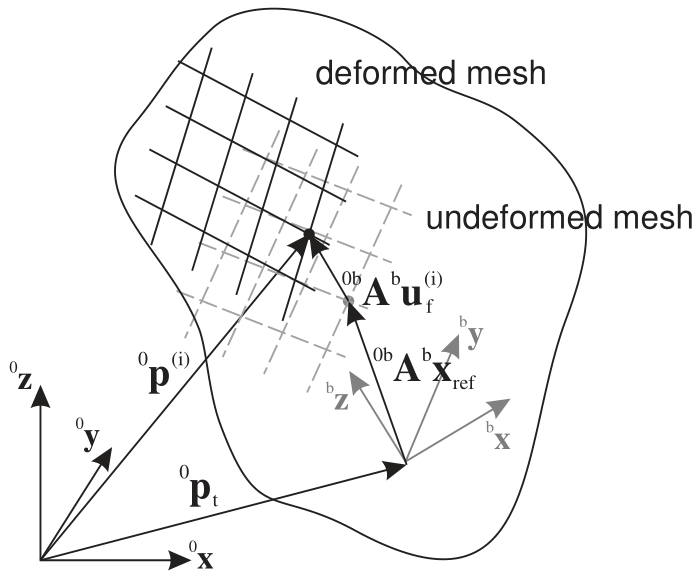
\includegraphics[width=8cm]{figures/ObjectFFRFsketch.pdf}
      \end{center}
      \caption{Floating frame of reference with exemplary position of a mesh node $i$.}
        \label{fig:ObjectFFRFreducedOrder:mesh}
    \end{figure}
    }
    \onlyRST{
    .. _fig-objectffrfreducedorder-mesh:
    .. figure:: docs/theDoc/figures/ObjectFFRFsketch.png
       :width: 400

       Floating frame of reference with exemplary position of a mesh node *i* 
    }
    %++++++++++++++++++++++++

                       
    The reduced order \hac{FFRF} formulation is based on an approximation of flexible coordinates $\LU{b}{\qv\indf}$ 
    by means of a reduction or mode basis $\LU{b}{\tPsi}$ (\texttt{modeBasis}) and the the modal coordinates $\tzeta$,
    \be
      \LU{b}{\qv\indf} \approx \LU{b}{\tPsi} \tzeta
    \ee
    The mode basis $\LU{b}{\tPsi}$ contains so-called mode shape vectors in its columns, which may be computed from eigen analysis, static computation or more advanced techniques, 
    see the helper functions in module \texttt{exudyn.FEM}, within the class \text{FEMinterface}.
    To compute eigen modes, use \texttt{FEMinterface.ComputeEigenmodes(...)} or
    \texttt{FEMinterface.ComputeHurtyCraigBamptonModes(...)}. For details on model order reduction and component mode synthesis, see \refSection{sec:theory:CMS}.
    In many applications, $n_m$ typically ranges between 10 and 50, but also beyond -- depending on the desired accuracy of the model.
    
    The \texttt{ObjectFFRF} coordinates and \eqs{eq:ObjectFFRF:eom}\footnote{this is not done for user functions and \texttt{forceVector}} can be reduced by the matrix $\Hm \in \Rcal^{(n\indf+n\indrigid) \times n_{ODE2}}$,
    \be
      \qv_{FFRF} = \vr{\qv\indt}{\ttheta}{\LU{b}{\qv\indf}} = \mr{\ImThree}{\Null}{\Null} {\Null}{\Im\indr}{\Null} {\Null}{\Null}{\LU{b}{\tPsi}} \vr{\qv\indt}{\ttheta}{\tzeta}
        = \Hm \, \qv
    \ee
    with the $4\times 4$ identity matrix $\Im\indr$ in case of Euler parameters and the reduced coordinates $\qv$.
    
    The reduced equations follow from the reduction of system matrices in \eqs{eq:ObjectFFRF:eom},
    \bea
      \Km\indred &=& \LU{b}{\tPsi}\tp \LU{b}{\Km} \LU{b}{\tPsi} \eqComma \\
      \Mm\indred &=& \LU{b}{\tPsi}\tp \LU{b}{\Mm} \LU{b}{\tPsi} \eqComma \\
    \eea
    the computation of rigid body inertia
    \bea
      \LU{b}{\tTheta}\indu &=& \LUX{b}{\tilde \xv}{\cRef\tp} \LU{b}{\Mm} \LU{b}{\tilde \xv\cRef}\\
    \eea
    the center of mass (and according tilde matrix), using $\tPhi\indt$ from \eq{eq:ObjectFFRF:Phit},
    \bea
      \LU{b}{\tchi}\indu &=& \frac{1}{m} \tPhi\tp\indt \LU{b}{\Mm} \LU{b}{\xv\cRef}\\
      \LU{b}{\tilde \tchi\indu} &=& \frac{1}{m} \tPhi\tp\indt \LU{b}{\Mm} \LU{b}{\tilde \xv\cRef}\\
    \eea 
    and seven inertia-like matrices \cite{ZwoelferGerstmayr2021},
    \be
      \Mm_{AB} = \Am\tp \LU{b}{\Mm} \Bm, \quad \mathrm{using} \quad \Am\Bm \in \left[\tPsi\tPsi ,\; \widetilde{\tPsi}\tPsi,\; \widetilde{\tPsi}\widetilde{\tPsi},\; 
        \tPhi\indt\tPsi,\; \tPhi\indt\widetilde{\tPsi},\; \tilde\xv\cRef\tPsi,\; \tilde\xv\cRef\widetilde{\tPsi}\right]
    \ee
    Note that the special tilde operator for vectors $\pv \in \Rcal^{n_f}$ of \eq{eq:ObjectFFRF:specialTilde} is frequently used.
    
    
    %+++++++++++++++++++++++++
    %+++++++++++++++++++++++++
    %+++++++++++++++++++++++++
    %+++++++++++++++++++++++++
    \mysubsubsubsection{Equations of motion}
    Equations of motion, in case that \texttt{computeFFRFterms = True}:
    \bea
        \left(\Mm_{user}(mbs, t,\qv,\dot \qv) + 
                    \mr{\Mm\indtt}{\Mm\indtr}{\Mm\indtf} {}{\Mm\indrr}{\Mm\indrf} {\mathrm{sym.}}{}{\Mm\indff} \right) \ddot \qv + 
                    \mr{0}{0}{0} {0}{0}{0} {0}{0}{\Dm\indff} \dot \qv + \mr{0}{0}{0} {0}{0}{0} {0}{0}{\Km\indff} \qv = &&\\ \nonumber
                    \fv_v(\qv,\dot \qv) + \fv_{user}(mbs, t,\qv,\dot \qv) &&
    \eea
    \footnote{NOTE that currently the internal (C++) computed terms are zero,
    \be
      \mr{\Mm\indtt}{\Mm\indtr}{\Mm\indtf} {}{\Mm\indrr}{\Mm\indrf} {\mathrm{sym.}}{}{\Mm\indff} = \Null \quad \mathrm{and} \quad
        \fv_v(\qv,\dot \qv) = \Null \eqComma
    \ee
    but they are implemented in predefined user functions, see \texttt{FEM.py}, \refSection{sec:FEM:ObjectFFRFreducedOrderInterface:AddObjectFFRFreducedOrderWithUserFunctions}. In near future, these terms will be implemented in C++ and replace the user functions.}
    %
    Note that in case of Euler parameters for the parameterization of rotations for the reference frame, the Euler parameter constraint equation is added automatically by this object.
    %
    The single terms of the mass matrix are defined as\cite{ZwoelferGerstmayr2021}
    \bea
      \Mm\indtt &=& m \ImThree \\
      \Mm\indtr &=& -\LU{0b}{\Rot} \left[ m \LU{b}{\tilde \tchi\indu} + \Mm_{\Phi\indt\!{\widetilde\Psi}} 
                      \left( \tzeta \otimes \Im \right)  \right] \LU{b}{\Gm}\\
      \Mm\indtf &=& \LU{0b}{\Rot} \Mm_{\Phi\indt\!\Psi} \\
      \Mm\indrr &=& \LU{b}{\Gm\tp} \left[\LU{b}{\tTheta}\indu + 
                                          \Mm_{\tilde \xv\cRef{\widetilde\Psi}} \left( \tzeta \otimes \Im \right) +
                                                                            \left( \tzeta \otimes \Im \right)\tp \Mm_{\tilde \xv\cRef{\widetilde\Psi}}\tp +
                                                                            \left( \tzeta \otimes \Im \right)\tp \Mm_{{\widetilde\Psi}{\widetilde\Psi}}\left( \tzeta \otimes \Im \right)
                                                                            \right] \LU{b}{\Gm}\\
      \Mm\indrf &=& -\LU{b}{\Gm\tp} \left[ \Mm_{\tilde \xv\cRef\Psi} + \left( \tzeta \otimes \Im \right)\tp \Mm_{{\widetilde\Psi}\Psi}  \right] \\ 
      \Mm\indff &=& \Mm_{\Psi\Psi}
    \eea
    with the Kronecker product\footnote{In Python numpy module this is computed by \texttt{numpy.kron(zeta, Im).T}},
    \be
      \tzeta \otimes \Im = \vr{\zeta_0 \Im}{\vdots}{\zeta_{m-1} \Im}
    \ee
    The quadratic velocity vector $\fv_v(\qv,\dot \qv) = \left[ \fv_{v\mathrm{t}}\tp,\; \fv_{v\mathrm{r}}\tp,\; \fv_{v\mathrm{f}}\tp \right]\tp$ reads
    \bea
      \fv_{v\mathrm{t}} &=& \LU{0b}{\Rot} \LU{b}{\tilde \tomega}\left[ m \LU{b}{\tilde \tchi\indu} + \Mm_{\Phi\indt\!{\widetilde\Psi}} 
                      \left( \tzeta \otimes \Im \right)  \right] \LU{b}{\tomega} + 
                                    2 \LU{0b}{\Rot} \Mm_{\Phi\indt\!{\widetilde\Psi}} \left( \dot \tzeta \otimes \Im \right)  \LU{b}{\tomega} \nonumber \\
                                && + \LU{0b}{\Rot} \left[ m \LU{b}{\tilde \tchi\indu} + \Mm_{\Phi\indt\!{\widetilde\Psi}} 
                      \left( \tzeta \otimes \Im \right)  \right] \LU{b}{\dot \Gm} \dot \ttheta \eqComma \\
        \fv_{v\mathrm{r}} &=& -\LU{b}{\Gm\tp} \LU{b}{\tilde \tomega} \left[\LU{b}{\tTheta}\indu + 
                                          \Mm_{\tilde \xv\cRef{\widetilde\Psi}} \left( \tzeta \otimes \Im \right) +
                                                                            \left( \tzeta \otimes \Im \right)\tp \Mm_{\tilde \xv\cRef{\widetilde\Psi}}\tp +
                                                                            \left( \tzeta \otimes \Im \right)\tp \Mm_{{\widetilde\Psi}{\widetilde\Psi}}\left( \tzeta \otimes \Im \right)
                                                                            \right]\LU{b}{\tomega} \nonumber \\
                                            && -2 \LU{b}{\Gm\tp} \left[ \Mm_{\tilde \xv\cRef{\widetilde\Psi}} \left( \dot \tzeta \otimes \Im \right) +
                                                                                        \left( \tzeta \otimes \Im \right)\tp \Mm_{{\widetilde\Psi}{\widetilde\Psi}}\left( \dot \tzeta \otimes \Im \right)
                                                                 \right] \LU{b}{\tomega} \nonumber \\
                                            && -\LU{b}{\Gm\tp}\left[\LU{b}{\tTheta}\indu + 
                                          \Mm_{\tilde \xv\cRef{\widetilde\Psi}} \left( \tzeta \otimes \Im \right) +
                                                                            \left( \tzeta \otimes \Im \right)\tp \Mm_{\tilde \xv\cRef{\widetilde\Psi}}\tp +
                                                                            \left( \tzeta \otimes \Im \right)\tp \Mm_{{\widetilde\Psi}{\widetilde\Psi}}\left( \tzeta \otimes \Im \right)
                                                                            \right] \LU{b}{\dot \Gm} \dot \ttheta \eqComma \\
        \fv_{v\mathrm{f}} &=& \left( \Im_\zeta \otimes \LU{b}{\tomega} \right)\tp 
                                    \left[ \Mm_{\tilde\xv\cRef{\widetilde\Psi}}\tp + \Mm_{{\widetilde\Psi}{\widetilde\Psi}}\left( \tzeta \otimes \Im \right) \right] \LU{b}{\tomega}
                                                                +2 \Mm_{{\widetilde\Psi}{\Psi}}\tp\left( \dot\tzeta \otimes \Im \right) \LU{b}{\tomega} \nonumber \\
                                            && + \left[ \Mm_{\tilde\xv\cRef{\Psi}}\tp + \Mm_{{\widetilde\Psi}{\Psi}}\tp\left( \tzeta \otimes \Im \right)
                                                 \right] \LU{b}{\dot \Gm} \dot \ttheta \eqDot
    \eea
    Note that terms including $\LU{b}{\dot \Gm} \dot \ttheta$ vanish in case of Euler parameters or in case that $\LU{b}{\dot \Gm} = \Null$,
    and we use another Kronecker product with the unit matrix $\Im_\zeta \in \Rcal^{n_m \times n_m}$,
    \be
      \Im_\zeta \otimes \LU{b}{\tomega} = \mr{\LU{b}{\tomega}}{}{} {}{\ddots}{} {}{}{\LU{b}{\tomega}} \in \Rcal^{3n_m \times n_m}
    \ee
    
    %$\ra$ will be completed later, see according literature of Zw{\"o}lfer and Gerstmayr \cite{ZwoelferGerstmayr2021}.
    
    In case that \texttt{computeFFRFterms = False}, the mass terms $\Mm\indtt \ldots \Mm\indff$ are zero (not computed) and
    the quadratic velocity vector $\fv_Q = \Null$.
    Note that the user functions $\fv_{user}(mbs, t,\qv,\dot \qv)$ and 
    $\Mm_{user}(mbs, t,\qv,\dot \qv)$ may be empty (=0). 
    The detailed equations of motion for this element can be found in \cite{ZwoelferGerstmayr2021}.

    %+++++++++++++++++++++++++
    %+++++++++++++++++++++++++
    \mysubsubsubsection{Position Jacobian}
    For joints and loads, the position jacobian of a node is needed in order to compute forces applied to averaged displacements and 
    rotations at nodes.
    Recall that the modal coordinates $\tzeta$ are transformed to node coordinates by means of the mode basis  $\LU{b}{\tPsi}$,
    \be
      \LU{b}{\qv\indf} = \LU{b}{\tPsi} \tzeta \eqDot
    \ee
    The local displacements $\LU{b}{\uv\indf^{(i)}}$ of a specific node $i$ can be reconstructed in this way by means of
    \be
      \LU{b}{\uv\indf^{(i)}} = \vr{\LU{b}{\qv_{\mathrm{f},i\cdot 3}}}{\LU{b}{\qv_{\mathrm{f},i\cdot 3+1}}}{\LU{b}{\qv_{\mathrm{f},i\cdot 3+2}}} \eqComma
    \ee
    and the global position of a node, see tables above, reads
    \be
      \LU{0}{\pv^{(i)}} = \LU{0}{\pv\indt} + \LU{0b}{\Am} \left( \LU{b}{\uv\indf^{(i)}} + \LU{b}{\xv^{(i)}\cRef} \right)
    \ee
    Thus, the jacobian of the global position reads
    \be
     \LU{0}{\Jm_\mathrm{pos}^{(i)}} = \frac{\partial \LU{0}{\pv^{(i)}}}{\partial [\qv\indt, \;\ttheta, \;\tzeta]}
     = \left[\ImThree, \; -\LU{0b}{\Rot} \left(\LU{b}{\tilde\uv\indf^{(i)}} + \LU{b}{\tilde\xv^{(i)}\cRef} \right) \LU{b}{\Gm},\;
             \LU{0b}{\Rot} \vr{\LU{b}{\tPsi_{r=3i}\tp}}{\LU{b}{\tPsi_{r=3i+1}\tp}}{\LU{b}{\tPsi_{r=3i+2}\tp}}\right] \eqComma
    \ee
    in which $\LU{b}{\tPsi_{r=...}}$ represents the row $r$ of the mode basis (matrix) $\LU{b}{\Psi}$, and
    the matrix 
    \be
      \vr{\LU{b}{\tPsi_{r=3i}\tp}}{\LU{b}{\tPsi_{r=3i+1}\tp}}{\LU{b}{\tPsi_{r=3i+2}\tp}} \in \Rcal^{3 \times n_m}
    \ee
    Furthermore, the jacobian of the local position reads
    \be
     \LU{b}{\Jm_\mathrm{pos}^{(i)}} = \frac{\partial \LU{b}{\pv\indf^{(i)}}}{\partial [\qv\indt, \;\ttheta, \;\tzeta]}
     = \left[\Null, \; \Null, \; \vr{\LU{b}{\tPsi_{r=3i}\tp}}{\LU{b}{\tPsi_{r=3i+1}\tp}}{\LU{b}{\tPsi_{r=3i+2}\tp}}\right] \eqComma
    \ee
    which is used in \texttt{MarkerSuperElementRigid}.
    
    
    %+++++++++++++++++++++++++
    %+++++++++++++++++++++++++
    \mysubsubsubsection{Joints and Loads}
    Use special \texttt{MarkerSuperElementPosition} to apply forces, SpringDampers or spherical joints. This marker can be attached to a single node of the underlying
    mesh or to a set of nodes, which is then averaged, see the according marker description.
    
    Use special \texttt{MarkerSuperElementRigid} to apply torques or special joints (e.g., \texttt{JointGeneric}). 
    This marker must be attached to a set of nodes which can represent rigid body motion. The rigid body motion is then averaged for all of these nodes,
    see the according marker description.
    
    For application of mass proportional loads (gravity), you can use conventional MarkerBodyMass.
    However, {\bf do not use} \texttt{MarkerBodyPosition} or \texttt{MarkerBodyRigid} for ObjectFFRFreducedOrder, unless wanted, because it only attaches to the floating
    frame. This means, that a force to a \texttt{MarkerBodyPosition} would only be applied to the (rigid) floating frame, but not onto the deformable body and
    results depend strongly on the choice of the reference frame (or the underlying mode shapes).
    
    CoordinateLoads are added for each \hac{ODE2} coordinate on the RHS of the equations of motion. 
    %++++++++++++++++++++++++++++++++++++++++
    
    
    %++++++++++++++++++++++++++++++++++++++++++++++++++++++++++
    \userFunction{forceUserFunction(mbs, t, itemNumber, q, q\_t)}
    A user function, which computes a force vector depending on current time and states of object. Can be used to create any kind of mechanical system by using the object states.
    Note that itemNumber represents the index of the ObjectFFRFreducedOrder object in mbs, which can be used to retrieve additional data from the object through
    \texttt{mbs.GetObjectParameter(itemNumber, ...)}, see the according description of \texttt{GetObjectParameter}.
    %
    \startTable{arguments /  return}{type or size}{description}
      \rowTable{\texttt{mbs}}{MainSystem}{provides MainSystem mbs to which object belongs}
      \rowTable{\texttt{t}}{Real}{current time in mbs}
      \rowTable{\texttt{itemNumber}}{Index}{integer number of the object in mbs, allowing easy access to all object data via mbs.GetObjectParameter(itemNumber, ...)}
      \rowTable{\texttt{q}}{Vector $\in \Rcal^n_{ODE2}$}{\hac{FFRF} object coordinates (rigid body coordinates and reduced coordinates in a list) in current configuration, without reference values}
      \rowTable{\texttt{q\_t}}{Vector $\in \Rcal^n_{ODE2}$}{object velocity coordinates (time derivatives of \texttt{q}) in current configuration}
      \rowTable{\returnValue}{Vector $\in \Rcal^{n_{ODE2}}$}{returns force vector for object}
    \finishTable
    %++++++++++++++++++++++++++++++++++++++++++++++++++++++++++
    \userFunction{massMatrixUserFunction(mbs, t, itemNumber, q, q\_t)}
    A user function, which computes a mass matrix depending on current time and states of object. Can be used to create any kind of mechanical system by using the object states.
    \startTable{arguments /  return}{type or size}{description}
      \rowTable{\texttt{mbs}}{MainSystem}{provides MainSystem mbs to which object belongs}
      \rowTable{\texttt{t}}{Real}{current time in mbs}
      \rowTable{\texttt{itemNumber}}{Index}{integer number of the object in mbs, allowing easy access to all object data via mbs.GetObjectParameter(itemNumber, ...)}
      \rowTable{\texttt{q}}{Vector $\in \Rcal^n_{ODE2}$}{\hac{FFRF} object coordinates (rigid body coordinates and reduced coordinates in a list) in current configuration, without reference values}
      \rowTable{\texttt{q\_t}}{Vector $\in \Rcal^n_{ODE2}$}{object velocity coordinates (time derivatives of \texttt{q}) in current configuration}
      \rowTable{\returnValue}{NumpyMatrix $\in \Rcal^{n_{ODE2} \times n_{ODE2}}$}{returns mass matrix for object}
    \finishTable
    \vspace{12pt}
    %++++++++++++++++++++++++++++++++++++++++++++++++++++++++++
    %%RSTCOMPATIBLE
\vspace{6pt}\par\noindent\rule{\textwidth}{0.4pt}
%
\noindent For examples on ObjectFFRFreducedOrder see Relevant Examples and TestModels with weblink:
\bi
\item \exuUrl{https://github.com/jgerstmayr/EXUDYN/blob/master/main/pythonDev/Examples/NGsolvePistonEngine.py}{\texttt{NGsolvePistonEngine.py}} (Examples/)
\item \exuUrl{https://github.com/jgerstmayr/EXUDYN/blob/master/main/pythonDev/Examples/objectFFRFreducedOrderNetgen.py}{\texttt{objectFFRFreducedOrderNetgen.py}} (Examples/)
\item \exuUrl{https://github.com/jgerstmayr/EXUDYN/blob/master/main/pythonDev/TestModels/NGsolveCrankShaftTest.py}{\texttt{NGsolveCrankShaftTest.py}} (TestModels/)
\item \exuUrl{https://github.com/jgerstmayr/EXUDYN/blob/master/main/pythonDev/TestModels/objectFFRFreducedOrderAccelerations.py}{\texttt{objectFFRFreducedOrderAccelerations.py}} (TestModels/)
\item \exuUrl{https://github.com/jgerstmayr/EXUDYN/blob/master/main/pythonDev/TestModels/objectFFRFreducedOrderShowModes.py}{\texttt{objectFFRFreducedOrderShowModes.py}} (TestModels/)
\item \exuUrl{https://github.com/jgerstmayr/EXUDYN/blob/master/main/pythonDev/TestModels/objectFFRFreducedOrderStressModesTest.py}{\texttt{objectFFRFreducedOrderStressModesTest.py}} (TestModels/)
\item \exuUrl{https://github.com/jgerstmayr/EXUDYN/blob/master/main/pythonDev/TestModels/superElementRigidJointTest.py}{\texttt{superElementRigidJointTest.py}} (TestModels/)

\ei

%

\newpage
%+++++++++++++++++++++++++++++++
%+++++++++++++++++++++++++++++++
\mysubsection{Objects (FiniteElement)}
A FiniteElement is a special Object and Body, which is used to define deformable bodies, such as beams or solid finite elements. FiniteElements are usually linked to two or more nodes.
%++++++

%+++++++++++++++++++++++++++++++++++

\mysubsubsection{ObjectANCFCable}
\label{sec:item:ObjectANCFCable}
A 3D cable finite element using 2 nodes of type NodePointSlope1. The localPosition of the beam with length $L$=physicsLength and height $h$ ranges in $X$-direction in range $[0, L]$ and in $Y$-direction in range $[-h/2,h/2]$ (which is in fact not needed in the \hac{EOM}). For description see ObjectANCFCable2D, which is almost identical to 3D case. Note that this element does not include torsion, therfore a torque cannot be applied along the local x-axis.
\vspace{12pt}\\

\noindent \mybold{Additional information for ObjectANCFCable}:
\bi
  \item This \texttt{Object} has/provides the following types = \texttt{Body}, \texttt{MultiNoded}
  \item Requested \texttt{Node} type = \texttt{Position}
  \item {\bf Short name} for Python = \texttt{Cable}
  \item {\bf Short name} for Python visualization object = \texttt{VCable}
\ei\vspace{12pt} \noindent 
The item \mybold{ObjectANCFCable} with type = 'ANCFCable' has the following parameters:
\vspace{-0.5cm}\\
\vspace{-0.5cm}\\
%reference manual TABLE
\begin{center}
  \footnotesize
  \begin{longtable}{| p{4.5cm} | p{2.5cm} | p{0.5cm} | p{2.5cm} | p{6cm} |}
    \hline
    \bf Name & \bf type & \bf size & \bf default value & \bf description \\ \hline
    name &     String &      &     '' &     objects's unique name\\ \hline
    physicsLength &     UReal &      &     0. &      [SI:m] reference length of beam; such that the total volume (e.g. for volume load) gives $\rho A L$; must be positive\\ \hline
    physicsMassPerLength &     UReal &      &     0. &      [SI:kg/m] mass per length of beam\\ \hline
    physicsBendingStiffness &     UReal &      &     0. &      [SI:Nm$^2$] bending stiffness of beam; the bending moment is $m = EI (\kappa - \kappa_0)$, in which $\kappa$ is the material measure of curvature\\ \hline
    physicsAxialStiffness &     UReal &      &     0. &      [SI:N] axial stiffness of beam; the axial force is $f_{ax} = EA (\varepsilon -\varepsilon_0)$, in which $\varepsilon = |\rv^\prime|-1$ is the axial strain\\ \hline
    physicsBendingDamping &     UReal &      &     0. &      [SI:Nm$^2$/s] bending damping of beam ; the additional virtual work due to damping is $\delta W_{\dot \kappa} = \int_0^L \dot \kappa \delta \kappa dx$\\ \hline
    physicsAxialDamping &     UReal &      &     0. &      [SI:N/s] axial damping of beam; the additional virtual work due to damping is $\delta W_{\dot\varepsilon} = \int_0^L \dot \varepsilon \delta \varepsilon dx$\\ \hline
    physicsReferenceAxialStrain &     Real &      &     0. &      [SI:1] reference axial strain of beam (pre-deformation) of beam; without external loading the beam will statically keep the reference axial strain value\\ \hline
    strainIsRelativeToReference &     Real &      &     0. &      if set to 1., a pre-deformed reference configuration is considered as the stressless state; if set to 0., the straight configuration plus the values of $\varepsilon_0$ and $\kappa_0$ serve as a reference geometry; allows also values between 0. and 1.\\ \hline
    nodeNumbers &     NodeIndex2 &      &     [invalid [-1], invalid [-1]] &     \tabnewline two node numbers ANCF cable element\\ \hline
    useReducedOrderIntegration &     Index &      &     0 &     0/false: use Gauss order 9 integration for virtual work of axial forces, order 5 for virtual work of bending moments; 1/true: use Gauss order 7 integration for virtual work of axial forces, order 3 for virtual work of bending moments\\ \hline
    visualization &     VObjectANCFCable &      &      &     parameters for visualization of item\\ \hline
\end{longtable}
\end{center}

\noindent The item VObjectANCFCable has the following parameters:
%reference manual TABLE
\begin{center}
  \footnotesize
  \begin{longtable}{| p{4.5cm} | p{2.5cm} | p{0.5cm} | p{2.5cm} | p{6cm} |}
    \hline
    \bf Name & \bf type & \bf size & \bf default value & \bf description \\ \hline
    show &     Bool &      &     True &     set true, if item is shown in visualization and false if it is not shown; note that all quantities are computed at the beam centerline, even if drawn on surface of cylinder of beam; this effects, e.g., Displacement or Velocity, which is drawn constant over cross section\\ \hline
    radius &     float &      &     0. &     if radius==0, only the centerline is drawn; else, a cylinder with radius is drawn; circumferential tiling follows general.cylinderTiling and beam axis tiling follows bodies.beams.axialTiling\\ \hline
    color &     Float4 &      &     [-1.,-1.,-1.,-1.] &     \tabnewline RGBA color of the object; if R==-1, use default color\\ \hline
\end{longtable}
\end{center}
\par\noindent\rule{\textwidth}{0.4pt}
\mysubsubsubsection{DESCRIPTION of ObjectANCFCable:}
\label{description_ObjectANCFCable}
\paragraph{Information on input parameters:} 
\startTable{input parameter}{symbol}{description see tables above}
\rowTable{physicsLength}{$L$}{}
\rowTable{physicsMassPerLength}{$\rho A$}{}
\rowTable{physicsBendingStiffness}{$EI$}{}
\rowTable{physicsAxialStiffness}{$EA$}{}
\rowTable{physicsBendingDamping}{$d_{K}$}{}
\rowTable{physicsAxialDamping}{$d_{\varepsilon}$}{}
\rowTable{physicsReferenceAxialStrain}{$\varepsilon_0$}{}
\rowTable{strainIsRelativeToReference}{$f\cRef$}{}
\finishTable

\mybold{The following output variables are available as OutputVariableType in sensors, Get...Output() and other functions}:
\begin{center}
\footnotesize
\begin{longtable}{| p{5cm} | p{5cm} | p{6cm} |} 
\hline
\bf output variable & \bf symbol & \bf description \\ \hline
Position & $\LU{0}{\pv\cConfig(x,0,0)} = \rv\cConfig(x) + y\cdot \nv\cConfig(x)$ & global position vector of local position $[x,0,0]$\\ \hline
Displacement & $\LU{0}{\uv\cConfig(x,0,0)} = \LU{0}{\pv\cConfig(x,0,0)} - \LU{0}{\pv\cRef(x,0,0)}$ & global displacement vector of local position\\ \hline
Velocity & $\LU{0}{\vv(x,0,0)} = \LU{0}{\dot \rv(x)}$ & global velocity vector of local position\\ \hline
Director1 & $\rv'(x)$ & (axial) slope vector of local axis position (at $y$=0)\\ \hline
StrainLocal & $\varepsilon$ & axial strain (scalar) of local axis position (at Y=Z=0)\\ \hline
CurvatureLocal & $[K_x, K_y, K_z]\tp$ & local curvature vector\\ \hline
ForceLocal & $N$ &  (local) section normal force (scalar, including reference strains) (at $y$=$z$=0); note that strains are highly inaccurate when coupled to bending, thus consider useReducedOrderIntegration=2 and evaluate axial strain at nodes or at midpoint\\ \hline
TorqueLocal & $M$ &  (local) bending moment (scalar) (at $y$=$z$=0), which are bending moments as there is no torque\\ \hline
Acceleration & $\LU{0}{\av(x,0,0)} = \LU{0}{\ddot \rv(x)}$ & global acceleration vector of local position\\ \hline
\end{longtable}
\end{center}
 \noindent
    %%RSTCOMPATIBLE
\vspace{6pt}\par\noindent\rule{\textwidth}{0.4pt}
\mysubsubsubsection{MINI EXAMPLE for ObjectANCFCable}
\label{miniExample_ObjectANCFCable}
\pythonstyle
\begin{lstlisting}[language=Python, firstnumber=1]
    from exudyn.beams import GenerateStraightLineANCFCable
    rhoA = 78.
    EA = 1000000.
    EI = 833.3333333333333
    cable = Cable(physicsMassPerLength=rhoA, 
                  physicsBendingStiffness=EI, 
                  physicsAxialStiffness=EA, 
                  )

    ancf=GenerateStraightLineANCFCable(mbs=mbs,
                  positionOfNode0=[0,0,0], positionOfNode1=[2,0,0],
                  numberOfElements=32, #converged to 4 digits
                  cableTemplate=cable, #this defines the beam element properties
                  massProportionalLoad = [0,-9.81,0],
                  fixedConstraintsNode0 = [1,1,1, 0,1,1], #add constraints for pos and rot (r'_y,r'_z)
                  )
    lastNode = ancf[0][-1]

    #assemble and solve system for default parameters
    mbs.Assemble()
    mbs.SolveStatic()

    #check result
    exudynTestGlobals.testResult = mbs.GetNodeOutput(lastNode, exu.OutputVariableType.Displacement)[0]
    #ux=-0.5013058140308901
\end{lstlisting}

\newpage

%+++++++++++++++++++++++++++++++++++

\mysubsubsection{ObjectANCFCable2D}
\label{sec:item:ObjectANCFCable2D}
A 2D cable finite element using 2 nodes of type NodePoint2DSlope1. The localPosition of the beam with length $L$=physicsLength and height $h$ ranges in $X$-direction in range $[0, L]$ and in $Y$-direction in range $[-h/2,h/2]$ (which is in fact not needed in the \hac{EOM}).
\vspace{12pt}\\

\noindent \mybold{Additional information for ObjectANCFCable2D}:
\bi
  \item Requested \texttt{Node} type = \texttt{Position2D} + \texttt{Orientation2D} + \texttt{Point2DSlope1} + \texttt{Position} + \texttt{Orientation}
  \item {\bf Short name} for Python = \texttt{Cable2D}
  \item {\bf Short name} for Python visualization object = \texttt{VCable2D}
\ei\vspace{12pt} \noindent 
The item \mybold{ObjectANCFCable2D} with type = 'ANCFCable2D' has the following parameters:
\vspace{-0.5cm}\\
\vspace{-0.5cm}\\
%reference manual TABLE
\begin{center}
  \footnotesize
  \begin{longtable}{| p{4.5cm} | p{2.5cm} | p{0.5cm} | p{2.5cm} | p{6cm} |}
    \hline
    \bf Name & \bf type & \bf size & \bf default value & \bf description \\ \hline
    name &     String &      &     '' &     objects's unique name\\ \hline
    physicsLength &     UReal &      &     0. &      [SI:m] reference length of beam; such that the total volume (e.g. for volume load) gives $\rho A L$; must be positive\\ \hline
    physicsMassPerLength &     UReal &      &     0. &      [SI:kg/m] mass per length of beam\\ \hline
    physicsBendingStiffness &     UReal &      &     0. &      [SI:Nm$^2$] bending stiffness of beam; the bending moment is $m = EI (\kappa - \kappa_0)$, in which $\kappa$ is the material measure of curvature\\ \hline
    physicsAxialStiffness &     UReal &      &     0. &      [SI:N] axial stiffness of beam; the axial force is $f_{ax} = EA (\varepsilon -\varepsilon_0)$, in which $\varepsilon = |\rv^\prime|-1$ is the axial strain\\ \hline
    physicsBendingDamping &     UReal &      &     0. &      [SI:Nm$^2$/s] bending damping of beam ; the additional virtual work due to damping is $\delta W_{\dot \kappa} = \int_0^L \dot \kappa \delta \kappa dx$\\ \hline
    physicsAxialDamping &     UReal &      &     0. &      [SI:N/s] axial damping of beam; the additional virtual work due to damping is $\delta W_{\dot\varepsilon} = \int_0^L \dot \varepsilon \delta \varepsilon dx$\\ \hline
    physicsReferenceAxialStrain &     Real &      &     0. &      [SI:1] reference axial strain of beam (pre-deformation) of beam; without external loading the beam will statically keep the reference axial strain value\\ \hline
    physicsReferenceCurvature &     Real &      &     0. &      [SI:1/m] reference curvature of beam (pre-deformation) of beam; without external loading the beam will statically keep the reference curvature value\\ \hline
    strainIsRelativeToReference &     Real &      &     0. &      if set to 1., a pre-deformed reference configuration is considered as the stressless state; if set to 0., the straight configuration plus the values of $\varepsilon_0$ and $\kappa_0$ serve as a reference geometry; allows also values between 0. and 1.\\ \hline
    nodeNumbers &     NodeIndex2 &      &     [invalid [-1], invalid [-1]] &     \tabnewline two node numbers ANCF cable element\\ \hline
    useReducedOrderIntegration &     Index &      &     0 &     0/false: use Gauss order 9 integration for virtual work of axial forces, order 5 for virtual work of bending moments; 1/true: use Gauss order 7 integration for virtual work of axial forces, order 3 for virtual work of bending moments\\ \hline
    axialForceUserFunction &     PyFunctionMbsScalarIndexScalar9 &     \tabnewline  &     \tabnewline 0 &     A Python function which defines the (nonlinear relations) of local strains (including axial strain and bending strain) as well as time derivatives to the local axial force; see description below\\ \hline
    bendingMomentUserFunction &     PyFunctionMbsScalarIndexScalar9 &     \tabnewline  &     \tabnewline 0 &     A Python function which defines the (nonlinear relations) of local strains (including axial strain and bending strain) as well as time derivatives to the local bending moment; see description below\\ \hline
    visualization &     VObjectANCFCable2D &      &      &     parameters for visualization of item\\ \hline
\end{longtable}
\end{center}

\noindent The item VObjectANCFCable2D has the following parameters:
%reference manual TABLE
\begin{center}
  \footnotesize
  \begin{longtable}{| p{4.5cm} | p{2.5cm} | p{0.5cm} | p{2.5cm} | p{6cm} |}
    \hline
    \bf Name & \bf type & \bf size & \bf default value & \bf description \\ \hline
    show &     Bool &      &     True &     set true, if item is shown in visualization and false if it is not shown\\ \hline
    drawHeight &     float &      &     0. &     if beam is drawn with rectangular shape, this is the drawing height\\ \hline
    color &     Float4 &      &     [-1.,-1.,-1.,-1.] &     \tabnewline RGBA color of the object; if R==-1, use default color\\ \hline
\end{longtable}
\end{center}
\par\noindent\rule{\textwidth}{0.4pt}
\mysubsubsubsection{DESCRIPTION of ObjectANCFCable2D:}
\label{description_ObjectANCFCable2D}
\paragraph{Information on input parameters:} 
\startTable{input parameter}{symbol}{description see tables above}
\rowTable{physicsLength}{$L$}{}
\rowTable{physicsMassPerLength}{$\rho A$}{}
\rowTable{physicsBendingStiffness}{$EI$}{}
\rowTable{physicsAxialStiffness}{$EA$}{}
\rowTable{physicsBendingDamping}{$d_{K}$}{}
\rowTable{physicsAxialDamping}{$d_{\varepsilon}$}{}
\rowTable{physicsReferenceAxialStrain}{$\varepsilon_0$}{}
\rowTable{physicsReferenceCurvature}{$\kappa_0$}{}
\rowTable{strainIsRelativeToReference}{$f\cRef$}{}
\rowTable{axialForceUserFunction}{$\mathrm{UF} \in \Rcal$}{}
\rowTable{bendingMomentUserFunction}{$\mathrm{UF} \in \Rcal$}{}
\finishTable

\mybold{The following output variables are available as OutputVariableType in sensors, Get...Output() and other functions}:
\begin{center}
\footnotesize
\begin{longtable}{| p{5cm} | p{5cm} | p{6cm} |} 
\hline
\bf output variable & \bf symbol & \bf description \\ \hline
Position & $\LU{0}{\pv\cConfig(x,y,0)} = \rv\cConfig(x) + y\cdot \nv\cConfig(x)$ & global position vector of local position $[x,y,0]$\\ \hline
Displacement & $\LU{0}{\uv\cConfig(x,y,0)} = \LU{0}{\pv\cConfig(x,y,0)} - \LU{0}{\pv\cRef(x,y,0)}$ & global displacement vector of local position\\ \hline
Velocity & $\LU{0}{\vv(x,y,0)} = \LU{0}{\dot \rv(x)} - y \cdot \omega_2 \cdot\LU{0}{\tv(x)} $ & global velocity vector of local position\\ \hline
VelocityLocal & $\LU{b}{\vv(x,y,0)} = \LU{b0}{\Rot}\LU{0}{\vv(x,y,0)}$ & local velocity vector of local position\\ \hline
Rotation & $\varphi = \mathrm{atan2}(r'_y, r'_x)$ & (scalar) rotation angle of axial slope vector (relative to global $x$-axis)\\ \hline
Director1 & $\rv'(x)$ & (axial) slope vector of local axis position (at $y$=0)\\ \hline
StrainLocal & $\varepsilon$ & axial strain (scalar) of local axis position (at Y=0)\\ \hline
CurvatureLocal & $K$ & axial strain (scalar)\\ \hline
ForceLocal & $N$ &  (local) section normal force (scalar, including reference strains) (at $y$=0); note that strains are highly inaccurate when coupled to bending, thus consider useReducedOrderIntegration=2 and evaluate axial strain at nodes or at midpoint\\ \hline
TorqueLocal & $M$ &  (local) bending moment (scalar) (at $y$=0)\\ \hline
AngularVelocity & $\tomega = [0,\, ,0,\, \omega_2]$ & angular velocity of local axis position (at $y$=0)\\ \hline
Acceleration & $\LU{0}{\av(x,y,0)} = \LU{0}{\ddot \rv(x)} - y \cdot \dot\omega_2 \cdot\LU{0}{\tv(x)}- y \cdot \omega_2 \cdot\LU{0}{\dot\tv(x)} $ & global acceleration vector of local position\\ \hline
AngularAcceleration & $\talpha = [0,\, ,0,\, \dot\omega_2]$ & angular acceleration of local axis position\\ \hline
\end{longtable}
\end{center}
 \noindent
    \mysubsubsubsection{Definition of quantities}
    \startTable{intermediate variables}{symbol}{description}
      \rowTable{beam height}{$h$}{beam height used in several definitions, but effectively undefined. The geometry of the cross section has no influence except for drawing or contact.}
      \rowTable{local beam position}{$\pLocB=[x,\, y,\, 0]\tp$}{local position at axial coordinate $x \in [0,L]$ and cross section coordinate $y \in [-h/2, h/2]$. }
      \rowTable{beam axis position}{$\LU{0}{\rv(x)} = \rv(x) $}{}
      \rowTable{beam axis slope}{$\LU{0}{\rv'(x)} = \rv'(x) $}{}
      \rowTable{beam axis tangent}{$\LU{0}{\tv(x)} = \frac{\rv'(x)}{\Vert \rv(x)'\Vert} $}{this (normalized) vector is normal to cross section}
      \rowTable{beam axis normal}{$\LU{0}{\nv(x)} = [n_x,\, n_y]\tp = [-t_y,\, t_x]\tp  $}{this (normalized) vector lies within the cross section and defines positive $y$-direction.}
      \rowTable{angular velocity}{$\omega_2 = (-r'_y \cdot \dot r'_x + r'_x \cdot \dot r'_y) / \Vert \rv(x)'\Vert^2 $}{}
      \rowTable{rotation matrix}{$\LU{0b}{\Rot}$}{}
      %\rowTable{}{$\LU{0}{\fv} $}{}
      %\rowTable{}{$\LU{0}{\fv} $}{}
    \finishTable

    The Bernoulli-Euler beam is capable of large axial and bendig deformation as it employs the material measure of curvature for the bending.
    %
    \mysubsubsubsection{Kinematics and interpolation}
    %
    Note that in this section, expressions are written in 2D, while output variables are in general 3D quantities, adding a zero for the $z$-coordinate.
    %
    ANCF elements follow the original concept proposed by Shabana \cite{shabana1997ancf}.
    The present 2D element is based on the interpolation used by Berzeri and Shabana \cite{berzeri2000}, but the formulation (especially of the elastic forces) is according to
    Gerstmayr and Irschik \cite{GerstmayrIrschik2008}.
    Slight improvements for the integration of elastic forces and additional terms for off-axis forces and constraints are mentioned here.
    
    The current position of an arbitrary element at local axial position $x \in [0,L]$, where $L$ is the beam length, reads
    \be
      \rv=\rv(x, t),
    \ee
    The derivative of the position w.r.t.\ the axial reference coordinate is denoted as slope vector,
    \be
      \rv'= \frac{\partial \rv(x, t)}{\partial x}
    \ee
    The interpolation is based on cubic (spline) interpolation of position, displacements and velocities.
    The generalized coordinates $\qv \in \Rcal^8$ of the beam element is defined by
    \be
      \qv= \left[\, \rv_0^{T}\;\;\rv_0^{' T}\;\; \rv_1^{T}\;\; \rv_1^{' T}\, \right]^{T}.
    \ee
    in which $\rv_0$ is the position of node 0 and $\rv_1$ is the position of node 1,
    $\rv'_0$ the slope at node 0 and $\rv'_1$ the slope at node 1.
    Note that ANCF coordinates in the present notation are computed as sum of reference and current coordinates
    \be
      \qv = \qv\cCur + \qv\cRef
    \ee
    which is used throughout here. For time derivatives, it follows that $\dot \qv = \dot \qv\cCur$.
    
    Position and slope are interpolated with shape functions.
    The position and slope along the beam are interpolated by means of 
    \be
      \rv = \Sm \qv \qquad \mathrm{and} \qquad \rv'=\Sm' \qv.
    \ee
    in which $\Sm$ is the shape function matrix,
    \be
      \Sm(x)= \left[\, S_1(x)\,\ImTwo\;\; S_2(x)\,\ImTwo\;\; S_3(x)\,\ImTwo\;\; S_4(x)\,\ImTwo\, \right].
    \ee
    with identity matrix $\ImTwo \in \Rcal^{2 \times 2}$ and the shape functions
    \bea \label{eq:cable2D:shapeFunctions}
      S_1(x) &=& 1-3\frac{x^2}{L^2}+2\frac{x^3}{L^3}, \quad
      S_2(x) = x-2\frac{x^2}{L}+\frac{x^3}{L^2}\nonumber\\
      S_3(x) &=& 3\frac{x^2}{L^2}-2\frac{x^3}{L^3}, \; \; \; \; \; \;  \quad
      S_4(x) = -\frac{x^2}{L}+\frac{x^3}{L^2}
    \eea
    %
    Velocity simply follows as 
    \be
      \frac{\partial \rv}{\partial t} = \dot \rv = \Sm \dot \qv.
    \ee
    %
    \mysubsubsubsection{Mass matrix}
    The mass matrix is constant and therefore precomputed at the first time it is needed (e.g., during computation of initial accelerations).
    The analytical form of the mass matrix reads
    \be
       \Mm_{analytic} = \int_0^L \rho A \Sm(x)^T \Sm(x) dx
    \ee
    which is approximated using
    \be
       \Mm = \sum_{ip = 0}^{n_{ip}-1} w(x_{ip}) \frac{L}{2} \rho A \Sm(x_{ip})^T \Sm(x_{ip})
    \ee
    with integration weights $w(x_{ip})$, $\sum w(x_{ip})=2$, and integration points $x_{ip}$, given as,
    \be \label{eq_ANCFCable_ipTransform}
      x_{ip} = \frac{L}{2}\xi_{ip} + \frac{L}{2} \eqDot
    \ee
    Here, we use the Gauss integration rule with order 7, having $n_{ip}=4$ Gauss points, see \refSection{sec:integrationPoints}. 
    Due to the third order polynomials, the integration is exact up to round-off errors.
            
    \mysubsubsubsection{Elastic forces}
    The elastic forces $\Qm_e$ are implicitly defined by the relation to the 
    virtual work of elastic forces, $\delta W_e$, of applied forces, $\delta W_a$ and of viscous forces, $\delta W_v$, 
    \be \label{eq:cable2D:elasticForces}
      \Qm_e^T \delta \qv = \delta W_e + \delta W_a + \delta W_v.
    \ee
    The virtual work of elastic forces reads \cite{GerstmayrIrschik2008},
    \be
      \delta W_e = \int_0^L (N \delta \varepsilon + M \delta K) \,dx,
    \ee
    %\todo{compute $\delta W_e = \Qm_e^T \delta \qv$ }
    in which the axial strain is defined as \cite{GerstmayrIrschik2008}
    \be
      \varepsilon=\Vert \rv'\Vert-1.
    \ee 
    and the material measure of curvature (bending strain) is given as
    \be
        K=\ev_3^T \frac{ \rv'\times \rv'' }{\Vert \rv'\Vert^2} .
    \ee
    %\todo{define vector e3}
    in which $\ev_3$ is the unit vector which is perpendicular to the plane of the planar beam element.
    
    By derivation, we obtain the variation of axial strain
    \be \label{eq:cable2D:deltaEpsilon}
    \delta \varepsilon =\frac{\partial \varepsilon}{\partial q_i}\delta q_i
      %= \frac{\rv'^{T}\frac{\partial}{\partial q_i}\rv'}{\Vert \rv' \Vert} \delta q_i
    %=\frac{1}{\Vert \rv' \Vert}\rv'^{T}\frac{\partial \rv'}{\partial q_i}\delta q_i\nonumber\\
        =\frac{1}{\Vert \rv'\Vert}\rv'^{T}\Sm'_i \delta q_i.
    \ee
    and the variation of $K$
    \bea \label{eq:cable2D:deltaKappa}
    \delta K &=& \frac{\partial}{\partial q_i} \left( \frac{(\rv'^{T}\times \rv'' )^{T}\ev_{3}}{\Vert \rv' \Vert^2 }\right) \delta q_i\nonumber\\
       &=& \frac{1}{\Vert \rv' \Vert^4} \left[ \Vert \rv' \Vert^2 (\Sm'_i  \times \rv'' +\rv' \times \Sm''_i) -2 (\rv' \times \rv'') (\rv'^{T} \Sm'_i) \right]^{T} \ev_3 \delta q_i
    \eea
    The normal force (axial force) $N$ in the beam is defined as function of the current strain $\varepsilon$,
    \be \label{eq_N}
      N = EA \, (\varepsilon - \varepsilon_0 - f\cRef \cdot \varepsilon\cRef).
    \ee
    in which $\varepsilon_0$ includes the (pre-)stretch of the beam, e.g., due to temperature or plastic deformation and 
    $\varepsilon\cRef$ includes the strain of the reference configuration.
    As can be seen, the reference strain is only considered, if $f\cRef=1$, which allows to consider the reference configuration to be
    completely stress-free (but the default value is $f\cRef=0$ !).
    Note that -- due to the inherent nonlinearity of $\varepsilon$ -- a combination of $\varepsilon_0$ and $f\cRef=1$ is physically only meaningful for small strains.
    A factor $f\cRef<1$ allows to realize a smooth transition between deformed and straight reference configuration, e.g. for initial configurations.

    The bending moment $M$ in the beam is defined as function of the current material measure of curvature $K$,
    \be \label{eq_M}
      M = EI \, (K - K_0 - f\cRef \cdot K\cRef).
    \ee
    in which $K_0$ includes the (pre-)curvature of the undeformed beam and
    $K\cRef$ includes the curvature of the reference configuration, multiplied with the factor $f\cRef=1$, see the axial strain above.

    Using the latter definitions, the elastic forces follow from \eq{eq:cable2D:elasticForces}.
    
    The virtual work of viscous damping forces, assuming viscous effects proportial to axial streching and bending, is defined as
    \be
      \delta W_v = \int_0^L \left( d_\varepsilon \dot \varepsilon \delta \varepsilon + d_K \dot K \delta K \right) \,d x.
    \ee
    with material coefficients $d_\varepsilon$ and $d_K$.
    The time derivatives of axial strain $\dot \varepsilon_p$ follows by elementary differentiation
    \be
      \dot \varepsilon =  \frac{\partial }{\partial t}\left(\Vert \rv'\Vert-1 \right)
        %= \frac{\rv^{\prime T} \frac{\partial}{\partial t}\rv'}{\Vert \rv'\Vert} 
        = \frac{1}{\Vert \rv'\Vert} \rv^{\prime T} \Sm' \dot \qv
    \ee
    as well as the derivative of the curvature,
    \bea
        \dot K & = &  \frac{\partial }{\partial t}\left(\ev_3^T\frac{ \rv'\times \rv'' }{\Vert \rv'\Vert^2}\right) \nonumber\\
                 & = &\frac{\ev_3^T}{(\rv'^T \rv')^2} \left( (\rv'^T \rv')   \frac{\partial \left( \rv' \times \rv'' \right)^T }{\partial t} -\left( \rv' \times \rv'' \right)^T  \frac{\partial  (\rv'^T \rv')}{\partial t} \right)\nonumber\\
                 %& = & \frac{\ev_3^T}{(\rv'^T \rv')^2} \left((\rv'^T \rv') \left( \frac {\partial \rv''}{\partial t} \times \rv''+ \frac{\partial \rv''}{\partial t} \times \rv' \right)-\left( \rv' \times \rv'' \right) \left(2\rv'^T \frac{\partial \rv'}{\partial t}\right) \right) \nonumber\\
                 & = &  \frac{\ev_3^T}{(\rv'^T \rv')^2}\left((\rv'^T \rv')\left((\Sm' \dot \qv) \times \rv'' + (\Sm'' \dot \qv) \times \rv'\right)-\left( \rv' \times \rv'' \right) (2\rv'^T (\Sm' \dot \qv)) \right) .
    \eea
    
    The virtual work of applied forces reads
    \be
    \label{eq_applied}
    \delta W_a = \sum_i \fv_i^T \delta \rv_i(x_f) + \int_0^L \bv^T \delta \rv(x) \,d x \eqComma
    \ee
    in which $\fv_i$ are forces applied to a certain position $x_f$ at the beam centerline.
    The second term contains a load per length $\bv$, which is case of gravity vector $\gv$ reads
    \be
      \bv = \rho \gv.
    \ee
    Note that the variation of $\rv$ simply follows as
    \be
      \delta \rv= \Sm\, \delta \qv
    \ee

    \mysubsubsubsection{Numerical integration of Elastic Forces}
    The numerical integration of elastic forces $\Qm_e$ is split into terms due to $\delta \varepsilon$ and $\delta K$,
    \be
      \Qm_e = \int_0^L \left(\bullet(x) \frac{\partial \delta \varepsilon}{\partial \delta \qv} + \bullet(x) \frac{\partial \delta K}{\partial \delta \qv} \right) \,dx
    \ee
    using different integration rules
    \be
      \Qm_e \approx  \sum_{ip = 0}^{n_{ip}^\varepsilon-1}  \left(\frac{L}{2}  \bullet(x_{ip}) \frac{\partial \delta \varepsilon}{\partial \delta \qv} \right)
                   + \sum_{ip = 0}^{n_{ip}^K-1} \left( \frac{L}{2}\bullet(x_{ip}) \frac{\partial \delta K}{\partial \delta \qv} \right) \,dx
    \ee
    with the integration points $x_{ip}$ as defined in \eq{eq_ANCFCable_ipTransform} and integration rules from \refSection{sec:integrationPoints}.
    There are 3 different options for integration rules depending on the flag \texttt{useReducedOrderIntegration}:
    \bn
      \item \texttt{useReducedOrderIntegration} = 0: $n_{ip}^\varepsilon = 5$ (Gauss order 9), $n_{ip}^K = 3$ (Gauss order 5) -- this is considered as full integration, leading to very small approximations; certainly, due to the high nonlinearity of expressions, this is only an approximation.
      \item \texttt{useReducedOrderIntegration} = 1: $n_{ip}^\varepsilon = 4$ (Gauss order 7), $n_{ip}^K = 2$ (Gauss order 3) -- this is considered as reduced integration, which is usually sufficiently accurate but leads to slightly less computational efforts, especially for bending terms.
      \item \texttt{useReducedOrderIntegration} = 2: $n_{ip}^\varepsilon = 3$ (Lobatto order 3), $n_{ip}^K = 2$ (Gauss order 3) -- this is a further reduced integration, with the exceptional property that axial strain and bending strain terms are computed at completely disjointed locations: axial strain terms are evaluated at $0$, $L/2$ and $L$, while bending terms are evaluated at $\frac{L}{2} \pm \frac{L}{2}\sqrt{1/3}$. This allows axial strains to freely follow the bending terms at $\frac{L}{2} \pm \frac{L}{2}\sqrt{1/3}$, while axial strains are almost independent from bending terms at $0$, $L/2$ and $L$. However, due to the highly reduced integration, spurious (hourglass) modes may occur in certain applications!
    \en
    Note that the Jacobian of elastic forces is computed using automatic differentiation.
    
    \mysubsubsubsection{Access functions}
    For application of forces and constraints at any local beam position $\pLocB=[x,\, y,\, 0]\tp$, the position / velocity Jacobian reads
    \be
      \frac{\partial \LU{0}{\vv(x)}}{\dot \qv} = \Sm(x) + \left[ -y \cdot n_x S'_1(x) \frac{1}{\Vert \rv'\Vert} \LU{0}{\tv}, \,\, 
        -y \cdot n_y S'_1(x) \frac{1}{\Vert \rv'\Vert} \LU{0}{\tv}, \,\, -y \cdot n_x S'_2(x) \frac{1}{\Vert \rv'\Vert} \LU{0}{\tv}, \,\,\ldots \right]
    \ee
    with the normalized beam axis normal $\LU{0}{\nv} = [n_x,\, n_y]\tp$, see table above.

    For application of torques at any axis point $x$, the rotation / angular velocity Jacobian $\frac{\partial \LU{0}{\omega(x)}}{\dot \qv} \in \Rcal^{3 \times 8}$ reads
    \be
      \frac{\partial \LU{0}{\omega(x)}}{\dot \qv} = 
       \left[\!\! \begin{array}{ccccc} 
      0 & 0 & 0 & \cdots & 0 \vspace{0.1cm}\\ 
      0 & 0 & 0 & \cdots & 0 \vspace{0.1cm}\\ 
      -r'_y \cdot S'_1(x) \frac{1}{\rv^{\prime 2}} & r'_x \cdot S'_1(x) \frac{1}{\rv^{\prime 2}} & 
      -r'_y \cdot S'_2(x) \frac{1}{\rv^{\prime 2}} & \cdots & r'_x \cdot S'_4(x) \frac{1}{\rv^{\prime 2}}  \end{array} \!\!\right]
    \ee
    %++++++++++++++++++++++++++++++++++++++++++++++++++++++++++
    \userFunction{axialForceUserFunction(mbs, t, itemNumber, axialPositionNormalized, axialStrain, axialStrain\_t, axialStrainRef, physicsAxialStiffness, physicsAxialDamping, curvature, curvature\_t, curvatureRef)}
    A user function, which computes the axial force depending on time, strains and curvatures and 
    object parameters (stiffness, damping).
    The object variables are provided to the function using the current values of the ANCFCable2D object.
    Note that itemNumber represents the index of the object in mbs, which can be used to retrieve additional data from the object through
    \texttt{mbs.GetObjectParameter(itemNumber, ...)}, see the according description of \texttt{GetObjectParameter}.
    \mybold{NOTE:} this function has a different interface as compared to the bending moment function.
    %
    \startTable{arguments /  return}{type or size}{description}
      \rowTable{\texttt{mbs}}{MainSystem}{provides MainSystem mbs to which object belongs}
      \rowTable{\texttt{t}}{Real}{current time in mbs}
      \rowTable{\texttt{itemNumber}}{Index}{integer number $i_N$ of the object in mbs, allowing easy access to all object data via mbs.GetObjectParameter(itemNumber, ...)}
      \rowTable{\texttt{axialPositionNormalized}}{Real}{axial position at the cable where the user function is evaluated; range is [0,1]}
      \rowTable{\texttt{axialStrain}}{Real}{$\varepsilon$}
      \rowTable{\texttt{axialStrain\_t}}{Real}{$\varepsilon_t$}
      \rowTable{\texttt{axialStrainRef}}{Real}{$\varepsilon_0 + f\cRef \cdot \varepsilon\cRef$}
      \rowTable{\texttt{physicsAxialStiffness}}{Real}{as given in object parameters}
      \rowTable{\texttt{physicsAxialDamping}}{Real}{as given in object parameters}
      \rowTable{\texttt{curvature}}{Real}{$K$}
      \rowTable{\texttt{curvature\_t}}{Real}{$\dot K$}
      \rowTable{\texttt{curvatureRef}}{Real}{$K_0 + f\cRef \cdot K\cRef$}
      \rowTable{\returnValue}{Real}{scalar value of computed axial force}
    \finishTable
    %++++++++++++++++++++++++++++++++++++++++++++++++++++++++++
    \userFunction{bendingMomentUserFunction(mbs, t, itemNumber, axialPositionNormalized, curvature, curvature\_t, curvatureRef, physicsBendingStiffness, physicsBendingDamping, axialStrain, axialStrain\_t, axialStrainRef)}
    A user function, which computes the bending moment depending on time, strains and curvatures and 
    object parameters (stiffness, damping).
    The object variables are provided to the function using the current values of the ANCFCable2D object.
    Note that itemNumber represents the index of the object in mbs, which can be used to retrieve additional data from the object through
    \texttt{mbs.GetObjectParameter(itemNumber, ...)}, see the according description of \texttt{GetObjectParameter}.
    \mybold{NOTE:} this function has a different interface as compared to the axial force function.
    %
    \startTable{arguments /  return}{type or size}{description}
      \rowTable{\texttt{mbs}}{MainSystem}{provides MainSystem mbs to which object belongs}
      \rowTable{\texttt{t}}{Real}{current time in mbs}
      \rowTable{\texttt{itemNumber}}{Index}{integer number $i_N$ of the object in mbs, allowing easy access to all object data via mbs.GetObjectParameter(itemNumber, ...)}
      \rowTable{\texttt{axialPositionNormalized}}{Real}{axial position at the cable where the user function is evaluated; range is [0,1]}
      \rowTable{\texttt{curvature}}{Real}{$K$}
      \rowTable{\texttt{curvature\_t}}{Real}{$\dot K$}
      \rowTable{\texttt{curvatureRef}}{Real}{$K_0 + f\cRef \cdot K\cRef$}
      \rowTable{\texttt{physicsBendingStiffness}}{Real}{as given in object parameters}
      \rowTable{\texttt{physicsBendingDamping}}{Real}{as given in object parameters}
      \rowTable{\texttt{axialStrain}}{Real}{$\varepsilon$}
      \rowTable{\texttt{axialStrain\_t}}{Real}{$\varepsilon_t$}
      \rowTable{\texttt{axialStrainRef}}{Real}{$\varepsilon_0 + f\cRef \cdot \varepsilon\cRef$}
      \rowTable{\returnValue}{Real}{scalar value of computed bending moment}
    \finishTable
    %
    %++++++++++++++++++++++++++++++++++++++++++++++++++++++++++
    \userFunctionExample{}
    \pythonstyle\begin{lstlisting}
        #define some material parameters
        rhoA = 100.
        EA =   1e7.
        EI =   1e5

        #example of bending moment user function
        def bendingMomentUserFunction(mbs, t, itemNumber, axialPositionNormalized, 
                   curvature, curvature_t, curvatureRef, physicsBendingStiffness, 
                   physicsBendingDamping, axialStrain, axialStrain_t, axialStrainRef):
            fact = min(1,t) #runs from 0 to 1
            #change reference curvature of beam over time:
            kappa=(curvature-curvatureRef*fact) 
            return physicsBendingStiffness*(kappa) + physicsBendingDamping*curvature_t

        def axialForceUserFunction(mbs, t, itemNumber, axialPositionNormalized, 
                   axialStrain, axialStrain_t, axialStrainRef, physicsAxialStiffness, 
                   physicsAxialDamping, curvature, curvature_t, curvatureRef):
            fact = min(1,t) #runs from 0 to 1
            return (physicsAxialStiffness*(axialStrain-fact*axialStrainRef) + 
                    physicsAxialDamping*axialStrain_t)

        cable = ObjectANCFCable2D(physicsMassPerLength=rhoA, 
                        physicsBendingStiffness=EI, 
                        physicsBendingDamping = EI*0.1,
                        physicsAxialStiffness=EA,
                        physicsAxialDamping=EA*0.05,
                        physicsReferenceAxialStrain=0.1, #10% stretch
                        physicsReferenceCurvature=1,     #radius=1
                        bendingMomentUserFunction=bendingMomentUserFunction,
                        axialForceUserFunction=axialForceUserFunction,
                        )
        #use  cable with GenerateStraightLineANCFCable(...)
    \end{lstlisting} \vspace{12pt}
    %%RSTCOMPATIBLE
\vspace{6pt}\par\noindent\rule{\textwidth}{0.4pt}
\mysubsubsubsection{MINI EXAMPLE for ObjectANCFCable2D}
\label{miniExample_ObjectANCFCable2D}
\pythonstyle
\begin{lstlisting}[language=Python, firstnumber=1]
    rhoA = 78.
    EA = 1000000.
    EI = 833.3333333333333
    cable = Cable2D(physicsMassPerLength=rhoA, 
                    physicsBendingStiffness=EI, 
                    physicsAxialStiffness=EA, 
                    )

    ancf=GenerateStraightLineANCFCable2D(mbs=mbs,
                    positionOfNode0=[0,0,0], positionOfNode1=[2,0,0],
                    numberOfElements=32, #converged to 4 digits
                    cableTemplate=cable, #this defines the beam element properties
                    massProportionalLoad = [0,-9.81,0],
                    fixedConstraintsNode0 = [1,1,0,1], #add constraints for pos and rot (r'_y)
                    )
    lastNode = ancf[0][-1]

    #assemble and solve system for default parameters
    mbs.Assemble()
    mbs.SolveStatic()

    #check result
    exudynTestGlobals.testResult = mbs.GetNodeOutput(lastNode, exu.OutputVariableType.Displacement)[0]
    #ux=-0.5013058140308901
\end{lstlisting}

\vspace{6pt}\par\noindent\rule{\textwidth}{0.4pt}
%
\noindent For examples on ObjectANCFCable2D see Relevant Examples and TestModels with weblink:
\bi
\item \exuUrl{https://github.com/jgerstmayr/EXUDYN/blob/master/main/pythonDev/Examples/sliderCrank3DwithANCFbeltDrive2.py}{\texttt{sliderCrank3DwithANCFbeltDrive2.py}} (Examples/)
\item \exuUrl{https://github.com/jgerstmayr/EXUDYN/blob/master/main/pythonDev/Examples/ALEANCFpipe.py}{\texttt{ALEANCFpipe.py}} (Examples/)
\item \exuUrl{https://github.com/jgerstmayr/EXUDYN/blob/master/main/pythonDev/Examples/ANCFcantileverTest.py}{\texttt{ANCFcantileverTest.py}} (Examples/)
\item \exuUrl{https://github.com/jgerstmayr/EXUDYN/blob/master/main/pythonDev/Examples/ANCFcantileverTestDyn.py}{\texttt{ANCFcantileverTestDyn.py}} (Examples/)
\item \exuUrl{https://github.com/jgerstmayr/EXUDYN/blob/master/main/pythonDev/Examples/ANCFcontactCircle.py}{\texttt{ANCFcontactCircle.py}} (Examples/)
\item \exuUrl{https://github.com/jgerstmayr/EXUDYN/blob/master/main/pythonDev/Examples/ANCFcontactCircle2.py}{\texttt{ANCFcontactCircle2.py}} (Examples/)
\item \exuUrl{https://github.com/jgerstmayr/EXUDYN/blob/master/main/pythonDev/Examples/ANCFmovingRigidbody.py}{\texttt{ANCFmovingRigidbody.py}} (Examples/)
\item \exuUrl{https://github.com/jgerstmayr/EXUDYN/blob/master/main/pythonDev/Examples/ANCFrotatingCable2D.py}{\texttt{ANCFrotatingCable2D.py}} (Examples/)
\item \exuUrl{https://github.com/jgerstmayr/EXUDYN/blob/master/main/pythonDev/Examples/ANCFslidingJoint2D.py}{\texttt{ANCFslidingJoint2D.py}} (Examples/)
\item \exuUrl{https://github.com/jgerstmayr/EXUDYN/blob/master/main/pythonDev/Examples/ANCFslidingJoint2Drigid.py}{\texttt{ANCFslidingJoint2Drigid.py}} (Examples/)
\item \exuUrl{https://github.com/jgerstmayr/EXUDYN/blob/master/main/pythonDev/Examples/ANCFswitchingSlidingJoint2D.py}{\texttt{ANCFswitchingSlidingJoint2D.py}} (Examples/)
\item \exuUrl{https://github.com/jgerstmayr/EXUDYN/blob/master/main/pythonDev/Examples/ANCFtestHalfcircle.py}{\texttt{ANCFtestHalfcircle.py}} (Examples/)
\item  ...

\item \exuUrl{https://github.com/jgerstmayr/EXUDYN/blob/master/main/pythonDev/TestModels/ANCFcontactCircleTest.py}{\texttt{ANCFcontactCircleTest.py}} (TestModels/)
\item \exuUrl{https://github.com/jgerstmayr/EXUDYN/blob/master/main/pythonDev/TestModels/ANCFcontactFrictionTest.py}{\texttt{ANCFcontactFrictionTest.py}} (TestModels/)
\item \exuUrl{https://github.com/jgerstmayr/EXUDYN/blob/master/main/pythonDev/TestModels/computeODE2EigenvaluesTest.py}{\texttt{computeODE2EigenvaluesTest.py}} (TestModels/)
\item  ...


\ei

%
\newpage

%+++++++++++++++++++++++++++++++++++

\mysubsubsection{ObjectALEANCFCable2D}
\label{sec:item:ObjectALEANCFCable2D}
A 2D cable finite element using 2 nodes of type NodePoint2DSlope1 and a axially moving coordinate of type NodeGenericODE2, which adds additional (redundant) motion in axial direction of the beam. This allows modeling pipes but also axially moving beams. The localPosition of the beam with length $L$=physicsLength and height $h$ ranges in $X$-direction in range $[0, L]$ and in $Y$-direction in range $[-h/2,h/2]$ (which is in fact not needed in the \hac{EOM}).
\vspace{12pt}\\

\noindent \mybold{Additional information for ObjectALEANCFCable2D}:
\bi
  \item Requested \texttt{Node} type: read detailed information of item
  \item {\bf Short name} for Python = \texttt{ALECable2D}
  \item {\bf Short name} for Python visualization object = \texttt{VALECable2D}
\ei\vspace{12pt} \noindent 
The item \mybold{ObjectALEANCFCable2D} with type = 'ALEANCFCable2D' has the following parameters:
\vspace{-0.5cm}\\
\vspace{-0.5cm}\\
%reference manual TABLE
\begin{center}
  \footnotesize
  \begin{longtable}{| p{4.5cm} | p{2.5cm} | p{0.5cm} | p{2.5cm} | p{6cm} |}
    \hline
    \bf Name & \bf type & \bf size & \bf default value & \bf description \\ \hline
    name &     String &      &     '' &     objects's unique name\\ \hline
    physicsLength &     UReal &      &     0. &      [SI:m] reference length of beam; such that the total volume (e.g. for volume load) gives $\rho A L$; must be positive\\ \hline
    physicsMassPerLength &     UReal &      &     0. &      [SI:kg/m] total mass per length of beam (including axially moving parts / fluid)\\ \hline
    physicsMovingMassFactor &     UReal &      &     1. &     this factor denotes the amount of $\rho A$ which is moving; physicsMovingMassFactor=1 means, that all mass is moving; physicsMovingMassFactor=0 means, that no mass is moving; factor can be used to simulate e.g. pipe conveying fluid, in which $\rho A$ is the mass of the pipe+fluid, while $physicsMovingMassFactor \cdot \rho A$ is the mass per unit length of the fluid\\ \hline
    physicsBendingStiffness &     UReal &      &     0. &      [SI:Nm$^2$] bending stiffness of beam; the bending moment is $m = EI (\kappa - \kappa_0)$, in which $\kappa$ is the material measure of curvature\\ \hline
    physicsAxialStiffness &     UReal &      &     0. &      [SI:N] axial stiffness of beam; the axial force is $f_{ax} = EA (\varepsilon -\varepsilon_0)$, in which $\varepsilon = |\rv^\prime|-1$ is the axial strain\\ \hline
    physicsBendingDamping &     UReal &      &     0. &      [SI:Nm$^2$/s] bending damping of beam ; the additional virtual work due to damping is $\delta W_{\dot \kappa} = \int_0^L \dot \kappa \delta \kappa dx$\\ \hline
    physicsAxialDamping &     UReal &      &     0. &      [SI:N/s] axial damping of beam; the additional virtual work due to damping is $\delta W_{\dot\varepsilon} = \int_0^L \dot \varepsilon \delta \varepsilon dx$\\ \hline
    physicsReferenceAxialStrain &     Real &      &     0. &      [SI:1] reference axial strain of beam (pre-deformation) of beam; without external loading the beam will statically keep the reference axial strain value\\ \hline
    physicsReferenceCurvature &     Real &      &     0. &      [SI:1/m] reference curvature of beam (pre-deformation) of beam; without external loading the beam will statically keep the reference curvature value\\ \hline
    physicsUseCouplingTerms &     Bool &      &     True &     true: correct case, where all coupling terms due to moving mass are respected; false: only include constant mass for ALE node coordinate, but deactivate other coupling terms (behaves like ANCFCable2D then)\\ \hline
    physicsAddALEvariation &     Bool &      &     True &     true: correct case, where additional terms related to variation of strain and curvature are added\\ \hline
    nodeNumbers &     NodeIndex3 &      &     [invalid [-1], invalid [-1], invalid [-1]] &     \tabnewline two node numbers ANCF cable element, third node=ALE GenericODE2 node\\ \hline
    useReducedOrderIntegration &     Index &      &     0 &     0/false: use Gauss order 9 integration for virtual work of axial forces, order 5 for virtual work of bending moments; 1/true: use Gauss order 7 integration for virtual work of axial forces, order 3 for virtual work of bending moments\\ \hline
    strainIsRelativeToReference &     Real &      &     0. &      if set to 1., a pre-deformed reference configuration is considered as the stressless state; if set to 0., the straight configuration plus the values of $\varepsilon_0$ and $\kappa_0$ serve as a reference geometry; allows also values between 0. and 1.\\ \hline
    visualization &     VObjectALEANCFCable2D &      &      &     parameters for visualization of item\\ \hline
\end{longtable}
\end{center}

\noindent The item VObjectALEANCFCable2D has the following parameters:
%reference manual TABLE
\begin{center}
  \footnotesize
  \begin{longtable}{| p{4.5cm} | p{2.5cm} | p{0.5cm} | p{2.5cm} | p{6cm} |}
    \hline
    \bf Name & \bf type & \bf size & \bf default value & \bf description \\ \hline
    show &     Bool &      &     True &     set true, if item is shown in visualization and false if it is not shown\\ \hline
    drawHeight &     float &      &     0. &     if beam is drawn with rectangular shape, this is the drawing height\\ \hline
    color &     Float4 &      &     [-1.,-1.,-1.,-1.] &     \tabnewline RGBA color of the object; if R==-1, use default color\\ \hline
\end{longtable}
\end{center}
\par\noindent\rule{\textwidth}{0.4pt}
\mysubsubsubsection{DESCRIPTION of ObjectALEANCFCable2D:}
\label{description_ObjectALEANCFCable2D}
\paragraph{Information on input parameters:} 
\startTable{input parameter}{symbol}{description see tables above}
\rowTable{physicsLength}{$L$}{}
\rowTable{physicsMassPerLength}{$\rho A$}{}
\rowTable{physicsBendingStiffness}{$EI$}{}
\rowTable{physicsAxialStiffness}{$EA$}{}
\rowTable{physicsBendingDamping}{$d_{K}$}{}
\rowTable{physicsAxialDamping}{$d_{\varepsilon}$}{}
\rowTable{physicsReferenceAxialStrain}{$\varepsilon_0$}{}
\rowTable{physicsReferenceCurvature}{$\kappa_0$}{}
\rowTable{strainIsRelativeToReference}{$f\cRef$}{}
\finishTable

\mybold{The following output variables are available as OutputVariableType in sensors, Get...Output() and other functions}:
\begin{center}
\footnotesize
\begin{longtable}{| p{5cm} | p{5cm} | p{6cm} |} 
\hline
\bf output variable & \bf symbol & \bf description \\ \hline
Position &  & global position vector of local position (in X/Y beam coordinates)\\ \hline
Displacement &  & global displacement vector of local position\\ \hline
Velocity &  & global velocity vector of local position\\ \hline
VelocityLocal &  & local velocity vector of local position\\ \hline
Rotation &  & (scalar) rotation angle of axial slope vector (relative to global x-axis)\\ \hline
Director1 &  & (axial) slope vector of local axis position (at Y=0)\\ \hline
StrainLocal & $\varepsilon$ & axial strain (scalar) of local axis position (at Y=0)\\ \hline
CurvatureLocal & $K$ & axial strain (scalar)\\ \hline
ForceLocal & $N$ &  (local) section normal force (scalar, including reference strains) (at Y=0); note that strains are highly inaccurate when coupled to bending, thus consider useReducedOrderIntegration=2 and evaluate axial strain at nodes or at midpoint\\ \hline
TorqueLocal & $M$ &  (local) bending moment (scalar) (at Y=0)\\ \hline
\end{longtable}
\end{center}
 \noindent
    A 2D cable finite element using 2 nodes of type NodePoint2DSlope1 and an axially moving coordinate of type NodeGenericODE2.
    The element has 8+1 coordinates and uses cubic polynomials for position interpolation.
    In addition to ANCFCable2D the element adds an Eulerian axial velocity by the GenericODE2 coordiante.
    The parameter \texttt{physicsMovingMassFactor} allows to control the amount of mass, which moves with
    the Eulerian velocity (e.g., the fluid), and which is not moving (the pipe). 
    A factor of \texttt{physicsMovingMassFactor=1} gives an axially moving beam.

    The Bernoulli-Euler beam is capable of large deformation as it employs the material measure of curvature for the bending.
    Note that damping (physicsBendingDamping, physicsAxialDamping) only acts on the non-moving part of the beam, as it is the case for the pipe.
    
    Note that most functions act on the underlying cable finite element, which is not co-moving axially. E.g., if you apply constraints
    to the nodal coordinates, the cable can be fixed, while still the axial component is freely moving.
    If you apply a LoadForce using a MarkerPosition, the force is acting on the beam finite element, but not on the axially moving coordinate.
    In contrast to the latter, the ObjectJointALEMoving2D and the MarkerBodyMass are acting on the moving coordinate as well.

    A detailed paper on this element is yet under submission, but a similar formulation can be found in \cite{PechsteinGerstmayr2013ale} and 
    the underlying beam element is identical to ObjectANCFCable2D.
    %%RSTCOMPATIBLE
\vspace{6pt}\par\noindent\rule{\textwidth}{0.4pt}
%
\noindent For examples on ObjectALEANCFCable2D see Relevant Examples and TestModels with weblink:
\bi
\item \exuUrl{https://github.com/jgerstmayr/EXUDYN/blob/master/main/pythonDev/Examples/ALEANCFpipe.py}{\texttt{ALEANCFpipe.py}} (Examples/)
\item \exuUrl{https://github.com/jgerstmayr/EXUDYN/blob/master/main/pythonDev/Examples/ANCFALEtest.py}{\texttt{ANCFALEtest.py}} (Examples/)
\item \exuUrl{https://github.com/jgerstmayr/EXUDYN/blob/master/main/pythonDev/Examples/ANCFmovingRigidbody.py}{\texttt{ANCFmovingRigidbody.py}} (Examples/)
\item \exuUrl{https://github.com/jgerstmayr/EXUDYN/blob/master/main/pythonDev/Examples/flexiblePendulumANCF.py}{\texttt{flexiblePendulumANCF.py}} (Examples/)
\item \exuUrl{https://github.com/jgerstmayr/EXUDYN/blob/master/main/pythonDev/TestModels/ANCFoutputTest.py}{\texttt{ANCFoutputTest.py}} (TestModels/)

\ei

%
\newpage

%+++++++++++++++++++++++++++++++++++

\mysubsubsection{ObjectANCFBeam}
\label{sec:item:ObjectANCFBeam}
OBJECT UNDER CONSTRUCTION: A 3D beam finite element based on the absolute nodal coordinate formulation, using two nodes. The localPosition $x$ of the beam ranges from $-L/2$ (at node 0) to $L/2$ (at node 1). The axial coordinate is $x$ (first coordinate) and the cross section is spanned by local $y$/$z$ axes; assuming dimensions $w_y$ and $w_z$ in cross section, the local position range is $\in [[-L/2,L/2],\, [-wy/2,wy/2],\, [-wz/2,wz/2] ]$.
\vspace{12pt}\\

\noindent \mybold{Additional information for ObjectANCFBeam}:
\bi
  \item This \texttt{Object} has/provides the following types = \texttt{Body}, \texttt{MultiNoded}
  \item Requested \texttt{Node} type = \texttt{Position} + \texttt{Orientation}
  \item {\bf Short name} for Python = \texttt{ANCFBeam}
  \item {\bf Short name} for Python visualization object = \texttt{VANCFBeam}
\ei\vspace{12pt} \noindent 
The item \mybold{ObjectANCFBeam} with type = 'ANCFBeam' has the following parameters:
\vspace{-0.5cm}\\
\vspace{-0.5cm}\\
%reference manual TABLE
\begin{center}
  \footnotesize
  \begin{longtable}{| p{4.5cm} | p{2.5cm} | p{0.5cm} | p{2.5cm} | p{6cm} |}
    \hline
    \bf Name & \bf type & \bf size & \bf default value & \bf description \\ \hline
    name &     String &      &     '' &     objects's unique name\\ \hline
    nodeNumbers &     NodeIndex2 &      &     [invalid [-1], invalid [-1]] &     \tabnewline two node numbers for beam element\\ \hline
    physicsLength &     PReal &      &     0. &      [SI:m] reference length of beam; such that the total volume (e.g. for volume load) gives $\rho A L$; must be positive\\ \hline
    sectionData &     BeamSection &      &     BeamSection() &     data as given by exudyn.BeamSection(), defining inertial, stiffness and damping parameters of beam section.\\ \hline
    crossSectionPenaltyFactor &     Vector3D &      &     [1.,1.,1.] &     \tabnewline  [SI:1] additional penalty factors for cross section deformation, which are in total $k_{cs} = [f_{yy}\cdot k_{yy},\, f_{zz}\cdot k_{zz},\, f_{yz}\cdot k_{yz}]\tp$\\ \hline
    visualization &     VObjectANCFBeam &      &      &     parameters for visualization of item\\ \hline
\end{longtable}
\end{center}

\noindent The item VObjectANCFBeam has the following parameters:
%reference manual TABLE
\begin{center}
  \footnotesize
  \begin{longtable}{| p{4.5cm} | p{2.5cm} | p{0.5cm} | p{2.5cm} | p{6cm} |}
    \hline
    \bf Name & \bf type & \bf size & \bf default value & \bf description \\ \hline
    show &     Bool &      &     True &     set true, if item is shown in visualization and false if it is not shown; geometry is defined by sectionGeometry\\ \hline
    sectionGeometry &     BeamSectionGeometry &     \tabnewline  &     \tabnewline BeamSectionGeometry() &     \tabnewline defines cross section shape used for visualization and contact\\ \hline
    color &     Float4 &      &     [-1.,-1.,-1.,-1.] &     \tabnewline RGBA color of the object; if R==-1, use default color\\ \hline
\end{longtable}
\end{center}
\par\noindent\rule{\textwidth}{0.4pt}
\mysubsubsubsection{DESCRIPTION of ObjectANCFBeam:}
\label{description_ObjectANCFBeam}
\paragraph{Information on input parameters:} 
\startTable{input parameter}{symbol}{description see tables above}
\rowTable{physicsLength}{$L$}{}
\rowTable{crossSectionPenaltyFactor}{$f_{cs} = [f_{yy},\,f_{zz},\,f_{yz}]\tp$}{}
\finishTable

\mybold{The following output variables are available as OutputVariableType in sensors, Get...Output() and other functions}:
\begin{center}
\footnotesize
\begin{longtable}{| p{5cm} | p{5cm} | p{6cm} |} 
\hline
\bf output variable & \bf symbol & \bf description \\ \hline
Position &  & global position vector of local position vector\\ \hline
Displacement &  & global displacement vector of local position vector\\ \hline
Velocity &  & global velocity vector of local position vector\\ \hline
VelocityLocal &  & global velocity vector of local position vector\\ \hline
AngularVelocity &  & global angular velocity vector of local (axis) position vector\\ \hline
AngularVelocityLocal &  & local angular velocity vector of local (axis) position vector\\ \hline
Acceleration &  & global acceleration vector of local position vector\\ \hline
Rotation &  & 3D Tait-Bryan rotation components of cross section rotation\\ \hline
RotationMatrix &  & rotation matrix of cross section rotation as 9D vector\\ \hline
\end{longtable}
\end{center}
 \noindent
    Detailed description coming later.
    %%RSTCOMPATIBLE
\vspace{6pt}\par\noindent\rule{\textwidth}{0.4pt}
%
\noindent For examples on ObjectANCFBeam see Relevant Examples and TestModels with weblink:
\bi
\item \exuUrl{https://github.com/jgerstmayr/EXUDYN/blob/master/main/pythonDev/TestModels/ANCFBeamEigTest.py}{\texttt{ANCFBeamEigTest.py}} (TestModels/)
\item \exuUrl{https://github.com/jgerstmayr/EXUDYN/blob/master/main/pythonDev/TestModels/ANCFBeamTest.py}{\texttt{ANCFBeamTest.py}} (TestModels/)
\item \exuUrl{https://github.com/jgerstmayr/EXUDYN/blob/master/main/pythonDev/TestModels/geometricallyExactBeamTest.py}{\texttt{geometricallyExactBeamTest.py}} (TestModels/)
\item \exuUrl{https://github.com/jgerstmayr/EXUDYN/blob/master/main/pythonDev/TestModels/rightAngleFrame.py}{\texttt{rightAngleFrame.py}} (TestModels/)

\ei

%
\newpage

%+++++++++++++++++++++++++++++++++++

\mysubsubsection{ObjectBeamGeometricallyExact2D}
\label{sec:item:ObjectBeamGeometricallyExact2D}
A 2D geometrically exact beam finite element, currently using 2 nodes of type NodeRigidBody2D; FURTHER TESTS REQUIRED. Note that the orientation of the nodes need to follow the cross section orientation in case that includeReferenceRotations=True; e.g., an angle 0 represents the cross section aligned with the $y$-axis, while and angle $\pi/2$ means that the cross section points in negative $x$-direction. Pre-curvature can be included with physicsReferenceCurvature and axial pre-stress can be considered by using a physicsLength different from the reference configuration of the nodes. The localPosition of the beam with length $L$=physicsLength and height $h$ ranges in $X$-direction in range $[-L/2, L/2]$ and in $Y$-direction in range $[-h/2,h/2]$ (which is in fact not needed in the \hac{EOM}).
\vspace{12pt}\\

\noindent \mybold{Additional information for ObjectBeamGeometricallyExact2D}:
\bi
  \item This \texttt{Object} has/provides the following types = \texttt{Body}, \texttt{MultiNoded}
  \item Requested \texttt{Node} type = \texttt{Position2D} + \texttt{Orientation2D} + \texttt{Position} + \texttt{Orientation}
  \item {\bf Short name} for Python = \texttt{Beam2D}
  \item {\bf Short name} for Python visualization object = \texttt{VBeam2D}
\ei\vspace{12pt} \noindent 
The item \mybold{ObjectBeamGeometricallyExact2D} with type = 'BeamGeometricallyExact2D' has the following parameters:
\vspace{-0.5cm}\\
\vspace{-0.5cm}\\
%reference manual TABLE
\begin{center}
  \footnotesize
  \begin{longtable}{| p{4.5cm} | p{2.5cm} | p{0.5cm} | p{2.5cm} | p{6cm} |}
    \hline
    \bf Name & \bf type & \bf size & \bf default value & \bf description \\ \hline
    name &     String &      &     '' &     objects's unique name\\ \hline
    nodeNumbers &     NodeIndex2 &      &     [invalid [-1], invalid [-1]] &     \tabnewline two node numbers for beam element\\ \hline
    physicsLength &     UReal &      &     0. &      [SI:m] reference length of beam; such that the total volume (e.g. for volume load) gives $\rho A L$; must be positive\\ \hline
    physicsMassPerLength &     UReal &      &     0. &      [SI:kg/m] mass per length of beam\\ \hline
    physicsCrossSectionInertia &     UReal &      &     0. &      [SI:kg m] cross section mass moment of inertia; inertia acting against rotation of cross section\\ \hline
    physicsBendingStiffness &     UReal &      &     0. &      [SI:Nm$^2$] bending stiffness of beam; the bending moment is $m = EI (\kappa - \kappa_0)$, in which $\kappa$ is the material measure of curvature\\ \hline
    physicsAxialStiffness &     UReal &      &     0. &      [SI:N] axial stiffness of beam; the axial force is $f_{ax} = EA (\varepsilon -\varepsilon_0)$, in which $\varepsilon$ is the axial strain\\ \hline
    physicsShearStiffness &     UReal &      &     0. &      [SI:N] effective shear stiffness of beam, including stiffness correction\\ \hline
    physicsBendingDamping &     UReal &      &     0. &      [SI:Nm$^2$/s] viscous damping of bending deformation; the additional virtual work due to damping is $\delta W_{\dot \kappa} = \int_0^L \dot \kappa \delta \kappa dx$\\ \hline
    physicsAxialDamping &     UReal &      &     0. &      [SI:N/s] viscous damping of axial deformation\\ \hline
    physicsShearDamping &     UReal &      &     0. &      [SI:N/s] viscous damping of shear deformation\\ \hline
    physicsReferenceCurvature &     Real &      &     0. &      [SI:1/m] reference curvature of beam (pre-deformation) of beam\\ \hline
    includeReferenceRotations &     bool &      &     False &     if True, rotations at nodes consider reference rotations, which are used for the computation of bending strains (this means that a pre-curved beam is stress-free); if False, the reference rotation of the cross section is orthogonal to the direction between the reference position of the end nodes. This allows to easily share nodes among several beams with different cross section orientation.\\ \hline
    visualization &     VObjectBeamGeometricallyExact2D &      &      &     parameters for visualization of item\\ \hline
\end{longtable}
\end{center}

\noindent The item VObjectBeamGeometricallyExact2D has the following parameters:
%reference manual TABLE
\begin{center}
  \footnotesize
  \begin{longtable}{| p{4.5cm} | p{2.5cm} | p{0.5cm} | p{2.5cm} | p{6cm} |}
    \hline
    \bf Name & \bf type & \bf size & \bf default value & \bf description \\ \hline
    show &     Bool &      &     True &     set true, if item is shown in visualization and false if it is not shown\\ \hline
    drawHeight &     float &      &     0. &     if beam is drawn with rectangular shape, this is the drawing height\\ \hline
    color &     Float4 &      &     [-1.,-1.,-1.,-1.] &     \tabnewline RGBA color of the object; if R==-1, use default color\\ \hline
\end{longtable}
\end{center}
\par\noindent\rule{\textwidth}{0.4pt}
\mysubsubsubsection{DESCRIPTION of ObjectBeamGeometricallyExact2D:}
\label{description_ObjectBeamGeometricallyExact2D}
\paragraph{Information on input parameters:} 
\startTable{input parameter}{symbol}{description see tables above}
\rowTable{physicsLength}{$L$}{}
\rowTable{physicsMassPerLength}{$\rho A$}{}
\rowTable{physicsCrossSectionInertia}{$\rho J$}{}
\rowTable{physicsBendingStiffness}{$EI$}{}
\rowTable{physicsAxialStiffness}{$EA$}{}
\rowTable{physicsShearStiffness}{$GA$}{}
\rowTable{physicsBendingDamping}{$d_{K}$}{}
\rowTable{physicsAxialDamping}{$d_{\varepsilon}$}{}
\rowTable{physicsShearDamping}{$d_{\gamma}$}{}
\rowTable{physicsReferenceCurvature}{$\kappa_0$}{}
\finishTable

\mybold{The following output variables are available as OutputVariableType in sensors, Get...Output() and other functions}:
\begin{center}
\footnotesize
\begin{longtable}{| p{5cm} | p{5cm} | p{6cm} |} 
\hline
\bf output variable & \bf symbol & \bf description \\ \hline
Position &  & global position vector of local axis (X) and cross section (Y) position\\ \hline
Displacement &  & global displacement vector of local axis (X) and cross section (Y) position\\ \hline
Velocity &  & global velocity vector of local axis (X) and cross section (Y) position\\ \hline
Rotation &  & 3D Tait-Bryan rotation components, containing rotation around $Z$-axis only\\ \hline
StrainLocal &  & 6 (local) strain components, containing only axial ($XX$, index 0) and shear strain ($XY$, index 5); evaluated at beam axis ONLY\\ \hline
CurvatureLocal &  & 3D vector of (local) curvature, only $Z$ component is non-zero\\ \hline
ForceLocal &  & 3D vector of (local) section normal force, containing axial (X) and shear force (Y)\\ \hline
TorqueLocal &  & 3D vector of (local) torques, containing only bending moment (Z)\\ \hline
\end{longtable}
\end{center}
 \noindent
    See paper of Simo and Vu-Quoc (1986).
    Detailed description coming later.
    %%RSTCOMPATIBLE
\vspace{6pt}\par\noindent\rule{\textwidth}{0.4pt}
%
\noindent For examples on ObjectBeamGeometricallyExact2D see Relevant Examples and TestModels with weblink:
\bi
\item \exuUrl{https://github.com/jgerstmayr/EXUDYN/blob/master/main/pythonDev/Examples/pendulumGeomExactBeam2D.py}{\texttt{pendulumGeomExactBeam2D.py}} (Examples/)
\item \exuUrl{https://github.com/jgerstmayr/EXUDYN/blob/master/main/pythonDev/TestModels/ANCFBeamEigTest.py}{\texttt{ANCFBeamEigTest.py}} (TestModels/)
\item \exuUrl{https://github.com/jgerstmayr/EXUDYN/blob/master/main/pythonDev/TestModels/geometricallyExactBeam2Dtest.py}{\texttt{geometricallyExactBeam2Dtest.py}} (TestModels/)
\item \exuUrl{https://github.com/jgerstmayr/EXUDYN/blob/master/main/pythonDev/TestModels/gridGeomExactBeam2D.py}{\texttt{gridGeomExactBeam2D.py}} (TestModels/)
\item \exuUrl{https://github.com/jgerstmayr/EXUDYN/blob/master/main/pythonDev/TestModels/LShapeGeomExactBeam2D.py}{\texttt{LShapeGeomExactBeam2D.py}} (TestModels/)

\ei

%
\newpage

%+++++++++++++++++++++++++++++++++++

\mysubsubsection{ObjectBeamGeometricallyExact}
\label{sec:item:ObjectBeamGeometricallyExact}
OBJECT UNDER CONSTRUCTION: A 3D geometrically exact beam finite element, currently using two 3D rigid body nodes. The localPosition $x$ of the beam ranges from $-L/2$ (at node 0) to $L/2$ (at node 1). The axial coordinate is $x$ (first coordinate) and the cross section is spanned by local $y$/$z$ axes.
\vspace{12pt}\\

\noindent \mybold{Additional information for ObjectBeamGeometricallyExact}:
\bi
  \item This \texttt{Object} has/provides the following types = \texttt{Body}, \texttt{MultiNoded}
  \item Requested \texttt{Node} type = \texttt{Position} + \texttt{Orientation}
  \item {\bf Short name} for Python = \texttt{Beam3D}
  \item {\bf Short name} for Python visualization object = \texttt{VBeam3D}
\ei\vspace{12pt} \noindent 
The item \mybold{ObjectBeamGeometricallyExact} with type = 'BeamGeometricallyExact' has the following parameters:
\vspace{-0.5cm}\\
\vspace{-0.5cm}\\
%reference manual TABLE
\begin{center}
  \footnotesize
  \begin{longtable}{| p{4.5cm} | p{2.5cm} | p{0.5cm} | p{2.5cm} | p{6cm} |}
    \hline
    \bf Name & \bf type & \bf size & \bf default value & \bf description \\ \hline
    name &     String &      &     '' &     objects's unique name\\ \hline
    nodeNumbers &     NodeIndex2 &      &     [invalid [-1], invalid [-1]] &     \tabnewline two node numbers for beam element\\ \hline
    physicsLength &     PReal &      &     0. &      [SI:m] reference length of beam; such that the total volume (e.g. for volume load) gives $\rho A L$; must be positive\\ \hline
    sectionData &     BeamSection &      &     BeamSection() &     data as given by exudyn.BeamSection(), defining inertial, stiffness and damping parameters of beam section.\\ \hline
    visualization &     VObjectBeamGeometricallyExact &      &      &     parameters for visualization of item\\ \hline
\end{longtable}
\end{center}

\noindent The item VObjectBeamGeometricallyExact has the following parameters:
%reference manual TABLE
\begin{center}
  \footnotesize
  \begin{longtable}{| p{4.5cm} | p{2.5cm} | p{0.5cm} | p{2.5cm} | p{6cm} |}
    \hline
    \bf Name & \bf type & \bf size & \bf default value & \bf description \\ \hline
    show &     Bool &      &     True &     set true, if item is shown in visualization and false if it is not shown; geometry is defined by sectionGeometry\\ \hline
    sectionGeometry &     BeamSectionGeometry &     \tabnewline  &     \tabnewline BeamSectionGeometry() &     \tabnewline defines cross section shape used for visualization and contact\\ \hline
    color &     Float4 &      &     [-1.,-1.,-1.,-1.] &     \tabnewline RGBA color of the object; if R==-1, use default color\\ \hline
\end{longtable}
\end{center}
\par\noindent\rule{\textwidth}{0.4pt}
\mysubsubsubsection{DESCRIPTION of ObjectBeamGeometricallyExact:}
\label{description_ObjectBeamGeometricallyExact}
\paragraph{Information on input parameters:} 
\startTable{input parameter}{symbol}{description see tables above}
\rowTable{physicsLength}{$L$}{}
\finishTable

\mybold{The following output variables are available as OutputVariableType in sensors, Get...Output() and other functions}:
\begin{center}
\footnotesize
\begin{longtable}{| p{5cm} | p{5cm} | p{6cm} |} 
\hline
\bf output variable & \bf symbol & \bf description \\ \hline
Position &  & global position vector of local axis (1) and cross section (2) position\\ \hline
Displacement &  & global displacement vector of local axis (1) and cross section (2) position\\ \hline
Velocity &  & global velocity vector of local axis (1) and cross section (2) position\\ \hline
Rotation &  & 3D Tait-Bryan rotation components, containing rotation around $z$-axis only\\ \hline
StrainLocal &  & 6 strain components, containing only axial ($xx$) and shear strain ($xy$)\\ \hline
CurvatureLocal &  & 3D vector of curvature, containing only curvature w.r.t. $z$-axis\\ \hline
\end{longtable}
\end{center}
 \noindent
    Detailed description coming later.
    %%RSTCOMPATIBLE
\vspace{6pt}\par\noindent\rule{\textwidth}{0.4pt}
%
\noindent For examples on ObjectBeamGeometricallyExact see Relevant Examples and TestModels with weblink:
\bi
\item \exuUrl{https://github.com/jgerstmayr/EXUDYN/blob/master/main/pythonDev/TestModels/geometricallyExactBeamTest.py}{\texttt{geometricallyExactBeamTest.py}} (TestModels/)
\item \exuUrl{https://github.com/jgerstmayr/EXUDYN/blob/master/main/pythonDev/TestModels/rightAngleFrame.py}{\texttt{rightAngleFrame.py}} (TestModels/)

\ei

%
\newpage

%+++++++++++++++++++++++++++++++++++

\mysubsubsection{ObjectANCFThinPlate}
\label{sec:item:ObjectANCFThinPlate}
A 3D thin Kirchhoff plate finite element based on the absolute nodal coordinate formulation, using 4 nodes of type NodePointSlope12. The geometry as well as (deformed and distorted) reference configuration is given by the nodes. The localPosition follows unit-coordinates in the range [-1,1] for X, Y and Z coordinates; the thickness of the plate is h; This element is under construction.
\vspace{12pt}\\

\noindent \mybold{Additional information for ObjectANCFThinPlate}:
\bi
  \item This \texttt{Object} has/provides the following types = \texttt{Body}, \texttt{MultiNoded}
  \item Requested \texttt{Node} type = \texttt{Position}
\ei\vspace{12pt} \noindent 
The item \mybold{ObjectANCFThinPlate} with type = 'ANCFThinPlate' has the following parameters:
\vspace{-0.5cm}\\
\vspace{-0.5cm}\\
%reference manual TABLE
\begin{center}
  \footnotesize
  \begin{longtable}{| p{4.5cm} | p{2.5cm} | p{0.5cm} | p{2.5cm} | p{6cm} |}
    \hline
    \bf Name & \bf type & \bf size & \bf default value & \bf description \\ \hline
    name &     String &      &     '' &     objects's unique name\\ \hline
    physicsThickness &     UReal &      &     0. &      [SI:m] thickness of plate\\ \hline
    physicsDensity &     UReal &      &     0. &      [SI:kg/m$^3$] density of the plate, possibly averaged over thickness\\ \hline
    physicsStrainCoefficients &     Matrix3D &      &     [[1,0,0], [0,1,0], [0,0,1]] &     \tabnewline  [SI:N/m] stiffness coefficients related to inplane normal and shear strains, integrated over height of the plate\\ \hline
    physicsCurvatureCoefficients &     Matrix3D &      &     [[1,0,0], [0,1,0], [0,0,1]] &     \tabnewline  [SI:Nm] stiffness coefficients related to curvatures, integrated over height of the plate\\ \hline
    strainIsRelativeToReference &     Real &      &     1. &      if set to 1., a pre-deformed reference configuration is considered as the stressless state; if set to 0., the straight configuration serves as a reference geometry; allows also values between 0. and 1. to perform a transition during static computation\\ \hline
    nodeNumbers &     NodeIndex4 &      &     [invalid [-1], invalid [-1], invalid [-1], invalid [-1]] &     \tabnewline 4 NodePointSlope12 node numbers\\ \hline
    useReducedOrderIntegration &     Index &      &     0 &     0/false: use highest Gauss integration for virtual work of strains\\ \hline
    visualization &     VObjectANCFThinPlate &      &      &     parameters for visualization of item\\ \hline
\end{longtable}
\end{center}

\noindent The item VObjectANCFThinPlate has the following parameters:
%reference manual TABLE
\begin{center}
  \footnotesize
  \begin{longtable}{| p{4.5cm} | p{2.5cm} | p{0.5cm} | p{2.5cm} | p{6cm} |}
    \hline
    \bf Name & \bf type & \bf size & \bf default value & \bf description \\ \hline
    show &     Bool &      &     True &     set true, if item is shown in visualization and false if it is not shown; note that all quantities are computed at the beam centerline, even if drawn on surface of cylinder of beam; this effects, e.g., Displacement or Velocity, which is drawn constant over cross section\\ \hline
    color &     Float4 &      &     [-1.,-1.,-1.,-1.] &     \tabnewline RGBA color of the object; if R==-1, use default color\\ \hline
\end{longtable}
\end{center}
\par\noindent\rule{\textwidth}{0.4pt}
\mysubsubsubsection{DESCRIPTION of ObjectANCFThinPlate:}
\label{description_ObjectANCFThinPlate}
\paragraph{Information on input parameters:} 
\startTable{input parameter}{symbol}{description see tables above}
\rowTable{physicsThickness}{$h$}{}
\rowTable{physicsDensity}{$\rho$}{}
\rowTable{physicsStrainCoefficients}{$\Dm_\varepsilon$}{}
\rowTable{physicsCurvatureCoefficients}{$\Dm_\kappa$}{}
\rowTable{strainIsRelativeToReference}{$f\cRef$}{}
\finishTable

\mybold{The following output variables are available as OutputVariableType in sensors, Get...Output() and other functions}:
\begin{center}
\footnotesize
\begin{longtable}{| p{5cm} | p{5cm} | p{6cm} |} 
\hline
\bf output variable & \bf symbol & \bf description \\ \hline
Position & $\LU{0}{\pv\cConfig(x,0,0)} = \rv\cConfig(x) + y\cdot \nv\cConfig(x)$ & global position vector of local position $[x,0,0]$\\ \hline
Displacement & $\LU{0}{\uv\cConfig(x,0,0)} = \LU{0}{\pv\cConfig(x,0,0)} - \LU{0}{\pv\cRef(x,0,0)}$ & global displacement vector of local position\\ \hline
Velocity & $\LU{0}{\vv(x,0,0)} = \LU{0}{\dot \rv(x)}$ & global velocity vector of local position\\ \hline
Director1 & $\rv'(x)$ & (axial) slope vector of local axis position (at $y$=0)\\ \hline
StrainLocal & $\varepsilon$ & axial strain (scalar) of local axis position (at Y=Z=0)\\ \hline
CurvatureLocal & $[K_x, K_y, K_z]\tp$ & local curvature vector\\ \hline
ForceLocal & $N$ &  (local) section normal force (scalar, including reference strains) (at $y$=$z$=0); note that strains are highly inaccurate when coupled to bending, thus consider useReducedOrderIntegration=2 and evaluate axial strain at nodes or at midpoint\\ \hline
TorqueLocal & $M$ &  (local) bending moment (scalar) (at $y$=$z$=0), which are bending moments as there is no torque\\ \hline
Acceleration & $\LU{0}{\av(x,0,0)} = \LU{0}{\ddot \rv(x)}$ & global acceleration vector of local position\\ \hline
\end{longtable}
\end{center}
 \noindent
    %%RSTCOMPATIBLE
\vspace{6pt}\par\noindent\rule{\textwidth}{0.4pt}
\mysubsubsubsection{MINI EXAMPLE for ObjectANCFThinPlate}
\label{miniExample_ObjectANCFThinPlate}
\pythonstyle
\begin{lstlisting}[language=Python, firstnumber=1]
    #to be done

    #check result
    exudynTestGlobals.testResult = 0
    #ux=-0.5013058140308901
\end{lstlisting}


\newpage
%+++++++++++++++++++++++++++++++
%+++++++++++++++++++++++++++++++
\mysubsection{Objects (Joint)}
A Joint is a special Object, Connector and Constraint, which is attached to position or rigid body markers. The joint results in special algebraic equations and requires implicit time integration. Joints represent special constraints, as described in multibody system dynamics literature.
%++++++

%+++++++++++++++++++++++++++++++++++

\mysubsubsection{ObjectJointGeneric}
\label{sec:item:ObjectJointGeneric}
A generic joint in 3D; constrains components of the absolute position and rotations of two points given by PointMarkers or RigidMarkers. An additional local rotation (rotationMarker) can be used to adjust the three rotation axes and/or sliding axes.
\vspace{12pt}\\

\noindent \mybold{Additional information for ObjectJointGeneric}:
\bi
  \item This \texttt{Object} has/provides the following types = \texttt{Connector}, \texttt{Constraint}
  \item Requested \texttt{Marker} type = \texttt{Position} + \texttt{Orientation}
  \item {\bf Short name} for Python = \texttt{GenericJoint}
  \item {\bf Short name} for Python visualization object = \texttt{VGenericJoint}
\ei\vspace{12pt} \noindent 
The item \mybold{ObjectJointGeneric} with type = 'JointGeneric' has the following parameters:
\vspace{-0.5cm}\\
\vspace{-0.5cm}\\
%reference manual TABLE
\begin{center}
  \footnotesize
  \begin{longtable}{| p{4.5cm} | p{2.5cm} | p{0.5cm} | p{2.5cm} | p{6cm} |}
    \hline
    \bf Name & \bf type & \bf size & \bf default value & \bf description \\ \hline
    name &     String &      &     '' &     constraints's unique name\\ \hline
    markerNumbers &     ArrayMarkerIndex &     \tabnewline 2 &     [ invalid [-1], invalid [-1] ] &     \tabnewline list of markers used in connector\\ \hline
    constrainedAxes &     ArrayIndex &     6 &     [1,1,1,1,1,1] &     \tabnewline flag, which determines which translation (0,1,2) and rotation (3,4,5) axes are constrained; for $j_i$, two values are possible: 0=free axis, 1=constrained axis\\ \hline
    rotationMarker0 &     Matrix3D &      &     [[1,0,0], [0,1,0], [0,0,1]] &     \tabnewline local rotation matrix for marker $m0$; translation and rotation axes for marker $m0$ are defined in the local body coordinate system and additionally transformed by rotationMarker0\\ \hline
    rotationMarker1 &     Matrix3D &      &     [[1,0,0], [0,1,0], [0,0,1]] &     \tabnewline local rotation matrix for marker $m1$; translation and rotation axes for marker $m1$ are defined in the local body coordinate system and additionally transformed by rotationMarker1\\ \hline
    activeConnector &     Bool &      &     True &     flag, which determines, if the connector is active; used to deactivate (temporarily) a connector or constraint\\ \hline
    offsetUserFunctionParameters &     Vector6D &      &     [0.,0.,0.,0.,0.,0.] &     \tabnewline vector of 6 parameters for joint's offsetUserFunction\\ \hline
    offsetUserFunction &     PyFunctionVector6DmbsScalarIndexVector6D &     \tabnewline  &     \tabnewline 0 &     \tabnewline A Python function which defines the time-dependent (fixed) offset of translation (indices 0,1,2) and rotation (indices 3,4,5) joint coordinates with parameters (mbs, t, offsetUserFunctionParameters)\\ \hline
    offsetUserFunction\_t &     PyFunctionVector6DmbsScalarIndexVector6D &     \tabnewline  &     \tabnewline 0 &     \tabnewline (NOT IMPLEMENTED YET)time derivative of offsetUserFunction using the same parameters\\ \hline
    alternativeConstraints &     Bool &      &     False &     this is an experimental flag, may change in future: if uses alternative contraint equations for rotations, currently in case of 3 locked rotations: $\LU{0}{\tv}_{x0}\tp (\LU{0}{\tv}_{y1} \times \LU{0}{\tv}_{z0})$, $\LU{0}{\tv}_{y0}\tp (\LU{0}{\tv}_{z1} \times \LU{0}{\tv}_{x0})$, $\LU{0}{\tv}_{z0}\tp (\LU{0}{\tv}_{x1} \times \LU{0}{\tv}_{y0})$; this avoids 180\textdegree flips of the standard configuration in static computations, but leads to different values in Lagrange multipliers\\ \hline
    visualization &     VObjectJointGeneric &      &      &     parameters for visualization of item\\ \hline
\end{longtable}
\end{center}

\noindent The item VObjectJointGeneric has the following parameters:
%reference manual TABLE
\begin{center}
  \footnotesize
  \begin{longtable}{| p{4.5cm} | p{2.5cm} | p{0.5cm} | p{2.5cm} | p{6cm} |}
    \hline
    \bf Name & \bf type & \bf size & \bf default value & \bf description \\ \hline
    show &     Bool &      &     True &     set true, if item is shown in visualization and false if it is not shown\\ \hline
    axesRadius &     float &      &     0.1 &     radius of joint axes to draw\\ \hline
    axesLength &     float &      &     0.4 &     length of joint axes to draw\\ \hline
    color &     Float4 &      &     [-1.,-1.,-1.,-1.] &     \tabnewline RGBA connector color; if R==-1, use default color\\ \hline
\end{longtable}
\end{center}
\par\noindent\rule{\textwidth}{0.4pt}
\mysubsubsubsection{DESCRIPTION of ObjectJointGeneric:}
\label{description_ObjectJointGeneric}
\paragraph{Information on input parameters:} 
\startTable{input parameter}{symbol}{description see tables above}
\rowTable{markerNumbers}{$[m0,m1]\tp$}{}
\rowTable{constrainedAxes}{$\jv=[j_0,\,\ldots,\,j_5]$}{}
\rowTable{rotationMarker0}{$\LU{m0,J0}{\Rot}$}{}
\rowTable{rotationMarker1}{$\LU{m1,J1}{\Rot}$}{}
\rowTable{offsetUserFunctionParameters}{$\pv_{par}$}{}
\rowTable{offsetUserFunction}{$\mathrm{UF} \in \Rcal^6$}{}
\rowTable{offsetUserFunction\_t}{$\mathrm{UF} \in \Rcal^6$}{}
\finishTable

\mybold{The following output variables are available as OutputVariableType in sensors, Get...Output() and other functions}:
\begin{center}
\footnotesize
\begin{longtable}{| p{5cm} | p{5cm} | p{6cm} |} 
\hline
\bf output variable & \bf symbol & \bf description \\ \hline
Position & $\LU{0}{\pv}_{m0}$ & current global position of position marker $m0$\\ \hline
Velocity & $\LU{0}{\vv}_{m0}$ & current global velocity of position marker $m0$\\ \hline
DisplacementLocal & $\LU{J0}{\Delta\pv}$ & relative displacement in local joint0 coordinates; uses local J0 coordinates even for spherical joint configuration\\ \hline
VelocityLocal & $\LU{J0}{\Delta\vv}$ & relative translational velocity in local joint0 coordinates\\ \hline
Rotation & $\LU{J0}{\ttheta}= [\theta_0,\theta_1,\theta_2]\tp$ & relative rotation parameters (Tait Bryan Rxyz); if all axes are fixed, this output represents the rotational drift; for a revolute joint with free Z-axis, it contains the rotation in the Z-component\\ \hline
AngularVelocityLocal & $\LU{J0}{\Delta\tomega}$ & relative angular velocity in local joint0 coordinates; if all axes are fixed, this output represents the angular velocity constraint error; for a revolute joint, it contains the angular velocity of this axis\\ \hline
ForceLocal & $\LU{J0}{\fv}$ & joint force in local $J0$ coordinates\\ \hline
TorqueLocal & $\LU{J0}{\mv}$ & joint torque in local $J0$ coordinates; depending on joint configuration, the result may not be the according torque vector\\ \hline
\end{longtable}
\end{center}
 \noindent
    \mysubsubsubsectionlabel{Definition of quantities}{sec:ObjectJointGeneric:DefinitionOfQuantities}
    \startTable{intermediate variables}{symbol}{description}
    \rowTable{marker m0 position}{$\LU{0}{\pv}_{m0}$}{current global position which is provided by marker m0}
    \rowTable{marker m0 orientation}{$\LU{0,m0}{\Rot}$}{current rotation matrix provided by marker m0}
    \rowTable{joint J0 orientation}{$\LU{0,J0}{\Rot} = \LU{0,m0}{\Rot} \LU{m0,J0}{\Rot}$}{joint $J0$ rotation matrix}
    \rowTable{joint J0 orientation vectors}{$\LU{0,J0}{\Rot} = [\LU{0}{\tv_{x0}},\,\LU{0}{\tv_{y0}},\,\LU{0}{\tv_{z0}}]\tp$}{orientation vectors (represent local $x$, $y$, and $z$ axes) in global coordinates, used for definition of constraint equations}
    \rowTable{marker m1 position}{$\LU{0}{\pv}_{m1}$}{accordingly}
    \rowTable{marker m1 orientation}{$\LU{0,m1}{\Rot}$}{current rotation matrix provided by marker m1}
    \rowTable{joint J1 orientation}{$\LU{0,J1}{\Rot} = \LU{0,m1}{\Rot} \LU{m1,J1}{\Rot}$}{joint $J1$ rotation matrix}
    \rowTable{joint J1 orientation vectors}{$\LU{0,J1}{\Rot} = [\LU{0}{\tv_{x1}},\,\LU{0}{\tv_{y1}},\,v\tv_{z1}]\tp$}{orientation vectors (represent local $x$, $y$, and $z$ axes) in global coordinates, used for definition of constraint equations}
    %
    \rowTable{marker m0 velocity}{$\LU{0}{\vv}_{m0}$}{current global velocity which is provided by marker m0}
    \rowTable{marker m1 velocity}{$\LU{0}{\vv}_{m1}$}{accordingly}
    \rowTable{marker m0 velocity}{$\LU{b}{\tomega}_{m0}$}{current local angular velocity vector provided by marker m0}
    \rowTable{marker m1 velocity}{$\LU{b}{\tomega}_{m1}$}{current local angular velocity vector provided by marker m1}
    \rowTable{Displacement}{$\LU{0}{\Delta\pv}=\LU{0}{\pv}_{m1} - \LU{0}{\pv}_{m0}$}{used, if all translational axes are constrained}
    \rowTable{Velocity}{$\LU{0}{\Delta\vv} = \LU{0}{\vv}_{m1} - \LU{0}{\vv}_{m0}$}{used, if all translational axes are constrained (velocity level)}
    %
    \rowTable{DisplacementLocal}{$\LU{J0}{\Delta\pv}$}{$\left(\LU{0,m0}{\Rot}\LU{m0,J0}{\Rot}\right)\tp \LU{0}{\Delta\pv}$}
    \rowTable{VelocityLocal}{$\LU{J0}{\Delta\vv}$}{$\left(\LU{0,m0}{\Rot}\LU{m0,J0}{\Rot}\right)\tp \LU{0}{\Delta\vv}$ $\ldots$ note that this is the global relative velocity projected into the local $J0$ coordinate system}
    \rowTable{AngularVelocityLocal}{$\LU{J0}{\Delta\omega}$}{$\left(\LU{0,m0}{\Rot}\LU{m0,J0}{\Rot}\right)\tp \left( \LU{0,m1}{\Rot} \LU{m1}{\omega} - \LU{0,m0}{\Rot} \LU{m0}{\omega} \right)$}
    \rowTable{algebraic variables}{$\zv=[\lambda_0,\,\ldots,\,\lambda_5]\tp$}{vector of algebraic variables (Lagrange multipliers) according to the algebraic equations}
    \finishTable
    %
    \mysubsubsubsection{Connector constraint equations}
    \paragraph{Equations for translational part (\texttt{activeConnector = True})}:\\
    %++++++++++++++++++++++++++++++++++++++++++++++++++++++++++
    If $[j_0,\,\ldots,\,j_2] = [1,1,1]\tp$, meaning that all translational coordinates are fixed,
    the translational index 3 constraints read ($UF_{0,1,2}(mbs, t, \pv_{par})$ is the translational part of the user function $UF$),
    \be
      \LU{0}{\pv}_{m1} - \LU{0}{\pv}_{m0} - UF_{0,1,2}(mbs, t, i_N, \pv_{par}) = \Null
    \ee
    and the translational index 2 constraints read
    \be
      \LU{0}{\vv}_{m1} - \LU{0}{\vv}_{m0} - UF_{t;0,1,2}(mbs, t, i_N, \pv_{par})= \Null    
    \ee
    and \texttt{iN} represents the itemNumber (=objectNumber).
    %++++++++++++++++++++++++++++++++++++++++++++++++++++++++++
    If $[j_0,\,\ldots,\,j_2] \neq [1,1,1]\tp$, meaning that at least one translational coordinate is free,
    the translational index 3 constraints read for every component $k \in [0,1,2]$ of the vector $\LU{J0}{\Delta\pv}$
    \bea
      \LU{J0}{\Delta p_k} - UF_{k}(mbs, t, i_N, \pv_{par}) &=& 0 \quad \mathrm{if} \quad j_k = 1 \quad \mathrm{and}\\
      \lambda_k &=& 0 \quad \mathrm{if} \quad j_k = 0 \\
    \eea
    and the translational index 2 constraints read for every component $k \in [0,1,2]$ of the vector $\LU{J0}{\Delta\vv}$
    \bea
      \LU{J0}{\Delta v_k} - UF\_t_{k}(mbs, t, i_N, \pv_{par})  &=& 0 \quad \mathrm{if} \quad j_k = 1 \quad \mathrm{and}\\
      \lambda_k &=& 0 \quad \mathrm{if} \quad j_k = 0 \\
    \eea
    %
    %++++++++++++++++++++++++++++++++++++++++++++++++++++++++++
    \paragraph{Equations for rotational part (\texttt{activeConnector = True})}:\\
    The following equations are exemplarily for certain constrained rotation axes configurations, which shall represent all other possibilities.
    Note that the axes are always given in global coordinates, compare the table in \refSection{sec:ObjectJointGeneric:DefinitionOfQuantities}.
    
    Equations are only given for the index 3 case; the index 2 case can be derived from these equations easily (see C++ code...).
    In case of user functions, the additional rotation matrix $\LU{J0,J0U}{\Rot}(UF_{3,4,5}(mbs, t, \pv_{par}))$, in which the three components of 
    $UF_{3,4,5}$ are interpreted as Tait-Bryan angles that are added to the joint frame.
    
    If {\bf 3 rotation axes are constrained} (e.g., translational or planar joint),  $[j_3,\,\ldots,\,j_5] = [1,1,1]\tp$, the index 3 constraint equations read
    \bea
       \LU{0}{\tv}_{z0}\tp \LU{0}{\tv}_{y1} &=& 0 \\
       \LU{0}{\tv}_{z0}\tp \LU{0}{\tv}_{x1} &=& 0 \\
       \LU{0}{\tv}_{x0}\tp \LU{0}{\tv}_{y1} &=& 0
    \eea
    If {\bf 2 rotation axes are constrained} (revolute joint), e.g., $[j_3,\,\ldots,\,j_5] = [0,1,1]\tp$, the index 3 constraint equations read
    \bea
       \lambda_3 &=& 0 \\
       \LU{0}{\tv}_{x0}\tp \LU{0}{\tv}_{y1} &=& 0 \\
       \LU{0}{\tv}_{x0}\tp \LU{0}{\tv}_{z1} &=& 0
    \eea
    If {\bf 1 rotation axis is constrained} (universal joint), e.g.,  $[j_3,\,\ldots,\,j_5] = [1,0,0]\tp$, the index 3 constraint equations read
    \bea
       \LU{0}{\tv}_{y0}\tp \LU{0}{\tv}_{z1} &=& 0 \\
       \lambda_4 &=& 0 \\
       \lambda_5 &=& 0
    \eea
    %    
    if \texttt{activeConnector = False}, 
    \be
      \zv = \Null
    \ee
    %
    %++++++++++++++++++++++++++++++++++++++++++++++++++++++++++
    \userFunction{offsetUserFunction(mbs, t, itemNumber, offsetUserFunctionParameters)}
    %
    A user function, which computes scalar offset for relative joint translation and joint rotation for the GenericJoint, 
    e.g., in order to move or rotate a body on a prescribed trajectory.
    It is NECESSARY to use sufficiently smooth functions, having {\bf initial offsets} consistent with {\bf initial configuration} of bodies, 
    either zero or compatible initial offset-velocity, and no initial accelerations.
    The \texttt{offsetUserFunction} is {\bf ONLY used} in case of static computation or index3 (generalizedAlpha) time integration.
    In order to be on the safe side, provide both  \texttt{offsetUserFunction} and  \texttt{offsetUserFunction\_t}.

    Note that itemNumber represents the index of the object in mbs, which can be used to retrieve additional data from the object through
    \texttt{mbs.GetObjectParameter(itemNumber, ...)}, see the according description of \texttt{GetObjectParameter}.

    The user function gets time and the offsetUserFunctionParameters as an input and returns the computed offset vector 
    for all relative translational and rotational joint coordinates:
    %
    \startTable{arguments / return}{type or size}{description}
      \rowTable{\texttt{mbs}}{MainSystem}{provides MainSystem mbs in which underlying item is defined}
      \rowTable{\texttt{t}}{Real}{current time in mbs} %use t instead time in order to avoid possible conflicts with Python time
      \rowTable{\texttt{itemNumber}}{Index}{integer number of the object in mbs, allowing easy access to all object data via mbs.GetObjectParameter(itemNumber, ...)}
      \rowTable{\texttt{offsetUserFunctionParameters}}{Real}{$\pv_{par}$, set of parameters which can be freely used in user function}
      \rowTable{\returnValue}{Real}{computed offset vector for given time}
    \finishTable
    %
    %++++++++++++++++++++++++++++++++++++++++++++++++++++++++++
    \userFunction{offsetUserFunction\_t(mbs, t, itemNumber, offsetUserFunctionParameters)}
    %
    A user function, which computes an offset {\bf velocity} vector for the GenericJoint.
    It is NECESSARY to use sufficiently smooth functions, having {\bf initial offset velocities} consistent with {\bf initial velocities} of bodies.
    The \texttt{offsetUserFunction\_t} is used instead of \texttt{offsetUserFunction} in case of \texttt{velocityLevel = True}, 
    or for index2 time integration and needed for computation of initial accelerations in second order implicit time integrators.

    Note that itemNumber represents the index of the object in mbs, which can be used to retrieve additional data from the object through
    \texttt{mbs.GetObjectParameter(itemNumber, ...)}, see the according description of \texttt{GetObjectParameter}.

    The user function gets time and the offsetUserFunctionParameters as an input and returns the computed offset velocity vector 
    for all relative translational and rotational joint coordinates:
    %
    \startTable{arguments / return}{type or size}{description}
      \rowTable{\texttt{mbs}}{MainSystem}{provides MainSystem mbs in which underlying item is defined}
      \rowTable{\texttt{t}}{Real}{current time in mbs} %use t instead time in order to avoid possible conflicts with Python time
      \rowTable{\texttt{itemNumber}}{Index}{integer number of the object in mbs, allowing easy access to all object data via mbs.GetObjectParameter(itemNumber, ...)}
      \rowTable{\texttt{offsetUserFunctionParameters}}{Real}{$\pv_{par}$, set of parameters which can be freely used in user function}
      \rowTable{\returnValue}{Real}{computed offset velocity vector for given time}
    \finishTable
    %

    %++++++++++++++++++++++++++++++++++++++++++++++++++++++++++
    \userFunctionExample{}
    \pythonstyle\begin{lstlisting}
        #simple example, computing only the translational offset for x-coordinate
        from math import sin, cos, pi
        def UFoffset(mbs, t, itemNumber, offsetUserFunctionParameters): 
            return [offsetUserFunctionParameters[0]*(1 - cos(t*10*2*pi)), 0,0,0,0,0]

    \end{lstlisting}
    %%RSTCOMPATIBLE
\vspace{6pt}\par\noindent\rule{\textwidth}{0.4pt}
%
\noindent For examples on ObjectJointGeneric see Relevant Examples and TestModels with weblink:
\bi
\item \exuUrl{https://github.com/jgerstmayr/EXUDYN/blob/master/main/pythonDev/Examples/ANCFrotatingCable2D.py}{\texttt{ANCFrotatingCable2D.py}} (Examples/)
\item \exuUrl{https://github.com/jgerstmayr/EXUDYN/blob/master/main/pythonDev/Examples/beamTutorial.py}{\texttt{beamTutorial.py}} (Examples/)
\item \exuUrl{https://github.com/jgerstmayr/EXUDYN/blob/master/main/pythonDev/Examples/bicycleIftommBenchmark.py}{\texttt{bicycleIftommBenchmark.py}} (Examples/)
\item \exuUrl{https://github.com/jgerstmayr/EXUDYN/blob/master/main/pythonDev/Examples/CMSexampleCourse.py}{\texttt{CMSexampleCourse.py}} (Examples/)
\item \exuUrl{https://github.com/jgerstmayr/EXUDYN/blob/master/main/pythonDev/Examples/craneReevingSystem.py}{\texttt{craneReevingSystem.py}} (Examples/)
\item \exuUrl{https://github.com/jgerstmayr/EXUDYN/blob/master/main/pythonDev/Examples/fourBarMechanism3D.py}{\texttt{fourBarMechanism3D.py}} (Examples/)
\item \exuUrl{https://github.com/jgerstmayr/EXUDYN/blob/master/main/pythonDev/Examples/humanRobotInteraction.py}{\texttt{humanRobotInteraction.py}} (Examples/)
\item \exuUrl{https://github.com/jgerstmayr/EXUDYN/blob/master/main/pythonDev/Examples/leggedRobot.py}{\texttt{leggedRobot.py}} (Examples/)
\item \exuUrl{https://github.com/jgerstmayr/EXUDYN/blob/master/main/pythonDev/Examples/mobileMecanumWheelRobotWithLidar.py}{\texttt{mobileMecanumWheelRobotWithLidar.py}} (Examples/)
\item \exuUrl{https://github.com/jgerstmayr/EXUDYN/blob/master/main/pythonDev/Examples/mouseInteractionExample.py}{\texttt{mouseInteractionExample.py}} (Examples/)
\item \exuUrl{https://github.com/jgerstmayr/EXUDYN/blob/master/main/pythonDev/Examples/multiMbsTest.py}{\texttt{multiMbsTest.py}} (Examples/)
\item \exuUrl{https://github.com/jgerstmayr/EXUDYN/blob/master/main/pythonDev/Examples/netgenSTLtest.py}{\texttt{netgenSTLtest.py}} (Examples/)
\item  ...

\item \exuUrl{https://github.com/jgerstmayr/EXUDYN/blob/master/main/pythonDev/TestModels/driveTrainTest.py}{\texttt{driveTrainTest.py}} (TestModels/)
\item \exuUrl{https://github.com/jgerstmayr/EXUDYN/blob/master/main/pythonDev/TestModels/revoluteJointPrismaticJointTest.py}{\texttt{revoluteJointPrismaticJointTest.py}} (TestModels/)
\item \exuUrl{https://github.com/jgerstmayr/EXUDYN/blob/master/main/pythonDev/TestModels/abaqusImportTest.py}{\texttt{abaqusImportTest.py}} (TestModels/)
\item  ...


\ei

%
\newpage

%+++++++++++++++++++++++++++++++++++

\mysubsubsection{ObjectJointRevoluteZ}
\label{sec:item:ObjectJointRevoluteZ}
A revolute joint in 3D; constrains the position of two rigid body markers and the rotation about two axes, while the joint $z$-rotation axis (defined in local coordinates of marker 0 / joint J0 coordinates) can freely rotate. An additional local rotation (rotationMarker) can be used to transform the markers' coordinate systems into the joint coordinate system. For easier definition of the joint, use the exudyn.rigidbodyUtilities function AddRevoluteJoint(...), \refSection{sec:rigidBodyUtilities:AddRevoluteJoint}, for two rigid bodies (or ground). \addExampleImage{RevoluteJointZ}
\vspace{12pt}\\

\noindent \mybold{Additional information for ObjectJointRevoluteZ}:
\bi
  \item This \texttt{Object} has/provides the following types = \texttt{Connector}, \texttt{Constraint}
  \item Requested \texttt{Marker} type = \texttt{Position} + \texttt{Orientation}
  \item {\bf Short name} for Python = \texttt{RevoluteJointZ}
  \item {\bf Short name} for Python visualization object = \texttt{VRevoluteJointZ}
\ei\vspace{12pt} \noindent 
The item \mybold{ObjectJointRevoluteZ} with type = 'JointRevoluteZ' has the following parameters:
\vspace{-0.5cm}\\
\vspace{-0.5cm}\\
%reference manual TABLE
\begin{center}
  \footnotesize
  \begin{longtable}{| p{4.5cm} | p{2.5cm} | p{0.5cm} | p{2.5cm} | p{6cm} |}
    \hline
    \bf Name & \bf type & \bf size & \bf default value & \bf description \\ \hline
    name &     String &      &     '' &     constraints's unique name\\ \hline
    markerNumbers &     ArrayMarkerIndex &     \tabnewline 2 &     [ invalid [-1], invalid [-1] ] &     \tabnewline list of markers used in connector\\ \hline
    rotationMarker0 &     Matrix3D &      &     [[1,0,0], [0,1,0], [0,0,1]] &     \tabnewline local rotation matrix for marker $m0$; translation and rotation axes for marker $m0$ are defined in the local body coordinate system and additionally transformed by rotationMarker0\\ \hline
    rotationMarker1 &     Matrix3D &      &     [[1,0,0], [0,1,0], [0,0,1]] &     \tabnewline local rotation matrix for marker $m1$; translation and rotation axes for marker $m1$ are defined in the local body coordinate system and additionally transformed by rotationMarker1\\ \hline
    activeConnector &     Bool &      &     True &     flag, which determines, if the connector is active; used to deactivate (temporarily) a connector or constraint\\ \hline
    visualization &     VObjectJointRevoluteZ &      &      &     parameters for visualization of item\\ \hline
\end{longtable}
\end{center}

\noindent The item VObjectJointRevoluteZ has the following parameters:
%reference manual TABLE
\begin{center}
  \footnotesize
  \begin{longtable}{| p{4.5cm} | p{2.5cm} | p{0.5cm} | p{2.5cm} | p{6cm} |}
    \hline
    \bf Name & \bf type & \bf size & \bf default value & \bf description \\ \hline
    show &     Bool &      &     True &     set true, if item is shown in visualization and false if it is not shown\\ \hline
    axisRadius &     float &      &     0.1 &     radius of joint axis to draw\\ \hline
    axisLength &     float &      &     0.4 &     length of joint axis to draw\\ \hline
    color &     Float4 &      &     [-1.,-1.,-1.,-1.] &     \tabnewline RGBA connector color; if R==-1, use default color\\ \hline
\end{longtable}
\end{center}
\par\noindent\rule{\textwidth}{0.4pt}
\mysubsubsubsection{DESCRIPTION of ObjectJointRevoluteZ:}
\label{description_ObjectJointRevoluteZ}
\paragraph{Information on input parameters:} 
\startTable{input parameter}{symbol}{description see tables above}
\rowTable{markerNumbers}{$[m0,m1]\tp$}{}
\rowTable{rotationMarker0}{$\LU{m0,J0}{\Rot}$}{}
\rowTable{rotationMarker1}{$\LU{m1,J1}{\Rot}$}{}
\finishTable

\mybold{The following output variables are available as OutputVariableType in sensors, Get...Output() and other functions}:
\begin{center}
\footnotesize
\begin{longtable}{| p{5cm} | p{5cm} | p{6cm} |} 
\hline
\bf output variable & \bf symbol & \bf description \\ \hline
Position & $\LU{0}{\pv}_{m0}$ & current global position of position marker $m0$\\ \hline
Velocity & $\LU{0}{\vv}_{m0}$ & current global velocity of position marker $m0$\\ \hline
DisplacementLocal & $\LU{J0}{\Delta\pv}$ & relative displacement in local joint0 coordinates; uses local J0 coordinates even for spherical joint configuration\\ \hline
VelocityLocal & $\LU{J0}{\Delta\vv}$ & relative translational velocity in local joint0 coordinates\\ \hline
Rotation & $\LU{J0}{\ttheta}= [\theta_0,\theta_1,\theta_2]\tp$ & relative rotation parameters (Tait Bryan Rxyz); Z component represents rotation of joint, other components represent constraint drift\\ \hline
AngularVelocityLocal & $\LU{J0}{\Delta\tomega}$ & relative angular velocity in joint J0 coordinates, giving a vector with Z-component only\\ \hline
ForceLocal & $\LU{J0}{\fv}$ & joint force in local $J0$ coordinates\\ \hline
TorqueLocal & $\LU{J0}{\mv}$ & joint torques in local $J0$ coordinates; torque around Z is zero\\ \hline
\end{longtable}
\end{center}
 \noindent
    \mysubsubsubsectionlabel{Definition of quantities}{sec:ObjectJointRevoluteZ:DefinitionOfQuantities}
    \startTable{intermediate variables}{symbol}{description}
    \rowTable{marker m0 position}{$\LU{0}{\pv}_{m0}$}{current global position which is provided by marker m0}
    \rowTable{marker m0 orientation}{$\LU{0,m0}{\Rot}$}{current rotation matrix provided by marker m0}
    \rowTable{joint J0 orientation}{$\LU{0,J0}{\Rot} = \LU{0,m0}{\Rot} \LU{m0,J0}{\Rot}$}{joint $J0$ rotation matrix}
    \rowTable{joint J0 orientation vectors}{$\LU{0,J0}{\Rot} = [\LU{0}{\tv_{x0}},\,\LU{0}{\tv_{y0}},\,\LU{0}{\tv_{z0}}]\tp$}{orientation vectors (represent local $x$, $y$, and $z$ axes) in global coordinates, used for definition of constraint equations}
    \rowTable{marker m1 position}{$\LU{0}{\pv}_{m1}$}{accordingly}
    \rowTable{marker m1 orientation}{$\LU{0,m1}{\Rot}$}{current rotation matrix provided by marker m1}
    \rowTable{joint J1 orientation}{$\LU{0,J1}{\Rot} = \LU{0,m1}{\Rot} \LU{m1,J1}{\Rot}$}{joint $J1$ rotation matrix}
    \rowTable{joint J1 orientation vectors}{$\LU{0,J1}{\Rot} = [\LU{0}{\tv_{x1}},\,\LU{0}{\tv_{y1}},\,v\tv_{z1}]\tp$}{orientation vectors (represent local $x$, $y$, and $z$ axes) in global coordinates, used for definition of constraint equations}
    %
    \rowTable{marker m0 velocity}{$\LU{0}{\vv}_{m0}$}{current global velocity which is provided by marker m0}
    \rowTable{marker m1 velocity}{$\LU{0}{\vv}_{m1}$}{accordingly}
    \rowTable{marker m0 velocity}{$\LU{b}{\tomega}_{m0}$}{current local angular velocity vector provided by marker m0}
    \rowTable{marker m1 velocity}{$\LU{b}{\tomega}_{m1}$}{current local angular velocity vector provided by marker m1}
    \rowTable{Displacement}{$\LU{0}{\Delta\pv}=\LU{0}{\pv}_{m1} - \LU{0}{\pv}_{m0}$}{used, if all translational axes are constrained}
    \rowTable{Velocity}{$\LU{0}{\Delta\vv} = \LU{0}{\vv}_{m1} - \LU{0}{\vv}_{m0}$}{used, if all translational axes are constrained (velocity level)}
    %
    \rowTable{DisplacementLocal}{$\LU{J0}{\Delta\pv}$}{$\left(\LU{0,m0}{\Rot}\LU{m0,J0}{\Rot}\right)\tp \LU{0}{\Delta\pv}$}
    \rowTable{VelocityLocal}{$\LU{J0}{\Delta\vv}$}{$\left(\LU{0,m0}{\Rot}\LU{m0,J0}{\Rot}\right)\tp \LU{0}{\Delta\vv}$ $\ldots$ note that this is the global relative velocity projected into the local $J0$ coordinate system}
    \rowTable{AngularVelocityLocal}{$\LU{J0}{\Delta\omega}$}{$\left(\LU{0,m0}{\Rot}\LU{m0,J0}{\Rot}\right)\tp \left( \LU{0,m1}{\Rot} \LU{m1}{\omega} - \LU{0,m0}{\Rot} \LU{m0}{\omega} \right)$}
    \rowTable{algebraic variables}{$\zv=[\lambda_0,\,\ldots,\,\lambda_5]\tp$}{vector of algebraic variables (Lagrange multipliers) according to the algebraic equations}
    \finishTable
    %
    \mysubsubsubsection{Connector constraint equations}
    \paragraph{Equations for translational part (\texttt{activeConnector = True})}:\\
    %++++++++++++++++++++++++++++++++++++++++++++++++++++++++++
    The translational index 3 constraints read,
    \be
      \LU{0}{\Delta\pv} = \Null
    \ee
    and the translational index 2 constraints read
    \be
      \LU{0}{\Delta \vv} = \Null    
    \ee
    %++++++++++++++++++++++++++++++++++++++++++++++++++++++++++
    \paragraph{Equations for rotational part (\texttt{activeConnector = True})}:\\
    Note that the axes are always given in global coordinates, compare the table in \refSection{sec:ObjectJointRevoluteZ:DefinitionOfQuantities},
    and they include the transformations by $\LU{m0,J0}{\Rot}$ and $\LU{m1,J1}{\Rot}$.
    %
    The index 3 constraint equations read
    \bea \label{eq:ObjectJointRevoluteZ:index3}
       \LU{0}{\tv}_{z0}\tp \LU{0}{\tv}_{x1} &=& 0 \\
       \LU{0}{\tv}_{z0}\tp \LU{0}{\tv}_{y1} &=& 0
    \eea
    The index 2 constraints follow from the derivative of \eq{eq:ObjectJointRevoluteZ:index3} w.r.t.\ time, and are given in the C++ code.
    %    
    if \texttt{activeConnector = False}, 
    \be
      \zv = \Null
    \ee
    %%RSTCOMPATIBLE
\vspace{6pt}\par\noindent\rule{\textwidth}{0.4pt}
\mysubsubsubsection{MINI EXAMPLE for ObjectJointRevoluteZ}
\label{miniExample_ObjectJointRevoluteZ}
\pythonstyle
\begin{lstlisting}[language=Python, firstnumber=1]
    #example with rigid body at [0,0,0], with torsional load
    nBody = mbs.AddNode(RigidRxyz())
    oBody = mbs.AddObject(RigidBody(physicsMass=1, physicsInertia=[1,1,1,0,0,0], 
                                    nodeNumber=nBody))
    
    mBody = mbs.AddMarker(MarkerNodeRigid(nodeNumber=nBody))
    mGround = mbs.AddMarker(MarkerBodyRigid(bodyNumber=oGround, 
                                            localPosition = [0,0,0]))
    mbs.AddObject(RevoluteJointZ(markerNumbers = [mGround, mBody])) #rotation around ground Z-axis

    #torque around z-axis; 
    mbs.AddLoad(Torque(markerNumber = mBody, loadVector=[0,0,1])) 

    #assemble and solve system for default parameters
    mbs.Assemble()
    mbs.SolveDynamic(exu.SimulationSettings())
    
    #check result at default integration time
    exudynTestGlobals.testResult = mbs.GetNodeOutput(nBody, exu.OutputVariableType.Rotation)[2]
\end{lstlisting}

\vspace{6pt}\par\noindent\rule{\textwidth}{0.4pt}
%
\noindent For examples on ObjectJointRevoluteZ see Relevant Examples and TestModels with weblink:
\bi
\item \exuUrl{https://github.com/jgerstmayr/EXUDYN/blob/master/main/pythonDev/Examples/addRevoluteJoint.py}{\texttt{addRevoluteJoint.py}} (Examples/)
\item \exuUrl{https://github.com/jgerstmayr/EXUDYN/blob/master/main/pythonDev/Examples/rigidBodyTutorial3withMarkers.py}{\texttt{rigidBodyTutorial3withMarkers.py}} (Examples/)
\item \exuUrl{https://github.com/jgerstmayr/EXUDYN/blob/master/main/pythonDev/Examples/openVRengine.py}{\texttt{openVRengine.py}} (Examples/)
\item \exuUrl{https://github.com/jgerstmayr/EXUDYN/blob/master/main/pythonDev/Examples/stlFileImport.py}{\texttt{stlFileImport.py}} (Examples/)
\item \exuUrl{https://github.com/jgerstmayr/EXUDYN/blob/master/main/pythonDev/Examples/CMSexampleCourse.py}{\texttt{CMSexampleCourse.py}} (Examples/)
\item \exuUrl{https://github.com/jgerstmayr/EXUDYN/blob/master/main/pythonDev/TestModels/plotSensorTest.py}{\texttt{plotSensorTest.py}} (TestModels/)
\item \exuUrl{https://github.com/jgerstmayr/EXUDYN/blob/master/main/pythonDev/TestModels/revoluteJointPrismaticJointTest.py}{\texttt{revoluteJointPrismaticJointTest.py}} (TestModels/)
\item \exuUrl{https://github.com/jgerstmayr/EXUDYN/blob/master/main/pythonDev/TestModels/perf3DRigidBodies.py}{\texttt{perf3DRigidBodies.py}} (TestModels/)

\ei

%
\newpage

%+++++++++++++++++++++++++++++++++++

\mysubsubsection{ObjectJointPrismaticX}
\label{sec:item:ObjectJointPrismaticX}
A prismatic joint in 3D; constrains the relative rotation of two rigid body markers and relative motion w.r.t. the joint $y$ and $z$ axes, allowing a relative motion along the joint $x$ axis (defined in local coordinates of marker 0 / joint J0 coordinates). An additional local rotation (rotationMarker) can be used to transform the markers' coordinate systems into the joint coordinate system. For easier definition of the joint, use the exudyn.rigidbodyUtilities function AddPrismaticJoint(...), \refSection{sec:rigidBodyUtilities:AddPrismaticJoint}, for two rigid bodies (or ground). \addExampleImage{PrismaticJointX}
\vspace{12pt}\\

\noindent \mybold{Additional information for ObjectJointPrismaticX}:
\bi
  \item This \texttt{Object} has/provides the following types = \texttt{Connector}, \texttt{Constraint}
  \item Requested \texttt{Marker} type = \texttt{Position} + \texttt{Orientation}
  \item {\bf Short name} for Python = \texttt{PrismaticJointX}
  \item {\bf Short name} for Python visualization object = \texttt{VPrismaticJointX}
\ei\vspace{12pt} \noindent 
The item \mybold{ObjectJointPrismaticX} with type = 'JointPrismaticX' has the following parameters:
\vspace{-0.5cm}\\
\vspace{-0.5cm}\\
%reference manual TABLE
\begin{center}
  \footnotesize
  \begin{longtable}{| p{4.5cm} | p{2.5cm} | p{0.5cm} | p{2.5cm} | p{6cm} |}
    \hline
    \bf Name & \bf type & \bf size & \bf default value & \bf description \\ \hline
    name &     String &      &     '' &     constraints's unique name\\ \hline
    markerNumbers &     ArrayMarkerIndex &     \tabnewline 2 &     [ invalid [-1], invalid [-1] ] &     \tabnewline list of markers used in connector\\ \hline
    rotationMarker0 &     Matrix3D &      &     [[1,0,0], [0,1,0], [0,0,1]] &     \tabnewline local rotation matrix for marker $m0$; translation and rotation axes for marker $m0$ are defined in the local body coordinate system and additionally transformed by rotationMarker0\\ \hline
    rotationMarker1 &     Matrix3D &      &     [[1,0,0], [0,1,0], [0,0,1]] &     \tabnewline local rotation matrix for marker $m1$; translation and rotation axes for marker $m1$ are defined in the local body coordinate system and additionally transformed by rotationMarker1\\ \hline
    activeConnector &     Bool &      &     True &     flag, which determines, if the connector is active; used to deactivate (temporarily) a connector or constraint\\ \hline
    visualization &     VObjectJointPrismaticX &      &      &     parameters for visualization of item\\ \hline
\end{longtable}
\end{center}

\noindent The item VObjectJointPrismaticX has the following parameters:
%reference manual TABLE
\begin{center}
  \footnotesize
  \begin{longtable}{| p{4.5cm} | p{2.5cm} | p{0.5cm} | p{2.5cm} | p{6cm} |}
    \hline
    \bf Name & \bf type & \bf size & \bf default value & \bf description \\ \hline
    show &     Bool &      &     True &     set true, if item is shown in visualization and false if it is not shown\\ \hline
    axisRadius &     float &      &     0.1 &     radius of joint axis to draw\\ \hline
    axisLength &     float &      &     0.4 &     length of joint axis to draw\\ \hline
    color &     Float4 &      &     [-1.,-1.,-1.,-1.] &     \tabnewline RGBA connector color; if R==-1, use default color\\ \hline
\end{longtable}
\end{center}
\par\noindent\rule{\textwidth}{0.4pt}
\mysubsubsubsection{DESCRIPTION of ObjectJointPrismaticX:}
\label{description_ObjectJointPrismaticX}
\paragraph{Information on input parameters:} 
\startTable{input parameter}{symbol}{description see tables above}
\rowTable{markerNumbers}{$[m0,m1]\tp$}{}
\rowTable{rotationMarker0}{$\LU{m0,J0}{\Rot}$}{}
\rowTable{rotationMarker1}{$\LU{m1,J1}{\Rot}$}{}
\finishTable

\mybold{The following output variables are available as OutputVariableType in sensors, Get...Output() and other functions}:
\begin{center}
\footnotesize
\begin{longtable}{| p{5cm} | p{5cm} | p{6cm} |} 
\hline
\bf output variable & \bf symbol & \bf description \\ \hline
Position & $\LU{0}{\pv}_{m0}$ & current global position of position marker $m0$\\ \hline
Velocity & $\LU{0}{\vv}_{m0}$ & current global velocity of position marker $m0$\\ \hline
DisplacementLocal & $\LU{J0}{\Delta\pv}$ & relative displacement in local joint0 coordinates; uses local J0 coordinates even for spherical joint configuration\\ \hline
VelocityLocal & $\LU{J0}{\Delta\vv}$ & relative translational velocity in local joint0 coordinates\\ \hline
Rotation & $\LU{J0}{\ttheta}= [\theta_0,\theta_1,\theta_2]\tp$ & relative rotation parameters (Tait Bryan Rxyz); if all axes are fixed, this output represents the rotational drift; for a revolute joint, it contains the rotation of this axis\\ \hline
AngularVelocityLocal & $\LU{J0}{\Delta\tomega}$ & relative angular velocity in local joint0 coordinates; if all axes are fixed, this output represents the angular velocity constraint error; for a revolute joint, it contains the angular velocity of this axis\\ \hline
ForceLocal & $\LU{J0}{\fv}$ & joint force in local $J0$ coordinates\\ \hline
TorqueLocal & $\LU{J0}{\mv}$ & joint torque in local $J0$ coordinates; depending on joint configuration, the result may not be the according torque vector\\ \hline
\end{longtable}
\end{center}
 \noindent
    \mysubsubsubsectionlabel{Definition of quantities}{sec:ObjectJointPrismaticX:DefinitionOfQuantities}
    \startTable{intermediate variables}{symbol}{description}
    \rowTable{marker m0 position}{$\LU{0}{\pv}_{m0}$}{current global position which is provided by marker m0}
    \rowTable{marker m0 orientation}{$\LU{0,m0}{\Rot}$}{current rotation matrix provided by marker m0}
    \rowTable{joint J0 orientation}{$\LU{0,J0}{\Rot} = \LU{0,m0}{\Rot} \LU{m0,J0}{\Rot}$}{joint $J0$ rotation matrix}
    \rowTable{joint J0 orientation vectors}{$\LU{0,J0}{\Rot} = [\LU{0}{\tv_{x0}},\,\LU{0}{\tv_{y0}},\,\LU{0}{\tv_{z0}}]\tp$}{orientation vectors (represent local $x$, $y$, and $z$ axes) in global coordinates, used for definition of constraint equations}
    \rowTable{marker m1 position}{$\LU{0}{\pv}_{m1}$}{accordingly}
    \rowTable{marker m1 orientation}{$\LU{0,m1}{\Rot}$}{current rotation matrix provided by marker m1}
    \rowTable{joint J1 orientation}{$\LU{0,J1}{\Rot} = \LU{0,m1}{\Rot} \LU{m1,J1}{\Rot}$}{joint $J1$ rotation matrix}
    \rowTable{joint J1 orientation vectors}{$\LU{0,J1}{\Rot} = [\LU{0}{\tv_{x1}},\,\LU{0}{\tv_{y1}},\,v\tv_{z1}]\tp$}{orientation vectors (represent local $x$, $y$, and $z$ axes) in global coordinates, used for definition of constraint equations}
    %
    \rowTable{marker m0 velocity}{$\LU{0}{\vv}_{m0}$}{current global velocity which is provided by marker m0}
    \rowTable{marker m1 velocity}{$\LU{0}{\vv}_{m1}$}{accordingly}
    \rowTable{marker m0 velocity}{$\LU{b}{\tomega}_{m0}$}{current local angular velocity vector provided by marker m0}
    \rowTable{marker m1 velocity}{$\LU{b}{\tomega}_{m1}$}{current local angular velocity vector provided by marker m1}
    \rowTable{Displacement}{$\LU{0}{\Delta\pv}=\LU{0}{\pv}_{m1} - \LU{0}{\pv}_{m0}$}{used, if all translational axes are constrained}
    %
    \rowTable{DisplacementLocal}{$\LU{J0}{\Delta\pv}$}{$\left(\LU{0,m0}{\Rot}\LU{m0,J0}{\Rot}\right)\tp \LU{0}{\Delta\pv}$}
    \rowTable{VelocityLocal}{$\LU{J0}{\Delta\vv}$}{$\left(\LU{0,m0}{\Rot}\LU{m0,J0}{\Rot}\right)\tp \LU{0}{\Delta\vv}$ $\ldots$ note that this is the global relative velocity projected into the local $J0$ coordinate system}
    \rowTable{AngularVelocityLocal}{$\LU{J0}{\Delta\omega}$}{$\left(\LU{0,m0}{\Rot}\LU{m0,J0}{\Rot}\right)\tp \left( \LU{0,m1}{\Rot} \LU{m1}{\omega} - \LU{0,m0}{\Rot} \LU{m0}{\omega} \right)$}
    \rowTable{algebraic variables}{$\zv=[\lambda_0,\,\ldots,\,\lambda_5]\tp$}{vector of algebraic variables (Lagrange multipliers) according to the algebraic equations}
    \finishTable
    %
    \mysubsubsubsection{Connector constraint equations}
    \paragraph{Equations for translational part (\texttt{activeConnector = True})}:\\
    %++++++++++++++++++++++++++++++++++++++++++++++++++++++++++
    The two translational index 3 constraints for a free motion along the local $x$-axis read (in the coordinate system $J0$),
    \bea
      \LU{J0}{\pv}_{y,m1} - \LU{J0}{\pv}_{y,m0} &=& \Null \nonumber \\
      \LU{J0}{\pv}_{z,m1} - \LU{J0}{\pv}_{z,m0} &=& \Null 
    \eea
    and the translational index 2 constraints read
    \bea
      \LU{J0}{\vv}_{y,m1} - \LU{J0}{\vv}_{y,m0} &=& \Null \nonumber \\
      \LU{J0}{\vv}_{z,m1} - \LU{J0}{\vv}_{z,m0} &=& \Null 
    \eea
    %++++++++++++++++++++++++++++++++++++++++++++++++++++++++++
    \paragraph{Equations for rotational part (\texttt{activeConnector = True})}:\\
    Note that the axes are always given in global coordinates, compare the table in 
    \refSection{sec:ObjectJointPrismaticX:DefinitionOfQuantities}.
    %
    The index 3 constraint equations read
    \bea \label{eq:ObjectJointPrismaticX:index3}
       \LU{0}{\tv}_{z0}\tp \LU{0}{\tv}_{y1} &=& 0 \\
       \LU{0}{\tv}_{z0}\tp \LU{0}{\tv}_{x1} &=& 0 \\
       \LU{0}{\tv}_{x0}\tp \LU{0}{\tv}_{y1} &=& 0
    \eea
    The index 2 constraints follow from the derivative of \eq{eq:ObjectJointPrismaticX:index3} w.r.t., and are given in the C++ code.
    %    
    if \texttt{activeConnector = False}, 
    \be
      \zv = \Null
    \ee
    %%RSTCOMPATIBLE
\vspace{6pt}\par\noindent\rule{\textwidth}{0.4pt}
%
\noindent For examples on ObjectJointPrismaticX see Relevant Examples and TestModels with weblink:
\bi
\item \exuUrl{https://github.com/jgerstmayr/EXUDYN/blob/master/main/pythonDev/TestModels/revoluteJointPrismaticJointTest.py}{\texttt{revoluteJointPrismaticJointTest.py}} (TestModels/)

\ei

%
\newpage

%+++++++++++++++++++++++++++++++++++

\mysubsubsection{ObjectJointSpherical}
\label{sec:item:ObjectJointSpherical}
A spherical joint, which constrains the relative translation between two position based markers.
\vspace{12pt}\\

\noindent \mybold{Additional information for ObjectJointSpherical}:
\bi
  \item This \texttt{Object} has/provides the following types = \texttt{Connector}, \texttt{Constraint}
  \item Requested \texttt{Marker} type = \texttt{Position}
  \item {\bf Short name} for Python = \texttt{SphericalJoint}
  \item {\bf Short name} for Python visualization object = \texttt{VSphericalJoint}
\ei\vspace{12pt} \noindent 
The item \mybold{ObjectJointSpherical} with type = 'JointSpherical' has the following parameters:
\vspace{-0.5cm}\\
\vspace{-0.5cm}\\
%reference manual TABLE
\begin{center}
  \footnotesize
  \begin{longtable}{| p{4.5cm} | p{2.5cm} | p{0.5cm} | p{2.5cm} | p{6cm} |}
    \hline
    \bf Name & \bf type & \bf size & \bf default value & \bf description \\ \hline
    name &     String &      &     '' &     constraints's unique name\\ \hline
    markerNumbers &     ArrayMarkerIndex &     \tabnewline 2 &     [ invalid [-1], invalid [-1] ] &     \tabnewline list of markers used in connector; $m1$ is the moving coin rigid body and $m0$ is the marker for the ground body, which use the localPosition=[0,0,0] for this marker!\\ \hline
    constrainedAxes &     ArrayIndex &     3 &     [1,1,1] &     \tabnewline flag, which determines which translation (0,1,2) and rotation (3,4,5) axes are constrained; for $j_i$, two values are possible: 0=free axis, 1=constrained axis\\ \hline
    activeConnector &     Bool &      &     True &     flag, which determines, if the connector is active; used to deactivate (temporarily) a connector or constraint\\ \hline
    visualization &     VObjectJointSpherical &      &      &     parameters for visualization of item\\ \hline
\end{longtable}
\end{center}

\noindent The item VObjectJointSpherical has the following parameters:
%reference manual TABLE
\begin{center}
  \footnotesize
  \begin{longtable}{| p{4.5cm} | p{2.5cm} | p{0.5cm} | p{2.5cm} | p{6cm} |}
    \hline
    \bf Name & \bf type & \bf size & \bf default value & \bf description \\ \hline
    show &     Bool &      &     True &     set true, if item is shown in visualization and false if it is not shown\\ \hline
    jointRadius &     float &      &     0.1 &     radius of joint to draw\\ \hline
    color &     Float4 &      &     [-1.,-1.,-1.,-1.] &     \tabnewline RGBA connector color; if R==-1, use default color\\ \hline
\end{longtable}
\end{center}
\par\noindent\rule{\textwidth}{0.4pt}
\mysubsubsubsection{DESCRIPTION of ObjectJointSpherical:}
\label{description_ObjectJointSpherical}
\paragraph{Information on input parameters:} 
\startTable{input parameter}{symbol}{description see tables above}
\rowTable{markerNumbers}{$[m0,m1]\tp$}{}
\rowTable{constrainedAxes}{$\jv=[j_0,\,\ldots,\,j_2]$}{}
\finishTable

\mybold{The following output variables are available as OutputVariableType in sensors, Get...Output() and other functions}:
\begin{center}
\footnotesize
\begin{longtable}{| p{5cm} | p{5cm} | p{6cm} |} 
\hline
\bf output variable & \bf symbol & \bf description \\ \hline
Position & $\LU{0}{\pv}_{m0}$ & current global position of position marker $m0$\\ \hline
Velocity & $\LU{0}{\vv}_{m0}$ & current global velocity of position marker $m0$\\ \hline
Displacement & $\LU{0}{\Delta\pv}=\LU{0}{\pv}_{m1} - \LU{0}{\pv}_{m0}$ & constraint drift or relative motion, if not all axes fixed\\ \hline
Force & $\LU{0}{\fv}$ & joint force in global coordinates\\ \hline
\end{longtable}
\end{center}
 \noindent
    \mysubsubsubsection{Definition of quantities}
    \startTable{intermediate variables}{symbol}{description}
    \rowTable{marker m0 position}{$\LU{0}{\pv}_{m0}$}{current global position which is provided by marker $m0$}
    \rowTable{marker m1 position}{$\LU{0}{\pv}_{m1}$}{current global position which is provided by marker $m1$}
    \rowTable{marker m0 velocity}{$\LU{0}{\vv}_{m0}$}{current global velocity which is provided by marker $m0$}
    \rowTable{marker m1 velocity}{$\LU{0}{\vv}_{m1}$}{current global velocity which is provided by marker $m1$}
    %
    \rowTable{relative velocity}{$\LU{0}{\Delta\vv} = \LU{0}{\vv}_{m1} - \LU{0}{\vv}_{m0}$}{constraint velocity error, or relative velocity if not all axes fixed}
    %
    \rowTable{algebraic variables}{$\zv=[\lambda_0,\,\ldots,\,\lambda_2]\tp$}{vector of algebraic variables (Lagrange multipliers) according to the algebraic equations}
    \finishTable
    %
    \mysubsubsubsection{Connector constraint equations}
    \paragraph{\texttt{activeConnector = True}:}
    %++++++++++++++++++++++++++++++++++++++++++++++++++++++++++
    If $[j_0,\,\ldots,\,j_2] = [1,1,1]\tp$, meaning that all translational coordinates are fixed,
    the translational index 3 constraints read
    \be
      \LU{0}{\pv}_{m1} - \LU{0}{\pv}_{m0} = \Null
    \ee
    and the translational index 2 constraints read
    \be
      \LU{0}{\vv}_{m1} - \LU{0}{\vv}_{m0} = \Null    
    \ee
    %++++++++++++++++++++++++++++++++++++++++++++++++++++++++++
    If $[j_0,\,\ldots,\,j_2] \neq [1,1,1]\tp$, meaning that at least one translational coordinate is free,
    the translational index 3 constraints read for every component $k \in [0,1,2]$ of the vector $\LU{0}{\Delta\pv}$
    \bea
      \LU{0}{\Delta p_k} &=& 0 \quad \mathrm{if} \quad j_k = 1 \quad \mathrm{and}\\
      \lambda_k &=& 0 \quad \mathrm{if} \quad j_k = 0 \\
    \eea
    and the translational index 2 constraints read for every component $k \in [0,1,2]$ of the vector $\LU{0}{\Delta\vv}$
    \bea
      \LU{0}{\Delta v_k} &=& 0 \quad \mathrm{if} \quad j_k = 1 \quad \mathrm{and}\\
      \lambda_k &=& 0 \quad \mathrm{if} \quad j_k = 0 \\
    \eea
    %
    \paragraph{\texttt{activeConnector = False}:}
    \be
      \zv = \Null
    \ee
    %++++++++++++++++++++++++++++++++++++++++++++++++++++++++++
    \mysubsubsubsection{Example for body position marker}
    %
    In this example, we study the constraint equations for two body position marker, see \refSection{sec:item:MarkerBodyPosition},
    based on rigid bodies, see \refSection{sec:item:ObjectRigidBody}. 
    The markers $m_0$ and $m_1$ have the positions
    \be
      \LU{0}{\pv_0}(\pLocB_0) = \LU{0}{\rv_{\mathrm{ref},0}} + \LU{0}{\uv_{0}} + \LU{0b}{\Rot_0}\pLocB_0, \quad
      \LU{0}{\pv_1}(\pLocB_1) = \LU{0}{\rv_{\mathrm{ref},1}} + \LU{0}{\uv_{1}} + \LU{0b}{\Rot_1}\pLocB_1 \eqDot
    \ee
    From there, we can derive the 3 constraint equation
    \be
            \LU{0}{\rv_{\mathrm{ref},1}} + \LU{0}{\uv_{1}} + \LU{0b}{\Rot_1}\pLocB_1 - 
      \left(\LU{0}{\rv_{\mathrm{ref},0}} + \LU{0}{\uv_{0}} + \LU{0b}{\Rot_0}\pLocB_0 \right) = \Null \eqDot
    \ee
    The constraint jacobians simply follow from the position jacobians of the respective markers $\LU{0}{\Jm_\mathrm{pos,0}}$
    and  $\LU{0}{\Jm_\mathrm{pos,1}}$. 
    The position jacobians are added to the system jacobian at rows according to the global indices of the constraint equations
    and the columns are determined by the coordinate indices of the bodies' coordinates.
    %%RSTCOMPATIBLE
\vspace{6pt}\par\noindent\rule{\textwidth}{0.4pt}
%
\noindent For examples on ObjectJointSpherical see Relevant Examples and TestModels with weblink:
\bi
\item \exuUrl{https://github.com/jgerstmayr/EXUDYN/blob/master/main/pythonDev/Examples/NGsolveLinearFEM.py}{\texttt{NGsolveLinearFEM.py}} (Examples/)
\item \exuUrl{https://github.com/jgerstmayr/EXUDYN/blob/master/main/pythonDev/Examples/bungeeJump.py}{\texttt{bungeeJump.py}} (Examples/)
\item \exuUrl{https://github.com/jgerstmayr/EXUDYN/blob/master/main/pythonDev/Examples/humanRobotInteraction.py}{\texttt{humanRobotInteraction.py}} (Examples/)
\item \exuUrl{https://github.com/jgerstmayr/EXUDYN/blob/master/main/pythonDev/Examples/NGsolvePostProcessingStresses.py}{\texttt{NGsolvePostProcessingStresses.py}} (Examples/)
\item \exuUrl{https://github.com/jgerstmayr/EXUDYN/blob/master/main/pythonDev/Examples/objectFFRFreducedOrderNetgen.py}{\texttt{objectFFRFreducedOrderNetgen.py}} (Examples/)
\item \exuUrl{https://github.com/jgerstmayr/EXUDYN/blob/master/main/pythonDev/Examples/sliderCrank3DwithANCFbeltDrive.py}{\texttt{sliderCrank3DwithANCFbeltDrive.py}} (Examples/)
\item \exuUrl{https://github.com/jgerstmayr/EXUDYN/blob/master/main/pythonDev/TestModels/ACFtest.py}{\texttt{ACFtest.py}} (TestModels/)
\item \exuUrl{https://github.com/jgerstmayr/EXUDYN/blob/master/main/pythonDev/TestModels/driveTrainTest.py}{\texttt{driveTrainTest.py}} (TestModels/)
\item \exuUrl{https://github.com/jgerstmayr/EXUDYN/blob/master/main/pythonDev/TestModels/genericJointUserFunctionTest.py}{\texttt{genericJointUserFunctionTest.py}} (TestModels/)
\item \exuUrl{https://github.com/jgerstmayr/EXUDYN/blob/master/main/pythonDev/TestModels/kinematicTreeConstraintTest.py}{\texttt{kinematicTreeConstraintTest.py}} (TestModels/)
\item \exuUrl{https://github.com/jgerstmayr/EXUDYN/blob/master/main/pythonDev/TestModels/objectFFRFreducedOrderAccelerations.py}{\texttt{objectFFRFreducedOrderAccelerations.py}} (TestModels/)
\item \exuUrl{https://github.com/jgerstmayr/EXUDYN/blob/master/main/pythonDev/TestModels/objectFFRFreducedOrderStressModesTest.py}{\texttt{objectFFRFreducedOrderStressModesTest.py}} (TestModels/)
\item \exuUrl{https://github.com/jgerstmayr/EXUDYN/blob/master/main/pythonDev/TestModels/objectFFRFreducedOrderTest.py}{\texttt{objectFFRFreducedOrderTest.py}} (TestModels/)
\item \exuUrl{https://github.com/jgerstmayr/EXUDYN/blob/master/main/pythonDev/TestModels/objectFFRFTest.py}{\texttt{objectFFRFTest.py}} (TestModels/)
\item \exuUrl{https://github.com/jgerstmayr/EXUDYN/blob/master/main/pythonDev/TestModels/objectFFRFTest2.py}{\texttt{objectFFRFTest2.py}} (TestModels/)
\item  ...


\ei

%
\newpage

%+++++++++++++++++++++++++++++++++++

\mysubsubsection{ObjectJointRollingDisc}
\label{sec:item:ObjectJointRollingDisc}
A joint representing a rolling rigid disc (marker 1) on a flat surface (marker 0, ground body) in global $x$-$y$ plane. The contraint is based on an idealized rolling formulation with no slip. The contraints works for discs as long as the disc axis and the plane normal vector are not parallel. It must be assured that the disc has contact to ground in the initial configuration (adjust z-position of body accordingly). The ground body can be a rigid body which is moving. In this case, the flat surface is assumed to be in the $x$-$y$-plane at $z=0$. Note that the rolling body must have the reference point at the center of the disc. NOTE: the cases of normal other than $z$-direction, wheel axis other than $x$-axis and moving ground body needs to be tested further, check your results!
\vspace{12pt}\\

\noindent \mybold{Additional information for ObjectJointRollingDisc}:
\bi
  \item This \texttt{Object} has/provides the following types = \texttt{Connector}, \texttt{Constraint}
  \item Requested \texttt{Marker} type = \texttt{Position} + \texttt{Orientation}
  \item {\bf Short name} for Python = \texttt{RollingDiscJoint}
  \item {\bf Short name} for Python visualization object = \texttt{VRollingDiscJoint}
\ei\vspace{12pt} \noindent 
The item \mybold{ObjectJointRollingDisc} with type = 'JointRollingDisc' has the following parameters:
\vspace{-0.5cm}\\
\vspace{-0.5cm}\\
%reference manual TABLE
\begin{center}
  \footnotesize
  \begin{longtable}{| p{4.5cm} | p{2.5cm} | p{0.5cm} | p{2.5cm} | p{6cm} |}
    \hline
    \bf Name & \bf type & \bf size & \bf default value & \bf description \\ \hline
    name &     String &      &     '' &     constraints's unique name\\ \hline
    markerNumbers &     ArrayMarkerIndex &     \tabnewline 2 &     [ invalid [-1], invalid [-1] ] &     \tabnewline list of markers used in connector; $m0$ represents the ground and $m1$ represents the rolling body, which has its reference point (=local position [0,0,0]) at the disc center point\\ \hline
    constrainedAxes &     ArrayIndex &     3 &     [1,1,1] &     \tabnewline flag, which determines which constraints are active, in which $j_0,j_1$ represent the tangential motion and $j_2$ represents the normal (contact) direction\\ \hline
    activeConnector &     Bool &      &     True &     flag, which determines, if the connector is active; used to deactivate (temporarily) a connector or constraint\\ \hline
    discRadius &     PReal &      &     0 &     defines the disc radius\\ \hline
    discAxis &     Vector3D &      &     [1,0,0] &     axis of disc defined in marker $m1$ frame\\ \hline
    planeNormal &     Vector3D &      &     [0,0,1] &     normal to the contact / rolling plane defined in marker $m0$ coordinates\\ \hline
    visualization &     VObjectJointRollingDisc &      &      &     parameters for visualization of item\\ \hline
\end{longtable}
\end{center}

\noindent The item VObjectJointRollingDisc has the following parameters:
%reference manual TABLE
\begin{center}
  \footnotesize
  \begin{longtable}{| p{4.5cm} | p{2.5cm} | p{0.5cm} | p{2.5cm} | p{6cm} |}
    \hline
    \bf Name & \bf type & \bf size & \bf default value & \bf description \\ \hline
    show &     Bool &      &     True &     set true, if item is shown in visualization and false if it is not shown\\ \hline
    discWidth &     float &      &     0.1 &     width of disc for drawing\\ \hline
    color &     Float4 &      &     [-1.,-1.,-1.,-1.] &     \tabnewline RGBA connector color; if R==-1, use default color\\ \hline
\end{longtable}
\end{center}
\par\noindent\rule{\textwidth}{0.4pt}
\mysubsubsubsection{DESCRIPTION of ObjectJointRollingDisc:}
\label{description_ObjectJointRollingDisc}
\paragraph{Information on input parameters:} 
\startTable{input parameter}{symbol}{description see tables above}
\rowTable{markerNumbers}{$[m0,m1]\tp$}{}
\rowTable{constrainedAxes}{$\jv=[j_0,\,\ldots,\,j_2]$}{}
\rowTable{discAxis}{$\LU{m1}{\wv_{1}}, \;\; |\LU{m1}{\wv_{1}}| = 1$}{}
\rowTable{planeNormal}{$\LU{m0}{\vv_{PN}}$}{}
\finishTable

\mybold{The following output variables are available as OutputVariableType in sensors, Get...Output() and other functions}:
\begin{center}
\footnotesize
\begin{longtable}{| p{5cm} | p{5cm} | p{6cm} |} 
\hline
\bf output variable & \bf symbol & \bf description \\ \hline
Position & $\LU{0}{\pv}_{G}$ & current global position of contact point between rolling disc and ground\\ \hline
Velocity & $\LU{0}{\vv}_{trail}$ & current velocity of the trail (according to motion of the contact point along the trail!) in global coordinates; this is not the velocity of the contact point; needs further testing for general case of relative moving bodies\\ \hline
ForceLocal & $\LU{J1}{\fv} = \LU{0}{[f_0,\, f_1,\, f_2]\tp}= [-\zv^T \LU{0}{\wv_{lat}}, \, -\zv^T \LU{0}{\wv_2}, \, -\zv^T \LU{0}{\vv_{PN}}]\tp$ & contact forces acting on disc, in special $J1$ joint coordinates, $f_0$ being the lateral force (parallel to ground plane), $f_1$ being the longitudinal force and $f_2$ being the normal force\\ \hline
RotationMatrix & $\LU{0,J1}{\Am} = [\LU{0}{\wv_{lat}},\, \LU{0}{\wv}_2,\, \LU{0}{\vv_{PN}}]$ & transformation matrix of special joint coordinates $J1$ to global coordinates\\ \hline
\end{longtable}
\end{center}
 \noindent
    \mysubsubsubsection{Definition of quantities}
    \startTable{intermediate variables}{symbol}{description}
    \rowTable{marker m0 position}{$\LU{0}{\pv}_{m0}$}{current global position of marker $m0$; needed only if body $m0$ is not a ground body}
    \rowTable{marker m0 orientation}{$\LU{0,m0}{\Rot}$}{current rotation matrix provided by marker m0 (assumed to be rigid body)}
    \rowTable{marker m0 velocity}{$\LU{0}{\vv}_{m0}$}{current global velocity which is provided by marker m0 (assumed to be rigid body)}
    \rowTable{marker m0 angular velocity}{$\LU{0}{\tomega}_{m0}$}{current angular velocity vector provided by marker m0 (assumed to be rigid body)}
    %
    \rowTable{marker m1 position}{$\LU{0}{\pv}_{m1}$}{center of disc}
    \rowTable{marker m1 orientation}{$\LU{0,m1}{\Rot}$}{current rotation matrix provided by marker m1}
    %
    \rowTable{marker m1 velocity}{$\LU{0}{\vv}_{m1}$}{accordingly}
    \rowTable{marker m1 angular velocity}{$\LU{0}{\tomega}_{m1}$}{current angular velocity vector provided by marker m1}
    %
    \rowTable{ground normal vector}{$\LU{0}{\vv_{PN}} = \LU{0,m0}{\Am} \LU{m0}{\vv_{PN}}$}{normalized normal vector to the ground plane, moving with marker $m0$}
    \rowTable{ground position B}{$\LU{0}{\pv}_{B}$}{disc center point projected on ground in plane normal ($z$-direction, $z=0$)}
    \rowTable{ground position C}{$\LU{0}{\pv}_{C}$}{contact point of disc with ground in global coordinates}
    \rowTable{ground velocity C}{$\LU{0}{\vv}_{Cm1}$}{velocity of disc (marker 1) at ground contact point (must be zero if ground does not move)}
    \rowTable{ground velocity C}{$\LU{0}{\vv}_{Cm2}$}{velocity of ground (marker 0) at ground contact point (is always zero if ground does not move)}
    \rowTable{wheel axis vector}{$\LU{0}{\wv_1} =\LU{0,m1}{\Rot} \LU{m1}{\wv_{1}} $}{normalized disc axis vector}
    \rowTable{longitudinal vector}{$\LU{0}{\wv_2}$}{vector in longitudinal (motion) direction}
    \rowTable{lateral vector}{$\LU{0}{\wv_{lat}} = \LU{0}{\vv_{PN}} \times \LU{0}{\wv}_2$}{vector in lateral direction, parallel to ground plane}
    \rowTable{contact point vector}{$\LU{0}{\wv_3}$}{normalized vector from disc center point in direction of contact point C}
    \rowTable{$D1$ transformation matrix}{$\LU{0,D1}{\Am} = [\LU{0}{\wv_1},\, \LU{0}{\wv_2},\, \LU{0}{\wv_3}]$}{transformation of special disc coordinates $D1$ to global coordinates}
    \rowTable{$J1$ transformation matrix}{$\LU{0,J1}{\Am} = [\LU{0}{\wv_{lat}},\, \LU{0}{\wv}_2,\, \LU{0}{\vv_{PN}}]$}{transformation of special joint $J1$ coordinates to global coordinates}
    %
    \rowTable{algebraic variables}{$\zv=[\lambda_0,\,\lambda_1,\,\lambda_2]\tp$}{vector of algebraic variables (Lagrange multipliers) according to the algebraic equations}
    \finishTable
    %
    \mysubsubsubsection{Geometric relations}
    %++++++++++++++++++++++++++++++++++++++++++++++++++++++++++
    \noindent The main geometrical setup is shown in the following figure:
    \ignoreRST{
    \begin{center}
        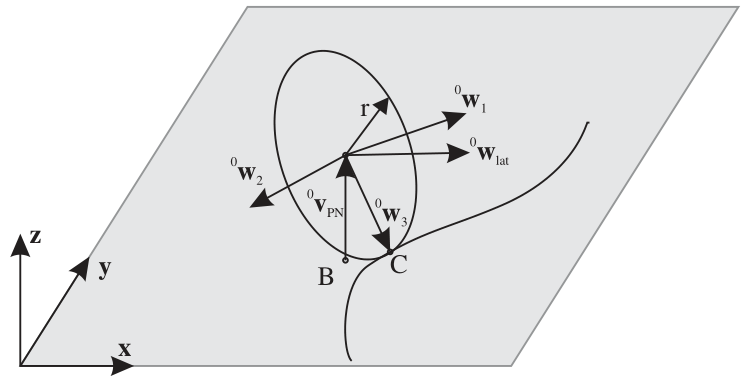
\includegraphics[height=4cm]{figures/ObjectJointRollingDiscSketch.pdf}
    \end{center}
    }
    First, the contact point $\LU{0}{\pv}_{C}$ must be computed.
    With the helper vector,
    \be
      \LU{0}{\xv} = \LU{0}{\wv}_1 \times \LU{0}{\vv_{PN}}
    \ee
    we obtain a disc coordinate system, representing the longitudinal direction,
    \be
      \LU{0}{\wv}_2 = \frac{1}{|\LU{0}{\xv}|} \LU{0}{\xv} 
    \ee
    and the vector to the contact point,
    \be
      \LU{0}{\wv}_3 = \LU{0}{\wv}_1 \times \LU{0}{\wv}_2
    \ee
    The contact point $C$ can be computed from
    \be
      \LU{0}{\pv}_{C} = \LU{0}{\pv}_{m1} + r \cdot \LU{0}{\wv}_3
    \ee
    The velocity of the contact point at the disc is computed from,
    \be
      \LU{0}{\vv}_{Cm1} = \LU{0}{\vv}_{m1} + \LU{0}{\tomega}_{m1} \times (r\cdot \LU{0}{\wv}_3)
    \ee
    If marker 0 body is (moving) rigid body instead of a ground body, the contact point $C$ is reconstructed in 
    body of marker 0,
    \be
      \LU{m0}{\pv}_{C} = \LU{m0,0}{\Rot} (\LU{0}{\pv}_{C} - \LU{0}{\pv}_{m0})
    \ee
    The velocity of the contact point at the marker 0 body reads
    \be
      \LU{0}{\vv}_{Cm0} = \LU{0}{\vv}_{m0} + \LU{0}{\tomega}_{m0} \times \left( \LU{0,m0}{\Rot} \LU{m0}{\pv}_{C} \right)
    \ee
    %
    \mysubsubsubsection{Connector constraint equations}
    \noindent Constraints for \texttt{activeConnector = True}:\\
    %
    The non-holonomic, index 2 constraints for the tangential and normal contact follow from (an index 3 formulation would be possible, but is not implemented yet because of mixing different jacobians)
    \be
      \LU{J1,0}{\Am} \left(\vr{\LU{0}{\vv}_{Cm1,x}}{\LU{0}{\vv}_{Cm1,y}}{\LU{0}{\vv}_{Cm1,z}} - \vr{\LU{0}{\vv}_{Cm0,x}}{\LU{0}{\vv}_{Cm0,y}}{\LU{0}{\vv}_{Cm0,z}} \right) = \Null
    \ee
    \noindent In case that \texttt{activeConnector = False}, the Lagrange multipliers are set to zero:
    \be
      \zv = \Null
    \ee
    Note that since version 1.8.27 the constraints can be turned on/off separately with \texttt{constrainedAxes=[b0,b1,b2]}, in which
    \texttt{b0} represents the flag for lateral motion, \texttt{b1} switches the constraint for forward motion and \texttt{b2} for motion in plane normal direction.
    %%RSTCOMPATIBLE
\vspace{6pt}\par\noindent\rule{\textwidth}{0.4pt}
%
\noindent For examples on ObjectJointRollingDisc see Relevant Examples and TestModels with weblink:
\bi
\item \exuUrl{https://github.com/jgerstmayr/EXUDYN/blob/master/main/pythonDev/Examples/bicycleIftommBenchmark.py}{\texttt{bicycleIftommBenchmark.py}} (Examples/)
\item \exuUrl{https://github.com/jgerstmayr/EXUDYN/blob/master/main/pythonDev/Examples/reinforcementLearningRobot.py}{\texttt{reinforcementLearningRobot.py}} (Examples/)
\item \exuUrl{https://github.com/jgerstmayr/EXUDYN/blob/master/main/pythonDev/TestModels/rollingCoinTest.py}{\texttt{rollingCoinTest.py}} (TestModels/)
\item \exuUrl{https://github.com/jgerstmayr/EXUDYN/blob/master/main/pythonDev/TestModels/rollingDiscTangentialForces.py}{\texttt{rollingDiscTangentialForces.py}} (TestModels/)
\item \exuUrl{https://github.com/jgerstmayr/EXUDYN/blob/master/main/pythonDev/TestModels/rotatingTableTest.py}{\texttt{rotatingTableTest.py}} (TestModels/)

\ei

%
\newpage

%+++++++++++++++++++++++++++++++++++

\mysubsubsection{ObjectJointRevolute2D}
\label{sec:item:ObjectJointRevolute2D}
A revolute joint in 2D; constrains the absolute 2D position of two points given by PointMarkers or RigidMarkers
\vspace{12pt}\\

\noindent \mybold{Additional information for ObjectJointRevolute2D}:
\bi
  \item This \texttt{Object} has/provides the following types = \texttt{Connector}, \texttt{Constraint}
  \item Requested \texttt{Marker} type = \texttt{Position}
  \item {\bf Short name} for Python = \texttt{RevoluteJoint2D}
  \item {\bf Short name} for Python visualization object = \texttt{VRevoluteJoint2D}
\ei\vspace{12pt} \noindent 
The item \mybold{ObjectJointRevolute2D} with type = 'JointRevolute2D' has the following parameters:
\vspace{-0.5cm}\\
\vspace{-0.5cm}\\
%reference manual TABLE
\begin{center}
  \footnotesize
  \begin{longtable}{| p{4.5cm} | p{2.5cm} | p{0.5cm} | p{2.5cm} | p{6cm} |}
    \hline
    \bf Name & \bf type & \bf size & \bf default value & \bf description \\ \hline
    name &     String &      &     '' &     constraints's unique name\\ \hline
    markerNumbers &     ArrayMarkerIndex &     \tabnewline  &     [ invalid [-1], invalid [-1] ] &     \tabnewline list of markers used in connector\\ \hline
    activeConnector &     Bool &      &     True &     flag, which determines, if the connector is active; used to deactivate (temporarily) a connector or constraint\\ \hline
    visualization &     VObjectJointRevolute2D &      &      &     parameters for visualization of item\\ \hline
\end{longtable}
\end{center}

\noindent The item VObjectJointRevolute2D has the following parameters:
%reference manual TABLE
\begin{center}
  \footnotesize
  \begin{longtable}{| p{4.5cm} | p{2.5cm} | p{0.5cm} | p{2.5cm} | p{6cm} |}
    \hline
    \bf Name & \bf type & \bf size & \bf default value & \bf description \\ \hline
    show &     Bool &      &     True &     set true, if item is shown in visualization and false if it is not shown\\ \hline
    drawSize &     float &      &     -1. &     drawing size = radius of revolute joint; size == -1.f means that default connector size is used\\ \hline
    color &     Float4 &      &     [-1.,-1.,-1.,-1.] &     \tabnewline RGBA connector color; if R==-1, use default color\\ \hline
\end{longtable}
\end{center}
\par\noindent\rule{\textwidth}{0.4pt}
\mysubsubsubsection{DESCRIPTION of ObjectJointRevolute2D:}
\label{description_ObjectJointRevolute2D}
\vspace{6pt}\par\noindent\rule{\textwidth}{0.4pt}
%
\noindent For examples on ObjectJointRevolute2D see Relevant Examples and TestModels with weblink:
\bi
\item \exuUrl{https://github.com/jgerstmayr/EXUDYN/blob/master/main/pythonDev/Examples/pendulumGeomExactBeam2D.py}{\texttt{pendulumGeomExactBeam2D.py}} (Examples/)
\item \exuUrl{https://github.com/jgerstmayr/EXUDYN/blob/master/main/pythonDev/Examples/sliderCrank3DwithANCFbeltDrive2.py}{\texttt{sliderCrank3DwithANCFbeltDrive2.py}} (Examples/)
\item \exuUrl{https://github.com/jgerstmayr/EXUDYN/blob/master/main/pythonDev/Examples/ANCFrotatingCable2D.py}{\texttt{ANCFrotatingCable2D.py}} (Examples/)
\item \exuUrl{https://github.com/jgerstmayr/EXUDYN/blob/master/main/pythonDev/Examples/ANCFslidingJoint2D.py}{\texttt{ANCFslidingJoint2D.py}} (Examples/)
\item \exuUrl{https://github.com/jgerstmayr/EXUDYN/blob/master/main/pythonDev/Examples/ANCFslidingJoint2Drigid.py}{\texttt{ANCFslidingJoint2Drigid.py}} (Examples/)
\item \exuUrl{https://github.com/jgerstmayr/EXUDYN/blob/master/main/pythonDev/Examples/beltDriveALE.py}{\texttt{beltDriveALE.py}} (Examples/)
\item \exuUrl{https://github.com/jgerstmayr/EXUDYN/blob/master/main/pythonDev/Examples/beltDriveReevingSystem.py}{\texttt{beltDriveReevingSystem.py}} (Examples/)
\item \exuUrl{https://github.com/jgerstmayr/EXUDYN/blob/master/main/pythonDev/Examples/beltDrivesComparison.py}{\texttt{beltDrivesComparison.py}} (Examples/)
\item \exuUrl{https://github.com/jgerstmayr/EXUDYN/blob/master/main/pythonDev/Examples/doublePendulum2D.py}{\texttt{doublePendulum2D.py}} (Examples/)
\item \exuUrl{https://github.com/jgerstmayr/EXUDYN/blob/master/main/pythonDev/Examples/finiteSegmentMethod.py}{\texttt{finiteSegmentMethod.py}} (Examples/)
\item \exuUrl{https://github.com/jgerstmayr/EXUDYN/blob/master/main/pythonDev/Examples/geneticOptimizationSliderCrank.py}{\texttt{geneticOptimizationSliderCrank.py}} (Examples/)
\item \exuUrl{https://github.com/jgerstmayr/EXUDYN/blob/master/main/pythonDev/Examples/HydraulicActuator2Arms.py}{\texttt{HydraulicActuator2Arms.py}} (Examples/)
\item  ...

\item \exuUrl{https://github.com/jgerstmayr/EXUDYN/blob/master/main/pythonDev/TestModels/ANCFbeltDrive.py}{\texttt{ANCFbeltDrive.py}} (TestModels/)
\item \exuUrl{https://github.com/jgerstmayr/EXUDYN/blob/master/main/pythonDev/TestModels/ANCFgeneralContactCircle.py}{\texttt{ANCFgeneralContactCircle.py}} (TestModels/)
\item \exuUrl{https://github.com/jgerstmayr/EXUDYN/blob/master/main/pythonDev/TestModels/ANCFoutputTest.py}{\texttt{ANCFoutputTest.py}} (TestModels/)
\item  ...


\ei

%
\newpage

%+++++++++++++++++++++++++++++++++++

\mysubsubsection{ObjectJointPrismatic2D}
\label{sec:item:ObjectJointPrismatic2D}
A prismatic joint in 2D; allows the relative motion of two bodies, using two RigidMarkers; the vector $\tv_0$ = axisMarker0 is given in local coordinates of the first marker's (body) frame and defines the prismatic axis; the vector $\mathbf{n}_1$ = normalMarker1 is given in the second marker's (body) frame and is the normal vector to the prismatic axis; using the global position vector $\pv_0$ and rotation matrix $\Am_0$ of marker0 and the global position vector $\pv_1$ rotation matrix $\Am_1$ of marker1, the equations for the prismatic joint follow as \be (\pv_1-\pv_0)^T\cdot \Am_1 \cdot \mathbf{n}_1 = 0 \ee  \be (\Am_0 \cdot \tv_0)^T \cdot \Am_1 \cdot \mathbf{n}_1 = 0\ee The lagrange multipliers follow for these two equations $[\lambda_0,\lambda_1]$, in which $\lambda_0$ is the transverse force and $\lambda_1$ is the torque in the joint.
\vspace{12pt}\\

\noindent \mybold{Additional information for ObjectJointPrismatic2D}:
\bi
  \item This \texttt{Object} has/provides the following types = \texttt{Connector}, \texttt{Constraint}
  \item Requested \texttt{Marker} type = \texttt{Position} + \texttt{Orientation}
  \item {\bf Short name} for Python = \texttt{PrismaticJoint2D}
  \item {\bf Short name} for Python visualization object = \texttt{VPrismaticJoint2D}
\ei\vspace{12pt} \noindent 
The item \mybold{ObjectJointPrismatic2D} with type = 'JointPrismatic2D' has the following parameters:
\vspace{-0.5cm}\\
\vspace{-0.5cm}\\
%reference manual TABLE
\begin{center}
  \footnotesize
  \begin{longtable}{| p{4.5cm} | p{2.5cm} | p{0.5cm} | p{2.5cm} | p{6cm} |}
    \hline
    \bf Name & \bf type & \bf size & \bf default value & \bf description \\ \hline
    name &     String &      &     '' &     constraints's unique name\\ \hline
    markerNumbers &     ArrayMarkerIndex &     \tabnewline  &     [ invalid [-1], invalid [-1] ] &     \tabnewline list of markers used in connector\\ \hline
    axisMarker0 &     Vector3D &      &     [1.,0.,0.] &     \tabnewline direction of prismatic axis, given as a 3D vector in Marker0 frame\\ \hline
    normalMarker1 &     Vector3D &      &     [0.,1.,0.] &     \tabnewline direction of normal to prismatic axis, given as a 3D vector in Marker1 frame\\ \hline
    constrainRotation &     Bool &      &     True &     flag, which determines, if the connector also constrains the relative rotation of the two objects; if set to false, the constraint will keep an algebraic equation set equal zero\\ \hline
    activeConnector &     Bool &      &     True &     flag, which determines, if the connector is active; used to deactivate (temporarily) a connector or constraint\\ \hline
    visualization &     VObjectJointPrismatic2D &      &      &     parameters for visualization of item\\ \hline
\end{longtable}
\end{center}

\noindent The item VObjectJointPrismatic2D has the following parameters:
%reference manual TABLE
\begin{center}
  \footnotesize
  \begin{longtable}{| p{4.5cm} | p{2.5cm} | p{0.5cm} | p{2.5cm} | p{6cm} |}
    \hline
    \bf Name & \bf type & \bf size & \bf default value & \bf description \\ \hline
    show &     Bool &      &     True &     set true, if item is shown in visualization and false if it is not shown\\ \hline
    drawSize &     float &      &     -1. &     drawing size = radius of revolute joint; size == -1.f means that default connector size is used\\ \hline
    color &     Float4 &      &     [-1.,-1.,-1.,-1.] &     \tabnewline RGBA connector color; if R==-1, use default color\\ \hline
\end{longtable}
\end{center}
\par\noindent\rule{\textwidth}{0.4pt}
\mysubsubsubsection{DESCRIPTION of ObjectJointPrismatic2D:}
\label{description_ObjectJointPrismatic2D}
\vspace{6pt}\par\noindent\rule{\textwidth}{0.4pt}
%
\noindent For examples on ObjectJointPrismatic2D see Relevant Examples and TestModels with weblink:
\bi
\item \exuUrl{https://github.com/jgerstmayr/EXUDYN/blob/master/main/pythonDev/Examples/sliderCrank3DwithANCFbeltDrive2.py}{\texttt{sliderCrank3DwithANCFbeltDrive2.py}} (Examples/)
\item \exuUrl{https://github.com/jgerstmayr/EXUDYN/blob/master/main/pythonDev/Examples/geneticOptimizationSliderCrank.py}{\texttt{geneticOptimizationSliderCrank.py}} (Examples/)
\item \exuUrl{https://github.com/jgerstmayr/EXUDYN/blob/master/main/pythonDev/TestModels/PARTS_ATEs_moving.py}{\texttt{PARTS\_ATEs\_moving.py}} (TestModels/)
\item \exuUrl{https://github.com/jgerstmayr/EXUDYN/blob/master/main/pythonDev/TestModels/scissorPrismaticRevolute2D.py}{\texttt{scissorPrismaticRevolute2D.py}} (TestModels/)
\item \exuUrl{https://github.com/jgerstmayr/EXUDYN/blob/master/main/pythonDev/TestModels/sliderCrankFloatingTest.py}{\texttt{sliderCrankFloatingTest.py}} (TestModels/)

\ei

%
\newpage

%+++++++++++++++++++++++++++++++++++

\mysubsubsection{ObjectJointSliding2D}
\label{sec:item:ObjectJointSliding2D}
A specialized sliding joint (without rotation) in 2D between a Cable2D (marker1) and a position-based marker (marker0); the data coordinate x[0] provides the current index in slidingMarkerNumbers, and x[1] the local position in the cable element at the beginning of the timestep.
\vspace{12pt}\\

\noindent \mybold{Additional information for ObjectJointSliding2D}:
\bi
  \item This \texttt{Object} has/provides the following types = \texttt{Connector}, \texttt{Constraint}
  \item Requested \texttt{Marker} type = \texttt{\_None}
  \item Requested \texttt{Node} type = \texttt{GenericData}
  \item {\bf Short name} for Python = \texttt{SlidingJoint2D}
  \item {\bf Short name} for Python visualization object = \texttt{VSlidingJoint2D}
\ei\vspace{12pt} \noindent 
The item \mybold{ObjectJointSliding2D} with type = 'JointSliding2D' has the following parameters:
\vspace{-0.5cm}\\
\vspace{-0.5cm}\\
%reference manual TABLE
\begin{center}
  \footnotesize
  \begin{longtable}{| p{4.5cm} | p{2.5cm} | p{0.5cm} | p{2.5cm} | p{6cm} |}
    \hline
    \bf Name & \bf type & \bf size & \bf default value & \bf description \\ \hline
    name &     String &      &     '' &     constraints's unique name\\ \hline
    markerNumbers &     ArrayMarkerIndex &     \tabnewline  &     [ invalid [-1], invalid [-1] ] &     \tabnewline marker m0: position or rigid body marker of mass point or rigid body; marker m1: updated marker to Cable2D element, where the sliding joint currently is attached to; must be initialized with an appropriate (global) marker number according to the starting position of the sliding object; this marker changes with time (PostNewtonStep)\\ \hline
    slidingMarkerNumbers &     ArrayMarkerIndex &     \tabnewline  &     [] &     these markers are used to update marker m1, if the sliding position exceeds the current cable's range; the markers must be sorted such that marker $m_{si}$ at x=cable(i).length is equal to marker(i+1) at x=0 of cable(i+1)\\ \hline
    slidingMarkerOffsets &     Vector &      &     [] &     this list contains the offsets of every sliding object (given by slidingMarkerNumbers) w.r.t. to the initial position (0): marker m0: offset=0, marker m1: offset=Length(cable0), marker m2: offset=Length(cable0)+Length(cable1), ...\\ \hline
    nodeNumber &     NodeIndex &      &     invalid (-1) &     \tabnewline node number of a NodeGenericData for 1 dataCoordinate showing the according marker number which is currently active and the start-of-step (global) sliding position\\ \hline
    classicalFormulation &     Bool &      &     True &     True: uses a formulation with 3 (+1) equations, including the force in sliding direction to be zero; forces in global coordinates, only index 3; False: use local formulation, which only needs 2 (+1) equations and can be used with index 2 formulation\\ \hline
    constrainRotation &     Bool &      &     False &     True: add constraint on rotation of marker m0 relative to slope (if True, marker m0 must be a rigid body marker); False: marker m0 body can rotate freely\\ \hline
    axialForce &     Real &      &     0 &     ONLY APPLIES if classicalFormulation==True; axialForce represents an additional sliding force acting between beam and marker m0 body in axial (beam) direction; this force can be used to drive a body on a beam, but can only be changed with user functions.\\ \hline
    activeConnector &     Bool &      &     True &     flag, which determines, if the connector is active; used to deactivate (temporarily) a connector or constraint\\ \hline
    visualization &     VObjectJointSliding2D &      &      &     parameters for visualization of item\\ \hline
\end{longtable}
\end{center}

\noindent The item VObjectJointSliding2D has the following parameters:
%reference manual TABLE
\begin{center}
  \footnotesize
  \begin{longtable}{| p{4.5cm} | p{2.5cm} | p{0.5cm} | p{2.5cm} | p{6cm} |}
    \hline
    \bf Name & \bf type & \bf size & \bf default value & \bf description \\ \hline
    show &     Bool &      &     True &     set true, if item is shown in visualization and false if it is not shown\\ \hline
    drawSize &     float &      &     -1. &     drawing size = radius of revolute joint; size == -1.f means that default connector size is used\\ \hline
    color &     Float4 &      &     [-1.,-1.,-1.,-1.] &     \tabnewline RGBA connector color; if R==-1, use default color\\ \hline
\end{longtable}
\end{center}
\par\noindent\rule{\textwidth}{0.4pt}
\mysubsubsubsection{DESCRIPTION of ObjectJointSliding2D:}
\label{description_ObjectJointSliding2D}
\paragraph{Information on input parameters:} 
\startTable{input parameter}{symbol}{description see tables above}
\rowTable{markerNumbers}{$[m0,m1]\tp$}{}
\rowTable{slidingMarkerNumbers}{$[m_{s0}, \ldots, m_{sn}]\tp$}{}
\rowTable{slidingMarkerOffsets}{$[d_{s0}, \ldots, d_{sn}]$}{}
\rowTable{nodeNumber}{$n_{GD}$}{}
\rowTable{axialForce}{$f_\mathrm{ax}$}{}
\finishTable

\mybold{The following output variables are available as OutputVariableType in sensors, Get...Output() and other functions}:
\begin{center}
\footnotesize
\begin{longtable}{| p{5cm} | p{5cm} | p{6cm} |} 
\hline
\bf output variable & \bf symbol & \bf description \\ \hline
Position &  & position vector of joint given by marker0\\ \hline
Velocity &  & velocity vector of joint given by marker0\\ \hline
SlidingCoordinate &  & global sliding coordinate along all elements; the maximum sliding coordinate is equivalent to the reference lengths of all sliding elements\\ \hline
Force &  & joint force vector (3D)\\ \hline
\end{longtable}
\end{center}
 \noindent
    \mysubsubsubsection{Definition of quantities}
    %\startTable{input parameter}{symbol}{description}
    %\rowTable{nodeNumber}{$n_{GD}$}{node number of generic data node}
    %\rowTable{markerNumbers[0]}{$m0$}{position-marker of mass point or rigid body (needs to be rigid body marker if constrainRotation==True)}
    %\rowTable{markerNumbers[1]}{$m1$}{marker to a Cable2D element, which is {\bf updated} in every PostNewtonStep; if the sliding body ($m0$) is in the range of all sliding cable elements, $m1$ contains the current marker number, which is active for the sliding joint}
    %\rowTable{slidingMarkerNumbers}{$[m_{s0}, \ldots, m_{sn}]\tp$}{a list of $sn$ (global) marker numbers which are are used to update marker1}
    %\rowTable{slidingMarkerOffsets}{$[d_{s0}, \ldots, d_{sn}]$}{a list of $sn$ scalar offsets, which represent the (reference arc) length of all previous sliding cable elements}
    %\finishTable
    %
    \startTable{intermediate variables}{symbol}{description}
    \rowTable{data node}{$\xv=[x_{data0},\,x_{data1}]\tp$}{coordinates of node with node number $n_{GD}$}
    \rowTable{data coordinate 0}{$x_{data0}$}{the current index in slidingMarkerNumbers}
    \rowTable{data coordinate 1}{$x_{data1}$}{the global sliding coordinate (ranging from 0 to the total length of all sliding elements) at {\bf start-of-step} - beginning of the timestep}
    \rowTable{marker m0 position}{$\LU{0}{\pv}_{m0}$}{current global position which is provided by marker m0}
    \rowTable{marker m0 velocity}{$\LU{0}{\vv}_{m0}$}{current global velocity which is provided by marker m0}
    %
    \rowTable{marker m0 orientation}{$\LU{0,m0}{\Rot}$}{current rotation matrix provided by marker m0 (assumed to be rigid body)}
    \rowTable{marker m0 angular velocity}{$\LU{0}{\tomega}_{m0}$}{current angular velocity vector provided by marker m0 (assumed to be rigid body)}
    %
    \rowTable{cable coordinates}{$\qv_{ANCF,m1}$}{current coordiantes of the ANCF cable element with the current marker $m1$ is referring to}
    \rowTable{sliding position}{$\LUR{0}{\rv}{ANCF} = \Sm(s_{el})\qv_{ANCF,m1}$}{current global position at the ANCF cable element, evaluated at local sliding position $s_{el}$}
    \rowTable{sliding position slope}{$\LURU{0}{\rv}{ANCF}{\prime} = \Sm^\prime(s_{el})\qv_{ANCF,m1} = [r^\prime_0,\,r^\prime_1]\tp$}{current global slope vector of the ANCF cable element, evaluated at local sliding position $s_{el}$}
    \rowTable{sliding velocity}{$\LUR{0}{\vv}{ANCF} = \Sm(s_{el})\dot\qv_{ANCF,m1}$}{current global velocity at the ANCF cable element, evaluated at local sliding position $s_{el}$ ($s_{el}$ not differentiated!!!)}
    \rowTable{sliding velocity slope}{$\LURU{0}{\vv}{ANCF}{\prime} = \Sm^\prime(s_{el})\dot\qv_{ANCF,m1}$}{current global slope velocity vector of the ANCF cable element, evaluated at local sliding position $s_{el}$}
    %
    \rowTable{sliding normal vector}{$\LU{0}{\nv} = [-r^\prime_1,\,r^\prime_0]$}{2D normal vector computed from slope $\rv^\prime=\LURU{0}{\rv}{ANCF}{\prime}$}
    \rowTable{sliding normal velocity vector}{$\LU{0}{\dot\nv} = [-\dot r^\prime_1,\,\dot r^\prime_0]$}{time derivative of 2D normal vector computed from slope velocity $\dot \rv^\prime=\LURU{0}{\dot \rv}{ANCF}{\prime}$}
    %
    \rowTable{algebraic coordinates}{$\zv=[\lambda_0,\,\lambda_1,\, s]\tp$}{algebraic coordinates composed of Lagrange multipliers $\lambda_0$ and $\lambda_1$ (in local cable coordinates: $\lambda_0$ is in axis direction) and the current sliding coordinate $s$, which is local in the current cable element. }
    \rowTable{local sliding coordinate}{$s$}{local incremental sliding coordinate $s$: the (algebraic) sliding coordinate {\bf relative to the start-of-step value}. Thus, $s$ only contains small local increments.}
    \finishTable
    \startTable{output variables}{symbol}{formula}
    \rowTable{Position}{$\LU{0}{\pv}_{m0}$}{current global position of position marker $m0$}
    \rowTable{Velocity}{$\LU{0}{\vv}_{m0}$}{current global velocity of position marker $m0$}
    \rowTable{SlidingCoordinate}{$s_g = s + x_{data1}$}{current value of the global sliding coordinate}
    \rowTable{Force}{$\fv$}{see below}
    \finishTable

    \mysubsubsubsection{Geometric relations}
    %cable
    Assume we have given the sliding coordinate $s$ (e.g., as a guess of the Newton method or beginning of the time step). 
    The element sliding coordinate (in the local coordinates of the current sliding element) is computed as
    \be
      s_{el} = s + x_{data1} - d_{m1} = s_g - d_{m1}.
    \ee
    The vector (=difference; error) between the marker $m0$ and the marker $m1$ (=$\rv_{ANCF}$) positions reads
    \be
      \LU{0}{\Delta\pv} = \LUR{0}{\rv}{ANCF} - \LU{0}{\pv}_{m0}
    \ee
    The vector (=difference; error) between the marker $m0$ and the marker $m1$ velocities reads
    \be
      \LU{0}{\Delta\vv} = \LUR{0}{\dot\rv}{ANCF} - \LU{0}{\vv}_{m0}
    \ee
    %
    %+++++++++++++++++++++++++++++++++++++++++++++
    \mysubsubsubsection{Connector constraint equations (classicalFormulation=True)}
    The 2D sliding joint is implemented having 3 equations (4 if constrainRotation==True, see below), using the special algebraic coordinates $\zv$.
    The algebraic equations read
    \bea
      \LU{0}{\Delta\pv} &=& \Null, \quad \mbox{... two index 3 eqs, ensure sliding body stays at cable}\\
      \left[\lambda_0,\lambda_1\right] \cdot  \LURU{0}{\rv}{ANCF}{\prime} - |\LURU{0}{\rv}{ANCF}{\prime}| \cdot f_\mathrm{ax} &=& 0, \quad \mbox{... one index 1 equ., 
                                               ensure force in sliding dir.~= 0}  \\
    \eea
    No index 2 case exists, because no time derivative exists for $s_{el}$. The jacobian matrices for algebraic and \hac{ODE2} coordinates read
    \be
      \Jm_{AE} = \mr{0}{0}{r^\prime_0} {0}{0}{r^\prime_1} {r^\prime_0}{r^\prime_1}{r^{\prime\prime}_0\lambda_0 + r^{\prime\prime}_1\lambda_1}    %\LURU{0}{\rv}{ANCF}{\prime\prime \mathrm{T}} \vp{\lambda_0}{\lambda_1}}
    \ee
    \be
      \Jm_{ODE2} = \mp{-J_{pos,m0}}{\Sm(s_{el})} {\Null\tp}{\left[\lambda_0,\,\lambda_1\right]\cdot\Sm^\prime(s_{el}) }
    \ee
    if \texttt{activeConnector = False}, the algebraic equations are changed to:
    \bea
      \lambda_0 &=& 0,   \\
      \lambda_1 &=& 0,   \\
      s &=& 0
    \eea
    %the algebraic variables are \be \qv_{AE}=[\lambda_x\;\; \lambda_y \;\; s]^T \ee in which $\lambda_x$ and $\lambda_y$ are the Lagrange multipliers for the position of the sliding joint; 
    %+++++++++++++++++++++++++++++++++++++++++++++
    \mysubsubsubsection{Connector constraint equations (classicalFormulation=False)}
    The 2D sliding joint is implemented having 3 equations (first equation is dummy and could be eliminated; 4 equations if constrainRotation==True, see below), using the special algebraic coordinates $\zv$. 
    The algebraic equations read
    \bea
      \lambda_0 &=& 0, \quad \mbox{... equation not necessary, but can be used for switching to other modes}  \\
      \LU{0}{\Delta\pv\tp} \LU{0}{\nv} &=& 0, \quad \mbox{... equation ensures that sliding body stays at cable centerline; index3}\\
      \LU{0}{\Delta\pv\tp} \LURU{0}{\rv}{ANCF}{\prime} &=& 0. \quad \mbox{... resolves the sliding coordinate $s$; index1 equation!}
    \eea
    In the index 2 case, the second equation reads
    \be
      \LU{0}{\Delta\vv\tp} \LU{0}{\nv}  + \LU{0}{\Delta\pv\tp} \LU{0}{\dot\nv}  = 0
    \ee
    if \texttt{activeConnector = False}, the algebraic equations are changed to:
    \bea
      \lambda_0 &=& 0,   \\
      \lambda_1 &=& 0,   \\
      s &=& 0
    \eea   
    %the algebraic variables are \be \qv_{AE}=[\lambda_x\;\; \lambda_y \;\; s]^T \ee in which $\lambda_x$ and $\lambda_y$ are the Lagrange multipliers for the position of the sliding joint; 
    %
    %+++++++++++++++++++++++++++++++++++++++++++++
    In case that \texttt{constrainRotation = True}, an additional constraint is added for the relative rotation
    between the slope of the cable and the orientation of marker m0 body.
    Assuming that the orientation of marker m0 is a 2D matrix (taking only $x$ and $y$ coordinates), the constraint reads
    \be
      \LURU{0}{\rv}{ANCF}{\prime\mathrm{T}} \LU{0,m0}{\Rot} \vp{0}{1} = 0
    \ee
    The index 2 case follows straightforward to 
    \be
      \LURU{0}{\dot \rv}{ANCF}{\prime\mathrm{T}} \LU{0,m0}{\Rot} \vp{0}{1}  + 
      \LURU{0}{\rv}{ANCF}{\prime\mathrm{T}} \LU{0,m0}{\Rot} \LU{0}{\tilde \tomega}_{m0} \vp{0}{1} = 0
    \ee
    again assuming, that $\LU{0}{\tilde \tomega}_{m0}$ is only a $2 \times 2$ matrix.
    %+++++++++++++++++++++++++++++++++++++++++++++
    \mysubsubsubsection{Post Newton Step}
    After the Newton solver has converged, a PostNewtonStep is performed for the element, which
    updates the marker $m1$ index if necessary.
    \bea
      s_{el} < 0 \quad \ra \quad x_{data0}\;-\!\!=1 \nonumber\\
      s_{el} > L \quad \ra \quad x_{data0}\;+\!\!=1
    \eea
    Furthermore, it is checked, if $x_{data0}$ becomes smaller than zero, which raises a warning and keeps $x_{data0}=0$.
    The same results if $x_{data0}\ge sn$, then $x_{data0} = sn$.
    Finally, the data coordinate is updated in order to provide the starting value for the next step,
    \be
      x_{data1} \;+\!\!= s.
    \ee
    %the data coordinates are \be \qv_{Data} = [i_{marker} \;\; s_{0}]^T \ee in which $i_{marker}$ is the current local index to the slidingMarkerNumber list and  $s_{0}$ is the sliding coordinate (which is the total sliding length along all cable elements in the cableMarkerNumber list) at the beginning of the solution step.
    %%RSTCOMPATIBLE
\vspace{6pt}\par\noindent\rule{\textwidth}{0.4pt}
%
\noindent For examples on ObjectJointSliding2D see Relevant Examples and TestModels with weblink:
\bi
\item \exuUrl{https://github.com/jgerstmayr/EXUDYN/blob/master/main/pythonDev/Examples/ANCFmovingRigidbody.py}{\texttt{ANCFmovingRigidbody.py}} (Examples/)
\item \exuUrl{https://github.com/jgerstmayr/EXUDYN/blob/master/main/pythonDev/Examples/ANCFslidingJoint2D.py}{\texttt{ANCFslidingJoint2D.py}} (Examples/)
\item \exuUrl{https://github.com/jgerstmayr/EXUDYN/blob/master/main/pythonDev/Examples/ANCFslidingJoint2Drigid.py}{\texttt{ANCFslidingJoint2Drigid.py}} (Examples/)
\item \exuUrl{https://github.com/jgerstmayr/EXUDYN/blob/master/main/pythonDev/Examples/ANCFswitchingSlidingJoint2D.py}{\texttt{ANCFswitchingSlidingJoint2D.py}} (Examples/)
\item \exuUrl{https://github.com/jgerstmayr/EXUDYN/blob/master/main/pythonDev/TestModels/modelUnitTests.py}{\texttt{modelUnitTests.py}} (TestModels/)

\ei

%
\newpage

%+++++++++++++++++++++++++++++++++++

\mysubsubsection{ObjectJointALEMoving2D}
\label{sec:item:ObjectJointALEMoving2D}
A specialized axially moving joint (without rotation) in 2D between a ALE Cable2D (marker1) and a position-based marker (marker0); ALE=Arbitrary Lagrangian Eulerian; the data coordinate x[0] provides the current index in slidingMarkerNumbers, and the \hac{ODE2} coordinate q[0] provides the (given) moving coordinate in the cable element.
\vspace{12pt}\\

\noindent \mybold{Additional information for ObjectJointALEMoving2D}:
\bi
  \item This \texttt{Object} has/provides the following types = \texttt{Connector}, \texttt{Constraint}
  \item Requested \texttt{Marker} type = \texttt{\_None}
  \item Requested \texttt{Node} type: read detailed information of item
  \item {\bf Short name} for Python = \texttt{ALEMovingJoint2D}
  \item {\bf Short name} for Python visualization object = \texttt{VALEMovingJoint2D}
\ei\vspace{12pt} \noindent 
The item \mybold{ObjectJointALEMoving2D} with type = 'JointALEMoving2D' has the following parameters:
\vspace{-0.5cm}\\
\vspace{-0.5cm}\\
%reference manual TABLE
\begin{center}
  \footnotesize
  \begin{longtable}{| p{4.5cm} | p{2.5cm} | p{0.5cm} | p{2.5cm} | p{6cm} |}
    \hline
    \bf Name & \bf type & \bf size & \bf default value & \bf description \\ \hline
    name &     String &      &     '' &     constraints's unique name\\ \hline
    markerNumbers &     ArrayMarkerIndex &     \tabnewline  &     [ invalid [-1], invalid [-1] ] &     \tabnewline marker m0: position-marker of mass point or rigid body; marker m1: updated marker to ANCF Cable2D element, where the sliding joint currently is attached to; must be initialized with an appropriate (global) marker number according to the starting position of the sliding object; this marker changes with time (PostNewtonStep)\\ \hline
    slidingMarkerNumbers &     ArrayMarkerIndex &     \tabnewline  &     [] &     a list of sn (global) marker numbers which are are used to update marker1\\ \hline
    slidingMarkerOffsets &     Vector &      &     [] &     this list contains the offsets of every sliding object (given by slidingMarkerNumbers) w.r.t. to the initial position (0): marker0: offset=0, marker1: offset=Length(cable0), marker2: offset=Length(cable0)+Length(cable1), ...\\ \hline
    slidingOffset &     Real &      &     0. &     sliding offset list [SI:m]: a list of sn scalar offsets, which represent the (reference arc) length of all previous sliding cable elements\\ \hline
    nodeNumbers &     ArrayNodeIndex &      &     [ invalid [-1], invalid [-1] ] &     \tabnewline node number of NodeGenericData (GD) with one data coordinate and of NodeGenericODE2 (ALE) with one \hac{ODE2} coordinate\\ \hline
    usePenaltyFormulation &     Bool &      &     False &     flag, which determines, if the connector is formulated with penalty, but still using algebraic equations (IsPenaltyConnector() still false)\\ \hline
    penaltyStiffness &     Real &      &     0. &     penalty stiffness [SI:N/m] used if usePenaltyFormulation=True\\ \hline
    activeConnector &     Bool &      &     True &     flag, which determines, if the connector is active; used to deactivate (temporarily) a connector or constraint\\ \hline
    visualization &     VObjectJointALEMoving2D &      &      &     parameters for visualization of item\\ \hline
\end{longtable}
\end{center}

\noindent The item VObjectJointALEMoving2D has the following parameters:
%reference manual TABLE
\begin{center}
  \footnotesize
  \begin{longtable}{| p{4.5cm} | p{2.5cm} | p{0.5cm} | p{2.5cm} | p{6cm} |}
    \hline
    \bf Name & \bf type & \bf size & \bf default value & \bf description \\ \hline
    show &     Bool &      &     True &     set true, if item is shown in visualization and false if it is not shown\\ \hline
    drawSize &     float &      &     -1. &     drawing size = radius of revolute joint; size == -1.f means that default connector size is used\\ \hline
    color &     Float4 &      &     [-1.,-1.,-1.,-1.] &     \tabnewline RGBA connector color; if R==-1, use default color\\ \hline
\end{longtable}
\end{center}
\par\noindent\rule{\textwidth}{0.4pt}
\mysubsubsubsection{DESCRIPTION of ObjectJointALEMoving2D:}
\label{description_ObjectJointALEMoving2D}
\paragraph{Information on input parameters:} 
\startTable{input parameter}{symbol}{description see tables above}
\rowTable{markerNumbers}{$[m0,\,m1]\tp$}{}
\rowTable{slidingMarkerNumbers}{$[m_{s0}, \ldots, m_{sn}]\tp$}{}
\rowTable{slidingMarkerOffsets}{$[d_{s0}, \ldots, d_{sn}]$}{}
\rowTable{slidingOffset}{$s_{off}$}{}
\rowTable{nodeNumbers}{$[n_{GD}, n_{ALE}]$}{}
\rowTable{penaltyStiffness}{$k$}{}
\finishTable

\mybold{The following output variables are available as OutputVariableType in sensors, Get...Output() and other functions}:
\begin{center}
\footnotesize
\begin{longtable}{| p{5cm} | p{5cm} | p{6cm} |} 
\hline
\bf output variable & \bf symbol & \bf description \\ \hline
Position & $\LU{0}{\pv}_{m0}$ & current global position of position marker $m0$\\ \hline
Velocity & $\LU{0}{\vv}_{m0}$ & current global velocity of position marker $m0$\\ \hline
SlidingCoordinate & $s_g = q_{ALE} + s_{off}$ & current value of the global sliding ALE coordinate, including offset; note that reference coordinate of $q_{ALE}$ is ignored!\\ \hline
Coordinates & $[x_{data0},\,q_{ALE}]\tp$ & provides two values: [0] = current sliding marker index, [1] = ALE sliding coordinate\\ \hline
Coordinates\_t & $[\dot q_{ALE}]\tp$ & provides ALE sliding velocity\\ \hline
Force & $\fv$ & joint force vector (3D)\\ \hline
\end{longtable}
\end{center}
 \noindent
    \mysubsubsubsection{Definition of quantities}
    %
    \startTable{intermediate variables}{symbol}{description}
    \rowTable{generic data node}{$\xv=[x_{data0}]\tp$}{coordinates of node with node number $n_{GD}$}
    \rowTable{generic \hac{ODE2} node}{$\qv=[q_{0}]\tp$}{coordinates of node with node number $n_{ALE}$, which is shared with all ALE-ANCF and ALE sliding joint objects}
    \rowTable{data coordinate}{$x_{data0}$}{the current index in slidingMarkerNumbers}
    \rowTable{ALE coordinate}{$q_{ALE} = q_{0}$}{current ALE coordinate (in fact this is the Eulerian coordinate in the ALE formulation); note that reference coordinate of $q_{ALE}$ is ignored!}
    \rowTable{marker m0 position}{$\LU{0}{\pv}_{m0}$}{current global position which is provided by marker m0}
    \rowTable{marker m0 velocity}{$\LU{0}{\vv}_{m0}$}{current global velocity which is provided by marker m0}
    %
    \rowTable{cable coordinates}{$\qv_{ANCF,m1}$}{current coordiantes of the ANCF cable element with the current marker $m1$ is referring to}
    \rowTable{sliding position}{$\LUR{0}{\rv}{ANCF} = \Sm(s_{el})\qv_{ANCF,m1}$}{current global position at the ANCF cable element, evaluated at local sliding position $s_{el}$}
    \rowTable{sliding position slope}{$\LURU{0}{\rv}{ANCF}{\prime} = \Sm^\prime(s_{el})\qv_{ANCF,m1}$}{current global slope vector of the ANCF cable element, evaluated at local sliding position $s_{el}$}
    \rowTable{sliding velocity}{$\LUR{0}{\vv}{ANCF} = \Sm(s_{el})\dot\qv_{ANCF,m1} + \dot q_{ALE} \LURU{0}{\rv}{ANCF}{\prime}$}{current global velocity at the ANCF cable element, evaluated at local sliding position $s_{el}$, including convective term}
    %
    \rowTable{sliding normal vector}{$\LU{0}{\nv} = [-r^\prime_1,\,r^\prime_0]$}{2D normal vector computed from slope $\rv^\prime=\LURU{0}{\rv}{ANCF}{\prime}$}
    %\rowTable{sliding normal vector}{$\LU{0}{\dot\nv} = [-\dot r^\prime_1,\,\dot r^\prime_0]$}{time derivative of 2D normal vector computed from slope velocity $\dot \rv^\prime=\LURU{0}{\dot \rv}{ANCF}{\prime}$}
    %
    \rowTable{algebraic variables}{$\zv=[\lambda_0,\,\lambda_1]\tp$}{algebraic variables (Lagrange multipliers) according to the algebraic equations }
    \finishTable
    %\startTable{output variables}{symbol}{formula}
    %\rowTable{Position}{$\LU{0}{\pv}_{m0}$}{current global position of position marker $m0$}
    %\rowTable{Velocity}{$\LU{0}{\vv}_{m0}$}{current global velocity of position marker $m0$}
    %\rowTable{SlidingCoordinate}{$s_g = q_{ALE} + s_{off}$}{current value of the global sliding ALE coordinate, including offset; note that reference coordinate of $q_{ALE}$ is ignored!}
    %\rowTable{Coordinates}{$[x_{data0},\,q_{ALE}]\tp$}{}
    %\rowTable{Coordinates\_t}{$[\dot q_{ALE}]\tp$}{}
    %\rowTable{Force}{$\fv$}{see below}
    %\finishTable

    \mysubsubsubsection{Geometric relations}
    The element sliding coordinate (in the local coordinates of the current sliding element) is computed from the ALE coordinate
    \be
      s_{el} = q_{ALE} + s_{off} - d_{m1} = s_g - d_{m1}.
    \ee
    For the description of the according quantities, see the description above. The distance $d_{m1}$ is obtained from the \texttt{slidingMarkerOffsets} list, using the current (local) index $x_{data0}$.
    The vector (=difference; error) between the marker $m0$ and the marker $m1$ (=$\rv_{ANCF}$) positions reads
    \be
      \LU{0}{\Delta\pv} = \LUR{0}{\rv}{ANCF} - \LU{0}{\pv}_{m0}
    \ee
    Note that $\LU{0}{\pv}_{m0}$ represents the current position of the marker $m0$, which could represent the midpoint of a mass sliding along the beam.
    The position $\LUR{0}{\rv}{ANCF}$ is computed from the beam represented by marker $m1$, using the local beam coordinate $x=s_{el}$. 
    The marker and the according beam finite element changes during movement using the list \texttt{slidingMarkerNumbers} and the index is updated in the PostNewtonStep.
    The vector (=difference; error) between the marker $m0$ and the marker $m1$ velocities reads
    \be
      \LU{0}{\Delta\vv} = \LUR{0}{\vv}{ANCF} - \LU{0}{\vv}_{m0}
    \ee
    %
    \ignoreRST{
    \begin{figure}[tbh]
        \label{fig:ObjectJointALEmoving2D}
        \begin{center}
            \includegraphics[height=4cm]{figures/ObjectJointALEmoving2D.pdf}
        \end{center}
        \caption{Geometrical relations for ALE sliding joint.}
    \end{figure}
    }
    %+++++++++++++++++++++++++++++++++++++++++++++
    \mysubsubsubsection{Connector constraint equations}
    The 2D sliding joint is implemented having 2 equations, using the Lagrange multipliers $\zv$. 
    The algebraic (index 3) equations read
    \be
      \LU{0}{\Delta\pv} = 0
    \ee
    Note that the Lagrange multipliers $[\lambda_0,\,\lambda_1]\tp$are the global forces in the joint.
    In the index 2 case the algebraic equations read
    \be
      \LU{0}{\Delta\vv} = 0
    \ee
    If \texttt{usePenalty = True}, the algebraic equations are changed to:
    \be
      \LU{0}{\Delta \pv} - \frac 1 k \zv = 0.
    \ee
    %
    %not realized yet, because \hac{AE} Jacobian becomes involved:
    %If \texttt{usePenaltyFormulation = True}, the algebraic equations are changed to:
    %\bea
    %  k_1 \LURU{0}{\rv}{ANCF}{\prime \mathrm{T}}   \LU{0}{\Delta\pv} - \lambda_0 &=& 0, \nonumber \\
    %  k_2 \LU{0}{\nv\tp}   \LU{0}{\Delta\pv}  - \lambda_1 &=& 0.
    %\eea
    %Note that in this case, the Lagrange multipliers $[\lambda_0,\,\lambda_1]\tp$are the local ($m1$) forces in the joint.

    \noindent If \texttt{activeConnector = False}, the algebraic equations are changed to:
    \bea
      \lambda_0 &=& 0,   \\
      \lambda_1 &=& 0.
    \eea   
    %
    %+++++++++++++++++++++++++++++++++++++++++++++
    \mysubsubsubsection{Post Newton Step}
    After the Newton solver has converged, a PostNewtonStep is performed for the element, which
    updates the marker $m1$ index if necessary.
    \bea
      s_{el} < 0 \quad \ra \quad x_{data0} \;-\!\!=1 \nonumber\\
      s_{el} > L \quad \ra \quad x_{data0} \;+\!\!=1
    \eea
    Furthermore, it is checked, if $x_{data0}$ becomes smaller than zero, which raises a warning and keeps $x_{data0}=0$.
    The same results if $x_{data0}\ge sn$, then $x_{data0} = sn$.
    Finally, the data coordinate is updated in order to provide the starting value for the next step,
    \be
      x_{data1} \;+\!\!= s.
    \ee
    %%RSTCOMPATIBLE
\vspace{6pt}\par\noindent\rule{\textwidth}{0.4pt}
%
\noindent For examples on ObjectJointALEMoving2D see Relevant Examples and TestModels with weblink:
\bi
\item \exuUrl{https://github.com/jgerstmayr/EXUDYN/blob/master/main/pythonDev/Examples/ANCFmovingRigidbody.py}{\texttt{ANCFmovingRigidbody.py}} (Examples/)
\item \exuUrl{https://github.com/jgerstmayr/EXUDYN/blob/master/main/pythonDev/TestModels/ANCFmovingRigidBodyTest.py}{\texttt{ANCFmovingRigidBodyTest.py}} (TestModels/)

\ei

%

\newpage
%+++++++++++++++++++++++++++++++
%+++++++++++++++++++++++++++++++
\mysubsection{Objects (Connector)}
A Connector is a special Object, which links two or more markers. A Connector which is not a Constraint, is a force element (e.g., spring-damper) or a penalty based joint.
%++++++

%+++++++++++++++++++++++++++++++++++

\mysubsubsection{ObjectConnectorSpringDamper}
\label{sec:item:ObjectConnectorSpringDamper}
An simple spring-damper element with additional force; connects to position-based markers.
\vspace{12pt}\\

\noindent \mybold{Additional information for ObjectConnectorSpringDamper}:
\bi
  \item This \texttt{Object} has/provides the following types = \texttt{Connector}
  \item Requested \texttt{Marker} type = \texttt{Position}
  \item {\bf Short name} for Python = \texttt{SpringDamper}
  \item {\bf Short name} for Python visualization object = \texttt{VSpringDamper}
\ei\vspace{12pt} \noindent 
The item \mybold{ObjectConnectorSpringDamper} with type = 'ConnectorSpringDamper' has the following parameters:
\vspace{-0.5cm}\\
\vspace{-0.5cm}\\
%reference manual TABLE
\begin{center}
  \footnotesize
  \begin{longtable}{| p{4.5cm} | p{2.5cm} | p{0.5cm} | p{2.5cm} | p{6cm} |}
    \hline
    \bf Name & \bf type & \bf size & \bf default value & \bf description \\ \hline
    name &     String &      &     '' &     connector's unique name\\ \hline
    markerNumbers &     ArrayMarkerIndex &     \tabnewline  &     [ invalid [-1], invalid [-1] ] &     \tabnewline list of markers used in connector\\ \hline
    referenceLength &     UReal &      &     0. &     reference length [SI:m] of spring\\ \hline
    stiffness &     UReal &      &     0. &     stiffness [SI:N/m] of spring; force acts against (length-initialLength)\\ \hline
    damping &     UReal &      &     0. &     damping [SI:N/(m s)] of damper; force acts against d/dt(length)\\ \hline
    force &     Real &      &     0. &     added constant force [SI:N] of spring; scalar force; f=1 is equivalent to reducing initialLength by 1/stiffness; f > 0: tension; f < 0: compression; can be used to model actuator force\\ \hline
    velocityOffset &     Real &      &     0. &     velocity offset [SI:m/s] of damper, being equivalent to time change of reference length\\ \hline
    activeConnector &     Bool &      &     True &     flag, which determines, if the connector is active; used to deactivate (temporarily) a connector or constraint\\ \hline
    springForceUserFunction &     PyFunctionMbsScalarIndexScalar5 &     \tabnewline  &     \tabnewline 0 &     A Python function which defines the spring force with parameters; the Python function will only be evaluated, if activeConnector is true, otherwise the SpringDamper is inactive; see description below\\ \hline
    visualization &     VObjectConnectorSpringDamper &      &      &     parameters for visualization of item\\ \hline
\end{longtable}
\end{center}

\noindent The item VObjectConnectorSpringDamper has the following parameters:
%reference manual TABLE
\begin{center}
  \footnotesize
  \begin{longtable}{| p{4.5cm} | p{2.5cm} | p{0.5cm} | p{2.5cm} | p{6cm} |}
    \hline
    \bf Name & \bf type & \bf size & \bf default value & \bf description \\ \hline
    show &     Bool &      &     True &     set true, if item is shown in visualization and false if it is not shown\\ \hline
    drawSize &     float &      &     -1. &     drawing size = diameter of spring; size == -1.f means that default connector size is used\\ \hline
    color &     Float4 &      &     [-1.,-1.,-1.,-1.] &     \tabnewline RGBA connector color; if R==-1, use default color\\ \hline
\end{longtable}
\end{center}
\par\noindent\rule{\textwidth}{0.4pt}
\mysubsubsubsection{DESCRIPTION of ObjectConnectorSpringDamper:}
\label{description_ObjectConnectorSpringDamper}
\paragraph{Information on input parameters:} 
\startTable{input parameter}{symbol}{description see tables above}
\rowTable{markerNumbers}{$[m0,m1]\tp$}{}
\rowTable{referenceLength}{$L_0$}{}
\rowTable{stiffness}{$k$}{}
\rowTable{damping}{$d$}{}
\rowTable{force}{$f_{a}$}{}
\rowTable{velocityOffset}{$\dot L_0$}{}
\rowTable{springForceUserFunction}{$\mathrm{UF} \in \Rcal$}{}
\finishTable

\mybold{The following output variables are available as OutputVariableType in sensors, Get...Output() and other functions}:
\begin{center}
\footnotesize
\begin{longtable}{| p{5cm} | p{5cm} | p{6cm} |} 
\hline
\bf output variable & \bf symbol & \bf description \\ \hline
Distance &  & distance between both points\\ \hline
Displacement &  & relative displacement between both points\\ \hline
Velocity &  & relative velocity between both points\\ \hline
Force & $\fv$ & 3D spring-damper force vector\\ \hline
ForceLocal & $f_{SD}$ & scalar spring-damper force\\ \hline
\end{longtable}
\end{center}
 \noindent
    \mysubsubsubsection{Definition of quantities}
    \startTable{intermediate variables}{symbol}{description}
    \rowTable{marker m0 position}{$\LU{0}{\pv}_{m0}$}{current global position which is provided by marker m0}
    \rowTable{marker m1 position}{$\LU{0}{\pv}_{m1}$}{}
    \rowTable{marker m0 velocity}{$\LU{0}{\vv}_{m0}$}{current global velocity which is provided by marker m0}
    \rowTable{marker m1 velocity}{$\LU{0}{\vv}_{m1}$}{}
    \rowTable{time derivative of distance}{$\dot L$}{$\Delta\! \LU{0}{\vv}\tp \vv_{f}$}
    \finishTable
    \startTable{output variables}{symbol}{formula}
    \rowTable{Displacement}{$\Delta\! \LU{0}{\pv}$}{$\LU{0}{\pv}_{m1} - \LU{0}{\pv}_{m0}$}
    \rowTable{Velocity}{$\Delta\! \LU{0}{\vv}$}{$\LU{0}{\vv}_{m1} - \LU{0}{\vv}_{m0}$}
    \rowTable{Distance}{$L$}{$|\Delta\! \LU{0}{\pv}|$}
    \rowTable{Force}{$\fv$}{see below}
    \finishTable
    %
    %++++++++++++++++++++++++++++++++++++++++++++++++++++++++++
    \mysubsubsubsection{Connector forces}
    %
    The unit vector in force direction reads (raises SysError if $L=0$),
    \be
      \vv_{f} = \frac{1}{L} \Delta\! \LU{0}{\pv}
    \ee
    If \texttt{activeConnector = True}, the scalar spring force is computed as
    \be
      f_{SD} = k\cdot(L-L_0) + d \cdot(\dot L -\dot L_0)+ f_{a}
    \ee
    If the springForceUserFunction $\mathrm{UF}$ is defined, $\fv$ instead becomes ($t$ is current time)
    \be
      f_{SD} = \mathrm{UF}(mbs, t, i_N, L-L_0, \dot L - \dot L_0, k, d, f_{a})
    \ee
    and \texttt{iN} represents the itemNumber (=objectNumber). Note that, if \texttt{activeConnector = False}, $f_{SD}$ is set to zero.

    The vector of the spring-damper force applied at both markers finally reads
    \be
      \fv = f_{SD}\vv_{f}
    \ee
    The virtual work of the connector force is computed from the virtual displacement 
    \be
      \delta \Delta\! \LU{0}{\pv} = \delta \LU{0}{\pv}_{m1} - \delta \LU{0}{\pv}_{m0} \eqComma
    \ee
    and the virtual work (note the transposed version here, because the resulting generalized forces shall be a column vector),
    \be
      \delta W_{SD} = \fv \delta \Delta\! \LU{0}{\pv} 
      = \left( k\cdot(L-L_0) + d \cdot (\dot L - \dot L_0) + f_{a} \right) \left(\delta \LU{0}{\pv}_{m1} - \delta \LU{0}{\pv}_{m0} \right)\tp \vv_{f} 
      \eqDot
    \ee
    The generalized (elastic) forces thus result from
    \be
      \Qm_{SD} = \frac{\partial \LU{0}{\pv}}{\partial \qv_{SD}\tp} \fv 
      \eqComma
    \ee
    and read for the markers $m0$ and $m1$,
    \be
      \Qm_{SD, m0} 
      = -\left( k\cdot(L-L_0) + d \cdot (\dot L - \dot L_0) + f_{a} \right) \Jm_{pos,m0}\tp \vv_{f} , \quad
      \Qm_{SD, m1} 
      = \left( k\cdot(L-L_0) + d \cdot (\dot L - \dot L_0)+ f_{a} \right) \Jm_{pos,m1}\tp \vv_{f} 
      \eqComma    
    \ee
    where $\Jm_{pos,m1}$ represents the derivative of marker $m1$ w.r.t.\ its associated coordinates $\qv_{m1}$, analogously $\Jm_{pos,m0}$.
    %
    \mysubsubsubsection{Connector Jacobian}
    The position-level jacobian for the connector, involving all coordinates associated with markers $m0$ and $m1$, follows from 
    \be
      \Jm_{SD} = \mp{\frac{\partial \Qm_{SD, m0}}{\partial \qv_{m0}} }{\frac{\partial \Qm_{SD, m0}}{\partial \qv_{m1}}}
                    {\frac{\partial \Qm_{SD, m0}}{\partial \qv_{m1}} }{\frac{\partial \Qm_{SD, m1}}{\partial \qv_{m1}}}
    \ee
    and the velocity level jacobian reads
    \be
      \Jm_{SD,t} = \mp{\frac{\partial \Qm_{SD, m0}}{\partial \dot \qv_{m0}} }{\frac{\partial \Qm_{SD, m0}}{\partial \dot \qv_{m1}}}
                    {\frac{\partial \Qm_{SD, m0}}{\partial \dot \qv_{m1}} }{\frac{\partial \Qm_{SD, m1}}{\partial \dot \qv_{m1}}}
    \ee
    The sub-Jacobians follow from
    \be
      \frac{\partial \Qm_{SD, m0}}{\partial \qv_{m0}} = 
       -\frac{\partial \Jm_{pos,m0}\tp }{\partial \qv_{m0}} \vv_{f} \left( k\cdot(L-L_0) + d \cdot(\dot L - \dot L_0) + f_{a} \right) 
       -\Jm_{pos,m0}\tp \frac{\partial \vv_{f} \left( k\cdot(L-L_0) + d \cdot(\dot L - \dot L_0) + f_{a} \right)   }{\partial \qv_{m0}} 
    \ee
    in which the term $\frac{\partial \Jm_{pos,m0}\tp }{\partial \qv_{m0}}$ is computed from a special function provided by markers, that
    compute the derivative of the marker jacobian times a constant vector, in this case the spring force $\fv$; this jacobian term is usually less  
    dominant, but is included in the numerical as well as the analytical derivatives, see the general jacobian computation information.
    
    The other term, which is the dominant term, is computed as (dependence of velocity term on position coordinates and $\dot L_0$ term neglected),
    \bea
      \frac{\partial \Qm_{SD, m0}}{\partial \qv_{m0}}
      &=& -\Jm_{pos,m0}\tp \frac{\partial \vv_{f} \left( k\cdot(L-L_0) + d \cdot(\dot L - \dot L_0) + f_{a} \right)   }{\partial \qv_{m0}}
      \nonumber \\
      &=& -\Jm_{pos,m0}\tp \frac{\partial  \left( k\cdot \left( \Delta\! \LU{0}{\pv} - L_0 \vv_{f} \right)+ \vv_{f} \left(d \cdot \vv_{f}\tp \Delta\! \LU{0}{\vv}  + f_{a} \right) \right)   }{\partial \qv_{m0}} 
      \nonumber \\
      &\approx& \Jm_{pos,m0}\tp \left(k\cdot \Im - k  \frac{L_0}{L}\left(\Im - \LU{0}{\vv_{f}} \otimes \LU{0}{\vv_{f}} \right)  +\frac{1}{L}\left(\Im - \LU{0}{\vv_{f}} \otimes \LU{0}{\vv_{f}} \right) \left(d \cdot \vv_{f}\tp \Delta\! \LU{0}{\vv}  + f_{a} \right) \right. \nonumber \\
      &&\left. + d \LU{0}{\vv_{f}} \otimes \left(\frac{1}{L}\left(\Im - \LU{0}{\vv_{f}} \otimes 
      \LU{0}{\vv_{f}} \right) \LU{0}{\vv_{f}} \right) \right)
      \LU{0}{\Jm_{pos,m0}}
    \eea
    %+++++++++++++++++++++++++++++++++++++++++++
    Alternatively (again $\dot L_0$ term neglected):
    \bea
      \frac{\partial \Qm_{SD, m0}}{\partial \qv_{m0}}
      &=& -\Jm_{pos,m0}\tp \frac{\partial \vv_{f} \left( k\cdot(L-L_0) + d \cdot(\dot L - \dot L_0) + f_{a} \right)   }{\partial \qv_{m0}}
      \nonumber \\
      %+++
      &=& \Jm_{pos,m0}\tp \frac{1}{L}\left(\Im - \LU{0}{\vv_{f}} \otimes \LU{0}{\vv_{f}} \right)
          \left( k\cdot(L-L_0) + d \cdot(\dot L - \dot L_0) + f_{a} \right) \Jm_{pos,m0}
      \nonumber \\
      && +\Jm_{pos,m0}\tp \LU{0}{\vv_{f}}
          \otimes \left( k\cdot \LU{0}{\vv_{f}} + d \cdot\Delta\! \LU{0}{\vv} \frac{1}{L}\left(\Im - \LU{0}{\vv_{f}} \otimes \LU{0}{\vv_{f}} \right) 
          \right) \Jm_{pos,m0} - d \Jm_{pos,m0}\tp \LU{0}{\vv_{f}} \otimes \LU{0}{\vv_{f}} \frac{\partial \Delta\! \LU{0}{\vv}}{\partial \qv_{m0}}  \nonumber \\
      %+++
      &=& \Jm_{pos,m0}\tp \left(\frac{f_{SD}}{L}\left(\Im - \LU{0}{\vv_{f}} \otimes \LU{0}{\vv_{f}} \right)
           + k \LU{0}{\vv_{f}} \otimes \LU{0}{\vv_{f}} + 
          \frac{d}{L} \left(\LU{0}{\vv_{f}} \otimes \Delta\! \LU{0}{\vv}\right) 
                 \cdot \left(\Im - \LU{0}{\vv_{f}} \otimes \LU{0}{\vv_{f}} \right) + ...!
          \right) \Jm_{pos,m0} 
    \eea
    %+++++++++++++++++++++++++++++++++++++++++++
    Noting that $\frac{\partial \vv_{f} }{\partial \qv_{m0}} = 
    -\frac{1}{L}\left(\Im - \LU{0}{\vv_{f}} \otimes \LU{0}{\vv_{f}} \right) \LU{0}{\Jm_{pos,m0}}$ and 
    $\frac{\partial \vv_{f} }{\partial \qv_{m1}} = 
    \frac{1}{L}\left(\Im - \LU{0}{\vv_{f}} \otimes \LU{0}{\vv_{f}} \right) \LU{0}{\Jm_{pos,m1}}$.
    %
    The Jacobian w.r.t.\ velocity coordinates follows as
    \bea
      \frac{\partial \Qm_{SD, m0}}{\partial \dot \qv_{m0}}
      &=& -\Jm_{pos,m0}\tp \frac{\partial \vv_{f} \left( k\cdot(L-L_0) + d \cdot(\dot L - \dot L_0) + f_{a} \right)   }{\partial \dot \qv_{m0}}
      \nonumber \\
      &=& \Jm_{pos,m0}\tp \left(d \vv_{f} \otimes \vv_{f} \right) \LU{0}{\Jm_{pos,m0}} 
    \eea
    Note that in case that $L=0$, the term $\frac{1}{L} \left(\Im - \LU{0}{\vv_{f}} \otimes \LU{0}{\vv_{f}} \right)$ is replaced
    by the unit matrix, in order to avoid zero (singular) jacobian; this is a workaround and should only occur in exceptional cases.
    
    The term $\frac{\partial \Delta\! \LU{0}{\vv}}{\partial \qv_{m0}}$, which is important for large damping, yields
    \be
      \frac{\partial \Delta\! \LU{0}{\vv}}{\partial \qv_{m0}} = 
      \frac{\partial \Jm_{pos,m0} \dot \qv_{m0}}{\partial \qv_{m0}}=
      \frac{\partial \Jm_{pos,m0} }{\partial \qv_{m0}} \dot \qv_{m0}
    \ee
    The latter term is currently neglected.
    
    Jacobians for markers $m1$ and mixed $m0$/$m1$ terms follow analogously.
    %++++++++++++++++++++++++++++++++++++++++++++++++++++++++++
    \userFunction{springForceUserFunction(mbs, t, itemNumber, deltaL, deltaL\_t, stiffness, damping, force)}
    A user function, which computes the spring force depending on time, object variables (deltaL, deltaL\_t) and 
    object parameters (stiffness, damping, force).
    The object variables are provided to the function using the current values of the SpringDamper object.
    Note that itemNumber represents the index of the object in mbs, which can be used to retrieve additional data from the object through
    \texttt{mbs.GetObjectParameter(itemNumber, ...)}, see the according description of \texttt{GetObjectParameter}.
    %
    \startTable{arguments /  return}{type or size}{description}
      \rowTable{\texttt{mbs}}{MainSystem}{provides MainSystem mbs to which object belongs}
      \rowTable{\texttt{t}}{Real}{current time in mbs}
      \rowTable{\texttt{itemNumber}}{Index}{integer number $i_N$ of the object in mbs, allowing easy access to all object data via mbs.GetObjectParameter(itemNumber, ...)}
      \rowTable{\texttt{deltaL}}{Real}{$L-L_0$, spring elongation}
      \rowTable{\texttt{deltaL\_t}}{Real}{$(\dot L - \dot L_0)$, spring velocity, including offset}
      \rowTable{\texttt{stiffness}}{Real}{copied from object}
      \rowTable{\texttt{damping}}{Real}{copied from object}
      \rowTable{\texttt{force}}{Real}{copied from object; constant force}
      \rowTable{\returnValue}{Real}{scalar value of computed spring force}
    \finishTable
    %
    %++++++++++++++++++++++++++++++++++++++++++++++++++++++++++
    \userFunctionExample{}
    \pythonstyle\begin{lstlisting}
        #define nonlinear force
        def UFforce(mbs, t, itemNumber, u, v, k, d, F0): 
            return k*u + d*v + F0
        #markerNumbers taken from mini example
        mbs.AddObject(ObjectConnectorSpringDamper(markerNumbers=[m0,m1],
                                                  referenceLength = 1, 
                                                  stiffness = 100, damping = 1,
                                                  springForceUserFunction = UFforce))
    \end{lstlisting} \vspace{12pt}
    %%RSTCOMPATIBLE
\vspace{6pt}\par\noindent\rule{\textwidth}{0.4pt}
\mysubsubsubsection{MINI EXAMPLE for ObjectConnectorSpringDamper}
\label{miniExample_ObjectConnectorSpringDamper}
\pythonstyle
\begin{lstlisting}[language=Python, firstnumber=1]
    node = mbs.AddNode(NodePoint(referenceCoordinates = [1.05,0,0]))
    oMassPoint = mbs.AddObject(MassPoint(nodeNumber = node, physicsMass=1))
    
    m0 = mbs.AddMarker(MarkerBodyPosition(bodyNumber=oGround, localPosition=[0,0,0]))
    m1 = mbs.AddMarker(MarkerBodyPosition(bodyNumber=oMassPoint, localPosition=[0,0,0]))
    
    mbs.AddObject(ObjectConnectorSpringDamper(markerNumbers=[m0,m1],
                                              referenceLength = 1, #shorter than initial distance
                                              stiffness = 100,
                                              damping = 1))

    #assemble and solve system for default parameters
    mbs.Assemble()
    mbs.SolveDynamic()

    #check result at default integration time
    exudynTestGlobals.testResult = mbs.GetNodeOutput(node, exu.OutputVariableType.Position)[0]
\end{lstlisting}

\vspace{6pt}\par\noindent\rule{\textwidth}{0.4pt}
%
\noindent For examples on ObjectConnectorSpringDamper see Relevant Examples and TestModels with weblink:
\bi
\item \exuUrl{https://github.com/jgerstmayr/EXUDYN/blob/master/main/pythonDev/Examples/HydraulicsUserFunction.py}{\texttt{HydraulicsUserFunction.py}} (Examples/)
\item \exuUrl{https://github.com/jgerstmayr/EXUDYN/blob/master/main/pythonDev/Examples/SpringDamperMassUserFunction.py}{\texttt{SpringDamperMassUserFunction.py}} (Examples/)
\item \exuUrl{https://github.com/jgerstmayr/EXUDYN/blob/master/main/pythonDev/Examples/ANCFcontactCircle.py}{\texttt{ANCFcontactCircle.py}} (Examples/)
\item \exuUrl{https://github.com/jgerstmayr/EXUDYN/blob/master/main/pythonDev/Examples/ANCFcontactCircle2.py}{\texttt{ANCFcontactCircle2.py}} (Examples/)
\item \exuUrl{https://github.com/jgerstmayr/EXUDYN/blob/master/main/pythonDev/Examples/ANCFslidingJoint2D.py}{\texttt{ANCFslidingJoint2D.py}} (Examples/)
\item \exuUrl{https://github.com/jgerstmayr/EXUDYN/blob/master/main/pythonDev/Examples/SpringWithConstraints.py}{\texttt{SpringWithConstraints.py}} (Examples/)
\item \exuUrl{https://github.com/jgerstmayr/EXUDYN/blob/master/main/pythonDev/Examples/stiffFlyballGovernor2.py}{\texttt{stiffFlyballGovernor2.py}} (Examples/)
\item \exuUrl{https://github.com/jgerstmayr/EXUDYN/blob/master/main/pythonDev/Examples/stiffFlyballGovernorKT.py}{\texttt{stiffFlyballGovernorKT.py}} (Examples/)
\item \exuUrl{https://github.com/jgerstmayr/EXUDYN/blob/master/main/pythonDev/TestModels/ANCFcontactCircleTest.py}{\texttt{ANCFcontactCircleTest.py}} (TestModels/)
\item \exuUrl{https://github.com/jgerstmayr/EXUDYN/blob/master/main/pythonDev/TestModels/modelUnitTests.py}{\texttt{modelUnitTests.py}} (TestModels/)
\item \exuUrl{https://github.com/jgerstmayr/EXUDYN/blob/master/main/pythonDev/TestModels/PARTS_ATEs_moving.py}{\texttt{PARTS\_ATEs\_moving.py}} (TestModels/)
\item \exuUrl{https://github.com/jgerstmayr/EXUDYN/blob/master/main/pythonDev/TestModels/stiffFlyballGovernor.py}{\texttt{stiffFlyballGovernor.py}} (TestModels/)

\ei

%
\newpage

%+++++++++++++++++++++++++++++++++++

\mysubsubsection{ObjectConnectorCartesianSpringDamper}
\label{sec:item:ObjectConnectorCartesianSpringDamper}
An 3D spring-damper element, providing springs and dampers in three (global) directions (x,y,z); the connector can be attached to position-based markers.
\vspace{12pt}\\

\noindent \mybold{Additional information for ObjectConnectorCartesianSpringDamper}:
\bi
  \item This \texttt{Object} has/provides the following types = \texttt{Connector}
  \item Requested \texttt{Marker} type = \texttt{Position}
  \item {\bf Short name} for Python = \texttt{CartesianSpringDamper}
  \item {\bf Short name} for Python visualization object = \texttt{VCartesianSpringDamper}
\ei\vspace{12pt} \noindent 
The item \mybold{ObjectConnectorCartesianSpringDamper} with type = 'ConnectorCartesianSpringDamper' has the following parameters:
\vspace{-0.5cm}\\
\vspace{-0.5cm}\\
%reference manual TABLE
\begin{center}
  \footnotesize
  \begin{longtable}{| p{4.5cm} | p{2.5cm} | p{0.5cm} | p{2.5cm} | p{6cm} |}
    \hline
    \bf Name & \bf type & \bf size & \bf default value & \bf description \\ \hline
    name &     String &      &     '' &     connector's unique name\\ \hline
    markerNumbers &     ArrayMarkerIndex &     \tabnewline  &     [ invalid [-1], invalid [-1] ] &     \tabnewline list of markers used in connector\\ \hline
    stiffness &     Vector3D &      &     [0.,0.,0.] &     \tabnewline stiffness [SI:N/m] of springs; act against relative displacements in 0, 1, and 2-direction\\ \hline
    damping &     Vector3D &      &     [0.,0.,0.] &     \tabnewline damping [SI:N/(m s)] of dampers; act against relative velocities in 0, 1, and 2-direction\\ \hline
    offset &     Vector3D &      &     [0.,0.,0.] &     \tabnewline offset between two springs\\ \hline
    springForceUserFunction &     PyFunctionVector3DmbsScalarIndexScalar4Vector3D &     \tabnewline  &     \tabnewline 0 &     \tabnewline A Python function which computes the 3D force vector between the two marker points, if activeConnector=True; see description below\\ \hline
    activeConnector &     Bool &      &     True &     flag, which determines, if the connector is active; used to deactivate (temporarily) a connector or constraint\\ \hline
    visualization &     VObjectConnectorCartesianSpringDamper &      &      &     parameters for visualization of item\\ \hline
\end{longtable}
\end{center}

\noindent The item VObjectConnectorCartesianSpringDamper has the following parameters:
%reference manual TABLE
\begin{center}
  \footnotesize
  \begin{longtable}{| p{4.5cm} | p{2.5cm} | p{0.5cm} | p{2.5cm} | p{6cm} |}
    \hline
    \bf Name & \bf type & \bf size & \bf default value & \bf description \\ \hline
    show &     Bool &      &     True &     set true, if item is shown in visualization and false if it is not shown\\ \hline
    drawSize &     float &      &     -1. &     drawing size = diameter of spring; size == -1.f means that default connector size is used\\ \hline
    color &     Float4 &      &     [-1.,-1.,-1.,-1.] &     \tabnewline RGBA connector color; if R==-1, use default color\\ \hline
\end{longtable}
\end{center}
\par\noindent\rule{\textwidth}{0.4pt}
\mysubsubsubsection{DESCRIPTION of ObjectConnectorCartesianSpringDamper:}
\label{description_ObjectConnectorCartesianSpringDamper}
\paragraph{Information on input parameters:} 
\startTable{input parameter}{symbol}{description see tables above}
\rowTable{markerNumbers}{$[m0,m1]\tp$}{}
\rowTable{stiffness}{$\kv$}{}
\rowTable{damping}{$\dv$}{}
\rowTable{offset}{$\vv_{\mathrm{off}}$}{}
\rowTable{springForceUserFunction}{$\mathrm{UF} \in \Rcal^3$}{}
\finishTable

\mybold{The following output variables are available as OutputVariableType in sensors, Get...Output() and other functions}:
\begin{center}
\footnotesize
\begin{longtable}{| p{5cm} | p{5cm} | p{6cm} |} 
\hline
\bf output variable & \bf symbol & \bf description \\ \hline
Displacement & $\Delta\! \LU{0}{\pv} = \LU{0}{\pv}_{m1} - \LU{0}{\pv}_{m0}$ & relative displacement in global coordinates\\ \hline
Distance & $L=|\Delta\! \LU{0}{\pv}|$ & scalar distance between both marker points\\ \hline
Velocity & $\Delta\! \LU{0}{\vv} = \LU{0}{\vv}_{m1} - \LU{0}{\vv}_{m0}$ & relative translational velocity in global coordinates\\ \hline
Force & $\fv_{SD}$ & joint force in global coordinates, see equations\\ \hline
\end{longtable}
\end{center}
 \noindent
    \mysubsubsubsection{Definition of quantities}
    \startTable{intermediate variables}{symbol}{description}
    \rowTable{marker m0 position}{$\LU{0}{\pv}_{m0}$}{current global position which is provided by marker m0}
    \rowTable{marker m1 position}{$\LU{0}{\pv}_{m1}$}{}
    \rowTable{marker m0 velocity}{$\LU{0}{\vv}_{m0}$}{current global velocity which is provided by marker m0}
    \rowTable{marker m1 velocity}{$\LU{0}{\vv}_{m1}$}{}
    \finishTable
    %+++++++++++++++++++++++++++++++++++++++++++++++++++
    \mysubsubsubsection{Connector forces}
    Connector forces are based on relative displacements and relative veolocities in global coordinates.
    Relative displacement between marker m0 to marker m1 positions is given by
    \be \label{eq_ObjectCartesianSpringDamper_deltaPos}
      \Delta\! \LU{0}{\pv}= \LU{0}{\pv}_{m1} - \LU{0}{\pv}_{m0} \eqComma
    \ee
    and relative velocity reads
    \be
      \Delta\! \LU{0}{\vv}= \LU{0}{\vv}_{m1} - \LU{0}{\vv}_{m0} \eqDot
    \ee
    If \texttt{activeConnector = True}, the spring force vector is computed as
    \be
      \LU{0}{\fv_{SD}} = \diag(\kv)\cdot(\Delta\! \LU{0}{\pv}-\LU{0}{\vv_{\mathrm{off}}}) + \diag(\dv) \cdot \Delta\! \LU{0}{\vv} \eqDot
    \ee
    If the springForceUserFunction $\mathrm{UF}$ is defined, $\fv_{SD}$ instead becomes ($t$ is current time)
    \be
      \LU{0}{\fv_{SD}} = \mathrm{UF}(mbs, t, i_N, \Delta\! \LU{0}{\pv}, \Delta\! \LU{0}{\vv}, \kv, \dv, \vv_{\mathrm{off}}) \eqComma
    \ee
    and \texttt{iN} represents the itemNumber (=objectNumber).
    If \texttt{activeConnector = False}, $\fv_{SD}$ is set to zero.
    %+++++++++++++++++++++++++++++++++++++++++++++++++++

    The force $\fv_{SD}$ acts via the markers' position jacobians $\Jm_{pos,m0}$ and $\Jm_{pos,m1}$.
    The generalized forces added to the \ac{LHS} equations read for marker $m0$,
    \be
      \fv_{LHS,m0} = -\LU{0}{\Jm_{pos,m0}\tp} \LU{0}{\fv_{SD}} \eqComma
    \ee
    and for marker $m1$,
    \be
      \fv_{LHS,m1} =  \LU{0}{\Jm_{pos,m1}\tp} \LU{0}{\fv_{SD}} \eqDot
    \ee
    The \ac{LHS} equation parts are added accordingly using the \ac{LTG} mapping.
    Note that the different signs result from the signs in \eq{eq_ObjectCartesianSpringDamper_deltaPos}.

    The connector also provides an analytic jacobian, which is used if \texttt{newton.numericalDifferentiation.forODE2 = False} 
    and if there is no springForceUserFunction (otherwise numerical differentiation is used).
    
    The anayltic jacobian for the coupled equation parts $\fv_{LHS,m0}$ and $\fv_{LHS,m1}$ is based on the local jacobians
    \bea
      \Jm_{loc0} &=& f_{ODE2}\frac{\partial \LU{0}{\fv_{SD}}}{\partial \LU{0}{\pv}_{m0}} +
                     f_{ODE2_t}\frac{\partial \LU{0}{\fv_{SD}}}{\partial \LU{0}{\vv}_{m0}}
                  = -f_{ODE2} \cdot \diag(\kv) - f_{ODE2_t} \cdot \diag(\dv) \eqComma \nonumber \\
      \Jm_{loc1} &=& f_{ODE2}\frac{\partial \LU{0}{\fv_{SD}}}{\partial \LU{0}{\pv}_{m1}} +
                     f_{ODE2_t}\frac{\partial \LU{0}{\fv_{SD}}}{\partial \LU{0}{\vv}_{m1}}
                  =  f_{ODE2} \cdot \diag(\kv) + f_{ODE2_t} \cdot \diag(\dv) \eqDot
    \eea
    Here, $f_{ODE2}$ is the factor for the position derivative and $f_{ODE2_t}$ is the factor for the velocity derivative, 
    which allows a computation of the computation for both the position as well as the velocity part at the same time.

    \noindent The complete jacobian for the \ac{LHS} equations then reads,
    \bea
      \Jm_{CSD}&=&\mp{\displaystyle \frac{\partial \fv_{LHS,m0}}{\partial  \qv_{m0}}}
                  {\displaystyle \frac{\partial \fv_{LHS,m0}}{\partial  \qv_{m1}}}
                  {\displaystyle \frac{\partial \fv_{LHS,m1}}{\partial  \qv_{m0}}}
                  {\displaystyle \frac{\partial \fv_{LHS,m1}}{\partial  \qv_{m1}}} + \Jm_{CSD'} \nonumber \\
            &=& \mp{-\LU{0}{\Jm_{pos,m0}\tp} \Jm_{loc0} \Jm_{pos,m0}}
                   {-\LU{0}{\Jm_{pos,m0}\tp} \Jm_{loc1} \Jm_{pos,m1}}
                   {\LU{0}{\Jm_{pos,m1}\tp} \Jm_{loc0} \Jm_{pos,m0}}
                   {\LU{0}{\Jm_{pos,m1}\tp} \Jm_{loc1} \Jm_{pos,m1}} + \Jm_{CSD'} \nonumber \\
            &=& \mp{\LU{0}{\Jm_{pos,m0}\tp} \Jm_{loc1} \Jm_{pos,m0}}
                   {-\LU{0}{\Jm_{pos,m0}\tp} \Jm_{loc1} \Jm_{pos,m1}}
                   {-\LU{0}{\Jm_{pos,m1}\tp} \Jm_{loc1} \Jm_{pos,m0}}
                   {\LU{0}{\Jm_{pos,m1}\tp} \Jm_{loc1} \Jm_{pos,m1}} + \Jm_{CSD'}
    \eea
    Here, $\qv_{m0}$ are the coordinates associated with marker $m0$ and $\qv_{m1}$ of marker $m1$.

    The second term $\Jm_{CSD'}$ is only non-zero if $\frac{\partial \LU{0}{\Jm_{pos,i}\tp}}{\partial \qv_{i}}$ is non-zero, using $i \in \{m0, \, m1\}$.
    As the latter terms would require to compute a 3-dimensional array, the second jacobian term is computed as 
    \be \label{eq_ObjectCartesianSpringDamper_jacDeriv}
      \Jm_{CSD'} = \mp{-f_{ODE2}\frac{\partial \left(\LU{0}{\Jm_{pos,m0}\tp} \fv' \right)}{\partial \qv_{m0}}}{\Null}{\Null}
                      { f_{ODE2}\frac{\partial \left(\LU{0}{\Jm_{pos,m1}\tp} \fv' \right)}{\partial \qv_{m1}}}
    \ee
    in which we set $\fv' = \LU{0}{\fv_{SD}}$, but the derivatives in \eq{eq_ObjectCartesianSpringDamper_jacDeriv} are evaluated by setting $\fv' = const$.

    %++++++++++++++++++++++++++++++++++++++++++++++++++++++++++
    \userFunction{springForceUserFunction(mbs, t, itemNumber, displacement, velocity, stiffness, damping, offset)}
    A user function, which computes the 3D spring force vector depending on time, object variables (deltaL, deltaL\_t) and object parameters 
    (stiffness, damping, force).
    The object variables are provided to the function using the current values of the SpringDamper object.
    Note that itemNumber represents the index of the object in mbs, which can be used to retrieve additional data from the object through
    \texttt{mbs.GetObjectParameter(itemNumber, ...)}, see the according description of \texttt{GetObjectParameter}.
    %
    \startTable{arguments / return}{type or size}{description}
      \rowTable{\texttt{mbs}}{MainSystem}{provides MainSystem mbs in which underlying item is defined}
      \rowTable{\texttt{t}}{Real}{current time in mbs} %use t instead time in order to avoid possible conflicts with Python time
      \rowTable{\texttt{itemNumber}}{Index}{integer number $i_N$ of the object in mbs, allowing easy access to all object data via mbs.GetObjectParameter(itemNumber, ...)}
      \rowTable{\texttt{displacement}}{Vector3D}{$\Delta\! \LU{0}{\pv}$}
      \rowTable{\texttt{velocity}}{Vector3D}{$\Delta\! \LU{0}{\vv}$}
      %
      \rowTable{\texttt{stiffness}}{Vector3D}{copied from object}
      \rowTable{\texttt{damping}}{Vector3D}{copied from object}
      \rowTable{\texttt{offset}}{Vector3D}{copied from object}
      \rowTable{\returnValue}{Vector3D}{list or numpy array of computed spring force}
    \finishTable
    %++++++++++++++++++++++++++++++++++++++++++++++++++++++++++
    \userFunctionExample{}
    \pythonstyle\begin{lstlisting}
        #define simple force for spring-damper:
        def UFforce(mbs, t, itemNumber, u, v, k, d, offset): 
            return [u[0]*k[0],u[1]*k[1],u[2]*k[2]]
        
        #markerNumbers and parameters taken from mini example
        mbs.AddObject(CartesianSpringDamper(markerNumbers = [mGround, mMass], 
                                            stiffness = [k,k,k], 
                                            damping = [0,k*0.05,0], offset = [0,0,0],
                                            springForceUserFunction = UFforce))
    \end{lstlisting}
    %%RSTCOMPATIBLE
\vspace{6pt}\par\noindent\rule{\textwidth}{0.4pt}
\mysubsubsubsection{MINI EXAMPLE for ObjectConnectorCartesianSpringDamper}
\label{miniExample_ObjectConnectorCartesianSpringDamper}
\pythonstyle
\begin{lstlisting}[language=Python, firstnumber=1]
    #example with mass at [1,1,0], 5kg under load 5N in -y direction
    k=5000
    nMass = mbs.AddNode(NodePoint(referenceCoordinates=[1,1,0]))
    oMass = mbs.AddObject(MassPoint(physicsMass = 5, nodeNumber = nMass))
    
    mMass = mbs.AddMarker(MarkerNodePosition(nodeNumber=nMass))
    mGround = mbs.AddMarker(MarkerBodyPosition(bodyNumber=oGround, localPosition = [1,1,0]))
    mbs.AddObject(CartesianSpringDamper(markerNumbers = [mGround, mMass], 
                                        stiffness = [k,k,k], 
                                        damping = [0,k*0.05,0], offset = [0,0,0]))
    mbs.AddLoad(Force(markerNumber = mMass, loadVector = [0, -5, 0])) #static solution=-5/5000=-0.001m

    #assemble and solve system for default parameters
    mbs.Assemble()
    mbs.SolveDynamic()

    #check result at default integration time
    exudynTestGlobals.testResult = mbs.GetNodeOutput(nMass, exu.OutputVariableType.Displacement)[1]
\end{lstlisting}

\vspace{6pt}\par\noindent\rule{\textwidth}{0.4pt}
%
\noindent For examples on ObjectConnectorCartesianSpringDamper see Relevant Examples and TestModels with weblink:
\bi
\item \exuUrl{https://github.com/jgerstmayr/EXUDYN/blob/master/main/pythonDev/Examples/mouseInteractionExample.py}{\texttt{mouseInteractionExample.py}} (Examples/)
\item \exuUrl{https://github.com/jgerstmayr/EXUDYN/blob/master/main/pythonDev/Examples/rigid3Dexample.py}{\texttt{rigid3Dexample.py}} (Examples/)
\item \exuUrl{https://github.com/jgerstmayr/EXUDYN/blob/master/main/pythonDev/Examples/sliderCrank3DwithANCFbeltDrive2.py}{\texttt{sliderCrank3DwithANCFbeltDrive2.py}} (Examples/)
\item \exuUrl{https://github.com/jgerstmayr/EXUDYN/blob/master/main/pythonDev/Examples/ANCFcontactCircle.py}{\texttt{ANCFcontactCircle.py}} (Examples/)
\item \exuUrl{https://github.com/jgerstmayr/EXUDYN/blob/master/main/pythonDev/Examples/ANCFcontactCircle2.py}{\texttt{ANCFcontactCircle2.py}} (Examples/)
\item \exuUrl{https://github.com/jgerstmayr/EXUDYN/blob/master/main/pythonDev/Examples/ANCFslidingJoint2D.py}{\texttt{ANCFslidingJoint2D.py}} (Examples/)
\item \exuUrl{https://github.com/jgerstmayr/EXUDYN/blob/master/main/pythonDev/Examples/flexibleRotor3Dtest.py}{\texttt{flexibleRotor3Dtest.py}} (Examples/)
\item \exuUrl{https://github.com/jgerstmayr/EXUDYN/blob/master/main/pythonDev/Examples/lavalRotor2Dtest.py}{\texttt{lavalRotor2Dtest.py}} (Examples/)
\item \exuUrl{https://github.com/jgerstmayr/EXUDYN/blob/master/main/pythonDev/Examples/NGsolvePistonEngine.py}{\texttt{NGsolvePistonEngine.py}} (Examples/)
\item \exuUrl{https://github.com/jgerstmayr/EXUDYN/blob/master/main/pythonDev/Examples/NGsolvePostProcessingStresses.py}{\texttt{NGsolvePostProcessingStresses.py}} (Examples/)
\item \exuUrl{https://github.com/jgerstmayr/EXUDYN/blob/master/main/pythonDev/Examples/objectFFRFreducedOrderNetgen.py}{\texttt{objectFFRFreducedOrderNetgen.py}} (Examples/)
\item \exuUrl{https://github.com/jgerstmayr/EXUDYN/blob/master/main/pythonDev/Examples/particlesTest3D.py}{\texttt{particlesTest3D.py}} (Examples/)
\item  ...

\item \exuUrl{https://github.com/jgerstmayr/EXUDYN/blob/master/main/pythonDev/TestModels/scissorPrismaticRevolute2D.py}{\texttt{scissorPrismaticRevolute2D.py}} (TestModels/)
\item \exuUrl{https://github.com/jgerstmayr/EXUDYN/blob/master/main/pythonDev/TestModels/sphericalJointTest.py}{\texttt{sphericalJointTest.py}} (TestModels/)
\item \exuUrl{https://github.com/jgerstmayr/EXUDYN/blob/master/main/pythonDev/TestModels/ANCFcontactCircleTest.py}{\texttt{ANCFcontactCircleTest.py}} (TestModels/)
\item  ...


\ei

%
\newpage

%+++++++++++++++++++++++++++++++++++

\mysubsubsection{ObjectConnectorRigidBodySpringDamper}
\label{sec:item:ObjectConnectorRigidBodySpringDamper}
An 3D spring-damper element acting on relative displacements and relative rotations of two rigid body (position+orientation) markers; connects to (position+orientation)-based markers and represents a penalty-based rigid joint (or prismatic, revolute, etc.)
\vspace{12pt}\\

\noindent \mybold{Additional information for ObjectConnectorRigidBodySpringDamper}:
\bi
  \item This \texttt{Object} has/provides the following types = \texttt{Connector}
  \item Requested \texttt{Marker} type = \texttt{Position} + \texttt{Orientation}
  \item Requested \texttt{Node} type = \texttt{GenericData}
  \item {\bf Short name} for Python = \texttt{RigidBodySpringDamper}
  \item {\bf Short name} for Python visualization object = \texttt{VRigidBodySpringDamper}
\ei\vspace{12pt} \noindent 
The item \mybold{ObjectConnectorRigidBodySpringDamper} with type = 'ConnectorRigidBodySpringDamper' has the following parameters:
\vspace{-0.5cm}\\
\vspace{-0.5cm}\\
%reference manual TABLE
\begin{center}
  \footnotesize
  \begin{longtable}{| p{4.5cm} | p{2.5cm} | p{0.5cm} | p{2.5cm} | p{6cm} |}
    \hline
    \bf Name & \bf type & \bf size & \bf default value & \bf description \\ \hline
    name &     String &      &     '' &     connector's unique name\\ \hline
    markerNumbers &     ArrayMarkerIndex &     \tabnewline  &     [ invalid [-1], invalid [-1] ] &     \tabnewline list of markers used in connector\\ \hline
    nodeNumber &     NodeIndex &      &     invalid (-1) &     \tabnewline node number of a NodeGenericData (size depends on application) for dataCoordinates for user functions (e.g., implementing contact/friction user function)\\ \hline
    stiffness &     Matrix6D &      &     np.zeros((6,6)) &     stiffness [SI:N/m or Nm/rad] of translational, torsional and coupled springs; act against relative displacements in x, y, and z-direction as well as the relative angles (calculated as Euler angles); in the simplest case, the first 3 diagonal values correspond to the local stiffness in x,y,z direction and the last 3 diagonal values correspond to the rotational stiffness around x,y and z axis\\ \hline
    damping &     Matrix6D &      &     np.zeros((6,6)) &     damping [SI:N/(m/s) or Nm/(rad/s)] of translational, torsional and coupled dampers; very similar to stiffness, however, the rotational velocity is computed from the angular velocity vector\\ \hline
    rotationMarker0 &     Matrix3D &      &     [[1,0,0], [0,1,0], [0,0,1]] &     \tabnewline local rotation matrix for marker 0; stiffness, damping, etc. components are measured in local coordinates relative to rotationMarker0\\ \hline
    rotationMarker1 &     Matrix3D &      &     [[1,0,0], [0,1,0], [0,0,1]] &     \tabnewline local rotation matrix for marker 1; stiffness, damping, etc. components are measured in local coordinates relative to rotationMarker1\\ \hline
    offset &     Vector6D &      &     [0.,0.,0.,0.,0.,0.] &     \tabnewline translational and rotational offset considered in the spring force calculation\\ \hline
    intrinsicFormulation &     Bool &      &     False &     if True, the joint uses the intrinsic formulation, which is independent on order of markers, using a mid-point and mid-rotation for evaluation and application of connector forces and torques; this uses a Lie group formulation; in this case, the force/torque vector is computed from the stiffness matrix times the 6-vector of the SE3 matrix logarithm between the two marker positions/rotations, see the equations\\ \hline
    activeConnector &     Bool &      &     True &     flag, which determines, if the connector is active; used to deactivate (temporarily) a connector or constraint\\ \hline
    springForceTorqueUserFunction &     PyFunctionVector6DmbsScalarIndex4Vector3D2Matrix6D2Matrix3DVector6D &     \tabnewline  &     \tabnewline 0 &     \tabnewline A Python function which computes the 6D force-torque vector (3D force + 3D torque) between the two rigid body markers, if activeConnector=True; see description below\\ \hline
    postNewtonStepUserFunction &     PyFunctionVectorMbsScalarIndex4VectorVector3D2Matrix6D2Matrix3DVector6D &     \tabnewline  &     \tabnewline 0 &     \tabnewline A Python function which computes the error of the PostNewtonStep; see description below\\ \hline
    visualization &     VObjectConnectorRigidBodySpringDamper &      &      &     parameters for visualization of item\\ \hline
\end{longtable}
\end{center}

\noindent The item VObjectConnectorRigidBodySpringDamper has the following parameters:
%reference manual TABLE
\begin{center}
  \footnotesize
  \begin{longtable}{| p{4.5cm} | p{2.5cm} | p{0.5cm} | p{2.5cm} | p{6cm} |}
    \hline
    \bf Name & \bf type & \bf size & \bf default value & \bf description \\ \hline
    show &     Bool &      &     True &     set true, if item is shown in visualization and false if it is not shown\\ \hline
    drawSize &     float &      &     -1. &     drawing size = diameter of spring; size == -1.f means that default connector size is used\\ \hline
    color &     Float4 &      &     [-1.,-1.,-1.,-1.] &     \tabnewline RGBA connector color; if R==-1, use default color\\ \hline
\end{longtable}
\end{center}
\par\noindent\rule{\textwidth}{0.4pt}
\mysubsubsubsection{DESCRIPTION of ObjectConnectorRigidBodySpringDamper:}
\label{description_ObjectConnectorRigidBodySpringDamper}
\paragraph{Information on input parameters:} 
\startTable{input parameter}{symbol}{description see tables above}
\rowTable{nodeNumber}{$n_d$}{}
\rowTable{springForceTorqueUserFunction}{$\mathrm{UF} \in \Rcal^6$}{}
\rowTable{postNewtonStepUserFunction}{$\mathrm{UF}_{PN} \in \Rcal$}{}
\finishTable

\mybold{The following output variables are available as OutputVariableType in sensors, Get...Output() and other functions}:
\begin{center}
\footnotesize
\begin{longtable}{| p{5cm} | p{5cm} | p{6cm} |} 
\hline
\bf output variable & \bf symbol & \bf description \\ \hline
DisplacementLocal & $\LU{J0}{\Delta\pv}$ & relative displacement in local joint0 coordinates\\ \hline
VelocityLocal & $\LU{J0}{\Delta\vv}$ & relative translational velocity in local joint0 coordinates\\ \hline
Rotation & $\LU{J0}{\ttheta}= [\theta_0,\theta_1,\theta_2]\tp$ & relative rotation parameters (Tait Bryan Rxyz); these are the angles used for calculation of joint torques (e.g. if cX is the diagonal rotational stiffness, the moment for axis X reads mX=cX*phiX, etc.)\\ \hline
AngularVelocityLocal & $\LU{J0}{\Delta\tomega}$ & relative angular velocity in local joint0 coordinates\\ \hline
ForceLocal & $\LU{J0}{\fv}$ & joint force in local joint0 coordinates\\ \hline
TorqueLocal & $\LU{J0}{\mv}$ & joint torque in in local joint0 coordinates\\ \hline
\end{longtable}
\end{center}
 \noindent
    \mysubsubsubsection{Definition of quantities}
    \startTable{input parameter}{symbol}{description}
    \rowTable{stiffness}{$\kv \in \mathbb{R}^{6\times 6}$}{stiffness in $J0$ coordinates}
    \rowTable{damping}{$\dv \in \mathbb{R}^{6\times 6}$}{damping in $J0$ coordinates}
    \rowTable{offset}{$\LUR{J0}{\vv}{\mathrm{off}} \in \mathbb{R}^{6}$}{offset in $J0$ coordinates}
    \rowTable{rotationMarker0}{$\LU{m0,J0}{\Rot}$}{rotation matrix which transforms from joint 0 into marker 0 coordinates}
    \rowTable{rotationMarker1}{$\LU{m1,J1}{\Rot}$}{rotation matrix which transforms from joint 1 into marker 1 coordinates}
    \rowTable{markerNumbers[0]}{$m0$}{global marker number m0}
    \rowTable{markerNumbers[1]}{$m1$}{global marker number m1}
    \finishTable
    \startTable{intermediate variables}{symbol}{description}
    \rowTable{marker m0 position}{$\LU{0}{\pv}_{m0}$}{current global position which is provided by marker m0}
    \rowTable{marker m0 orientation}{$\LU{0,m0}{\Rot}$}{current rotation matrix provided by marker m0}
    \rowTable{marker m1 position}{$\LU{0}{\pv}_{m1}$}{accordingly}
    \rowTable{marker m1 orientation}{$\LU{0,m1}{\Rot}$}{current rotation matrix provided by marker m1}
    %
    \rowTable{marker m0 velocity}{$\LU{0}{\vv}_{m0}$}{current global velocity which is provided by marker m0}
    \rowTable{marker m1 velocity}{$\LU{0}{\vv}_{m1}$}{accordingly}
    \rowTable{marker m0 velocity}{$\LU{m0}{\tomega}_{m0}$}{current local angular velocity vector provided by marker m0}
    \rowTable{marker m1 velocity}{$\LU{m1}{\tomega}_{m1}$}{current local angular velocity vector provided by marker m1}
    \rowTable{Displacement}{$\LU{0}{\Delta\pv}$}{$\LU{0}{\pv}_{m1} - \LU{0}{\pv}_{m0}$}
    \rowTable{Velocity}{$\LU{0}{\Delta\vv}$}{$\LU{0}{\vv}_{m1} - \LU{0}{\vv}_{m0}$}
    %definition how output variables are computed:
    \rowTable{DisplacementLocal}{$\LU{J0}{\Delta\pv}$}{$\left(\LU{0,m0}{\Rot}\LU{m0,J0}{\Rot}\right)\tp \LU{0}{\Delta\pv}$}
    \rowTable{VelocityLocal}{$\LU{J0}{\Delta\vv}$}{$\left(\LU{0,m0}{\Rot}\LU{m0,J0}{\Rot}\right)\tp \LU{0}{\Delta\vv}$}
    %
    \rowTable{AngularVelocityLocal}{$\LU{J0}{\Delta\tomega}$}{$\left(\LU{0,m0}{\Rot}\LU{m0,J0}{\Rot}\right)\tp \left( \LU{0,m1}{\Rot} \LU{m1}{\tomega} - \LU{0,m0}{\Rot} \LU{m0}{\tomega} \right)$}
    %\rowTable{Rotation}{$\LU{J0}{\ttheta} = [\theta_0,\theta_1,\theta_2]$}{intrinsicFormulation=False: Tait-Bryan angles retrieved from relative rotation matrix; intrinsicFormulation=True: rotation vector of relative rotation matrix}
    %\rowTable{ForceLocal}{$\LU{J0}{\fv}$}{see below}
    %\rowTable{TorqueLocal}{$\LU{J0}{\mv}$}{see below}
    \finishTable

    \mysubsubsubsection{Connector forces}
    If \texttt{activeConnector = True}, the vector spring force is computed as
    \be
      \vp{\LU{J0}{\fv_{SD}}}{\LU{J0}{\mv_{SD}}} = \kv \left( \vp{\LU{J0}{\Delta\pv}}{\LU{J0}{\ttheta}} - \LUR{J0}{\vv}{\mathrm{off}}\right) + 
            \dv \vp{\LU{J0}{\Delta\vv}}{\LU{J0}{\Delta\omega}}
    \ee
    For the application of joint forces to markers, $[\LU{J0}{\fv_{SD}},\,\LU{J0}{\mv_{SD}}]\tp$ is transformed into global coordinates.
    if \texttt{activeConnector = False}, $\LU{J0}{\fv_{SD}}$ and  $\LU{J0}{\mv_{SD}}$ are set to zero.

    If the springForceTorqueUserFunction $\mathrm{UF}$ is defined and \texttt{activeConnector = True}, 
    $\fv_{SD}$ instead becomes ($t$ is current time)
    \be
      \fv_{SD} = \mathrm{UF}(mbs, t, i_N, \LU{J0}{\Delta\pv}, \LU{J0}{\ttheta}, \LU{J0}{\Delta\vv}, \LU{J0}{\Delta\tomega}, 
                             \mathrm{stiffness}, \mathrm{damping}, \mathrm{rotationMarker0}, \mathrm{rotationMarker1}, \mathrm{offset})
    \ee
    and \texttt{iN} represents the itemNumber (=objectNumber).
    %++++++++++++++++++++++++++++++++++++++++++++++++++++++++++
    \userFunction{springForceTorqueUserFunction(mbs, t, itemNumber, displacement, rotation, velocity, angularVelocity, stiffness, damping, rotJ0, rotJ1, offset)}
    A user function, which computes the 6D spring-damper force-torque vector depending on mbs, time, local quantities 
    (displacement, rotation, velocity, angularVelocity, stiffness), which are evaluated at current time, which are relative quantities between 
    both markers and which are defined in joint J0 coordinates. 
    As relative rotations are defined by Tait-Bryan rotation parameters, it is recommended to use this connector for small relative rotations only 
    (except for rotations about one axis).
    Furthermore, the user function contains object parameters (stiffness, damping, rotationMarker0/1, offset).
    Note that itemNumber represents the index of the object in mbs, which can be used to retrieve additional data from the object through
    \texttt{mbs.GetObjectParameter(itemNumber, ...)}, see the according description of \texttt{GetObjectParameter}.
    
    Detailed description of the arguments and local quantities:
    %
    \startTable{arguments / return}{type or size}{description}
      \rowTable{\texttt{mbs}}{MainSystem}{provides MainSystem mbs in which underlying item is defined}
      \rowTable{\texttt{t}}{Real}{current time in mbs} %use t instead time in order to avoid possible conflicts with Python time
      \rowTable{\texttt{itemNumber}}{Index}{integer number $i_N$ of the object in mbs, allowing easy access to all object data via mbs.GetObjectParameter(itemNumber, ...)}
      \rowTable{\texttt{displacement}}{Vector3D}{$\LU{J0}{\Delta\pv}$}
      \rowTable{\texttt{rotation}}{Vector3D}{$\LU{J0}{\ttheta}$}
      \rowTable{\texttt{velocity}}{Vector3D}{$\LU{J0}{\Delta\vv}$}
      \rowTable{\texttt{angularVelocity}}{Vector3D}{$\LU{J0}{\Delta\tomega}$}
      %
      \rowTable{\texttt{stiffness}}{Vector6D}{copied from object}
      \rowTable{\texttt{damping}}{Vector6D}{copied from object}
      \rowTable{\texttt{rotJ0}}{Matrix3D}{rotationMarker0 copied from object}
      \rowTable{\texttt{rotJ1}}{Matrix3D}{rotationMarker1 copied from object}
      \rowTable{\texttt{offset}}{Vector6D}{copied from object}
      \rowTable{\returnValue}{Vector6D}{list or numpy array of computed spring force-torque}
    \finishTable
    %++++++++++++++++++++++++++++++++++++++++++++++++++++++++++
    \userFunction{postNewtonStepUserFunction(mbs, t, Index itemIndex, dataCoordinates, displacement, rotation, velocity, angularVelocity, stiffness, damping, rotJ0, rotJ1, offset)}
    A user function which computes the error of the PostNewtonStep $\varepsilon_{PN}$, a recommended for stepsize reduction $t_{recom}$ (use values > 0 to recommend step size or values < 0 else; 0 gives minimum step size) 
    and the updated dataCoordinates $\dv^k$ of \texttt{NodeGenericData} $n_d$.
    Except from \texttt{dataCoordinates}, the arguments are the same as in \texttt{springForceTorqueUserFunction}.
    The \texttt{postNewtonStepUserFunction} should be used together with the dataCoordinates in order to implement a active set or switching strategy
    for discontinuous events, such as in contact, friction, plasticity, fracture or similar.
    
    Detailed description of the arguments and local quantities:
    %
    \startTable{arguments / return}{type or size}{description}
      \rowTable{\texttt{mbs}}{MainSystem}{provides MainSystem mbs in which underlying item is defined}
      \rowTable{\texttt{t}}{Real}{current time in mbs} %use t instead time in order to avoid possible conflicts with Python time
      \rowTable{\texttt{itemNumber}}{Index}{integer number of the object in mbs, allowing easy access to all object data via mbs.GetObjectParameter(itemNumber, ...)}
      \rowTable{\texttt{dataCoordinates}}{Vector}{$\dv^{k-1} = [d_0^{k-1},\; d_1^{k-1},\; \ldots]$ for previous post Newton step $k-1$}
      \rowTable{...}{...}{other arguements see \texttt{springForceTorqueUserFunction}}
      \rowTable{\returnValue}{Vector}{$\left[\varepsilon_{PN},\; t_{recom},\; d_0^{k},\; d_1^{k}, ...\right]$ where $k$ indicates the current step}
    \finishTable
    %++++++++++++++++++++++++++++++++++++++++++++++++++++++++++
    \userFunctionExample{}
    \pythonstyle\begin{lstlisting}
        #define simple force for spring-damper:
        def UFforce(mbs, t, itemNumber, displacement, rotation, velocity, angularVelocity, 
                    stiffness, damping, rotJ0, rotJ1, offset): 
            k = stiffness #passed as list
            u = displacement
            return [u[0]*k[0][0],u[1]*k[1][1],u[2]*k[2][2], 0,0,0]
        
        #markerNumbers and parameters taken from mini example
        mbs.AddObject(RigidBodySpringDamper(markerNumbers = [mGround, mBody], 
                                            stiffness = np.diag([k,k,k, 0,0,0]), 
                                            damping = np.diag([0,k*0.01,0, 0,0,0]), 
                                            offset = [0,0,0, 0,0,0],
                                            springForceTorqueUserFunction = UFforce))
    \end{lstlisting}
    %%RSTCOMPATIBLE
\vspace{6pt}\par\noindent\rule{\textwidth}{0.4pt}
\mysubsubsubsection{MINI EXAMPLE for ObjectConnectorRigidBodySpringDamper}
\label{miniExample_ObjectConnectorRigidBodySpringDamper}
\pythonstyle
\begin{lstlisting}[language=Python, firstnumber=1]
    #example with rigid body at [0,0,0], 1kg under initial velocity
    k=500
    nBody = mbs.AddNode(RigidRxyz(initialVelocities=[0,1e3,0, 0,0,0]))
    oBody = mbs.AddObject(RigidBody(physicsMass=1, physicsInertia=[1,1,1,0,0,0], 
                                    nodeNumber=nBody))
    
    mBody = mbs.AddMarker(MarkerNodeRigid(nodeNumber=nBody))
    mGround = mbs.AddMarker(MarkerBodyRigid(bodyNumber=oGround, 
                                            localPosition = [0,0,0]))
    mbs.AddObject(RigidBodySpringDamper(markerNumbers = [mGround, mBody], 
                                        stiffness = np.diag([k,k,k, 0,0,0]), 
                                        damping = np.diag([0,k*0.01,0, 0,0,0]), 
                                        offset = [0,0,0, 0,0,0]))
    
    #assemble and solve system for default parameters
    mbs.Assemble()
    mbs.SolveDynamic(exu.SimulationSettings())
    
    #check result at default integration time
    exudynTestGlobals.testResult = mbs.GetNodeOutput(nBody, exu.OutputVariableType.Displacement)[1] 
\end{lstlisting}

\vspace{6pt}\par\noindent\rule{\textwidth}{0.4pt}
%
\noindent For examples on ObjectConnectorRigidBodySpringDamper see Relevant Examples and TestModels with weblink:
\bi
\item \exuUrl{https://github.com/jgerstmayr/EXUDYN/blob/master/main/pythonDev/Examples/ROSMassPoint.py}{\texttt{ROSMassPoint.py}} (Examples/)
\item \exuUrl{https://github.com/jgerstmayr/EXUDYN/blob/master/main/pythonDev/Examples/ROSMobileManipulator.py}{\texttt{ROSMobileManipulator.py}} (Examples/)
\item \exuUrl{https://github.com/jgerstmayr/EXUDYN/blob/master/main/pythonDev/Examples/stiffFlyballGovernor2.py}{\texttt{stiffFlyballGovernor2.py}} (Examples/)
\item \exuUrl{https://github.com/jgerstmayr/EXUDYN/blob/master/main/pythonDev/TestModels/connectorRigidBodySpringDamperTest.py}{\texttt{connectorRigidBodySpringDamperTest.py}} (TestModels/)
\item \exuUrl{https://github.com/jgerstmayr/EXUDYN/blob/master/main/pythonDev/TestModels/rotatingTableTest.py}{\texttt{rotatingTableTest.py}} (TestModels/)
\item \exuUrl{https://github.com/jgerstmayr/EXUDYN/blob/master/main/pythonDev/TestModels/stiffFlyballGovernor.py}{\texttt{stiffFlyballGovernor.py}} (TestModels/)
\item \exuUrl{https://github.com/jgerstmayr/EXUDYN/blob/master/main/pythonDev/TestModels/superElementRigidJointTest.py}{\texttt{superElementRigidJointTest.py}} (TestModels/)

\ei

%
\newpage

%+++++++++++++++++++++++++++++++++++

\mysubsubsection{ObjectConnectorLinearSpringDamper}
\label{sec:item:ObjectConnectorLinearSpringDamper}
An linear spring-damper element acting on relative translations along given axis of local joint0 coordinate system; connects to position and orientation-based markers; the linear spring-damper is intended to act within prismatic joints or in situations where only one translational axis is free; if the two markers rotate relative to each other, the spring-damper will always act in the local joint0 coordinate system.
\vspace{12pt}\\

\noindent \mybold{Additional information for ObjectConnectorLinearSpringDamper}:
\bi
  \item This \texttt{Object} has/provides the following types = \texttt{Connector}
  \item Requested \texttt{Marker} type = \texttt{Position} + \texttt{Orientation}
  \item {\bf Short name} for Python = \texttt{LinearSpringDamper}
  \item {\bf Short name} for Python visualization object = \texttt{VLinearSpringDamper}
\ei\vspace{12pt} \noindent 
The item \mybold{ObjectConnectorLinearSpringDamper} with type = 'ConnectorLinearSpringDamper' has the following parameters:
\vspace{-0.5cm}\\
\vspace{-0.5cm}\\
%reference manual TABLE
\begin{center}
  \footnotesize
  \begin{longtable}{| p{4.5cm} | p{2.5cm} | p{0.5cm} | p{2.5cm} | p{6cm} |}
    \hline
    \bf Name & \bf type & \bf size & \bf default value & \bf description \\ \hline
    name &     String &      &     '' &     connector's unique name\\ \hline
    markerNumbers &     ArrayMarkerIndex &     \tabnewline  &     [ invalid [-1], invalid [-1] ] &     \tabnewline list of markers used in connector\\ \hline
    stiffness &     Real &      &     0. &     torsional stiffness [SI:Nm/rad] against relative rotation\\ \hline
    damping &     Real &      &     0. &     torsional damping [SI:Nm/(rad/s)]\\ \hline
    axisMarker0 &     Vector3D &      &     [1,0,0] &     local axis of spring-damper in marker 0 coordinates; this axis will co-move with marker $m0$; if marker m0 is attached to ground, the spring-damper represents linear equations\\ \hline
    offset &     Real &      &     0. &     translational offset considered in the spring force calculation (this can be used as position control input!)\\ \hline
    velocityOffset &     Real &      &     0. &     velocity offset considered in the damper force calculation (this can be used as velocity control input!)\\ \hline
    force &     Real &      &     0. &     additional constant force [SI:Nm] added to spring-damper; this can be used to prescribe a force between the two attached bodies (e.g., for actuation and control)\\ \hline
    activeConnector &     Bool &      &     True &     flag, which determines, if the connector is active; used to deactivate (temporarily) a connector or constraint\\ \hline
    springForceUserFunction &     PyFunctionMbsScalarIndexScalar5 &     \tabnewline  &     \tabnewline 0 &     A Python function which computes the scalar force between the two rigid body markers along axisMarker0 in $m0$ coordinates, if activeConnector=True; see description below\\ \hline
    visualization &     VObjectConnectorLinearSpringDamper &      &      &     parameters for visualization of item\\ \hline
\end{longtable}
\end{center}

\noindent The item VObjectConnectorLinearSpringDamper has the following parameters:
%reference manual TABLE
\begin{center}
  \footnotesize
  \begin{longtable}{| p{4.5cm} | p{2.5cm} | p{0.5cm} | p{2.5cm} | p{6cm} |}
    \hline
    \bf Name & \bf type & \bf size & \bf default value & \bf description \\ \hline
    show &     Bool &      &     True &     set true, if item is shown in visualization and false if it is not shown\\ \hline
    drawSize &     float &      &     -1. &     drawing size = diameter of spring; size == -1.f means that default connector size is used\\ \hline
    drawAsCylinder &     Bool &      &     False &     if this flag is True, the spring-damper is represented as cylinder; this may fit better if the spring-damper represents an actuator\\ \hline
    color &     Float4 &      &     [-1.,-1.,-1.,-1.] &     \tabnewline RGBA connector color; if R==-1, use default color\\ \hline
\end{longtable}
\end{center}
\par\noindent\rule{\textwidth}{0.4pt}
\mysubsubsubsection{DESCRIPTION of ObjectConnectorLinearSpringDamper:}
\label{description_ObjectConnectorLinearSpringDamper}
\paragraph{Information on input parameters:} 
\startTable{input parameter}{symbol}{description see tables above}
\rowTable{markerNumbers}{$[m0,\, m1]$}{}
\rowTable{stiffness}{$k$}{}
\rowTable{damping}{$d$}{}
\rowTable{axisMarker0}{$\LU{m0}{\dv}$}{}
\rowTable{offset}{$x_\mathrm{off}$}{}
\rowTable{velocityOffset}{$v_\mathrm{off}$}{}
\rowTable{force}{$f_c$}{}
\rowTable{springForceUserFunction}{$\mathrm{UF} \in \Rcal$}{}
\finishTable

\mybold{The following output variables are available as OutputVariableType in sensors, Get...Output() and other functions}:
\begin{center}
\footnotesize
\begin{longtable}{| p{5cm} | p{5cm} | p{6cm} |} 
\hline
\bf output variable & \bf symbol & \bf description \\ \hline
DisplacementLocal & $\Delta x$ & (scalar) relative displacement of the spring-damper\\ \hline
VelocityLocal & $\Delta v$ & (scalar) relative velocity of spring-damper\\ \hline
ForceLocal & $f$ & (scalar) spring-damper force\\ \hline
\end{longtable}
\end{center}
 \noindent
    \mysubsubsubsection{Definition of quantities}
    \startTable{input parameter}{symbol}{description}
    %\rowTable{rotationMarker0}{$\LU{m0,J0}{\Rot}$}{rotation matrix which transforms from joint 0 into marker 0 coordinates}
    %\rowTable{rotationMarker1}{$\LU{m1,J1}{\Rot}$}{rotation matrix which transforms from joint 1 into marker 1 coordinates}
    \rowTable{markerNumbers[0]}{$m0$}{global marker number m0}
    \rowTable{markerNumbers[1]}{$m1$}{global marker number m1}
    \finishTable
    \startTable{intermediate variables}{symbol}{description}
    \rowTable{marker m0 orientation}{$\LU{0,m0}{\Rot}$}{current rotation matrix provided by marker m0}
    %\rowTable{marker m1 orientation}{$\LU{0,m1}{\Rot}$}{current rotation matrix provided by marker m1}
    \rowTable{marker m0 position}{$\LU{0}{\pv_{m0}}$}{current position matrix provided by marker m0}
    \rowTable{marker m1 position}{$\LU{0}{\pv_{m1}}$}{current position matrix provided by marker m1}
    %
    \rowTable{marker m0 velocity}{$\LU{0}{\vv}_{m0}$}{current global velocity vector provided by marker m0}
    \rowTable{marker m1 velocity}{$\LU{0}{\vv}_{m1}$}{current global velocity vector provided by marker m1}
    \rowTable{relative displacement}{$\Delta x = (\LU{0,m0}{\Rot} \LU{m0}{\dv})\tp (\LU{0}{\pv_{m1}} - \LU{0}{\pv_{m0}})$}{scalar relative displacement}
    \rowTable{relative velocity}{$\Delta v = (\LU{0,m0}{\Rot} \LU{m0}{\dv})\tp (\LU{0}{\vv_{m1}} - \LU{0}{\vv_{m0}})$}{scalar relative velocity; note that this only corresponds to the time derivative of $\Delta x$ if the markers only move along the axis (in a prismatic joint)}
    \finishTable

    \mysubsubsubsection{Connector forces}
    If \texttt{activeConnector = True}, the vector spring force is computed as
    \be
      f_{SD} = k \left(\Delta x - x_\mathrm{off} \right) + d \left(\Delta v - v_\mathrm{off} \right) + f_c
    \ee
    if \texttt{activeConnector = False}, $\tau_{SD}$ is set zero.

    If the springForceUserFunction $\mathrm{UF}$ is defined and \texttt{activeConnector = True}, 
    $\tau_{SD}$ instead becomes ($t$ is current time)
    \be
      \tau_{SD} = \mathrm{UF}(mbs, t, i_N, \Delta x, \Delta v, \mathrm{stiffness}, \mathrm{damping}, \mathrm{offset})
    \ee
    and \texttt{iN} represents the itemNumber (=objectNumber).
    %++++++++++++++++++++++++++++++++++++++++++++++++++++++++++
    \userFunction{springForceUserFunction(mbs, t, itemNumber, displacement, velocity, stiffness, damping, offset)}
    A user function, which computes the scalar torque depending on mbs, time, local quantities 
    (relative displacement, relative velocity), which are evaluated at current time. 
    Furthermore, the user function contains object parameters (stiffness, damping, offset).
    Note that itemNumber represents the index of the object in mbs, which can be used to retrieve additional data from the object through
    \texttt{mbs.GetObjectParameter(itemNumber, ...)}, see the according description of \texttt{GetObjectParameter}.
    
    Detailed description of the arguments and local quantities:
    %
    \startTable{arguments / return}{type or size}{description}
      \rowTable{\texttt{mbs}}{MainSystem}{provides MainSystem mbs in which underlying item is defined}
      \rowTable{\texttt{t}}{Real}{current time in mbs} %use t instead time in order to avoid possible conflicts with Python time
      \rowTable{\texttt{itemNumber}}{Index}{integer number $i_N$ of the object in mbs, allowing easy access to all object data via mbs.GetObjectParameter(itemNumber, ...)}
      \rowTable{\texttt{displacement}}{Real}{$\Delta x$}
      \rowTable{\texttt{velocity}}{Real}{$\Delta v$}
      %
      \rowTable{\texttt{stiffness}}{Real}{copied from object}
      \rowTable{\texttt{damping}}{Real}{copied from object}
      \rowTable{\texttt{offset}}{Real}{copied from object}
      \rowTable{\returnValue}{Real}{computed force}
    \finishTable
    %++++++++++++++++++++++++++++++++++++++++++++++++++++++++++
    \userFunctionExample{}
    \pythonstyle\begin{lstlisting}
        #define simple cubic force for spring-damper:
        def UFforce(mbs, t, itemNumber, displacement, velocity, stiffness, damping, offset): 
            k = stiffness #passed as list
            return k*displacement + 0.1*k* displacement**3
        
        #markerNumbers and parameters taken from mini example
        mbs.AddObject(LinearSpringDamper(markerNumbers = [mGround, mBody], 
                                         stiffness = k, 
                                         damping = k*0.01, 
                                         offset = 0,
                                         springForceUserFunction = UFforce))
    \end{lstlisting}
    %%RSTCOMPATIBLE
\vspace{6pt}\par\noindent\rule{\textwidth}{0.4pt}
\mysubsubsubsection{MINI EXAMPLE for ObjectConnectorLinearSpringDamper}
\label{miniExample_ObjectConnectorLinearSpringDamper}
\pythonstyle
\begin{lstlisting}[language=Python, firstnumber=1]
    #example with rigid body at [0,0,0], with torsional load
    k=2e3
    nBody = mbs.AddNode(RigidRxyz())
    oBody = mbs.AddObject(RigidBody(physicsMass=1, physicsInertia=[1,1,1,0,0,0], 
                                    nodeNumber=nBody))
    
    mBody = mbs.AddMarker(MarkerNodeRigid(nodeNumber=nBody))
    mGround = mbs.AddMarker(MarkerBodyRigid(bodyNumber=oGround, 
                                            localPosition = [0,0,0]))
    mbs.AddObject(PrismaticJointX(markerNumbers = [mGround, mBody])) #motion along ground X-axis
    mbs.AddObject(LinearSpringDamper(markerNumbers = [mGround, mBody], axisMarker0=[1,0,0],
                                     stiffness = k, damping = k*0.01, offset = 0))

    #force along x-axis; expect approx. Delta x = 1/k=0.0005
    mbs.AddLoad(Force(markerNumber = mBody, loadVector=[1,0,0])) 

    #assemble and solve system for default parameters
    mbs.Assemble()
    mbs.SolveDynamic(exu.SimulationSettings())
    
    #check result at default integration time
    exudynTestGlobals.testResult = mbs.GetNodeOutput(nBody, exu.OutputVariableType.Displacement)[0]
\end{lstlisting}

\newpage

%+++++++++++++++++++++++++++++++++++

\mysubsubsection{ObjectConnectorTorsionalSpringDamper}
\label{sec:item:ObjectConnectorTorsionalSpringDamper}
An torsional spring-damper element acting on relative rotations around Z-axis of local joint0 coordinate system; connects to orientation-based markers; if other rotation axis than the local joint0 Z axis shall be used, the joint rotationMarker0 / rotationMarker1 may be used. The joint perfectly extends a RevoluteJoint with a spring-damper, which can also be used to represent feedback control in an elegant and efficient way, by chosing appropriate user functions. It also allows to measure continuous / infinite rotations by making use of a NodeGeneric which compensates $\pm \pi$ jumps in the measured rotation (OutputVariableType.Rotation).
\vspace{12pt}\\

\noindent \mybold{Additional information for ObjectConnectorTorsionalSpringDamper}:
\bi
  \item This \texttt{Object} has/provides the following types = \texttt{Connector}
  \item Requested \texttt{Marker} type = \texttt{Orientation}
  \item Requested \texttt{Node} type = \texttt{GenericData}
  \item {\bf Short name} for Python = \texttt{TorsionalSpringDamper}
  \item {\bf Short name} for Python visualization object = \texttt{VTorsionalSpringDamper}
\ei\vspace{12pt} \noindent 
The item \mybold{ObjectConnectorTorsionalSpringDamper} with type = 'ConnectorTorsionalSpringDamper' has the following parameters:
\vspace{-0.5cm}\\
\vspace{-0.5cm}\\
%reference manual TABLE
\begin{center}
  \footnotesize
  \begin{longtable}{| p{4.5cm} | p{2.5cm} | p{0.5cm} | p{2.5cm} | p{6cm} |}
    \hline
    \bf Name & \bf type & \bf size & \bf default value & \bf description \\ \hline
    name &     String &      &     '' &     connector's unique name\\ \hline
    markerNumbers &     ArrayMarkerIndex &     \tabnewline  &     [ invalid [-1], invalid [-1] ] &     \tabnewline list of markers used in connector\\ \hline
    nodeNumber &     NodeIndex &      &     invalid (-1) &     \tabnewline node number of a NodeGenericData with 1 dataCoordinate for continuous rotation reconstruction; if this node is left to invalid index, it will not be used\\ \hline
    stiffness &     Real &      &     0. &     torsional stiffness [SI:Nm/rad] against relative rotation\\ \hline
    damping &     Real &      &     0. &     torsional damping [SI:Nm/(rad/s)]\\ \hline
    rotationMarker0 &     Matrix3D &      &     [[1,0,0], [0,1,0], [0,0,1]] &     \tabnewline local rotation matrix for marker 0; transforms joint into marker coordinates\\ \hline
    rotationMarker1 &     Matrix3D &      &     [[1,0,0], [0,1,0], [0,0,1]] &     \tabnewline local rotation matrix for marker 1; transforms joint into marker coordinates\\ \hline
    offset &     Real &      &     0. &     rotational offset considered in the spring torque calculation (this can be used as rotation control input!)\\ \hline
    velocityOffset &     Real &      &     0. &     angular velocity offset considered in the damper torque calculation (this can be used as angular velocity control input!)\\ \hline
    torque &     Real &      &     0. &     additional constant torque [SI:Nm] added to spring-damper; this can be used to prescribe a torque between the two attached bodies (e.g., for actuation and control)\\ \hline
    activeConnector &     Bool &      &     True &     flag, which determines, if the connector is active; used to deactivate (temporarily) a connector or constraint\\ \hline
    springTorqueUserFunction &     PyFunctionMbsScalarIndexScalar5 &     \tabnewline  &     \tabnewline 0 &     A Python function which computes the scalar torque between the two rigid body markers in local joint0 coordinates, if activeConnector=True; see description below\\ \hline
    visualization &     VObjectConnectorTorsionalSpringDamper &      &      &     parameters for visualization of item\\ \hline
\end{longtable}
\end{center}

\noindent The item VObjectConnectorTorsionalSpringDamper has the following parameters:
%reference manual TABLE
\begin{center}
  \footnotesize
  \begin{longtable}{| p{4.5cm} | p{2.5cm} | p{0.5cm} | p{2.5cm} | p{6cm} |}
    \hline
    \bf Name & \bf type & \bf size & \bf default value & \bf description \\ \hline
    show &     Bool &      &     True &     set true, if item is shown in visualization and false if it is not shown\\ \hline
    drawSize &     float &      &     -1. &     drawing size = diameter of spring; size == -1.f means that default connector size is used\\ \hline
    color &     Float4 &      &     [-1.,-1.,-1.,-1.] &     \tabnewline RGBA connector color; if R==-1, use default color\\ \hline
\end{longtable}
\end{center}
\par\noindent\rule{\textwidth}{0.4pt}
\mysubsubsubsection{DESCRIPTION of ObjectConnectorTorsionalSpringDamper:}
\label{description_ObjectConnectorTorsionalSpringDamper}
\paragraph{Information on input parameters:} 
\startTable{input parameter}{symbol}{description see tables above}
\rowTable{nodeNumber}{$n_d$}{}
\rowTable{stiffness}{$k$}{}
\rowTable{damping}{$d$}{}
\rowTable{offset}{$v_\mathrm{off}$}{}
\rowTable{velocityOffset}{$\dot v_\mathrm{off}$}{}
\rowTable{torque}{$\tau_c$}{}
\rowTable{springTorqueUserFunction}{$\mathrm{UF} \in \Rcal$}{}
\finishTable

\mybold{The following output variables are available as OutputVariableType in sensors, Get...Output() and other functions}:
\begin{center}
\footnotesize
\begin{longtable}{| p{5cm} | p{5cm} | p{6cm} |} 
\hline
\bf output variable & \bf symbol & \bf description \\ \hline
Rotation & $\Delta\theta$ & relative rotation around the spring-damper Z-coordinate, enhanced to a continuous rotation (infinite rotations $>+\pi$ and $<-\pi$) if a NodeGeneric with 1 coordinate as added\\ \hline
AngularVelocityLocal & $\Delta\omega$ & scalar relative angular velocity around joint0 Z-axis\\ \hline
TorqueLocal & $\tau_{SD}$ & scalar spring-damper torque around the local joint0 Z-axis\\ \hline
\end{longtable}
\end{center}
 \noindent
    \mysubsubsubsection{Definition of quantities}
    \startTable{input parameter}{symbol}{description}
    \rowTable{rotationMarker0}{$\LU{m0,J0}{\Rot}$}{rotation matrix which transforms from joint 0 into marker 0 coordinates}
    \rowTable{rotationMarker1}{$\LU{m1,J1}{\Rot}$}{rotation matrix which transforms from joint 1 into marker 1 coordinates}
    \rowTable{markerNumbers[0]}{$m0$}{global marker number m0}
    \rowTable{markerNumbers[1]}{$m1$}{global marker number m1}
    \rowTable{nodeNumber}{$n0$}{optional node number of a generic node (otherwise exu.InvalidIndex())}
    \finishTable
    \startTable{intermediate variables}{symbol}{description}
    \rowTable{marker m0 orientation}{$\LU{0,m0}{\Rot}$}{current rotation matrix provided by marker m0}
    \rowTable{marker m1 orientation}{$\LU{0,m1}{\Rot}$}{current rotation matrix provided by marker m1}
    %
    \rowTable{marker m0 ang.\ velocity}{$\LU{m0}{\tomega}_{m0}$}{current local angular velocity vector provided by marker m0}
    \rowTable{marker m1 ang.\ velocity}{$\LU{m1}{\tomega}_{m1}$}{current local angular velocity vector provided by marker m1}
    %definition how output variables are computed:
    \rowTable{AngularVelocityLocal}{$\Delta\omega = \left( \LU{J0,m1}{\Rot} \LU{m1}{\tomega} - \LU{J0,m0}{\Rot} \LU{m0}{\tomega} \right)_Z$}{angular velocity around joint0 Z-axis}
    \finishTable

    \mysubsubsubsection{Connector forces}
    If \texttt{activeConnector = True}, the vector spring force is computed as
    \be
      \tau_{SD} = k \left(\Delta\theta - v_\mathrm{off} \right) + d \left(\Delta\omega - \dot v_\mathrm{off} \right) + \tau_c
    \ee
    if \texttt{activeConnector = False}, $\tau_{SD}$ is set zero.

    If the springTorqueUserFunction $\mathrm{UF}$ is defined and \texttt{activeConnector = True}, 
    $\tau_{SD}$ instead becomes ($t$ is current time)
    \be
      \tau_{SD} = \mathrm{UF}(mbs, t, i_N, \Delta\theta, \Delta\omega, \mathrm{stiffness}, \mathrm{damping}, \mathrm{offset})
    \ee
    and \texttt{iN} represents the itemNumber (=objectNumber).
    %++++++++++++++++++++++++++++++++++++++++++++++++++++++++++
    \userFunction{springTorqueUserFunction(mbs, t, itemNumber, rotation, angularVelocity, stiffness, damping, offset)}
    A user function, which computes the scalar torque depending on mbs, time, local quantities 
    (relative rotation, relative angularVelocity), which are evaluated at current time. 
    Furthermore, the user function contains object parameters (stiffness, damping, offset).
    Note that itemNumber represents the index of the object in mbs, which can be used to retrieve additional data from the object through
    \texttt{mbs.GetObjectParameter(itemNumber, ...)}, see the according description of \texttt{GetObjectParameter}.
    
    Detailed description of the arguments and local quantities:
    %
    \startTable{arguments / return}{type or size}{description}
      \rowTable{\texttt{mbs}}{MainSystem}{provides MainSystem mbs in which underlying item is defined}
      \rowTable{\texttt{t}}{Real}{current time in mbs} %use t instead time in order to avoid possible conflicts with Python time
      \rowTable{\texttt{itemNumber}}{Index}{integer number $i_N$ of the object in mbs, allowing easy access to all object data via mbs.GetObjectParameter(itemNumber, ...)}
      \rowTable{\texttt{rotation}}{Real}{$\Delta \theta$}
      \rowTable{\texttt{angularVelocity}}{Real}{$\Delta \omega$}
      %
      \rowTable{\texttt{stiffness}}{Real}{copied from object}
      \rowTable{\texttt{damping}}{Real}{copied from object}
      \rowTable{\texttt{offset}}{Real}{copied from object}
      \rowTable{\returnValue}{Real}{computed torque}
    \finishTable
    %++++++++++++++++++++++++++++++++++++++++++++++++++++++++++
    \userFunctionExample{}
    \pythonstyle\begin{lstlisting}
        #define simple cubic force for spring-damper:
        def UFforce(mbs, t, itemNumber, rotation, angularVelocity, stiffness, damping, offset): 
            k = stiffness #passed as list
            u = rotation
            return k*u + 0.1*k*u**3
        
        #markerNumbers and parameters taken from mini example
        mbs.AddObject(TorsionalSpringDamper(markerNumbers = [mGround, mBody], 
                                            stiffness = k, 
                                            damping = k*0.01, 
                                            offset = 0,
                                            springTorqueUserFunction = UFforce))
    \end{lstlisting}
    %%RSTCOMPATIBLE
\vspace{6pt}\par\noindent\rule{\textwidth}{0.4pt}
\mysubsubsubsection{MINI EXAMPLE for ObjectConnectorTorsionalSpringDamper}
\label{miniExample_ObjectConnectorTorsionalSpringDamper}
\pythonstyle
\begin{lstlisting}[language=Python, firstnumber=1]
    #example with rigid body at [0,0,0], with torsional load
    k=2e3
    nBody = mbs.AddNode(RigidRxyz())
    oBody = mbs.AddObject(RigidBody(physicsMass=1, physicsInertia=[1,1,1,0,0,0], 
                                    nodeNumber=nBody))
    
    mBody = mbs.AddMarker(MarkerNodeRigid(nodeNumber=nBody))
    mGround = mbs.AddMarker(MarkerBodyRigid(bodyNumber=oGround, 
                                            localPosition = [0,0,0]))
    mbs.AddObject(RevoluteJointZ(markerNumbers = [mGround, mBody])) #rotation around ground Z-axis
    mbs.AddObject(TorsionalSpringDamper(markerNumbers = [mGround, mBody], 
                                        stiffness = k, damping = k*0.01, offset = 0))

    #torque around z-axis; expect approx. phiZ = 1/k=0.0005
    mbs.AddLoad(Torque(markerNumber = mBody, loadVector=[0,0,1])) 

    #assemble and solve system for default parameters
    mbs.Assemble()
    mbs.SolveDynamic(exu.SimulationSettings())
    
    #check result at default integration time
    exudynTestGlobals.testResult = mbs.GetNodeOutput(nBody, exu.OutputVariableType.Rotation)[2]
\end{lstlisting}

\vspace{6pt}\par\noindent\rule{\textwidth}{0.4pt}
%
\noindent For examples on ObjectConnectorTorsionalSpringDamper see Relevant Examples and TestModels with weblink:
\bi
\item \exuUrl{https://github.com/jgerstmayr/EXUDYN/blob/master/main/pythonDev/Examples/mobileMecanumWheelRobotWithLidar.py}{\texttt{mobileMecanumWheelRobotWithLidar.py}} (Examples/)
\item \exuUrl{https://github.com/jgerstmayr/EXUDYN/blob/master/main/pythonDev/Examples/ROSMobileManipulator.py}{\texttt{ROSMobileManipulator.py}} (Examples/)
\item \exuUrl{https://github.com/jgerstmayr/EXUDYN/blob/master/main/pythonDev/Examples/ROSTurtle.py}{\texttt{ROSTurtle.py}} (Examples/)
\item \exuUrl{https://github.com/jgerstmayr/EXUDYN/blob/master/main/pythonDev/Examples/serialRobotInteractiveLimits.py}{\texttt{serialRobotInteractiveLimits.py}} (Examples/)
\item \exuUrl{https://github.com/jgerstmayr/EXUDYN/blob/master/main/pythonDev/Examples/serialRobotTSD.py}{\texttt{serialRobotTSD.py}} (Examples/)
\item \exuUrl{https://github.com/jgerstmayr/EXUDYN/blob/master/main/pythonDev/TestModels/rotatingTableTest.py}{\texttt{rotatingTableTest.py}} (TestModels/)
\item \exuUrl{https://github.com/jgerstmayr/EXUDYN/blob/master/main/pythonDev/TestModels/sliderCrank3Dbenchmark.py}{\texttt{sliderCrank3Dbenchmark.py}} (TestModels/)

\ei

%
\newpage

%+++++++++++++++++++++++++++++++++++

\mysubsubsection{ObjectConnectorCoordinateSpringDamper}
\label{sec:item:ObjectConnectorCoordinateSpringDamper}
A 1D (scalar) spring-damper element acting on single \hac{ODE2} coordinates; connects to coordinate-based markers; NOTE that the coordinate markers only measure the coordinate (=displacement), but the reference position is not included as compared to position-based markers!; the spring-damper can also act on rotational coordinates.
\vspace{12pt}\\

\noindent \mybold{Additional information for ObjectConnectorCoordinateSpringDamper}:
\bi
  \item This \texttt{Object} has/provides the following types = \texttt{Connector}
  \item Requested \texttt{Marker} type = \texttt{Coordinate}
  \item {\bf Short name} for Python = \texttt{CoordinateSpringDamper}
  \item {\bf Short name} for Python visualization object = \texttt{VCoordinateSpringDamper}
\ei\vspace{12pt} \noindent 
The item \mybold{ObjectConnectorCoordinateSpringDamper} with type = 'ConnectorCoordinateSpringDamper' has the following parameters:
\vspace{-0.5cm}\\
\vspace{-0.5cm}\\
%reference manual TABLE
\begin{center}
  \footnotesize
  \begin{longtable}{| p{4.5cm} | p{2.5cm} | p{0.5cm} | p{2.5cm} | p{6cm} |}
    \hline
    \bf Name & \bf type & \bf size & \bf default value & \bf description \\ \hline
    name &     String &      &     '' &     connector's unique name\\ \hline
    markerNumbers &     ArrayMarkerIndex &     \tabnewline  &     [ invalid [-1], invalid [-1] ] &     \tabnewline list of markers used in connector\\ \hline
    stiffness &     Real &      &     0. &     stiffness [SI:N/m] of spring; acts against relative value of coordinates\\ \hline
    damping &     Real &      &     0. &     damping [SI:N/(m s)] of damper; acts against relative velocity of coordinates\\ \hline
    offset &     Real &      &     0. &     offset between two coordinates (reference length of springs), see equation\\ \hline
    activeConnector &     Bool &      &     True &     flag, which determines, if the connector is active; used to deactivate (temporarily) a connector or constraint\\ \hline
    springForceUserFunction &     PyFunctionMbsScalarIndexScalar5 &     \tabnewline  &     \tabnewline 0 &     A Python function which defines the spring force with 8 parameters, see equations section / see description below\\ \hline
    visualization &     VObjectConnectorCoordinateSpringDamper &      &      &     parameters for visualization of item\\ \hline
\end{longtable}
\end{center}

\noindent The item VObjectConnectorCoordinateSpringDamper has the following parameters:
%reference manual TABLE
\begin{center}
  \footnotesize
  \begin{longtable}{| p{4.5cm} | p{2.5cm} | p{0.5cm} | p{2.5cm} | p{6cm} |}
    \hline
    \bf Name & \bf type & \bf size & \bf default value & \bf description \\ \hline
    show &     Bool &      &     True &     set true, if item is shown in visualization and false if it is not shown\\ \hline
    drawSize &     float &      &     -1. &     drawing size = diameter of spring; size == -1.f means that default connector size is used\\ \hline
    color &     Float4 &      &     [-1.,-1.,-1.,-1.] &     \tabnewline RGBA connector color; if R==-1, use default color\\ \hline
\end{longtable}
\end{center}
\par\noindent\rule{\textwidth}{0.4pt}
\mysubsubsubsection{DESCRIPTION of ObjectConnectorCoordinateSpringDamper:}
\label{description_ObjectConnectorCoordinateSpringDamper}
\paragraph{Information on input parameters:} 
\startTable{input parameter}{symbol}{description see tables above}
\rowTable{stiffness}{$k$}{}
\rowTable{damping}{$d$}{}
\rowTable{offset}{$l_\mathrm{off}$}{}
\rowTable{springForceUserFunction}{$\mathrm{UF} \in \Rcal$}{}
\finishTable

\mybold{The following output variables are available as OutputVariableType in sensors, Get...Output() and other functions}:
\begin{center}
\footnotesize
\begin{longtable}{| p{5cm} | p{5cm} | p{6cm} |} 
\hline
\bf output variable & \bf symbol & \bf description \\ \hline
Displacement & $\Delta q$ & relative scalar displacement of marker coordinates\\ \hline
Velocity & $\Delta v$ & difference of scalar marker velocity coordinates\\ \hline
Force & $f_{SD}$ & scalar force in connector\\ \hline
\end{longtable}
\end{center}
 \noindent
    \mysubsubsubsection{Definition of quantities}
    \startTable{intermediate variables}{symbol}{description}
    \rowTable{marker m0 coordinate}{$q_{m0}$}{current displacement coordinate which is provided by marker m0; does NOT include reference coordinate!}
    \rowTable{marker m1 coordinate}{$q_{m1}$}{}
    \rowTable{marker m0 velocity coordinate}{$v_{m0}$}{current velocity coordinate which is provided by marker m0}
    \rowTable{marker m1 velocity coordinate}{$v_{m1}$}{}
    \finishTable
    \mysubsubsubsection{Connector forces}
    Displacement between marker m0 to marker m1 coordinates (does NOT include reference coordinates),
    \be
      \Delta q= q_{m1} - q_{m0}
    \ee
    and relative velocity,
    \be
      \Delta v= v_{m1} - v_{m0}
    \ee
    If \texttt{activeConnector = True}, the scalar spring force vector is computed as
    \be
      f_{SD} = k \left( \Delta q - l_\mathrm{off} \right) + d \cdot \Delta v % + f_\mathrm{friction}
    \ee
    If the springForceUserFunction $\mathrm{UF}$ is defined, $\fv_{SD}$ instead becomes ($t$ is current time)
    \be
      f_{SD} = \mathrm{UF}(mbs, t, i_N, \Delta q, \Delta v, k, d, l_\mathrm{off})%, f_\mu, v_\mu)
    \ee
    and \texttt{iN} represents the itemNumber (=objectNumber).

    If \texttt{activeConnector = False}, $f_{SD}$ is set to zero.

    NOTE \mysmall{ that until 2023-01-21 (exudyn V1.5.76), the CoordinateSpringDamper included the parameters dryFriction and dryFrictionProportionalZone.
    These parameters have been removed and they are only available in CoordinateSpringDamperExt, HOWEVER, with different names.
    In order to use CoordinateSpringDamperExt instead of the old CoordinateSpringDamper with the same friction behavior, we recoomend:
    \bi
      \item USE CoordinateSpringDamperExt.fDynamicFriction INSTEAD of CoordinateSpringDamper.dryFriction
      \item USE CoordinateSpringDamperExt.frictionProportionalZone INSTEAD of CoordinateSpringDamper.dryFrictionProportionalZone
      \item CoordinateSpringDamperExt.frictionProportionalZone has a different behavior in case that it is zero; 
            thus use 1e-16 in this case, to get as close as possible to previous behaviour
      \item the variables stiffness, damping and offset have the same interpretation in both objects
      \item keep every other friction, sticking and contact variables in CoordinateSpringDamperExt as default values
      \item user functions obtained a new interface in CoordinateSpringDamperExt, which just needs to be adapted
    \ei}
    %
    %++++++++++++++++++++++++++++++++++++++++++++++++++++++++++
    \userFunction{springForceUserFunction(mbs, t, itemNumber, displacement, velocity, stiffness, damping, offset, dryFriction, dryFrictionProportionalZone)}
    A user function, which computes the scalar spring force depending on time, object variables (displacement, velocity) 
    and object parameters .
    The object variables are passed to the function using the current values of the CoordinateSpringDamper object.
    Note that itemNumber represents the index of the object in mbs, which can be used to retrieve additional data from the object through
    \texttt{mbs.GetObjectParameter(itemNumber, ...)}, see the according description of \texttt{GetObjectParameter}.
    %
    \startTable{arguments / return}{type or size}{description}
      \rowTable{\texttt{mbs}}{MainSystem}{provides MainSystem mbs in which underlying item is defined}
      \rowTable{\texttt{t}}{Real}{current time in mbs} %use t instead time in order to avoid possible conflicts with Python time
      \rowTable{\texttt{itemNumber}}{Index}{integer number $i_N$ of the object in mbs, allowing easy access to all object data via mbs.GetObjectParameter(itemNumber, ...)}
      \rowTable{\texttt{displacement}}{Real}{$\Delta q$}
      \rowTable{\texttt{velocity}}{Real}{$\Delta v$}
      %
      \rowTable{\texttt{stiffness}}{Real}{copied from object}
      \rowTable{\texttt{damping}}{Real}{copied from object}
      \rowTable{\texttt{offset}}{Real}{copied from object}
      \rowTable{\returnValue}{Real}{scalar value of computed force}
    \finishTable
    %++++++++++++++++++++++++++++++++++++++++++++++++++++++++++
    \userFunctionExample{}
    \pythonstyle\begin{lstlisting}
        #see also mini example! NOTE changes above since 2023-01-23
        def UFforce(mbs, t, itemNumber, u, v, k, d, offset):
            return k*(u-offset) + d*v
    \end{lstlisting}
    %%RSTCOMPATIBLE
\vspace{6pt}\par\noindent\rule{\textwidth}{0.4pt}
\mysubsubsubsection{MINI EXAMPLE for ObjectConnectorCoordinateSpringDamper}
\label{miniExample_ObjectConnectorCoordinateSpringDamper}
\pythonstyle
\begin{lstlisting}[language=Python, firstnumber=1]
    #define user function:
    #NOTE: removed 2023-01-21: dryFriction, dryFrictionProportionalZone
    def springForce(mbs, t, itemNumber, u, v, k, d, offset): 
        return 0.1*k*u+k*u**3+v*d

    nMass=mbs.AddNode(Point(referenceCoordinates = [2,0,0]))
    massPoint = mbs.AddObject(MassPoint(physicsMass = 5, nodeNumber = nMass))
    
    groundMarker=mbs.AddMarker(MarkerNodeCoordinate(nodeNumber= nGround, coordinate = 0))
    nodeMarker  =mbs.AddMarker(MarkerNodeCoordinate(nodeNumber= nMass, coordinate = 0))
    
    #Spring-Damper between two marker coordinates
    mbs.AddObject(CoordinateSpringDamper(markerNumbers = [groundMarker, nodeMarker], 
                                         stiffness = 5000, damping = 80, 
                                         springForceUserFunction = springForce)) 
    loadCoord = mbs.AddLoad(LoadCoordinate(markerNumber = nodeMarker, load = 1)) #static linear solution:0.002

    #assemble and solve system for default parameters
    mbs.Assemble()
    mbs.SolveDynamic()

    #check result at default integration time
    exudynTestGlobals.testResult = mbs.GetNodeOutput(nMass, 
                                                 exu.OutputVariableType.Displacement)[0]
\end{lstlisting}

\vspace{6pt}\par\noindent\rule{\textwidth}{0.4pt}
%
\noindent For examples on ObjectConnectorCoordinateSpringDamper see Relevant Examples and TestModels with weblink:
\bi
\item \exuUrl{https://github.com/jgerstmayr/EXUDYN/blob/master/main/pythonDev/Examples/slidercrankWithMassSpring.py}{\texttt{slidercrankWithMassSpring.py}} (Examples/)
\item \exuUrl{https://github.com/jgerstmayr/EXUDYN/blob/master/main/pythonDev/Examples/ANCFALEtest.py}{\texttt{ANCFALEtest.py}} (Examples/)
\item \exuUrl{https://github.com/jgerstmayr/EXUDYN/blob/master/main/pythonDev/Examples/ANCFswitchingSlidingJoint2D.py}{\texttt{ANCFswitchingSlidingJoint2D.py}} (Examples/)
\item \exuUrl{https://github.com/jgerstmayr/EXUDYN/blob/master/main/pythonDev/Examples/beltDriveALE.py}{\texttt{beltDriveALE.py}} (Examples/)
\item \exuUrl{https://github.com/jgerstmayr/EXUDYN/blob/master/main/pythonDev/Examples/beltDriveReevingSystem.py}{\texttt{beltDriveReevingSystem.py}} (Examples/)
\item \exuUrl{https://github.com/jgerstmayr/EXUDYN/blob/master/main/pythonDev/Examples/ComputeSensitivitiesExample.py}{\texttt{ComputeSensitivitiesExample.py}} (Examples/)
\item \exuUrl{https://github.com/jgerstmayr/EXUDYN/blob/master/main/pythonDev/Examples/coordinateSpringDamper.py}{\texttt{coordinateSpringDamper.py}} (Examples/)
\item \exuUrl{https://github.com/jgerstmayr/EXUDYN/blob/master/main/pythonDev/Examples/finiteSegmentMethod.py}{\texttt{finiteSegmentMethod.py}} (Examples/)
\item \exuUrl{https://github.com/jgerstmayr/EXUDYN/blob/master/main/pythonDev/Examples/geneticOptimizationSliderCrank.py}{\texttt{geneticOptimizationSliderCrank.py}} (Examples/)
\item \exuUrl{https://github.com/jgerstmayr/EXUDYN/blob/master/main/pythonDev/Examples/lugreFrictionTest.py}{\texttt{lugreFrictionTest.py}} (Examples/)
\item \exuUrl{https://github.com/jgerstmayr/EXUDYN/blob/master/main/pythonDev/Examples/massSpringFrictionInteractive.py}{\texttt{massSpringFrictionInteractive.py}} (Examples/)
\item \exuUrl{https://github.com/jgerstmayr/EXUDYN/blob/master/main/pythonDev/Examples/minimizeExample.py}{\texttt{minimizeExample.py}} (Examples/)
\item  ...

\item \exuUrl{https://github.com/jgerstmayr/EXUDYN/blob/master/main/pythonDev/TestModels/scissorPrismaticRevolute2D.py}{\texttt{scissorPrismaticRevolute2D.py}} (TestModels/)
\item \exuUrl{https://github.com/jgerstmayr/EXUDYN/blob/master/main/pythonDev/TestModels/ANCFbeltDrive.py}{\texttt{ANCFbeltDrive.py}} (TestModels/)
\item \exuUrl{https://github.com/jgerstmayr/EXUDYN/blob/master/main/pythonDev/TestModels/ANCFcontactFrictionTest.py}{\texttt{ANCFcontactFrictionTest.py}} (TestModels/)
\item  ...


\ei

%
\newpage

%+++++++++++++++++++++++++++++++++++

\mysubsubsection{ObjectConnectorCoordinateSpringDamperExt}
\label{sec:item:ObjectConnectorCoordinateSpringDamperExt}
A 1D (scalar) spring-damper element acting on single \hac{ODE2} coordinates; same as ObjectConnectorCoordinateSpringDamper but with extended features, such as limit stop and improved friction; has different user function interface and additional data node as compared to ObjectConnectorCoordinateSpringDamper, but otherwise behaves very similar. The CoordinateSpringDamperExt is very useful for a single axis of a robot or similar machine modelled with a KinematicTree, as it can add friction and limits based on physical properties. It is highly recommended, to use the bristle model for friction with frictionProportionalZone=0 in case of implicit integrators (GeneralizedAlpha) as it converges better.
\vspace{12pt}\\

\noindent \mybold{Additional information for ObjectConnectorCoordinateSpringDamperExt}:
\bi
  \item This \texttt{Object} has/provides the following types = \texttt{Connector}
  \item Requested \texttt{Marker} type = \texttt{Coordinate}
  \item Requested \texttt{Node} type = \texttt{GenericData}
  \item {\bf Short name} for Python = \texttt{CoordinateSpringDamperExt}
  \item {\bf Short name} for Python visualization object = \texttt{VCoordinateSpringDamperExt}
\ei\vspace{12pt} \noindent 
The item \mybold{ObjectConnectorCoordinateSpringDamperExt} with type = 'ConnectorCoordinateSpringDamperExt' has the following parameters:
\vspace{-0.5cm}\\
\vspace{-0.5cm}\\
%reference manual TABLE
\begin{center}
  \footnotesize
  \begin{longtable}{| p{4.5cm} | p{2.5cm} | p{0.5cm} | p{2.5cm} | p{6cm} |}
    \hline
    \bf Name & \bf type & \bf size & \bf default value & \bf description \\ \hline
    name &     String &      &     '' &     connector's unique name\\ \hline
    markerNumbers &     ArrayMarkerIndex &     \tabnewline  &     [ invalid [-1], invalid [-1] ] &     \tabnewline list of markers used in connector\\ \hline
    nodeNumber &     NodeIndex &      &     invalid (-1) &     \tabnewline node number of a NodeGenericData for 3 data coordinates (friction mode, last sticking position, limit stop state), see description for details; must exist in case of bristle friction model or limit stops\\ \hline
    stiffness &     Real &      &     0. &     stiffness [SI:N/m] of spring; acts against relative value of coordinates\\ \hline
    damping &     Real &      &     0. &     damping [SI:N/(m s)] of damper; acts against relative velocity of coordinates\\ \hline
    offset &     Real &      &     0. &     offset between two coordinates (reference length of springs), see equation; it can be used to represent the pre-scribed drive coordinate\\ \hline
    velocityOffset &     Real &      &     0. &     offset between two coordinates; used to model D-control of a drive, where damping is not acting against prescribed velocity\\ \hline
    factor0 &     Real &      &     1. &     marker 0 coordinate is multiplied with factor0\\ \hline
    factor1 &     Real &      &     1. &     marker 1 coordinate is multiplied with factor1\\ \hline
    fDynamicFriction &     UReal &      &     0. &     dynamic (viscous) friction force [SI:N] against relative velocity when sliding; assuming a normal force $f_N$, the friction force can be interpreted as $f_\mu = \mu f_N$\\ \hline
    fStaticFrictionOffset &     UReal &      &     0. &     static (dry) friction offset force [SI:N]; assuming a normal force $f_N$, the friction force is limited by $f_\mu \le (\mu_{so} + \mu_d) f_N = f_{\mu_d} + f_{\mu_{so}}$\\ \hline
    stickingStiffness &     UReal &      &     0. &     stiffness of bristles in sticking case  [SI:N/m]\\ \hline
    stickingDamping &     UReal &      &     0. &     damping of bristles in sticking case  [SI:N/(m/s)]\\ \hline
    exponentialDecayStatic &     PReal &      &     1.e-3 &     relative velocity for exponential decay of static friction offset force [SI:m/s] against relative velocity; at $\Delta v = v_\mathrm{exp}$, the static friction offset force is reduced to 36.8\%\\ \hline
    fViscousFriction &     Real &      &     0. &     viscous friction force part [SI:N/(m s)], acting against relative velocity in sliding case\\ \hline
    frictionProportionalZone &     UReal &      &     0. &     if non-zero, a regularized Stribeck model is used, regularizing friction force around zero velocity - leading to zero friction force in case of zero velocity; this does not require a data node at all; if zero, the bristle model is used, which requires a data node which contains previous friction state and last sticking position\\ \hline
    limitStopsUpper &     Real &      &     0. &     upper (maximum) value [SI:m] of coordinate before limit is activated; defined relative to the two marker coordinates\\ \hline
    limitStopsLower &     Real &      &     0. &     lower (minimum) value [SI:m] of coordinate before limit is activated; defined relative to the two marker coordinates\\ \hline
    limitStopsStiffness &     UReal &      &     0. &     stiffness [SI:N/m] of limit stop (contact stiffness); following a linear contact model\\ \hline
    limitStopsDamping &     UReal &      &     0. &     damping [SI:N/(m/s)] of limit stop (contact damping); following a linear contact model\\ \hline
    useLimitStops &     bool &      &     False &     if True, limit stops are considered and parameters must be set accordingly; furthermore, the NodeGenericData must have 3 data coordinates\\ \hline
    activeConnector &     Bool &      &     True &     flag, which determines, if the connector is active; used to deactivate (temporarily) a connector or constraint\\ \hline
    springForceUserFunction &     PyFunctionMbsScalarIndexScalar11 &     \tabnewline  &     \tabnewline 0 &     A Python function which defines the spring force with 8 parameters, see equations section / see description below\\ \hline
    visualization &     VObjectConnectorCoordinateSpringDamperExt &      &      &     parameters for visualization of item\\ \hline
\end{longtable}
\end{center}

\noindent The item VObjectConnectorCoordinateSpringDamperExt has the following parameters:
%reference manual TABLE
\begin{center}
  \footnotesize
  \begin{longtable}{| p{4.5cm} | p{2.5cm} | p{0.5cm} | p{2.5cm} | p{6cm} |}
    \hline
    \bf Name & \bf type & \bf size & \bf default value & \bf description \\ \hline
    show &     Bool &      &     True &     set true, if item is shown in visualization and false if it is not shown\\ \hline
    drawSize &     float &      &     -1. &     drawing size = diameter of spring; size == -1.f means that default connector size is used\\ \hline
    color &     Float4 &      &     [-1.,-1.,-1.,-1.] &     \tabnewline RGBA connector color; if R==-1, use default color\\ \hline
\end{longtable}
\end{center}
\par\noindent\rule{\textwidth}{0.4pt}
\mysubsubsubsection{DESCRIPTION of ObjectConnectorCoordinateSpringDamperExt:}
\label{description_ObjectConnectorCoordinateSpringDamperExt}
\paragraph{Information on input parameters:} 
\startTable{input parameter}{symbol}{description see tables above}
\rowTable{stiffness}{$k$}{}
\rowTable{damping}{$d$}{}
\rowTable{offset}{$x_\mathrm{off}$}{}
\rowTable{velocityOffset}{$v_\mathrm{off}$}{}
\rowTable{factor0}{$f_0$}{}
\rowTable{factor1}{$f_1$}{}
\rowTable{fDynamicFriction}{$f_{\mu,\mathrm{d}}$}{}
\rowTable{fStaticFrictionOffset}{$f_{\mu,\mathrm{so}}$}{}
\rowTable{stickingStiffness}{$k_\mu$}{}
\rowTable{stickingDamping}{$d_\mu$}{}
\rowTable{exponentialDecayStatic}{$v_\mathrm{exp}$}{}
\rowTable{fViscousFriction}{$f_{\mu,\mathrm{v}}$}{}
\rowTable{frictionProportionalZone}{$v_\mathrm{reg}$}{}
\rowTable{limitStopsUpper}{$s_\mathrm{upper}$}{}
\rowTable{limitStopsLower}{$s_\mathrm{lower}$}{}
\rowTable{limitStopsStiffness}{$k_\mathrm{limits}$}{}
\rowTable{limitStopsDamping}{$d_\mathrm{limits}$}{}
\rowTable{springForceUserFunction}{$\mathrm{UF} \in \Rcal$}{}
\finishTable

\mybold{The following output variables are available as OutputVariableType in sensors, Get...Output() and other functions}:
\begin{center}
\footnotesize
\begin{longtable}{| p{5cm} | p{5cm} | p{6cm} |} 
\hline
\bf output variable & \bf symbol & \bf description \\ \hline
Displacement & $\Delta q$ & relative scalar displacement of marker coordinates\\ \hline
Velocity & $\Delta v$ & difference of scalar marker velocity coordinates\\ \hline
Force & $f_{SD}$ & scalar spring force\\ \hline
\end{longtable}
\end{center}
 \noindent
    \mysubsubsubsection{Definition of quantities}
    \startTable{intermediate variables}{symbol}{description}
    \rowTable{marker m0 coordinate}{$q_{m0}$}{current displacement coordinate which is provided by marker m0; does NOT include reference coordinate!}
    \rowTable{marker m1 coordinate}{$q_{m1}$}{}
    \rowTable{marker m0 velocity coordinate}{$v_{m0}$}{current velocity coordinate which is provided by marker m0}
    \rowTable{marker m1 velocity coordinate}{$v_{m1}$}{}
    \finishTable
    \mysubsubsubsection{Connector forces}
    Displacement between marker m0 to marker m1 coordinates (does NOT include reference coordinates),
    \be
      q= f_1 \cdot q_{m1} - f_0 \cdot q_{m0}
    \ee
    and relative velocity,
    \be
      v= f_1 \cdot v_{m1} - f_0 \cdot v_{m0}
    \ee
    The friction force is computed from given friction 'force' parameters, as there is no normal force in this model.
    This means, that \texttt{fDynamicFriction} represents $\mu_d \cdot F_N$ in which $\mu_d$ is the friction parameter and 
    $F_N$ is an according normal force.
    
    The friction force is computed for different cases:
    \bi
      \item CASE 1: \texttt{frictionProportionalZone != 0} ($v_\mathrm{reg} \neq 0$): \\
      This case works well for explicit integrators and represents simplified friction. It is suited best, e.g., for drives if considered
      for a specific velocity, but not for the velocity=0 (at which no friction force is produced).
      If $f_{\mu,\mathrm{d}} > 0$ or $f_{\mu,\mathrm{so}} > 0$ or $f_{\mu,\mathrm{v}} != 0$, the Stribeck friction model is used, with
      \be
        f_\mathrm{friction} = \begin{cases} 
           (f_{\mu,\mathrm{d}} + f_{\mu,\mathrm{so}}) \frac{\Delta v}{v_\mathrm{reg}}, \quad \mathrm{if} \quad |v| <= v_\mathrm{reg} 
                 \quad \mathrm{and} \quad v_\mathrm{reg} \neq 0 \\
           \mathrm{Sign}(v)\left(f_{\mu,\mathrm{d}} + f_{\mu,\mathrm{so}} \mathrm{e}^{-(|v|-v_{reg})/v_{exp}} + 
           f_{\mu,\mathrm{v}} (|v|-v_\mathrm{reg}) \right), \quad \mathrm{else}
           \end{cases}
      \ee
    This case does not use a PostNewton iteration (which may be advantageous in constant step size explicit integration, 
    but may be problematic in implicit integration).\\
      \item CASE 2: \texttt{frictionProportionalZone != 0} (or \texttt{useLimitStops=True}): \\
      This case is perfectly suited for implicit integration, as it includes special switching variables that help to 
      avoid numerical problems due to switching (e.g., between stick and slip) during a Newton iteration. 
      In this case, a so-called bristle model is used, which requires the nodeNumber (data node) to be defined by a GenericDataNode, 
      which must contain 3 data variables. In case of sticking, the sticking force results from a spring-damper model with 
      parameters $k_\mathrm{limits}$ and $d_\mathrm{limits}$, which resolves sticking very well. The last sticking position
      is tracked, which allows to change between stick and slip; however, transition means a reduction of accuracy and
      requires additional computation of system Jacobians and Newton or discontinuous iterations.
      This case includes a PostNewton iteration to switch between stick and slip.
    \ei
    In CASE 2, the GenericDataNode has the 3 data variables (friction mode, last sticking position, limit stop state):
    \bi
      \item[0:] friction mode  $d_{\mu}$: 
      \item[]   $d_{\mu}=0$: stick, 
      \item[]   $d_{\mu}=\pm f_\mathrm{slip}$: slip (in according positive or negative direction); $f_\mathrm{slip}$ representing the slipping force
      %not possible $d_{\mu}=-2$: undefined; solver should determine
      \item[1:] last sticking position  $x_{lsp}$: contains relative coordinate $q$ at last sticking position; in the sticking case, any deviation from that position leads to an additional bristle force  \\
          \be
            f_\mathrm{friction}^* = (q-x_{lsp}) \cdot k_\mathrm{\mu} + v \cdot d_\mathrm{\mu}
          \ee
      \item[2:] limit stop state $d_{ls}$: $d_{ls} = 0$: no limit reached (no contact, $d_{ls}<0$: limitStopsLower surpassed, $d_{ls}>0$: limitStopsUpper surpassed; $|d_{ls}|$ contains the penetration value of the soft contact model
    \ei
    Initialization of the GenericDataNode should be done such that the initial state (e.g. stick) is already set within this variable.
    Not doing so may change results (as the solver assumes that the model is already slipping) and requires additional iterations.
    NOTE, that in particular, if $d_{\mu}$ is initilized with 0 (stick) and $x_{lsp}$ (last sticking position) differs largely
    from the current $q$, a large initial force may result. 
    %not possible: In this case $d_{\mu}=-2$ is advantageous.
    
    The contact force $f_\mathrm{contact}$ is computed if limit stops are reached. 
    The contact is represented by a spring-damper, which is activated as soon as the limit is reached and deactivated, if the limit is left again.
    Contact forces are computed from stiffness $k_\mathrm{limits}$ and damping $d_\mathrm{limits}$, penetration into stop and velocity,
    \be
      f_\mathrm{contact} = 
          \begin{cases} 
               k_\mathrm{limits} \cdot (q-s_\mathrm{upper}) +  d_\mathrm{limits} \cdot v \quad \mathrm{if} \quad q > s_\mathrm{upper}\\
               k_\mathrm{limits} \cdot (q-s_\mathrm{lower}) +  d_\mathrm{limits} \cdot v \quad \mathrm{if} \quad q < s_\mathrm{lower}
               \end{cases}
    \ee
    %
    NOTE: while a combination of friction and limit stop is possible, it may be wanted to put a friction with 
    \texttt{frictionProportionalZone != 0} and a limit stop into two different objects, as the combined behavior 
    would switch to a PostNewton method for the regularized friction model.
    
    If \texttt{activeConnector = True}, the scalar spring force vector is computed as
    \be
      f_{SD} = k \cdot \left( q - x_\mathrm{off} \right) + d \cdot \left( v - v_\mathrm{off} \right)
      + f_\mathrm{friction} + f_\mathrm{contact}
    \ee
    If the springForceUserFunction $\mathrm{UF}$ is defined, $\fv_{SD}$ instead becomes ($t$ is current time)
    \be
      f_{SD} = \mathrm{UF}(mbs, t, i_N, q, v, k, d, x_\mathrm{off}, v_\mathrm{off}, 
               f_{\mu,\mathrm{d}}, f_{\mu,\mathrm{so}}, v_\mathrm{exp}, f_{\mu,\mathrm{v}}, v_\mathrm{reg})
    \ee
    and \texttt{iN} represents the itemNumber (=objectNumber).

    The virtual work of the connector force is computed from the virtual displacement 
    \be
      \delta q = f_1 \cdot \delta q_{m1} - f_0 \cdot \delta q_{m0} \eqComma
    \ee
    and the virtual work results as
    \be
      \delta W_{SD} = f_{SD} \cdot \delta q
      = f_{SD} \cdot \left( f_1 \cdot \delta q_{m1} - f_0 \cdot \delta q_{m0} \right)
      \eqDot
    \ee
    The generalized (elastic) forces thus read for the markers $m0$ and $m1$,
    \be
      \Qm_{SD, m0} 
      = -f_{SD} \cdot f_0 \cdot \Jm_{coord,m0} \eqComma \quad
      \Qm_{SD, m1} 
      = f_{SD} \cdot f_1 \cdot \Jm_{coord,m1} \eqComma    
    \ee
    in which $\Jm_{coord,m0}$ and $\Jm_{coord,m1}$ represent the coordinate Jacobians of the respective markers.
    As can be seen in generalized force $\Qm$, the factors $f_0$ and $f_1$ are added accordingly which increase the 
    force on 'slower' coordinates for certain gear ratios.

    If \texttt{activeConnector = False}, $f_{SD}$ is set to zero.
    %
    %++++++++++++++++++++++++++++++++++++++++++++++++++++++++++
    \userFunction{springForceUserFunction(mbs, t, itemNumber, displacement, velocity, stiffness, damping, offset, velocityOffset, 
    fDynamicFriction, fStaticFrictionOffset, exponentialDecayStatic, fViscousFriction, frictionProportionalZone)}
    A user function, which computes the scalar spring force depending on time, object variables (displacement, velocity) 
    and several object parameters.
    Note that itemNumber represents the index of the object in mbs, which can be used to retrieve additional data from the object through
    \texttt{mbs.GetObjectParameter(itemNumber, ...)}, see the according description of \texttt{GetObjectParameter}.

    Only a subset of object variables is passed to the function using the current values of the CoordinateSpringDamperExt object.
    For parameters that are not passed via the user function interface, use mbs.GetObject(itemNumber) or, e.g.,
    mbs.GetObjectParameter(itemNumber, 'limitStopsUpper') to obtain these parameters inside the user function.
    %
    \startTable{arguments / return}{type or size}{description}
      \rowTable{\texttt{mbs}}{MainSystem}{provides MainSystem mbs in which underlying item is defined}
      \rowTable{\texttt{t}}{Real}{current time in mbs} %use t instead time in order to avoid possible conflicts with Python time
      \rowTable{\texttt{itemNumber}}{Index}{integer number $i_N$ of the object in mbs, allowing easy access to all object data via mbs.GetObjectParameter(itemNumber, ...)}
      \rowTable{\texttt{displacement}}{Real}{$\Delta q$}
      \rowTable{\texttt{velocity}}{Real}{$\Delta v$}
      %
      \rowTable{\texttt{stiffness}}{Real}{copied from object}
      \rowTable{\texttt{damping}}{Real}{copied from object}
      \rowTable{\texttt{offset}}{Real}{copied from object}
      \rowTable{\texttt{velocityOffset}}{Real}{copied from object}
      \rowTable{\texttt{fDynamicFriction}}{Real}{copied from object}
      \rowTable{\texttt{fStaticFrictionOffset}}{Real}{copied from object}
      \rowTable{\texttt{exponentialDecayStatic}}{Real}{copied from object}
      \rowTable{\texttt{fViscousFriction}}{Real}{copied from object}
      \rowTable{\texttt{frictionProportionalZone}}{Real}{copied from object, also called regularization velocity or regVel}
      \rowTable{\returnValue}{Real}{scalar value of computed force}
    \finishTable
    %++++++++++++++++++++++++++++++++++++++++++++++++++++++++++
    \userFunctionExample{}
    \pythonstyle\begin{lstlisting}
        #see also mini example! 
        #For further parameters, use mbs.GetObject(itemNumber) or 
        #  e.g. mbs.GetObjectParameter(itemNumber, 'limitStopsUpper')
        def UFforce(mbs, t, itemNumber, u, v, k, d, offset, vOffset, muDynamic, myStaticOffset, muExpVel, muViscous, muRegVel):
            return k*(u-offset) + d*v
    \end{lstlisting}
    %%RSTCOMPATIBLE
\vspace{6pt}\par\noindent\rule{\textwidth}{0.4pt}
%
\noindent For examples on ObjectConnectorCoordinateSpringDamperExt see Relevant Examples and TestModels with weblink:
\bi
\item \exuUrl{https://github.com/jgerstmayr/EXUDYN/blob/master/main/pythonDev/Examples/coordinateSpringDamper.py}{\texttt{coordinateSpringDamper.py}} (Examples/)
\item \exuUrl{https://github.com/jgerstmayr/EXUDYN/blob/master/main/pythonDev/Examples/lugreFrictionTest.py}{\texttt{lugreFrictionTest.py}} (Examples/)
\item \exuUrl{https://github.com/jgerstmayr/EXUDYN/blob/master/main/pythonDev/Examples/massSpringFrictionInteractive.py}{\texttt{massSpringFrictionInteractive.py}} (Examples/)
\item \exuUrl{https://github.com/jgerstmayr/EXUDYN/blob/master/main/pythonDev/TestModels/coordinateSpringDamperExt.py}{\texttt{coordinateSpringDamperExt.py}} (TestModels/)

\ei

%
\newpage

%+++++++++++++++++++++++++++++++++++

\mysubsubsection{ObjectConnectorGravity}
\label{sec:item:ObjectConnectorGravity}
A connector for additing forces due to gravitational fields beween two bodies, which can be used for aerospace and small-scale astronomical problems; DO NOT USE this connector for adding gravitational forces (loads), which should be using LoadMassProportional, which is acting global and always in the same direction.
\vspace{12pt}\\

\noindent \mybold{Additional information for ObjectConnectorGravity}:
\bi
  \item This \texttt{Object} has/provides the following types = \texttt{Connector}
  \item Requested \texttt{Marker} type = \texttt{Position}
  \item {\bf Short name} for Python = \texttt{ConnectorGravity}
  \item {\bf Short name} for Python visualization object = \texttt{VConnectorGravity}
\ei\vspace{12pt} \noindent 
The item \mybold{ObjectConnectorGravity} with type = 'ConnectorGravity' has the following parameters:
\vspace{-0.5cm}\\
\vspace{-0.5cm}\\
%reference manual TABLE
\begin{center}
  \footnotesize
  \begin{longtable}{| p{4.5cm} | p{2.5cm} | p{0.5cm} | p{2.5cm} | p{6cm} |}
    \hline
    \bf Name & \bf type & \bf size & \bf default value & \bf description \\ \hline
    name &     String &      &     '' &     connector's unique name\\ \hline
    markerNumbers &     ArrayMarkerIndex &     \tabnewline  &     [ invalid [-1], invalid [-1] ] &     \tabnewline list of markers used in connector\\ \hline
    gravitationalConstant &     Real &      &     6.67430e-11 &     gravitational constant [SI:m$^3$kg$^{-1}$s$^{-2}$)]; while not recommended, a negative constant gan represent a repulsive force\\ \hline
    mass0 &     UReal &      &     0. &     mass [SI:kg] of object attached to marker $m0$\\ \hline
    mass1 &     UReal &      &     0. &     mass [SI:kg] of object attached to marker $m1$\\ \hline
    minDistanceRegularization &     UReal &      &     0. &     distance [SI:m] at which a regularization is added in order to avoid singularities, if objects come close\\ \hline
    activeConnector &     Bool &      &     True &     flag, which determines, if the connector is active; used to deactivate (temporarily) a connector or constraint\\ \hline
    visualization &     VObjectConnectorGravity &      &      &     parameters for visualization of item\\ \hline
\end{longtable}
\end{center}

\noindent The item VObjectConnectorGravity has the following parameters:
%reference manual TABLE
\begin{center}
  \footnotesize
  \begin{longtable}{| p{4.5cm} | p{2.5cm} | p{0.5cm} | p{2.5cm} | p{6cm} |}
    \hline
    \bf Name & \bf type & \bf size & \bf default value & \bf description \\ \hline
    show &     Bool &      &     False &     set true, if item is shown in visualization and false if it is not shown\\ \hline
    drawSize &     float &      &     -1. &     drawing size = diameter of spring; size == -1.f means that default connector size is used\\ \hline
    color &     Float4 &      &     [-1.,-1.,-1.,-1.] &     \tabnewline RGBA connector color; if R==-1, use default color\\ \hline
\end{longtable}
\end{center}
\par\noindent\rule{\textwidth}{0.4pt}
\mysubsubsubsection{DESCRIPTION of ObjectConnectorGravity:}
\label{description_ObjectConnectorGravity}
\paragraph{Information on input parameters:} 
\startTable{input parameter}{symbol}{description see tables above}
\rowTable{markerNumbers}{$[m0,m1]\tp$}{}
\rowTable{gravitationalConstant}{$G$}{}
\rowTable{mass0}{$mass_0$}{}
\rowTable{mass1}{$mass_1$}{}
\rowTable{minDistanceRegularization}{$d_{min}$}{}
\finishTable

\mybold{The following output variables are available as OutputVariableType in sensors, Get...Output() and other functions}:
\begin{center}
\footnotesize
\begin{longtable}{| p{5cm} | p{5cm} | p{6cm} |} 
\hline
\bf output variable & \bf symbol & \bf description \\ \hline
Distance & $L$ & distance between both points\\ \hline
Displacement & $\Delta\! \LU{0}{\pv}$ & relative displacement between both points\\ \hline
Force & $\fv$ & gravity force vector, pointing from marker $m0$ to marker $m1$\\ \hline
\end{longtable}
\end{center}
 \noindent
    \mysubsubsubsection{Definition of quantities}
    \startTable{intermediate variables}{symbol}{description}
    \rowTable{marker m0 position}{$\LU{0}{\pv}_{m0}$}{current global position which is provided by marker m0}
    \rowTable{marker m1 position}{$\LU{0}{\pv}_{m1}$}{}
    \rowTable{marker m0 velocity}{$\LU{0}{\vv}_{m0}$}{current global velocity which is provided by marker m0}
    \rowTable{marker m1 velocity}{$\LU{0}{\vv}_{m1}$}{}
    \finishTable
    \startTable{output variables}{symbol}{formula}
    \rowTable{Displacement}{$\Delta\! \LU{0}{\pv}$}{$\LU{0}{\pv}_{m1} - \LU{0}{\pv}_{m0}$}
    \rowTable{Velocity}{$\Delta\! \LU{0}{\vv}$}{$\LU{0}{\vv}_{m1} - \LU{0}{\vv}_{m0}$}
    \rowTable{Distance}{$L$}{$|\Delta\! \LU{0}{\pv}|$}
    \rowTable{Force}{$\fv$}{see below}
    \finishTable
    %
    %++++++++++++++++++++++++++++++++++++++++++++++++++++++++++
    \mysubsubsubsection{Connector forces}
    %
    The unit vector in force direction reads (if $L=0$, singularity can be avoided using regularization),
    \be
      \vv_{f} = \frac{1}{L} \Delta\! \LU{0}{\pv}
    \ee
    If \texttt{activeConnector = True}, and $L>=d_{min}$ the gravitational force is computed as
    \be
      f_G = - G \frac{mass_0 \cdot mass_1}{L^2}
    \ee
    If \texttt{activeConnector = True}, and $L<d_{min}$ the gravitational force is computed as
    \be
      f_G = - G \frac{mass_0 \cdot mass_1}{L^2+(L-d_{min})^2}
    \ee
    which results in a regularization for small distances, which is helpful if there are no restrictions in objects to keep apart.
    If $d_{min}=0$ and $L=0$, there a system error is raised.
    
    The vector of the gravitational force applied at both markers, pointing from marker $m0$ to marker $m1$, finally reads
    \be
      \fv = f_G \vv_{f}
    \ee
    The virtual work of the connector force is computed from the virtual displacement 
    \be
      \delta \Delta\! \LU{0}{\pv} = \delta \LU{0}{\pv}_{m1} - \delta \LU{0}{\pv}_{m0} \eqComma
    \ee
    and the virtual work (not the transposed version here, because the resulting generalized forces shall be a column vector,
    \be
      \delta W_G = \fv \delta \Delta\! \LU{0}{\pv} 
      = -\left( - G \frac{mass_0 \cdot mass_1}{L^2} \right) \left(\delta \LU{0}{\pv}_{m1} - \delta \LU{0}{\pv}_{m0} \right)\tp \vv_{f} 
      \eqDot
    \ee
    The generalized (elastic) forces thus result from
    \be
      \Qm_G = \frac{\partial \LU{0}{\pv}}{\partial \qv_G\tp} \fv 
      \eqComma
    \ee
    and read for the markers $m0$ and $m1$,
    \be
      \Qm_{G, m0} 
      = -\left( - G \frac{mass_0 \cdot mass_1}{L^2} \right) \Jm_{pos,m0}\tp \vv_{f} , \quad
      \Qm_{G, m1} 
      = \left( - G \frac{mass_0 \cdot mass_1}{L^2} \right) \Jm_{pos,m1}\tp \vv_{f} 
      \eqComma    
    \ee
    where $\Jm_{pos,m1}$ represents the derivative of marker $m1$ w.r.t.\ its associated coordinates $\qv_{m1}$, analogously $\Jm_{pos,m0}$.
    %%RSTCOMPATIBLE
\vspace{6pt}\par\noindent\rule{\textwidth}{0.4pt}
\mysubsubsubsection{MINI EXAMPLE for ObjectConnectorGravity}
\label{miniExample_ObjectConnectorGravity}
\pythonstyle
\begin{lstlisting}[language=Python, firstnumber=1]
    mass0 = 1e25
    mass1 = 1e3
    r = 1e5
    G = 6.6743e-11
    vInit = np.sqrt(G*mass0/r)
    tEnd = (r*0.5*np.pi)/vInit #quarter period
    node0 = mbs.AddNode(NodePoint(referenceCoordinates = [0,0,0])) #star
    node1 = mbs.AddNode(NodePoint(referenceCoordinates = [r,0,0], 
                                  initialVelocities=[0,vInit,0])) #satellite
    oMassPoint0 = mbs.AddObject(MassPoint(nodeNumber = node0, physicsMass=mass0))
    oMassPoint1 = mbs.AddObject(MassPoint(nodeNumber = node1, physicsMass=mass1))
    
    m0 = mbs.AddMarker(MarkerNodePosition(nodeNumber=node0))
    m1 = mbs.AddMarker(MarkerNodePosition(nodeNumber=node1))
    
    mbs.AddObject(ObjectConnectorGravity(markerNumbers=[m0,m1],
                                         mass0 = mass0, mass1=mass1))

    #assemble and solve system for default parameters
    mbs.Assemble()
    sims = exu.SimulationSettings()
    sims.timeIntegration.endTime = tEnd
    mbs.SolveDynamic(sims, solverType=exu.DynamicSolverType.RK67)

    #check result at default integration time
    #expect y=x after one period of orbiting (got: 100000.00000000479)
    exudynTestGlobals.testResult = mbs.GetNodeOutput(node1, exu.OutputVariableType.Position)[1]/100000
\end{lstlisting}

\vspace{6pt}\par\noindent\rule{\textwidth}{0.4pt}
%
\noindent For examples on ObjectConnectorGravity see Relevant Examples and TestModels with weblink:
\bi
\item \exuUrl{https://github.com/jgerstmayr/EXUDYN/blob/master/main/pythonDev/TestModels/connectorGravityTest.py}{\texttt{connectorGravityTest.py}} (TestModels/)

\ei

%
\newpage

%+++++++++++++++++++++++++++++++++++

\mysubsubsection{ObjectConnectorHydraulicActuatorSimple}
\label{sec:item:ObjectConnectorHydraulicActuatorSimple}
A basic hydraulic actuator with pressure build up equations. The actuator follows a valve input value, which results in a in- or outflow of fluid depending on the pressure difference. Valve values can be prescribed by user functions (not yet available) or with the MainSystem PreStepUserFunction(...).
\vspace{12pt}\\

\noindent \mybold{Additional information for ObjectConnectorHydraulicActuatorSimple}:
\bi
  \item This \texttt{Object} has/provides the following types = \texttt{Connector}
  \item Requested \texttt{Marker} type = \texttt{Position}
  \item Requested \texttt{Node} type: read detailed information of item
  \item {\bf Short name} for Python = \texttt{HydraulicActuatorSimple}
  \item {\bf Short name} for Python visualization object = \texttt{VHydraulicActuatorSimple}
\ei\vspace{12pt} \noindent 
The item \mybold{ObjectConnectorHydraulicActuatorSimple} with type = 'ConnectorHydraulicActuatorSimple' has the following parameters:
\vspace{-0.5cm}\\
\vspace{-0.5cm}\\
%reference manual TABLE
\begin{center}
  \footnotesize
  \begin{longtable}{| p{4.5cm} | p{2.5cm} | p{0.5cm} | p{2.5cm} | p{6cm} |}
    \hline
    \bf Name & \bf type & \bf size & \bf default value & \bf description \\ \hline
    name &     String &      &     '' &     connector's unique name\\ \hline
    markerNumbers &     ArrayMarkerIndex &     \tabnewline  &     [ invalid [-1], invalid [-1] ] &     \tabnewline list of markers used in connector\\ \hline
    nodeNumbers &     ArrayNodeIndex &      &     [] &     currently a list with one node number of NodeGenericODE1 for 2 hydraulic pressures (reference values for this node must be zero); data node may be added in future for switching\\ \hline
    offsetLength &     UReal &      &     0. &     offset length [SI:m] of cylinder, representing minimal distance between the two bushings at stroke=0\\ \hline
    strokeLength &     PReal &      &     0. &     stroke length [SI:m] of cylinder, representing maximum extension relative to $L_o$; the measured distance between the markers is $L_s+L_o$\\ \hline
    chamberCrossSection0 &     PReal &      &     0. &     cross section [SI:m$^2$] of chamber (inner cylinder) at piston head (nut) side (0)\\ \hline
    chamberCrossSection1 &     PReal &      &     0. &     cross section [SI:m$^2$] of chamber at piston rod side (1); usually smaller than chamberCrossSection0\\ \hline
    hoseVolume0 &     PReal &      &     0. &     hose volume [SI:m$^3$] at piston head (nut) side (0); as the effective bulk modulus would go to infinity at stroke length zero, the hose volume must be greater than zero\\ \hline
    hoseVolume1 &     PReal &      &     0. &     hose volume [SI:m$^3$] at piston rod side (1); as the effective bulk modulus would go to infinity at max. stroke length, the hose volume must be greater than zero\\ \hline
    valveOpening0 &     Real &      &     0. &     relative opening of valve $[-1 \ldots 1]$ [SI:1] at piston head (nut) side (0); positive value is valve opening towards system pressure, negative value is valve opening towards tank pressure; zero means closed valve\\ \hline
    valveOpening1 &     Real &      &     0. &     relative opening of valve $[-1 \ldots 1]$ [SI:1] at piston rod side (1); positive value is valve opening towards system pressure, negative value is valve opening towards tank pressure; zero means closed valve\\ \hline
    actuatorDamping &     UReal &      &     0. &     damping [SI:N/(m$\,$s)] of hydraulic actuator (against actuator axial velocity)\\ \hline
    oilBulkModulus &     PReal &      &     0. &     bulk modulus of oil [SI:N/(m$^2$)]\\ \hline
    cylinderBulkModulus &     UReal &      &     0. &     bulk modulus of cylinder [SI:N/(m$^2$)]; in fact, this is value represents the effect of the cylinder stiffness on the effective bulk modulus\\ \hline
    hoseBulkModulus &     UReal &      &     0. &     bulk modulus of hose [SI:N/(m$^2$)]; in fact, this is value represents the effect of the hose stiffness on the effective bulk modulus\\ \hline
    nominalFlow &     PReal &      &     0. &     nominal flow of oil through valve [SI:m$^3$/s]\\ \hline
    systemPressure &     Real &      &     0. &     system pressure [SI:N/(m$^2$)]\\ \hline
    tankPressure &     Real &      &     0. &     tank pressure [SI:N/(m$^2$)]\\ \hline
    useChamberVolumeChange &     Bool &      &     False &     if True, the pressure build up equations include the change of oil stiffness due to change of chamber volume\\ \hline
    activeConnector &     Bool &      &     True &     flag, which determines, if the connector is active; used to deactivate (temporarily) a connector or constraint\\ \hline
    visualization &     VObjectConnectorHydraulicActuatorSimple &      &      &     parameters for visualization of item\\ \hline
\end{longtable}
\end{center}

\noindent The item VObjectConnectorHydraulicActuatorSimple has the following parameters:
%reference manual TABLE
\begin{center}
  \footnotesize
  \begin{longtable}{| p{4.5cm} | p{2.5cm} | p{0.5cm} | p{2.5cm} | p{6cm} |}
    \hline
    \bf Name & \bf type & \bf size & \bf default value & \bf description \\ \hline
    show &     Bool &      &     True &     set true, if item is shown in visualization and false if it is not shown\\ \hline
    cylinderRadius &     float &      &     0.05 &     radius for drawing of cylinder\\ \hline
    rodRadius &     float &      &     0.03 &     radius for drawing of rod\\ \hline
    pistonRadius &     float &      &     0.04 &     radius for drawing of piston (if drawn transparent)\\ \hline
    pistonLength &     float &      &     0.001 &     radius for drawing of piston (if drawn transparent)\\ \hline
    rodMountRadius &     float &      &     0.0 &     radius for drawing of rod mount sphere\\ \hline
    baseMountRadius &     float &      &     0.0 &     radius for drawing of base mount sphere\\ \hline
    baseMountLength &     float &      &     0.0 &     radius for drawing of base mount sphere\\ \hline
    colorCylinder &     Float4 &      &     [-1.,-1.,-1.,-1.] &     \tabnewline RGBA cylinder color; if R==-1, use default connector color\\ \hline
    colorPiston &     Float4 &      &     [0.8,0.8,0.8,1.] &     \tabnewline RGBA piston color\\ \hline
\end{longtable}
\end{center}
\par\noindent\rule{\textwidth}{0.4pt}
\mysubsubsubsection{DESCRIPTION of ObjectConnectorHydraulicActuatorSimple:}
\label{description_ObjectConnectorHydraulicActuatorSimple}
\paragraph{Information on input parameters:} 
\startTable{input parameter}{symbol}{description see tables above}
\rowTable{markerNumbers}{$[m0,m1]\tp$}{}
\rowTable{nodeNumbers}{$\mathbf{n}_n = [n_{ODE1}]\tp$}{}
\rowTable{offsetLength}{$L_o$}{}
\rowTable{strokeLength}{$L_s$}{}
\rowTable{chamberCrossSection0}{$A_0$}{}
\rowTable{chamberCrossSection1}{$A_1$}{}
\rowTable{hoseVolume0}{$V_{h,0}$}{}
\rowTable{hoseVolume1}{$V_{h,1}$}{}
\rowTable{valveOpening0}{$A_{v,0}$}{}
\rowTable{valveOpening1}{$A_{v,1}$}{}
\rowTable{actuatorDamping}{$d_{HA}$}{}
\rowTable{oilBulkModulus}{$K_{oil}$}{}
\rowTable{cylinderBulkModulus}{$K_{cyl}$}{}
\rowTable{hoseBulkModulus}{$K_{hose}$}{}
\rowTable{nominalFlow}{$Q_n$}{}
\rowTable{systemPressure}{$p_s$}{}
\rowTable{tankPressure}{$p_t$}{}
\finishTable

\mybold{The following output variables are available as OutputVariableType in sensors, Get...Output() and other functions}:
\begin{center}
\footnotesize
\begin{longtable}{| p{5cm} | p{5cm} | p{6cm} |} 
\hline
\bf output variable & \bf symbol & \bf description \\ \hline
Distance & $L = |\Delta\! \LU{0}{\pv}|$ & distance between both marker points (usually the actuator bushings); current actuator length\\ \hline
Displacement &  & relative displacement between both marker points\\ \hline
Velocity & $\Delta\! \LU{0}{\vv}$ & relative velocity between both points\\ \hline
VelocityLocal & $\dot L$ & actuator velocity, the derivative of actuator length\\ \hline
Force &  & force in actuator resulting as the difference of both pressures times according cross sections\\ \hline
\end{longtable}
\end{center}
 \noindent
    \mysubsubsubsection{Definition of quantities}
    \startTable{intermediate variables}{symbol}{description}
    \rowTable{marker m0 position}{$\LU{0}{\pv}_{m0}$}{current global position which is provided by marker m0}
    \rowTable{marker m1 position}{$\LU{0}{\pv}_{m1}$}{}
    \rowTable{marker m0 velocity}{$\LU{0}{\vv}_{m0}$}{current global velocity which is provided by marker m0}
    \rowTable{marker m1 velocity}{$\LU{0}{\vv}_{m1}$}{}
    \rowTable{Displacement}{$\Delta\! \LU{0}{\pv}$=$\LU{0}{\pv}_{m1} - \LU{0}{\pv}_{m0}$}{The relative vector between marker points, stored as Displacement in output variables}
    \rowTable{current actuator length}{$L$=$|\Delta\! \LU{0}{\pv}|$}{stored as Distance in output variables}
    \rowTable{time derivative of actuator length}{$\dot L$=$\Delta\! \LU{0}{\vv}\tp \vv_{f}$}{}
    \rowTable{Velocity}{$\Delta\! \LU{0}{\vv}$=$\LU{0}{\vv}_{m1} - \LU{0}{\vv}_{m0}$}{The vectorial relative velocity}
    \rowTable{Force}{$\fv$}{see below}
    \finishTable
    %
    %++++++++++++++++++++++++++++++++++++++++++++++++++++++++++
    \mysubsubsubsection{Connector forces}
    %
    The unit vector in force direction reads (raises SysError if $L=0$),
    \be
      \vv_{f} = \frac{1}{L} \Delta\! \LU{0}{\pv}
    \ee
    The simple double-acting hydraulic actuator has two pressure chambers, one being denoted with 0 at the
    piston head (nut) and the other at the piston rod side denoted with 1. The pressure $p_0$ acts at the piston head at area $A_0$, 
    while the pressure $p_1$ counteracts on the opposite side with (usually smaller) area $A_1$.
    %
    If \texttt{activeConnector = True}, the scalar actuator force (tension = positive) is computed as
    \be
      f_{HA} = -p_0 \cdot A_0 + p_1 \cdot A_1 + v \cdot d_HA
    \ee
    where $v$ represents the actuator velocitiy and $d_HA$ is the viscous damping coefficient.

    The vector of the actuator force applied at both markers finally reads
    \be
      \fv = f_{HA}\vv_{f}
    \ee
    The virtual work of the connector force is computed from the virtual displacement 
    \be
      \delta \Delta\! \LU{0}{\pv} = \delta \LU{0}{\pv}_{m1} - \delta \LU{0}{\pv}_{m0} \eqComma
    \ee
    and the virtual work (not the transposed version here, because the resulting generalized forces shall be a column vector),
    \be
      \delta W_{HA} = \fv \delta \Delta\! \LU{0}{\pv} 
      \eqDot
    \ee    
    %
    %++++++++++++++++++++++++++++++++++++++++++++++++++++++++++
    \mysubsubsubsection{Pressure build up equations}
    %
    The hydraulics model consists of a double-acting piston. It follows the paper of \cite{RahikainenGonzalezNayaEtAl2020} 
    except for the friction and the additional valve, which are not available here.
    
    The hydraulic actuator contains internal states, namely pressures $p_0$ and $p_1$.
    The \ac{ODE1} for pressures follows for the the case of laminar flow, based on system and tank pressure,
    valve positions as well as the actuator velocity and position (only for change of volume).
    
    The distance between the two marker points, which are usually the bushings or clevis mounts of the hydraulic cylinder, is
    denoted as $L$. The stroke length $s \in [0, L_s]$ is defined as
    \be
      s = L - L_o
    \ee
    such that at zero stroke, the actuator length is $L_o$. The stroke velocity (positive value means extension) reads
    \be
      \dot s = \Delta\! \LU{0}{\vv\tp} \vv_{f}
    \ee
    
    If \texttt{useChamberVolumeChange == True}, the volume change due to stroke change will be considered for the
    volume related to the stiffness of the fluid.
    The cylinder volumes in chambers 0 and 1 are then
    \be
      V_{0,cur} = V_{h,0} + A_0 \cdot s, \quad
      V_{1,cur} = V_{h,1} + A_1 \cdot (L_s - s)
    \ee
    The effective bulk modulus for chamber $k \in {0,1}$ is computed as follows,
    \be \label{eq:hydraulicActuator:effBulkModulus}
      K_{k,eff} = \frac{1}{ \frac{1}{K_{oil}} + \frac{V_{k,cur} - V_{h,k}}{V_{k,cur} \cdot K_{cyl}} + \frac{V_{h,k}}{V_{k,cur} \cdot K_{hose}} },
    \ee
    where we use a slightly different approach from \cite{RahikainenGonzalezNayaEtAl2020} when computing the volume for the cylinder bulk modulus term for $k=1$.
    
    Note that in case of $K_{cyl}=0$ and/or $K_{hose}=0$, the according fractions in \eq{eq:hydraulicActuator:effBulkModulus}  
    are set to zero (which other wise would give infinity).

    Otherwise, if \texttt{useChamberVolumeChange == False}, $V_{0,cur}=V_{h,0}$, $V_{1,cur}=V_{h,1}$ and $K_{k,eff} = K_{oil}$ for chambers $k \in {0,1}$.
    
    The pressure equations (explicit \ac{ODE1}) have the structure
    \be
      \vp{\dot p_0}{\dot p_1} = \vp{f_0(p_0, s, \dot s)}{f_1(p_1, s, \dot s)}
    \ee
    and follow for different cases and chambers / valves $k=\{0,1\}$, based on the simple model where 
    \bi
      \item $A_{v,k} = 0$: valve k closed
      \item $A_{v,k} > 0$: valve k opened towards system pressure (pump)
      \item $A_{v,k} < 0$: valve k opened towards tank pressure
    \ei
    Thus, the following equations are used\footnote{while it would happen rarely in regular operation, the arguments of the square roots could become negative; 
    thus, in the implementation we use $\mathrm{sqrts}(x) = \mathrm{sign}(x) \cdot \sqrt{\mathrm{abs}(x)}$.}:
    \be
      \dot p_0 = \frac{K_{0,eff}}{V_{0,cur}} \left( -A_0 \cdot \dot s + A_{v,0} \cdot Q_n \cdot \mathrm{sqrts}(p_s - p_0)  \right)  \quad \mathrm{if} \quad \mathrm A_{v,0} \ge 0
    \ee
    \be
      \dot p_0 = \frac{K_{0,eff}}{V_{0,cur}} \left( -A_0 \cdot \dot s + A_{v,0} \cdot Q_n \cdot \mathrm{sqrts}(p_0 - p_t)  \right)  \quad \mathrm{if} \quad \mathrm A_{v,0} < 0
    \ee
    %
    \be
      \dot p_1 = \frac{K_{1,eff}}{V_{1,cur}} \left(  A_1 \cdot \dot s + A_{v,1} \cdot Q_n \cdot \mathrm{sqrts}(p_s - p_1)  \right)  \quad \mathrm{if} \quad \mathrm A_{v,1} \ge 0
    \ee
    \be
      \dot p_1 = \frac{K_{1,eff}}{V_{1,cur}} \left(  A_1 \cdot \dot s + A_{v,1} \cdot Q_n \cdot \mathrm{sqrts}(p_1 - p_t)  \right)  \quad \mathrm{if} \quad \mathrm A_{v,1} < 0
    \ee
    
    %++++++++++++++++++++++++++++++++++++++++++++++++++++++++++
    %%RSTCOMPATIBLE
\vspace{6pt}\par\noindent\rule{\textwidth}{0.4pt}
%
\noindent For examples on ObjectConnectorHydraulicActuatorSimple see Relevant Examples and TestModels with weblink:
\bi
\item \exuUrl{https://github.com/jgerstmayr/EXUDYN/blob/master/main/pythonDev/Examples/HydraulicActuator2Arms.py}{\texttt{HydraulicActuator2Arms.py}} (Examples/)
\item \exuUrl{https://github.com/jgerstmayr/EXUDYN/blob/master/main/pythonDev/Examples/HydraulicActuatorStaticInitialization.py}{\texttt{HydraulicActuatorStaticInitialization.py}} (Examples/)
\item \exuUrl{https://github.com/jgerstmayr/EXUDYN/blob/master/main/pythonDev/TestModels/hydraulicActuatorSimpleTest.py}{\texttt{hydraulicActuatorSimpleTest.py}} (TestModels/)

\ei

%
\newpage

%+++++++++++++++++++++++++++++++++++

\mysubsubsection{ObjectConnectorReevingSystemSprings}
\label{sec:item:ObjectConnectorReevingSystemSprings}
A rD reeving system defined by a list of torque-free and friction-free sheaves or points that are connected with one rope (modelled as massless spring). NOTE that the spring can undergo tension AND compression (in order to avoid compression, use a PreStepUserFunction to turn off stiffness and damping in this case!). The force is assumed to be constant all over the rope. The sheaves or connection points are defined by $nr$ rigid body markers $[m_0, \, m_1, \, \ldots, \, m_{nr-1}]$. At both ends of the rope there may be a prescribed motion coupled to a coordinate marker each, given by $m_{c0}$ and $m_{c1}$ .
\vspace{12pt}\\

\noindent \mybold{Additional information for ObjectConnectorReevingSystemSprings}:
\bi
  \item This \texttt{Object} has/provides the following types = \texttt{Connector}
  \item Requested \texttt{Marker} type = \texttt{\_None}
  \item {\bf Short name} for Python = \texttt{ReevingSystemSprings}
  \item {\bf Short name} for Python visualization object = \texttt{VReevingSystemSprings}
\ei\vspace{12pt} \noindent 
The item \mybold{ObjectConnectorReevingSystemSprings} with type = 'ConnectorReevingSystemSprings' has the following parameters:
\vspace{-0.5cm}\\
\vspace{-0.5cm}\\
%reference manual TABLE
\begin{center}
  \footnotesize
  \begin{longtable}{| p{4.5cm} | p{2.5cm} | p{0.5cm} | p{2.5cm} | p{6cm} |}
    \hline
    \bf Name & \bf type & \bf size & \bf default value & \bf description \\ \hline
    name &     String &      &     '' &     connector's unique name\\ \hline
    markerNumbers &     ArrayMarkerIndex &     \tabnewline  &     [ invalid [-1], invalid [-1] ] &     \tabnewline list of position or rigid body markers used in reeving system and optional two coordinate markers ($m_{c0}, \, m_{c1}$); the first marker $m_0$ and the last rigid body marker $m_{nr-1}$ represent the ends of the rope and are directly connected to a position; the markers $m_1, \, \ldots, \, m_{nr-2}$ can be connected to sheaves, for which a radius and an axis can be prescribed. The coordinate markers are optional and represent prescribed length at the rope ends (marker $m_{c0}$ is added length at start, marker $m_{c1}$ is added length at end of the rope in the reeving system)\\ \hline
    hasCoordinateMarkers &     Bool &      &     False &     flag, which determines, the list of markers (markerNumbers) contains two coordinate markers at the end of the list, representing the prescribed change of length at both ends\\ \hline
    coordinateFactors &     Vector2D &      &     [1,1] &     factors which are multiplied with the values of coordinate markers; this can be used, e.g., to change directions or to transform rotations (revolutions of a sheave) into change of length\\ \hline
    stiffnessPerLength &     UReal &      &     0. &     stiffness per length [SI:N/m/m] of rope; in case of cross section $A$ and Young's modulus $E$, this parameter results in $E\cdot A$; the effective stiffness of the reeving system is computed as $EA/L$ in which $L$ is the current length of the rope\\ \hline
    dampingPerLength &     UReal &      &     0. &     axial damping per length [SI:N/(m/s)/m] of rope; the effective damping coefficient of the reeving system is computed as $DA/L$ in which $L$ is the current length of the rope\\ \hline
    dampingTorsional &     UReal &      &     0. &     torsional damping [SI:Nms] between sheaves; this effect can damp rotations around the rope axis, pairwise between sheaves; this parameter is experimental\\ \hline
    dampingShear &     UReal &      &     0. &     damping of shear motion [SI:Ns] between sheaves; this effect can damp motion perpendicular to the rope between each pair of sheaves; this parameter is experimental\\ \hline
    regularizationForce &     Real &      &     0.1 &     small regularization force [SI:N] in order to avoid large compressive forces; this regularization force can either be $<0$ (using a linear tension/compression spring model) or $>0$, which restricts forces in the rope to be always $\ge -F_{reg}$. Note that smaller forces lead to problems in implicit integrators and smaller time steps. For explicit integrators, this force can be chosen close to zero.\\ \hline
    referenceLength &     Real &      &     0. &     reference length for computation of roped force\\ \hline
    sheavesAxes &     Vector3DList &      &     [] &     list of local vectors axes of sheaves; vectors refer to rigid body markers given in list of markerNumbers; first and last axes are ignored, as they represent the attachment of the rope ends\\ \hline
    sheavesRadii &     Vector &      &     [] &     radius for each sheave, related to list of markerNumbers and list of sheaveAxes; first and last radii must always be zero.\\ \hline
    activeConnector &     Bool &      &     True &     flag, which determines, if the connector is active; used to deactivate (temporarily) a connector or constraint\\ \hline
    visualization &     VObjectConnectorReevingSystemSprings &      &      &     parameters for visualization of item\\ \hline
\end{longtable}
\end{center}

\noindent The item VObjectConnectorReevingSystemSprings has the following parameters:
%reference manual TABLE
\begin{center}
  \footnotesize
  \begin{longtable}{| p{4.5cm} | p{2.5cm} | p{0.5cm} | p{2.5cm} | p{6cm} |}
    \hline
    \bf Name & \bf type & \bf size & \bf default value & \bf description \\ \hline
    show &     Bool &      &     True &     set true, if item is shown in visualization and false if it is not shown\\ \hline
    ropeRadius &     float &      &     0.001 &     radius of rope\\ \hline
    color &     Float4 &      &     [-1.,-1.,-1.,-1.] &     \tabnewline RGBA connector color; if R==-1, use default color\\ \hline
\end{longtable}
\end{center}
\par\noindent\rule{\textwidth}{0.4pt}
\mysubsubsubsection{DESCRIPTION of ObjectConnectorReevingSystemSprings:}
\label{description_ObjectConnectorReevingSystemSprings}
\paragraph{Information on input parameters:} 
\startTable{input parameter}{symbol}{description see tables above}
\rowTable{markerNumbers}{$[m_0, \, m_1, \, \ldots, \, m_{nr-1},\, m_{c0}, \, m_{c1}]\tp$}{}
\rowTable{coordinateFactors}{$[f_0,\, f_1]\tp$}{}
\rowTable{stiffnessPerLength}{$EA$}{}
\rowTable{dampingPerLength}{$DA$}{}
\rowTable{dampingTorsional}{$DT$}{}
\rowTable{dampingShear}{$DS$}{}
\rowTable{regularizationForce}{$F_{reg}$}{}
\rowTable{referenceLength}{$L_{ref}$}{}
\rowTable{sheavesAxes}{$\lv_a = [\LU{m0}{\av_0},\, \LU{m1}{\av_1},\, \ldots ] in [\Rcal^{3}, ...]$}{}
\rowTable{sheavesRadii}{$\lv_r = [r_0,\, r_1,\, \ldots]\tp \in \Rcal^{n}$}{}
\finishTable

\mybold{The following output variables are available as OutputVariableType in sensors, Get...Output() and other functions}:
\begin{center}
\footnotesize
\begin{longtable}{| p{5cm} | p{5cm} | p{6cm} |} 
\hline
\bf output variable & \bf symbol & \bf description \\ \hline
Distance & $L$ & current total length of rope\\ \hline
VelocityLocal & $\dot L$ & scalar time derivative of current total length of rope\\ \hline
ForceLocal & $F$ & scalar force in reeving system (constant over length of rope)\\ \hline
\end{longtable}
\end{center}
 \noindent
    %\mysubsubsubsection{Definition of quantities}
    %\startTable{input parameter}{symbol}{description}
    %\rowTable{stiffness}{$\kv \in \mathbb{R}^{6\times 6}$}{stiffness in $J0$ coordinates}
    %\rowTable{TorqueLocal}{$\LU{J0}{\mv}$}{see below}
    %\finishTable
    %
    \mysubsubsubsection{General model assumptions}
    The \texttt{ConnectorReevingSystemSprings} model is based on a linear elastic, visco-elastic, and mass-less spring which
    is tangent to a list of rolls. The contact with the rolls is friction-less, causing no torque w.r.t.\ the rolling axis of the sheave.
    The force in the rope results from the difference of the total length $L$ compared to the reference length or the rope, which 
    may be changed by adding or subtracting rope length at the end points. All geometric operations are performed in 3D, allowing to model
    simple reeving systems in 3D.
    
    %++++++++++++++++++++++++
    \ignoreRST{
    \begin{figure}[tbph]
      \begin{center}
      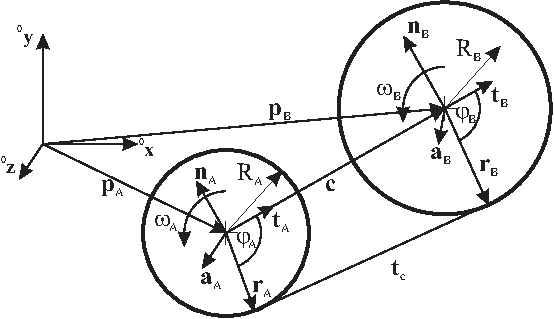
\includegraphics[width=10cm]{figures/CommonTangents3D.pdf}
      \end{center}
      \caption{Geometry of common tangent for two spatial circles defined by radii $R_A$ and $R_B$ as well as by the 
      normalized axis vectors $\av_A$ and $\av_B$. The tangent is undefined, if one of the axis vectors is parallel to the 
      vector $\cv$, which connects the two center points. The positive rotation sense is indicated by means of the 
      angular velocities $\omega_A$ and $\omega_B$.}
        \label{fig:ReevingSystemSprings:tangents}
    \end{figure}
    }
    \onlyRST{
    .. _fig-reevingsystemsprings-tangents:
    .. figure:: docs/theDoc/figures/CommonTangents3D.png
       :width: 500

       Geometry of common tangent for two spatial circles defined by radii $R_A$ and $R_B$ as well as by the normalized axis vectors $\av_A$ and $\av_B$. The tangent is undefined, if one of the axis vectors is parallel to the vector $\cv$, which connects the two center points. The positive rotation sense is indicated by means of the angular velocities $\omega_A$ and $\omega_B$.
    }
    %++++++++++++++++++++++++
    \mysubsubsubsection{Common tangent of two circles in 3D}
    In order to compute the total length of the rope of the reeving system, the tangent of two arbitrary circles in space needs to be computed.
    Considering \fig{fig:ReevingSystemSprings:tangents}, the relations are based on the
    center points of the circles $\pv_A$ and $\pv_B$, the radii $R_A$ and $R_B$ as well as
    the axis vectors $\av_A$ and $\av_B$, the latter vectors also defining the side at which the tangent contacts.
    For the definition of the tangent, the vectors $\rv_A$ and $\rv_B$ need to be computed.
    
    For the special case of $R_A=R_B=0$, it follows that $\rv_A=\pv_A$ and $\rv_B=\pv_B$.
    Otherwise, we first compute the vector between circle centers,
    \be
      \cv = \pv_B - \pv_A, \quad \mathrm{and} \quad \cv_0 = \frac{\cv}{|\cv|} \eqComma
    \ee
    and obtain the tangent vectors
    \be
      \tv_A = \tv_B = \cv_0 \eqComma
    \ee
    as well as the normal vectors
    \be
      \nv_A = \av_A \times \cv_0, \quad \mathrm{and} \quad
      \nv_B = \av_B \times \cv_0 \eqDot
    \ee
    Note that the orientation of the axis vectors $\av_A$ and $\av_B$ defines the orientation of the normals.
    By definition, we assume the following conditions,
    \be
      \nv_A\tp \rv_A < 0, \quad \mathrm{and} \quad 
      \nv_B\tp \rv_B < 0 \eqDot
    \ee
    For two circles with equal radius and axes orientations, the angles result in $\varphi_A=\varphi_B=\pi$.
    In general, the unknown vectors $\rv_A$ and $\rv_B$ are computed by means of Newton's method.
    The unknown tangent vector is given as 
    \be
      \tv_c = \pv_B + \rv_B - \pv_A - \rv_A = \cv + \rv_B - \rv_A \eqDot
    \ee
    We now parameterize the two unknown vectors by means of unknown angles $\varphi_A$ and $\varphi_B$,
    \be
      \rv_A = -R_A \left( \cos(\varphi_A) \tv_A - \sin(\varphi_A) \nv_A \right),
      \quad \mathrm{and} \quad 
      \rv_B = -R_B \left( \cos(\varphi_B) \tv_B - \sin(\varphi_B) \nv_B \right) \eqDot
    \ee
    As vectors $\rv_A$ and $\rv_B$ must be perpendicular to $\tv_c$, it follows that
    \be
      \rv_A\tp (\cv + \rv_B - \rv_A) = 0,
      \quad \mathrm{and} \quad 
      \rv_B\tp (\cv + \rv_B - \rv_A) = 0,
    \ee
    or
    \be \label{eq:ReevingSystemSprings:Newton}
      \rv_A\tp \cv + \rv_A\tp \rv_B - R_A^2 = 0,
      \quad \mathrm{and} \quad 
      \rv_B\tp \cv - \rv_B\tp\rv_A + R_B^2 = 0 \eqDot
    \ee
    The relations \eq{eq:ReevingSystemSprings:Newton} reduce to only one equation, if either $R_A=0$ or $R_B = 0$.
    The equations can be solved by Newton's method by computing the jacobian of $\Jm_{CT}$ of \eq{eq:ReevingSystemSprings:Newton} w.r.t.\ the 
    unknown angles $\varphi_A$ and $\varphi_B$. The iterations are started with
    \be
      \varphi_A = \pi \quad \mathrm{and} \quad \varphi_B = \pi,
    \ee
    and iterate until the error is below a certain tolerance, for details see the implementation in \texttt{Geometry.h}.
    
    \mysubsubsubsection{Connector forces}
    The current rope length results from the configuration of sheaves, including start and end position:
    \be
      L = d_{m_0-m_1} + C_{m_1} + d_{m_1-m_2} + C_{m_2} + \ldots  + d_{m_{nr-2}-m_{nr-1}}
    \ee
    in which $d_{...}$ represents the free spans between two sheaves as computed from the common tangent in the previous section,
    and $C_{...}$ represents the length along the circumference of the according marker if the according radius $r$ is non-zero.
    The quantity $C_{...}$ can be computed easily as soon as the radius vectors to the tangents $\rv_A$ and $\rv_B$
    are known. Within a series of tangents, the previous to the current tangent will always enclose an angle between $0$ and $2\cdot \pi$.
    
    In case that \texttt{hasCoordinateMarkers=True}, the total reference length and its derivative result as
    \be
      L_0 = L_{ref} + f_0 \cdot q_{m_{c0}} + f_1 \cdot q_{m_{c1}}, \quad
      \dot L_0 = f_0 \cdot \dot q_{m_{c0}} + f_1 \cdot \dot q_{m_{c1}}, \quad
    \ee
    while we set $L_0 = L_{ref}$ and $\dot L_0=0$ otherwise.
    The linear force in the reeving system (assumed to be constant all over the rope) is computed as
    \be
      F_{lin} = (L-L_{0}) \frac{EA}{L_0} + (\dot L - \dot L_0)\frac{DA}{L_0}
    \ee
    The rope force is computed from
    \be
      F =   \begin{cases} F_{lin} \quad \mathrm{if} \quad F_{lin} > 0 \\
                          F_{reg} \cdot \mathrm{tanh}(F_{lin}/F_{reg})\quad \mathrm{else} 
            \end{cases}
    \ee
    Which allows small compressive forces $F_{reg}$.
    In case that $F_{reg} < 0$, compressive forces are not regularized (linear spring).
    The case $F_{reg} = 0$ will be used in future only in combination with a data node, 
    which allows switching similar as in friction and contact elements.
    
    Note that in case of $L_0=0$, the term $\frac{1}{L_0}$ is replaced by $1000$.
    However, this case must be avoided by the user by choosing appropriate parameters for the system.

    Additional damping may be added via the parameters $DT$ and $DS$, which have to be treated carefully. The shearing parameter may
    be helpful to damp undesired oscillatory shearing motion, however, it may also damp rigid body motion of the overall mechanism.

    Further details are given in the implementation and examples are provided in the \texttt{Examples} and \texttt{TestModels} folders.
    %%RSTCOMPATIBLE
\vspace{6pt}\par\noindent\rule{\textwidth}{0.4pt}
%
\noindent For examples on ObjectConnectorReevingSystemSprings see Relevant Examples and TestModels with weblink:
\bi
\item \exuUrl{https://github.com/jgerstmayr/EXUDYN/blob/master/main/pythonDev/Examples/craneReevingSystem.py}{\texttt{craneReevingSystem.py}} (Examples/)
\item \exuUrl{https://github.com/jgerstmayr/EXUDYN/blob/master/main/pythonDev/TestModels/reevingSystemSpringsTest.py}{\texttt{reevingSystemSpringsTest.py}} (TestModels/)

\ei

%
\newpage

%+++++++++++++++++++++++++++++++++++

\mysubsubsection{ObjectConnectorRollingDiscPenalty}
\label{sec:item:ObjectConnectorRollingDiscPenalty}
A (flexible) connector representing a rolling rigid disc (marker 1) on a flat surface (marker 0, ground body, not moving) in global $x$-$y$ plane. The connector is based on a penalty formulation and adds friction and slipping. The contraints works for discs as long as the disc axis and the plane normal vector are not parallel. Parameters may need to be adjusted for better convergence (e.g., dryFrictionProportionalZone). The formulation for the arbitrary disc axis is still under development and needs further testing. Note that the rolling body must have the reference point at the center of the disc.
\vspace{12pt}\\

\noindent \mybold{Additional information for ObjectConnectorRollingDiscPenalty}:
\bi
  \item This \texttt{Object} has/provides the following types = \texttt{Connector}
  \item Requested \texttt{Marker} type = \texttt{Position} + \texttt{Orientation}
  \item Requested \texttt{Node} type = \texttt{GenericData}
  \item {\bf Short name} for Python = \texttt{RollingDiscPenalty}
  \item {\bf Short name} for Python visualization object = \texttt{VRollingDiscPenalty}
\ei\vspace{12pt} \noindent 
The item \mybold{ObjectConnectorRollingDiscPenalty} with type = 'ConnectorRollingDiscPenalty' has the following parameters:
\vspace{-0.5cm}\\
\vspace{-0.5cm}\\
%reference manual TABLE
\begin{center}
  \footnotesize
  \begin{longtable}{| p{4.5cm} | p{2.5cm} | p{0.5cm} | p{2.5cm} | p{6cm} |}
    \hline
    \bf Name & \bf type & \bf size & \bf default value & \bf description \\ \hline
    name &     String &      &     '' &     constraints's unique name\\ \hline
    markerNumbers &     ArrayMarkerIndex &     \tabnewline 2 &     [ invalid [-1], invalid [-1] ] &     \tabnewline list of markers used in connector; $m0$ represents a point at the plane surface (normal of surface plane defined by planeNormal); the ground can also be a moving rigid body; $m1$ represents the rolling body, which has its reference point (=local position [0,0,0]) at the disc center point\\ \hline
    nodeNumber &     NodeIndex &      &     invalid (-1) &     \tabnewline node number of a NodeGenericData (size=3) for 3 dataCoordinates, needed for discontinuous iteration (friction and contact)\\ \hline
    discRadius &     PReal &      &     0. &     defines the disc radius\\ \hline
    discAxis &     Vector3D &      &     [1,0,0] &     axis of disc defined in marker $m1$ frame\\ \hline
    planeNormal &     Vector3D &      &     [0,0,1] &     normal to the contact / rolling plane (ground); note that the plane reference point can be arbitrarily chosen by the location of the marker $m0$\\ \hline
    dryFrictionAngle &     Real &      &     0. &     angle [SI:1 (rad)] which defines a rotation of the local tangential coordinates dry friction; this allows to model Mecanum wheels with specified roll angle\\ \hline
    contactStiffness &     UReal &      &     0. &     normal contact stiffness [SI:N/m]\\ \hline
    contactDamping &     UReal &      &     0. &     normal contact damping [SI:N/(m s)]\\ \hline
    dryFriction &     Vector2D &      &     [0,0] &     dry friction coefficients [SI:1] in local marker 1 joint $J1$ coordinates; if $\alpha_t==0$, lateral direction $l=x$ and forward direction $f=y$; assuming a normal force $f_n$, the local friction force can be computed as $\LU{J1}{\vp{f_{t,x}}{f_{t,y}}} = \vp{\mu_x f_n}{\mu_y f_n}$\\ \hline
    dryFrictionProportionalZone &     Real &      &     0. &     limit velocity [m/s] up to which the friction is proportional to velocity (for regularization / avoid numerical oscillations)\\ \hline
    viscousFriction &     Vector2D &      &     [0,0] &     viscous friction coefficients [SI:1/(m/s)] in local marker 1 joint $J1$ coordinates; proportional to slipping velocity, leading to increasing slipping friction force for increasing slipping velocity\\ \hline
    rollingFrictionViscous &     Real &      &     0. &     rolling friction [SI:1], which acts against the velocity of the trail on ground and leads to a force proportional to the contact normal force; currently, only implemented for disc axis parallel to ground!\\ \hline
    useLinearProportionalZone &     Bool &      &     False &     if True, a linear proportional zone is used; the linear zone performs better in implicit time integration as the Jacobian has a constant tangent in the sticking case\\ \hline
    activeConnector &     Bool &      &     True &     flag, which determines, if the connector is active; used to deactivate (temporarily) a connector or constraint\\ \hline
    visualization &     VObjectConnectorRollingDiscPenalty &      &      &     parameters for visualization of item\\ \hline
\end{longtable}
\end{center}

\noindent The item VObjectConnectorRollingDiscPenalty has the following parameters:
%reference manual TABLE
\begin{center}
  \footnotesize
  \begin{longtable}{| p{4.5cm} | p{2.5cm} | p{0.5cm} | p{2.5cm} | p{6cm} |}
    \hline
    \bf Name & \bf type & \bf size & \bf default value & \bf description \\ \hline
    show &     Bool &      &     True &     set true, if item is shown in visualization and false if it is not shown\\ \hline
    discWidth &     float &      &     0.1 &     width of disc for drawing\\ \hline
    color &     Float4 &      &     [-1.,-1.,-1.,-1.] &     \tabnewline RGBA connector color; if R==-1, use default color\\ \hline
\end{longtable}
\end{center}
\par\noindent\rule{\textwidth}{0.4pt}
\mysubsubsubsection{DESCRIPTION of ObjectConnectorRollingDiscPenalty:}
\label{description_ObjectConnectorRollingDiscPenalty}
\paragraph{Information on input parameters:} 
\startTable{input parameter}{symbol}{description see tables above}
\rowTable{markerNumbers}{$[m0,m1]\tp$}{}
\rowTable{nodeNumber}{$n_d$}{}
\rowTable{discAxis}{$\LU{m1}{\wv_{1}}, \;\; |\LU{m1}{\wv_{1}}| = 1$}{}
\rowTable{planeNormal}{$\LU{m0}{\vv_{PN}}, \;\; |\LU{m0}{\vv_{PN}}| = 1$}{}
\rowTable{dryFrictionAngle}{$\alpha_t$}{}
\rowTable{contactStiffness}{$k_c$}{}
\rowTable{contactDamping}{$d_c$}{}
\rowTable{dryFriction}{$[\mu_x,\mu_y]\tp$}{}
\rowTable{dryFrictionProportionalZone}{$v_\mu$}{}
\rowTable{viscousFriction}{$[d_x, d_y]\tp$}{}
\rowTable{rollingFrictionViscous}{$\mu_r$}{}
\finishTable

\mybold{The following output variables are available as OutputVariableType in sensors, Get...Output() and other functions}:
\begin{center}
\footnotesize
\begin{longtable}{| p{5cm} | p{5cm} | p{6cm} |} 
\hline
\bf output variable & \bf symbol & \bf description \\ \hline
Position & $\LU{0}{\pv}_{G}$ & current global position of contact point between rolling disc and ground\\ \hline
Velocity & $\LU{0}{\vv}_{trail}$ & current velocity of the trail (according to motion of the contact point along the trail!) in global coordinates; this is not the velocity of the contact point!\\ \hline
VelocityLocal & $\LU{J1}{\vv}$ & relative slip velocity at contact point in special $J1$ joint coordinates\\ \hline
ForceLocal & $\LU{J1}{\fv} = \LU{0}{[f_{t,x},\, f_{t,y},\, f_{n}]\tp}$ & contact forces acting on disc, in special $J1$ joint coordinates, see section Connector Forces, $f_{t,x}$ being the lateral force (parallel to ground plane), $f_{t,y}$ being the longitudinal force and $f_{n}$ being the contact normal force\\ \hline
RotationMatrix & $\LU{0,J1}{\Am} = [\LU{0}{\wv_{lat}},\, \LU{0}{\wv}_2,\, \LU{0}{\vv_{PN}}]$ & transformation matrix of special joint coordinates $J1$ to global coordinates\\ \hline
\end{longtable}
\end{center}
 \noindent
    \mysubsubsubsection{Definition of quantities}
    \startTable{intermediate variables}{symbol}{description}
    \rowTable{marker m0 position}{$\LU{0}{\pv}_{m0}$}{current global position which is provided by marker m0, any ground reference point; currently unused}
    \rowTable{marker m0 orientation}{$\LU{0,m0}{\Rot}$}{current rotation matrix provided by marker m0; currently unused}
    \rowTable{marker m1 position}{$\LU{0}{\pv}_{m1}$}{center of disc}
    \rowTable{marker m1 orientation}{$\LU{0,m1}{\Rot}$}{current rotation matrix provided by marker m1}
    \rowTable{data coordinates}{$\xv=[x_0,\,x_1,\,x_2]\tp$}{data coordinates for $[x_0,\,x_1]$: hold the sliding velocity in lateral and longitudinal direction of last discontinuous iteration; $x_2$: represents gap of last discontinuous iteration (in contact normal direction)}
    %
    %\rowTable{marker m0 velocity}{$\LU{0}{\vv}_{m0}$}{current global velocity which is provided by marker m0}
    \rowTable{marker m1 velocity}{$\LU{0}{\vv}_{m1}$}{accordingly}
    %\rowTable{marker m0 angular velocity}{$\LU{0}{\tomega}_{m0}$}{current angular velocity vector provided by marker m0}
    \rowTable{marker m1 angular velocity}{$\LU{0}{\tomega}_{m1}$}{current angular velocity vector provided by marker m1}
    %
    \rowTable{ground normal vector}{$\LU{0}{\vv_{PN}} = \LU{0,m0}{\Am} \LU{m0}{\vv_{PN}}$}{normalized normal vector to the ground body (rotates with marker $m0$ if not fixed to ground)}
    \rowTable{ground position B}{$\LU{0}{\pv}_{B}$}{disc center point projected on ground (normal projection)}
    \rowTable{ground position C}{$\LU{0}{\pv}_{C}$}{contact point of disc with ground}
    \rowTable{ground velocity C}{$\LU{0}{\vv}_{C}$}{velocity of disc at ground contact point (must be zero at end of iteration)}
    \rowTable{wheel axis vector}{$\LU{0}{\wv_1} =\LU{0,m1}{\Rot} \LU{m1}{\wv_{1}} $}{normalized disc axis vector in global coordinates}
    \rowTable{longitudinal vector}{$\LU{0}{\wv_2}$}{vector in longitudinal (motion) direction}
    \rowTable{contact point vector}{$\LU{0}{\wv_3}$}{normalized vector from disc center point in direction of contact point C}
    \rowTable{lateral vector}{$\LU{0}{\wv_{lat}} = \LU{0}{\vv_{PN}} \times \LU{0}{\wv}_2$}{vector in lateral direction, parallel to ground plane}
    \rowTable{$D1$ transformation matrix}{$\LU{0,D1}{\Am} = [\LU{0}{\wv_1},\, \LU{0}{\wv_2},\, \LU{0}{\wv_3}]$}{transformation of special disc coordinates $D1$ to global coordinates}
    %
    \rowTable{connector forces}{$\LU{J1}{\fv}=[f_{t,x},\,f_{t,y},\,f_n]\tp$}{joint force vector at contact point in joint 1 coordinates: x=lateral direction, y=longitudinal direction, z=plane normal (contact normal)}
    \finishTable
    
    \mysubsubsubsection{Geometric relations}
    %++++++++++++++++++++++++++++++++++++++++++++++++++++++++++
    \noindent The main geometrical setup is shown in the following figure:
    \ignoreRST{
    \begin{center}
        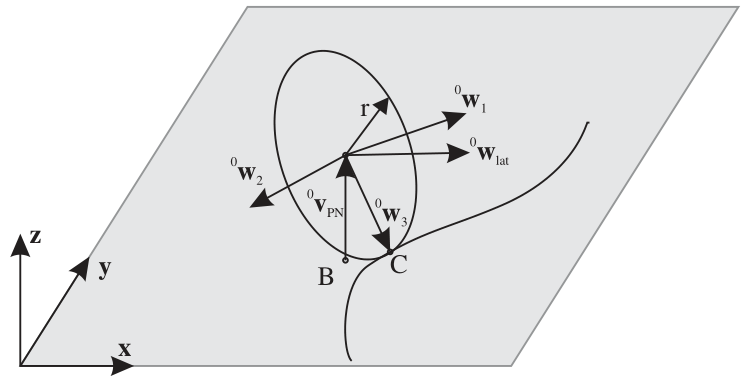
\includegraphics[height=4cm]{figures/ObjectJointRollingDiscSketch.pdf}
    \end{center}
    }
    \onlyRST{
    .. image:: docs/theDoc/figures/ObjectJointRollingDiscSketch.png
       :width: 600

    }
    First, the contact point $\LU{0}{\pv}_{C}$ must be computed.
    With the helper vector,
    \be
      \LU{0}{\xv} = \LU{0}{\wv}_1 \times \LU{0}{\vv_{PN}}
    \ee
    we create a disc coordinate system $D1$ ($\LU{0}{\wv}_1, \; \LU{0}{\wv}_2, \; \LU{0}{\wv}_3$), with the longitudinal direction,
    \be
      \LU{0}{\wv}_2 = \frac{1}{|\LU{0}{\xv}|} \LU{0}{\xv} 
    \ee
    and the vector to the contact point,
    \be
      \LU{0}{\wv}_3 = \LU{0}{\wv}_1 \times \LU{0}{\wv}_2
    \ee
    The vector from marker $m0$ position to the contact point can be computed from
    \be
      \LU{0}{\pv}_{C} = \LU{0}{\pv}_{m1} + r \cdot \LU{0}{\wv}_3 - \LU{0}{\pv}_{m0}
    \ee
    The velocity of the contact point at the disc is computed from,
    \be
      \LU{0}{\vv}_{C} = \LU{0}{\vv}_{m1} + \LU{0}{\tomega}_{m1} \times (r\cdot \LU{0}{\wv}_3)
                        - \left(\LU{0}{\vv}_{m0} + \LU{0}{\tomega}_{m0} \times \LU{0}{\pv}_{C} \right)
    \ee
    A second coordinate system, denoted as $J1$, is defined by vectors ($\LU{0}{\wv}_{lat}, \; \LU{0}{\wv}_2, \;  \LU{0}{\vv}_{PN}$), using
    \be
        \LU{0}{\wv}_{lat} = \LU{0}{\vv_{PN}} \times \LU{0}{\wv}_2
    \ee
    Note that {\bf in the case that} the rolling axis $\LU{0}{\wv}_1$ lies in the rolling plane, we obtain the special case
    $\LU{0}{\wv}_{lat} = \LU{0}{\wv}_1$ and $\LU{0}{\wv}_3 = -\LU{0}{\vv}_{PN}$.
                                                                     
    \mysubsubsubsection{Computation of normal and tangential forces}
    The connector forces at the contact point $C$ are computed as follows. 
    The normal contact force reads
    \be
      f_n = \left(k_c \cdot \LU{0}{\pv}_{C} + d_c \cdot \LU{0}{\vv}_{C} \right)\tp \LU{0}{\vv_{PN}} \eqDot
    \ee
    Note that due to the projection onto $\LU{0}{\vv_{PN}}$, this equation also works for inclined planes
    and reference points, that are not at $[0,0,0]\tp$.
    %
    The inplane velocity in joint coordinates,
    \be
      \LU{J1}{\vv_t} = [\LU{0}{\vv}_{C}\tp \LU{0}{\wv}_{lat}, \; \LU{0}{\vv}_{C}\tp \LU{0}{\wv}_2 ]\tp \eqComma
    \ee
    is used for the computation of tangential forces,
    \be
      \LU{J1}{\fv_t} = [f_{t,x} ,\; f_{t,y}]\tp = \LU{J1}{\tmu} \cdot \left( \phi(|\vv_t|,v_\mu) \cdot f_n \cdot \LU{J1}{\ev_t} \right) \eqComma
    \ee
    with the regularization function, see Geradin and Cardona \cite{GeradinCardona2001} (Sec.\ 7.9.3), if \texttt{useLinearProportionalZone=False},
    \be
      \phi(v, v_\mu) = 
        \left\{ 
            \begin{array}{ccl}
                \displaystyle \left( 2-\frac{v}{v_\mu} \right)\frac{v}{v_\mu} & \mathrm{if} & v \le v_\mu \\
                1 & \mathrm{if} & v > v_\mu \\
            \end{array}
            \right.
    \ee
    and the linear regularization function, if \texttt{useLinearProportionalZone=True},
    \be
      \phi(v, v_\mu) = 
        \left\{ 
            \begin{array}{ccl}
                \displaystyle \frac{v}{v_\mu} & \mathrm{if} & v \le v_\mu \\
                1 & \mathrm{if} & v > v_\mu \\
            \end{array}
            \right.
    \ee
    The direction of tangential slip is given as
    \be
      \LU{J1}{\ev_t} = 
        \left\{ 
            \begin{array}{ccl}
                \displaystyle \frac{\LU{J1}{\vv_t}}{|\vv_t|} &\mathrm{if}& |\vv_t|>0 \\
                %\left[0,\; 0\right]\tp &\mathrm{else}& \\
                \vp{0}{0} &\mathrm{else}& \\
            \end{array}
            \right.
    \ee
    The friction coefficient matrix $\LU{J1}{\tmu}$ is given in joint coordinates and computed from
    \be
      \LU{J1}{\tmu} = \mp{\mu_x + d_x \cdot |\vv_t|}{0}{0}{\mu_y + d_y \cdot |\vv_t|}
    \ee
    where for isotropic behaviour of surface and wheel, it will give a diagonal matrix with the friction coefficient in the diagonal.
    In case that the dry friction angle $\alpha_t$ is not zero, the $\tmu$ changes to
    \be
      \LU{J1}{\tmu} = \mp{\cos(\alpha_t)}{\sin(\alpha_t)}{-\sin(\alpha_t)}{\cos(\alpha_t)} 
      \mp{\mu_x + d_x \cdot |\vv_t|}{0}{0}{\mu_y + d_y \cdot |\vv_t|} 
      \mp{\cos(\alpha_t)}{-\sin(\alpha_t)}{\sin(\alpha_t)}{\cos(\alpha_t)}
    \ee
    %
    \mysubsubsubsection{Connector forces}
    Finally, the connector forces read in joint coordinates
    \be \label{eq:ConnectorRollingDiscPenalty:forces}
      \LU{J1}{\fv} = \vr{f_{t,x}}{f_{t,y}}{f_n}
    \ee
    and in global coordinates, they are computed from
    \be
      \LU{0}{\fv} = f_{t,x}\LU{0}{\wv}_{lat} + f_{t,y} \LU{0}{\wv}_2 + f_n \LU{0}{\vv}_{PN}
    \ee
    Due to the fact that the marker positions are not collocated with the contact point, 
    there are additional torques that need to be considered in the action on the body.
    The torque onto the disc (marker $m1$) is computed as
    \be
      \LU{0}{\ttau_{m1}} = (r\cdot \LU{0}{\wv}_3) \times \LU{0}{\fv}
    \ee
    The torque onto the ground (marker $m0$) is computed as
    \be
      \LU{0}{\ttau_{m0}} = \LU{0}{\pv}_{C} \times \LU{0}{\fv}
    \ee
    Note that if \texttt{activeConnector = False}, we replace \eq{eq:ConnectorRollingDiscPenalty:forces} with
    \be
      \LU{J1}{\fv} = \Null
    \ee
    %%RSTCOMPATIBLE
\vspace{6pt}\par\noindent\rule{\textwidth}{0.4pt}
%
\noindent For examples on ObjectConnectorRollingDiscPenalty see Relevant Examples and TestModels with weblink:
\bi
\item \exuUrl{https://github.com/jgerstmayr/EXUDYN/blob/master/main/pythonDev/Examples/bicycleIftommBenchmark.py}{\texttt{bicycleIftommBenchmark.py}} (Examples/)
\item \exuUrl{https://github.com/jgerstmayr/EXUDYN/blob/master/main/pythonDev/Examples/leggedRobot.py}{\texttt{leggedRobot.py}} (Examples/)
\item \exuUrl{https://github.com/jgerstmayr/EXUDYN/blob/master/main/pythonDev/Examples/mobileMecanumWheelRobotWithLidar.py}{\texttt{mobileMecanumWheelRobotWithLidar.py}} (Examples/)
\item \exuUrl{https://github.com/jgerstmayr/EXUDYN/blob/master/main/pythonDev/Examples/reinforcementLearningRobot.py}{\texttt{reinforcementLearningRobot.py}} (Examples/)
\item \exuUrl{https://github.com/jgerstmayr/EXUDYN/blob/master/main/pythonDev/TestModels/carRollingDiscTest.py}{\texttt{carRollingDiscTest.py}} (TestModels/)
\item \exuUrl{https://github.com/jgerstmayr/EXUDYN/blob/master/main/pythonDev/TestModels/laserScannerTest.py}{\texttt{laserScannerTest.py}} (TestModels/)
\item \exuUrl{https://github.com/jgerstmayr/EXUDYN/blob/master/main/pythonDev/TestModels/mecanumWheelRollingDiscTest.py}{\texttt{mecanumWheelRollingDiscTest.py}} (TestModels/)
\item \exuUrl{https://github.com/jgerstmayr/EXUDYN/blob/master/main/pythonDev/TestModels/rollingCoinPenaltyTest.py}{\texttt{rollingCoinPenaltyTest.py}} (TestModels/)
\item \exuUrl{https://github.com/jgerstmayr/EXUDYN/blob/master/main/pythonDev/TestModels/rollingDiscTangentialForces.py}{\texttt{rollingDiscTangentialForces.py}} (TestModels/)
\item \exuUrl{https://github.com/jgerstmayr/EXUDYN/blob/master/main/pythonDev/TestModels/rotatingTableTest.py}{\texttt{rotatingTableTest.py}} (TestModels/)

\ei

%
\newpage

%+++++++++++++++++++++++++++++++++++

\mysubsubsection{ObjectContactConvexRoll}
\label{sec:item:ObjectContactConvexRoll}
A contact connector representing a convex roll (marker 1) on a flat surface (marker 0, ground body, not moving) in global $x$-$y$ plane. The connector is similar to ObjectConnectorRollingDiscPenalty, but includes a (strictly) convex shape of the roll defined by a polynomial. It is based on a penalty formulation and adds friction and slipping. The formulation is still under development and needs further testing. Note that the rolling body must have the reference point at the center of the disc.
\vspace{12pt}\\

\noindent Author: Manzl Peter
\vspace{12pt}\\

\noindent \mybold{Additional information for ObjectContactConvexRoll}:
\bi
  \item This \texttt{Object} has/provides the following types = \texttt{Connector}
  \item Requested \texttt{Marker} type = \texttt{Position} + \texttt{Orientation}
  \item Requested \texttt{Node} type = \texttt{GenericData}
\ei\vspace{12pt} \noindent 
The item \mybold{ObjectContactConvexRoll} with type = 'ContactConvexRoll' has the following parameters:
\vspace{-0.5cm}\\
\vspace{-0.5cm}\\
%reference manual TABLE
\begin{center}
  \footnotesize
  \begin{longtable}{| p{4.5cm} | p{2.5cm} | p{0.5cm} | p{2.5cm} | p{6cm} |}
    \hline
    \bf Name & \bf type & \bf size & \bf default value & \bf description \\ \hline
    name &     String &      &     '' &     constraints's unique name\\ \hline
    markerNumbers &     ArrayMarkerIndex &     \tabnewline 2 &     [ invalid [-1], invalid [-1] ] &     \tabnewline list of markers used in connector; $m0$ represents the ground, which can undergo translations but not rotations, and $m1$ represents the rolling body, which has its reference point (=local position [0,0,0]) at the roll's center point\\ \hline
    nodeNumber &     NodeIndex &      &     invalid (-1) &     \tabnewline node number of a NodeGenericData (size=3) for 3 dataCoordinates, needed for discontinuous iteration (friction and contact)\\ \hline
    contactStiffness &     Real &      &     0. &     normal contact stiffness [SI:N/m]\\ \hline
    contactDamping &     Real &      &     0. &     normal contact damping [SI:N/(m s)]\\ \hline
    dynamicFriction &     UReal &      &     0. &     dynamic friction coefficient for friction model, see StribeckFunction in exudyn.physics, \refSection{sec:module:physics}\\ \hline
    staticFrictionOffset &     UReal &      &     0. &     static friction offset for friction model (static friction = dynamic friction + static offset), see StribeckFunction in exudyn.physics, \refSection{sec:module:physics}\\ \hline
    viscousFriction &     UReal &      &     0. &     viscous friction coefficient (velocity dependent part) for friction model, see StribeckFunction in exudyn.physics, \refSection{sec:module:physics}\\ \hline
    exponentialDecayStatic &     PReal &      &     1e-3 &     exponential decay of static friction offset (must not be zero!), see StribeckFunction in exudyn.physics (named expVel there!), \refSection{sec:module:physics}\\ \hline
    frictionProportionalZone &     UReal &      &     1e-3 &     limit velocity [m/s] up to which the friction is proportional to velocity (for regularization / avoid numerical oscillations), see StribeckFunction in exudyn.physics (named regVel there!), \refSection{sec:module:physics}\\ \hline
    rollLength &     UReal &      &     0. &     roll length [m], symmetric w.r.t.\ centerpoint\\ \hline
    coefficientsHull &     NumpyVector &      &      [] &     a vector of polynomial coefficients, which provides the polynomial of the CONVEX hull of the roll; $\mathrm{hull}(x) = k_0 x^{n_p-1} + k x^{n_p-2} + \ldots + k_{n_p-2} x  + k_{n_p-1}$\\ \hline
    coefficientsHullDerivative &     NumpyVector &      &     [] &     polynomial coefficients of the polynomial $\mathrm{hull}^\prime(x)$\\ \hline
    coefficientsHullDDerivative &     NumpyVector &      &     [] &     second derivative of the hull polynomial.\\ \hline
    rBoundingSphere &     UReal &      &     0 &     The  radius of the bounding sphere for the contact pre-check, calculated from the polynomial coefficients of the hull\\ \hline
    pContact &     Vector3D &      &     [0,0,0] &     The  current potential contact point. Contact occures if pContact[2] < 0. \\ \hline
    activeConnector &     Bool &      &     True &     flag, which determines, if the connector is active; used to deactivate (temporarily) a connector or constraint\\ \hline
    visualization &     VObjectContactConvexRoll &      &      &     parameters for visualization of item\\ \hline
\end{longtable}
\end{center}

\noindent The item VObjectContactConvexRoll has the following parameters:
%reference manual TABLE
\begin{center}
  \footnotesize
  \begin{longtable}{| p{4.5cm} | p{2.5cm} | p{0.5cm} | p{2.5cm} | p{6cm} |}
    \hline
    \bf Name & \bf type & \bf size & \bf default value & \bf description \\ \hline
    show &     Bool &      &     True &     set true, if item is shown in visualization and false if it is not shown\\ \hline
    color &     Float4 &      &     [-1.,-1.,-1.,-1.] &     \tabnewline RGBA connector color; if R==-1, use default color\\ \hline
\end{longtable}
\end{center}
\par\noindent\rule{\textwidth}{0.4pt}
\mysubsubsubsection{DESCRIPTION of ObjectContactConvexRoll:}
\label{description_ObjectContactConvexRoll}
\paragraph{Information on input parameters:} 
\startTable{input parameter}{symbol}{description see tables above}
\rowTable{markerNumbers}{$[m0,m1]\tp$}{}
\rowTable{nodeNumber}{$n_d$}{}
\rowTable{contactStiffness}{$k_c$}{}
\rowTable{contactDamping}{$d_c$}{}
\rowTable{dynamicFriction}{$\mu_d$}{}
\rowTable{staticFrictionOffset}{$\mu_{s_off}$}{}
\rowTable{viscousFriction}{$\mu_v$}{}
\rowTable{exponentialDecayStatic}{$v_{exp}$}{}
\rowTable{frictionProportionalZone}{$v_{reg}$}{}
\rowTable{rollLength}{$L$}{}
\rowTable{coefficientsHull}{$\kv \in \Rcal^{n_p}$}{}
\rowTable{coefficientsHullDerivative}{$\kv^\prime \in \Rcal^{n_p}$}{}
\finishTable

\mybold{The following output variables are available as OutputVariableType in sensors, Get...Output() and other functions}:
\begin{center}
\footnotesize
\begin{longtable}{| p{5cm} | p{5cm} | p{6cm} |} 
\hline
\bf output variable & \bf symbol & \bf description \\ \hline
Position & $\LU{0}{\pv}_{C}$ & current global position of contact point between roller and ground\\ \hline
Velocity & $\LU{0}{\vv}_{C}$ & current velocity of the trail (contact) point in global coordinates; this is the velocity with which the contact moves over the ground plane\\ \hline
Force & $\LU{0}{\fv}$ & Roll-ground force in ground coordinates\\ \hline
Torque & $\LU{0}{\mv}$ & Roll-ground torque in ground coordinates\\ \hline
\end{longtable}
\end{center}
 \noindent
    \mysubsubsubsection{Definition of quantities}
    \startTable{intermediate variables}{symbol}{description}
    \rowTable{marker m0 position}{$\LU{0}{\pv}_{m0}$}{current global position which is provided by marker m0, any ground reference point; currently unused}
    \rowTable{marker m0 orientation}{$\LU{0,m0}{\Rot}$}{current rotation matrix provided by marker m0; currently unused}
    \rowTable{marker m1 position}{$\LU{0}{\pv}_{m1}$}{center of roll}
    \rowTable{Contact position}{$\LU{0}{\pv}_{C}$}{Position of the Contact point C in the global frame 0}
    \rowTable{Position marker m1 to contact}{$\LU{0}{\pv}_{\mathrm{m1, C}}$}{Position of the contact point C relative to the marker m1 in global frame}
    \rowTable{marker m1 orientation}{$\LU{0,m1}{\Rot}$}{current rotation matrix provided by marker m1}
    \rowTable{data coordinates}{$\xv=[x_0,\,x_1,\,x_2]\tp$}{data coordinates for $[x_0,\,x_1]$: hold the sliding velocity in lateral and longitudinal direction of last discontinuous iteration; $x_2$: represents gap of last discontinuous iteration (in contact normal direction)}
    %
    %\rowTable{marker m0 velocity}{$\LU{0}{\vv}_{m0}$}{current global velocity which is provided by marker m0}
    \rowTable{marker m1 velocity}{$\LU{0}{\vv}_{m1}$}{current global velocity which is provided by marker m1}
    %\rowTable{marker m0 angular velocity}{$\LU{0}{\tomega}_{m0}$}{current angular velocity vector provided by marker m0}
    \rowTable{marker m1 angular velocity}{$\LU{0}{\tomega}_{m1}$}{current angular velocity vector provided by marker m1}
    %
    \rowTable{ground normal vector}{$\LU{0}{\nv}$}{normalized normal vector to the (moving, but not rotating) ground, by default [0,0,1]}
    
    %    \rowTable{ground position B}{$\LU{0}{\pv}_{B}$}{roll center point projected on ground (normal projection)}
    %    \rowTable{ground position C}{$\LU{0}{\pv}_{C}$}{contact point of disc with ground}
    %    \rowTable{ground velocity C}{$\LU{0}{\vv}_{C}$}{velocity of disc at ground contact point (must be zero at end of iteration)}
    %    \rowTable{wheel axis vector}{$\LU{0}{\wv}_1 =\LU{0,m1}{\Rot} \cdot [1,0,0]\tp $}{normalized disc axis vector, currently $[1,0,0]\tp$ in local coordinates}
    %    \rowTable{longitudinal vector}{$\LU{0}{\wv}_2$}{vector in longitudinal (motion) direction}
    %    \rowTable{lateral vector}{$\LU{0}{\wv}_l = \LU{0}{\vv_{PN}} \times \LU{0}{\wv}_2 = [-\wv_{2,y}, \wv_{2,x}, 0]$}{vector in lateral direction, lies in ground plane}
    %    \rowTable{contact point vector}{$\LU{0}{\wv}_3$}{normalized vector from disc center point in direction of contact point C}
    %
    %    \rowTable{connector forces}{$\LU{J1}{\fv}=[f_{t,x},\,f_{t,y},\,f_n]\tp$}{joint force vector at contact point in joint 1 coordinates: x=lateral direction, y=longitudinal direction, z=plane normal (contact normal)}
    \finishTable
    %
    \mysubsubsubsection{Geometric relations}
    %++++++++++++++++++++++++++++++++++++++++++++++++++++++++++
    The geometrical setup is shown in \fig{fig:ObjectContactConvexRoll:sketch}. To calculate the contact point of the convex body of revolution the contact (ground) plane is rotated into the local frame of the body. In this local frame in which the generatrix of the body of revolution is described by the polynomial function
    \be
    \mathrm{r}(^bx) = \sum_{i=0}^n k_i \; x^{n-i} \label{eq:ConnectorConvexRolling:polynomial}
    \ee
    with the coefficients of the hull $a_i$. As a pre-Check for the contact two spheres are put into both ends of the object with the maximum radius and only if one of these is in contact. The contact point $^{\mathrm{b}}\pv_{\mathrm{m1,C}} $ is calculated relative to the bodies marker \texttt{m1} in the bodies local frame and transformed accordingly. 
    The contact point C can for be calculated convex bodies by matching the derivative of the polynomial $r(^bx)$ with the gradient of the contact plane, shown in \fig{fig:ObjectContactConvexRoll:sketch}, explained in detail in \cite{ManzlGerstmayr2021}. 
    At the contact point a normal force $\fv_{\mathrm{N}} = [ 0 \; 0 \; \mathrm{f}_{\mathrm{N}} ]\tp$  with 
    \be
    \mathrm{f}_{\mathrm{N}} = \begin{cases}
    - (k_c \, z_{\mathrm{pen}} + d_c \,  \dot{z}_{\mathrm{pen}})  &\text{$z_{\mathrm{pen}}>0$} \\ % darstellen dämpfung 
    0 &\text{else} \label{eq_FpenContact}
    \end{cases}
    \ee
    acts against the penetration of the ground. The penetration depth $z_{\mathrm{pen}}$ is the z-component of the position vector of the contact point relative to the ground frame ${^0\pv_{\mathrm{C}}}$. 
    \ignoreRST{
    \begin{figure}[tbph]
    \begin{center}
            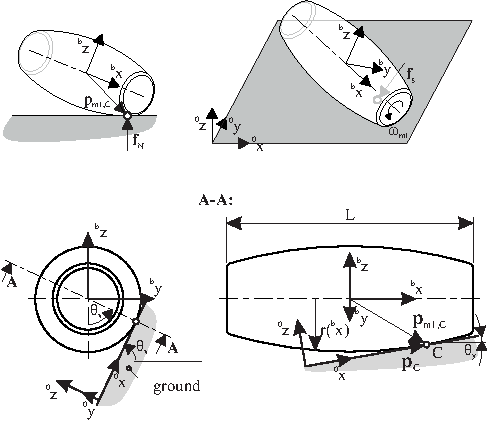
\includegraphics[width=10cm]{figures/ConvexRolling.pdf}
            \caption{Sketch of the roller Dimensions. The rollers radius $r({^bx})$ is described by the polynomial \texttt{coefficientsHull}.}
            \label{fig:ObjectContactConvexRoll:sketch}
    \end{center}
    \end{figure}
    }
    \onlyRST{
    .. _fig-objectcontactconvexroll-sketch:
    .. figure:: docs/theDoc/figures/ConvexRolling.png
       :width: 600

       Sketch of the roller Dimensions. The rollers radius $r({^bx})$ is described by the polynomial \texttt{coefficientsHull}.
    }

    \noindent
    The revolution results in a velocity of 
    \be
    ^{0}\vv_{C} ={^{0}{\tomega_{\mathrm{m1}}}} \times {^{0}{\pv_{\mathrm{m1,\,C}}}}
    \ee
    in the contact point, while the tangential component of the velocity of the body itself with the normal Vector to the contact plane $\nv$ follows to
    \be 
    \LURU{0}{\vv}{\mathrm{m1,\,t}}{} = \LU{0}{\vv_{\mathrm{m1}}} - {^0\nv} \, \left({^0\nv}^T \, \LU{0}{\vv_{\mathrm{m1}}}\right).
    \ee 
    Therefore the slip velocity of the body can be calculated with
    \be
    \LURU{0}{\vv}{\mathrm{s}}{} = \LURU{0}{\vv}{C}{} - {^0\vv_{\mathrm{m1,\,t}}}
    \ee
    and points in the direction 
    \be
    \LURU{0}{\rv}{s}{} = \frac{1}{\left\lVert \LURU{0}{\vv}{\mathrm{s}}{}\right\rVert} {^0{\vv}_{\mathrm{s}}}.
    \ee
    \noindent The slip force is then calculated
    \be
      ^0\fv_{\mathrm{s}} = \mu(\left\lVert\LU{}{^0\vv_{\mathrm{s}}}\right\rVert)  \, \mathrm{f}_{\mathrm{N}} \, {^0\rv_\mathrm{s}}
    \ee
    and uses for the friction coefficient $\mu$ the regularized friction approach from the StribeckFunction, see \refSection{sec:module:physics}. 
    The torque 
    \be
      ^0\ttau = {^0\pv_{\mathrm{m1,\,C}}} \times (^0\fv_{\mathrm{N}} + {^0\fv_{\mathrm{s}}})
    \ee
    acts onto the body, resulting from the slip force acting not in the bodies center. 
    %%RSTCOMPATIBLE
\vspace{6pt}\par\noindent\rule{\textwidth}{0.4pt}
%
\noindent For examples on ObjectContactConvexRoll see Relevant Examples and TestModels with weblink:
\bi
\item \exuUrl{https://github.com/jgerstmayr/EXUDYN/blob/master/main/pythonDev/TestModels/ConvexContactTest.py}{\texttt{ConvexContactTest.py}} (TestModels/)

\ei

%
\newpage

%+++++++++++++++++++++++++++++++++++

\mysubsubsection{ObjectContactCoordinate}
\label{sec:item:ObjectContactCoordinate}
A penalty-based contact condition for one coordinate; the contact gap $g$ is defined as $g=marker.value[1]- marker.value[0] - offset$; the contact force $f_c$ is zero for $gap>0$ and otherwise computed from $f_c = g*contactStiffness + \dot g*contactDamping$; during Newton iterations, the contact force is actived only, if $dataCoordinate[0] <= 0$; dataCoordinate is set equal to gap in nonlinear iterations, but not modified in Newton iterations.
\vspace{12pt}\\

\noindent \mybold{Additional information for ObjectContactCoordinate}:
\bi
  \item This \texttt{Object} has/provides the following types = \texttt{Connector}
  \item Requested \texttt{Marker} type = \texttt{Coordinate}
  \item Requested \texttt{Node} type = \texttt{GenericData}
\ei\vspace{12pt} \noindent 
The item \mybold{ObjectContactCoordinate} with type = 'ContactCoordinate' has the following parameters:
\vspace{-0.5cm}\\
\vspace{-0.5cm}\\
%reference manual TABLE
\begin{center}
  \footnotesize
  \begin{longtable}{| p{4.5cm} | p{2.5cm} | p{0.5cm} | p{2.5cm} | p{6cm} |}
    \hline
    \bf Name & \bf type & \bf size & \bf default value & \bf description \\ \hline
    name &     String &      &     '' &     connector's unique name\\ \hline
    markerNumbers &     ArrayMarkerIndex &     \tabnewline  &     [ invalid [-1], invalid [-1] ] &     \tabnewline markers define contact gap\\ \hline
    nodeNumber &     NodeIndex &      &     invalid (-1) &     \tabnewline node number of a NodeGenericData for 1 dataCoordinate (used for active set strategy ==> holds the gap of the last discontinuous iteration)\\ \hline
    contactStiffness &     UReal &      &     0. &     contact (penalty) stiffness [SI:N/m]; acts only upon penetration\\ \hline
    contactDamping &     UReal &      &     0. &     contact damping [SI:N/(m s)]; acts only upon penetration\\ \hline
    offset &     Real &      &     0. &     offset [SI:m] of contact\\ \hline
    activeConnector &     Bool &      &     True &     flag, which determines, if the connector is active; used to deactivate (temporarily) a connector or constraint\\ \hline
    visualization &     VObjectContactCoordinate &      &      &     parameters for visualization of item\\ \hline
\end{longtable}
\end{center}

\noindent The item VObjectContactCoordinate has the following parameters:
%reference manual TABLE
\begin{center}
  \footnotesize
  \begin{longtable}{| p{4.5cm} | p{2.5cm} | p{0.5cm} | p{2.5cm} | p{6cm} |}
    \hline
    \bf Name & \bf type & \bf size & \bf default value & \bf description \\ \hline
    show &     Bool &      &     True &     set true, if item is shown in visualization and false if it is not shown\\ \hline
    drawSize &     float &      &     -1. &     drawing size = diameter of spring; size == -1.f means that default connector size is used\\ \hline
    color &     Float4 &      &     [-1.,-1.,-1.,-1.] &     \tabnewline RGBA connector color; if R==-1, use default color\\ \hline
\end{longtable}
\end{center}
\par\noindent\rule{\textwidth}{0.4pt}
\mysubsubsubsection{DESCRIPTION of ObjectContactCoordinate:}
\label{description_ObjectContactCoordinate}
\vspace{6pt}\par\noindent\rule{\textwidth}{0.4pt}
%
\noindent For examples on ObjectContactCoordinate see Relevant Examples and TestModels with weblink:
\bi
\item \exuUrl{https://github.com/jgerstmayr/EXUDYN/blob/master/main/pythonDev/Examples/ANCFcontactCircle.py}{\texttt{ANCFcontactCircle.py}} (Examples/)
\item \exuUrl{https://github.com/jgerstmayr/EXUDYN/blob/master/main/pythonDev/Examples/ANCFcontactCircle2.py}{\texttt{ANCFcontactCircle2.py}} (Examples/)
\item \exuUrl{https://github.com/jgerstmayr/EXUDYN/blob/master/main/pythonDev/TestModels/ANCFcontactCircleTest.py}{\texttt{ANCFcontactCircleTest.py}} (TestModels/)
\item \exuUrl{https://github.com/jgerstmayr/EXUDYN/blob/master/main/pythonDev/TestModels/contactCoordinateTest.py}{\texttt{contactCoordinateTest.py}} (TestModels/)

\ei

%
\newpage

%+++++++++++++++++++++++++++++++++++

\mysubsubsection{ObjectContactCircleCable2D}
\label{sec:item:ObjectContactCircleCable2D}
A very specialized penalty-based contact condition between a 2D circle (=marker0, any Position-marker) on a body and an ANCFCable2DShape (=marker1, Marker: BodyCable2DShape), in xy-plane; a node NodeGenericData is required with the number of cordinates according to the number of contact segments; the contact gap $g$ is integrated (piecewise linear) along the cable and circle; the contact force $f_c$ is zero for $gap>0$ and otherwise computed from $f_c = g*contactStiffness + \dot g*contactDamping$; during Newton iterations, the contact force is actived only, if $dataCoordinate[0] <= 0$; dataCoordinate is set equal to gap in nonlinear iterations, but not modified in Newton iterations.
\vspace{12pt}\\

\noindent \mybold{Additional information for ObjectContactCircleCable2D}:
\bi
  \item This \texttt{Object} has/provides the following types = \texttt{Connector}
  \item Requested \texttt{Marker} type = \texttt{\_None}
  \item Requested \texttt{Node} type = \texttt{GenericData}
\ei\vspace{12pt} \noindent 
The item \mybold{ObjectContactCircleCable2D} with type = 'ContactCircleCable2D' has the following parameters:
\vspace{-0.5cm}\\
\vspace{-0.5cm}\\
%reference manual TABLE
\begin{center}
  \footnotesize
  \begin{longtable}{| p{4.5cm} | p{2.5cm} | p{0.5cm} | p{2.5cm} | p{6cm} |}
    \hline
    \bf Name & \bf type & \bf size & \bf default value & \bf description \\ \hline
    name &     String &      &     '' &     connector's unique name\\ \hline
    markerNumbers &     ArrayMarkerIndex &     \tabnewline  &     [ invalid [-1], invalid [-1] ] &     \tabnewline markers define contact gap\\ \hline
    nodeNumber &     NodeIndex &      &     invalid (-1) &     \tabnewline node number of a NodeGenericData for nSegments dataCoordinates (used for active set strategy ==> hold the gap of the last discontinuous iteration and the friction state)\\ \hline
    numberOfContactSegments &     Index &      &     3 &     number of linear contact segments to determine contact; each segment is a line and is associated to a data (history) variable; must be same as in according marker\\ \hline
    contactStiffness &     UReal &      &     0. &     contact (penalty) stiffness [SI:N/m/(contact segment)]; the stiffness is per contact segment; specific contact forces (per length) $f_N$ act in contact normal direction only upon penetration\\ \hline
    contactDamping &     UReal &      &     0. &     contact damping [SI:N/(m s)/(contact segment)]; the damping is per contact segment; acts in contact normal direction only upon penetration\\ \hline
    circleRadius &     UReal &      &     0. &     radius [SI:m] of contact circle\\ \hline
    offset &     Real &      &     0. &     offset [SI:m] of contact, e.g. to include thickness of cable element\\ \hline
    activeConnector &     Bool &      &     True &     flag, which determines, if the connector is active; used to deactivate (temporarily) a connector or constraint\\ \hline
    visualization &     VObjectContactCircleCable2D &      &      &     parameters for visualization of item\\ \hline
\end{longtable}
\end{center}

\noindent The item VObjectContactCircleCable2D has the following parameters:
%reference manual TABLE
\begin{center}
  \footnotesize
  \begin{longtable}{| p{4.5cm} | p{2.5cm} | p{0.5cm} | p{2.5cm} | p{6cm} |}
    \hline
    \bf Name & \bf type & \bf size & \bf default value & \bf description \\ \hline
    show &     Bool &      &     True &     set true, if item is shown in visualization and false if it is not shown\\ \hline
    showContactCircle &     Bool &      &     True &     if True and show=True, the underlying contact circle is shown; uses circleTiling*4 for tiling (from VisualizationSettings.general)\\ \hline
    drawSize &     float &      &     -1. &     drawing size = diameter of spring; size == -1.f means that default connector size is used\\ \hline
    color &     Float4 &      &     [-1.,-1.,-1.,-1.] &     \tabnewline RGBA connector color; if R==-1, use default color\\ \hline
\end{longtable}
\end{center}
\par\noindent\rule{\textwidth}{0.4pt}
\mysubsubsubsection{DESCRIPTION of ObjectContactCircleCable2D:}
\label{description_ObjectContactCircleCable2D}
 \noindent
    \mysubsubsubsection{Connector equations}
    Geometry and equations are very similar to \texttt{ObjectContactFrictionCircleCable2D}, while friction is not used and no torque
    is transferred to the circle object.
%
\vspace{6pt}\par\noindent\rule{\textwidth}{0.4pt}
%
\noindent For examples on ObjectContactCircleCable2D see Relevant Examples and TestModels with weblink:
\bi
\item \exuUrl{https://github.com/jgerstmayr/EXUDYN/blob/master/main/pythonDev/Examples/ANCFcontactCircle.py}{\texttt{ANCFcontactCircle.py}} (Examples/)
\item \exuUrl{https://github.com/jgerstmayr/EXUDYN/blob/master/main/pythonDev/Examples/ANCFcontactCircle2.py}{\texttt{ANCFcontactCircle2.py}} (Examples/)
\item \exuUrl{https://github.com/jgerstmayr/EXUDYN/blob/master/main/pythonDev/Examples/ANCFmovingRigidbody.py}{\texttt{ANCFmovingRigidbody.py}} (Examples/)
\item \exuUrl{https://github.com/jgerstmayr/EXUDYN/blob/master/main/pythonDev/Examples/ANCFslidingJoint2D.py}{\texttt{ANCFslidingJoint2D.py}} (Examples/)
\item \exuUrl{https://github.com/jgerstmayr/EXUDYN/blob/master/main/pythonDev/TestModels/ANCFcontactCircleTest.py}{\texttt{ANCFcontactCircleTest.py}} (TestModels/)
\item \exuUrl{https://github.com/jgerstmayr/EXUDYN/blob/master/main/pythonDev/TestModels/ANCFmovingRigidBodyTest.py}{\texttt{ANCFmovingRigidBodyTest.py}} (TestModels/)
\item \exuUrl{https://github.com/jgerstmayr/EXUDYN/blob/master/main/pythonDev/TestModels/ANCFslidingAndALEjointTest.py}{\texttt{ANCFslidingAndALEjointTest.py}} (TestModels/)

\ei

%
\newpage

%+++++++++++++++++++++++++++++++++++

\mysubsubsection{ObjectContactFrictionCircleCable2D}
\label{sec:item:ObjectContactFrictionCircleCable2D}
A very specialized penalty-based contact/friction condition between a 2D circle in the local x/y plane (=marker0, a RigidBody Marker, from node or object) on a body and an ANCFCable2DShape (=marker1, Marker: BodyCable2DShape), in xy-plane; a node NodeGenericData is required with 3$\times$(number of contact segments) -- containing per segment: [contact gap, stick/slip (stick=0, slip=+-1, undefined=-2), last friction position]. The connector works with Cable2D and ALECable2D, HOWEVER, due to conceptual differences the (tangential) frictionStiffness cannot be used with ALECable2D; if using, it gives wrong tangential stresses, even though it may work in general.
\vspace{12pt}\\

\noindent \mybold{Additional information for ObjectContactFrictionCircleCable2D}:
\bi
  \item This \texttt{Object} has/provides the following types = \texttt{Connector}
  \item Requested \texttt{Marker} type = \texttt{\_None}
  \item Requested \texttt{Node} type = \texttt{GenericData}
\ei\vspace{12pt} \noindent 
The item \mybold{ObjectContactFrictionCircleCable2D} with type = 'ContactFrictionCircleCable2D' has the following parameters:
\vspace{-0.5cm}\\
\vspace{-0.5cm}\\
%reference manual TABLE
\begin{center}
  \footnotesize
  \begin{longtable}{| p{4.5cm} | p{2.5cm} | p{0.5cm} | p{2.5cm} | p{6cm} |}
    \hline
    \bf Name & \bf type & \bf size & \bf default value & \bf description \\ \hline
    name &     String &      &     '' &     connector's unique name\\ \hline
    markerNumbers &     ArrayMarkerIndex &     \tabnewline  &     [ invalid [-1], invalid [-1] ] &     \tabnewline a marker $m0$ with position and orientation and a marker $m1$ of type BodyCable2DShape; together defining the contact geometry\\ \hline
    nodeNumber &     NodeIndex &      &     invalid (-1) &     \tabnewline node number of a NodeGenericData with 3 $\times n_{cs}$  dataCoordinates (used for active set strategy $\ra$ hold the gap of the last discontinuous iteration, friction state (+-1=slip, 0=stick, -2=undefined) and the last sticking position; initialize coordinates with list [0.1]*$n_{cs}$+[-2]*$n_{cs}$+[0.]*$n_{cs}$, meaning that there is no initial contact with undefined slip/stick\\ \hline
    numberOfContactSegments &     PInt &      &     3 &     number of linear contact segments to determine contact; each segment is a line and is associated to a data (history) variable; must be same as in according marker\\ \hline
    contactStiffness &     UReal &      &     0. &     contact (penalty) stiffness [SI:N/m/(contact segment)]; the stiffness is per contact segment; specific contact forces (per length) $f_n$ act in contact normal direction only upon penetration\\ \hline
    contactDamping &     UReal &      &     0. &     contact damping [SI:N/(m s)/(contact segment)]; the damping is per contact segment; acts in contact normal direction only upon penetration\\ \hline
    frictionVelocityPenalty &     UReal &      &     0. &     tangential velocity dependent penalty coefficient for friction [SI:N/(m s)/(contact segment)]; the coefficient causes tangential (contact) forces against relative tangential velocities in the contact area\\ \hline
    frictionStiffness &     UReal &      &     0. &     tangential displacement dependent penalty/stiffness coefficient for friction [SI:N/m/(contact segment)]; the coefficient causes tangential (contact) forces against relative tangential displacements in the contact area\\ \hline
    frictionCoefficient &     UReal &      &     0. &     friction coefficient [SI: 1]; tangential specific friction forces (per length) $f_t$ must fulfill the condition $f_t \le \mu f_n$\\ \hline
    circleRadius &     UReal &      &     0. &     radius [SI:m] of contact circle\\ \hline
    useSegmentNormals &     Bool &      &     True &      True: use normal and tangent according to linear segment; this is appropriate for very long (compared to circle) segments; False: use normals at segment points according to vector to circle center; this is more consistent for short segments, as forces are only applied in beam tangent and normal direction\\ \hline
    activeConnector &     Bool &      &     True &     flag, which determines, if the connector is active; used to deactivate (temporarily) a connector or constraint\\ \hline
    visualization &     VObjectContactFrictionCircleCable2D &      &      &     parameters for visualization of item\\ \hline
\end{longtable}
\end{center}

\noindent The item VObjectContactFrictionCircleCable2D has the following parameters:
%reference manual TABLE
\begin{center}
  \footnotesize
  \begin{longtable}{| p{4.5cm} | p{2.5cm} | p{0.5cm} | p{2.5cm} | p{6cm} |}
    \hline
    \bf Name & \bf type & \bf size & \bf default value & \bf description \\ \hline
    show &     Bool &      &     True &     set True, if item is shown in visualization and false if it is not shown; note that only normal contact forces can be  drawn, which are approximated by $k_c \cdot g$ (neglecting damping term)\\ \hline
    showContactCircle &     Bool &      &     True &     if True and show=True, the underlying contact circle is shown; uses circleTiling*4 for tiling (from VisualizationSettings.general)\\ \hline
    drawSize &     float &      &     -1. &     drawing size = diameter of spring; size == -1.f means that default connector size is used\\ \hline
    color &     Float4 &      &     [-1.,-1.,-1.,-1.] &     \tabnewline RGBA connector color; if R==-1, use default color\\ \hline
\end{longtable}
\end{center}
\par\noindent\rule{\textwidth}{0.4pt}
\mysubsubsubsection{DESCRIPTION of ObjectContactFrictionCircleCable2D:}
\label{description_ObjectContactFrictionCircleCable2D}
\paragraph{Information on input parameters:} 
\startTable{input parameter}{symbol}{description see tables above}
\rowTable{markerNumbers}{$[m0,m1]\tp$}{}
\rowTable{nodeNumber}{$n_g$}{}
\rowTable{numberOfContactSegments}{$n_{cs}$}{}
\rowTable{contactStiffness}{$k_c$}{}
\rowTable{contactDamping}{$d_c$}{}
\rowTable{frictionVelocityPenalty}{$\mu_v$}{}
\rowTable{frictionStiffness}{$\mu_k$}{}
\rowTable{frictionCoefficient}{$\mu$}{}
\rowTable{circleRadius}{$r$}{}
\finishTable

\mybold{The following output variables are available as OutputVariableType in sensors, Get...Output() and other functions}:
\begin{center}
\footnotesize
\begin{longtable}{| p{5cm} | p{5cm} | p{6cm} |} 
\hline
\bf output variable & \bf symbol & \bf description \\ \hline
Coordinates & $[u_{t,0},\, g_0,\, u_{t,1},\, g_1,\, \ldots,\, u_{t,n_{cs}},\, g_{n_{cs}}]\tp$ & local (relative) displacement in tangential ($\tv$) and normal ($\nv$) direction per segment ($n_{cs}$); values are only provided in case of contact, otherwise zero; tangential displacement is only non-zero in case of sticking!\\ \hline
Coordinates\_t & $[v_{t,0},\, v_{n,0},\, v_{t,1},\, v_{n,1},\, \ldots,\, v_{t,n_{cs}},\, v_{n,n_{cs}}]\tp$ & local (relative) velocity in tangential ($\tv$) and normal ($\nv$) direction per segment ($n_{cs}$); values are only provided in case of contact, otherwise zero\\ \hline
ForceLocal & $[f_{t,0},\, f_{n,0},\, f_{t,1},\, f_{n,1},\, \ldots,\, f_{t,n_{cs}},\, f_{n,n_{cs}}]\tp$ & local contact forces in tangential ($\tv$) and normal ($\nv$) direction per segment ($n_{cs}$)\\ \hline
\end{longtable}
\end{center}
 \noindent
    \mysubsubsubsection{Definition of quantities}
    \startTable{intermediate variables}{symbol}{description}
    \rowTable{marker m0 position}{$\LU{0}{\pv}_{m0}$}{represents current global position of the circle's centerpoint}
    \rowTable{marker m0 velocity}{$\LU{0}{\vv}_{m0}$}{current global velocity which is provided by marker m0}
    \rowTable{marker m1}{}{represents the 2D ANCF cable}
    \rowTable{data node}{$\xv=[x_{i},\; \ldots,\; x_{3 n_{cs} -1}]\tp$}{coordinates of node with node number $n_{GD}$}
    \rowTable{data coordinates for segment $i$}{$[x_i,\, x_{n_{cs}+ i},\, x_{2\cdot n_{cs}+ i}]\tp = [x_{gap},\, x_{isSlipStick},\, x_{lastStick}]\tp$, with $i \in [0,n_{cs}-1]$}{
              The data coordinates include the gap $x_{gap}$, the stick-slip state $x_{isSlipStick}$ and the previous sticking position $x_{lastStick}$ as computed in the PostNewtonStep, see description below. }
    \rowTable{shortest distance to segment $s_i$}{$\dv_{g,i}$}{shortest distance of center of circle to contact segment, considering the endpoint of the segment}
    %\rowTable{marker m1 velocity}{$\LU{0}{\vv}_{m1}$}{}
    \finishTable
    %++++++++++++++++++++++++
    \ignoreRST{
    \begin{figure}[tbph]
      \begin{center}
      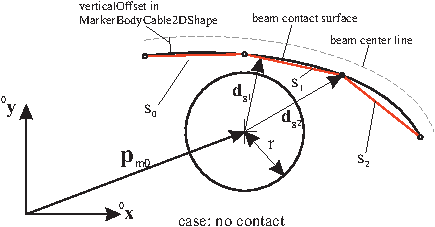
\includegraphics[width=12cm]{figures/ContactFrictionCircleCable2D.pdf}
      \end{center}
      \caption{Sketch of cable, contact segments and circle; showing case without contact, $|\dv_{g1}| > r$, 
               while contact occurs with $|\dv_{g1}| \le r$; the shortest distance vector $\dv_{g1}$
               is related to segment $s_1$ (which is perpendicular to the the segment line) and 
               $\dv_{g2}$ is the shortest distance to the end point of segment $s_2$, not being
               perpendicular.}
        \label{fig:ObjectContactFrictionCircleCable2D:sketch}
    \end{figure}
    }
    \onlyRST{
    .. _fig-objectcontactfrictioncirclecable2d-sketch:
    .. figure:: docs/theDoc/figures/ContactFrictionCircleCable2D.png
       :width: 600

       Sketch of cable, contact segments and circle; showing case without contact, $|\mathbf{d}_{g1}| > r$, while contact occurs with $|\mathbf{d}_{g1}| \le r$; the shortest distance vector $\mathbf{d}_{g1}$ is related to segment $s_1$ (which is perpendicular to the the segment line) and $\mathbf{d}_{g2}$ is the shortest distance to the end point of segment $s_2$, not being perpendicular
    }
    %+++++++++++++++++++++++++++++++++++++++++++++++
    \mysubsubsubsection{Connector forces: contact geometry}
    %
    The connector represents a force element between a 'circle' (or cylinder) represented by a marker $m0$, which has position and orientation,
    and an \texttt{ANCFCable2D} beam element (denoted as 'cable') represented by a \texttt{MarkerBodyCable2DShape} $m1$.
    The cable with reference length $L$ is discretized by splitting into $n_{cs}$ straight segments $s_i$, located between points $p_i$ and $p_{i+1}$.
    Note that these points can be placed with an offset from the cable centerline, see \texttt{verticalOffset} defined in \texttt{MarkerBodyCable2DShape}.
    In order to compute the gap function for a line segment, the shortest distance of one line segment with
    points $\pv_i$, $\pv_{i+1}$ to the circle's centerpoint given by the marker $\pv_{m0}$ is computed. 
    All computations here are performed in the global coordinates system (0), 
    including edge points of every segment.

    With the intermediate quantities (all of them related to segment $s_i$)\footnote{we omit $s_i$ in some terms for brevity!},
    \be
      \vv_s = \pv_{i+1} - \pv_i, \quad
      \vv_p = \pv_{m0} - \pv_i, \quad
      n = \vv_s\tp \vv_p, \quad
      d = \vv_s\tp \vv_s
    \ee
    and assuming that $d \neq 0$ (otherwise the two segment points would be identical and
    the shortest distance would be $d_g = |\vv_p|$),
    we find the relative position $\rho$ of the shortest (projected) point on the 
    segment, which runs from 0 to 1 if lying on the segment, as
    \be
      \rho = \frac{n}{d}
    \ee
    We distinguish 3 cases (see also \fig{fig:ObjectContactFrictionCircleCable2D:sketch} for cases 1 and 2):
        \bn
        \item If $\rho \le 0$, the shortest distance would be the distance to point $\pv_p=\pv_i$,
        reading 
        \be
          d_g = |\pv_{m0} - \pv_i| \quad (\rho \le 0)
        \ee
        \item If $\rho \ge 1$, the shortest distance would be the distance to point $\pv_p=\pv_{i+1}$,
        reading 
        \be
          d_g = |\pv_{m0} - \pv_{i+1}| \quad (\rho \ge 1)
        \ee
        \item Finally, if $0 < \rho < 1$, then the shortest distance has a projected point somewhere
        on the segment with the point (projected on the segment)
        \be
          \pv_p = \pv_i + \rho \cdot \vv_s
        \ee
        and the distance
        \be
          d_g = |\dv_g| = \sqrt{\vv_p\tp \vv_p - (n^2)/d}
        \ee
    \en
    Here, the shortest distance vector for every segment results from the projected point $\pv_p$ 
    of the above mentioned cases, see also \fig{fig:ObjectContactFrictionCircleCable2D:sketch},
    with the relation
    \be
      \dv_g = \dv_{g,s_i}= \pv_{m0} - \pv_p \eqDot
    \ee
    The contact gap for a specific point for segment $s_i$ is in general defined as
    \be \label{ObjectContactFrictionCircleCable2D:gap}
      g = g_{s_i} = d_g - r \eqDot
    \ee
    using $d_g = |\dv_g|$.
    
    %++++++++++++++++++++++++++++++++++++++++++++++
    \mysubsubsubsection{Contact frame and relative motion}
    %FRAME
    Irrespective of the choice of \texttt{useSegmentNormals}, the contact normal vector $\nv_{s_i}$ and tangential vector $\tv_{s_i}$ are defined per segment as
    \be
      \nv_{s_i} = \nv = [n_0, n_1]\tp = \frac{1}{|\dv_{g,s_i}|} \dv_{g,s_i}, \quad \tv_{s_i} = \tv = [-n_1, n_0]\tp
    \ee
    The vectors $\tv_{s_i}$ and $\nv_{s_i}$ define the local (contact) frame for further computations.
    
    The velocity at the closest point of the segment $s_i$ is interpolated using $\rho$ and computed as
    \be
      \dot \pv_p = (1-\rho) \cdot \vv_i + \rho \cdot \vv_{i+1}
    \ee
    Alternatively, $\dot \pv_p$ could be computed from the cable element by evaluating the velocity at the contact points, but we feel that
    this choice is more consistent with the computations at position level.
    
    The gap velocity $v_n$ ($\neq \dot g$) thus reads
    \be
      v_n = \left( \dot \pv_p - \dot \pv_{m0} \right) \nv
    \ee
    In a similar, the tangential velocity reads
    \be \label{ObjectContactFrictionCircleCable2D:vTangent}
      v_t = \left( \dot \pv_p - \dot \pv_{m0} \right) \tv
    \ee
    In case of \texttt{frictionStiffness != 0}, we continuously track the sticking position at which the cable element (or segment) and the circle 
    previously sticked together, similar as proposed by Lugr{\'i}s et al.~\cite{LugrisEscalonaDC2011}. 
    The difference here to the latter reference, is that we explicitly exclude switching from Newton's method and that Lugr{\'i}s et al.~used
    contact points, while we use linear segments.
    For a simple 1D example using this position based approach for friction, see \texttt{Examples/lugreFrictionText.py}, 
    which compares the traditional LuGre friction model \cite{CanudasDeWitEtAl1993} with the position based model with tangential stiffness. 
    %++++++++++++++++++++++++
    \ignoreRST{
    \begin{figure}[tbph]
      \begin{center}
      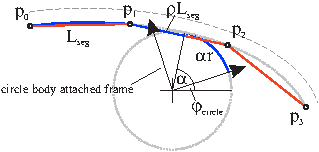
\includegraphics[width=8cm]{figures/ContactFrictionCircleCable2DstickingPos.pdf}
      \end{center}
      \caption{Calculation of last sticking position; blue parts mark the sticking position calculated as $x^*_{curStick}$.}
        \label{fig:ObjectContactFrictionCircleCable2D:stickingPos}
    \end{figure}
    }
    \onlyRST{
    .. _fig-objectcontactfrictioncirclecable2d-stickingpos:
    .. figure:: docs/theDoc/figures/ContactFrictionCircleCable2DstickingPos.png
       :width: 600

       Calculation of last sticking position; blue parts mark the sticking position calculated as $x^*_{curStick}$.
    }
    %++++++++++++++++++++++++
    
    Because there is the chance to wind/unwind relative to the (last) sticking position without slipping,
    the following strategy is used.
    In case of sliding (which could be the last time sliding before sticking), 
    we compute the {\bf current sticking position}, see \fig{fig:ObjectContactFrictionCircleCable2D:stickingPos}, as the sum of the relative position at the segment $s$
    \be
      x_{s,curStick} = \rho \cdot L_{seg}
    \ee
    in which $\rho \in [0,1]$ denotes the relative position of contact at the segment with reference length $L_{seg}=\frac{L}{n_{cs}}$.
    The relative position at the circle $c$ is
    \be
      x_{c,curStick} = \alpha \cdot r
    \ee
    We immediately see, that under pure rolling\footnote{neglecting the effects of small penetration, usually much smaller than shown for visibility in \fig{fig:ObjectContactFrictionCircleCable2D:stickingPos}.},
    \be
      x_{s,curStick} + x_{c,curStick}  = \mathrm{const}.
    \ee
    Note that the \texttt{verticalOffset} from the cable center line, as defined in the related \texttt{MarkerBodyCable2DShape},
    influences the behavior significantly, which is why we recommend to use \texttt{verticalOffset=0} whenever this is an 
    appropriate assumption.
    %include in paper:
    %Even thought that we are convinced that this has some effect, especially for beams with larger height, a reduction of segment length reduces
    %this effects as less (un-)winding occurs, a more consistent computation of this effect would require an
    %integration of relative motion as stretch influences the local changes of the relative sticking position.
    Thus, the current sticking position $x_{curStick}$ is computed per segment as
    \be  \label{ObjectContactFrictionCircleCable2D:lastCurStick}
      x^*_{curStick} = x_{s,curStick} + x_{c,curStick}, \quad
    \ee
    %
    Due to the possibility of switching of $\alpha+\phi$ between $-\pi$ and $\pi$, the result is normalized to
    \be \label{ObjectContactFrictionCircleCable2D:curStick}
      x_{curStick} = x^*_{curStick} - \mathrm{floor}\left(\frac{x^*_{curStick} }{2 \pi \cdot r} + \frac{1}{2}\right) \cdot 2 \pi \cdot r, \quad
    \ee
    which gives $\bar x_{curStick} \in [-\pi \cdot r,\pi \cdot r]$, which is stored in the 3rd data variable (per segment).
    The function floor() is a standardized version of rounding, available in C and Python programming languages.
    In the \texttt{PostNewtonStep}, the last sticking position is computed, $x_{lastStick} = x_{curStick}$, and it is also available in the \texttt{startOfStep} state.

    %++++++++++++++++++++++++++++++++++++++++++++++
    \mysubsubsubsection{Contact forces: definition}
    %FORCES
    The contact force $f_n$ is zero for $g > 0$ and otherwise computed from 
    \be \label{ObjectContactFrictionCircleCable2D:contactForce}
      f_n = k_c \cdot g + d_c \cdot v_n
    \ee
    NOTE that currently, there is only a linear spring-damper model available, assuming that the impact dynamics 
    is not dominating (such as in belt drives or reeving systems).

    Friction forces are primarily based on relative (tangential) velocity at each segment.
    The 'linear' friction force, based on the velocity penalty parameter $\mu_v$ reads
    \be
      f_t^{(lin)} = \mu_v \cdot v_t \eqComma
    \ee    
    %++++++++++++++++++++++++++++++++++++++++++++++
    \mysubsubsubsection{PostNewtonStep}
    In general, see the solver flow chart for the \texttt{DiscontinuousIteration}, see \fig{fig_solver_discontinuous_iteration}, should be considered when reading this description. Every step is started with values \texttt{startOfStep}, while current values are iterated and updated in the Newton or \texttt{DiscontinuousIteration}.
    
    The \texttt{PostNewtonStep} computes 3 values per segment, which are used for computation of contact forces, irrespectively of the 
    current geometryof the contact. 
    The \texttt{PostNewtonStep} is called after every full Newton method and evaluates the current state w.r.t. the assumed data variables.
    If the assumptions do not fit, new data variables are computed.
    This is necessary in order to avoid discontinuities in the equations, while otherwise the Newton iterations would not 
    (or only slowly) converge.

    The data variables per segment are
    \be
      [x_{gap},\, x_{isSlipStick},\, x_{lastStick}]
    \ee
    Here, $x_{gap}$ contains the gap of the segment ($\le 0$ means contact), $x_{lastStick}$ is described in 
    \eq{ObjectContactFrictionCircleCable2D:curStick}, and 
    $x_{isSlipStick}$ defines the stick or slip case,
    \bi
      \item $x_{isSlipStick} = -2$: undefined, used for initialization
      \item $x_{isSlipStick} = 0$: sticking
      \item $x_{isSlipStick} = \pm 1$: slipping, sign defines slipping direction
    \ei
    
    The basic algorithm in the \texttt{PostNewtonStep}, with all operations given for any segment $s_i$, can be summarized as follows:
    \bi
      \item[I.] Evaluate gap per segment $g$ using \eq{ObjectContactFrictionCircleCable2D:gap} and store in data variable: 
            $x_{gap} = g$
      \item[II.] If $x_{gap} < 0$ and ($\mu_v \neq 0$ or  $\mu_k \neq 0$):
      \bn
        \item Compute contact force $f_n$ according to \eq{ObjectContactFrictionCircleCable2D:contactForce}
        \item Compute current sticking position $x_{curStick}$ according to \eq{ObjectContactFrictionCircleCable2D:lastCurStick}\footnote{terms are only evaluated if $\mu_k \neq 0$}
        \item Retrieve \texttt{startOfStep} sticking position\footnote{Importantly, the \texttt{PostNewtonStep} always refers to the \texttt{startOfStep} state in the sticking position, because in the discontinuous iterations, the algorithm could switch to slipping in between and override the last sticking position in the current step} in $x^{startOfStep}_{lastStick}$ and compute and normalize
        difference in sticking position\footnote{in case that $x_{isSlipStick} = -2$, meaning that there is no stored sticking position, we set $\Delta x_{stick} = 0$}:
        \be
          \Delta x^*_{stick} = x_{curStick} - x^{startOfStep}_{lastStick}, \quad
          \Delta x_{stick} = \Delta x^*_{stick} - \mathrm{floor}\left(\frac{\Delta x^*_{stick} }{2 \pi \cdot r} + \frac{1}{2}\right) \cdot 2 \pi \cdot r
        \ee
        \item Compute linear tangential force for friction stiffness and velocity penalty: 
          \be 
            f_{t,lin} = \mu_v \cdot v_t + \mu_k \Delta x_{stick}
          \ee
        \item Compute tangential force according to Coulomb friction model \footnote{note that the sign of $\Delta x_{stick}$ is used here, but
        alternatively we may also use the sign of $f_{t,lin}$}:
        \be
            f_t = 
                \begin{cases} f_t^{(lin)}, \quad \quad \quad \quad \quad \quad \quad \mathrm{if} \quad 
                  |f_t^{(lin)}| \le \mu \cdot |f_n| \\ 
                  \mu \cdot |f_n| \cdot \mathrm{Sign}(\Delta x_{stick}), \quad \mathrm{else}
                \end{cases}          
        \ee
        \item In the case of slipping, given by $|f_t^{(lin)}| > \mu \cdot |f_n|$, we update the last sticking position in the data variable, 
        such that the spring is pre-tensioned already,
        \be
          x_{lastStick} = x_{curStick} - \mathrm{Sign}(\Delta x_{stick}) \frac{\mu \cdot |f_n|}{\mu_k}, \quad 
          x_{isSlipStick} = \mathrm{Sign}(\Delta x_{stick})
        \ee
        \item In the case of sticking, given by $|f_t^{(lin)}| \le \mu \cdot |f_n|$: Set $x_{isSlipStick} = 0$ and, 
        if $x^{startOfStep}_{isSlipStick} = -2$ (undefined), we update $x_{lastStick} = x_{curStick}$, while otherwise, $x_{lastStick}$ is unchanged.
      \en
      \item[III. ] If $x_{gap} > 0$ or ($\mu_v == 0$ and $\mu_k == 0$), we set $x_{isSlipStick} = -2$ (undefined); this means that in the next step (if this step is accepted), there is no stored sticking position.
      \item[IV.] Compute an error $\varepsilon_{PNS} = \varepsilon^n_{PNS}+\varepsilon^t_{PNS}$,
                  with physical units forces (per segment point), for \texttt{PostNewtonStep}:
      \bn
        \item if gap $x_{gap,lastPNS}$ of previous \texttt{PostNewtonStep} had different sign to current gap, set
        \be
          \varepsilon^n_{PNS} = k_c \cdot \Vert x_{gap} - x_{gap,lastPNS}\Vert
        \ee
    while otherwise $\varepsilon^n_{PNS}=0$.
        \item if stick-slip-state $x_{isSlipStick,lastPNS}$ of previous \texttt{PostNewtonStep} is different from current $x_{isSlipStick}$, set
        \be
          \varepsilon^t_{PNS} = \Vert \left(\Vert f_t^{(lin)} \Vert  - \mu \cdot |f_n| \right)\Vert 
        \ee
    while otherwise $\varepsilon^t_{PNS}=0$.
      \en
    \ei
    Note that the \texttt{PostNewtonStep} is iterated and the data variables are updated continuously until convergence, or until a max.\ number of iterations is reached. If \texttt{ignoreMaxIterations} == 0, computation will continue even if no convergence is reached after the given number of iterations. This will lead so larger errors in such steps, but may have less influence on the overall solution if such cases are rare. 

    %++++++++++++++++++++++++++++++++++++++++++++++
    \mysubsubsubsection{Computation of connector forces in Newton}
    The computation of LHS terms, the action of forces produced by the contact-friction element, is done during Newton iterations and may not have
    discontinuous behavior, thus relating computations to data variables computed in the \texttt{PostNewtonStep}.
    For efficiency, the LHS computation is only performed, if the \texttt{PostNewtonStep} determined contact in any segment.

    The operations are similar to the \texttt{PostNewtonStep}, but without switching. The following operations are performed for each segment $s_i$, if 
    $x_{gap, s_i} <= 0$:
    \bi
      \item[I.] Compute contact force $f_n$, \eq{ObjectContactFrictionCircleCable2D:contactForce}.
      \item[II.] In case of sticking ($|x_{isSlipStick}|\neq 1$):
      \bi
        \item[II.1] the current sticking position $x_{curStick}$ is computed from \eq{ObjectContactFrictionCircleCable2D:lastCurStick}, and the difference of current and last sticking position reads\footnote{see the difference to the \texttt{PostNewtonStep}: we use $x_{lastStick}$ here, not the \texttt{startOfStep} variant.}:
        \be
          \Delta x^*_{stick} = x_{curStick} - x_{lastStick}, \quad
          \Delta x_{stick} = x^*_{stick} - \mathrm{floor}\left(\frac{\Delta x^*_{stick} }{2 \pi \cdot r} + \frac{1}{2}\right) \cdot 2 \pi \cdot r
        \ee
        \item[II.2] if the friction stiffness is $\mu_k==0$ or if $x_{isSlipStick} == -2$, we set $\Delta x_{stick}=0$
        \item[II.3] using the tangential velocity from \eq{ObjectContactFrictionCircleCable2D:vTangent}, the tangent force follows as (even if it is larger than the sticking limit)
        \be
          f_t = \mu_v \cdot v_t + \mu_k \Delta x_{stick}
        \ee
    \ei
      \item[III.] In case of slipping ($|x_{isSlipStick}|=1$), the tangential firction force is set  as\footnote{see again difference to \texttt{PostNewtonStep}!},
      \be
      f_t = \mu \cdot |f_n| \cdot x_{isSlipStick}, \quad \mathrm{else}
      \ee 
    \ei
    Note that in the Newton method, the tangential force may be inconsistent with the Kuhn-Tucker conditions. However,
    the \texttt{PostNewtonStep} resolves this inconsistency.
    %++++++++++++++++++++++++++++++++++++++++++++++
    \mysubsubsubsection{Computation of LHS terms for circle and ANCF cable element}
    If \texttt{activeConnector = True}, 
    contact forces $\fv_i$ with $i \in [0,n_{cs}]$ -- these are $(n_{cs}+1)$ forces -- are applied at the points $p_i$, and they are computed for every contact segments (i.e., two segments may contribute to contact forces of one point).
    For every contact computation, first all contact forces at segment points are set to zero. 
    We distinguish two cases SN and PWN. If \texttt{useSegmentNormals==True}, we use the SN case, while otherwise the PWN case is used, 
    compare \fig{fig:ObjectContactFrictionCircleCable2D:normals}.
    %++++++++++++++++++++++++
    \ignoreRST{
    \begin{figure}[tbph]
      \begin{center}
      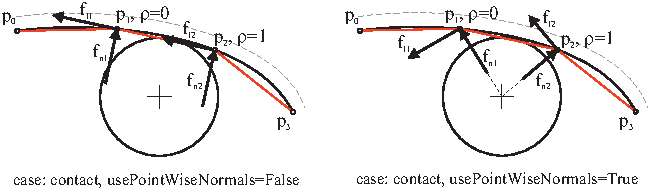
\includegraphics[width=16cm]{figures/ContactFrictionCircleCable2Dnormals.pdf}
      \end{center}
      \caption{Choice of normals and tangent vectors for calculation of normal contact forces and tangential (friction) forces; 
      note that the \texttt{useSegmentNormals=False} is not appropriate for this setup and would produce highly erroneous forces.}
        \label{fig:ObjectContactFrictionCircleCable2D:normals}
    \end{figure}
    }
    \onlyRST{
    .. _fig-objectcontactfrictioncirclecable2d-normals:
    .. figure:: docs/theDoc/figures/ContactFrictionCircleCable2Dnormals.png
       :width: 700

       Choice of normals and tangent vectors for calculation of normal contact forces and tangential (friction) forces; note that the \texttt{useSegmentNormals=False} is not appropriate for this setup and would produce highly erroneous forces.
    }
    %++++++++++++++++++++++++
    
    Segment normals (=SN) lead to always good approximations for normal directions, irrespectively of short or extremely long segments as compared to the circle. However, in case of segments that are short as compared to the circle radius, normals computed from the center of the circle to the segment points (=PWN) are more consistent and produce tangents only in circumferential direction, which may improve behavior in some applications. The equations for the two cases read:
    \bi
    \item[] \mybold{CASE SN}: use \mybold{S}egment \mybold{N}ormals\\
    If there is contact in a segment $s_i$, i.e., gap state $x_{gap} \le 0$, see \fig{fig:ObjectContactFrictionCircleCable2D:sketch}(right), contact forces $\fv_{s_i}$ are computed per segment,
    \be
      \fv_{s_i} = f_n \cdot \nv_{s_i} + f_t \tv_{s_i}
    \ee
    and added to every force at segment points according to
      \bea
        \fv_i &\pluseq& (1-\rho) \cdot \fv_{s_i}      \\ \nonumber
        \fv_{i+1} &\pluseq& \rho \cdot \fv_{s_i}
      \eea
    while in case $x_{gap}  > 0$ nothing is added.
    %     
    \item[] \mybold{CASE PWN}: use \mybold{P}oint \mybold{W}ise \mybold{N}ormals (at segment points)\\
    If there is contact in a segment $s_i$, i.e., gap $x_{gap} \le 0$, 
    see \fig{fig:ObjectContactFrictionCircleCable2D:sketch}(right), 
    intermediate contact forces $\fv^{l,r}_{i}$ are computed per segment point,
      \be
        \fv^l = f_n \cdot \nv_{l,s_i} + f_t \tv_{l,s_i}, \quad
        \fv^r = f_n \cdot \nv_{r,s_i} + f_t \tv_{r,s_i}
      \ee
      in which $\nv_{l,s_i}$ is the vector from circle center to the left point ($i$) of the segment $s_i$,
      and $\nv_{l,s_i}$ to the right point ($i+1$). The tangent vectors are perpendicular to the normals.
    %
      The forces are then applied to the contact forces $\fv_i$ using the parameter $\rho$, which takes into account the distance of contact to the left or right side of the segment,
      \bea
        \fv_i &\pluseq& (1-\rho) \cdot \fv^l      \\ \nonumber
        \fv_{i+1} &\pluseq& \rho \cdot \fv^r
      \eea
    while in case $x_{gap}  > 0$ nothing is added.
    \ei
    The forces $\fv_i$ are then applied through the marker to the \texttt{ObjectANCFCable2D} element as point loads via a position jacobian
    (using the according access function), for details see the C++ implementation.
    
    The forces on the circle marker $m0$ are computed as the total sum of all
    segment contact forces, 
    \be
      \fv_{m0} = -\sum_{s_i} \fv_{s_i} 
    \ee
    and additional torques on the circle's rotation simply follow from
    \be
      \tau_{m0} = -\sum_{s_i} r \cdot f_{t_{s_i}} \eqDot
    \ee
    %    
    During Newton iterations, the contact forces for segment $s_i$ are considered only, if 
    $x_i <= 0$. The dataCoordinate $x_i$ is not modified during Newton iterations, but computed
    during the DiscontinuousIteration, see \fig{fig_solver_discontinuous_iteration} in the solver description. 
    %
    \vspace{12pt}\\
    If \texttt{activeConnector = False}, all contact and friction forces on the cable and the force and torque on the 
    circle's marker are set to zero.
    %%RSTCOMPATIBLE
\vspace{6pt}\par\noindent\rule{\textwidth}{0.4pt}
%
\noindent For examples on ObjectContactFrictionCircleCable2D see Relevant Examples and TestModels with weblink:
\bi
\item \exuUrl{https://github.com/jgerstmayr/EXUDYN/blob/master/main/pythonDev/Examples/beltDriveALE.py}{\texttt{beltDriveALE.py}} (Examples/)
\item \exuUrl{https://github.com/jgerstmayr/EXUDYN/blob/master/main/pythonDev/Examples/beltDriveReevingSystem.py}{\texttt{beltDriveReevingSystem.py}} (Examples/)
\item \exuUrl{https://github.com/jgerstmayr/EXUDYN/blob/master/main/pythonDev/Examples/beltDrivesComparison.py}{\texttt{beltDrivesComparison.py}} (Examples/)
\item \exuUrl{https://github.com/jgerstmayr/EXUDYN/blob/master/main/pythonDev/Examples/sliderCrank3DwithANCFbeltDrive.py}{\texttt{sliderCrank3DwithANCFbeltDrive.py}} (Examples/)
\item \exuUrl{https://github.com/jgerstmayr/EXUDYN/blob/master/main/pythonDev/Examples/sliderCrank3DwithANCFbeltDrive2.py}{\texttt{sliderCrank3DwithANCFbeltDrive2.py}} (Examples/)
\item \exuUrl{https://github.com/jgerstmayr/EXUDYN/blob/master/main/pythonDev/TestModels/ANCFcontactFrictionTest.py}{\texttt{ANCFcontactFrictionTest.py}} (TestModels/)
\item \exuUrl{https://github.com/jgerstmayr/EXUDYN/blob/master/main/pythonDev/TestModels/ANCFmovingRigidBodyTest.py}{\texttt{ANCFmovingRigidBodyTest.py}} (TestModels/)
\item \exuUrl{https://github.com/jgerstmayr/EXUDYN/blob/master/main/pythonDev/TestModels/ANCFslidingAndALEjointTest.py}{\texttt{ANCFslidingAndALEjointTest.py}} (TestModels/)

\ei

%

\newpage
%+++++++++++++++++++++++++++++++
%+++++++++++++++++++++++++++++++
\mysubsection{Objects (Constraint)}
A Constraint is a special Object and Connector, which links two or more markers. A Constraint leads to algebraic equations, which exactly fulfill special constraints on the kinematic behavior of the multibody syste, such as a constraint on a coordinate or a distance constraint.
%++++++

%+++++++++++++++++++++++++++++++++++

\mysubsubsection{ObjectConnectorDistance}
\label{sec:item:ObjectConnectorDistance}
Connector which enforces constant or prescribed distance between two bodies/nodes.
\vspace{12pt}\\

\noindent \mybold{Additional information for ObjectConnectorDistance}:
\bi
  \item This \texttt{Object} has/provides the following types = \texttt{Connector}, \texttt{Constraint}
  \item Requested \texttt{Marker} type = \texttt{Position}
  \item {\bf Short name} for Python = \texttt{DistanceConstraint}
  \item {\bf Short name} for Python visualization object = \texttt{VDistanceConstraint}
\ei\vspace{12pt} \noindent 
The item \mybold{ObjectConnectorDistance} with type = 'ConnectorDistance' has the following parameters:
\vspace{-0.5cm}\\
\vspace{-0.5cm}\\
%reference manual TABLE
\begin{center}
  \footnotesize
  \begin{longtable}{| p{4.5cm} | p{2.5cm} | p{0.5cm} | p{2.5cm} | p{6cm} |}
    \hline
    \bf Name & \bf type & \bf size & \bf default value & \bf description \\ \hline
    name &     String &      &     '' &     constraints's unique name\\ \hline
    markerNumbers &     ArrayMarkerIndex &     \tabnewline  &     [ invalid [-1], invalid [-1] ] &     \tabnewline list of markers used in connector\\ \hline
    distance &     PReal &      &     0. &     prescribed distance [SI:m] of the used markers; must by greater than zero\\ \hline
    activeConnector &     Bool &      &     True &     flag, which determines, if the connector is active; used to deactivate (temporarily) a connector or constraint\\ \hline
    visualization &     VObjectConnectorDistance &      &      &     parameters for visualization of item\\ \hline
\end{longtable}
\end{center}

\noindent The item VObjectConnectorDistance has the following parameters:
%reference manual TABLE
\begin{center}
  \footnotesize
  \begin{longtable}{| p{4.5cm} | p{2.5cm} | p{0.5cm} | p{2.5cm} | p{6cm} |}
    \hline
    \bf Name & \bf type & \bf size & \bf default value & \bf description \\ \hline
    show &     Bool &      &     True &     set true, if item is shown in visualization and false if it is not shown\\ \hline
    drawSize &     float &      &     -1. &     drawing size = link size; size == -1.f means that default connector size is used\\ \hline
    color &     Float4 &      &     [-1.,-1.,-1.,-1.] &     \tabnewline RGBA connector color; if R==-1, use default color\\ \hline
\end{longtable}
\end{center}
\par\noindent\rule{\textwidth}{0.4pt}
\mysubsubsubsection{DESCRIPTION of ObjectConnectorDistance:}
\label{description_ObjectConnectorDistance}
\paragraph{Information on input parameters:} 
\startTable{input parameter}{symbol}{description see tables above}
\rowTable{markerNumbers}{$[m0,m1]\tp$}{}
\rowTable{distance}{$d_0$}{}
\finishTable

\mybold{The following output variables are available as OutputVariableType in sensors, Get...Output() and other functions}:
\begin{center}
\footnotesize
\begin{longtable}{| p{5cm} | p{5cm} | p{6cm} |} 
\hline
\bf output variable & \bf symbol & \bf description \\ \hline
Displacement & $\LU{0}{\Delta\pv}$ & relative displacement in global coordinates\\ \hline
Velocity & $\LU{0}{\Delta\vv}$ & relative translational velocity in global coordinates\\ \hline
Distance & $|\LU{0}{\Delta\pv}|$ & distance between markers (should stay constant; shows constraint deviation)\\ \hline
Force & $\lambda_0$ & joint force (=scalar Lagrange multiplier)\\ \hline
\end{longtable}
\end{center}
 \noindent
    \mysubsubsubsection{Definition of quantities}
    \startTable{intermediate variables}{symbol}{description}
        \rowTable{marker m0 position}{$\LU{0}{\pv}_{m0}$}{current global position which is provided by marker m0}
        \rowTable{marker m1 position}{$\LU{0}{\pv}_{m1}$}{accordingly}
    %
        \rowTable{marker m0 velocity}{$\LU{0}{\vv}_{m0}$}{current global velocity which is provided by marker m0}
        \rowTable{marker m1 velocity}{$\LU{0}{\vv}_{m1}$}{accordingly}
        \rowTable{relative displacement}{$\LU{0}{\Delta\pv}$}{$\LU{0}{\pv}_{m1} - \LU{0}{\pv}_{m0}$}
        \rowTable{relative velocity}{$\LU{0}{\Delta\vv}$}{$\LU{0}{\vv}_{m1} - \LU{0}{\vv}_{m0}$}
    %
        \rowTable{algebraicVariable}{$\lambda_0$}{Lagrange multiplier = force in constraint}
    \finishTable

    \mysubsubsubsection{Connector forces constraint equations}
    If \texttt{activeConnector = True}, the index 3 algebraic equation reads
    \be
      \left|\LU{0}{\Delta\pv}\right| - d_0 = 0
    \ee
    Due to the fact that the force direction is given by
    \be
      \frac{1}{|\LU{0}{\Delta\pv}|}\LU{0}{\Delta\pv} \eqComma
    \ee
    the prescribed distance $d_0$ may not be zero. This would, otherwise, result in a change of the number of constraints.
    The index 2 (velocity level) algebraic equation reads
    \be
      \left(\frac{\LU{0}{\Delta\pv}}{\left|\LU{0}{\Delta\pv}\right|}\right)\tp \Delta\vv = 0
    \ee
    if \texttt{activeConnector = False}, the algebraic equation reads
    \be
      \lambda_0 = 0
    \ee
    %%RSTCOMPATIBLE
\vspace{6pt}\par\noindent\rule{\textwidth}{0.4pt}
\mysubsubsubsection{MINI EXAMPLE for ObjectConnectorDistance}
\label{miniExample_ObjectConnectorDistance}
\pythonstyle
\begin{lstlisting}[language=Python, firstnumber=1]
    #example with 1m pendulum, 50kg under gravity
    nMass = mbs.AddNode(NodePoint2D(referenceCoordinates=[1,0]))
    oMass = mbs.AddObject(MassPoint2D(physicsMass = 50, nodeNumber = nMass))
    
    mMass = mbs.AddMarker(MarkerNodePosition(nodeNumber=nMass))
    mGround = mbs.AddMarker(MarkerBodyPosition(bodyNumber=oGround, localPosition = [0,0,0]))
    oDistance = mbs.AddObject(DistanceConstraint(markerNumbers = [mGround, mMass], distance = 1))
    
    mbs.AddLoad(Force(markerNumber = mMass, loadVector = [0, -50*9.81, 0])) 

    #assemble and solve system for default parameters
    mbs.Assemble()
    
    sims=exu.SimulationSettings()
    sims.timeIntegration.generalizedAlpha.spectralRadius=0.7
    mbs.SolveDynamic(sims)

    #check result at default integration time
    exudynTestGlobals.testResult = mbs.GetNodeOutput(nMass, exu.OutputVariableType.Position)[0]
\end{lstlisting}

\vspace{6pt}\par\noindent\rule{\textwidth}{0.4pt}
%
\noindent For examples on ObjectConnectorDistance see Relevant Examples and TestModels with weblink:
\bi
\item \exuUrl{https://github.com/jgerstmayr/EXUDYN/blob/master/main/pythonDev/Examples/HydraulicActuatorStaticInitialization.py}{\texttt{HydraulicActuatorStaticInitialization.py}} (Examples/)
\item \exuUrl{https://github.com/jgerstmayr/EXUDYN/blob/master/main/pythonDev/Examples/pendulum2Dconstraint.py}{\texttt{pendulum2Dconstraint.py}} (Examples/)
\item \exuUrl{https://github.com/jgerstmayr/EXUDYN/blob/master/main/pythonDev/Examples/pendulumIftommBenchmark.py}{\texttt{pendulumIftommBenchmark.py}} (Examples/)
\item \exuUrl{https://github.com/jgerstmayr/EXUDYN/blob/master/main/pythonDev/TestModels/fourBarMechanismTest.py}{\texttt{fourBarMechanismTest.py}} (TestModels/)
\item \exuUrl{https://github.com/jgerstmayr/EXUDYN/blob/master/main/pythonDev/TestModels/coordinateVectorConstraint.py}{\texttt{coordinateVectorConstraint.py}} (TestModels/)
\item \exuUrl{https://github.com/jgerstmayr/EXUDYN/blob/master/main/pythonDev/TestModels/coordinateVectorConstraintGenericODE2.py}{\texttt{coordinateVectorConstraintGenericODE2.py}} (TestModels/)
\item \exuUrl{https://github.com/jgerstmayr/EXUDYN/blob/master/main/pythonDev/TestModels/modelUnitTests.py}{\texttt{modelUnitTests.py}} (TestModels/)
\item \exuUrl{https://github.com/jgerstmayr/EXUDYN/blob/master/main/pythonDev/TestModels/PARTS_ATEs_moving.py}{\texttt{PARTS\_ATEs\_moving.py}} (TestModels/)

\ei

%
\newpage

%+++++++++++++++++++++++++++++++++++

\mysubsubsection{ObjectConnectorCoordinate}
\label{sec:item:ObjectConnectorCoordinate}
A coordinate constraint which constrains two (scalar) coordinates of Marker[Node|Body]Coordinates attached to nodes or bodies. The constraint acts directly on coordinates, but does not include reference values, e.g., of nodal values. This constraint is computationally efficient and should be used to constrain nodal coordinates.
\vspace{12pt}\\

\noindent \mybold{Additional information for ObjectConnectorCoordinate}:
\bi
  \item This \texttt{Object} has/provides the following types = \texttt{Connector}, \texttt{Constraint}
  \item Requested \texttt{Marker} type = \texttt{Coordinate}
  \item {\bf Short name} for Python = \texttt{CoordinateConstraint}
  \item {\bf Short name} for Python visualization object = \texttt{VCoordinateConstraint}
\ei\vspace{12pt} \noindent 
The item \mybold{ObjectConnectorCoordinate} with type = 'ConnectorCoordinate' has the following parameters:
\vspace{-0.5cm}\\
\vspace{-0.5cm}\\
%reference manual TABLE
\begin{center}
  \footnotesize
  \begin{longtable}{| p{4.5cm} | p{2.5cm} | p{0.5cm} | p{2.5cm} | p{6cm} |}
    \hline
    \bf Name & \bf type & \bf size & \bf default value & \bf description \\ \hline
    name &     String &      &     '' &     constraints's unique name\\ \hline
    markerNumbers &     ArrayMarkerIndex &     \tabnewline  &     [ invalid [-1], invalid [-1] ] &     \tabnewline list of markers used in connector\\ \hline
    offset &     Real &      &     0. &     An offset between the two values\\ \hline
    factorValue1 &     Real &      &     1. &     An additional factor multiplied with value1 used in algebraic equation\\ \hline
    velocityLevel &     Bool &      &     False &     If true: connector constrains velocities (only works for \hac{ODE2} coordinates!); offset is used between velocities; in this case, the offsetUserFunction\_t is considered and offsetUserFunction is ignored\\ \hline
    offsetUserFunction &     PyFunctionMbsScalarIndexScalar &     \tabnewline  &     \tabnewline 0 &     A Python function which defines the time-dependent offset; see description below\\ \hline
    offsetUserFunction\_t &     PyFunctionMbsScalarIndexScalar &     \tabnewline  &     \tabnewline 0 &     time derivative of offsetUserFunction; needed for velocity level constraints; see description below\\ \hline
    activeConnector &     Bool &      &     True &     flag, which determines, if the connector is active; used to deactivate (temporarily) a connector or constraint\\ \hline
    visualization &     VObjectConnectorCoordinate &      &      &     parameters for visualization of item\\ \hline
\end{longtable}
\end{center}

\noindent The item VObjectConnectorCoordinate has the following parameters:
%reference manual TABLE
\begin{center}
  \footnotesize
  \begin{longtable}{| p{4.5cm} | p{2.5cm} | p{0.5cm} | p{2.5cm} | p{6cm} |}
    \hline
    \bf Name & \bf type & \bf size & \bf default value & \bf description \\ \hline
    show &     Bool &      &     True &     set true, if item is shown in visualization and false if it is not shown\\ \hline
    drawSize &     float &      &     -1. &     drawing size = link size; size == -1.f means that default connector size is used\\ \hline
    color &     Float4 &      &     [-1.,-1.,-1.,-1.] &     \tabnewline RGBA connector color; if R==-1, use default color\\ \hline
\end{longtable}
\end{center}
\par\noindent\rule{\textwidth}{0.4pt}
\mysubsubsubsection{DESCRIPTION of ObjectConnectorCoordinate:}
\label{description_ObjectConnectorCoordinate}
\paragraph{Information on input parameters:} 
\startTable{input parameter}{symbol}{description see tables above}
\rowTable{markerNumbers}{$[m0,m1]\tp$}{}
\rowTable{offset}{$l_\mathrm{off}$}{}
\rowTable{factorValue1}{$k_{m1}$}{}
\rowTable{offsetUserFunction}{$\mathrm{UF} \in \Rcal$}{}
\rowTable{offsetUserFunction\_t}{$\mathrm{UF}_t \in \Rcal$}{}
\finishTable

\mybold{The following output variables are available as OutputVariableType in sensors, Get...Output() and other functions}:
\begin{center}
\footnotesize
\begin{longtable}{| p{5cm} | p{5cm} | p{6cm} |} 
\hline
\bf output variable & \bf symbol & \bf description \\ \hline
Displacement & $\Delta q$ & relative scalar displacement of marker coordinates, not including factorValue1\\ \hline
Velocity & $\Delta v$ & difference of scalar marker velocity coordinates, not including factorValue1\\ \hline
ConstraintEquation & $\cv$ & (residuum of) constraint equation\\ \hline
Force & $\lambda_0$ & scalar constraint force (Lagrange multiplier)\\ \hline
\end{longtable}
\end{center}
 \noindent
    \mysubsubsubsection{Definition of quantities}
    \startTable{intermediate variables}{symbol}{description}
    \rowTable{marker m0 coordinate}{$q_{m0}$}{current displacement coordinate which is provided by marker m0; does NOT include reference coordinate!}
    \rowTable{marker m1 coordinate}{$q_{m1}$}{}
    \rowTable{marker m0 velocity coordinate}{$v_{m0}$}{current velocity coordinate which is provided by marker m0}
    \rowTable{marker m1 velocity coordinate}{$v_{m1}$}{}
    \rowTable{difference of coordinates}{$\Delta q = q_{m1} - q_{m0}$}{Displacement between marker m0 to marker m1 coordinates (does NOT include reference coordinates)}
    \rowTable{difference of velocity coordinates}{$\Delta v= v_{m1} - v_{m0}$}{}
    \finishTable
    \mysubsubsubsection{Connector constraint equations}
    If \texttt{activeConnector = True}, the index 3 algebraic equation reads
    \be
      \cv(q_{m0}, q_{m1}) = k_{m1} \cdot q_{m1} - q_{m0} - l_\mathrm{off} = 0
    \ee
    If the offsetUserFunction $\mathrm{UF}$ is defined, $\cv$ instead becomes ($t$ is current time)
    \be
      \cv(q_{m0}, q_{m1}) = k_{m1} \cdot q_{m1} - q_{m0} -  \mathrm{UF}(mbs, t, i_N, l_\mathrm{off}) = 0
    \ee
    The \texttt{activeConnector = True}, index 2 (velocity level) algebraic equation reads
    \be
      \dot \cv(\dot q_{m0}, \dot q_{m1}) = k_{m1} \cdot \dot q_{m1} - \dot q_{m0} - d = 0
    \ee
    The factor $d$ in velocity level equations is zero, except if parameters.velocityLevel = True, then $d=l_\mathrm{off}$.
    If velocity level constraints are active and the velocity level offsetUserFunction\_t $\mathrm{UF}_t$ is defined, $\dot \cv$ instead becomes ($t$ is current time)
    \be
      \dot \cv(\dot q_{m0}, \dot q_{m1}) = k_{m1} \cdot \dot q_{m1} - \dot q_{m0} - \mathrm{UF}_t(mbs, t, i_N, l_\mathrm{off}) = 0
    \ee
    and \texttt{iN} represents the itemNumber (=objectNumber).
    Note that the index 2 equations are used, if the solver uses index 2 formulation OR if the flag parameters.velocityLevel = True (or both).
    The user functions include dependency on time $t$, but this time dependency is not respected in the computation of initial accelerations. Therefore,
    it is recommended that $\mathrm{UF}$ and $\mathrm{UF}_t$ does not include initial accelerations.

    If \texttt{activeConnector = False}, the (index 1) algebraic equation reads for ALL cases:
    \be
      \cv(\lambda_0) = \lambda_0 = 0
    \ee
    %
    %++++++++++++++++++++++++++++++++++++++++++++++++++++++++++
    \userFunction{offsetUserFunction(mbs, t, itemNumber, lOffset)}
    %
    A user function, which computes scalar offset for the coordinate constraint, e.g., in order to move a node on a prescribed trajectory.
    It is NECESSARY to use sufficiently smooth functions, having {\bf initial offsets} consistent with {\bf initial configuration} of bodies, 
    either zero or compatible initial offset-velocity, and no initial accelerations.
    The \texttt{offsetUserFunction} is {\bf ONLY used} in case of static computation or index3 (generalizedAlpha) time integration.
    In order to be on the safe side, provide both  \texttt{offsetUserFunction} and  \texttt{offsetUserFunction\_t}.

    Note that itemNumber represents the index of the object in mbs, which can be used to retrieve additional data from the object through
    \texttt{mbs.GetObjectParameter(itemNumber, ...)}, see the according description of \texttt{GetObjectParameter}.

    The user function gets time and the offset parameter as an input and returns the computed offset:
    %
    \startTable{arguments / return}{type or size}{description}
      \rowTable{\texttt{mbs}}{MainSystem}{provides MainSystem mbs in which underlying item is defined}
      \rowTable{\texttt{t}}{Real}{current time in mbs} %use t instead time in order to avoid possible conflicts with Python time
      \rowTable{\texttt{itemNumber}}{Index}{integer number $i_N$ of the object in mbs, allowing easy access to all object data via mbs.GetObjectParameter(itemNumber, ...)}
      \rowTable{\texttt{lOffset}}{Real}{$l_\mathrm{off}$}
      \rowTable{\returnValue}{Real}{computed offset for given time}
    \finishTable
    %
    %++++++++++++++++++++++++++++++++++++++++++++++++++++++++++
    \userFunction{offsetUserFunction\_t(mbs, t, itemNumber, lOffset)}
    %
    A user function, which computes scalar offset {\bf velocity} for the coordinate constraint.
    It is NECESSARY to use sufficiently smooth functions, having {\bf initial offset velocities} consistent with {\bf initial velocities} of bodies.
    The \texttt{offsetUserFunction\_t} is used instead of \texttt{offsetUserFunction} in case of \texttt{velocityLevel = True}, 
    or for index2 time integration and needed for computation of initial accelerations in second order implicit time integrators.

    Note that itemNumber represents the index of the object in mbs, which can be used to retrieve additional data from the object through
    \texttt{mbs.GetObjectParameter(itemNumber, ...)}, see the according description of \texttt{GetObjectParameter}.

    The user function gets time and the offset parameter as an input and returns the computed offset velocity:
    %
    \startTable{arguments / return}{type or size}{description}
      \rowTable{\texttt{mbs}}{MainSystem}{provides MainSystem mbs in which underlying item is defined}
      \rowTable{\texttt{t}}{Real}{current time in mbs} %use t instead time in order to avoid possible conflicts with Python time
      \rowTable{\texttt{itemNumber}}{Index}{integer number of the object in mbs, allowing easy access to all object data via mbs.GetObjectParameter(itemNumber, ...)}
      \rowTable{\texttt{lOffset}}{Real}{$l_\mathrm{off}$}
      \rowTable{\returnValue}{Real}{computed offset velocity for given time}
    \finishTable
    %
    %++++++++++++++++++++++++++++++++++++++++++++++++++++++++++
    \userFunctionExample{}
    \pythonstyle\begin{lstlisting}
        #see also mini example!
        from math import sin, cos, pi
        def UFoffset(mbs, t, itemNumber, lOffset): 
            return 0.5*lOffset*(1-cos(0.5*pi*t))
        
        def UFoffset_t(mbs, t, itemNumber, lOffset): #time derivative of UFoffset
            return 0.5*lOffset*0.5*pi*sin(0.5*pi*t)

        nMass=mbs.AddNode(Point(referenceCoordinates = [2,0,0]))
        massPoint = mbs.AddObject(MassPoint(physicsMass = 5, nodeNumber = nMass))
        
        groundMarker=mbs.AddMarker(MarkerNodeCoordinate(nodeNumber= nGround, coordinate = 0))
        nodeMarker  =mbs.AddMarker(MarkerNodeCoordinate(nodeNumber= nMass, coordinate = 0))
        
        #Spring-Damper between two marker coordinates
        mbs.AddObject(CoordinateConstraint(markerNumbers = [groundMarker, nodeMarker], 
                                           offset = 0.1, 
                                           offsetUserFunction = UFoffset, 
                                           offsetUserFunction_t = UFoffset_t)) 
    \end{lstlisting}
    %%RSTCOMPATIBLE
\vspace{6pt}\par\noindent\rule{\textwidth}{0.4pt}
\mysubsubsubsection{MINI EXAMPLE for ObjectConnectorCoordinate}
\label{miniExample_ObjectConnectorCoordinate}
\pythonstyle
\begin{lstlisting}[language=Python, firstnumber=1]
    def OffsetUF(mbs, t, itemNumber, lOffset): #gives 0.05 at t=1
        return 0.5*(1-np.cos(2*3.141592653589793*0.25*t))*lOffset

    nMass=mbs.AddNode(Point(referenceCoordinates = [2,0,0]))
    massPoint = mbs.AddObject(MassPoint(physicsMass = 5, nodeNumber = nMass))
    
    groundMarker=mbs.AddMarker(MarkerNodeCoordinate(nodeNumber= nGround, coordinate = 0))
    nodeMarker  =mbs.AddMarker(MarkerNodeCoordinate(nodeNumber= nMass, coordinate = 0))
    
    #Spring-Damper between two marker coordinates
    mbs.AddObject(CoordinateConstraint(markerNumbers = [groundMarker, nodeMarker], 
                                       offset = 0.1, offsetUserFunction = OffsetUF)) 

    #assemble and solve system for default parameters
    mbs.Assemble()
    mbs.SolveDynamic()

    #check result at default integration time
    exudynTestGlobals.testResult  = mbs.GetNodeOutput(nMass, exu.OutputVariableType.Displacement)[0]
\end{lstlisting}

\vspace{6pt}\par\noindent\rule{\textwidth}{0.4pt}
%
\noindent For examples on ObjectConnectorCoordinate see Relevant Examples and TestModels with weblink:
\bi
\item \exuUrl{https://github.com/jgerstmayr/EXUDYN/blob/master/main/pythonDev/Examples/sliderCrank3DwithANCFbeltDrive2.py}{\texttt{sliderCrank3DwithANCFbeltDrive2.py}} (Examples/)
\item \exuUrl{https://github.com/jgerstmayr/EXUDYN/blob/master/main/pythonDev/Examples/ALEANCFpipe.py}{\texttt{ALEANCFpipe.py}} (Examples/)
\item \exuUrl{https://github.com/jgerstmayr/EXUDYN/blob/master/main/pythonDev/Examples/ANCFALEtest.py}{\texttt{ANCFALEtest.py}} (Examples/)
\item \exuUrl{https://github.com/jgerstmayr/EXUDYN/blob/master/main/pythonDev/Examples/ANCFcantileverTestDyn.py}{\texttt{ANCFcantileverTestDyn.py}} (Examples/)
\item \exuUrl{https://github.com/jgerstmayr/EXUDYN/blob/master/main/pythonDev/Examples/ANCFcontactCircle.py}{\texttt{ANCFcontactCircle.py}} (Examples/)
\item \exuUrl{https://github.com/jgerstmayr/EXUDYN/blob/master/main/pythonDev/Examples/ANCFcontactCircle2.py}{\texttt{ANCFcontactCircle2.py}} (Examples/)
\item \exuUrl{https://github.com/jgerstmayr/EXUDYN/blob/master/main/pythonDev/Examples/ANCFmovingRigidbody.py}{\texttt{ANCFmovingRigidbody.py}} (Examples/)
\item \exuUrl{https://github.com/jgerstmayr/EXUDYN/blob/master/main/pythonDev/Examples/ANCFrotatingCable2D.py}{\texttt{ANCFrotatingCable2D.py}} (Examples/)
\item \exuUrl{https://github.com/jgerstmayr/EXUDYN/blob/master/main/pythonDev/Examples/ANCFslidingJoint2D.py}{\texttt{ANCFslidingJoint2D.py}} (Examples/)
\item \exuUrl{https://github.com/jgerstmayr/EXUDYN/blob/master/main/pythonDev/Examples/ANCFslidingJoint2Drigid.py}{\texttt{ANCFslidingJoint2Drigid.py}} (Examples/)
\item \exuUrl{https://github.com/jgerstmayr/EXUDYN/blob/master/main/pythonDev/Examples/ANCFswitchingSlidingJoint2D.py}{\texttt{ANCFswitchingSlidingJoint2D.py}} (Examples/)
\item \exuUrl{https://github.com/jgerstmayr/EXUDYN/blob/master/main/pythonDev/Examples/ANCFtestHalfcircle.py}{\texttt{ANCFtestHalfcircle.py}} (Examples/)
\item  ...

\item \exuUrl{https://github.com/jgerstmayr/EXUDYN/blob/master/main/pythonDev/TestModels/ANCFBeamTest.py}{\texttt{ANCFBeamTest.py}} (TestModels/)
\item \exuUrl{https://github.com/jgerstmayr/EXUDYN/blob/master/main/pythonDev/TestModels/ANCFbeltDrive.py}{\texttt{ANCFbeltDrive.py}} (TestModels/)
\item \exuUrl{https://github.com/jgerstmayr/EXUDYN/blob/master/main/pythonDev/TestModels/ANCFcontactCircleTest.py}{\texttt{ANCFcontactCircleTest.py}} (TestModels/)
\item  ...


\ei

%
\newpage

%+++++++++++++++++++++++++++++++++++

\mysubsubsection{ObjectConnectorCoordinateVector}
\label{sec:item:ObjectConnectorCoordinateVector}
A constraint which constrains the coordinate vectors of two markers Marker[Node|Object|Body]Coordinates attached to nodes or bodies. The marker uses the objects \ac{LTG}-lists to build the according coordinate mappings.
\vspace{12pt}\\

\noindent \mybold{Additional information for ObjectConnectorCoordinateVector}:
\bi
  \item This \texttt{Object} has/provides the following types = \texttt{Connector}, \texttt{Constraint}
  \item Requested \texttt{Marker} type = \texttt{Coordinate}
  \item {\bf Short name} for Python = \texttt{CoordinateVectorConstraint}
  \item {\bf Short name} for Python visualization object = \texttt{VCoordinateVectorConstraint}
\ei\vspace{12pt} \noindent 
The item \mybold{ObjectConnectorCoordinateVector} with type = 'ConnectorCoordinateVector' has the following parameters:
\vspace{-0.5cm}\\
\vspace{-0.5cm}\\
%reference manual TABLE
\begin{center}
  \footnotesize
  \begin{longtable}{| p{4.5cm} | p{2.5cm} | p{0.5cm} | p{2.5cm} | p{6cm} |}
    \hline
    \bf Name & \bf type & \bf size & \bf default value & \bf description \\ \hline
    name &     String &      &     '' &     constraints's unique name\\ \hline
    markerNumbers &     ArrayMarkerIndex &     \tabnewline  &     [ invalid [-1], invalid [-1] ] &     \tabnewline list of markers used in connector\\ \hline
    scalingMarker0 &     NumpyMatrix &      &     Matrix[] &     linear scaling matrix for coordinate vector of marker 0; matrix provided in Python numpy format\\ \hline
    scalingMarker1 &     NumpyMatrix &      &     Matrix[] &     linear scaling matrix for coordinate vector of marker 1; matrix provided in Python numpy format\\ \hline
    quadraticTermMarker0 &     NumpyMatrix &      &     Matrix[] &     quadratic scaling matrix for coordinate vector of marker 0; matrix provided in Python numpy format\\ \hline
    quadraticTermMarker1 &     NumpyMatrix &      &     Matrix[] &     quadratic scaling matrix for coordinate vector of marker 1; matrix provided in Python numpy format\\ \hline
    offset &     NumpyVector &      &     [] &     offset added to constraint equation; only active, if no userFunction is defined\\ \hline
    velocityLevel &     Bool &      &     False &     If true: connector constrains velocities (only works for \hac{ODE2} coordinates!); offset is used between velocities; in this case, the offsetUserFunction\_t is considered and offsetUserFunction is ignored\\ \hline
    constraintUserFunction &     PyFunctionVectorMbsScalarIndex2VectorBool &     \tabnewline  &     \tabnewline 0 &     \tabnewline A Python user function which computes the constraint equations; to define the number of algebraic equations, set scalingMarker0 as a numpy.zeros((nAE,1)) array with nAE being the number algebraic equations; see description below\\ \hline
    jacobianUserFunction &     PyFunctionMatrixContainerMbsScalarIndex2VectorBool &     \tabnewline  &     \tabnewline 0 &     \tabnewline A Python user function which computes the jacobian, i.e., the derivative of the left-hand-side object equation w.r.t.\ the coordinates (times $f_{ODE2}$) and w.r.t.\ the velocities (times $f_{ODE2_t}$). Terms on the RHS must be subtracted from the LHS equation; the respective terms for the stiffness matrix and damping matrix are automatically added; see description below\\ \hline
    activeConnector &     Bool &      &     True &     flag, which determines, if the connector is active; used to deactivate (temporarily) a connector or constraint\\ \hline
    visualization &     VObjectConnectorCoordinateVector &      &      &     parameters for visualization of item\\ \hline
\end{longtable}
\end{center}

\noindent The item VObjectConnectorCoordinateVector has the following parameters:
%reference manual TABLE
\begin{center}
  \footnotesize
  \begin{longtable}{| p{4.5cm} | p{2.5cm} | p{0.5cm} | p{2.5cm} | p{6cm} |}
    \hline
    \bf Name & \bf type & \bf size & \bf default value & \bf description \\ \hline
    show &     Bool &      &     True &     set true, if item is shown in visualization and false if it is not shown\\ \hline
    color &     Float4 &      &     [-1.,-1.,-1.,-1.] &     \tabnewline RGBA connector color; if R==-1, use default color\\ \hline
\end{longtable}
\end{center}
\par\noindent\rule{\textwidth}{0.4pt}
\mysubsubsubsection{DESCRIPTION of ObjectConnectorCoordinateVector:}
\label{description_ObjectConnectorCoordinateVector}
\paragraph{Information on input parameters:} 
\startTable{input parameter}{symbol}{description see tables above}
\rowTable{markerNumbers}{$[m0,m1]\tp$}{}
\rowTable{scalingMarker0}{$\Xm_{m0} \in \Rcal^{n_{ae} \times n_{q_{m0}}}$}{}
\rowTable{scalingMarker1}{$\Xm_{m1} \in \Rcal^{n_{ae} \times n_{q_{m1}}}$}{}
\rowTable{quadraticTermMarker0}{$\Ym_{m0} \in \Rcal^{n_{ae} \times n_{q_{m0}}}$}{}
\rowTable{quadraticTermMarker1}{$\Ym_{m0} \in \Rcal^{n_{ae} \times n_{q_{m0}}}$}{}
\rowTable{offset}{$\vv_\mathrm{off} \in \Rcal^{n_{ae}}$}{}
\rowTable{constraintUserFunction}{$\cv_{user} \in \Rcal^{n_{ae}}$}{}
\rowTable{jacobianUserFunction}{$\Jm_{user} \in \Rcal^{(n_{q_{m0}}+n_{q_{m1}}) \times n_{ae}}$}{}
\finishTable

\mybold{The following output variables are available as OutputVariableType in sensors, Get...Output() and other functions}:
\begin{center}
\footnotesize
\begin{longtable}{| p{5cm} | p{5cm} | p{6cm} |} 
\hline
\bf output variable & \bf symbol & \bf description \\ \hline
Displacement & $\Delta \qv$ & relative scalar displacement of marker coordinates, not including scaling matrices\\ \hline
Velocity & $\Delta \vv$ & difference of scalar marker velocity coordinates, not including scaling matrices\\ \hline
ConstraintEquation & $\cv$ & (residuum of) constraint equations\\ \hline
Force & $\tlambda$ & constraint force vector (vector of Lagrange multipliers), resulting from action of constraint equations\\ \hline
\end{longtable}
\end{center}
 \noindent
    \mysubsubsubsection{Definition of quantities}
    \startTable{intermediate variables}{symbol}{description}
    \rowTable{marker m0 coordinate vector}{$\qv_{m0} \in \Rcal^{n_{q_{m0}}}$}{coordinate vector provided by marker $m0$; depending on the marker, the coordinates may or may not include reference coordinates}
    \rowTable{marker m1 coordinate vector}{$\qv_{m1} \in \Rcal^{n_{q_{m1}}}$}{coordinate vector provided by marker $m1$; depending on the marker, the coordinates may or may not include reference coordinates}
    \rowTable{marker m0 velocity coordinate vector}{$\dot \qv_{m0} \in \Rcal^{n_{q_{m0}}}$}{velocity coordinate vector provided by marker $m0$}
    \rowTable{marker m1 velocity coordinate vector}{$\dot \qv_{m1} \in \Rcal^{n_{q_{m1}}}$}{velocity coordinate vector provided by marker $m1$}
    \rowTable{number of algebraic equations}{$n_{ae}$}{number of algebraic equations must be same as number of rows in $\Xm_{m0}$ and $\Xm_{m1}$}
    %
    \rowTable{difference of coordinates}{$\Delta \qv = \qv_{m1} - \qv_{m0}$}{Displacement between marker m0 to marker m1 coordinates}
    \rowTable{difference of velocity coordinates}{$\Delta \vv= \dot \qv_{m1} - \dot \qv_{m0}$}{}
    \finishTable
    %
    \mysubsubsubsection{Remarks}
    The number of algebraic equations depends on the maximum number of rows in $\Xm_{m0}$, $\Ym_{m0}$, $\Xm_{m1}$ and $\Ym_{m1}$. 
    The number of rows of the latter matrices must either be zero or the maximum of these rows.

    The number of columns in $\Xm_{m0}$ (or $\Ym_{m0}$) must agree with the length of the coordinate vector
    $\qv_{m0}$ and the number of columns in $\Xm_{m1}$ (or $\Ym_{m1}$) must agree with the length of the coordinate vector
    $\qv_{m1}$, if these matrices are not empty matrices. 
    If one marker $k$ is a ground marker (node/object), the length of $\qv_{m,k}$ is zero and also the according matrices
    $\Xm_{m,k}$, $\Ym_{m,k}$  have zero size and will not be considered in the computation of the constraint equations.

    %If the number of rows of $\Xm_{m0}$ plus the number of rows of $\Xm_{m1}$ is
    %larger than the total number of coordinates ( $\qv_{m0}$ and  $\qv_{m1}$), the algebraic equations are 
    %underdetermined and probably not solvable.

    \mysubsubsubsection{Connector constraint equations}
    If \texttt{activeConnector = True} and no \texttt{constraintUserFunction} is defined, the index 3 algebraic equations
    \be
      \cv(\qv_{m0}, \qv_{m1}) = \Xm_{m1} \cdot \qv_{m1} 
      + \Ym_{m1} \cdot \qv^2_{m1} %quadratic terms have been excluded, as it could not be used for Euler Parameter constraints!
      - \Xm_{m0} \cdot\qv_{m0} 
      - \Ym_{m0} \cdot\qv^2_{m0} 
      - \vv_\mathrm{off} = 0
    \ee
    Note that the squared coordinates are understood as $\qv^2_{m0} = [q^2_{0,m0}, \; q^2_{1,m0}, \; \ldots]\tp$, same for $\qv^2_{m1}$.

    The index 2 (velocity level) algebraic equation accordingly reads
    \be
      \dot \cv(\dot \qv_{m0}, \dot \qv_{m1}) = \Xm_{m1} \cdot \dot \qv_{m1} 
      + \Ym_{m1} \cdot \dot \qv^2_{m1} 
      - \Xm_{m0} \cdot \dot \qv_{m0} 
      - \Ym_{m0} \cdot \dot \qv^2_{m0} 
      - \dv_\mathrm{off} = 0
    \ee
    The vector $\dv$ in velocity level equations is zero, except if \texttt{parameters.velocityLevel = True}, then $\dv=\vv_\mathrm{off}$.

    Note that the index 2 equations are used, if the solver uses index 2 formulation OR if the flag \texttt{parameters.velocityLevel = True} (or both).
    However, the \texttt{constraintUserFunction} has to be chosen accordingly by the user, either as position or as velocity level.
    The user functions include dependency on time $t$, but this time dependency is not respected in the computation of initial accelerations. Therefore,

    If \texttt{activeConnector = False}, the (index 1) algebraic equation reads for ALL cases:
    \be
      \cv(\tlambda) = \tlambda = 0
    \ee


    If a \texttt{constraintUserFunction} is defined, it also requires an according \texttt{jacobianUserFunction} (and vice versa).
    %without $\Km$ and $\Dm$ (these matrices are added internally),
    %\be \label{eq_ObjectGenericODE2_Jac}
    %  \Jm_{user}(mbs, t, i_N, \qv, \dot \qv, f_{ODE2}, f_{ODE2_t}) =
    %        -f_{ODE2}   \left(\frac{\partial \fv_{user}(mbs, t, i_N,\qv,\dot \qv)}{\partial \qv} \right) - 
    %         f_{ODE2_t} \left(\frac{\partial \fv_{user}(mbs, t, i_N,\qv,\dot \qv)}{\partial \dot \qv} \right)
    %\ee
    %CoordinateLoads are added for the respective \hac{ODE2} coordinate on the RHS of the latter equation.
    %
    %++++++++++++++++++++++++++++++++++++++++++++++++++++++++++
    \userFunction{constraintUserFunction(mbs, t, itemNumber, q, q\_t, velocityLevel)}
    A user function, which computes algebraic equations for the connector based on the marker coordinates stored in \texttt{q} and \texttt{q\_t}.
    Depending on \texttt{velocityLevel}, the user function needs to compute either the position-level (\texttt{velocityLevel=False}) or
    the velocity level (\texttt{velocityLevel=True}) constraint equations.
    Note that for Index 2 solvers, the \texttt{constraintUserFunction} may be called with \texttt{velocityLevel=True} but \texttt{jacobianUserFunction} 
    is called with \texttt{velocityLevel=False}.
    To define the number of algebraic equations, set \texttt{scalingMarker0} as a \texttt{numpy.zeros((nAE,1))} array with \texttt{nAE} being the number algebraic equations. 
    The returned vector of \texttt{constraintUserFunction} must have size \texttt{nAE}.

    Note that itemNumber represents the index of the ObjectGenericODE2 object in mbs, which can be used to retrieve additional data from the object through
    \texttt{mbs.GetObjectParameter(itemNumber, ...)}, see the according description of \texttt{GetObjectParameter}.
    \startTable{arguments /  return}{type or size}{description}
      \rowTable{\texttt{mbs}}{MainSystem}{provides MainSystem mbs to which object belongs to}
      \rowTable{\texttt{t}}{Real}{current time in mbs}
      \rowTable{\texttt{itemNumber}}{Index}{integer number $i_N$ of the object in mbs, allowing easy access to all object data via mbs.GetObjectParameter(itemNumber, ...)}
      \rowTable{\texttt{q}}{Vector $\in \Rcal^{(n_{q_{m0}}+n_{q_{m1}})}$}{connector coordinates, subsequently for marker $m0$ and marker $m1$, in current configuration}
      \rowTable{\texttt{q\_t}}{Vector $\in \Rcal^{(n_{q_{m0}}+n_{q_{m1}})}$}{connector velocity coordinates in current configuration}
      \rowTable{\texttt{velocityLevel}}{Bool}{velocityLevel as currently stored in connector}
      \rowTable{\returnValue}{Vector $\in \Rcal^{n_{ae}}$}{returns vector (numpy array or list) of evaluated constraint equations for connector}
    \finishTable
    \vspace{12pt}
    %++++++++++++++++++++++++++++++++++++++++++++++++++++++++++
    \userFunction{jacobianUserFunction(mbs, t, itemNumber, q, q\_t, velocityLevel)}
    A user function, which computes the jacobian of the algebraic equations w.r.t. the ODE2 coordiantes (ODE2\_t velocity coordinates if \texttt{velocityLevel=True}).
    The jacobian needs to exactly represent the derivative of the constraintUserFunction.
    The returned matrix of \texttt{jacobianUserFunction} must have \texttt{nAE} rows and \texttt{len(q)} columns.
    \startTable{arguments /  return}{type or size}{description}
      \rowTable{\texttt{mbs}}{MainSystem}{provides MainSystem mbs to which object belongs to}
      \rowTable{\texttt{t}}{Real}{current time in mbs}
      \rowTable{\texttt{itemNumber}}{Index}{integer number $i_N$ of the object in mbs, allowing easy access to all object data via mbs.GetObjectParameter(itemNumber, ...)}
      \rowTable{\texttt{q}}{Vector $\in \Rcal^{(n_{q_{m0}}+n_{q_{m1}})}$}{connector coordinates, subsequently for marker $m0$ and marker $m1$, in current configuration}
      \rowTable{\texttt{q\_t}}{Vector $\in \Rcal^{(n_{q_{m0}}+n_{q_{m1}})}$}{connector velocity coordinates in current configuration}
      \rowTable{\texttt{velocityLevel}}{Bool}{velocityLevel as currently stored in connector}
      \rowTable{\returnValue}{MatrixContainer $\in \Rcal^{(n_{q_{m0}}+n_{q_{m1}})\times n_{ae}}$}{returns special jacobian for connector, as exu.MatrixContainer, 
                              numpy array or list of lists; use MatrixContainer sparse format for larger matrices to speed up computations;
                              sparse triplets MAY NOT contain zero values!}
    \finishTable
    %\vspace{12pt}
    %++++++++++++++++++++++++++++++++++++++++++++++++++++++++++
    %%RSTCOMPATIBLE
\vspace{6pt}\par\noindent\rule{\textwidth}{0.4pt}
%
\noindent For examples on ObjectConnectorCoordinateVector see Relevant Examples and TestModels with weblink:
\bi
\item \exuUrl{https://github.com/jgerstmayr/EXUDYN/blob/master/main/pythonDev/TestModels/coordinateVectorConstraint.py}{\texttt{coordinateVectorConstraint.py}} (TestModels/)
\item \exuUrl{https://github.com/jgerstmayr/EXUDYN/blob/master/main/pythonDev/TestModels/coordinateVectorConstraintGenericODE2.py}{\texttt{coordinateVectorConstraintGenericODE2.py}} (TestModels/)
\item \exuUrl{https://github.com/jgerstmayr/EXUDYN/blob/master/main/pythonDev/TestModels/rigidBodyAsUserFunctionTest.py}{\texttt{rigidBodyAsUserFunctionTest.py}} (TestModels/)

\ei

%

\newpage
%+++++++++++++++++++++++++++++++
%+++++++++++++++++++++++++++++++
\mysubsection{Objects (Object)}
A Object provides equations, using coordinates from Nodes. General objects lead to system equations, that do not represent physical Bodies or Connectors.
%++++++

%+++++++++++++++++++++++++++++++++++

\mysubsubsection{ObjectGenericODE1}
\label{sec:item:ObjectGenericODE1}
A system of $n$ \acf{ODE1}, having a system matrix, a rhs vector, but mostly it will use a user function to describe special \hac{ODE1} systems. It is based on NodeGenericODE1 nodes. NOTE that all matrices, vectors, etc. must have the same dimensions $n$ or $(n \times n)$, or they must be empty $(0 \times 0)$, using [] in Python.
\vspace{12pt}\\

\noindent \mybold{Additional information for ObjectGenericODE1}:
\bi
  \item This \texttt{Object} has/provides the following types = \texttt{MultiNoded}
  \item Requested \texttt{Node} type: read detailed information of item
\ei\vspace{12pt} \noindent 
The item \mybold{ObjectGenericODE1} with type = 'GenericODE1' has the following parameters:
\vspace{-0.5cm}\\
\vspace{-0.5cm}\\
%reference manual TABLE
\begin{center}
  \footnotesize
  \begin{longtable}{| p{4.5cm} | p{2.5cm} | p{0.5cm} | p{2.5cm} | p{6cm} |}
    \hline
    \bf Name & \bf type & \bf size & \bf default value & \bf description \\ \hline
    name &     String &      &     '' &     objects's unique name\\ \hline
    nodeNumbers &     ArrayNodeIndex &      &     [] &     node numbers which provide the coordinates for the object (consecutively as provided in this list)\\ \hline
    systemMatrix &     NumpyMatrix &      &     Matrix[] &     system matrix (state space matrix) of first order ODE\\ \hline
    rhsVector &     NumpyVector &      &     [] &     a constant rhs vector (e.g., for constant input)\\ \hline
    rhsUserFunction &     PyFunctionVectorMbsScalarIndexVector &     \tabnewline  &     \tabnewline 0 &     \tabnewline A Python user function which computes the right-hand-side (rhs) of the first order ODE; see description below\\ \hline
    coordinateIndexPerNode &     ArrayIndex &      &     [] &     this list contains the local coordinate index for every node, which is needed, e.g., for markers; the list is generated automatically every time parameters have been changed\\ \hline
    tempCoordinates &     NumpyVector &      &     [] &     temporary vector containing coordinates\\ \hline
    tempCoordinates\_t &     NumpyVector &      &     [] &     temporary vector containing velocity coordinates\\ \hline
    visualization &     VObjectGenericODE1 &      &      &     parameters for visualization of item\\ \hline
\end{longtable}
\end{center}

\noindent The item VObjectGenericODE1 has the following parameters:
%reference manual TABLE
\begin{center}
  \footnotesize
  \begin{longtable}{| p{4.5cm} | p{2.5cm} | p{0.5cm} | p{2.5cm} | p{6cm} |}
    \hline
    \bf Name & \bf type & \bf size & \bf default value & \bf description \\ \hline
    show &     Bool &      &     True &     set true, if item is shown in visualization and false if it is not shown\\ \hline
\end{longtable}
\end{center}
\par\noindent\rule{\textwidth}{0.4pt}
\mysubsubsubsection{DESCRIPTION of ObjectGenericODE1:}
\label{description_ObjectGenericODE1}
\paragraph{Information on input parameters:} 
\startTable{input parameter}{symbol}{description see tables above}
\rowTable{nodeNumbers}{$\mathbf{n}_n = [n_0,\,\ldots,\,n_n]\tp$}{}
\rowTable{systemMatrix}{$\Am \in \Rcal^{n \times n}$}{}
\rowTable{rhsVector}{$\fv \in \Rcal^{n}$}{}
\rowTable{rhsUserFunction}{$\fv_{user} \in \Rcal^{n}$}{}
\rowTable{tempCoordinates}{$\cv_{temp} \in \Rcal^{n}$}{}
\rowTable{tempCoordinates\_t}{$\dot \cv_{temp} \in \Rcal^{n}$}{}
\finishTable

\mybold{The following output variables are available as OutputVariableType in sensors, Get...Output() and other functions}:
\begin{center}
\footnotesize
\begin{longtable}{| p{5cm} | p{5cm} | p{6cm} |} 
\hline
\bf output variable & \bf symbol & \bf description \\ \hline
Coordinates &  & all \hac{ODE1} coordinates\\ \hline
Coordinates\_t &  & all \hac{ODE1} velocity coordinates\\ \hline
\end{longtable}
\end{center}
 \noindent
    \mysubsubsubsection{Equations of motion}
    An object with node numbers $[n_0,\,\ldots,\,n_n]$ and according numbers of nodal coordinates $[n_{c_0},\,\ldots,\,n_{c_n}]$, the total number of equations (=coordinates) of the object is
    \be
      n = \sum_{i} n_{c_i},
    \ee
    which is used throughout the description of this object.
    %
    \mysubsubsubsection{Equations of motion}
    \be \label{eq_ObjectGenericODE1_EOM}
      \dot \qv = \fv + \fv_{user}(mbs, t, i_N, \qv)
    \ee
    Note that the user function $\fv_{user}(mbs, t, i_N, \qv)$ may be empty (=0), and that \texttt{iN} represents the itemNumber (=objectNumber). 

    CoordinateLoads are added for the respective \hac{ODE1} coordinate on the RHS of the latter equation.
    %
    %++++++++++++++++++++++++++++++++++++++++++++++++++++++++++
    \userFunction{rhsUserFunction(mbs, t, itemNumber, q)}
    A user function, which computes a RHS vector depending on current time and states of the object. 
    Can be used to create any kind of first order system, especially state space equations (inputs are added via CoordinateLoads to every node).
    Note that itemNumber represents the index of the ObjectGenericODE1 object in mbs, which can be used to retrieve additional data from the object through
    \texttt{mbs.GetObjectParameter(itemNumber, ...)}, see the according description of \texttt{GetObjectParameter}.
    %
    \startTable{arguments /  return}{type or size}{description}
      \rowTable{\texttt{mbs}}{MainSystem}{provides MainSystem mbs to which object belongs}
      \rowTable{\texttt{t}}{Real}{current time in mbs}
      \rowTable{\texttt{itemNumber}}{Index}{integer number $i_N$ of the object in mbs, allowing easy access to all object data via mbs.GetObjectParameter(itemNumber, ...)}
      \rowTable{\texttt{q}}{Vector $\in \Rcal^n$}{object coordinates (composed from \hac{ODE1} nodal coordinates) in current configuration, without reference values}
      \rowTable{\returnValue}{Vector $\in \Rcal^{n}$}{returns force vector for object}
    \finishTable
    %++++++++++++++++++++++++++++++++++++++++++++++++++++++++++
    %\userFunction{graphicsDataUserFunction(mbs, itemNumber)}
    %A user function, which is called by the visualization thread in order to draw user-defined objects.
    %The function can be used to generate any \texttt{BodyGraphicsData}, see Section \ref{sec:graphicsData}.
    %Use \texttt{graphicsDataUtilities} functions, see Section \ref{sec:module:graphicsDataUtilities}, to create more complicated objects. 
    %Note that \texttt{graphicsDataUserFunction} needs to copy lots of data and is therefore
    %inefficient and only designed to enable simpler tests, but not large scale problems.
    %
    %For an example for \texttt{graphicsDataUserFunction} see ObjectGround, \refSection{sec:item:ObjectGround}.
    %\startTable{arguments /  return}{type or size}{description}
    %  \rowTable{\texttt{mbs}}{MainSystem}{provides reference to mbs, which can be used in user function to access all data of the object}
    %  \rowTable{\texttt{itemNumber}}{Index}{integer number $i_N$ of the object in mbs, allowing easy access}
    % \rowTable{\returnValue}{BodyGraphicsData}{list of \texttt{GraphicsData} dictionaries, see Section \ref{sec:graphicsData}}
    %\finishTable
    %%++++++++++++++++++++++++++++++++++++++++++++++++++++++++++
    \userFunctionExample{}
    \pythonstyle\begin{lstlisting}
        A = numpy.diag([200,100])
        #simple linear user function returning A*q + const
        def UFrhs(mbs, t, itemNumber, q): 
            return np.dot(A, q) + np.array([0,2])
            
        nODE1 = mbs.AddNode(NodeGenericODE1(referenceCoordinates=[0,0],
                                            initialCoordinates=[1,0], numberOfODE1Coordinates=2))

        #now add object instead of object in mini-example:
        oGenericODE1 = mbs.AddObject(ObjectGenericODE1(nodeNumbers=[nODE1], 
                           rhsUserFunction=UFrhs))
                                     
    \end{lstlisting}
    %%RSTCOMPATIBLE
\vspace{6pt}\par\noindent\rule{\textwidth}{0.4pt}
\mysubsubsubsection{MINI EXAMPLE for ObjectGenericODE1}
\label{miniExample_ObjectGenericODE1}
\pythonstyle
\begin{lstlisting}[language=Python, firstnumber=1]
    #set up a 2-DOF system
    nODE1 = mbs.AddNode(NodeGenericODE1(referenceCoordinates=[0,0],
                                        initialCoordinates=[1,0],
                                        numberOfODE1Coordinates=2))

    #build system matrix and force vector
    #undamped mechanical system with m=1, K=100, f=1
    A = np.array([[0,1],
                  [-100,0]])
    b = np.array([0,1])
    
    oGenericODE1 = mbs.AddObject(ObjectGenericODE1(nodeNumbers=[nODE1], 
                                                   systemMatrix=A, 
                                                   rhsVector=b))
    
    #assemble and solve system for default parameters
    mbs.Assemble()
    
    sims=exu.SimulationSettings()
    solverType = exu.DynamicSolverType.RK44
    mbs.SolveDynamic(solverType=solverType, simulationSettings=sims)

    #check result at default integration time
    exudynTestGlobals.testResult = mbs.GetNodeOutput(nODE1, exu.OutputVariableType.Coordinates)[0]
\end{lstlisting}

\vspace{6pt}\par\noindent\rule{\textwidth}{0.4pt}
%
\noindent For examples on ObjectGenericODE1 see Relevant Examples and TestModels with weblink:
\bi
\item \exuUrl{https://github.com/jgerstmayr/EXUDYN/blob/master/main/pythonDev/Examples/HydraulicsUserFunction.py}{\texttt{HydraulicsUserFunction.py}} (Examples/)
\item \exuUrl{https://github.com/jgerstmayr/EXUDYN/blob/master/main/pythonDev/Examples/lugreFrictionODE1.py}{\texttt{lugreFrictionODE1.py}} (Examples/)
\item \exuUrl{https://github.com/jgerstmayr/EXUDYN/blob/master/main/pythonDev/Examples/lugreFrictionTest.py}{\texttt{lugreFrictionTest.py}} (Examples/)
\item \exuUrl{https://github.com/jgerstmayr/EXUDYN/blob/master/main/pythonDev/TestModels/solverExplicitODE1ODE2test.py}{\texttt{solverExplicitODE1ODE2test.py}} (TestModels/)

\ei

%

\newpage
%+++++++++++++++++++++++++++++++
%+++++++++++++++++++++++++++++++
\mysubsection{Markers}
A Marker provides an interface BETWEEN a large variety of Nodes / Bodies / Objects AND Connectors / Loads. To understand which markers are needed, see first the requested \texttt{Marker} type of the connector, constraint or joint. Hereafter, chose a \texttt{Marker} -- attached to a node, body or object -- with the according properties. The \texttt{Marker} may provide more information (e.g., position and orientation) than needed.
%++++++

%+++++++++++++++++++++++++++++++++++

\mysubsubsection{MarkerBodyMass}
\label{sec:item:MarkerBodyMass}
A marker attached to the body mass; use this marker to apply a body-load (e.g. gravitational force).
\vspace{12pt}\\

\noindent \mybold{Additional information for MarkerBodyMass}:
\bi
  \item This \texttt{Marker} has/provides the following types = \texttt{Object}, \texttt{Body}, \texttt{BodyMass}
\ei\vspace{12pt} \noindent 
The item \mybold{MarkerBodyMass} with type = 'BodyMass' has the following parameters:
\vspace{-0.5cm}\\
\vspace{-0.5cm}\\
%reference manual TABLE
\begin{center}
  \footnotesize
  \begin{longtable}{| p{4.5cm} | p{2.5cm} | p{0.5cm} | p{2.5cm} | p{6cm} |}
    \hline
    \bf Name & \bf type & \bf size & \bf default value & \bf description \\ \hline
    name &     String &      &     '' &     marker's unique name\\ \hline
    bodyNumber &     ObjectIndex &      &     invalid (-1) &     \tabnewline body number to which marker is attached to\\ \hline
    visualization &     VMarkerBodyMass &      &      &     parameters for visualization of item\\ \hline
\end{longtable}
\end{center}

\noindent The item VMarkerBodyMass has the following parameters:
%reference manual TABLE
\begin{center}
  \footnotesize
  \begin{longtable}{| p{4.5cm} | p{2.5cm} | p{0.5cm} | p{2.5cm} | p{6cm} |}
    \hline
    \bf Name & \bf type & \bf size & \bf default value & \bf description \\ \hline
    show &     Bool &      &     True &     set true, if item is shown in visualization and false if it is not shown\\ \hline
\end{longtable}
\end{center}
\par\noindent\rule{\textwidth}{0.4pt}
\mysubsubsubsection{DESCRIPTION of MarkerBodyMass:}
\label{description_MarkerBodyMass}
\vspace{6pt}\par\noindent\rule{\textwidth}{0.4pt}
%
\noindent For examples on MarkerBodyMass see Relevant Examples and TestModels with weblink:
\bi
\item \exuUrl{https://github.com/jgerstmayr/EXUDYN/blob/master/main/pythonDev/Examples/ALEANCFpipe.py}{\texttt{ALEANCFpipe.py}} (Examples/)
\item \exuUrl{https://github.com/jgerstmayr/EXUDYN/blob/master/main/pythonDev/Examples/ANCFmovingRigidbody.py}{\texttt{ANCFmovingRigidbody.py}} (Examples/)
\item \exuUrl{https://github.com/jgerstmayr/EXUDYN/blob/master/main/pythonDev/Examples/ANCFslidingJoint2D.py}{\texttt{ANCFslidingJoint2D.py}} (Examples/)
\item \exuUrl{https://github.com/jgerstmayr/EXUDYN/blob/master/main/pythonDev/Examples/ANCFslidingJoint2Drigid.py}{\texttt{ANCFslidingJoint2Drigid.py}} (Examples/)
\item \exuUrl{https://github.com/jgerstmayr/EXUDYN/blob/master/main/pythonDev/Examples/ANCFswitchingSlidingJoint2D.py}{\texttt{ANCFswitchingSlidingJoint2D.py}} (Examples/)
\item \exuUrl{https://github.com/jgerstmayr/EXUDYN/blob/master/main/pythonDev/Examples/CMSexampleCourse.py}{\texttt{CMSexampleCourse.py}} (Examples/)
\item \exuUrl{https://github.com/jgerstmayr/EXUDYN/blob/master/main/pythonDev/Examples/finiteSegmentMethod.py}{\texttt{finiteSegmentMethod.py}} (Examples/)
\item \exuUrl{https://github.com/jgerstmayr/EXUDYN/blob/master/main/pythonDev/Examples/NGsolveCMStutorial.py}{\texttt{NGsolveCMStutorial.py}} (Examples/)
\item \exuUrl{https://github.com/jgerstmayr/EXUDYN/blob/master/main/pythonDev/Examples/NGsolvePostProcessingStresses.py}{\texttt{NGsolvePostProcessingStresses.py}} (Examples/)
\item \exuUrl{https://github.com/jgerstmayr/EXUDYN/blob/master/main/pythonDev/Examples/ObjectFFRFconvergenceTestBeam.py}{\texttt{ObjectFFRFconvergenceTestBeam.py}} (Examples/)
\item \exuUrl{https://github.com/jgerstmayr/EXUDYN/blob/master/main/pythonDev/Examples/ObjectFFRFconvergenceTestHinge.py}{\texttt{ObjectFFRFconvergenceTestHinge.py}} (Examples/)
\item \exuUrl{https://github.com/jgerstmayr/EXUDYN/blob/master/main/pythonDev/Examples/pendulumGeomExactBeam2D.py}{\texttt{pendulumGeomExactBeam2D.py}} (Examples/)
\item  ...

\item \exuUrl{https://github.com/jgerstmayr/EXUDYN/blob/master/main/pythonDev/TestModels/fourBarMechanismIftomm.py}{\texttt{fourBarMechanismIftomm.py}} (TestModels/)
\item \exuUrl{https://github.com/jgerstmayr/EXUDYN/blob/master/main/pythonDev/TestModels/genericJointUserFunctionTest.py}{\texttt{genericJointUserFunctionTest.py}} (TestModels/)
\item \exuUrl{https://github.com/jgerstmayr/EXUDYN/blob/master/main/pythonDev/TestModels/modelUnitTests.py}{\texttt{modelUnitTests.py}} (TestModels/)
\item  ...


\ei

%
\newpage

%+++++++++++++++++++++++++++++++++++

\mysubsubsection{MarkerBodyPosition}
\label{sec:item:MarkerBodyPosition}
A position body-marker attached to a local (body-fixed) position $\pLocB = [b_0,\; b_1,\; b_2]$ ($x$, $y$, and $z$ coordinates) of the body. It provides position information as well as the according derivatives (=velocity and derivative of position w.r.t. body coordinates). It can be used for connectors, joints or loads where position is required. If connectors also require orientation information, use a MarkerBodyRigid.
\vspace{12pt}\\

\noindent \mybold{Additional information for MarkerBodyPosition}:
\bi
  \item This \texttt{Marker} has/provides the following types = \texttt{Object}, \texttt{Body}, \texttt{Position}
\ei\vspace{12pt} \noindent 
The item \mybold{MarkerBodyPosition} with type = 'BodyPosition' has the following parameters:
\vspace{-0.5cm}\\
\vspace{-0.5cm}\\
%reference manual TABLE
\begin{center}
  \footnotesize
  \begin{longtable}{| p{4.5cm} | p{2.5cm} | p{0.5cm} | p{2.5cm} | p{6cm} |}
    \hline
    \bf Name & \bf type & \bf size & \bf default value & \bf description \\ \hline
    name &     String &      &     '' &     marker's unique name\\ \hline
    bodyNumber &     ObjectIndex &      &     invalid (-1) &     \tabnewline body number to which marker is attached to\\ \hline
    localPosition &     Vector3D &     3 &     [0.,0.,0.] &     \tabnewline local body position of marker; e.g. local (body-fixed) position where force is applied to\\ \hline
    visualization &     VMarkerBodyPosition &      &      &     parameters for visualization of item\\ \hline
\end{longtable}
\end{center}

\noindent The item VMarkerBodyPosition has the following parameters:
%reference manual TABLE
\begin{center}
  \footnotesize
  \begin{longtable}{| p{4.5cm} | p{2.5cm} | p{0.5cm} | p{2.5cm} | p{6cm} |}
    \hline
    \bf Name & \bf type & \bf size & \bf default value & \bf description \\ \hline
    show &     Bool &      &     True &     set true, if item is shown in visualization and false if it is not shown\\ \hline
\end{longtable}
\end{center}
\par\noindent\rule{\textwidth}{0.4pt}
\mysubsubsubsection{DESCRIPTION of MarkerBodyPosition:}
\label{description_MarkerBodyPosition}
\paragraph{Information on input parameters:} 
\startTable{input parameter}{symbol}{description see tables above}
\rowTable{localPosition}{$\pLocB$}{}
\finishTable
 \noindent
    The body position marker provides an interface to a object of type body 
    (\texttt{ObjectGround}, \texttt{ObjectMassPoint}, \texttt{ObjectRigidBody}, ...)
    and provides access to kinematic quantities such as \mybold{position} and \mybold{velocity} 
    and to the \mybold{position jacobian}, using a \texttt{localPosition} $\pLocB$ which is defined within the 
    local coordinates of the body ($b$).
    The kinematic quantities are computed according to the definition of output variables in the respective bodies.
    
    The position jacobian represents the derivative of the node position $\pv_\mathrm{n}$ with all nodal coordinates,
    \be
      \LU{0}{\Jm_\mathrm{pos}} = \frac{\partial \LU{0}{\pv_\mathrm{n}}}{\partial \qv_\mathrm{n}}
    \ee
    and it is usually computed as the derivative of the (global) translational velocity w.r.t.\ velocity coordinates,
    \be
      \LU{0}{\Jm_\mathrm{pos}} = \frac{\partial \LU{0}{\vv_\mathrm{n}}}{\partial \dot \qv_\mathrm{n}}
    \ee

    As an example of the \texttt{ObjectRigidBody2D}, see \refSection{sec:item:ObjectRigidBody2D}, the position and velocity are computed as
    \be
      \LU{0}{\pv}\cConfig(\pLocB) = \LU{0}{\pRef}\cConfig + \LU{0}{\pRef}\cRef + \LU{0b}{\Rot}\pLocB \eqComma
    \ee
    \be
      \LU{0}{\vv}\cConfig(\pLocB) = \LU{0}{\dot\uv}\cConfig + \LU{0b}{\Rot}(\LU{b}{\tomega} \times \pLocB\cConfig) \eqDot
    \ee
    Thus, the position jacobian for \texttt{ObjectRigidBody2D} reads
    \be
      \LU{0}{\Jm_\mathrm{pos}^{\mathrm{NodeRigidBody2D}}} = \mr{1}{0}{-\sin\theta_0 \LU{b}{b_0} - \cos\theta_0 \LU{b}{b_1}} 
      {0}{1}{\cos\theta_0 \LU{b}{b_0} - \sin\theta_0 \LU{b}{b_1}} 
      {0}{0}{0} 
    \ee
    %
    For details, see the respective definition of the body and the C++ implementation.
    %%RSTCOMPATIBLE
\vspace{6pt}\par\noindent\rule{\textwidth}{0.4pt}
%
\noindent For examples on MarkerBodyPosition see Relevant Examples and TestModels with weblink:
\bi
\item \exuUrl{https://github.com/jgerstmayr/EXUDYN/blob/master/main/pythonDev/Examples/ANCFcontactCircle.py}{\texttt{ANCFcontactCircle.py}} (Examples/)
\item \exuUrl{https://github.com/jgerstmayr/EXUDYN/blob/master/main/pythonDev/Examples/ANCFcontactCircle2.py}{\texttt{ANCFcontactCircle2.py}} (Examples/)
\item \exuUrl{https://github.com/jgerstmayr/EXUDYN/blob/master/main/pythonDev/Examples/ANCFmovingRigidbody.py}{\texttt{ANCFmovingRigidbody.py}} (Examples/)
\item \exuUrl{https://github.com/jgerstmayr/EXUDYN/blob/master/main/pythonDev/Examples/ANCFslidingJoint2D.py}{\texttt{ANCFslidingJoint2D.py}} (Examples/)
\item \exuUrl{https://github.com/jgerstmayr/EXUDYN/blob/master/main/pythonDev/Examples/ANCFslidingJoint2Drigid.py}{\texttt{ANCFslidingJoint2Drigid.py}} (Examples/)
\item \exuUrl{https://github.com/jgerstmayr/EXUDYN/blob/master/main/pythonDev/Examples/ANCFswitchingSlidingJoint2D.py}{\texttt{ANCFswitchingSlidingJoint2D.py}} (Examples/)
\item \exuUrl{https://github.com/jgerstmayr/EXUDYN/blob/master/main/pythonDev/Examples/beltDrivesComparison.py}{\texttt{beltDrivesComparison.py}} (Examples/)
\item \exuUrl{https://github.com/jgerstmayr/EXUDYN/blob/master/main/pythonDev/Examples/bungeeJump.py}{\texttt{bungeeJump.py}} (Examples/)
\item \exuUrl{https://github.com/jgerstmayr/EXUDYN/blob/master/main/pythonDev/Examples/coordinateSpringDamper.py}{\texttt{coordinateSpringDamper.py}} (Examples/)
\item \exuUrl{https://github.com/jgerstmayr/EXUDYN/blob/master/main/pythonDev/Examples/finiteSegmentMethod.py}{\texttt{finiteSegmentMethod.py}} (Examples/)
\item \exuUrl{https://github.com/jgerstmayr/EXUDYN/blob/master/main/pythonDev/Examples/flexibleRotor3Dtest.py}{\texttt{flexibleRotor3Dtest.py}} (Examples/)
\item \exuUrl{https://github.com/jgerstmayr/EXUDYN/blob/master/main/pythonDev/Examples/geneticOptimizationSliderCrank.py}{\texttt{geneticOptimizationSliderCrank.py}} (Examples/)
\item  ...

\item \exuUrl{https://github.com/jgerstmayr/EXUDYN/blob/master/main/pythonDev/TestModels/ANCFcontactCircleTest.py}{\texttt{ANCFcontactCircleTest.py}} (TestModels/)
\item \exuUrl{https://github.com/jgerstmayr/EXUDYN/blob/master/main/pythonDev/TestModels/ANCFcontactFrictionTest.py}{\texttt{ANCFcontactFrictionTest.py}} (TestModels/)
\item \exuUrl{https://github.com/jgerstmayr/EXUDYN/blob/master/main/pythonDev/TestModels/ANCFmovingRigidBodyTest.py}{\texttt{ANCFmovingRigidBodyTest.py}} (TestModels/)
\item  ...


\ei

%
\newpage

%+++++++++++++++++++++++++++++++++++

\mysubsubsection{MarkerBodyRigid}
\label{sec:item:MarkerBodyRigid}
A rigid-body (position+orientation) body-marker attached to a local (body-fixed) position $\pLocB = [b_0,\; b_1,\; b_2]$ ($x$, $y$, and $z$ coordinates) of the body. It provides position and orientation (rotation), as well as the according derivatives. It can be used for most connectors, joints or loads where either position, position and orientation, or orientation are required.
\vspace{12pt}\\

\noindent \mybold{Additional information for MarkerBodyRigid}:
\bi
  \item This \texttt{Marker} has/provides the following types = \texttt{Object}, \texttt{Body}, \texttt{Position}, \texttt{Orientation}
\ei\vspace{12pt} \noindent 
The item \mybold{MarkerBodyRigid} with type = 'BodyRigid' has the following parameters:
\vspace{-0.5cm}\\
\vspace{-0.5cm}\\
%reference manual TABLE
\begin{center}
  \footnotesize
  \begin{longtable}{| p{4.5cm} | p{2.5cm} | p{0.5cm} | p{2.5cm} | p{6cm} |}
    \hline
    \bf Name & \bf type & \bf size & \bf default value & \bf description \\ \hline
    name &     String &      &     '' &     marker's unique name\\ \hline
    bodyNumber &     ObjectIndex &      &     invalid (-1) &     \tabnewline body number to which marker is attached to\\ \hline
    localPosition &     Vector3D &     3 &     [0.,0.,0.] &     \tabnewline local body position of marker; e.g. local (body-fixed) position where force is applied to\\ \hline
    visualization &     VMarkerBodyRigid &      &      &     parameters for visualization of item\\ \hline
\end{longtable}
\end{center}

\noindent The item VMarkerBodyRigid has the following parameters:
%reference manual TABLE
\begin{center}
  \footnotesize
  \begin{longtable}{| p{4.5cm} | p{2.5cm} | p{0.5cm} | p{2.5cm} | p{6cm} |}
    \hline
    \bf Name & \bf type & \bf size & \bf default value & \bf description \\ \hline
    show &     Bool &      &     True &     set true, if item is shown in visualization and false if it is not shown\\ \hline
\end{longtable}
\end{center}
\par\noindent\rule{\textwidth}{0.4pt}
\mysubsubsubsection{DESCRIPTION of MarkerBodyRigid:}
\label{description_MarkerBodyRigid}
\paragraph{Information on input parameters:} 
\startTable{input parameter}{symbol}{description see tables above}
\rowTable{localPosition}{$\pLocB$}{}
\finishTable
\vspace{6pt}\par\noindent\rule{\textwidth}{0.4pt}
%
\noindent For examples on MarkerBodyRigid see Relevant Examples and TestModels with weblink:
\bi
\item \exuUrl{https://github.com/jgerstmayr/EXUDYN/blob/master/main/pythonDev/Examples/addPrismaticJoint.py}{\texttt{addPrismaticJoint.py}} (Examples/)
\item \exuUrl{https://github.com/jgerstmayr/EXUDYN/blob/master/main/pythonDev/Examples/addRevoluteJoint.py}{\texttt{addRevoluteJoint.py}} (Examples/)
\item \exuUrl{https://github.com/jgerstmayr/EXUDYN/blob/master/main/pythonDev/Examples/ANCFcontactCircle.py}{\texttt{ANCFcontactCircle.py}} (Examples/)
\item \exuUrl{https://github.com/jgerstmayr/EXUDYN/blob/master/main/pythonDev/Examples/ANCFcontactCircle2.py}{\texttt{ANCFcontactCircle2.py}} (Examples/)
\item \exuUrl{https://github.com/jgerstmayr/EXUDYN/blob/master/main/pythonDev/Examples/ANCFrotatingCable2D.py}{\texttt{ANCFrotatingCable2D.py}} (Examples/)
\item \exuUrl{https://github.com/jgerstmayr/EXUDYN/blob/master/main/pythonDev/Examples/ANCFslidingJoint2D.py}{\texttt{ANCFslidingJoint2D.py}} (Examples/)
\item \exuUrl{https://github.com/jgerstmayr/EXUDYN/blob/master/main/pythonDev/Examples/ANCFtestHalfcircle.py}{\texttt{ANCFtestHalfcircle.py}} (Examples/)
\item \exuUrl{https://github.com/jgerstmayr/EXUDYN/blob/master/main/pythonDev/Examples/ANCFtests2.py}{\texttt{ANCFtests2.py}} (Examples/)
\item \exuUrl{https://github.com/jgerstmayr/EXUDYN/blob/master/main/pythonDev/Examples/beamTutorial.py}{\texttt{beamTutorial.py}} (Examples/)
\item \exuUrl{https://github.com/jgerstmayr/EXUDYN/blob/master/main/pythonDev/Examples/beltDriveALE.py}{\texttt{beltDriveALE.py}} (Examples/)
\item \exuUrl{https://github.com/jgerstmayr/EXUDYN/blob/master/main/pythonDev/Examples/beltDriveReevingSystem.py}{\texttt{beltDriveReevingSystem.py}} (Examples/)
\item \exuUrl{https://github.com/jgerstmayr/EXUDYN/blob/master/main/pythonDev/Examples/beltDrivesComparison.py}{\texttt{beltDrivesComparison.py}} (Examples/)
\item  ...

\item \exuUrl{https://github.com/jgerstmayr/EXUDYN/blob/master/main/pythonDev/TestModels/abaqusImportTest.py}{\texttt{abaqusImportTest.py}} (TestModels/)
\item \exuUrl{https://github.com/jgerstmayr/EXUDYN/blob/master/main/pythonDev/TestModels/ACFtest.py}{\texttt{ACFtest.py}} (TestModels/)
\item \exuUrl{https://github.com/jgerstmayr/EXUDYN/blob/master/main/pythonDev/TestModels/ANCFbeltDrive.py}{\texttt{ANCFbeltDrive.py}} (TestModels/)
\item  ...


\ei

%
\newpage

%+++++++++++++++++++++++++++++++++++

\mysubsubsection{MarkerNodePosition}
\label{sec:item:MarkerNodePosition}
A node-Marker attached to a position-based node. It can be used for connectors, joints or loads where position is required. If connectors also require orientation information, use a MarkerNodeRigid.
\vspace{12pt}\\

\noindent \mybold{Additional information for MarkerNodePosition}:
\bi
  \item This \texttt{Marker} has/provides the following types = \texttt{Node}, \texttt{Position}
\ei\vspace{12pt} \noindent 
The item \mybold{MarkerNodePosition} with type = 'NodePosition' has the following parameters:
\vspace{-0.5cm}\\
\vspace{-0.5cm}\\
%reference manual TABLE
\begin{center}
  \footnotesize
  \begin{longtable}{| p{4.5cm} | p{2.5cm} | p{0.5cm} | p{2.5cm} | p{6cm} |}
    \hline
    \bf Name & \bf type & \bf size & \bf default value & \bf description \\ \hline
    name &     String &      &     '' &     marker's unique name\\ \hline
    nodeNumber &     NodeIndex &      &     invalid (-1) &     \tabnewline node number to which marker is attached to\\ \hline
    visualization &     VMarkerNodePosition &      &      &     parameters for visualization of item\\ \hline
\end{longtable}
\end{center}

\noindent The item VMarkerNodePosition has the following parameters:
%reference manual TABLE
\begin{center}
  \footnotesize
  \begin{longtable}{| p{4.5cm} | p{2.5cm} | p{0.5cm} | p{2.5cm} | p{6cm} |}
    \hline
    \bf Name & \bf type & \bf size & \bf default value & \bf description \\ \hline
    show &     Bool &      &     True &     set true, if item is shown in visualization and false if it is not shown\\ \hline
\end{longtable}
\end{center}
\par\noindent\rule{\textwidth}{0.4pt}
\mysubsubsubsection{DESCRIPTION of MarkerNodePosition:}
\label{description_MarkerNodePosition}
 \noindent
    The node position marker provides an interface to a node which contains a position
    (\texttt{NodePoint}, \texttt{NodePoint2D}, \texttt{NodeRigidBodyEP}, \texttt{NodePointSlope}, ...)
    and accesses \mybold{position}, \mybold{velocity} and the \mybold{position jacobian}.
    The position and velocity are computed according to the definition of output variables in the respective nodes.
    
    The position jacobian represents the derivative of the node position $\pv_\mathrm{n}$ with all nodal coordinates,
    \be
      \LU{0}{\Jm_\mathrm{pos}} = \frac{\partial \LU{0}{\pv_\mathrm{n}}}{\partial \qv_\mathrm{n}}
    \ee
    For details, see the respective definition of the node and the C++ implementation.
    
    In examplary case of a \texttt{NodeRigidBody2D},  see \refSection{sec:item:NodeRigidBody2D}, its coordinates are 
    $\qv_\mathrm{n}=[q_0,\;q_1,\;\psi_0,\;]\tp$, where $q_0$ represents the $x$-displacement 
    and $q_1$ represents the $y$-displacement, such that the jacobian for the 3D position vector reads
    \be
      \LU{0}{\Jm_\mathrm{pos}^{\mathrm{NodeRigidBody2D}}} = \mr{1}{0}{0} {0}{1}{0} {0}{0}{0} 
    \ee
    %%RSTCOMPATIBLE
\vspace{6pt}\par\noindent\rule{\textwidth}{0.4pt}
%
\noindent For examples on MarkerNodePosition see Relevant Examples and TestModels with weblink:
\bi
\item \exuUrl{https://github.com/jgerstmayr/EXUDYN/blob/master/main/pythonDev/Examples/ALEANCFpipe.py}{\texttt{ALEANCFpipe.py}} (Examples/)
\item \exuUrl{https://github.com/jgerstmayr/EXUDYN/blob/master/main/pythonDev/Examples/ANCFcantileverTest.py}{\texttt{ANCFcantileverTest.py}} (Examples/)
\item \exuUrl{https://github.com/jgerstmayr/EXUDYN/blob/master/main/pythonDev/Examples/ANCFcantileverTestDyn.py}{\texttt{ANCFcantileverTestDyn.py}} (Examples/)
\item \exuUrl{https://github.com/jgerstmayr/EXUDYN/blob/master/main/pythonDev/Examples/ANCFcontactCircle.py}{\texttt{ANCFcontactCircle.py}} (Examples/)
\item \exuUrl{https://github.com/jgerstmayr/EXUDYN/blob/master/main/pythonDev/Examples/ANCFcontactCircle2.py}{\texttt{ANCFcontactCircle2.py}} (Examples/)
\item \exuUrl{https://github.com/jgerstmayr/EXUDYN/blob/master/main/pythonDev/Examples/ANCFslidingJoint2D.py}{\texttt{ANCFslidingJoint2D.py}} (Examples/)
\item \exuUrl{https://github.com/jgerstmayr/EXUDYN/blob/master/main/pythonDev/Examples/ANCFslidingJoint2Drigid.py}{\texttt{ANCFslidingJoint2Drigid.py}} (Examples/)
\item \exuUrl{https://github.com/jgerstmayr/EXUDYN/blob/master/main/pythonDev/Examples/ANCFtestHalfcircle.py}{\texttt{ANCFtestHalfcircle.py}} (Examples/)
\item \exuUrl{https://github.com/jgerstmayr/EXUDYN/blob/master/main/pythonDev/Examples/ANCFtests2.py}{\texttt{ANCFtests2.py}} (Examples/)
\item \exuUrl{https://github.com/jgerstmayr/EXUDYN/blob/master/main/pythonDev/Examples/bungeeJump.py}{\texttt{bungeeJump.py}} (Examples/)
\item \exuUrl{https://github.com/jgerstmayr/EXUDYN/blob/master/main/pythonDev/Examples/doublePendulum2D.py}{\texttt{doublePendulum2D.py}} (Examples/)
\item \exuUrl{https://github.com/jgerstmayr/EXUDYN/blob/master/main/pythonDev/Examples/flexibleRotor3Dtest.py}{\texttt{flexibleRotor3Dtest.py}} (Examples/)
\item  ...

\item \exuUrl{https://github.com/jgerstmayr/EXUDYN/blob/master/main/pythonDev/TestModels/ACFtest.py}{\texttt{ACFtest.py}} (TestModels/)
\item \exuUrl{https://github.com/jgerstmayr/EXUDYN/blob/master/main/pythonDev/TestModels/ANCFcontactCircleTest.py}{\texttt{ANCFcontactCircleTest.py}} (TestModels/)
\item \exuUrl{https://github.com/jgerstmayr/EXUDYN/blob/master/main/pythonDev/TestModels/ANCFcontactFrictionTest.py}{\texttt{ANCFcontactFrictionTest.py}} (TestModels/)
\item  ...


\ei

%
\newpage

%+++++++++++++++++++++++++++++++++++

\mysubsubsection{MarkerNodeRigid}
\label{sec:item:MarkerNodeRigid}
A rigid-body (position+orientation) node-marker attached to a rigid-body node. It provides position and orientation (rotation), as well as the according derivatives. It can be used for most connectors, joints or loads where either position, position and orientation, or orientation are required.
\vspace{12pt}\\

\noindent \mybold{Additional information for MarkerNodeRigid}:
\bi
  \item This \texttt{Marker} has/provides the following types = \texttt{Node}, \texttt{Position}, \texttt{Orientation}
\ei\vspace{12pt} \noindent 
The item \mybold{MarkerNodeRigid} with type = 'NodeRigid' has the following parameters:
\vspace{-0.5cm}\\
\vspace{-0.5cm}\\
%reference manual TABLE
\begin{center}
  \footnotesize
  \begin{longtable}{| p{4.5cm} | p{2.5cm} | p{0.5cm} | p{2.5cm} | p{6cm} |}
    \hline
    \bf Name & \bf type & \bf size & \bf default value & \bf description \\ \hline
    name &     String &      &     '' &     marker's unique name\\ \hline
    nodeNumber &     NodeIndex &      &     invalid (-1) &     \tabnewline node number to which marker is attached to\\ \hline
    visualization &     VMarkerNodeRigid &      &      &     parameters for visualization of item\\ \hline
\end{longtable}
\end{center}

\noindent The item VMarkerNodeRigid has the following parameters:
%reference manual TABLE
\begin{center}
  \footnotesize
  \begin{longtable}{| p{4.5cm} | p{2.5cm} | p{0.5cm} | p{2.5cm} | p{6cm} |}
    \hline
    \bf Name & \bf type & \bf size & \bf default value & \bf description \\ \hline
    show &     Bool &      &     True &     set true, if item is shown in visualization and false if it is not shown\\ \hline
\end{longtable}
\end{center}
\par\noindent\rule{\textwidth}{0.4pt}
\mysubsubsubsection{DESCRIPTION of MarkerNodeRigid:}
\label{description_MarkerNodeRigid}
 \noindent
    The node rigid body marker provides an interface to a node which contains a position and an orientation
    (\texttt{NodeRigidBodyEP}, \texttt{NodeRigidBody2D}, ...)
    and provides access to kinematic quantities such as \mybold{position}, \mybold{velocity}, \mybold{orientation} (rotation matrix),
    \mybold{angular velocity}. It also provides the \mybold{position jacobian} and the \mybold{rotation jacobian}.
    The kinematic quantities are computed according to the definition of output variables in the respective nodes.
    
    The position jacobian represents the derivative of the node position $\pv_\mathrm{n}$ with all nodal coordinates,
    \be
      \LU{0}{\Jm_\mathrm{pos}} = \frac{\partial \LU{0}{\pv_\mathrm{n}}}{\partial \qv_\mathrm{n}}
    \ee
    and it is usually computed as the derivative of the (global) translational velocity w.r.t.\ velocity coordinates,
    \be
      \LU{0}{\Jm_\mathrm{pos}} = \frac{\partial \LU{0}{\vv_\mathrm{n}}}{\partial \dot \qv_\mathrm{n}}
    \ee
    The rotation jacobian is computed as the derivative of the (global) angular velocity w.r.t.\ velocity coordinates,
    \be
      \LU{0}{\Jm_\mathrm{rot}} = \frac{\partial \LU{0}{\tomega_\mathrm{n}}}{\partial \dot \qv_\mathrm{n}}
    \ee
    This usually results in the velocity transformation matrix.
    For details, see the respective definition of the node and the C++ implementation.
    %%RSTCOMPATIBLE
\vspace{6pt}\par\noindent\rule{\textwidth}{0.4pt}
%
\noindent For examples on MarkerNodeRigid see Relevant Examples and TestModels with weblink:
\bi
\item \exuUrl{https://github.com/jgerstmayr/EXUDYN/blob/master/main/pythonDev/Examples/ANCFcontactCircle.py}{\texttt{ANCFcontactCircle.py}} (Examples/)
\item \exuUrl{https://github.com/jgerstmayr/EXUDYN/blob/master/main/pythonDev/Examples/ANCFcontactCircle2.py}{\texttt{ANCFcontactCircle2.py}} (Examples/)
\item \exuUrl{https://github.com/jgerstmayr/EXUDYN/blob/master/main/pythonDev/Examples/ANCFrotatingCable2D.py}{\texttt{ANCFrotatingCable2D.py}} (Examples/)
\item \exuUrl{https://github.com/jgerstmayr/EXUDYN/blob/master/main/pythonDev/Examples/ANCFslidingJoint2D.py}{\texttt{ANCFslidingJoint2D.py}} (Examples/)
\item \exuUrl{https://github.com/jgerstmayr/EXUDYN/blob/master/main/pythonDev/Examples/ANCFtestHalfcircle.py}{\texttt{ANCFtestHalfcircle.py}} (Examples/)
\item \exuUrl{https://github.com/jgerstmayr/EXUDYN/blob/master/main/pythonDev/Examples/ANCFtests2.py}{\texttt{ANCFtests2.py}} (Examples/)
\item \exuUrl{https://github.com/jgerstmayr/EXUDYN/blob/master/main/pythonDev/Examples/beamTutorial.py}{\texttt{beamTutorial.py}} (Examples/)
\item \exuUrl{https://github.com/jgerstmayr/EXUDYN/blob/master/main/pythonDev/Examples/beltDriveALE.py}{\texttt{beltDriveALE.py}} (Examples/)
\item \exuUrl{https://github.com/jgerstmayr/EXUDYN/blob/master/main/pythonDev/Examples/beltDriveReevingSystem.py}{\texttt{beltDriveReevingSystem.py}} (Examples/)
\item \exuUrl{https://github.com/jgerstmayr/EXUDYN/blob/master/main/pythonDev/Examples/beltDrivesComparison.py}{\texttt{beltDrivesComparison.py}} (Examples/)
\item \exuUrl{https://github.com/jgerstmayr/EXUDYN/blob/master/main/pythonDev/Examples/CMSexampleCourse.py}{\texttt{CMSexampleCourse.py}} (Examples/)
\item \exuUrl{https://github.com/jgerstmayr/EXUDYN/blob/master/main/pythonDev/Examples/NGsolveCraigBampton.py}{\texttt{NGsolveCraigBampton.py}} (Examples/)
\item  ...

\item \exuUrl{https://github.com/jgerstmayr/EXUDYN/blob/master/main/pythonDev/TestModels/abaqusImportTest.py}{\texttt{abaqusImportTest.py}} (TestModels/)
\item \exuUrl{https://github.com/jgerstmayr/EXUDYN/blob/master/main/pythonDev/TestModels/ANCFBeamTest.py}{\texttt{ANCFBeamTest.py}} (TestModels/)
\item \exuUrl{https://github.com/jgerstmayr/EXUDYN/blob/master/main/pythonDev/TestModels/ANCFbeltDrive.py}{\texttt{ANCFbeltDrive.py}} (TestModels/)
\item  ...


\ei

%
\newpage

%+++++++++++++++++++++++++++++++++++

\mysubsubsection{MarkerNodeCoordinate}
\label{sec:item:MarkerNodeCoordinate}
A node-Marker attached to a \hac{ODE2} coordinate of a node; this marker allows to connect a coordinate-based constraint or connector to a nodal coordinate (also NodeGround); for \hac{ODE1} coordinates use MarkerNodeODE1Coordinate.
\vspace{12pt}\\

\noindent \mybold{Additional information for MarkerNodeCoordinate}:
\bi
  \item This \texttt{Marker} has/provides the following types = \texttt{Node}, \texttt{Coordinate}
\ei\vspace{12pt} \noindent 
The item \mybold{MarkerNodeCoordinate} with type = 'NodeCoordinate' has the following parameters:
\vspace{-0.5cm}\\
\vspace{-0.5cm}\\
%reference manual TABLE
\begin{center}
  \footnotesize
  \begin{longtable}{| p{4.5cm} | p{2.5cm} | p{0.5cm} | p{2.5cm} | p{6cm} |}
    \hline
    \bf Name & \bf type & \bf size & \bf default value & \bf description \\ \hline
    name &     String &      &     '' &     marker's unique name\\ \hline
    nodeNumber &     NodeIndex &      &     invalid (-1) &     \tabnewline node number to which marker is attached to\\ \hline
    coordinate &     UInt &      &     invalid (-1) &     \tabnewline coordinate of node to which marker is attached to\\ \hline
    visualization &     VMarkerNodeCoordinate &      &      &     parameters for visualization of item\\ \hline
\end{longtable}
\end{center}

\noindent The item VMarkerNodeCoordinate has the following parameters:
%reference manual TABLE
\begin{center}
  \footnotesize
  \begin{longtable}{| p{4.5cm} | p{2.5cm} | p{0.5cm} | p{2.5cm} | p{6cm} |}
    \hline
    \bf Name & \bf type & \bf size & \bf default value & \bf description \\ \hline
    show &     Bool &      &     True &     set true, if item is shown in visualization and false if it is not shown\\ \hline
\end{longtable}
\end{center}
\par\noindent\rule{\textwidth}{0.4pt}
\mysubsubsubsection{DESCRIPTION of MarkerNodeCoordinate:}
\label{description_MarkerNodeCoordinate}
\vspace{6pt}\par\noindent\rule{\textwidth}{0.4pt}
%
\noindent For examples on MarkerNodeCoordinate see Relevant Examples and TestModels with weblink:
\bi
\item \exuUrl{https://github.com/jgerstmayr/EXUDYN/blob/master/main/pythonDev/Examples/ALEANCFpipe.py}{\texttt{ALEANCFpipe.py}} (Examples/)
\item \exuUrl{https://github.com/jgerstmayr/EXUDYN/blob/master/main/pythonDev/Examples/ANCFALEtest.py}{\texttt{ANCFALEtest.py}} (Examples/)
\item \exuUrl{https://github.com/jgerstmayr/EXUDYN/blob/master/main/pythonDev/Examples/ANCFcantileverTestDyn.py}{\texttt{ANCFcantileverTestDyn.py}} (Examples/)
\item \exuUrl{https://github.com/jgerstmayr/EXUDYN/blob/master/main/pythonDev/Examples/ANCFcontactCircle.py}{\texttt{ANCFcontactCircle.py}} (Examples/)
\item \exuUrl{https://github.com/jgerstmayr/EXUDYN/blob/master/main/pythonDev/Examples/ANCFcontactCircle2.py}{\texttt{ANCFcontactCircle2.py}} (Examples/)
\item \exuUrl{https://github.com/jgerstmayr/EXUDYN/blob/master/main/pythonDev/Examples/ANCFmovingRigidbody.py}{\texttt{ANCFmovingRigidbody.py}} (Examples/)
\item \exuUrl{https://github.com/jgerstmayr/EXUDYN/blob/master/main/pythonDev/Examples/ANCFrotatingCable2D.py}{\texttt{ANCFrotatingCable2D.py}} (Examples/)
\item \exuUrl{https://github.com/jgerstmayr/EXUDYN/blob/master/main/pythonDev/Examples/ANCFslidingJoint2D.py}{\texttt{ANCFslidingJoint2D.py}} (Examples/)
\item \exuUrl{https://github.com/jgerstmayr/EXUDYN/blob/master/main/pythonDev/Examples/ANCFslidingJoint2Drigid.py}{\texttt{ANCFslidingJoint2Drigid.py}} (Examples/)
\item \exuUrl{https://github.com/jgerstmayr/EXUDYN/blob/master/main/pythonDev/Examples/ANCFswitchingSlidingJoint2D.py}{\texttt{ANCFswitchingSlidingJoint2D.py}} (Examples/)
\item \exuUrl{https://github.com/jgerstmayr/EXUDYN/blob/master/main/pythonDev/Examples/ANCFtestHalfcircle.py}{\texttt{ANCFtestHalfcircle.py}} (Examples/)
\item \exuUrl{https://github.com/jgerstmayr/EXUDYN/blob/master/main/pythonDev/Examples/ANCFtests2.py}{\texttt{ANCFtests2.py}} (Examples/)
\item  ...

\item \exuUrl{https://github.com/jgerstmayr/EXUDYN/blob/master/main/pythonDev/TestModels/ANCFBeamEigTest.py}{\texttt{ANCFBeamEigTest.py}} (TestModels/)
\item \exuUrl{https://github.com/jgerstmayr/EXUDYN/blob/master/main/pythonDev/TestModels/ANCFBeamTest.py}{\texttt{ANCFBeamTest.py}} (TestModels/)
\item \exuUrl{https://github.com/jgerstmayr/EXUDYN/blob/master/main/pythonDev/TestModels/ANCFbeltDrive.py}{\texttt{ANCFbeltDrive.py}} (TestModels/)
\item  ...


\ei

%
\newpage

%+++++++++++++++++++++++++++++++++++

\mysubsubsection{MarkerNodeCoordinates}
\label{sec:item:MarkerNodeCoordinates}
A node-Marker attached to all \hac{ODE2} coordinates of a node; IN CONTRAST to MarkerNodeCoordinate, the marker coordinates INCLUDE the reference values! for \hac{ODE1} coordinates use MarkerNodeODE1Coordinates (under development).
\vspace{12pt}\\

\noindent \mybold{Additional information for MarkerNodeCoordinates}:
\bi
  \item This \texttt{Marker} has/provides the following types = \texttt{Node}, \texttt{Coordinate}
\ei\vspace{12pt} \noindent 
The item \mybold{MarkerNodeCoordinates} with type = 'NodeCoordinates' has the following parameters:
\vspace{-0.5cm}\\
\vspace{-0.5cm}\\
%reference manual TABLE
\begin{center}
  \footnotesize
  \begin{longtable}{| p{4.5cm} | p{2.5cm} | p{0.5cm} | p{2.5cm} | p{6cm} |}
    \hline
    \bf Name & \bf type & \bf size & \bf default value & \bf description \\ \hline
    name &     String &      &     '' &     marker's unique name\\ \hline
    nodeNumber &     NodeIndex &      &     invalid (-1) &     \tabnewline node number to which marker is attached to\\ \hline
    visualization &     VMarkerNodeCoordinates &      &      &     parameters for visualization of item\\ \hline
\end{longtable}
\end{center}

\noindent The item VMarkerNodeCoordinates has the following parameters:
%reference manual TABLE
\begin{center}
  \footnotesize
  \begin{longtable}{| p{4.5cm} | p{2.5cm} | p{0.5cm} | p{2.5cm} | p{6cm} |}
    \hline
    \bf Name & \bf type & \bf size & \bf default value & \bf description \\ \hline
    show &     Bool &      &     True &     set true, if item is shown in visualization and false if it is not shown\\ \hline
\end{longtable}
\end{center}
\par\noindent\rule{\textwidth}{0.4pt}
\mysubsubsubsection{DESCRIPTION of MarkerNodeCoordinates:}
\label{description_MarkerNodeCoordinates}
\vspace{6pt}\par\noindent\rule{\textwidth}{0.4pt}
%
\noindent For examples on MarkerNodeCoordinates see Relevant Examples and TestModels with weblink:
\bi
\item \exuUrl{https://github.com/jgerstmayr/EXUDYN/blob/master/main/pythonDev/TestModels/coordinateVectorConstraint.py}{\texttt{coordinateVectorConstraint.py}} (TestModels/)
\item \exuUrl{https://github.com/jgerstmayr/EXUDYN/blob/master/main/pythonDev/TestModels/coordinateVectorConstraintGenericODE2.py}{\texttt{coordinateVectorConstraintGenericODE2.py}} (TestModels/)
\item \exuUrl{https://github.com/jgerstmayr/EXUDYN/blob/master/main/pythonDev/TestModels/rigidBodyAsUserFunctionTest.py}{\texttt{rigidBodyAsUserFunctionTest.py}} (TestModels/)

\ei

%
\newpage

%+++++++++++++++++++++++++++++++++++

\mysubsubsection{MarkerNodeODE1Coordinate}
\label{sec:item:MarkerNodeODE1Coordinate}
A node-Marker attached to a \hac{ODE1} coordinate of a node.
\vspace{12pt}\\

\noindent \mybold{Additional information for MarkerNodeODE1Coordinate}:
\bi
  \item This \texttt{Marker} has/provides the following types = \texttt{Node}, \texttt{Coordinate}
\ei\vspace{12pt} \noindent 
The item \mybold{MarkerNodeODE1Coordinate} with type = 'NodeODE1Coordinate' has the following parameters:
\vspace{-0.5cm}\\
\vspace{-0.5cm}\\
%reference manual TABLE
\begin{center}
  \footnotesize
  \begin{longtable}{| p{4.5cm} | p{2.5cm} | p{0.5cm} | p{2.5cm} | p{6cm} |}
    \hline
    \bf Name & \bf type & \bf size & \bf default value & \bf description \\ \hline
    name &     String &      &     '' &     marker's unique name\\ \hline
    nodeNumber &     NodeIndex &      &     invalid (-1) &     \tabnewline node number to which marker is attached to\\ \hline
    coordinate &     UInt &      &     invalid (-1) &     \tabnewline coordinate of node to which marker is attached to\\ \hline
    visualization &     VMarkerNodeODE1Coordinate &      &      &     parameters for visualization of item\\ \hline
\end{longtable}
\end{center}

\noindent The item VMarkerNodeODE1Coordinate has the following parameters:
%reference manual TABLE
\begin{center}
  \footnotesize
  \begin{longtable}{| p{4.5cm} | p{2.5cm} | p{0.5cm} | p{2.5cm} | p{6cm} |}
    \hline
    \bf Name & \bf type & \bf size & \bf default value & \bf description \\ \hline
    show &     Bool &      &     False &     currently not available; set true, if item is shown in visualization and false if it is not shown\\ \hline
\end{longtable}
\end{center}
\newpage

%+++++++++++++++++++++++++++++++++++

\mysubsubsection{MarkerNodeRotationCoordinate}
\label{sec:item:MarkerNodeRotationCoordinate}
A node-Marker attached to a a node containing rotation; the Marker measures a rotation coordinate (Tait-Bryan angles) or angular velocities on the velocity level.
\vspace{12pt}\\

\noindent \mybold{Additional information for MarkerNodeRotationCoordinate}:
\bi
  \item This \texttt{Marker} has/provides the following types = \texttt{Node}, \texttt{Coordinate}
\ei\vspace{12pt} \noindent 
The item \mybold{MarkerNodeRotationCoordinate} with type = 'NodeRotationCoordinate' has the following parameters:
\vspace{-0.5cm}\\
\vspace{-0.5cm}\\
%reference manual TABLE
\begin{center}
  \footnotesize
  \begin{longtable}{| p{4.5cm} | p{2.5cm} | p{0.5cm} | p{2.5cm} | p{6cm} |}
    \hline
    \bf Name & \bf type & \bf size & \bf default value & \bf description \\ \hline
    name &     String &      &     '' &     marker's unique name\\ \hline
    nodeNumber &     NodeIndex &      &     invalid (-1) &     \tabnewline node number to which marker is attached to\\ \hline
    rotationCoordinate &     UInt &      &     invalid (-1) &     \tabnewline rotation coordinate: 0=x, 1=y, 2=z\\ \hline
    visualization &     VMarkerNodeRotationCoordinate &      &      &     parameters for visualization of item\\ \hline
\end{longtable}
\end{center}

\noindent The item VMarkerNodeRotationCoordinate has the following parameters:
%reference manual TABLE
\begin{center}
  \footnotesize
  \begin{longtable}{| p{4.5cm} | p{2.5cm} | p{0.5cm} | p{2.5cm} | p{6cm} |}
    \hline
    \bf Name & \bf type & \bf size & \bf default value & \bf description \\ \hline
    show &     Bool &      &     True &     set true, if item is shown in visualization and false if it is not shown\\ \hline
\end{longtable}
\end{center}
\par\noindent\rule{\textwidth}{0.4pt}
\mysubsubsubsection{DESCRIPTION of MarkerNodeRotationCoordinate:}
\label{description_MarkerNodeRotationCoordinate}
\vspace{6pt}\par\noindent\rule{\textwidth}{0.4pt}
%
\noindent For examples on MarkerNodeRotationCoordinate see Relevant Examples and TestModels with weblink:
\bi
\item \exuUrl{https://github.com/jgerstmayr/EXUDYN/blob/master/main/pythonDev/Examples/openVRengine.py}{\texttt{openVRengine.py}} (Examples/)
\item \exuUrl{https://github.com/jgerstmayr/EXUDYN/blob/master/main/pythonDev/Examples/pistonEngine.py}{\texttt{pistonEngine.py}} (Examples/)
\item \exuUrl{https://github.com/jgerstmayr/EXUDYN/blob/master/main/pythonDev/Examples/rigidRotor3DbasicBehaviour.py}{\texttt{rigidRotor3DbasicBehaviour.py}} (Examples/)
\item \exuUrl{https://github.com/jgerstmayr/EXUDYN/blob/master/main/pythonDev/Examples/sliderCrank3DwithANCFbeltDrive2.py}{\texttt{sliderCrank3DwithANCFbeltDrive2.py}} (Examples/)
\item \exuUrl{https://github.com/jgerstmayr/EXUDYN/blob/master/main/pythonDev/TestModels/driveTrainTest.py}{\texttt{driveTrainTest.py}} (TestModels/)
\item \exuUrl{https://github.com/jgerstmayr/EXUDYN/blob/master/main/pythonDev/TestModels/sliderCrank3Dbenchmark.py}{\texttt{sliderCrank3Dbenchmark.py}} (TestModels/)

\ei

%
\newpage

%+++++++++++++++++++++++++++++++++++

\mysubsubsection{MarkerSuperElementPosition}
\label{sec:item:MarkerSuperElementPosition}
A position marker attached to a SuperElement, such as ObjectFFRF, ObjectGenericODE2 and ObjectFFRFreducedOrder (for which it is in its current implementation inefficient for large number of meshNodeNumbers). The marker acts on the mesh (interface) nodes, not on the underlying nodes of the object.
\vspace{12pt}\\

\noindent \mybold{Additional information for MarkerSuperElementPosition}:
\bi
  \item This \texttt{Marker} has/provides the following types = \texttt{Object}, \texttt{Body}, \texttt{Position}
\ei\vspace{12pt} \noindent 
The item \mybold{MarkerSuperElementPosition} with type = 'SuperElementPosition' has the following parameters:
\vspace{-0.5cm}\\
\vspace{-0.5cm}\\
%reference manual TABLE
\begin{center}
  \footnotesize
  \begin{longtable}{| p{4.5cm} | p{2.5cm} | p{0.5cm} | p{2.5cm} | p{6cm} |}
    \hline
    \bf Name & \bf type & \bf size & \bf default value & \bf description \\ \hline
    name &     String &      &     '' &     marker's unique name\\ \hline
    bodyNumber &     ObjectIndex &      &     invalid (-1) &     \tabnewline body number to which marker is attached to\\ \hline
    meshNodeNumbers &     ArrayIndex &      &     [] &     a list of $n_m$ mesh node numbers of superelement (=interface nodes) which are used to compute the body-fixed marker position; the related nodes must provide 3D position information, such as NodePoint, NodePoint2D, NodeRigidBody[..]; in order to retrieve the global node number, the generic body needs to convert local into global node numbers\\ \hline
    weightingFactors &     Vector &      &     [] &     a list of $n_m$ weighting factors per node to compute the final local position; the sum of these weights shall be 1, such that a summation of all nodal positions times weights gives the average position of the marker\\ \hline
    visualization &     VMarkerSuperElementPosition &      &      &     parameters for visualization of item\\ \hline
\end{longtable}
\end{center}

\noindent The item VMarkerSuperElementPosition has the following parameters:
%reference manual TABLE
\begin{center}
  \footnotesize
  \begin{longtable}{| p{4.5cm} | p{2.5cm} | p{0.5cm} | p{2.5cm} | p{6cm} |}
    \hline
    \bf Name & \bf type & \bf size & \bf default value & \bf description \\ \hline
    show &     Bool &      &     True &     set true, if item is shown in visualization and false if it is not shown\\ \hline
    showMarkerNodes &     Bool &      &     True &     set true, if all nodes are shown (similar to marker, but with less intensity)\\ \hline
\end{longtable}
\end{center}
\par\noindent\rule{\textwidth}{0.4pt}
\mysubsubsubsection{DESCRIPTION of MarkerSuperElementPosition:}
\label{description_MarkerSuperElementPosition}
\paragraph{Information on input parameters:} 
\startTable{input parameter}{symbol}{description see tables above}
\rowTable{bodyNumber}{$n_b$}{}
\rowTable{meshNodeNumbers}{$[k_0,\,\ldots,\,k_{n_m-1}]\tp$}{}
\rowTable{weightingFactors}{$[w_{0},\,\ldots,\,w_{n_m-1}]\tp$}{}
\finishTable
 \noindent
    {\bf Definition of marker quantities}:
    \startTable{intermediate variables}{symbol}{description}
    \rowTable{number of mesh nodes}{$n_m$}{size of \texttt{meshNodeNumbers} and \texttt{weightingFactors} which are marked; this must not be the number of mesh nodes in the marked object}
    \rowTable{mesh node number}{$i = k_i$}{abbreviation}
    \rowTable{mesh node points}{$\LU{0}{\pv}_{i}$}{position of mesh node $k_i$ in object $n_b$}
    \rowTable{mesh node velocities}{$\LU{0}{\vv}_{i}$}{velocity of mesh node $i$ in object $n_b$}
    \rowTable{marker position}{$\LU{0}{\pv}_{m} = \sum_i w_i \cdot \LU{0}{\pv_i}$}{current global position which is provided by marker}
    \rowTable{marker velocity}{$\LU{0}{\vv}_{m} = \sum_i w_i \cdot \LU{0}{\vv_i}$}{current global velocity which is provided by marker}
    \finishTable
    %
    \vspace{6pt}
    %++++++++++++++++++++++++++++++++++++++++++++++++++++++++++
    \mysubsubsubsection{Marker quantities}
    The marker provides a 'position' jacobian, which is the derivative of the marker velocity w.r.t.\ the 
    object velocity coordinates $\dot \qv_{n_b}$,
    \be
      \Jm_{m,pos} = \frac{\partial \LU{0}{\vv}_{m}}{\partial \dot \qv_{n_b}}
      = \sum_i w_i \cdot \Jm_{i,pos}
    \ee
    in which $\Jm_{i,pos}$ denotes the position jacobian of mesh node $i$,
    \be
      \Jm_{i,pos} = \frac{\partial \LU{0}{\vv}_{i}}{\partial \dot \qv_{n_b}}
    \ee
    The jacobian $\Jm_{i,pos}$ usually contains mostly zeros for \texttt{ObjectGenericODE2}, because the jacobian only affects one single node.
    In \texttt{ObjectFFRFreducedOrder}, the jacobian may affect all reduced coordinates.

    Note that $\Jm_{m,pos}$ is actually computed by the
    \texttt{ObjectSuperElement} within the function \texttt{GetAccessFunctionSuperElement}.
    %%RSTCOMPATIBLE
\vspace{6pt}\par\noindent\rule{\textwidth}{0.4pt}
\mysubsubsubsection{MINI EXAMPLE for MarkerSuperElementPosition}
\label{miniExample_MarkerSuperElementPosition}
\pythonstyle
\begin{lstlisting}[language=Python, firstnumber=1]
    #set up a mechanical system with two nodes; it has the structure: |~~M0~~M1
    #==>further examples see objectGenericODE2Test.py, objectFFRFTest2.py, etc.
    nMass0 = mbs.AddNode(NodePoint(referenceCoordinates=[0,0,0]))
    nMass1 = mbs.AddNode(NodePoint(referenceCoordinates=[1,0,0]))
    mGround = mbs.AddMarker(MarkerBodyPosition(bodyNumber=oGround, localPosition = [1,0,0]))

    mass = 0.5 * np.eye(3)      #mass of nodes
    stif = 5000 * np.eye(3)     #stiffness of nodes
    damp = 50 * np.eye(3)      #damping of nodes
    Z = 0. * np.eye(3)          #matrix with zeros
    #build mass, stiffness and damping matrices (:
    M = np.block([[mass,         0.*np.eye(3)],
                  [0.*np.eye(3), mass        ] ])
    K = np.block([[2*stif, -stif],
                  [ -stif,  stif] ])
    D = np.block([[2*damp, -damp],
                  [ -damp,  damp] ])
    
    oGenericODE2 = mbs.AddObject(ObjectGenericODE2(nodeNumbers=[nMass0,nMass1], 
                                                   massMatrix=M, 
                                                   stiffnessMatrix=K,
                                                   dampingMatrix=D))
    
    #EXAMPLE for single node marker on super element body, mesh node 1; compare results to ObjectGenericODE2 example!!! 
    mSuperElement = mbs.AddMarker(MarkerSuperElementPosition(bodyNumber=oGenericODE2, meshNodeNumbers=[1], weightingFactors=[1]))
    mbs.AddLoad(Force(markerNumber = mSuperElement, loadVector = [10, 0, 0])) 

    #assemble and solve system for default parameters
    mbs.Assemble()
    
    mbs.SolveDynamic(solverType = exudyn.DynamicSolverType.TrapezoidalIndex2)

    #check result at default integration time
    exudynTestGlobals.testResult = mbs.GetNodeOutput(nMass1, exu.OutputVariableType.Position)[0]
\end{lstlisting}

\vspace{6pt}\par\noindent\rule{\textwidth}{0.4pt}
%
\noindent For examples on MarkerSuperElementPosition see Relevant Examples and TestModels with weblink:
\bi
\item \exuUrl{https://github.com/jgerstmayr/EXUDYN/blob/master/main/pythonDev/Examples/NGsolvePistonEngine.py}{\texttt{NGsolvePistonEngine.py}} (Examples/)
\item \exuUrl{https://github.com/jgerstmayr/EXUDYN/blob/master/main/pythonDev/Examples/NGsolvePostProcessingStresses.py}{\texttt{NGsolvePostProcessingStresses.py}} (Examples/)
\item \exuUrl{https://github.com/jgerstmayr/EXUDYN/blob/master/main/pythonDev/Examples/objectFFRFreducedOrderNetgen.py}{\texttt{objectFFRFreducedOrderNetgen.py}} (Examples/)
\item \exuUrl{https://github.com/jgerstmayr/EXUDYN/blob/master/main/pythonDev/TestModels/objectFFRFreducedOrderAccelerations.py}{\texttt{objectFFRFreducedOrderAccelerations.py}} (TestModels/)
\item \exuUrl{https://github.com/jgerstmayr/EXUDYN/blob/master/main/pythonDev/TestModels/objectFFRFreducedOrderStressModesTest.py}{\texttt{objectFFRFreducedOrderStressModesTest.py}} (TestModels/)
\item \exuUrl{https://github.com/jgerstmayr/EXUDYN/blob/master/main/pythonDev/TestModels/objectFFRFreducedOrderTest.py}{\texttt{objectFFRFreducedOrderTest.py}} (TestModels/)
\item \exuUrl{https://github.com/jgerstmayr/EXUDYN/blob/master/main/pythonDev/TestModels/objectFFRFTest.py}{\texttt{objectFFRFTest.py}} (TestModels/)
\item \exuUrl{https://github.com/jgerstmayr/EXUDYN/blob/master/main/pythonDev/TestModels/objectFFRFTest2.py}{\texttt{objectFFRFTest2.py}} (TestModels/)
\item \exuUrl{https://github.com/jgerstmayr/EXUDYN/blob/master/main/pythonDev/TestModels/objectGenericODE2Test.py}{\texttt{objectGenericODE2Test.py}} (TestModels/)
\item \exuUrl{https://github.com/jgerstmayr/EXUDYN/blob/master/main/pythonDev/TestModels/perfObjectFFRFreducedOrder.py}{\texttt{perfObjectFFRFreducedOrder.py}} (TestModels/)
\item \exuUrl{https://github.com/jgerstmayr/EXUDYN/blob/master/main/pythonDev/TestModels/superElementRigidJointTest.py}{\texttt{superElementRigidJointTest.py}} (TestModels/)

\ei

%
\newpage

%+++++++++++++++++++++++++++++++++++

\mysubsubsection{MarkerSuperElementRigid}
\label{sec:item:MarkerSuperElementRigid}
A position and orientation (rigid-body) marker attached to a SuperElement, such as ObjectFFRF, ObjectGenericODE2 and ObjectFFRFreducedOrder (for which it may be inefficient). The marker acts on the mesh nodes, not on the underlying nodes of the object. Note that in contrast to the MarkerSuperElementPosition, this marker needs a set of interface nodes which are not aligned at one line, such that these node points can represent a rigid body motion. Note that definitions of marker positions are slightly different from MarkerSuperElementPosition.
\vspace{12pt}\\

\noindent \mybold{Additional information for MarkerSuperElementRigid}:
\bi
  \item This \texttt{Marker} has/provides the following types = \texttt{Object}, \texttt{Body}, \texttt{Position}, \texttt{Orientation}
\ei\vspace{12pt} \noindent 
The item \mybold{MarkerSuperElementRigid} with type = 'SuperElementRigid' has the following parameters:
\vspace{-0.5cm}\\
\vspace{-0.5cm}\\
%reference manual TABLE
\begin{center}
  \footnotesize
  \begin{longtable}{| p{4.5cm} | p{2.5cm} | p{0.5cm} | p{2.5cm} | p{6cm} |}
    \hline
    \bf Name & \bf type & \bf size & \bf default value & \bf description \\ \hline
    name &     String &      &     '' &     marker's unique name\\ \hline
    bodyNumber &     ObjectIndex &      &     invalid (-1) &     \tabnewline body number to which marker is attached to\\ \hline
    offset &     Vector3D &     3 &     [0.,0.,0.] &     \tabnewline local marker SuperElement reference position offset used to correct the center point of the marker, which is computed from the weighted average of reference node positions (which may have some offset to the desired joint position). Note that this offset shall be small and larger offsets can cause instability in simulation models (better to have symmetric meshes at joints).\\ \hline
    meshNodeNumbers &     ArrayIndex &      &     [] &     a list of $n_m$ mesh node numbers of superelement (=interface nodes) which are used to compute the body-fixed marker position and orientation; the related nodes must provide 3D position information, such as NodePoint, NodePoint2D, NodeRigidBody[..]; in order to retrieve the global node number, the generic body needs to convert local into global node numbers\\ \hline
    weightingFactors &     Vector &      &     [] &     a list of $n_m$ weighting factors per node to compute the final local position and orientation; these factors could be based on surface integrals of the constrained mesh faces\\ \hline
    useAlternativeApproach &     Bool &      &     True &     this flag switches between two versions for the computation of the rotation and angular velocity of the marker; alternative approach uses skew symmetric matrix of reference position; follows the inertia concept\\ \hline
    rotationsExponentialMap &     Index &      &     2 &     Experimental flag (2 is the correct value and will be used in future, removing this flag): This value switches different behavior for computation of rotations and angular velocities: 0 uses linearized rotations and angular velocities, 1 uses the exponential map for rotations but linear angular velocities, 2 uses the exponential map for rotations and the according tangent map for angular velocities\\ \hline
    visualization &     VMarkerSuperElementRigid &      &      &     parameters for visualization of item\\ \hline
\end{longtable}
\end{center}

\noindent The item VMarkerSuperElementRigid has the following parameters:
%reference manual TABLE
\begin{center}
  \footnotesize
  \begin{longtable}{| p{4.5cm} | p{2.5cm} | p{0.5cm} | p{2.5cm} | p{6cm} |}
    \hline
    \bf Name & \bf type & \bf size & \bf default value & \bf description \\ \hline
    show &     Bool &      &     True &     set true, if item is shown in visualization and false if it is not shown\\ \hline
    showMarkerNodes &     Bool &      &     True &     set true, if all nodes are shown (similar to marker, but with less intensity)\\ \hline
\end{longtable}
\end{center}
\par\noindent\rule{\textwidth}{0.4pt}
\mysubsubsubsection{DESCRIPTION of MarkerSuperElementRigid:}
\label{description_MarkerSuperElementRigid}
\paragraph{Information on input parameters:} 
\startTable{input parameter}{symbol}{description see tables above}
\rowTable{bodyNumber}{$n_b$}{}
\rowTable{offset}{$\LU{r}{\ov_{ref}}$}{}
\rowTable{meshNodeNumbers}{$[k_0,\,\ldots,\,k_{n_m-1}]\tp$}{}
\rowTable{weightingFactors}{$[w_{0},\,\ldots,\,w_{n_m-1}]\tp$}{}
\finishTable
 \noindent
    {\bf Definition of marker quantities}:
    \startTable{intermediate variables}{symbol}{description}
    \rowTable{number of mesh nodes}{$n_m$}{size of \texttt{meshNodeNumbers} and \texttt{weightingFactors} which are marked; this must not be the number of mesh nodes in the marked object}
    \rowTable{mesh node number}{$i = k_i$}{abbreviation, runs over all marker mesh nodes}
    \rowTable{mesh node local displacement}{$\LU{r}{\uv^{(i)}}$}{current local (within reference frame $r$) displacement of mesh node $k_i$ in object $n_b$}
    \rowTable{mesh node local position}{$\LU{r}{\pv^{(i)}} = \LU{r}{\xv^{(i)}\cRef} + \LU{r}{\uv^{(i)}}$}{current local (within reference frame $r$, which is the body frame $b$ ,e.g., in \texttt{ObjectFFRFreducedOrder}) position of mesh node $k_i$ in object $n_b$}
    \rowTable{mesh node local reference position}{$\LU{r}{\xv^{(i)}\cRef}$}{local (within reference frame $r$) reference position of mesh node $k_i$ in object $n_b$, see e.g.\ \texttt{ObjectFFRFreducedOrder}}
    \rowTable{averaged local reference position}{$\LU{r}{\xv^\mathrm{avg}\cRef} = \sum_i w_i \LU{r}{\xv^{(i)}\cRef}$}{midpoint reference position of marker; averaged local reference positions of all mesh nodes $k_i$, 
              using weighting for averaging; may not coincide with center point of your idealized joint surface (e.g., midpoint of cylinder), see \fig{fig:MarkerSuperElementRigid:sketch}}
    \rowTable{marker centered mesh node local reference position}{$\LU{r}{\pv^{(i)}\cRef} = \LU{r}{\xv^{(i)}\cRef}- \LU{r}{\xv^\mathrm{avg}\cRef}$}{local reference position of mesh node $k_i$ relative to the center position of marker}
    \rowTable{mesh node local velocity}{$\LU{r}{\vv^{(i)}}$}{current local (within reference frame $r$) velocity of mesh node $k_i$ in object $n_b$}
    %
    \rowTable{super element reference point}{$\LU{0}{\pv}_r$ ($=\LU{0}{\pv}\indt$ in \texttt{ObjectFFRFreduced- Order})}{current position (origin) of super element's floating frame (r), which is zero, if the object does not provide a reference frame (such as GenericODE2)}
    \rowTable{super element rotation matrix}{$\LU{0r}{\Rot}$}{current rigid body transformation matrix of super element's floating frame (r), which is the identity matrix, if the object does not provide a reference frame (such as GenericODE2)}
    \rowTable{super element angular velocity}{$\LU{r}{\tomega_r}$}{current local angular velocity of super element's floating frame (r), which is zero, if the object does not provide a reference frame (such as GenericODE2)}

    \rowTable{marker position}{$\LU{0}{\pv}_{m} \!=\! \LU{0}{\pv}_r + \LU{0r}{\Rot} \left(\LU{r}{\ov\cRef}\! +\! \sum_i w_i \cdot \LU{r}{\pv^{(i)}} \right)$}{
              current global position which is provided by marker; note offset $\LU{r}{\ov\cRef}$ added, if used as a correction of marker mesh nodes}
    \rowTable{marker velocity}{$\LU{0}{\vv}_{m} = \LU{0}{\dot \pv}_r $ $+ \LU{0r}{\Rot} \left( \LU{r}{\tilde \tomega_r} \left(\LU{r}{\ov\cRef}\! +\! \sum_i w_i \cdot \LU{r}{\pv^{(i)}} \right) + \right.$
                                                  $\left. \sum_i (w_i \cdot \LU{r}{\dot \uv^{(i)}}) \right)$}{current global velocity which is provided by marker}
                %\rowTable{marker velocity}{$\LU{0}{\vv}_{m} = \LU{0}{\dot \pv}_r + \LU{0r}{\Rot} \LU{r}{\tilde \tomega_r} \LU{r}{\pv_{0,ref}} +
                %\LU{0r}{\Rot} \left(\sum_i (w_i \cdot \LU{r}{\vv^{(i)}}) + \LU{r}{\tilde \tomega_r} \sum_i (w_i \cdot \LU{r}{\uv^{(i)}}) \right)$}
                %{current global velocity which is provided by marker}
                %
                %\rowTable{marker rotation matrix}{$\LU{0r}{\Rot}_{m} = \LU{0r}{\Rot} \mr{1}{-\theta_2}{\theta_1}{\theta_2}{1}{-\theta_0}{-\theta_1}{\theta_0}{1}$}{current rotation matrix, which transforms the local marker coordinates and adds the rigid body transformation of floating frames $\LU{0r}{\Rot}$; only valid for small (linearized rotations)!}
    \rowTable{marker rotation matrix}{$\LU{0r}{\Rot}_{m} = \LU{0r}{\Rot} \cdot \mathbf{exp}(\LU{r}{\ttheta}_{m})$}{current rotation matrix, which transforms the local marker coordinates and adds the rigid body transformation of floating frames $\LU{0r}{\Rot}$; uses exponential map for SO3, assumes that $\ttheta$ represents a rotation vector}
    \rowTable{marker local rotation}{$\LU{r}{\ttheta}_{m}$}{current local linearized rotations (rotation vector); for the computation, see below for the standard and alternative approach}
    %    
    \rowTable{marker local angular velocity}{$\LU{r}{\tomega}_{m}$}{local angular velocity due to mesh node velocity only; for the computation, see below for the standard and alternative approach}
    \rowTable{marker global angular velocity}{$\LU{0}{\tomega}_{m} = \LU{0}{\tomega_{r}} + \LU{0r}{\Rot} \LU{r}{\tomega}_{m}$}{current global angular velocity}
    \finishTable
    %
    \vspace{6pt}
    %++++++++++++++++++++++++++++++++++++++++++++++++++++++++++
    \mysubsubsubsection{Marker background}
    The marker allows to realize a multi-point constraint (assuming that the marker is used in a joint constraint), 
    connecting to averaged nodal displacements and rotations (also known as RBE3 in NASTRAN), see e.g.\ \cite{HeirmanDesmet2010}. 
    However, using Craig-Bampton RBE2 modes, will create RBE2 multi-point constraints for \texttt{ObjectFFRFreducedOrder} objects.

    For more information on the various quantities and their coordinate systems, see table above and \fig{fig:MarkerSuperElementRigid:sketch}.
    %++++++++++++++++++++++++
    \ignoreRST{
    \begin{figure}[tbph]
      \begin{center}
      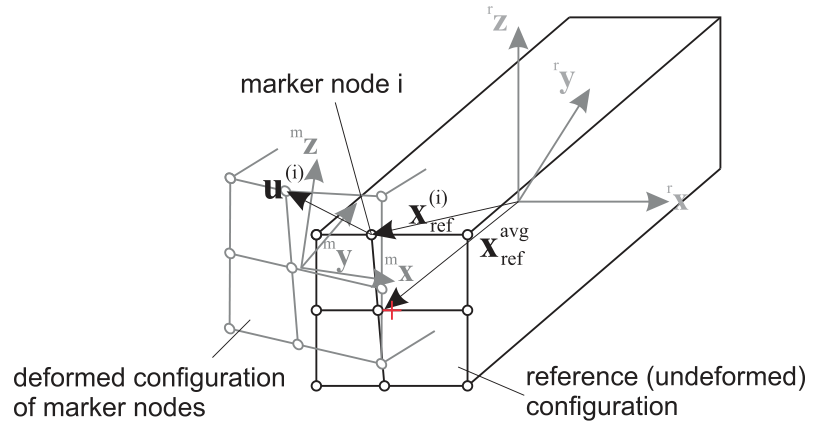
\includegraphics[width=10cm]{figures/MarkerSuperElementRigid.pdf}
      \end{center}
      \caption{Sketch of marker nodes, exemplary node $i$, reference coordinates and marker coordinate system; 
               note the difference of the center of the marker `surface' (rectangle) marked with the red cross, 
               and the averaged of the averaged local reference position.}
        \label{fig:MarkerSuperElementRigid:sketch}
    \end{figure}
    }
    \onlyRST{
    .. _fig-markersuperelementrigid-sketch:
    .. figure:: docs/theDoc/figures/MarkerSuperElementRigid.png
       :width: 400

       Sketch of marker nodes, exemplary node $i$, reference coordinates and marker coordinate system; note the difference of the center of the marker 'surface' (rectangle) marked with the red cross, and the averaged of the averaged local reference position.
    }
    %++++++++++++++++++++++++
    %++++++++++++++++++++++++++++++++++++++++++++++++++++++++++
    \mysubsubsubsection{Marker quantities}
    The marker provides a 'position' jacobian, which is the derivative of the global marker velocity w.r.t.\ the 
    object velocity coordinates $\dot \qv_{n_b}$,
    \be
      \LU{0}{\Jm_{m,pos}} = \frac{\partial \LU{0}{\vv}_{m}}{\dot \qv_{n_b}} \eqDot
    \ee
    In case of \texttt{ObjectGenericODE2}, assuming pure displacement based nodes,
    the jacobian will consist of zeros and unit matrices $\Im$ ,
    \be
      \LU{0}{\Jm_{m,pos}^{GenericODE2}} = \frac{\partial \LU{0}{\vv}_{m}}{\dot \qv_{n_b}} 
      = \left[ \Null,\; \ldots,\; \Null,\; w_0 \Im,\; \Null,\; \ldots,\; \Null,\; w_1 \Im,\; \Null,\; \ldots,\; \Null \right]\eqComma
    \ee
    in which the $\Im$ matrices are placed at the according indices of marker nodes.

    In case of \texttt{ObjectFFRFreducedOrder}, this jacobian is computed as weighted sum 
    of the position jacobians, see \texttt{ObjectFFRFreducedOrder},
    \be
      \LU{0}{\Jm_{m,pos}^{FFRFreduced}} = \frac{\partial \LU{0}{\vv}_{m}}{\dot \qv_{n_b}}
      = \sum_i w_i \LU{0}{\Jm^{(i)}_\mathrm{pos}}
      = \left[\Im, \; -\LU{0r}{\Rot} \left(\LU{r}{\ov\cRef} + \sum_i \LU{r}{\pv^{(i)}} \right) \LU{r}{\Gm},\;
              \sum_i w_i \LU{0r}{\Rot} \vr{\LU{r}{\tPsi_{r=3i}\tp}}{\LU{r}{\tPsi_{r=3i+1}\tp}}{\LU{r}{\tPsi_{r=3i+2}\tp}} \right] \eqDot
    \ee
    %\sum_i w_i \Im = \Im !!!
    %\be
    % \LU{0}{\Jm_\mathrm{pos}^{(i)}} = \frac{\partial \LU{0}{\pv^{(i)}}}{\partial [\qv\indt, \;\ttheta, \;\tzeta]}
    % = \left[\Im, \; -\LU{0b}{\Rot} \left(\LU{b}{\tilde\uv\indf^{(i)}} + \LU{b}{\tilde\xv^{(i)}\cRef} \right) \LU{b}{\Gm},\;
    %         \LU{0b}{\Rot} \vr{\LU{b}{\tPsi_{r=3i}\tp}}{\LU{b}{\tPsi_{r=3i+1}\tp}}{\LU{b}{\tPsi_{r=3i+2}\tp}}\right] \eqComma
    %\ee
    In \texttt{ObjectFFRFreducedOrder}, the jacobian usually affects all reduced coordinates.
    
    %++++++++++++++++++++++++++++++++++++++++++++
    \mysubsubsubsection{Standard approach for computation of rotation (\texttt{useAlternativeApproach = False})}
    %
    As compared to \texttt{MarkerSuperElementPosition}, \texttt{MarkerSuperElementRigid} also links the marker to the orientation of 
    the set of nodes provided. For this reason, the check performed in \texttt{mbs.assemble()} will take care that the nodes are capable
    to describe rotations.
    The first approach, here called as a standard, follows the idea that displacements contribute to rotation are weighted by their quadratic distance, 
    cf.\ \cite{HeirmanDesmet2010}, and gives the (small rotation) rotation vector
    \be
       \LU{r}{\ttheta}_{m} = \frac{\sum_i w_i \LU{r}{\pv_{ref}^{(i)}} \times \LU{r}{\uv^{(i)}}}{\sum_i w_i |\LU{r}{\pv_{ref}^{(i)}}|^2}
    \ee
    Note that $\pv_{ref}^{(i)}$ is not the reference position in the \texttt{ObjectFFRFreducedOrder} object, but it is relative to the midpoint reference position
    all marker nodes, given in $\LU{r}{\xv^\mathrm{avg}\cRef}$.
    %    
    Accordingly, the marker local angular velocity can be calculated as
    \be
       \LU{r}{\tomega}_{m} = \LU{r}{\dot \ttheta}_{m} = \frac{\sum_i w_i \LU{r}{\tilde \pv_{ref}^{(i)}} \LU{r}{\vv_i}}{\sum_i w_i |\LU{r}{\pv_{ref}^{(i)}}|^2}
    \ee
    %
    %++++++++++++++++++++++++++++++++++++++++++++++++++++++++++++++++++++++++++++++++++++++++++    
    The marker also provides a `rotation' jacobian, which is the derivative of the marker angular velocity $\LU{0}{\tomega}_{m}$ w.r.t.\ the 
    object velocity coordinates $\dot \qv_{n_b}$,
    \be
      \LU{0}{\Jm_{m,rot}} = \frac{\partial \LU{0}{\tomega}_{m}}{\partial \dot \qv_{n_b}}
                  = \frac{\partial \LU{0r}{\Rot}(\LU{r}{\tomega_{r}} + \LU{r}{\tomega}_{m})}{\partial \dot \qv_{n_b}}
                  = \LU{0r}{\Rot} \left(\frac{\partial \LU{r}{\tomega}_{r}}{\partial \dot \qv_{n_b}} + 
                                   \frac{\sum_i w_i \LU{r}{\tilde \pv_{ref}^{(i)}} \LU{r}{\Jm_{pos}^{(i)}}}{\sum_i w_i |\LU{r}{\pv_{ref}^{(i)}}|^2} \right)
    \ee
    In case of \texttt{ObjectFFRFreducedOrder}, this jacobian is computed as
    \be \label{eq:MarkerSuperElementRigid:jacRotStandard}
      \LU{0}{\Jm_{m,rot}^{FFRFreduced}} = \left[\Null,\; \LU{0r}{\Rot} \LU{r}{\Gm_{local}},\; 
                                                \LU{0r}{\Rot} \frac{\sum_i w_i \LU{r}{\tilde \pv_{ref}^{(i)}} \LU{r}{\Jm_{pos,f}^{(i)}}}{\sum_i w_i |\LU{r}{\pv_{ref}^{(i)}}|^2} \right]
    \ee
    in which you should know that
    \bi
      \item we used $\frac{\partial \LU{r}{\tomega_{r}} }{\partial \dot \ttheta_r} = \LU{r}{\Gm_{local}}$, 
      \item $\ttheta_{r}$ represent the rotation parameters for the rigid body node of \texttt{ObjectFFRFreducedOrder},
      \item $\LU{r}{\Jm_{pos,f}^{(i)}}$ is the {\bf local} jacobian, which only includes the flexible part of the local 
            jacobian for a single mesh node, $\LU{r}{\Jm_{pos}^{(i)}}$ (note the small $r$ on the upper left), 
            as defined in \texttt{ObjectFFRFreducedOrder}.
     \ei
    For further quantities also consult the according description in \texttt{ObjectFFRFreducedOrder}.
    \vspace{6pt}\\
    %
    %++++++++++++++++++++++++++++++++++++++++++++++++++++++++++++++++++++++++++++++++++++++++++    
    %++++++++++++++++++++++++++++++++++++++++++++++++++++++++++++++++++++++++++++++++++++++++++    
    \mysubsubsubsection{Alternative computation of rotation (\texttt{useAlternativeApproach = True})}
    Note that this approach is {\bf still under development} and needs further validation. 
    However, tests show that this model is superior to the standard approach, as it improves the averaging of motion w.r.t.\ rotations
    at the marker nodes.

    In the alternative approach, the weighting matrix $\Wm$ 
    has the interpretation of an inertia tensor built from nodes using weights equal to node masses.
    In such an interpretation, the 'local angular momentum' w.r.t.\ the marker (averaged) position can be computed as 
    \be \label{eq:MarkerSuperElementRigid:omegaAndWm}
       \Wm \LU{r}{\tomega}_{m} = \sum_i w_i \LU{r}{\tilde \pv_{ref}^{(i)}} \left(\LU{r}{\vv^{(i)}} - \LU{r}{\vv^\mathrm{avg}}\right)= 
       -\sum_i  \left( w_i \LU{r}{\tilde \pv_{ref}^{(i)}} \LU{r}{\tilde \pv_{ref}^{(i)}} \right) \LU{r}{\tomega}_{m}
    \ee
    which implicitly defines the weighting matrix $\Wm$, which must be invertable (but it is only a $3 \times 3$ matrix!),
    \be
        \Wm = -\sum_i  w_i \LU{r}{\tilde \pv_{ref}^{(i)}} \LU{r}{\tilde \pv_{ref}^{(i)}}
    \ee
    Furthermore, we need to introduce the averaged velocity of the marker averaged reference position, using $\LU{r}{\dot \uv^{(i)}} = \LU{r}{\vv^{(i)}}$, which is defined as
    \be
      \LU{r}{\vv^\mathrm{avg}} = \sum_i  w_i \LU{r}{\vv^{(i)}} \eqComma
    \ee
    similar to the averaged local reference position $\LU{r}{\xv^\mathrm{avg}\cRef}$ given in the table above, see also \fig{fig:MarkerSuperElementRigid:sketch}.

    In the alternative approach, thus the marker local rotations read
    \be
      \LU{r}{\ttheta}_{m,alt} = \Wm^{-1} \sum_i w_i \LU{r}{\tilde \pv_{ref}^{(i)}} \left( \LU{r}{\uv^{(i)}} - \LU{r}{\xv^\mathrm{avg}\cRef} \right) \eqComma
    \ee
    and the marker local angular velocity is defined as
    \be
      \LU{r}{\tomega}_{m,alt} = \Wm^{-1} \sum_i w_i \LU{r}{\tilde \pv_{ref}^{(i)}} \left( \LU{r}{\vv^{(i)}} - \LU{r}{\vv^\mathrm{avg}} \right) \eqDot
    \ee
    Note that, the average velocity $\LU{r}{\vv^\mathrm{avg}}$ would cancel out in a symmetric mesh, but would cause spurious 
    angular velocities in unsymmetric (w.r.t.\ the axis of rotation) distribition of mesh nodes. 
    This could even lead to spurious rotations or angular velocities in pure translatoric motion.

    %++++++++++++++++++++++++++++++++++++++++++++++++++++++++++++++++++++++++++++++++++++++++++    
    In the alternative mode, the Jacobian for the rotation / angular velocity is defined as
    \be
      \LU{0}{\Jm_{m,rot,alt}} = \frac{\partial \LU{0}{\tomega}_{m}}{\partial \dot \qv_{n_b}}
                  = \frac{\partial \LU{0r}{\Rot}(\LU{r}{\tomega_{r}} + \LU{r}{\tomega}_{m})}{\partial \dot \qv_{n_b}}
                  = \LU{0r}{\Rot} \left(\frac{\partial \LU{r}{\tomega}_{r}}{\partial \dot \qv_{n_b}}  + 
                                        \Wm^{-1} \sum_i w_i \LU{r}{\tilde \pv_{ref}^{(i)}} \LU{r}{\Jm_{pos}^{(i)}}\right)
    \ee
    In case of \texttt{ObjectFFRFreducedOrder}, this jacobian is computed as
    \be
      \LU{0}{\Jm_{m,rot,alt}^{FFRFreduced}} = \left[\Null,\; \LU{0r}{\Rot} \LU{r}{\Gm_{local}},\; 
                                                \LU{0r}{\Rot} \Wm^{-1} \sum_i w_i \LU{r}{\tilde \pv_{ref}^{(i)}} \LU{r}{\Jm_{pos,f}^{(i)}} \right]
    \ee
    see also the descriptions given after \eq{eq:MarkerSuperElementRigid:jacRotStandard} in the 'standard' approach.
    %
    \vspace{12pt}\\
    \noindent {\bf EXAMPLE for marker on body 4, mesh nodes 10,11,12,13}:\vspace{6pt}\\
    \texttt{MarkerSuperElementRigid(bodyNumber = 4, meshNodeNumber = [10, 11, 12, 13], weightingFactors = [0.25, 0.25, 0.25, 0.25], referencePosition=[0,0,0])}
    \vspace{12pt}\\
    \noindent For detailed examples, see \texttt{TestModels}.
    %%RSTCOMPATIBLE
\vspace{6pt}\par\noindent\rule{\textwidth}{0.4pt}
%
\noindent For examples on MarkerSuperElementRigid see Relevant Examples and TestModels with weblink:
\bi
\item \exuUrl{https://github.com/jgerstmayr/EXUDYN/blob/master/main/pythonDev/Examples/CMSexampleCourse.py}{\texttt{CMSexampleCourse.py}} (Examples/)
\item \exuUrl{https://github.com/jgerstmayr/EXUDYN/blob/master/main/pythonDev/Examples/netgenSTLtest.py}{\texttt{netgenSTLtest.py}} (Examples/)
\item \exuUrl{https://github.com/jgerstmayr/EXUDYN/blob/master/main/pythonDev/Examples/NGsolveCMStutorial.py}{\texttt{NGsolveCMStutorial.py}} (Examples/)
\item \exuUrl{https://github.com/jgerstmayr/EXUDYN/blob/master/main/pythonDev/Examples/NGsolveCraigBampton.py}{\texttt{NGsolveCraigBampton.py}} (Examples/)
\item \exuUrl{https://github.com/jgerstmayr/EXUDYN/blob/master/main/pythonDev/Examples/NGsolveLinearFEM.py}{\texttt{NGsolveLinearFEM.py}} (Examples/)
\item \exuUrl{https://github.com/jgerstmayr/EXUDYN/blob/master/main/pythonDev/Examples/ObjectFFRFconvergenceTestBeam.py}{\texttt{ObjectFFRFconvergenceTestBeam.py}} (Examples/)
\item \exuUrl{https://github.com/jgerstmayr/EXUDYN/blob/master/main/pythonDev/Examples/ObjectFFRFconvergenceTestHinge.py}{\texttt{ObjectFFRFconvergenceTestHinge.py}} (Examples/)
\item \exuUrl{https://github.com/jgerstmayr/EXUDYN/blob/master/main/pythonDev/Examples/pendulumVerify.py}{\texttt{pendulumVerify.py}} (Examples/)
\item \exuUrl{https://github.com/jgerstmayr/EXUDYN/blob/master/main/pythonDev/Examples/serialRobotFlexible.py}{\texttt{serialRobotFlexible.py}} (Examples/)
\item \exuUrl{https://github.com/jgerstmayr/EXUDYN/blob/master/main/pythonDev/TestModels/abaqusImportTest.py}{\texttt{abaqusImportTest.py}} (TestModels/)
\item \exuUrl{https://github.com/jgerstmayr/EXUDYN/blob/master/main/pythonDev/TestModels/ACFtest.py}{\texttt{ACFtest.py}} (TestModels/)
\item \exuUrl{https://github.com/jgerstmayr/EXUDYN/blob/master/main/pythonDev/TestModels/superElementRigidJointTest.py}{\texttt{superElementRigidJointTest.py}} (TestModels/)

\ei

%
\newpage

%+++++++++++++++++++++++++++++++++++

\mysubsubsection{MarkerKinematicTreeRigid}
\label{sec:item:MarkerKinematicTreeRigid}
A position and orientation (rigid-body) marker attached to a kinematic tree. The marker is attached to the ObjectKinematicTree object and additionally needs a link number as well as a local position, similar to the SensorKinematicTree. The marker allows to attach loads (LoadForceVector and LoadTorqueVector) at arbitrary links or position. It also allows to attach connectors (e.g., spring dampers or actuators) to the kinematic tree. Finally, joint constraints can be attached, which allows for realization of closed loop structures. NOTE, however, that it is less efficient to attach many markers to a kinematic tree, therefor for forces or joint control use the structures available in kinematic tree whenever possible.
\vspace{12pt}\\

\noindent \mybold{Additional information for MarkerKinematicTreeRigid}:
\bi
  \item This \texttt{Marker} has/provides the following types = \texttt{Object}, \texttt{Body}, \texttt{Position}, \texttt{Orientation}
\ei\vspace{12pt} \noindent 
The item \mybold{MarkerKinematicTreeRigid} with type = 'KinematicTreeRigid' has the following parameters:
\vspace{-0.5cm}\\
\vspace{-0.5cm}\\
%reference manual TABLE
\begin{center}
  \footnotesize
  \begin{longtable}{| p{4.5cm} | p{2.5cm} | p{0.5cm} | p{2.5cm} | p{6cm} |}
    \hline
    \bf Name & \bf type & \bf size & \bf default value & \bf description \\ \hline
    name &     String &      &     '' &     marker's unique name\\ \hline
    objectNumber &     ObjectIndex &      &     invalid (-1) &     \tabnewline body number to which marker is attached to\\ \hline
    linkNumber &     UInt &      &     invalid (-1) &     \tabnewline number of link in KinematicTree to which marker is attached to\\ \hline
    localPosition &     Vector3D &     3 &     [0.,0.,0.] &     \tabnewline local (link-fixed) position of marker at link $n_l$, using the link ($n_l$) coordinate system\\ \hline
    visualization &     VMarkerKinematicTreeRigid &      &      &     parameters for visualization of item\\ \hline
\end{longtable}
\end{center}

\noindent The item VMarkerKinematicTreeRigid has the following parameters:
%reference manual TABLE
\begin{center}
  \footnotesize
  \begin{longtable}{| p{4.5cm} | p{2.5cm} | p{0.5cm} | p{2.5cm} | p{6cm} |}
    \hline
    \bf Name & \bf type & \bf size & \bf default value & \bf description \\ \hline
    show &     Bool &      &     True &     set true, if item is shown in visualization and false if it is not shown\\ \hline
\end{longtable}
\end{center}
\par\noindent\rule{\textwidth}{0.4pt}
\mysubsubsubsection{DESCRIPTION of MarkerKinematicTreeRigid:}
\label{description_MarkerKinematicTreeRigid}
\paragraph{Information on input parameters:} 
\startTable{input parameter}{symbol}{description see tables above}
\rowTable{objectNumber}{$n_b$}{}
\rowTable{linkNumber}{$n_l$}{}
\rowTable{localPosition}{$\LU{l}{\bv}$}{}
\finishTable
 \noindent
    %    {\bf Definition of marker quantities}:
    %    \startTable{intermediate variables}{symbol}{description}
    %    \rowTable{marker position}{$\LU{0}{\pv}_{m} \!=\! \LU{0}{\pv}_r + \LU{0r}{\Rot} \left(\LU{r}{\ov\cRef}\! +\! \sum_i w_i \cdot \LU{r}{\pv^{(i)}} \right)$}
    %             {current global position which is provided by marker; note offset $\LU{r}{\ov\cRef}$ added, if used as a correction of marker mesh nodes}
    %    \rowTable{marker velocity}{$\LU{0}{\vv}_{m} = \LU{0}{\dot \pv}_r + \LU{0r}{\Rot} \left( \LU{r}{\tilde \tomega_r} \sum_i (w_i \cdot \LU{r}{\pv^{(i)}}) + \right.
    %             \left. \sum_i (w_i \cdot \LU{r}{\dot \uv^{(i)}}) \right)$}
    %             {current global velocity which is provided by marker}
    %    \rowTable{marker rotation matrix}{$\LU{0r}{\Rot}_{m} = \LU{0r}{\Rot} \cdot \mathbf{exp}(\LU{r}{\ttheta}_{m})$}{current rotation matrix, which transforms the local marker coordinates and adds the rigid body transformation of floating frames $\LU{0r}{\Rot}$; uses exponential map for SO3, assumes that $\ttheta$ represents a rotation vector}
    %    \rowTable{marker local rotation}{$\LU{r}{\ttheta}_{m}$}{current local linearized rotations (rotation vector); for the computation, see below for the standard and alternative approach}
    %    
    %    \rowTable{marker local angular velocity}{$\LU{r}{\tomega}_{m}$}{local angular velocity due to mesh node velocity only; for the computation, see below for the standard and alternative approach}
    %    \rowTable{marker global angular velocity}{$\LU{0}{\tomega}_{m} = \LU{0}{\tomega_{r}} + \LU{0r}{\Rot} \LU{r}{\tomega}_{m}$}{current global angular velocity}
    %    \finishTable
    %
    %    \vspace{6pt}
    %++++++++++++++++++++++++++++++++++++++++++++++++++++++++++
    \mysubsubsubsection{Marker quantities}
    More information will be added later. The marker computes jacobians according to \texttt{Jacobian} in \texttt{class Robot}.
    %%RSTCOMPATIBLE
    %    The marker provides a 'position' jacobian, which is the derivative of the global marker velocity w.r.t.\ the 
    %    object velocity coordinates $\dot \qv_{n_b}$,
    %    \be
    %      \LU{0}{\Jm_{m,pos}} = \frac{\partial \LU{0}{\vv}_{m}}{\dot \qv_{n_b}} \eqDot
    %    \ee
    %    In case of \texttt{ObjectGenericODE2}, assuming pure displacement based nodes,
    %    the jacobian will consist of zeros and unit matrices $\Im$ ,
    %    \be
    %      \LU{0}{\Jm_{m,pos}^{GenericODE2}} = \frac{\partial \LU{0}{\vv}_{m}}{\dot \qv_{n_b}} 
    %      = \left[ \Null,\; \ldots,\; \Null,\; \Im,\; \Null,\; \ldots,\; \Null,\; \Im,\; \Null,\; \ldots,\; \Null \right]\eqComma
    %    \ee
    %    in which the $\Im$ matrices are placed at the according indices of marker nodes.
    %    In case of \texttt{ObjectFFRFreducedOrder}, this jacobian is computed as weighted sum 
    %    of the position jacobians, see \texttt{ObjectFFRFreducedOrder},
    %    \be
    %      \LU{0}{\Jm_{m,pos}^{FFRFreduced}} = \frac{\partial \LU{0}{\vv}_{m}}{\dot \qv_{n_b}}
    %      = \sum_i w_i \LU{0}{\Jm^{(i)}_\mathrm{pos}}
    %      = \left[\Im, \; -\LU{0r}{\Rot} \left(\sum_i(\LU{r}{\tilde\uv\indf^{(i)}} + \LU{r}{\tilde\xv^{(i)}\cRef}) \right) \LU{r}{\Gm},\;
    %              \sum_i w_i \LU{0r}{\Rot} \vr{\LU{r}{\tPsi_{r=3i}\tp}}{\LU{r}{\tPsi_{r=3i+1}\tp}}{\LU{r}{\tPsi_{r=3i+2}\tp}} \right] \eqDot
    %    \ee
    %    In \texttt{ObjectFFRFreducedOrder}, the jacobian usually affects all reduced coordinates.
    %
\vspace{6pt}\par\noindent\rule{\textwidth}{0.4pt}
%
\noindent For examples on MarkerKinematicTreeRigid see Relevant Examples and TestModels with weblink:
\bi
\item \exuUrl{https://github.com/jgerstmayr/EXUDYN/blob/master/main/pythonDev/Examples/humanRobotInteraction.py}{\texttt{humanRobotInteraction.py}} (Examples/)
\item \exuUrl{https://github.com/jgerstmayr/EXUDYN/blob/master/main/pythonDev/Examples/reinforcementLearningRobot.py}{\texttt{reinforcementLearningRobot.py}} (Examples/)
\item \exuUrl{https://github.com/jgerstmayr/EXUDYN/blob/master/main/pythonDev/Examples/serialRobotKinematicTreeDigging.py}{\texttt{serialRobotKinematicTreeDigging.py}} (Examples/)
\item \exuUrl{https://github.com/jgerstmayr/EXUDYN/blob/master/main/pythonDev/Examples/stiffFlyballGovernorKT.py}{\texttt{stiffFlyballGovernorKT.py}} (Examples/)
\item \exuUrl{https://github.com/jgerstmayr/EXUDYN/blob/master/main/pythonDev/TestModels/kinematicTreeConstraintTest.py}{\texttt{kinematicTreeConstraintTest.py}} (TestModels/)

\ei

%
\newpage

%+++++++++++++++++++++++++++++++++++

\mysubsubsection{MarkerObjectODE2Coordinates}
\label{sec:item:MarkerObjectODE2Coordinates}
A Marker attached to all coordinates of an object (currently only body is possible), e.g. to apply special constraints or loads on all coordinates. The measured coordinates INCLUDE reference + current coordinates.
\vspace{12pt}\\

\noindent \mybold{Additional information for MarkerObjectODE2Coordinates}:
\bi
  \item This \texttt{Marker} has/provides the following types = \texttt{Object}, \texttt{Body}, \texttt{Coordinate}
\ei\vspace{12pt} \noindent 
The item \mybold{MarkerObjectODE2Coordinates} with type = 'ObjectODE2Coordinates' has the following parameters:
\vspace{-0.5cm}\\
\vspace{-0.5cm}\\
%reference manual TABLE
\begin{center}
  \footnotesize
  \begin{longtable}{| p{4.5cm} | p{2.5cm} | p{0.5cm} | p{2.5cm} | p{6cm} |}
    \hline
    \bf Name & \bf type & \bf size & \bf default value & \bf description \\ \hline
    name &     String &      &     '' &     marker's unique name\\ \hline
    objectNumber &     ObjectIndex &      &     invalid (-1) &     \tabnewline body number to which marker is attached to\\ \hline
    visualization &     VMarkerObjectODE2Coordinates &      &      &     parameters for visualization of item\\ \hline
\end{longtable}
\end{center}

\noindent The item VMarkerObjectODE2Coordinates has the following parameters:
%reference manual TABLE
\begin{center}
  \footnotesize
  \begin{longtable}{| p{4.5cm} | p{2.5cm} | p{0.5cm} | p{2.5cm} | p{6cm} |}
    \hline
    \bf Name & \bf type & \bf size & \bf default value & \bf description \\ \hline
    show &     Bool &      &     True &     set true, if item is shown in visualization and false if it is not shown\\ \hline
\end{longtable}
\end{center}
\par\noindent\rule{\textwidth}{0.4pt}
\mysubsubsubsection{DESCRIPTION of MarkerObjectODE2Coordinates:}
\label{description_MarkerObjectODE2Coordinates}
\vspace{6pt}\par\noindent\rule{\textwidth}{0.4pt}
%
\noindent For examples on MarkerObjectODE2Coordinates see Relevant Examples and TestModels with weblink:
\bi
\item \exuUrl{https://github.com/jgerstmayr/EXUDYN/blob/master/main/pythonDev/TestModels/coordinateVectorConstraintGenericODE2.py}{\texttt{coordinateVectorConstraintGenericODE2.py}} (TestModels/)

\ei

%
\newpage

%+++++++++++++++++++++++++++++++++++

\mysubsubsection{MarkerBodyCable2DShape}
\label{sec:item:MarkerBodyCable2DShape}
A special Marker attached to a 2D ANCF beam finite element with cubic interpolation and 8 coordinates.
\vspace{12pt}\\

\noindent \mybold{Additional information for MarkerBodyCable2DShape}:
\bi
  \item This \texttt{Marker} has/provides the following types = \texttt{Object}, \texttt{Body}, \texttt{Coordinate}
\ei\vspace{12pt} \noindent 
The item \mybold{MarkerBodyCable2DShape} with type = 'BodyCable2DShape' has the following parameters:
\vspace{-0.5cm}\\
\vspace{-0.5cm}\\
%reference manual TABLE
\begin{center}
  \footnotesize
  \begin{longtable}{| p{4.5cm} | p{2.5cm} | p{0.5cm} | p{2.5cm} | p{6cm} |}
    \hline
    \bf Name & \bf type & \bf size & \bf default value & \bf description \\ \hline
    name &     String &      &     '' &     marker's unique name\\ \hline
    bodyNumber &     ObjectIndex &      &     invalid (-1) &     \tabnewline body number to which marker is attached to\\ \hline
    numberOfSegments &     PInt &      &     3 &     number of number of segments; each segment is a line and is associated to a data (history) variable; must be same as in according contact element\\ \hline
    verticalOffset &     Real &      &     0. &     vertical offset from beam axis in positive (local) Y-direction; this offset accounts for consistent computation of positions and velocities at the surface of the beam\\ \hline
    visualization &     VMarkerBodyCable2DShape &      &      &     parameters for visualization of item\\ \hline
\end{longtable}
\end{center}

\noindent The item VMarkerBodyCable2DShape has the following parameters:
%reference manual TABLE
\begin{center}
  \footnotesize
  \begin{longtable}{| p{4.5cm} | p{2.5cm} | p{0.5cm} | p{2.5cm} | p{6cm} |}
    \hline
    \bf Name & \bf type & \bf size & \bf default value & \bf description \\ \hline
    show &     Bool &      &     True &     set true, if item is shown in visualization and false if it is not shown\\ \hline
\end{longtable}
\end{center}
\par\noindent\rule{\textwidth}{0.4pt}
\mysubsubsubsection{DESCRIPTION of MarkerBodyCable2DShape:}
\label{description_MarkerBodyCable2DShape}
\vspace{6pt}\par\noindent\rule{\textwidth}{0.4pt}
%
\noindent For examples on MarkerBodyCable2DShape see Relevant Examples and TestModels with weblink:
\bi
\item \exuUrl{https://github.com/jgerstmayr/EXUDYN/blob/master/main/pythonDev/Examples/ANCFcontactCircle.py}{\texttt{ANCFcontactCircle.py}} (Examples/)
\item \exuUrl{https://github.com/jgerstmayr/EXUDYN/blob/master/main/pythonDev/Examples/ANCFcontactCircle2.py}{\texttt{ANCFcontactCircle2.py}} (Examples/)
\item \exuUrl{https://github.com/jgerstmayr/EXUDYN/blob/master/main/pythonDev/Examples/ANCFmovingRigidbody.py}{\texttt{ANCFmovingRigidbody.py}} (Examples/)
\item \exuUrl{https://github.com/jgerstmayr/EXUDYN/blob/master/main/pythonDev/Examples/ANCFslidingJoint2D.py}{\texttt{ANCFslidingJoint2D.py}} (Examples/)
\item \exuUrl{https://github.com/jgerstmayr/EXUDYN/blob/master/main/pythonDev/Examples/beltDriveALE.py}{\texttt{beltDriveALE.py}} (Examples/)
\item \exuUrl{https://github.com/jgerstmayr/EXUDYN/blob/master/main/pythonDev/Examples/beltDriveReevingSystem.py}{\texttt{beltDriveReevingSystem.py}} (Examples/)
\item \exuUrl{https://github.com/jgerstmayr/EXUDYN/blob/master/main/pythonDev/Examples/beltDrivesComparison.py}{\texttt{beltDrivesComparison.py}} (Examples/)
\item \exuUrl{https://github.com/jgerstmayr/EXUDYN/blob/master/main/pythonDev/Examples/sliderCrank3DwithANCFbeltDrive.py}{\texttt{sliderCrank3DwithANCFbeltDrive.py}} (Examples/)
\item \exuUrl{https://github.com/jgerstmayr/EXUDYN/blob/master/main/pythonDev/Examples/sliderCrank3DwithANCFbeltDrive2.py}{\texttt{sliderCrank3DwithANCFbeltDrive2.py}} (Examples/)
\item \exuUrl{https://github.com/jgerstmayr/EXUDYN/blob/master/main/pythonDev/TestModels/ANCFcontactCircleTest.py}{\texttt{ANCFcontactCircleTest.py}} (TestModels/)
\item \exuUrl{https://github.com/jgerstmayr/EXUDYN/blob/master/main/pythonDev/TestModels/ANCFcontactFrictionTest.py}{\texttt{ANCFcontactFrictionTest.py}} (TestModels/)
\item \exuUrl{https://github.com/jgerstmayr/EXUDYN/blob/master/main/pythonDev/TestModels/ANCFmovingRigidBodyTest.py}{\texttt{ANCFmovingRigidBodyTest.py}} (TestModels/)
\item \exuUrl{https://github.com/jgerstmayr/EXUDYN/blob/master/main/pythonDev/TestModels/ANCFslidingAndALEjointTest.py}{\texttt{ANCFslidingAndALEjointTest.py}} (TestModels/)

\ei

%
\newpage

%+++++++++++++++++++++++++++++++++++

\mysubsubsection{MarkerBodyCable2DCoordinates}
\label{sec:item:MarkerBodyCable2DCoordinates}
A special Marker attached to the coordinates of a 2D ANCF beam finite element with cubic interpolation.
\vspace{12pt}\\

\noindent \mybold{Additional information for MarkerBodyCable2DCoordinates}:
\bi
  \item This \texttt{Marker} has/provides the following types = \texttt{Object}, \texttt{Body}, \texttt{Coordinate}
\ei\vspace{12pt} \noindent 
The item \mybold{MarkerBodyCable2DCoordinates} with type = 'BodyCable2DCoordinates' has the following parameters:
\vspace{-0.5cm}\\
\vspace{-0.5cm}\\
%reference manual TABLE
\begin{center}
  \footnotesize
  \begin{longtable}{| p{4.5cm} | p{2.5cm} | p{0.5cm} | p{2.5cm} | p{6cm} |}
    \hline
    \bf Name & \bf type & \bf size & \bf default value & \bf description \\ \hline
    name &     String &      &     '' &     marker's unique name\\ \hline
    bodyNumber &     ObjectIndex &      &     invalid (-1) &     \tabnewline body number to which marker is attached to\\ \hline
    visualization &     VMarkerBodyCable2DCoordinates &      &      &     parameters for visualization of item\\ \hline
\end{longtable}
\end{center}

\noindent The item VMarkerBodyCable2DCoordinates has the following parameters:
%reference manual TABLE
\begin{center}
  \footnotesize
  \begin{longtable}{| p{4.5cm} | p{2.5cm} | p{0.5cm} | p{2.5cm} | p{6cm} |}
    \hline
    \bf Name & \bf type & \bf size & \bf default value & \bf description \\ \hline
    show &     Bool &      &     True &     set true, if item is shown in visualization and false if it is not shown\\ \hline
\end{longtable}
\end{center}
\par\noindent\rule{\textwidth}{0.4pt}
\mysubsubsubsection{DESCRIPTION of MarkerBodyCable2DCoordinates:}
\label{description_MarkerBodyCable2DCoordinates}
\vspace{6pt}\par\noindent\rule{\textwidth}{0.4pt}
%
\noindent For examples on MarkerBodyCable2DCoordinates see Relevant Examples and TestModels with weblink:
\bi
\item \exuUrl{https://github.com/jgerstmayr/EXUDYN/blob/master/main/pythonDev/Examples/ANCFmovingRigidbody.py}{\texttt{ANCFmovingRigidbody.py}} (Examples/)
\item \exuUrl{https://github.com/jgerstmayr/EXUDYN/blob/master/main/pythonDev/Examples/ANCFslidingJoint2D.py}{\texttt{ANCFslidingJoint2D.py}} (Examples/)
\item \exuUrl{https://github.com/jgerstmayr/EXUDYN/blob/master/main/pythonDev/Examples/ANCFslidingJoint2Drigid.py}{\texttt{ANCFslidingJoint2Drigid.py}} (Examples/)
\item \exuUrl{https://github.com/jgerstmayr/EXUDYN/blob/master/main/pythonDev/Examples/ANCFswitchingSlidingJoint2D.py}{\texttt{ANCFswitchingSlidingJoint2D.py}} (Examples/)
\item \exuUrl{https://github.com/jgerstmayr/EXUDYN/blob/master/main/pythonDev/TestModels/ANCFmovingRigidBodyTest.py}{\texttt{ANCFmovingRigidBodyTest.py}} (TestModels/)
\item \exuUrl{https://github.com/jgerstmayr/EXUDYN/blob/master/main/pythonDev/TestModels/modelUnitTests.py}{\texttt{modelUnitTests.py}} (TestModels/)

\ei

%

\newpage
%+++++++++++++++++++++++++++++++
%+++++++++++++++++++++++++++++++
\mysubsection{Loads}
A Load applies a (usually constant) force, torque, mass-proportional or generalized load onto Nodes or Objects via Markers. The requested \texttt{Marker} types need to be provided by the used \text{Marker}. The marker may provide more types than requested. For non-constant loads, use either a \texttt{load...UserFunction} or change the load in every step by means of a \texttt{preStepUserFunction} in the \texttt{MainSystem} (mbs).
%++++++

%+++++++++++++++++++++++++++++++++++

\mysubsubsection{LoadForceVector}
\label{sec:item:LoadForceVector}
Load with (3D) force vector; attached to position-based marker.
\vspace{12pt}\\

\noindent \mybold{Additional information for LoadForceVector}:
\bi
  \item Requested \texttt{Marker} type = \texttt{Position}
  \item {\bf Short name} for Python = \texttt{Force}
  \item {\bf Short name} for Python visualization object = \texttt{VForce}
\ei\vspace{12pt} \noindent 
The item \mybold{LoadForceVector} with type = 'ForceVector' has the following parameters:
\vspace{-0.5cm}\\
\vspace{-0.5cm}\\
%reference manual TABLE
\begin{center}
  \footnotesize
  \begin{longtable}{| p{4.5cm} | p{2.5cm} | p{0.5cm} | p{2.5cm} | p{6cm} |}
    \hline
    \bf Name & \bf type & \bf size & \bf default value & \bf description \\ \hline
    name &     String &      &     '' &     load's unique name\\ \hline
    markerNumber &     MarkerIndex &      &     invalid (-1) &     \tabnewline marker's number to which load is applied\\ \hline
    loadVector &     Vector3D &      &     [0.,0.,0.] &     \tabnewline vector-valued load [SI:N]; in case of a user function, this vector is ignored\\ \hline
    bodyFixed &     Bool &      &     False &     if bodyFixed is true, the load is defined in body-fixed (local) coordinates, leading to a follower force; if false: global coordinates are used\\ \hline
    loadVectorUserFunction &     PyFunctionVector3DmbsScalarVector3D &     \tabnewline  &     \tabnewline 0 &     A Python function which defines the time-dependent load and replaces loadVector; see description below; NOTE that in static computations, the loadFactor is always 1 for forces computed by user functions (this means for the static computation, that a user function returning [t*5,t*1,0] corresponds to loadVector=[5,1,0] without a user function); NOTE that forces are drawn using the value of loadVector; thus the current values according to the user function are NOT shown in the render window; however, a sensor (SensorLoad) returns the user function force which is applied to the object; to draw forces with current user function values, use a graphicsDataUserFunction of a ground object\\ \hline
    visualization &     VLoadForceVector &      &      &     parameters for visualization of item\\ \hline
\end{longtable}
\end{center}

\noindent The item VLoadForceVector has the following parameters:
%reference manual TABLE
\begin{center}
  \footnotesize
  \begin{longtable}{| p{4.5cm} | p{2.5cm} | p{0.5cm} | p{2.5cm} | p{6cm} |}
    \hline
    \bf Name & \bf type & \bf size & \bf default value & \bf description \\ \hline
    show &     Bool &      &     True &     set true, if item is shown in visualization and false if it is not shown\\ \hline
\end{longtable}
\end{center}
\par\noindent\rule{\textwidth}{0.4pt}
\mysubsubsubsection{DESCRIPTION of LoadForceVector:}
\label{description_LoadForceVector}
\paragraph{Information on input parameters:} 
\startTable{input parameter}{symbol}{description see tables above}
\rowTable{loadVector}{$\fv$}{}
\rowTable{loadVectorUserFunction}{$\mathrm{UF} \in \Rcal^3$}{}
\finishTable
 \noindent
    \mysubsubsubsection{Details}
    The load vector acts on a body or node via the local (\texttt{bodyFixed = True}) or global coordinates of a body or at a node. 
    The marker transforms the (translational) force via the according jacobian matrix of the object (or node) to object (or node) coordinates.
    %
    %++++++++++++++++++++++++++++++++++++++++++++++++++++++++++
    \userFunction{loadVectorUserFunction(mbs, t, loadVector)}
    A user function, which computes the force vector depending on time and object parameters, which is hereafter applied to object or node.
    %
    \startTable{arguments / return}{type or size}{description}
      \rowTable{\texttt{mbs}}{MainSystem}{provides MainSystem mbs to which load belongs}
      \rowTable{\texttt{t}}{Real}{current time in mbs} %use t instead time in order to avoid possible conflicts with Python time
      \rowTable{\texttt{loadVector}}{Vector3D}{$\fv$ copied from object; WARNING: this parameter does not work in combination with static computation, as it is changed by the solver over step time}
      \rowTable{\returnValue}{Vector3D}{computed force vector}
    \finishTable
    %++++++++++++++++++++++++++++++++++++++++++++++++++++++++++
    \userFunctionExample{}
    \pythonstyle\begin{lstlisting}
        from math import sin, cos, pi
        def UFforce(mbs, t, loadVector): 
            return [loadVector[0]*sin(t*10*2*pi),0,0]
    \end{lstlisting}
    %%RSTCOMPATIBLE
\vspace{6pt}\par\noindent\rule{\textwidth}{0.4pt}
%
\noindent For examples on LoadForceVector see Relevant Examples and TestModels with weblink:
\bi
\item \exuUrl{https://github.com/jgerstmayr/EXUDYN/blob/master/main/pythonDev/Examples/interactiveTutorial.py}{\texttt{interactiveTutorial.py}} (Examples/)
\item \exuUrl{https://github.com/jgerstmayr/EXUDYN/blob/master/main/pythonDev/Examples/pendulumVerify.py}{\texttt{pendulumVerify.py}} (Examples/)
\item \exuUrl{https://github.com/jgerstmayr/EXUDYN/blob/master/main/pythonDev/Examples/ROSMassPoint.py}{\texttt{ROSMassPoint.py}} (Examples/)
\item \exuUrl{https://github.com/jgerstmayr/EXUDYN/blob/master/main/pythonDev/Examples/solutionViewerTest.py}{\texttt{solutionViewerTest.py}} (Examples/)
\item \exuUrl{https://github.com/jgerstmayr/EXUDYN/blob/master/main/pythonDev/Examples/SpringDamperMassUserFunction.py}{\texttt{SpringDamperMassUserFunction.py}} (Examples/)
\item \exuUrl{https://github.com/jgerstmayr/EXUDYN/blob/master/main/pythonDev/Examples/ANCFcantileverTest.py}{\texttt{ANCFcantileverTest.py}} (Examples/)
\item \exuUrl{https://github.com/jgerstmayr/EXUDYN/blob/master/main/pythonDev/Examples/ANCFcantileverTestDyn.py}{\texttt{ANCFcantileverTestDyn.py}} (Examples/)
\item \exuUrl{https://github.com/jgerstmayr/EXUDYN/blob/master/main/pythonDev/Examples/ANCFcontactCircle.py}{\texttt{ANCFcontactCircle.py}} (Examples/)
\item \exuUrl{https://github.com/jgerstmayr/EXUDYN/blob/master/main/pythonDev/Examples/ANCFcontactCircle2.py}{\texttt{ANCFcontactCircle2.py}} (Examples/)
\item \exuUrl{https://github.com/jgerstmayr/EXUDYN/blob/master/main/pythonDev/Examples/ANCFmovingRigidbody.py}{\texttt{ANCFmovingRigidbody.py}} (Examples/)
\item \exuUrl{https://github.com/jgerstmayr/EXUDYN/blob/master/main/pythonDev/Examples/ANCFrotatingCable2D.py}{\texttt{ANCFrotatingCable2D.py}} (Examples/)
\item \exuUrl{https://github.com/jgerstmayr/EXUDYN/blob/master/main/pythonDev/Examples/ANCFslidingJoint2D.py}{\texttt{ANCFslidingJoint2D.py}} (Examples/)
\item  ...

\item \exuUrl{https://github.com/jgerstmayr/EXUDYN/blob/master/main/pythonDev/TestModels/perf3DRigidBodies.py}{\texttt{perf3DRigidBodies.py}} (TestModels/)
\item \exuUrl{https://github.com/jgerstmayr/EXUDYN/blob/master/main/pythonDev/TestModels/plotSensorTest.py}{\texttt{plotSensorTest.py}} (TestModels/)
\item \exuUrl{https://github.com/jgerstmayr/EXUDYN/blob/master/main/pythonDev/TestModels/revoluteJointPrismaticJointTest.py}{\texttt{revoluteJointPrismaticJointTest.py}} (TestModels/)
\item  ...


\ei

%
\newpage

%+++++++++++++++++++++++++++++++++++

\mysubsubsection{LoadTorqueVector}
\label{sec:item:LoadTorqueVector}
Load with (3D) torque vector; attached to rigidbody-based marker.
\vspace{12pt}\\

\noindent \mybold{Additional information for LoadTorqueVector}:
\bi
  \item Requested \texttt{Marker} type = \texttt{Orientation}
  \item {\bf Short name} for Python = \texttt{Torque}
  \item {\bf Short name} for Python visualization object = \texttt{VTorque}
\ei\vspace{12pt} \noindent 
The item \mybold{LoadTorqueVector} with type = 'TorqueVector' has the following parameters:
\vspace{-0.5cm}\\
\vspace{-0.5cm}\\
%reference manual TABLE
\begin{center}
  \footnotesize
  \begin{longtable}{| p{4.5cm} | p{2.5cm} | p{0.5cm} | p{2.5cm} | p{6cm} |}
    \hline
    \bf Name & \bf type & \bf size & \bf default value & \bf description \\ \hline
    name &     String &      &     '' &     load's unique name\\ \hline
    markerNumber &     MarkerIndex &      &     invalid (-1) &     \tabnewline marker's number to which load is applied\\ \hline
    loadVector &     Vector3D &      &     [0.,0.,0.] &     \tabnewline vector-valued load [SI:N]; in case of a user function, this vector is ignored\\ \hline
    bodyFixed &     Bool &      &     False &     if bodyFixed is true, the load is defined in body-fixed (local) coordinates, leading to a follower torque; if false: global coordinates are used\\ \hline
    loadVectorUserFunction &     PyFunctionVector3DmbsScalarVector3D &     \tabnewline  &     \tabnewline 0 &     A Python function which defines the time-dependent load and replaces loadVector; see description below; see also notes on loadFactor and drawing in LoadForceVector! Example for Python function: def f(mbs, t, loadVector): return [loadVector[0]*np.sin(t*10*2*3.1415),0,0]\\ \hline
    visualization &     VLoadTorqueVector &      &      &     parameters for visualization of item\\ \hline
\end{longtable}
\end{center}

\noindent The item VLoadTorqueVector has the following parameters:
%reference manual TABLE
\begin{center}
  \footnotesize
  \begin{longtable}{| p{4.5cm} | p{2.5cm} | p{0.5cm} | p{2.5cm} | p{6cm} |}
    \hline
    \bf Name & \bf type & \bf size & \bf default value & \bf description \\ \hline
    show &     Bool &      &     True &     set true, if item is shown in visualization and false if it is not shown\\ \hline
\end{longtable}
\end{center}
\par\noindent\rule{\textwidth}{0.4pt}
\mysubsubsubsection{DESCRIPTION of LoadTorqueVector:}
\label{description_LoadTorqueVector}
\paragraph{Information on input parameters:} 
\startTable{input parameter}{symbol}{description see tables above}
\rowTable{loadVector}{$\ttau$}{}
\rowTable{loadVectorUserFunction}{$\mathrm{UF} \in \Rcal^3$}{}
\finishTable
 \noindent
    \mysubsubsubsection{Details}
    The torque vector acts on a body or node via the local (\texttt{bodyFixed = True}) or global coordinates of a body or at a node. 
    The marker transforms the torque via the according jacobian matrix of the object (or node) to object (or node) coordinates.
    %
    %++++++++++++++++++++++++++++++++++++++++++++++++++++++++++
    \userFunction{loadVectorUserFunction(mbs, t, loadVector)}
    A user function, which computes the torque vector depending on time and object parameters, which is hereafter applied to object or node.
    %
    \startTable{arguments / return}{type or size}{description}
      \rowTable{\texttt{mbs}}{MainSystem}{provides MainSystem mbs to which load belongs}
      \rowTable{\texttt{t}}{Real}{current time in mbs} %use t instead time in order to avoid possible conflicts with Python time
      \rowTable{\texttt{loadVector}}{Vector3D}{$\ttau$ copied from object; WARNING: this parameter does not work in combination with static computation, as it is changed by the solver over step time}
      \rowTable{\returnValue}{Vector3D}{computed torque vector}
    \finishTable
    %++++++++++++++++++++++++++++++++++++++++++++++++++++++++++
    \userFunctionExample{}
    \pythonstyle\begin{lstlisting}
        from math import sin, cos, pi
        def UFforce(mbs, t, loadVector): 
            return [loadVector[0]*sin(t*10*2*pi),0,0]
    \end{lstlisting}
    %%RSTCOMPATIBLE
\vspace{6pt}\par\noindent\rule{\textwidth}{0.4pt}
%
\noindent For examples on LoadTorqueVector see Relevant Examples and TestModels with weblink:
\bi
\item \exuUrl{https://github.com/jgerstmayr/EXUDYN/blob/master/main/pythonDev/Examples/leggedRobot.py}{\texttt{leggedRobot.py}} (Examples/)
\item \exuUrl{https://github.com/jgerstmayr/EXUDYN/blob/master/main/pythonDev/Examples/reevingSystem.py}{\texttt{reevingSystem.py}} (Examples/)
\item \exuUrl{https://github.com/jgerstmayr/EXUDYN/blob/master/main/pythonDev/Examples/sliderCrank3DwithANCFbeltDrive2.py}{\texttt{sliderCrank3DwithANCFbeltDrive2.py}} (Examples/)
\item \exuUrl{https://github.com/jgerstmayr/EXUDYN/blob/master/main/pythonDev/Examples/ANCFcontactCircle.py}{\texttt{ANCFcontactCircle.py}} (Examples/)
\item \exuUrl{https://github.com/jgerstmayr/EXUDYN/blob/master/main/pythonDev/Examples/ANCFcontactCircle2.py}{\texttt{ANCFcontactCircle2.py}} (Examples/)
\item \exuUrl{https://github.com/jgerstmayr/EXUDYN/blob/master/main/pythonDev/Examples/ANCFslidingJoint2D.py}{\texttt{ANCFslidingJoint2D.py}} (Examples/)
\item \exuUrl{https://github.com/jgerstmayr/EXUDYN/blob/master/main/pythonDev/Examples/ANCFtestHalfcircle.py}{\texttt{ANCFtestHalfcircle.py}} (Examples/)
\item \exuUrl{https://github.com/jgerstmayr/EXUDYN/blob/master/main/pythonDev/Examples/ANCFtests2.py}{\texttt{ANCFtests2.py}} (Examples/)
\item \exuUrl{https://github.com/jgerstmayr/EXUDYN/blob/master/main/pythonDev/Examples/flexibleRotor3Dtest.py}{\texttt{flexibleRotor3Dtest.py}} (Examples/)
\item \exuUrl{https://github.com/jgerstmayr/EXUDYN/blob/master/main/pythonDev/Examples/rigidBodyIMUtest.py}{\texttt{rigidBodyIMUtest.py}} (Examples/)
\item \exuUrl{https://github.com/jgerstmayr/EXUDYN/blob/master/main/pythonDev/Examples/rigidRotor3DbasicBehaviour.py}{\texttt{rigidRotor3DbasicBehaviour.py}} (Examples/)
\item \exuUrl{https://github.com/jgerstmayr/EXUDYN/blob/master/main/pythonDev/Examples/rigidRotor3DFWBW.py}{\texttt{rigidRotor3DFWBW.py}} (Examples/)
\item  ...

\item \exuUrl{https://github.com/jgerstmayr/EXUDYN/blob/master/main/pythonDev/TestModels/ANCFbeltDrive.py}{\texttt{ANCFbeltDrive.py}} (TestModels/)
\item \exuUrl{https://github.com/jgerstmayr/EXUDYN/blob/master/main/pythonDev/TestModels/ANCFgeneralContactCircle.py}{\texttt{ANCFgeneralContactCircle.py}} (TestModels/)
\item \exuUrl{https://github.com/jgerstmayr/EXUDYN/blob/master/main/pythonDev/TestModels/ANCFBeamTest.py}{\texttt{ANCFBeamTest.py}} (TestModels/)
\item  ...


\ei

%
\newpage

%+++++++++++++++++++++++++++++++++++

\mysubsubsection{LoadMassProportional}
\label{sec:item:LoadMassProportional}
Load attached to MarkerBodyMass marker, applying a 3D vector load (e.g. the vector [0,-g,0] is used to apply gravitational loading of size g in negative y-direction).
\vspace{12pt}\\

\noindent \mybold{Additional information for LoadMassProportional}:
\bi
  \item Requested \texttt{Marker} type = \texttt{Body} + \texttt{BodyMass}
  \item {\bf Short name} for Python = \texttt{Gravity}
  \item {\bf Short name} for Python visualization object = \texttt{VGravity}
\ei\vspace{12pt} \noindent 
The item \mybold{LoadMassProportional} with type = 'MassProportional' has the following parameters:
\vspace{-0.5cm}\\
\vspace{-0.5cm}\\
%reference manual TABLE
\begin{center}
  \footnotesize
  \begin{longtable}{| p{4.5cm} | p{2.5cm} | p{0.5cm} | p{2.5cm} | p{6cm} |}
    \hline
    \bf Name & \bf type & \bf size & \bf default value & \bf description \\ \hline
    name &     String &      &     '' &     load's unique name\\ \hline
    markerNumber &     MarkerIndex &      &     invalid (-1) &     \tabnewline marker's number to which load is applied\\ \hline
    loadVector &     Vector3D &      &     [0.,0.,0.] &     \tabnewline vector-valued load [SI:N/kg = m/s$^2$]; typically, this will be the gravity vector in global coordinates; in case of a user function, this v is ignored\\ \hline
    loadVectorUserFunction &     PyFunctionVector3DmbsScalarVector3D &     \tabnewline  &     \tabnewline 0 &     A Python function which defines the time-dependent load; see description below; see also notes on loadFactor and drawing in LoadForceVector!\\ \hline
    visualization &     VLoadMassProportional &      &      &     parameters for visualization of item\\ \hline
\end{longtable}
\end{center}

\noindent The item VLoadMassProportional has the following parameters:
%reference manual TABLE
\begin{center}
  \footnotesize
  \begin{longtable}{| p{4.5cm} | p{2.5cm} | p{0.5cm} | p{2.5cm} | p{6cm} |}
    \hline
    \bf Name & \bf type & \bf size & \bf default value & \bf description \\ \hline
    show &     Bool &      &     True &     set true, if item is shown in visualization and false if it is not shown\\ \hline
\end{longtable}
\end{center}
\par\noindent\rule{\textwidth}{0.4pt}
\mysubsubsubsection{DESCRIPTION of LoadMassProportional:}
\label{description_LoadMassProportional}
\paragraph{Information on input parameters:} 
\startTable{input parameter}{symbol}{description see tables above}
\rowTable{loadVector}{$\bv$}{}
\rowTable{loadVectorUserFunction}{$\mathrm{UF} \in \Rcal^3$}{}
\finishTable
 \noindent
    \mysubsubsubsection{Details}
    The load applies a (translational) and distributed load proportional to the distributed body's density.
    The marker of type \texttt{MarkerBodyMass} transforms the loadVector via an according jacobian matrix to object coordinates.
    %
    %++++++++++++++++++++++++++++++++++++++++++++++++++++++++++
    \userFunction{loadVectorUserFunction(mbs, t, loadVector)}
    A user function, which computes the mass proporitional load vector depending on time and object parameters, which is hereafter applied to object or node.
    %
    \startTable{arguments / return}{type or size}{description}
      \rowTable{\texttt{mbs}}{MainSystem}{provides MainSystem mbs to which load belongs}
      \rowTable{\texttt{t}}{Real}{current time in mbs} %use t instead time in order to avoid possible conflicts with Python time
      \rowTable{\texttt{loadVector}}{Vector3D}{$\bv$ copied from object; WARNING: this parameter does not work in combination with static computation, as it is changed by the solver over step time}
      \rowTable{\returnValue}{Vector3D}{computed load vector}
    \finishTable
    Example of user function: functionality same as in \texttt{LoadForceVector}
    %%RSTCOMPATIBLE
\vspace{6pt}\par\noindent\rule{\textwidth}{0.4pt}
\mysubsubsubsection{MINI EXAMPLE for LoadMassProportional}
\label{miniExample_LoadMassProportional}
\pythonstyle
\begin{lstlisting}[language=Python, firstnumber=1]
    node = mbs.AddNode(NodePoint(referenceCoordinates = [1,0,0]))
    body = mbs.AddObject(MassPoint(nodeNumber = node, physicsMass=2))
    mMass = mbs.AddMarker(MarkerBodyMass(bodyNumber=body))
    mbs.AddLoad(LoadMassProportional(markerNumber=mMass, loadVector=[0,0,-9.81]))

    #assemble and solve system for default parameters
    mbs.Assemble()
    mbs.SolveDynamic()

    #check result
    exudynTestGlobals.testResult = mbs.GetNodeOutput(node, exu.OutputVariableType.Position)[2]
    #final z-coordinate of position shall be -g/2 due to constant acceleration with g=-9.81
    #result independent of mass
\end{lstlisting}

\vspace{6pt}\par\noindent\rule{\textwidth}{0.4pt}
%
\noindent For examples on LoadMassProportional see Relevant Examples and TestModels with weblink:
\bi
\item \exuUrl{https://github.com/jgerstmayr/EXUDYN/blob/master/main/pythonDev/Examples/CMSexampleCourse.py}{\texttt{CMSexampleCourse.py}} (Examples/)
\item \exuUrl{https://github.com/jgerstmayr/EXUDYN/blob/master/main/pythonDev/Examples/finiteSegmentMethod.py}{\texttt{finiteSegmentMethod.py}} (Examples/)
\item \exuUrl{https://github.com/jgerstmayr/EXUDYN/blob/master/main/pythonDev/Examples/NGsolveCMStutorial.py}{\texttt{NGsolveCMStutorial.py}} (Examples/)
\item \exuUrl{https://github.com/jgerstmayr/EXUDYN/blob/master/main/pythonDev/Examples/NGsolvePostProcessingStresses.py}{\texttt{NGsolvePostProcessingStresses.py}} (Examples/)
\item \exuUrl{https://github.com/jgerstmayr/EXUDYN/blob/master/main/pythonDev/Examples/ObjectFFRFconvergenceTestBeam.py}{\texttt{ObjectFFRFconvergenceTestBeam.py}} (Examples/)
\item \exuUrl{https://github.com/jgerstmayr/EXUDYN/blob/master/main/pythonDev/Examples/ObjectFFRFconvergenceTestHinge.py}{\texttt{ObjectFFRFconvergenceTestHinge.py}} (Examples/)
\item \exuUrl{https://github.com/jgerstmayr/EXUDYN/blob/master/main/pythonDev/Examples/pendulumGeomExactBeam2D.py}{\texttt{pendulumGeomExactBeam2D.py}} (Examples/)
\item \exuUrl{https://github.com/jgerstmayr/EXUDYN/blob/master/main/pythonDev/Examples/pendulumVerify.py}{\texttt{pendulumVerify.py}} (Examples/)
\item \exuUrl{https://github.com/jgerstmayr/EXUDYN/blob/master/main/pythonDev/Examples/ALEANCFpipe.py}{\texttt{ALEANCFpipe.py}} (Examples/)
\item \exuUrl{https://github.com/jgerstmayr/EXUDYN/blob/master/main/pythonDev/Examples/ANCFmovingRigidbody.py}{\texttt{ANCFmovingRigidbody.py}} (Examples/)
\item \exuUrl{https://github.com/jgerstmayr/EXUDYN/blob/master/main/pythonDev/Examples/ANCFslidingJoint2D.py}{\texttt{ANCFslidingJoint2D.py}} (Examples/)
\item \exuUrl{https://github.com/jgerstmayr/EXUDYN/blob/master/main/pythonDev/Examples/ANCFslidingJoint2Drigid.py}{\texttt{ANCFslidingJoint2Drigid.py}} (Examples/)
\item  ...

\item \exuUrl{https://github.com/jgerstmayr/EXUDYN/blob/master/main/pythonDev/TestModels/fourBarMechanismIftomm.py}{\texttt{fourBarMechanismIftomm.py}} (TestModels/)
\item \exuUrl{https://github.com/jgerstmayr/EXUDYN/blob/master/main/pythonDev/TestModels/genericJointUserFunctionTest.py}{\texttt{genericJointUserFunctionTest.py}} (TestModels/)
\item \exuUrl{https://github.com/jgerstmayr/EXUDYN/blob/master/main/pythonDev/TestModels/modelUnitTests.py}{\texttt{modelUnitTests.py}} (TestModels/)
\item  ...


\ei

%
\newpage

%+++++++++++++++++++++++++++++++++++

\mysubsubsection{LoadCoordinate}
\label{sec:item:LoadCoordinate}
Load with scalar value, which is attached to a coordinate-based marker; the load can be used e.g. to apply a force to a single axis of a body, a nodal coordinate of a finite element  or a torque to the rotatory DOF of a rigid body.
\vspace{12pt}\\

\noindent \mybold{Additional information for LoadCoordinate}:
\bi
  \item Requested \texttt{Marker} type = \texttt{Coordinate}
\ei\vspace{12pt} \noindent 
The item \mybold{LoadCoordinate} with type = 'Coordinate' has the following parameters:
\vspace{-0.5cm}\\
\vspace{-0.5cm}\\
%reference manual TABLE
\begin{center}
  \footnotesize
  \begin{longtable}{| p{4.5cm} | p{2.5cm} | p{0.5cm} | p{2.5cm} | p{6cm} |}
    \hline
    \bf Name & \bf type & \bf size & \bf default value & \bf description \\ \hline
    name &     String &      &     '' &     load's unique name\\ \hline
    markerNumber &     MarkerIndex &      &     invalid (-1) &     \tabnewline marker's number to which load is applied\\ \hline
    load &     Real &      &     0. &     scalar load [SI:N]; in case of a user function, this value is ignored\\ \hline
    loadUserFunction &     PyFunctionMbsScalar2 &     \tabnewline  &     \tabnewline 0 &     A Python function which defines the time-dependent load and replaces the load; see description below; see also notes on loadFactor and drawing in LoadForceVector!\\ \hline
    visualization &     VLoadCoordinate &      &      &     parameters for visualization of item\\ \hline
\end{longtable}
\end{center}

\noindent The item VLoadCoordinate has the following parameters:
%reference manual TABLE
\begin{center}
  \footnotesize
  \begin{longtable}{| p{4.5cm} | p{2.5cm} | p{0.5cm} | p{2.5cm} | p{6cm} |}
    \hline
    \bf Name & \bf type & \bf size & \bf default value & \bf description \\ \hline
    show &     Bool &      &     True &     set true, if item is shown in visualization and false if it is not shown\\ \hline
\end{longtable}
\end{center}
\par\noindent\rule{\textwidth}{0.4pt}
\mysubsubsubsection{DESCRIPTION of LoadCoordinate:}
\label{description_LoadCoordinate}
\paragraph{Information on input parameters:} 
\startTable{input parameter}{symbol}{description see tables above}
\rowTable{load}{$f$}{}
\rowTable{loadUserFunction}{$\mathrm{UF} \in \Rcal$}{}
\finishTable
 \noindent
    \mysubsubsubsection{Details}
    The scalar \texttt{load} is applied on a coordinate defined by a Marker of type 'Coordinate', e.g., \texttt{MarkerNodeCoordinate}.
    This can be used to create simple 1D problems, or to simply apply a translational force on a Node or even a torque
    on a rotation coordinate (but take care for its meaning).
    %
    %++++++++++++++++++++++++++++++++++++++++++++++++++++++++++
    \userFunction{loadUserFunction(mbs, t, load)}
    A user function, which computes the scalar load depending on time and the object's \texttt{load} parameter.
    \startTable{arguments / return}{type or size}{description}
      \rowTable{\texttt{mbs}}{MainSystem}{provides MainSystem mbs to which load belongs}
      \rowTable{\texttt{t}}{Real}{current time in mbs} %use t instead time in order to avoid possible conflicts with Python time
      \rowTable{\texttt{load}}{Real}{$\bv$ copied from object; WARNING: this parameter does not work in combination with static computation, as it is changed by the solver over step time}
      \rowTable{\returnValue}{Real}{computed load}
    \finishTable
    %++++++++++++++++++++++++++++++++++++++++++++++++++++++++++
    \userFunctionExample{}
    \pythonstyle\begin{lstlisting}
        from math import sin, cos, pi
        #this example uses the object's stored parameter load to compute a time-dependent load
        def UFload(mbs, t, load): 
            return load*sin(10*(2*pi)*t)

        n0=mbs.AddNode(Point())
        nodeMarker = mbs.AddMarker(MarkerNodeCoordinate(nodeNumber=n0,coordinate=0))
        mbs.AddLoad(LoadCoordinate(markerNumber = markerCoordinate,
                                   load = 10,
                                   loadUserFunction = UFload))
    \end{lstlisting}
    %%RSTCOMPATIBLE
\vspace{6pt}\par\noindent\rule{\textwidth}{0.4pt}
%
\noindent For examples on LoadCoordinate see Relevant Examples and TestModels with weblink:
\bi
\item \exuUrl{https://github.com/jgerstmayr/EXUDYN/blob/master/main/pythonDev/Examples/beltDriveALE.py}{\texttt{beltDriveALE.py}} (Examples/)
\item \exuUrl{https://github.com/jgerstmayr/EXUDYN/blob/master/main/pythonDev/Examples/beltDriveReevingSystem.py}{\texttt{beltDriveReevingSystem.py}} (Examples/)
\item \exuUrl{https://github.com/jgerstmayr/EXUDYN/blob/master/main/pythonDev/Examples/ComputeSensitivitiesExample.py}{\texttt{ComputeSensitivitiesExample.py}} (Examples/)
\item \exuUrl{https://github.com/jgerstmayr/EXUDYN/blob/master/main/pythonDev/Examples/coordinateSpringDamper.py}{\texttt{coordinateSpringDamper.py}} (Examples/)
\item \exuUrl{https://github.com/jgerstmayr/EXUDYN/blob/master/main/pythonDev/Examples/geneticOptimizationSliderCrank.py}{\texttt{geneticOptimizationSliderCrank.py}} (Examples/)
\item \exuUrl{https://github.com/jgerstmayr/EXUDYN/blob/master/main/pythonDev/Examples/lavalRotor2Dtest.py}{\texttt{lavalRotor2Dtest.py}} (Examples/)
\item \exuUrl{https://github.com/jgerstmayr/EXUDYN/blob/master/main/pythonDev/Examples/massSpringFrictionInteractive.py}{\texttt{massSpringFrictionInteractive.py}} (Examples/)
\item \exuUrl{https://github.com/jgerstmayr/EXUDYN/blob/master/main/pythonDev/Examples/minimizeExample.py}{\texttt{minimizeExample.py}} (Examples/)
\item \exuUrl{https://github.com/jgerstmayr/EXUDYN/blob/master/main/pythonDev/Examples/nMassOscillator.py}{\texttt{nMassOscillator.py}} (Examples/)
\item \exuUrl{https://github.com/jgerstmayr/EXUDYN/blob/master/main/pythonDev/Examples/nMassOscillatorEigenmodes.py}{\texttt{nMassOscillatorEigenmodes.py}} (Examples/)
\item \exuUrl{https://github.com/jgerstmayr/EXUDYN/blob/master/main/pythonDev/Examples/nMassOscillatorInteractive.py}{\texttt{nMassOscillatorInteractive.py}} (Examples/)
\item \exuUrl{https://github.com/jgerstmayr/EXUDYN/blob/master/main/pythonDev/Examples/openAIgymInterfaceTest.py}{\texttt{openAIgymInterfaceTest.py}} (Examples/)
\item  ...

\item \exuUrl{https://github.com/jgerstmayr/EXUDYN/blob/master/main/pythonDev/TestModels/ANCFslidingAndALEjointTest.py}{\texttt{ANCFslidingAndALEjointTest.py}} (TestModels/)
\item \exuUrl{https://github.com/jgerstmayr/EXUDYN/blob/master/main/pythonDev/TestModels/complexEigenvaluesTest.py}{\texttt{complexEigenvaluesTest.py}} (TestModels/)
\item \exuUrl{https://github.com/jgerstmayr/EXUDYN/blob/master/main/pythonDev/TestModels/contactCoordinateTest.py}{\texttt{contactCoordinateTest.py}} (TestModels/)
\item  ...


\ei

%

\newpage
%+++++++++++++++++++++++++++++++
%+++++++++++++++++++++++++++++++
\mysubsection{Sensors}
A Sensor is used to measure quantities during simulation. Sensors may be attached to Nodes, Objects, Markers or Loads. Sensor values may be directly read via mbs or can be continuously written to files or SensorRecorder during simulation. The exudyn.plot Python utility function PlotSensor(...) can be conveniently used to show Sensor values over time.
%++++++

%+++++++++++++++++++++++++++++++++++

\mysubsubsection{SensorNode}
\label{sec:item:SensorNode}
A sensor attached to a \hac{ODE2} or \hac{ODE1} node. The sensor measures OutputVariables and outputs values into a file, showing per line [time, sensorValue[0], sensorValue[1], ...]. Use SensorUserFunction to modify sensor results (e.g., transforming to other coordinates) and writing to file.
\vspace{12pt}\\
\vspace{12pt} \noindent 
The item \mybold{SensorNode} with type = 'Node' has the following parameters:
\vspace{-0.5cm}\\
\vspace{-0.5cm}\\
%reference manual TABLE
\begin{center}
  \footnotesize
  \begin{longtable}{| p{4.5cm} | p{2.5cm} | p{0.5cm} | p{2.5cm} | p{6cm} |}
    \hline
    \bf Name & \bf type & \bf size & \bf default value & \bf description \\ \hline
    name &     String &      &     '' &     sensor's unique name\\ \hline
    nodeNumber &     NodeIndex &      &     invalid (-1) &     \tabnewline node number to which sensor is attached to\\ \hline
    writeToFile &     Bool &      &     True &     True: write sensor output to file; flag is ignored (interpreted as False), if fileName=''\\ \hline
    fileName &     String &      &     '' &     directory and file name for sensor file output; default: empty string generates sensor + sensorNumber + outputVariableType; directory will be created if it does not exist\\ \hline
    outputVariableType &     OutputVariableType &     \tabnewline  &     OutputVariableType::\_None &     \tabnewline OutputVariableType for sensor\\ \hline
    storeInternal &     Bool &      &     False &     true: store sensor data in memory (faster, but may consume large amounts of memory); false: internal storage not available\\ \hline
    visualization &     VSensorNode &      &      &     parameters for visualization of item\\ \hline
\end{longtable}
\end{center}

\noindent The item VSensorNode has the following parameters:
%reference manual TABLE
\begin{center}
  \footnotesize
  \begin{longtable}{| p{4.5cm} | p{2.5cm} | p{0.5cm} | p{2.5cm} | p{6cm} |}
    \hline
    \bf Name & \bf type & \bf size & \bf default value & \bf description \\ \hline
    show &     Bool &      &     True &     set true, if item is shown in visualization and false if it is not shown\\ \hline
\end{longtable}
\end{center}
\par\noindent\rule{\textwidth}{0.4pt}
\mysubsubsubsection{DESCRIPTION of SensorNode:}
\label{description_SensorNode}
\vspace{6pt}\par\noindent\rule{\textwidth}{0.4pt}
%
\noindent For examples on SensorNode see Relevant Examples and TestModels with weblink:
\bi
\item \exuUrl{https://github.com/jgerstmayr/EXUDYN/blob/master/main/pythonDev/Examples/ANCFALEtest.py}{\texttt{ANCFALEtest.py}} (Examples/)
\item \exuUrl{https://github.com/jgerstmayr/EXUDYN/blob/master/main/pythonDev/Examples/beltDriveALE.py}{\texttt{beltDriveALE.py}} (Examples/)
\item \exuUrl{https://github.com/jgerstmayr/EXUDYN/blob/master/main/pythonDev/Examples/beltDriveReevingSystem.py}{\texttt{beltDriveReevingSystem.py}} (Examples/)
\item \exuUrl{https://github.com/jgerstmayr/EXUDYN/blob/master/main/pythonDev/Examples/beltDrivesComparison.py}{\texttt{beltDrivesComparison.py}} (Examples/)
\item \exuUrl{https://github.com/jgerstmayr/EXUDYN/blob/master/main/pythonDev/Examples/craneReevingSystem.py}{\texttt{craneReevingSystem.py}} (Examples/)
\item \exuUrl{https://github.com/jgerstmayr/EXUDYN/blob/master/main/pythonDev/Examples/flexiblePendulumANCF.py}{\texttt{flexiblePendulumANCF.py}} (Examples/)
\item \exuUrl{https://github.com/jgerstmayr/EXUDYN/blob/master/main/pythonDev/Examples/geneticOptimizationSliderCrank.py}{\texttt{geneticOptimizationSliderCrank.py}} (Examples/)
\item \exuUrl{https://github.com/jgerstmayr/EXUDYN/blob/master/main/pythonDev/Examples/gyroStability.py}{\texttt{gyroStability.py}} (Examples/)
\item \exuUrl{https://github.com/jgerstmayr/EXUDYN/blob/master/main/pythonDev/Examples/HydraulicActuator2Arms.py}{\texttt{HydraulicActuator2Arms.py}} (Examples/)
\item \exuUrl{https://github.com/jgerstmayr/EXUDYN/blob/master/main/pythonDev/Examples/HydraulicActuatorStaticInitialization.py}{\texttt{HydraulicActuatorStaticInitialization.py}} (Examples/)
\item \exuUrl{https://github.com/jgerstmayr/EXUDYN/blob/master/main/pythonDev/Examples/HydraulicsUserFunction.py}{\texttt{HydraulicsUserFunction.py}} (Examples/)
\item \exuUrl{https://github.com/jgerstmayr/EXUDYN/blob/master/main/pythonDev/Examples/kinematicTreeAndMBS.py}{\texttt{kinematicTreeAndMBS.py}} (Examples/)
\item  ...

\item \exuUrl{https://github.com/jgerstmayr/EXUDYN/blob/master/main/pythonDev/TestModels/ACFtest.py}{\texttt{ACFtest.py}} (TestModels/)
\item \exuUrl{https://github.com/jgerstmayr/EXUDYN/blob/master/main/pythonDev/TestModels/ANCFbeltDrive.py}{\texttt{ANCFbeltDrive.py}} (TestModels/)
\item \exuUrl{https://github.com/jgerstmayr/EXUDYN/blob/master/main/pythonDev/TestModels/ANCFgeneralContactCircle.py}{\texttt{ANCFgeneralContactCircle.py}} (TestModels/)
\item  ...


\ei

%
\newpage

%+++++++++++++++++++++++++++++++++++

\mysubsubsection{SensorObject}
\label{sec:item:SensorObject}
A sensor attached to any object except bodies  (connectors, constraint, spring-damper, etc). As a difference to other SensorBody, the connector sensor measures quantities without a local position. The sensor measures OutputVariable and outputs values into a file, showing per line [time, sensorValue[0], sensorValue[1], ...]. Use SensorUserFunction to modify sensor results (e.g., transforming to other coordinates) and writing to file.
\vspace{12pt}\\
\vspace{12pt} \noindent 
The item \mybold{SensorObject} with type = 'Object' has the following parameters:
\vspace{-0.5cm}\\
\vspace{-0.5cm}\\
%reference manual TABLE
\begin{center}
  \footnotesize
  \begin{longtable}{| p{4.5cm} | p{2.5cm} | p{0.5cm} | p{2.5cm} | p{6cm} |}
    \hline
    \bf Name & \bf type & \bf size & \bf default value & \bf description \\ \hline
    name &     String &      &     '' &     sensor's unique name\\ \hline
    objectNumber &     ObjectIndex &      &     invalid (-1) &     \tabnewline object (e.g. connector) number to which sensor is attached to\\ \hline
    writeToFile &     Bool &      &     True &     True: write sensor output to file; flag is ignored (interpreted as False), if fileName=''\\ \hline
    fileName &     String &      &     '' &     directory and file name for sensor file output; default: empty string generates sensor + sensorNumber + outputVariableType; directory will be created if it does not exist\\ \hline
    outputVariableType &     OutputVariableType &     \tabnewline  &     OutputVariableType::\_None &     \tabnewline OutputVariableType for sensor\\ \hline
    storeInternal &     Bool &      &     False &     true: store sensor data in memory (faster, but may consume large amounts of memory); false: internal storage not available\\ \hline
    visualization &     VSensorObject &      &      &     parameters for visualization of item\\ \hline
\end{longtable}
\end{center}

\noindent The item VSensorObject has the following parameters:
%reference manual TABLE
\begin{center}
  \footnotesize
  \begin{longtable}{| p{4.5cm} | p{2.5cm} | p{0.5cm} | p{2.5cm} | p{6cm} |}
    \hline
    \bf Name & \bf type & \bf size & \bf default value & \bf description \\ \hline
    show &     Bool &      &     True &     set true, if item is shown in visualization and false if it is not shown; sensors can be shown at the position assiciated with the object - note that in some cases, there might be no such position (e.g. data object)!\\ \hline
\end{longtable}
\end{center}
\par\noindent\rule{\textwidth}{0.4pt}
\mysubsubsubsection{DESCRIPTION of SensorObject:}
\label{description_SensorObject}
\vspace{6pt}\par\noindent\rule{\textwidth}{0.4pt}
%
\noindent For examples on SensorObject see Relevant Examples and TestModels with weblink:
\bi
\item \exuUrl{https://github.com/jgerstmayr/EXUDYN/blob/master/main/pythonDev/Examples/beltDriveALE.py}{\texttt{beltDriveALE.py}} (Examples/)
\item \exuUrl{https://github.com/jgerstmayr/EXUDYN/blob/master/main/pythonDev/Examples/beltDriveReevingSystem.py}{\texttt{beltDriveReevingSystem.py}} (Examples/)
\item \exuUrl{https://github.com/jgerstmayr/EXUDYN/blob/master/main/pythonDev/Examples/bicycleIftommBenchmark.py}{\texttt{bicycleIftommBenchmark.py}} (Examples/)
\item \exuUrl{https://github.com/jgerstmayr/EXUDYN/blob/master/main/pythonDev/Examples/ComputeSensitivitiesExample.py}{\texttt{ComputeSensitivitiesExample.py}} (Examples/)
\item \exuUrl{https://github.com/jgerstmayr/EXUDYN/blob/master/main/pythonDev/Examples/craneReevingSystem.py}{\texttt{craneReevingSystem.py}} (Examples/)
\item \exuUrl{https://github.com/jgerstmayr/EXUDYN/blob/master/main/pythonDev/Examples/HydraulicActuator2Arms.py}{\texttt{HydraulicActuator2Arms.py}} (Examples/)
\item \exuUrl{https://github.com/jgerstmayr/EXUDYN/blob/master/main/pythonDev/Examples/HydraulicActuatorStaticInitialization.py}{\texttt{HydraulicActuatorStaticInitialization.py}} (Examples/)
\item \exuUrl{https://github.com/jgerstmayr/EXUDYN/blob/master/main/pythonDev/Examples/HydraulicsUserFunction.py}{\texttt{HydraulicsUserFunction.py}} (Examples/)
\item \exuUrl{https://github.com/jgerstmayr/EXUDYN/blob/master/main/pythonDev/Examples/leggedRobot.py}{\texttt{leggedRobot.py}} (Examples/)
\item \exuUrl{https://github.com/jgerstmayr/EXUDYN/blob/master/main/pythonDev/Examples/lugreFrictionTest.py}{\texttt{lugreFrictionTest.py}} (Examples/)
\item \exuUrl{https://github.com/jgerstmayr/EXUDYN/blob/master/main/pythonDev/Examples/minimizeExample.py}{\texttt{minimizeExample.py}} (Examples/)
\item \exuUrl{https://github.com/jgerstmayr/EXUDYN/blob/master/main/pythonDev/Examples/mobileMecanumWheelRobotWithLidar.py}{\texttt{mobileMecanumWheelRobotWithLidar.py}} (Examples/)
\item  ...

\item \exuUrl{https://github.com/jgerstmayr/EXUDYN/blob/master/main/pythonDev/TestModels/carRollingDiscTest.py}{\texttt{carRollingDiscTest.py}} (TestModels/)
\item \exuUrl{https://github.com/jgerstmayr/EXUDYN/blob/master/main/pythonDev/TestModels/complexEigenvaluesTest.py}{\texttt{complexEigenvaluesTest.py}} (TestModels/)
\item \exuUrl{https://github.com/jgerstmayr/EXUDYN/blob/master/main/pythonDev/TestModels/coordinateSpringDamperExt.py}{\texttt{coordinateSpringDamperExt.py}} (TestModels/)
\item  ...


\ei

%
\newpage

%+++++++++++++++++++++++++++++++++++

\mysubsubsection{SensorBody}
\label{sec:item:SensorBody}
A sensor attached to a body-object with local position $\pLocB$. As a difference to SensorObject, the body sensor needs a local position at which the sensor is attached to. The sensor measures OutputVariableBody and outputs values into a file, showing per line [time, sensorValue[0], sensorValue[1], ...]. Use SensorUserFunction to modify sensor results (e.g., transforming to other coordinates) and writing to file.
\vspace{12pt}\\
\vspace{12pt} \noindent 
The item \mybold{SensorBody} with type = 'Body' has the following parameters:
\vspace{-0.5cm}\\
\vspace{-0.5cm}\\
%reference manual TABLE
\begin{center}
  \footnotesize
  \begin{longtable}{| p{4.5cm} | p{2.5cm} | p{0.5cm} | p{2.5cm} | p{6cm} |}
    \hline
    \bf Name & \bf type & \bf size & \bf default value & \bf description \\ \hline
    name &     String &      &     '' &     sensor's unique name\\ \hline
    bodyNumber &     ObjectIndex &      &     invalid (-1) &     \tabnewline body (=object) number to which sensor is attached to\\ \hline
    localPosition &     Vector3D &     3 &     [0.,0.,0.] &     \tabnewline local (body-fixed) body position of sensor\\ \hline
    writeToFile &     Bool &      &     True &     True: write sensor output to file; flag is ignored (interpreted as False), if fileName=''\\ \hline
    fileName &     String &      &     '' &     directory and file name for sensor file output; default: empty string generates sensor + sensorNumber + outputVariableType; directory will be created if it does not exist\\ \hline
    outputVariableType &     OutputVariableType &     \tabnewline  &     OutputVariableType::\_None &     \tabnewline OutputVariableType for sensor\\ \hline
    storeInternal &     Bool &      &     False &     true: store sensor data in memory (faster, but may consume large amounts of memory); false: internal storage not available\\ \hline
    visualization &     VSensorBody &      &      &     parameters for visualization of item\\ \hline
\end{longtable}
\end{center}

\noindent The item VSensorBody has the following parameters:
%reference manual TABLE
\begin{center}
  \footnotesize
  \begin{longtable}{| p{4.5cm} | p{2.5cm} | p{0.5cm} | p{2.5cm} | p{6cm} |}
    \hline
    \bf Name & \bf type & \bf size & \bf default value & \bf description \\ \hline
    show &     Bool &      &     True &     set true, if item is shown in visualization and false if it is not shown\\ \hline
\end{longtable}
\end{center}
\par\noindent\rule{\textwidth}{0.4pt}
\mysubsubsubsection{DESCRIPTION of SensorBody:}
\label{description_SensorBody}
\paragraph{Information on input parameters:} 
\startTable{input parameter}{symbol}{description see tables above}
\rowTable{localPosition}{$\pLocB$}{}
\finishTable
\vspace{6pt}\par\noindent\rule{\textwidth}{0.4pt}
%
\noindent For examples on SensorBody see Relevant Examples and TestModels with weblink:
\bi
\item \exuUrl{https://github.com/jgerstmayr/EXUDYN/blob/master/main/pythonDev/Examples/beltDriveALE.py}{\texttt{beltDriveALE.py}} (Examples/)
\item \exuUrl{https://github.com/jgerstmayr/EXUDYN/blob/master/main/pythonDev/Examples/beltDriveReevingSystem.py}{\texttt{beltDriveReevingSystem.py}} (Examples/)
\item \exuUrl{https://github.com/jgerstmayr/EXUDYN/blob/master/main/pythonDev/Examples/bicycleIftommBenchmark.py}{\texttt{bicycleIftommBenchmark.py}} (Examples/)
\item \exuUrl{https://github.com/jgerstmayr/EXUDYN/blob/master/main/pythonDev/Examples/bungeeJump.py}{\texttt{bungeeJump.py}} (Examples/)
\item \exuUrl{https://github.com/jgerstmayr/EXUDYN/blob/master/main/pythonDev/Examples/cartesianSpringDamperUserFunction.py}{\texttt{cartesianSpringDamperUserFunction.py}} (Examples/)
\item \exuUrl{https://github.com/jgerstmayr/EXUDYN/blob/master/main/pythonDev/Examples/finiteSegmentMethod.py}{\texttt{finiteSegmentMethod.py}} (Examples/)
\item \exuUrl{https://github.com/jgerstmayr/EXUDYN/blob/master/main/pythonDev/Examples/flexiblePendulumANCF.py}{\texttt{flexiblePendulumANCF.py}} (Examples/)
\item \exuUrl{https://github.com/jgerstmayr/EXUDYN/blob/master/main/pythonDev/Examples/fourBarMechanism3D.py}{\texttt{fourBarMechanism3D.py}} (Examples/)
\item \exuUrl{https://github.com/jgerstmayr/EXUDYN/blob/master/main/pythonDev/Examples/kinematicTreePendulum.py}{\texttt{kinematicTreePendulum.py}} (Examples/)
\item \exuUrl{https://github.com/jgerstmayr/EXUDYN/blob/master/main/pythonDev/Examples/mobileMecanumWheelRobotWithLidar.py}{\texttt{mobileMecanumWheelRobotWithLidar.py}} (Examples/)
\item \exuUrl{https://github.com/jgerstmayr/EXUDYN/blob/master/main/pythonDev/Examples/rigidBodyIMUtest.py}{\texttt{rigidBodyIMUtest.py}} (Examples/)
\item \exuUrl{https://github.com/jgerstmayr/EXUDYN/blob/master/main/pythonDev/Examples/rigidBodyTutorial2.py}{\texttt{rigidBodyTutorial2.py}} (Examples/)
\item  ...

\item \exuUrl{https://github.com/jgerstmayr/EXUDYN/blob/master/main/pythonDev/TestModels/ANCFoutputTest.py}{\texttt{ANCFoutputTest.py}} (TestModels/)
\item \exuUrl{https://github.com/jgerstmayr/EXUDYN/blob/master/main/pythonDev/TestModels/carRollingDiscTest.py}{\texttt{carRollingDiscTest.py}} (TestModels/)
\item \exuUrl{https://github.com/jgerstmayr/EXUDYN/blob/master/main/pythonDev/TestModels/complexEigenvaluesTest.py}{\texttt{complexEigenvaluesTest.py}} (TestModels/)
\item  ...


\ei

%
\newpage

%+++++++++++++++++++++++++++++++++++

\mysubsubsection{SensorSuperElement}
\label{sec:item:SensorSuperElement}
A sensor attached to a SuperElement-object with mesh node number. As a difference to other ObjectSensors, the SuperElement sensor has a mesh node number at which the sensor is attached to. The sensor measures OutputVariableSuperElement and outputs values into a file, showing per line [time, sensorValue[0], sensorValue[1], ...]. Use SensorUserFunction to modify sensor results (e.g., transforming to other coordinates) and writing to file.
\vspace{12pt}\\
\vspace{12pt} \noindent 
The item \mybold{SensorSuperElement} with type = 'SuperElement' has the following parameters:
\vspace{-0.5cm}\\
\vspace{-0.5cm}\\
%reference manual TABLE
\begin{center}
  \footnotesize
  \begin{longtable}{| p{4.5cm} | p{2.5cm} | p{0.5cm} | p{2.5cm} | p{6cm} |}
    \hline
    \bf Name & \bf type & \bf size & \bf default value & \bf description \\ \hline
    name &     String &      &     '' &     sensor's unique name\\ \hline
    bodyNumber &     ObjectIndex &      &     invalid (-1) &     \tabnewline body (=object) number to which sensor is attached to\\ \hline
    meshNodeNumber &     UInt &      &     invalid (-1) &     \tabnewline mesh node number, which is a local node number with in the object (starting with 0); the node number may represent a real Node in mbs, or may be virtual and reconstructed from the object coordinates such as in ObjectFFRFreducedOrder\\ \hline
    writeToFile &     Bool &      &     True &     True: write sensor output to file; flag is ignored (interpreted as False), if fileName=''\\ \hline
    fileName &     String &      &     '' &     directory and file name for sensor file output; default: empty string generates sensor + sensorNumber + outputVariableType; directory will be created if it does not exist\\ \hline
    outputVariableType &     OutputVariableType &     \tabnewline  &     OutputVariableType::\_None &     \tabnewline OutputVariableType for sensor, based on the output variables available for the mesh nodes (see special section for super element output variables, e.g, in ObjectFFRFreducedOrder, \refSection{sec:objectffrfreducedorder:superelementoutput})\\ \hline
    storeInternal &     Bool &      &     False &     true: store sensor data in memory (faster, but may consume large amounts of memory); false: internal storage not available\\ \hline
    visualization &     VSensorSuperElement &      &      &     parameters for visualization of item\\ \hline
\end{longtable}
\end{center}

\noindent The item VSensorSuperElement has the following parameters:
%reference manual TABLE
\begin{center}
  \footnotesize
  \begin{longtable}{| p{4.5cm} | p{2.5cm} | p{0.5cm} | p{2.5cm} | p{6cm} |}
    \hline
    \bf Name & \bf type & \bf size & \bf default value & \bf description \\ \hline
    show &     Bool &      &     True &     set true, if item is shown in visualization and false if it is not shown\\ \hline
\end{longtable}
\end{center}
\par\noindent\rule{\textwidth}{0.4pt}
\mysubsubsubsection{DESCRIPTION of SensorSuperElement:}
\label{description_SensorSuperElement}
\vspace{6pt}\par\noindent\rule{\textwidth}{0.4pt}
%
\noindent For examples on SensorSuperElement see Relevant Examples and TestModels with weblink:
\bi
\item \exuUrl{https://github.com/jgerstmayr/EXUDYN/blob/master/main/pythonDev/Examples/CMSexampleCourse.py}{\texttt{CMSexampleCourse.py}} (Examples/)
\item \exuUrl{https://github.com/jgerstmayr/EXUDYN/blob/master/main/pythonDev/Examples/NGsolveCraigBampton.py}{\texttt{NGsolveCraigBampton.py}} (Examples/)
\item \exuUrl{https://github.com/jgerstmayr/EXUDYN/blob/master/main/pythonDev/Examples/NGsolvePostProcessingStresses.py}{\texttt{NGsolvePostProcessingStresses.py}} (Examples/)
\item \exuUrl{https://github.com/jgerstmayr/EXUDYN/blob/master/main/pythonDev/Examples/ObjectFFRFconvergenceTestBeam.py}{\texttt{ObjectFFRFconvergenceTestBeam.py}} (Examples/)
\item \exuUrl{https://github.com/jgerstmayr/EXUDYN/blob/master/main/pythonDev/Examples/objectFFRFreducedOrderNetgen.py}{\texttt{objectFFRFreducedOrderNetgen.py}} (Examples/)
\item \exuUrl{https://github.com/jgerstmayr/EXUDYN/blob/master/main/pythonDev/Examples/pendulumVerify.py}{\texttt{pendulumVerify.py}} (Examples/)
\item \exuUrl{https://github.com/jgerstmayr/EXUDYN/blob/master/main/pythonDev/TestModels/abaqusImportTest.py}{\texttt{abaqusImportTest.py}} (TestModels/)
\item \exuUrl{https://github.com/jgerstmayr/EXUDYN/blob/master/main/pythonDev/TestModels/objectFFRFreducedOrderAccelerations.py}{\texttt{objectFFRFreducedOrderAccelerations.py}} (TestModels/)
\item \exuUrl{https://github.com/jgerstmayr/EXUDYN/blob/master/main/pythonDev/TestModels/objectFFRFreducedOrderStressModesTest.py}{\texttt{objectFFRFreducedOrderStressModesTest.py}} (TestModels/)
\item \exuUrl{https://github.com/jgerstmayr/EXUDYN/blob/master/main/pythonDev/TestModels/objectFFRFreducedOrderTest.py}{\texttt{objectFFRFreducedOrderTest.py}} (TestModels/)
\item \exuUrl{https://github.com/jgerstmayr/EXUDYN/blob/master/main/pythonDev/TestModels/objectFFRFTest.py}{\texttt{objectFFRFTest.py}} (TestModels/)
\item \exuUrl{https://github.com/jgerstmayr/EXUDYN/blob/master/main/pythonDev/TestModels/objectFFRFTest2.py}{\texttt{objectFFRFTest2.py}} (TestModels/)
\item \exuUrl{https://github.com/jgerstmayr/EXUDYN/blob/master/main/pythonDev/TestModels/objectGenericODE2Test.py}{\texttt{objectGenericODE2Test.py}} (TestModels/)
\item \exuUrl{https://github.com/jgerstmayr/EXUDYN/blob/master/main/pythonDev/TestModels/perfObjectFFRFreducedOrder.py}{\texttt{perfObjectFFRFreducedOrder.py}} (TestModels/)
\item \exuUrl{https://github.com/jgerstmayr/EXUDYN/blob/master/main/pythonDev/TestModels/superElementRigidJointTest.py}{\texttt{superElementRigidJointTest.py}} (TestModels/)
\item  ...


\ei

%
\newpage

%+++++++++++++++++++++++++++++++++++

\mysubsubsection{SensorKinematicTree}
\label{sec:item:SensorKinematicTree}
A sensor attached to a KinematicTree with local position $\pLocB$ and link number $n_l$. As a difference to SensorBody, the KinematicTree sensor needs a local position and a link number, which defines the sub-body at which the sensor values are evaluated. The local position is given in sub-body (link) local coordinates. The sensor measures OutputVariableKinematicTree and outputs values into a file, showing per line [time, sensorValue[0], sensorValue[1], ...]. Use SensorUserFunction to modify sensor results (e.g., transforming to other coordinates) and writing to file.
\vspace{12pt}\\
\vspace{12pt} \noindent 
The item \mybold{SensorKinematicTree} with type = 'KinematicTree' has the following parameters:
\vspace{-0.5cm}\\
\vspace{-0.5cm}\\
%reference manual TABLE
\begin{center}
  \footnotesize
  \begin{longtable}{| p{4.5cm} | p{2.5cm} | p{0.5cm} | p{2.5cm} | p{6cm} |}
    \hline
    \bf Name & \bf type & \bf size & \bf default value & \bf description \\ \hline
    name &     String &      &     '' &     sensor's unique name\\ \hline
    objectNumber &     ObjectIndex &      &     invalid (-1) &     \tabnewline object number of KinematicTree to which sensor is attached to\\ \hline
    linkNumber &     UInt &      &     invalid (-1) &     \tabnewline number of link in KinematicTree to measure quantities\\ \hline
    localPosition &     Vector3D &     3 &     [0.,0.,0.] &     \tabnewline local (link-fixed) position of sensor, defined in link ($n_l$) coordinate system\\ \hline
    writeToFile &     Bool &      &     True &     True: write sensor output to file; flag is ignored (interpreted as False), if fileName=''\\ \hline
    fileName &     String &      &     '' &     directory and file name for sensor file output; default: empty string generates sensor + sensorNumber + outputVariableType; directory will be created if it does not exist\\ \hline
    outputVariableType &     OutputVariableType &     \tabnewline  &     OutputVariableType::\_None &     \tabnewline OutputVariableType for sensor\\ \hline
    storeInternal &     Bool &      &     False &     true: store sensor data in memory (faster, but may consume large amounts of memory); false: internal storage not available\\ \hline
    visualization &     VSensorKinematicTree &      &      &     parameters for visualization of item\\ \hline
\end{longtable}
\end{center}

\noindent The item VSensorKinematicTree has the following parameters:
%reference manual TABLE
\begin{center}
  \footnotesize
  \begin{longtable}{| p{4.5cm} | p{2.5cm} | p{0.5cm} | p{2.5cm} | p{6cm} |}
    \hline
    \bf Name & \bf type & \bf size & \bf default value & \bf description \\ \hline
    show &     Bool &      &     True &     set true, if item is shown in visualization and false if it is not shown\\ \hline
\end{longtable}
\end{center}
\par\noindent\rule{\textwidth}{0.4pt}
\mysubsubsubsection{DESCRIPTION of SensorKinematicTree:}
\label{description_SensorKinematicTree}
\paragraph{Information on input parameters:} 
\startTable{input parameter}{symbol}{description see tables above}
\rowTable{linkNumber}{$n_l$}{}
\rowTable{localPosition}{$\LU{l}{\bv}$}{}
\finishTable
\vspace{6pt}\par\noindent\rule{\textwidth}{0.4pt}
%
\noindent For examples on SensorKinematicTree see Relevant Examples and TestModels with weblink:
\bi
\item \exuUrl{https://github.com/jgerstmayr/EXUDYN/blob/master/main/pythonDev/Examples/openAIgymNLinkContinuous.py}{\texttt{openAIgymNLinkContinuous.py}} (Examples/)
\item \exuUrl{https://github.com/jgerstmayr/EXUDYN/blob/master/main/pythonDev/Examples/reinforcementLearningRobot.py}{\texttt{reinforcementLearningRobot.py}} (Examples/)
\item \exuUrl{https://github.com/jgerstmayr/EXUDYN/blob/master/main/pythonDev/Examples/serialRobotInverseKinematics.py}{\texttt{serialRobotInverseKinematics.py}} (Examples/)
\item \exuUrl{https://github.com/jgerstmayr/EXUDYN/blob/master/main/pythonDev/Examples/serialRobotKinematicTreeDigging.py}{\texttt{serialRobotKinematicTreeDigging.py}} (Examples/)
\item \exuUrl{https://github.com/jgerstmayr/EXUDYN/blob/master/main/pythonDev/Examples/stiffFlyballGovernorKT.py}{\texttt{stiffFlyballGovernorKT.py}} (Examples/)
\item \exuUrl{https://github.com/jgerstmayr/EXUDYN/blob/master/main/pythonDev/TestModels/kinematicTreeAndMBStest.py}{\texttt{kinematicTreeAndMBStest.py}} (TestModels/)
\item \exuUrl{https://github.com/jgerstmayr/EXUDYN/blob/master/main/pythonDev/TestModels/kinematicTreeConstraintTest.py}{\texttt{kinematicTreeConstraintTest.py}} (TestModels/)

\ei

%
\newpage

%+++++++++++++++++++++++++++++++++++

\mysubsubsection{SensorMarker}
\label{sec:item:SensorMarker}
A sensor attached to a marker. The sensor measures the selected marker values and outputs values into a file, showing per line [time, sensorValue[0], sensorValue[1], ...]. Depending on markers, it can measure Coordinates (MarkerNodeCoordinate), Position and Velocity (MarkerXXXPosition), Position, Velocity, Rotation and AngularVelocityLocal (MarkerXXXRigid). Note that marker values are only available for the current configuration. Use SensorUserFunction to modify sensor results (e.g., transforming to other coordinates) and writing to file
\vspace{12pt}\\
\vspace{12pt} \noindent 
The item \mybold{SensorMarker} with type = 'Marker' has the following parameters:
\vspace{-0.5cm}\\
\vspace{-0.5cm}\\
%reference manual TABLE
\begin{center}
  \footnotesize
  \begin{longtable}{| p{4.5cm} | p{2.5cm} | p{0.5cm} | p{2.5cm} | p{6cm} |}
    \hline
    \bf Name & \bf type & \bf size & \bf default value & \bf description \\ \hline
    name &     String &      &     '' &     sensor's unique name\\ \hline
    markerNumber &     MarkerIndex &      &     invalid (-1) &     \tabnewline marker number to which sensor is attached to\\ \hline
    writeToFile &     Bool &      &     True &     True: write sensor output to file; flag is ignored (interpreted as False), if fileName=''\\ \hline
    fileName &     String &      &     '' &     directory and file name for sensor file output; default: empty string generates sensor + sensorNumber + outputVariableType; directory will be created if it does not exist\\ \hline
    outputVariableType &     OutputVariableType &     \tabnewline  &     OutputVariableType::\_None &     \tabnewline OutputVariableType for sensor; output variables are only possible according to markertype, see general description of SensorMarker\\ \hline
    storeInternal &     Bool &      &     False &     true: store sensor data in memory (faster, but may consume large amounts of memory); false: internal storage not available\\ \hline
    visualization &     VSensorMarker &      &      &     parameters for visualization of item\\ \hline
\end{longtable}
\end{center}

\noindent The item VSensorMarker has the following parameters:
%reference manual TABLE
\begin{center}
  \footnotesize
  \begin{longtable}{| p{4.5cm} | p{2.5cm} | p{0.5cm} | p{2.5cm} | p{6cm} |}
    \hline
    \bf Name & \bf type & \bf size & \bf default value & \bf description \\ \hline
    show &     Bool &      &     True &     set true, if item is shown in visualization and false if it is not shown\\ \hline
\end{longtable}
\end{center}
\par\noindent\rule{\textwidth}{0.4pt}
\mysubsubsubsection{DESCRIPTION of SensorMarker:}
\label{description_SensorMarker}
\vspace{6pt}\par\noindent\rule{\textwidth}{0.4pt}
%
\noindent For examples on SensorMarker see Relevant Examples and TestModels with weblink:
\bi
\item \exuUrl{https://github.com/jgerstmayr/EXUDYN/blob/master/main/pythonDev/Examples/bicycleIftommBenchmark.py}{\texttt{bicycleIftommBenchmark.py}} (Examples/)
\item \exuUrl{https://github.com/jgerstmayr/EXUDYN/blob/master/main/pythonDev/Examples/NGsolveCMStutorial.py}{\texttt{NGsolveCMStutorial.py}} (Examples/)
\item \exuUrl{https://github.com/jgerstmayr/EXUDYN/blob/master/main/pythonDev/Examples/ObjectFFRFconvergenceTestHinge.py}{\texttt{ObjectFFRFconvergenceTestHinge.py}} (Examples/)
\item \exuUrl{https://github.com/jgerstmayr/EXUDYN/blob/master/main/pythonDev/Examples/pendulumVerify.py}{\texttt{pendulumVerify.py}} (Examples/)
\item \exuUrl{https://github.com/jgerstmayr/EXUDYN/blob/master/main/pythonDev/Examples/ROSMobileManipulator.py}{\texttt{ROSMobileManipulator.py}} (Examples/)
\item \exuUrl{https://github.com/jgerstmayr/EXUDYN/blob/master/main/pythonDev/TestModels/distanceSensor.py}{\texttt{distanceSensor.py}} (TestModels/)
\item \exuUrl{https://github.com/jgerstmayr/EXUDYN/blob/master/main/pythonDev/TestModels/pendulumFriction.py}{\texttt{pendulumFriction.py}} (TestModels/)
\item \exuUrl{https://github.com/jgerstmayr/EXUDYN/blob/master/main/pythonDev/TestModels/plotSensorTest.py}{\texttt{plotSensorTest.py}} (TestModels/)
\item \exuUrl{https://github.com/jgerstmayr/EXUDYN/blob/master/main/pythonDev/TestModels/reevingSystemSpringsTest.py}{\texttt{reevingSystemSpringsTest.py}} (TestModels/)

\ei

%
\newpage

%+++++++++++++++++++++++++++++++++++

\mysubsubsection{SensorLoad}
\label{sec:item:SensorLoad}
A sensor attached to a load. The sensor measures the load values and outputs values into a file, showing per line [time, sensorValue[0], sensorValue[1], ...]. Use SensorUserFunction to modify sensor results (e.g., transforming to other coordinates) and writing to file.
\vspace{12pt}\\
\vspace{12pt} \noindent 
The item \mybold{SensorLoad} with type = 'Load' has the following parameters:
\vspace{-0.5cm}\\
\vspace{-0.5cm}\\
%reference manual TABLE
\begin{center}
  \footnotesize
  \begin{longtable}{| p{4.5cm} | p{2.5cm} | p{0.5cm} | p{2.5cm} | p{6cm} |}
    \hline
    \bf Name & \bf type & \bf size & \bf default value & \bf description \\ \hline
    name &     String &      &     '' &     sensor's unique name\\ \hline
    loadNumber &     LoadIndex &      &     invalid (-1) &     \tabnewline load number to which sensor is attached to\\ \hline
    writeToFile &     Bool &      &     True &     True: write sensor output to file; flag is ignored (interpreted as False), if fileName=''\\ \hline
    fileName &     String &      &     '' &     directory and file name for sensor file output; default: empty string generates sensor + sensorNumber + outputVariableType; directory will be created if it does not exist\\ \hline
    storeInternal &     Bool &      &     False &     true: store sensor data in memory (faster, but may consume large amounts of memory); false: internal storage not available\\ \hline
    visualization &     VSensorLoad &      &      &     parameters for visualization of item\\ \hline
\end{longtable}
\end{center}

\noindent The item VSensorLoad has the following parameters:
%reference manual TABLE
\begin{center}
  \footnotesize
  \begin{longtable}{| p{4.5cm} | p{2.5cm} | p{0.5cm} | p{2.5cm} | p{6cm} |}
    \hline
    \bf Name & \bf type & \bf size & \bf default value & \bf description \\ \hline
    show &     Bool &      &     True &     set true, if item is shown in visualization and false if it is not shown; sensor visualization CURRENTLY NOT IMPLEMENTED\\ \hline
\end{longtable}
\end{center}
\par\noindent\rule{\textwidth}{0.4pt}
\mysubsubsubsection{DESCRIPTION of SensorLoad:}
\label{description_SensorLoad}
\vspace{6pt}\par\noindent\rule{\textwidth}{0.4pt}
%
\noindent For examples on SensorLoad see Relevant Examples and TestModels with weblink:
\bi
\item \exuUrl{https://github.com/jgerstmayr/EXUDYN/blob/master/main/pythonDev/Examples/leggedRobot.py}{\texttt{leggedRobot.py}} (Examples/)
\item \exuUrl{https://github.com/jgerstmayr/EXUDYN/blob/master/main/pythonDev/Examples/nMassOscillator.py}{\texttt{nMassOscillator.py}} (Examples/)
\item \exuUrl{https://github.com/jgerstmayr/EXUDYN/blob/master/main/pythonDev/Examples/nMassOscillatorInteractive.py}{\texttt{nMassOscillatorInteractive.py}} (Examples/)
\item \exuUrl{https://github.com/jgerstmayr/EXUDYN/blob/master/main/pythonDev/Examples/serialRobotInteractiveLimits.py}{\texttt{serialRobotInteractiveLimits.py}} (Examples/)
\item \exuUrl{https://github.com/jgerstmayr/EXUDYN/blob/master/main/pythonDev/Examples/simulateInteractively.py}{\texttt{simulateInteractively.py}} (Examples/)
\item \exuUrl{https://github.com/jgerstmayr/EXUDYN/blob/master/main/pythonDev/Examples/sliderCrank3DwithANCFbeltDrive2.py}{\texttt{sliderCrank3DwithANCFbeltDrive2.py}} (Examples/)
\item \exuUrl{https://github.com/jgerstmayr/EXUDYN/blob/master/main/pythonDev/TestModels/movingGroundRobotTest.py}{\texttt{movingGroundRobotTest.py}} (TestModels/)
\item \exuUrl{https://github.com/jgerstmayr/EXUDYN/blob/master/main/pythonDev/TestModels/plotSensorTest.py}{\texttt{plotSensorTest.py}} (TestModels/)
\item \exuUrl{https://github.com/jgerstmayr/EXUDYN/blob/master/main/pythonDev/TestModels/rightAngleFrame.py}{\texttt{rightAngleFrame.py}} (TestModels/)
\item \exuUrl{https://github.com/jgerstmayr/EXUDYN/blob/master/main/pythonDev/TestModels/serialRobotTest.py}{\texttt{serialRobotTest.py}} (TestModels/)
\item \exuUrl{https://github.com/jgerstmayr/EXUDYN/blob/master/main/pythonDev/TestModels/springDamperUserFunctionTest.py}{\texttt{springDamperUserFunctionTest.py}} (TestModels/)

\ei

%
\newpage

%+++++++++++++++++++++++++++++++++++

\mysubsubsection{SensorUserFunction}
\label{sec:item:SensorUserFunction}
A sensor defined by a user function. The sensor is intended to collect sensor values of a list of given sensors and recombine the output into a new value for output or control purposes. It is also possible to use this sensor without any dependence on other sensors in order to generate output for, e.g., any quantities in mbs or solvers.
\vspace{12pt}\\
\vspace{12pt} \noindent 
The item \mybold{SensorUserFunction} with type = 'UserFunction' has the following parameters:
\vspace{-0.5cm}\\
\vspace{-0.5cm}\\
%reference manual TABLE
\begin{center}
  \footnotesize
  \begin{longtable}{| p{4.5cm} | p{2.5cm} | p{0.5cm} | p{2.5cm} | p{6cm} |}
    \hline
    \bf Name & \bf type & \bf size & \bf default value & \bf description \\ \hline
    name &     String &      &     '' &     sensor's unique name\\ \hline
    sensorNumbers &     ArraySensorIndex &     \tabnewline  &     [] &     optional list of $n$ sensor numbers for use in user function\\ \hline
    factors &     Vector &      &     [] &     optional list of $m$ factors which can be used, e.g., for weighting sensor values\\ \hline
    writeToFile &     Bool &      &     True &     True: write sensor output to file; flag is ignored (interpreted as False), if fileName=''\\ \hline
    fileName &     String &      &     '' &     directory and file name for sensor file output; default: empty string generates sensor + sensorNumber + outputVariableType; directory will be created if it does not exist\\ \hline
    sensorUserFunction &     PyFunctionVectorMbsScalarArrayIndexVectorConfiguration &     \tabnewline  &     \tabnewline 0 &     \tabnewline A Python function which defines the time-dependent user function, which usually evaluates one or several sensors and computes a new sensor value, see example\\ \hline
    storeInternal &     Bool &      &     False &     true: store sensor data in memory (faster, but may consume large amounts of memory); false: internal storage not available\\ \hline
    visualization &     VSensorUserFunction &      &      &     parameters for visualization of item\\ \hline
\end{longtable}
\end{center}

\noindent The item VSensorUserFunction has the following parameters:
%reference manual TABLE
\begin{center}
  \footnotesize
  \begin{longtable}{| p{4.5cm} | p{2.5cm} | p{0.5cm} | p{2.5cm} | p{6cm} |}
    \hline
    \bf Name & \bf type & \bf size & \bf default value & \bf description \\ \hline
    show &     Bool &      &     True &     set true, if item is shown in visualization and false if it is not shown; sensor visualization CURRENTLY NOT IMPLEMENTED\\ \hline
\end{longtable}
\end{center}
\par\noindent\rule{\textwidth}{0.4pt}
\mysubsubsubsection{DESCRIPTION of SensorUserFunction:}
\label{description_SensorUserFunction}
\paragraph{Information on input parameters:} 
\startTable{input parameter}{symbol}{description see tables above}
\rowTable{sensorNumbers}{$\mathbf{n}_s = [s_0,\,\ldots,\,s_n]\tp$}{}
\rowTable{factors}{$\mathbf{f}_s = [f_0,\,\ldots,\,f_m]\tp$}{}
\finishTable
 \noindent
    The sensor collects data via a user function, which completely describes the output itself.
    Note that the sensorNumbers and factors need to be consistent. 
    The return value of the user function is a list of \texttt{float} numbers which cast to a \texttt{std::vector} in pybind.
    This list can have arbitrary dimension, but should be kept constant during simulation.
    %++++++++++++++++++++++++++++++++++++++++++++++++++++++++++
    \userFunction{sensorUserFunction(mbs, t, sensorNumbers, factors, configuration)}
    A user function, which computes a sensor output from other sensor outputs (or from generic time dependent functions).
    The configuration in general will be the exudyn.ConfigurationType.Current, but others could be used as well except for SensorMarker.
    %
    The user function arguments are as follows:
    \startTable{arguments /  return}{type or size}{description}
      \rowTable{\texttt{mbs}}{MainSystem}{provides MainSystem mbs to which object belongs}
      \rowTable{\texttt{t}}{Real}{current time in mbs}
      \rowTable{\texttt{sensorNumbers}}{Array $\in \Ncal^n$}{list of sensor numbers}
      \rowTable{\texttt{factors}}{Vector $\in \Rcal^n$}{list of factors that can be freely used for the user function}
      \rowTable{\texttt{configuration}}{exudyn.ConfigurationType}{usually the exudyn.ConfigurationType.Current, but could also be different in user defined functions.}
      \rowTable{\returnValue}{Vector $\in \Rcal^{n_r}$}{returns list or numpy array of sensor output values; size $n_r$ is implicitly defined by the returned list and may not be changed during simulation.}
    \finishTable
    %++++++++++++++++++++++++++++++++++++++++++++++++++++++++++
    \userFunctionExample{}
    \pythonstyle\begin{lstlisting}
        import exudyn as exu
        from exudyn.itemInterface import *
        from math import pi, atan2
        SC = exu.SystemContainer()
        mbs = SC.AddSystem()
        node = mbs.AddNode(NodePoint(referenceCoordinates = [1,1,0], 
                                     initialCoordinates=[0,0,0],
                                     initialVelocities=[0,-1,0]))
        mbs.AddObject(MassPoint(nodeNumber = node, physicsMass=1))
        
        sNode = mbs.AddSensor(SensorNode(nodeNumber=node, fileName='solution/sensorTest.txt',
                              outputVariableType=exu.OutputVariableType.Position))

        #user function for sensor, convert position into angle:
        def UFsensor(mbs, t, sensorNumbers, factors, configuration):
            val = mbs.GetSensorValues(sensorNumbers[0]) #x,y,z
            phi = atan2(val[1],val[0]) #compute angle from x,y: atan2(y,x)
            return [factors[0]*phi] #return angle in degree
        
        sUser = mbs.AddSensor(SensorUserFunction(sensorNumbers=[sNode], factors=[180/pi], 
                                         fileName='solution/sensorTest2.txt',
                                         sensorUserFunction=UFsensor))

        #assemble and solve system for default parameters
        mbs.Assemble()
        mbs.SolveDynamic()

        if False:
            from exudyn.plot import PlotSensor
            PlotSensor(mbs, [sNode, sNode, sUser], [0, 1, 0])
        
    \end{lstlisting}
    %%RSTCOMPATIBLE
\vspace{6pt}\par\noindent\rule{\textwidth}{0.4pt}
%
\noindent For examples on SensorUserFunction see Relevant Examples and TestModels with weblink:
\bi
\item \exuUrl{https://github.com/jgerstmayr/EXUDYN/blob/master/main/pythonDev/Examples/bicycleIftommBenchmark.py}{\texttt{bicycleIftommBenchmark.py}} (Examples/)
\item \exuUrl{https://github.com/jgerstmayr/EXUDYN/blob/master/main/pythonDev/Examples/kinematicTreeAndMBS.py}{\texttt{kinematicTreeAndMBS.py}} (Examples/)
\item \exuUrl{https://github.com/jgerstmayr/EXUDYN/blob/master/main/pythonDev/Examples/lugreFrictionODE1.py}{\texttt{lugreFrictionODE1.py}} (Examples/)
\item \exuUrl{https://github.com/jgerstmayr/EXUDYN/blob/master/main/pythonDev/Examples/lugreFrictionTest.py}{\texttt{lugreFrictionTest.py}} (Examples/)
\item \exuUrl{https://github.com/jgerstmayr/EXUDYN/blob/master/main/pythonDev/Examples/pendulumIftommBenchmark.py}{\texttt{pendulumIftommBenchmark.py}} (Examples/)
\item \exuUrl{https://github.com/jgerstmayr/EXUDYN/blob/master/main/pythonDev/TestModels/distanceSensor.py}{\texttt{distanceSensor.py}} (TestModels/)
\item \exuUrl{https://github.com/jgerstmayr/EXUDYN/blob/master/main/pythonDev/TestModels/fourBarMechanismIftomm.py}{\texttt{fourBarMechanismIftomm.py}} (TestModels/)
\item \exuUrl{https://github.com/jgerstmayr/EXUDYN/blob/master/main/pythonDev/TestModels/sensorUserFunctionTest.py}{\texttt{sensorUserFunctionTest.py}} (TestModels/)

\ei

%
